\documentclass[twoside]{book}

% Packages required by doxygen
\usepackage{fixltx2e}
\usepackage{calc}
\usepackage{doxygen}
\usepackage[export]{adjustbox} % also loads graphicx
\usepackage{graphicx}
\usepackage[utf8]{inputenc}
\usepackage{makeidx}
\usepackage{multicol}
\usepackage{multirow}
\PassOptionsToPackage{warn}{textcomp}
\usepackage{textcomp}
\usepackage[nointegrals]{wasysym}
\usepackage[table]{xcolor}

% Font selection
\usepackage[T1]{fontenc}
\usepackage[scaled=.90]{helvet}
\usepackage{courier}
\usepackage{amssymb}
\usepackage{sectsty}
\renewcommand{\familydefault}{\sfdefault}
\allsectionsfont{%
  \fontseries{bc}\selectfont%
  \color{darkgray}%
}
\renewcommand{\DoxyLabelFont}{%
  \fontseries{bc}\selectfont%
  \color{darkgray}%
}
\newcommand{\+}{\discretionary{\mbox{\scriptsize$\hookleftarrow$}}{}{}}

% Page & text layout
\usepackage{geometry}
\geometry{%
  a4paper,%
  top=2.5cm,%
  bottom=2.5cm,%
  left=2.5cm,%
  right=2.5cm%
}
\tolerance=750
\hfuzz=15pt
\hbadness=750
\setlength{\emergencystretch}{15pt}
\setlength{\parindent}{0cm}
\setlength{\parskip}{0.2cm}
\makeatletter
\renewcommand{\paragraph}{%
  \@startsection{paragraph}{4}{0ex}{-1.0ex}{1.0ex}{%
    \normalfont\normalsize\bfseries\SS@parafont%
  }%
}
\renewcommand{\subparagraph}{%
  \@startsection{subparagraph}{5}{0ex}{-1.0ex}{1.0ex}{%
    \normalfont\normalsize\bfseries\SS@subparafont%
  }%
}
\makeatother

% Headers & footers
\usepackage{fancyhdr}
\pagestyle{fancyplain}
\fancyhead[LE]{\fancyplain{}{\bfseries\thepage}}
\fancyhead[CE]{\fancyplain{}{}}
\fancyhead[RE]{\fancyplain{}{\bfseries\leftmark}}
\fancyhead[LO]{\fancyplain{}{\bfseries\rightmark}}
\fancyhead[CO]{\fancyplain{}{}}
\fancyhead[RO]{\fancyplain{}{\bfseries\thepage}}
\fancyfoot[LE]{\fancyplain{}{}}
\fancyfoot[CE]{\fancyplain{}{}}
\fancyfoot[RE]{\fancyplain{}{\bfseries\scriptsize Generated on Thu Sep 24 2015 14\+:22\+:06 for Unnamed 2\+D Tile Project by Doxygen }}
\fancyfoot[LO]{\fancyplain{}{\bfseries\scriptsize Generated on Thu Sep 24 2015 14\+:22\+:06 for Unnamed 2\+D Tile Project by Doxygen }}
\fancyfoot[CO]{\fancyplain{}{}}
\fancyfoot[RO]{\fancyplain{}{}}
\renewcommand{\footrulewidth}{0.4pt}
\renewcommand{\chaptermark}[1]{%
  \markboth{#1}{}%
}
\renewcommand{\sectionmark}[1]{%
  \markright{\thesection\ #1}%
}

% Indices & bibliography
\usepackage{natbib}
\usepackage[titles]{tocloft}
\setcounter{tocdepth}{3}
\setcounter{secnumdepth}{5}
\makeindex

% Hyperlinks (required, but should be loaded last)
\usepackage{ifpdf}
\ifpdf
  \usepackage[pdftex,pagebackref=true]{hyperref}
\else
  \usepackage[ps2pdf,pagebackref=true]{hyperref}
\fi
\hypersetup{%
  colorlinks=true,%
  linkcolor=blue,%
  citecolor=blue,%
  unicode%
}

% Custom commands
\newcommand{\clearemptydoublepage}{%
  \newpage{\pagestyle{empty}\cleardoublepage}%
}


%===== C O N T E N T S =====

\begin{document}

% Titlepage & ToC
\hypersetup{pageanchor=false,
             bookmarks=true,
             bookmarksnumbered=true,
             pdfencoding=unicode
            }
\pagenumbering{roman}
\begin{titlepage}
\vspace*{7cm}
\begin{center}%
{\Large Unnamed 2\+D Tile Project }\\
\vspace*{1cm}
{\large Generated by Doxygen 1.8.9.1}\\
\vspace*{0.5cm}
{\small Thu Sep 24 2015 14:22:06}\\
\end{center}
\end{titlepage}
\clearemptydoublepage
\tableofcontents
\clearemptydoublepage
\pagenumbering{arabic}
\hypersetup{pageanchor=true}

%--- Begin generated contents ---
\chapter{project-\/spero-\/assets}
\label{md_project-spero-assets__r_e_a_d_m_e}
\hypertarget{md_project-spero-assets__r_e_a_d_m_e}{}
\input{md_project-spero-assets__r_e_a_d_m_e}
\chapter{Namespace Index}
\section{Namespace List}
Here is a list of all namespaces with brief descriptions\+:\begin{DoxyCompactList}
\item\contentsline{section}{\hyperlink{namespace_exceptions}{Exceptions} }{\pageref{namespace_exceptions}}{}
\item\contentsline{section}{\hyperlink{namespace_graphics}{Graphics} }{\pageref{namespace_graphics}}{}
\end{DoxyCompactList}

\chapter{Hierarchical Index}
\section{Class Hierarchy}
This inheritance list is sorted roughly, but not completely, alphabetically\+:\begin{DoxyCompactList}
\item \contentsline{section}{Component}{\pageref{class_component}}{}
\begin{DoxyCompactList}
\item \contentsline{section}{Graphics\+:\+:Renderable}{\pageref{class_graphics_1_1_renderable}}{}
\end{DoxyCompactList}
\item exception\begin{DoxyCompactList}
\item \contentsline{section}{Exceptions\+:\+:Invalid\+Filename\+Exception}{\pageref{class_exceptions_1_1_invalid_filename_exception}}{}
\item \contentsline{section}{Exceptions\+:\+:Invalid\+Fragment\+Shader\+Exception}{\pageref{class_exceptions_1_1_invalid_fragment_shader_exception}}{}
\item \contentsline{section}{Exceptions\+:\+:Invalid\+Geometry\+Shader\+Exception}{\pageref{class_exceptions_1_1_invalid_geometry_shader_exception}}{}
\item \contentsline{section}{Exceptions\+:\+:Invalid\+Shader\+Name\+Exception}{\pageref{class_exceptions_1_1_invalid_shader_name_exception}}{}
\item \contentsline{section}{Exceptions\+:\+:Invalid\+Shader\+Object\+Exception}{\pageref{class_exceptions_1_1_invalid_shader_object_exception}}{}
\item \contentsline{section}{Exceptions\+:\+:Invalid\+Shader\+Program\+Exception}{\pageref{class_exceptions_1_1_invalid_shader_program_exception}}{}
\item \contentsline{section}{Exceptions\+:\+:Invalid\+Uniform\+Name\+Exception}{\pageref{class_exceptions_1_1_invalid_uniform_name_exception}}{}
\item \contentsline{section}{Exceptions\+:\+:Invalid\+Vertex\+Array\+Exception}{\pageref{class_exceptions_1_1_invalid_vertex_array_exception}}{}
\item \contentsline{section}{Exceptions\+:\+:Invalid\+Vertex\+Shader\+Exception}{\pageref{class_exceptions_1_1_invalid_vertex_shader_exception}}{}
\item \contentsline{section}{Exceptions\+:\+:Renderable\+Not\+Initialized\+Exception}{\pageref{class_exceptions_1_1_renderable_not_initialized_exception}}{}
\item \contentsline{section}{Exceptions\+:\+:System\+Already\+Initialized\+Exception}{\pageref{class_exceptions_1_1_system_already_initialized_exception}}{}
\item \contentsline{section}{Exceptions\+:\+:System\+Already\+Running\+Exception}{\pageref{class_exceptions_1_1_system_already_running_exception}}{}
\item \contentsline{section}{Exceptions\+:\+:System\+Not\+Initialized\+Exception}{\pageref{class_exceptions_1_1_system_not_initialized_exception}}{}
\item \contentsline{section}{Exceptions\+:\+:System\+Not\+Running\+Exception}{\pageref{class_exceptions_1_1_system_not_running_exception}}{}
\end{DoxyCompactList}
\item \contentsline{section}{Graphics\+:\+:Graphics\+System}{\pageref{class_graphics_1_1_graphics_system}}{}
\item \contentsline{section}{Graphics\+:\+:Renderable\+Attribute\+Trait}{\pageref{class_graphics_1_1_renderable_attribute_trait}}{}
\begin{DoxyCompactList}
\item \contentsline{section}{Graphics\+:\+:Tile\+Attribute\+Trait}{\pageref{class_graphics_1_1_tile_attribute_trait}}{}
\item \contentsline{section}{Test\+Attribute\+Trait}{\pageref{class_test_attribute_trait}}{}
\end{DoxyCompactList}
\item \contentsline{section}{Graphics\+:\+:Shader}{\pageref{class_graphics_1_1_shader}}{}
\item \contentsline{section}{Graphics\+:\+:Shader\+Manager}{\pageref{class_graphics_1_1_shader_manager}}{}
\item \contentsline{section}{Graphics\+:\+:Vertex\+Data}{\pageref{class_graphics_1_1_vertex_data}}{}
\item \contentsline{section}{Graphics\+:\+:Window\+Exit\+Functor}{\pageref{class_graphics_1_1_window_exit_functor}}{}
\end{DoxyCompactList}

\chapter{Class Index}
\section{Class List}
Here are the classes, structs, unions and interfaces with brief descriptions\+:\begin{DoxyCompactList}
\item\contentsline{section}{\hyperlink{class_graphics_1_1_animated_tile}{Graphics\+::\+Animated\+Tile} }{\pageref{class_graphics_1_1_animated_tile}}{}
\item\contentsline{section}{\hyperlink{struct_graphics_1_1_animation}{Graphics\+::\+Animation} }{\pageref{struct_graphics_1_1_animation}}{}
\item\contentsline{section}{\hyperlink{struct_graphics_1_1_animation_placeholder}{Graphics\+::\+Animation\+Placeholder} }{\pageref{struct_graphics_1_1_animation_placeholder}}{}
\item\contentsline{section}{\hyperlink{class_graphics_1_1_base_attribute_trait}{Graphics\+::\+Base\+Attribute\+Trait} }{\pageref{class_graphics_1_1_base_attribute_trait}}{}
\item\contentsline{section}{\hyperlink{class_graphics_1_1_base_sampler}{Graphics\+::\+Base\+Sampler} }{\pageref{class_graphics_1_1_base_sampler}}{}
\item\contentsline{section}{\hyperlink{class_graphics_1_1_base_texture}{Graphics\+::\+Base\+Texture} }{\pageref{class_graphics_1_1_base_texture}}{}
\item\contentsline{section}{\hyperlink{class_graphics_1_1_camera}{Graphics\+::\+Camera} }{\pageref{class_graphics_1_1_camera}}{}
\item\contentsline{section}{\hyperlink{class_exceptions_1_1_child_does_not_exist_exception}{Exceptions\+::\+Child\+Does\+Not\+Exist\+Exception} }{\pageref{class_exceptions_1_1_child_does_not_exist_exception}}{}
\item\contentsline{section}{\hyperlink{class_component}{Component} }{\pageref{class_component}}{}
\item\contentsline{section}{\hyperlink{class_utility_1_1_config_manager}{Utility\+::\+Config\+Manager} }{\pageref{class_utility_1_1_config_manager}}{}
\item\contentsline{section}{\hyperlink{class_exceptions_1_1_config_not_loaded_exception}{Exceptions\+::\+Config\+Not\+Loaded\+Exception} }{\pageref{class_exceptions_1_1_config_not_loaded_exception}}{}
\item\contentsline{section}{\hyperlink{class_input_1_1_cursor_enter_event}{Input\+::\+Cursor\+Enter\+Event} }{\pageref{class_input_1_1_cursor_enter_event}}{}
\item\contentsline{section}{\hyperlink{class_input_1_1_cursor_leave_event}{Input\+::\+Cursor\+Leave\+Event} }{\pageref{class_input_1_1_cursor_leave_event}}{}
\item\contentsline{section}{\hyperlink{class_entity}{Entity} }{\pageref{class_entity}}{}
\item\contentsline{section}{\hyperlink{class_events_1_1_event}{Events\+::\+Event} }{\pageref{class_events_1_1_event}}{}
\item\contentsline{section}{\hyperlink{class_utility_1_1_f_p_s_counter}{Utility\+::\+F\+P\+S\+Counter} }{\pageref{class_utility_1_1_f_p_s_counter}}{}
\item\contentsline{section}{\hyperlink{class_graphics_1_1_graphics_system}{Graphics\+::\+Graphics\+System} }{\pageref{class_graphics_1_1_graphics_system}}{}
\item\contentsline{section}{\hyperlink{class_input_1_1_input_system}{Input\+::\+Input\+System} }{\pageref{class_input_1_1_input_system}}{}
\item\contentsline{section}{\hyperlink{class_exceptions_1_1_invalid_file_format_exception}{Exceptions\+::\+Invalid\+File\+Format\+Exception} }{\pageref{class_exceptions_1_1_invalid_file_format_exception}}{}
\item\contentsline{section}{\hyperlink{class_exceptions_1_1_invalid_filename_exception}{Exceptions\+::\+Invalid\+Filename\+Exception} }{\pageref{class_exceptions_1_1_invalid_filename_exception}}{}
\item\contentsline{section}{\hyperlink{class_exceptions_1_1_invalid_fragment_shader_exception}{Exceptions\+::\+Invalid\+Fragment\+Shader\+Exception} }{\pageref{class_exceptions_1_1_invalid_fragment_shader_exception}}{}
\item\contentsline{section}{\hyperlink{class_exceptions_1_1_invalid_geometry_shader_exception}{Exceptions\+::\+Invalid\+Geometry\+Shader\+Exception} }{\pageref{class_exceptions_1_1_invalid_geometry_shader_exception}}{}
\item\contentsline{section}{\hyperlink{class_exceptions_1_1_invalid_shader_name_exception}{Exceptions\+::\+Invalid\+Shader\+Name\+Exception} }{\pageref{class_exceptions_1_1_invalid_shader_name_exception}}{}
\item\contentsline{section}{\hyperlink{class_exceptions_1_1_invalid_shader_object_exception}{Exceptions\+::\+Invalid\+Shader\+Object\+Exception} }{\pageref{class_exceptions_1_1_invalid_shader_object_exception}}{}
\item\contentsline{section}{\hyperlink{class_exceptions_1_1_invalid_shader_program_exception}{Exceptions\+::\+Invalid\+Shader\+Program\+Exception} }{\pageref{class_exceptions_1_1_invalid_shader_program_exception}}{}
\item\contentsline{section}{\hyperlink{class_exceptions_1_1_invalid_texture_name_exception}{Exceptions\+::\+Invalid\+Texture\+Name\+Exception} }{\pageref{class_exceptions_1_1_invalid_texture_name_exception}}{}
\item\contentsline{section}{\hyperlink{class_exceptions_1_1_invalid_uniform_name_exception}{Exceptions\+::\+Invalid\+Uniform\+Name\+Exception} }{\pageref{class_exceptions_1_1_invalid_uniform_name_exception}}{}
\item\contentsline{section}{\hyperlink{class_exceptions_1_1_invalid_vertex_array_exception}{Exceptions\+::\+Invalid\+Vertex\+Array\+Exception} }{\pageref{class_exceptions_1_1_invalid_vertex_array_exception}}{}
\item\contentsline{section}{\hyperlink{class_exceptions_1_1_invalid_vertex_shader_exception}{Exceptions\+::\+Invalid\+Vertex\+Shader\+Exception} }{\pageref{class_exceptions_1_1_invalid_vertex_shader_exception}}{}
\item\contentsline{section}{\hyperlink{class_input_1_1_key_down_event}{Input\+::\+Key\+Down\+Event} }{\pageref{class_input_1_1_key_down_event}}{}
\item\contentsline{section}{\hyperlink{class_input_1_1_key_up_event}{Input\+::\+Key\+Up\+Event} }{\pageref{class_input_1_1_key_up_event}}{}
\item\contentsline{section}{\hyperlink{class_graphics_1_1_light}{Graphics\+::\+Light} }{\pageref{class_graphics_1_1_light}}{}
\item\contentsline{section}{\hyperlink{class_exceptions_1_1_malformed_map_layer_exception}{Exceptions\+::\+Malformed\+Map\+Layer\+Exception} }{\pageref{class_exceptions_1_1_malformed_map_layer_exception}}{}
\item\contentsline{section}{\hyperlink{struct_graphics_1_1_map_renderables}{Graphics\+::\+Map\+Renderables} }{\pageref{struct_graphics_1_1_map_renderables}}{}
\item\contentsline{section}{\hyperlink{class_input_1_1_mouse_button_event}{Input\+::\+Mouse\+Button\+Event} }{\pageref{class_input_1_1_mouse_button_event}}{}
\item\contentsline{section}{\hyperlink{class_input_1_1_mouse_cursor_event}{Input\+::\+Mouse\+Cursor\+Event} }{\pageref{class_input_1_1_mouse_cursor_event}}{}
\item\contentsline{section}{\hyperlink{class_input_1_1_mouse_scroll_event}{Input\+::\+Mouse\+Scroll\+Event} }{\pageref{class_input_1_1_mouse_scroll_event}}{}
\item\contentsline{section}{\hyperlink{class_exceptions_1_1_no_camera_attached_exception}{Exceptions\+::\+No\+Camera\+Attached\+Exception} }{\pageref{class_exceptions_1_1_no_camera_attached_exception}}{}
\item\contentsline{section}{\hyperlink{class_events_1_1_observer}{Events\+::\+Observer} }{\pageref{class_events_1_1_observer}}{}
\item\contentsline{section}{\hyperlink{struct_graphics_1_1_graphics_system_1_1_ranked_light}{Graphics\+::\+Graphics\+System\+::\+Ranked\+Light} }{\pageref{struct_graphics_1_1_graphics_system_1_1_ranked_light}}{}
\item\contentsline{section}{\hyperlink{class_graphics_1_1_renderable}{Graphics\+::\+Renderable} }{\pageref{class_graphics_1_1_renderable}}{}
\item\contentsline{section}{\hyperlink{class_graphics_1_1_renderable_attribute_trait}{Graphics\+::\+Renderable\+Attribute\+Trait} }{\pageref{class_graphics_1_1_renderable_attribute_trait}}{}
\item\contentsline{section}{\hyperlink{class_graphics_1_1_renderable_factory}{Graphics\+::\+Renderable\+Factory} }{\pageref{class_graphics_1_1_renderable_factory}}{}
\item\contentsline{section}{\hyperlink{struct_graphics_1_1_renderable_factory_1_1_renderable_info}{Graphics\+::\+Renderable\+Factory\+::\+Renderable\+Info} }{\pageref{struct_graphics_1_1_renderable_factory_1_1_renderable_info}}{}
\item\contentsline{section}{\hyperlink{class_exceptions_1_1_renderable_not_initialized_exception}{Exceptions\+::\+Renderable\+Not\+Initialized\+Exception} }{\pageref{class_exceptions_1_1_renderable_not_initialized_exception}}{}
\item\contentsline{section}{\hyperlink{class_graphics_1_1_shader}{Graphics\+::\+Shader} }{\pageref{class_graphics_1_1_shader}}{}
\item\contentsline{section}{\hyperlink{class_exceptions_1_1_shader_compilation_exception}{Exceptions\+::\+Shader\+Compilation\+Exception} }{\pageref{class_exceptions_1_1_shader_compilation_exception}}{}
\item\contentsline{section}{\hyperlink{class_graphics_1_1_shader_manager}{Graphics\+::\+Shader\+Manager} }{\pageref{class_graphics_1_1_shader_manager}}{}
\item\contentsline{section}{\hyperlink{class_sprite}{Sprite} }{\pageref{class_sprite}}{}
\item\contentsline{section}{\hyperlink{class_sprite_move_event}{Sprite\+Move\+Event} }{\pageref{class_sprite_move_event}}{}
\item\contentsline{section}{\hyperlink{class_events_1_1_subject}{Events\+::\+Subject} }{\pageref{class_events_1_1_subject}}{}
\item\contentsline{section}{\hyperlink{class_exceptions_1_1_system_already_initialized_exception}{Exceptions\+::\+System\+Already\+Initialized\+Exception} }{\pageref{class_exceptions_1_1_system_already_initialized_exception}}{}
\item\contentsline{section}{\hyperlink{class_exceptions_1_1_system_already_running_exception}{Exceptions\+::\+System\+Already\+Running\+Exception} }{\pageref{class_exceptions_1_1_system_already_running_exception}}{}
\item\contentsline{section}{\hyperlink{class_exceptions_1_1_system_not_initialized_exception}{Exceptions\+::\+System\+Not\+Initialized\+Exception} }{\pageref{class_exceptions_1_1_system_not_initialized_exception}}{}
\item\contentsline{section}{\hyperlink{class_exceptions_1_1_system_not_running_exception}{Exceptions\+::\+System\+Not\+Running\+Exception} }{\pageref{class_exceptions_1_1_system_not_running_exception}}{}
\item\contentsline{section}{\hyperlink{class_test_attribute_trait}{Test\+Attribute\+Trait} }{\pageref{class_test_attribute_trait}}{}
\item\contentsline{section}{\hyperlink{class_graphics_1_1_texture_manager}{Graphics\+::\+Texture\+Manager} }{\pageref{class_graphics_1_1_texture_manager}}{}
\item\contentsline{section}{\hyperlink{class_exceptions_1_1_texture_not_loaded_exception}{Exceptions\+::\+Texture\+Not\+Loaded\+Exception} }{\pageref{class_exceptions_1_1_texture_not_loaded_exception}}{}
\item\contentsline{section}{\hyperlink{class_graphics_1_1_tile}{Graphics\+::\+Tile} }{\pageref{class_graphics_1_1_tile}}{}
\item\contentsline{section}{\hyperlink{class_graphics_1_1_tile_attribute_trait}{Graphics\+::\+Tile\+Attribute\+Trait} }{\pageref{class_graphics_1_1_tile_attribute_trait}}{}
\item\contentsline{section}{\hyperlink{class_transform}{Transform} }{\pageref{class_transform}}{}
\item\contentsline{section}{\hyperlink{class_graphics_1_1_triggerable_animations}{Graphics\+::\+Triggerable\+Animations$<$ T $>$} }{\pageref{class_graphics_1_1_triggerable_animations}}{}
\item\contentsline{section}{\hyperlink{class_graphics_1_1_vertex_data}{Graphics\+::\+Vertex\+Data} }{\pageref{class_graphics_1_1_vertex_data}}{}
\item\contentsline{section}{\hyperlink{class_graphics_1_1_window_exit_functor}{Graphics\+::\+Window\+Exit\+Functor} }{\pageref{class_graphics_1_1_window_exit_functor}}{}
\end{DoxyCompactList}

\chapter{File Index}
\section{File List}
Here is a list of all files with brief descriptions\+:\begin{DoxyCompactList}
\item\contentsline{section}{src/\hyperlink{component_8cpp}{component.\+cpp} }{\pageref{component_8cpp}}{}
\item\contentsline{section}{src/\hyperlink{component_8h}{component.\+h} }{\pageref{component_8h}}{}
\item\contentsline{section}{src/\hyperlink{entity_8cpp}{entity.\+cpp} }{\pageref{entity_8cpp}}{}
\item\contentsline{section}{src/\hyperlink{entity_8h}{entity.\+h} }{\pageref{entity_8h}}{}
\item\contentsline{section}{src/\hyperlink{main_8cpp}{main.\+cpp} }{\pageref{main_8cpp}}{}
\item\contentsline{section}{src/\hyperlink{sprite_8cpp}{sprite.\+cpp} }{\pageref{sprite_8cpp}}{}
\item\contentsline{section}{src/\hyperlink{sprite_8h}{sprite.\+h} }{\pageref{sprite_8h}}{}
\item\contentsline{section}{src/\hyperlink{sprite__move__event_8h}{sprite\+\_\+move\+\_\+event.\+h} }{\pageref{sprite__move__event_8h}}{}
\item\contentsline{section}{src/\hyperlink{transform_8cpp}{transform.\+cpp} }{\pageref{transform_8cpp}}{}
\item\contentsline{section}{src/\hyperlink{transform_8h}{transform.\+h} }{\pageref{transform_8h}}{}
\item\contentsline{section}{src/events/\hyperlink{event_8h}{event.\+h} }{\pageref{event_8h}}{}
\item\contentsline{section}{src/events/\hyperlink{event__type_8h}{event\+\_\+type.\+h} }{\pageref{event__type_8h}}{}
\item\contentsline{section}{src/events/\hyperlink{observer_8h}{observer.\+h} }{\pageref{observer_8h}}{}
\item\contentsline{section}{src/events/\hyperlink{subject_8cpp}{subject.\+cpp} }{\pageref{subject_8cpp}}{}
\item\contentsline{section}{src/events/\hyperlink{subject_8h}{subject.\+h} }{\pageref{subject_8h}}{}
\item\contentsline{section}{src/exceptions/\hyperlink{child__does__not__exist__exception_8h}{child\+\_\+does\+\_\+not\+\_\+exist\+\_\+exception.\+h} }{\pageref{child__does__not__exist__exception_8h}}{}
\item\contentsline{section}{src/exceptions/\hyperlink{config__not__loaded__exception_8h}{config\+\_\+not\+\_\+loaded\+\_\+exception.\+h} }{\pageref{config__not__loaded__exception_8h}}{}
\item\contentsline{section}{src/exceptions/\hyperlink{invalid__file__format__exception_8h}{invalid\+\_\+file\+\_\+format\+\_\+exception.\+h} }{\pageref{invalid__file__format__exception_8h}}{}
\item\contentsline{section}{src/exceptions/\hyperlink{invalid__filename__exception_8h}{invalid\+\_\+filename\+\_\+exception.\+h} }{\pageref{invalid__filename__exception_8h}}{}
\item\contentsline{section}{src/exceptions/\hyperlink{invalid__fragment__shader__exception_8h}{invalid\+\_\+fragment\+\_\+shader\+\_\+exception.\+h} }{\pageref{invalid__fragment__shader__exception_8h}}{}
\item\contentsline{section}{src/exceptions/\hyperlink{invalid__geometry__shader__exception_8h}{invalid\+\_\+geometry\+\_\+shader\+\_\+exception.\+h} }{\pageref{invalid__geometry__shader__exception_8h}}{}
\item\contentsline{section}{src/exceptions/\hyperlink{invalid__shader__name__exception_8h}{invalid\+\_\+shader\+\_\+name\+\_\+exception.\+h} }{\pageref{invalid__shader__name__exception_8h}}{}
\item\contentsline{section}{src/exceptions/\hyperlink{invalid__shader__object__exception_8h}{invalid\+\_\+shader\+\_\+object\+\_\+exception.\+h} }{\pageref{invalid__shader__object__exception_8h}}{}
\item\contentsline{section}{src/exceptions/\hyperlink{invalid__shader__program__exception_8h}{invalid\+\_\+shader\+\_\+program\+\_\+exception.\+h} }{\pageref{invalid__shader__program__exception_8h}}{}
\item\contentsline{section}{src/exceptions/\hyperlink{invalid__texture__name__exception_8h}{invalid\+\_\+texture\+\_\+name\+\_\+exception.\+h} }{\pageref{invalid__texture__name__exception_8h}}{}
\item\contentsline{section}{src/exceptions/\hyperlink{invalid__uniform__name__exception_8h}{invalid\+\_\+uniform\+\_\+name\+\_\+exception.\+h} }{\pageref{invalid__uniform__name__exception_8h}}{}
\item\contentsline{section}{src/exceptions/\hyperlink{invalid__vertex__array__exception_8h}{invalid\+\_\+vertex\+\_\+array\+\_\+exception.\+h} }{\pageref{invalid__vertex__array__exception_8h}}{}
\item\contentsline{section}{src/exceptions/\hyperlink{invalid__vertex__shader__exception_8h}{invalid\+\_\+vertex\+\_\+shader\+\_\+exception.\+h} }{\pageref{invalid__vertex__shader__exception_8h}}{}
\item\contentsline{section}{src/exceptions/\hyperlink{malformed__map__layer__exception_8h}{malformed\+\_\+map\+\_\+layer\+\_\+exception.\+h} }{\pageref{malformed__map__layer__exception_8h}}{}
\item\contentsline{section}{src/exceptions/\hyperlink{no__camera__attached__exception_8h}{no\+\_\+camera\+\_\+attached\+\_\+exception.\+h} }{\pageref{no__camera__attached__exception_8h}}{}
\item\contentsline{section}{src/exceptions/\hyperlink{renderable__not__initialized__exception_8h}{renderable\+\_\+not\+\_\+initialized\+\_\+exception.\+h} }{\pageref{renderable__not__initialized__exception_8h}}{}
\item\contentsline{section}{src/exceptions/\hyperlink{shader__compilation__exception_8h}{shader\+\_\+compilation\+\_\+exception.\+h} }{\pageref{shader__compilation__exception_8h}}{}
\item\contentsline{section}{src/exceptions/\hyperlink{system__already__initialized__exception_8h}{system\+\_\+already\+\_\+initialized\+\_\+exception.\+h} }{\pageref{system__already__initialized__exception_8h}}{}
\item\contentsline{section}{src/exceptions/\hyperlink{system__already__running__exception_8h}{system\+\_\+already\+\_\+running\+\_\+exception.\+h} }{\pageref{system__already__running__exception_8h}}{}
\item\contentsline{section}{src/exceptions/\hyperlink{system__not__initialized__exception_8h}{system\+\_\+not\+\_\+initialized\+\_\+exception.\+h} }{\pageref{system__not__initialized__exception_8h}}{}
\item\contentsline{section}{src/exceptions/\hyperlink{system__not__running__exception_8h}{system\+\_\+not\+\_\+running\+\_\+exception.\+h} }{\pageref{system__not__running__exception_8h}}{}
\item\contentsline{section}{src/exceptions/\hyperlink{texture__not__loaded__exception_8h}{texture\+\_\+not\+\_\+loaded\+\_\+exception.\+h} }{\pageref{texture__not__loaded__exception_8h}}{}
\item\contentsline{section}{src/graphics/\hyperlink{animated__tile_8cpp}{animated\+\_\+tile.\+cpp} }{\pageref{animated__tile_8cpp}}{}
\item\contentsline{section}{src/graphics/\hyperlink{animated__tile_8h}{animated\+\_\+tile.\+h} }{\pageref{animated__tile_8h}}{}
\item\contentsline{section}{src/graphics/\hyperlink{base__attribute__trait_8h}{base\+\_\+attribute\+\_\+trait.\+h} }{\pageref{base__attribute__trait_8h}}{}
\item\contentsline{section}{src/graphics/\hyperlink{base__sampler_8cpp}{base\+\_\+sampler.\+cpp} }{\pageref{base__sampler_8cpp}}{}
\item\contentsline{section}{src/graphics/\hyperlink{base__sampler_8h}{base\+\_\+sampler.\+h} }{\pageref{base__sampler_8h}}{}
\item\contentsline{section}{src/graphics/\hyperlink{base__texture_8cpp}{base\+\_\+texture.\+cpp} }{\pageref{base__texture_8cpp}}{}
\item\contentsline{section}{src/graphics/\hyperlink{base__texture_8h}{base\+\_\+texture.\+h} }{\pageref{base__texture_8h}}{}
\item\contentsline{section}{src/graphics/\hyperlink{camera_8cpp}{camera.\+cpp} }{\pageref{camera_8cpp}}{}
\item\contentsline{section}{src/graphics/\hyperlink{camera_8h}{camera.\+h} }{\pageref{camera_8h}}{}
\item\contentsline{section}{src/graphics/\hyperlink{graphics__system_8cpp}{graphics\+\_\+system.\+cpp} }{\pageref{graphics__system_8cpp}}{}
\item\contentsline{section}{src/graphics/\hyperlink{graphics__system_8h}{graphics\+\_\+system.\+h} }{\pageref{graphics__system_8h}}{}
\item\contentsline{section}{src/graphics/\hyperlink{light_8cpp}{light.\+cpp} }{\pageref{light_8cpp}}{}
\item\contentsline{section}{src/graphics/\hyperlink{light_8h}{light.\+h} }{\pageref{light_8h}}{}
\item\contentsline{section}{src/graphics/\hyperlink{renderable_8cpp}{renderable.\+cpp} }{\pageref{renderable_8cpp}}{}
\item\contentsline{section}{src/graphics/\hyperlink{renderable_8h}{renderable.\+h} }{\pageref{renderable_8h}}{}
\item\contentsline{section}{src/graphics/\hyperlink{renderable__attribute__trait_8h}{renderable\+\_\+attribute\+\_\+trait.\+h} }{\pageref{renderable__attribute__trait_8h}}{}
\item\contentsline{section}{src/graphics/\hyperlink{renderable__factory_8cpp}{renderable\+\_\+factory.\+cpp} }{\pageref{renderable__factory_8cpp}}{}
\item\contentsline{section}{src/graphics/\hyperlink{renderable__factory_8h}{renderable\+\_\+factory.\+h} }{\pageref{renderable__factory_8h}}{}
\item\contentsline{section}{src/graphics/\hyperlink{shader_8cpp}{shader.\+cpp} }{\pageref{shader_8cpp}}{}
\item\contentsline{section}{src/graphics/\hyperlink{shader_8h}{shader.\+h} }{\pageref{shader_8h}}{}
\item\contentsline{section}{src/graphics/\hyperlink{shader__manager_8cpp}{shader\+\_\+manager.\+cpp} }{\pageref{shader__manager_8cpp}}{}
\item\contentsline{section}{src/graphics/\hyperlink{shader__manager_8h}{shader\+\_\+manager.\+h} }{\pageref{shader__manager_8h}}{}
\item\contentsline{section}{src/graphics/\hyperlink{texture__manager_8cpp}{texture\+\_\+manager.\+cpp} }{\pageref{texture__manager_8cpp}}{}
\item\contentsline{section}{src/graphics/\hyperlink{texture__manager_8h}{texture\+\_\+manager.\+h} }{\pageref{texture__manager_8h}}{}
\item\contentsline{section}{src/graphics/\hyperlink{tile_8cpp}{tile.\+cpp} }{\pageref{tile_8cpp}}{}
\item\contentsline{section}{src/graphics/\hyperlink{tile_8h}{tile.\+h} }{\pageref{tile_8h}}{}
\item\contentsline{section}{src/graphics/\hyperlink{tile__attribute__trait_8h}{tile\+\_\+attribute\+\_\+trait.\+h} }{\pageref{tile__attribute__trait_8h}}{}
\item\contentsline{section}{src/graphics/\hyperlink{triggerable__animations_8hpp}{triggerable\+\_\+animations.\+hpp} }{\pageref{triggerable__animations_8hpp}}{}
\item\contentsline{section}{src/graphics/\hyperlink{vertex__data_8cpp}{vertex\+\_\+data.\+cpp} }{\pageref{vertex__data_8cpp}}{}
\item\contentsline{section}{src/graphics/\hyperlink{vertex__data_8h}{vertex\+\_\+data.\+h} }{\pageref{vertex__data_8h}}{}
\item\contentsline{section}{src/graphics/\hyperlink{window__exit__functor_8h}{window\+\_\+exit\+\_\+functor.\+h} }{\pageref{window__exit__functor_8h}}{}
\item\contentsline{section}{src/input/\hyperlink{cursor__enter__event_8h}{cursor\+\_\+enter\+\_\+event.\+h} }{\pageref{cursor__enter__event_8h}}{}
\item\contentsline{section}{src/input/\hyperlink{cursor__leave__event_8h}{cursor\+\_\+leave\+\_\+event.\+h} }{\pageref{cursor__leave__event_8h}}{}
\item\contentsline{section}{src/input/\hyperlink{input__system_8cpp}{input\+\_\+system.\+cpp} }{\pageref{input__system_8cpp}}{}
\item\contentsline{section}{src/input/\hyperlink{input__system_8h}{input\+\_\+system.\+h} }{\pageref{input__system_8h}}{}
\item\contentsline{section}{src/input/\hyperlink{key__down__event_8h}{key\+\_\+down\+\_\+event.\+h} }{\pageref{key__down__event_8h}}{}
\item\contentsline{section}{src/input/\hyperlink{key__up__event_8h}{key\+\_\+up\+\_\+event.\+h} }{\pageref{key__up__event_8h}}{}
\item\contentsline{section}{src/input/\hyperlink{mouse__button__event_8h}{mouse\+\_\+button\+\_\+event.\+h} }{\pageref{mouse__button__event_8h}}{}
\item\contentsline{section}{src/input/\hyperlink{mouse__cursor__event_8h}{mouse\+\_\+cursor\+\_\+event.\+h} }{\pageref{mouse__cursor__event_8h}}{}
\item\contentsline{section}{src/input/\hyperlink{mouse__scroll__event_8h}{mouse\+\_\+scroll\+\_\+event.\+h} }{\pageref{mouse__scroll__event_8h}}{}
\item\contentsline{section}{src/utility/\hyperlink{config__manager_8cpp}{config\+\_\+manager.\+cpp} }{\pageref{config__manager_8cpp}}{}
\item\contentsline{section}{src/utility/\hyperlink{config__manager_8h}{config\+\_\+manager.\+h} }{\pageref{config__manager_8h}}{}
\item\contentsline{section}{src/utility/\hyperlink{fps__counter_8cpp}{fps\+\_\+counter.\+cpp} }{\pageref{fps__counter_8cpp}}{}
\item\contentsline{section}{src/utility/\hyperlink{fps__counter_8h}{fps\+\_\+counter.\+h} }{\pageref{fps__counter_8h}}{}
\item\contentsline{section}{src/utility/\hyperlink{utility__functions_8cpp}{utility\+\_\+functions.\+cpp} }{\pageref{utility__functions_8cpp}}{}
\item\contentsline{section}{src/utility/\hyperlink{utility__functions_8h}{utility\+\_\+functions.\+h} }{\pageref{utility__functions_8h}}{}
\item\contentsline{section}{test/\hyperlink{test__main_8cpp}{test\+\_\+main.\+cpp} }{\pageref{test__main_8cpp}}{}
\item\contentsline{section}{test/\hyperlink{transform__test_8cpp}{transform\+\_\+test.\+cpp} }{\pageref{transform__test_8cpp}}{}
\item\contentsline{section}{test/graphics/\hyperlink{graphics__system__test_8cpp}{graphics\+\_\+system\+\_\+test.\+cpp} }{\pageref{graphics__system__test_8cpp}}{}
\item\contentsline{section}{test/graphics/\hyperlink{opengl__setup_8cpp}{opengl\+\_\+setup.\+cpp} }{\pageref{opengl__setup_8cpp}}{}
\item\contentsline{section}{test/graphics/\hyperlink{opengl__setup_8h}{opengl\+\_\+setup.\+h} }{\pageref{opengl__setup_8h}}{}
\item\contentsline{section}{test/graphics/\hyperlink{renderable__test_8cpp}{renderable\+\_\+test.\+cpp} }{\pageref{renderable__test_8cpp}}{}
\item\contentsline{section}{test/graphics/\hyperlink{shader__manager__test_8cpp}{shader\+\_\+manager\+\_\+test.\+cpp} }{\pageref{shader__manager__test_8cpp}}{}
\item\contentsline{section}{test/graphics/\hyperlink{shader__test_8cpp}{shader\+\_\+test.\+cpp} }{\pageref{shader__test_8cpp}}{}
\item\contentsline{section}{test/graphics/\hyperlink{texture__test_8cpp}{texture\+\_\+test.\+cpp} }{\pageref{texture__test_8cpp}}{}
\item\contentsline{section}{test/graphics/\hyperlink{vertex__data__test_8cpp}{vertex\+\_\+data\+\_\+test.\+cpp} }{\pageref{vertex__data__test_8cpp}}{}
\end{DoxyCompactList}

\chapter{Namespace Documentation}
\hypertarget{namespace_events}{}\section{Events Namespace Reference}
\label{namespace_events}\index{Events@{Events}}
\subsection*{Classes}
\begin{DoxyCompactItemize}
\item 
class \hyperlink{class_events_1_1_event}{Event}
\item 
class \hyperlink{class_events_1_1_observer}{Observer}
\item 
class \hyperlink{class_events_1_1_subject}{Subject}
\end{DoxyCompactItemize}
\subsection*{Enumerations}
\begin{DoxyCompactItemize}
\item 
enum \hyperlink{namespace_events_a85b018e2484fb7e336c3bb03bd41816a}{Event\+Type} \{ \\*
\hyperlink{namespace_events_a85b018e2484fb7e336c3bb03bd41816aa0cb764fec5c8199714bf03253c59947d}{M\+O\+U\+S\+E\+\_\+\+C\+U\+R\+S\+O\+R}, 
\hyperlink{namespace_events_a85b018e2484fb7e336c3bb03bd41816aab140bcabe8209ca48d5819ea5eec1388}{M\+O\+U\+S\+E\+\_\+\+S\+C\+R\+O\+L\+L}, 
\hyperlink{namespace_events_a85b018e2484fb7e336c3bb03bd41816aac2d747dfb137a8b7718063fe7748b5f4}{M\+O\+U\+S\+E\+\_\+\+B\+U\+T\+T\+O\+N}, 
\hyperlink{namespace_events_a85b018e2484fb7e336c3bb03bd41816aa6c257ebeef1901158cdf7d14de99d707}{C\+U\+R\+S\+O\+R\+\_\+\+E\+N\+T\+E\+R}, 
\\*
\hyperlink{namespace_events_a85b018e2484fb7e336c3bb03bd41816aa485a5cc8bf22749daf99c3d3864a00f0}{C\+U\+R\+S\+O\+R\+\_\+\+L\+E\+A\+V\+E}, 
\hyperlink{namespace_events_a85b018e2484fb7e336c3bb03bd41816aabfd0602b97b7a8bfdf17ac0ce9906a5b}{K\+E\+Y\+\_\+\+D\+O\+W\+N}, 
\hyperlink{namespace_events_a85b018e2484fb7e336c3bb03bd41816aaf029df17599c60ec56183ab424c203f2}{K\+E\+Y\+\_\+\+U\+P}, 
\hyperlink{namespace_events_a85b018e2484fb7e336c3bb03bd41816aa757670ec7d6770630737a8203e475d43}{S\+P\+R\+I\+T\+E\+\_\+\+M\+O\+V\+E}
 \}
\end{DoxyCompactItemize}


\subsection{Enumeration Type Documentation}
\hypertarget{namespace_events_a85b018e2484fb7e336c3bb03bd41816a}{}\index{Events@{Events}!Event\+Type@{Event\+Type}}
\index{Event\+Type@{Event\+Type}!Events@{Events}}
\subsubsection[{Event\+Type}]{\setlength{\rightskip}{0pt plus 5cm}enum {\bf Events\+::\+Event\+Type}}\label{namespace_events_a85b018e2484fb7e336c3bb03bd41816a}
\begin{Desc}
\item[Enumerator]\par
\begin{description}
\index{M\+O\+U\+S\+E\+\_\+\+C\+U\+R\+S\+O\+R@{M\+O\+U\+S\+E\+\_\+\+C\+U\+R\+S\+O\+R}!Events@{Events}}\index{Events@{Events}!M\+O\+U\+S\+E\+\_\+\+C\+U\+R\+S\+O\+R@{M\+O\+U\+S\+E\+\_\+\+C\+U\+R\+S\+O\+R}}\item[{\em 
\hypertarget{namespace_events_a85b018e2484fb7e336c3bb03bd41816aa0cb764fec5c8199714bf03253c59947d}{}M\+O\+U\+S\+E\+\_\+\+C\+U\+R\+S\+O\+R\label{namespace_events_a85b018e2484fb7e336c3bb03bd41816aa0cb764fec5c8199714bf03253c59947d}
}]\index{M\+O\+U\+S\+E\+\_\+\+S\+C\+R\+O\+L\+L@{M\+O\+U\+S\+E\+\_\+\+S\+C\+R\+O\+L\+L}!Events@{Events}}\index{Events@{Events}!M\+O\+U\+S\+E\+\_\+\+S\+C\+R\+O\+L\+L@{M\+O\+U\+S\+E\+\_\+\+S\+C\+R\+O\+L\+L}}\item[{\em 
\hypertarget{namespace_events_a85b018e2484fb7e336c3bb03bd41816aab140bcabe8209ca48d5819ea5eec1388}{}M\+O\+U\+S\+E\+\_\+\+S\+C\+R\+O\+L\+L\label{namespace_events_a85b018e2484fb7e336c3bb03bd41816aab140bcabe8209ca48d5819ea5eec1388}
}]\index{M\+O\+U\+S\+E\+\_\+\+B\+U\+T\+T\+O\+N@{M\+O\+U\+S\+E\+\_\+\+B\+U\+T\+T\+O\+N}!Events@{Events}}\index{Events@{Events}!M\+O\+U\+S\+E\+\_\+\+B\+U\+T\+T\+O\+N@{M\+O\+U\+S\+E\+\_\+\+B\+U\+T\+T\+O\+N}}\item[{\em 
\hypertarget{namespace_events_a85b018e2484fb7e336c3bb03bd41816aac2d747dfb137a8b7718063fe7748b5f4}{}M\+O\+U\+S\+E\+\_\+\+B\+U\+T\+T\+O\+N\label{namespace_events_a85b018e2484fb7e336c3bb03bd41816aac2d747dfb137a8b7718063fe7748b5f4}
}]\index{C\+U\+R\+S\+O\+R\+\_\+\+E\+N\+T\+E\+R@{C\+U\+R\+S\+O\+R\+\_\+\+E\+N\+T\+E\+R}!Events@{Events}}\index{Events@{Events}!C\+U\+R\+S\+O\+R\+\_\+\+E\+N\+T\+E\+R@{C\+U\+R\+S\+O\+R\+\_\+\+E\+N\+T\+E\+R}}\item[{\em 
\hypertarget{namespace_events_a85b018e2484fb7e336c3bb03bd41816aa6c257ebeef1901158cdf7d14de99d707}{}C\+U\+R\+S\+O\+R\+\_\+\+E\+N\+T\+E\+R\label{namespace_events_a85b018e2484fb7e336c3bb03bd41816aa6c257ebeef1901158cdf7d14de99d707}
}]\index{C\+U\+R\+S\+O\+R\+\_\+\+L\+E\+A\+V\+E@{C\+U\+R\+S\+O\+R\+\_\+\+L\+E\+A\+V\+E}!Events@{Events}}\index{Events@{Events}!C\+U\+R\+S\+O\+R\+\_\+\+L\+E\+A\+V\+E@{C\+U\+R\+S\+O\+R\+\_\+\+L\+E\+A\+V\+E}}\item[{\em 
\hypertarget{namespace_events_a85b018e2484fb7e336c3bb03bd41816aa485a5cc8bf22749daf99c3d3864a00f0}{}C\+U\+R\+S\+O\+R\+\_\+\+L\+E\+A\+V\+E\label{namespace_events_a85b018e2484fb7e336c3bb03bd41816aa485a5cc8bf22749daf99c3d3864a00f0}
}]\index{K\+E\+Y\+\_\+\+D\+O\+W\+N@{K\+E\+Y\+\_\+\+D\+O\+W\+N}!Events@{Events}}\index{Events@{Events}!K\+E\+Y\+\_\+\+D\+O\+W\+N@{K\+E\+Y\+\_\+\+D\+O\+W\+N}}\item[{\em 
\hypertarget{namespace_events_a85b018e2484fb7e336c3bb03bd41816aabfd0602b97b7a8bfdf17ac0ce9906a5b}{}K\+E\+Y\+\_\+\+D\+O\+W\+N\label{namespace_events_a85b018e2484fb7e336c3bb03bd41816aabfd0602b97b7a8bfdf17ac0ce9906a5b}
}]\index{K\+E\+Y\+\_\+\+U\+P@{K\+E\+Y\+\_\+\+U\+P}!Events@{Events}}\index{Events@{Events}!K\+E\+Y\+\_\+\+U\+P@{K\+E\+Y\+\_\+\+U\+P}}\item[{\em 
\hypertarget{namespace_events_a85b018e2484fb7e336c3bb03bd41816aaf029df17599c60ec56183ab424c203f2}{}K\+E\+Y\+\_\+\+U\+P\label{namespace_events_a85b018e2484fb7e336c3bb03bd41816aaf029df17599c60ec56183ab424c203f2}
}]\index{S\+P\+R\+I\+T\+E\+\_\+\+M\+O\+V\+E@{S\+P\+R\+I\+T\+E\+\_\+\+M\+O\+V\+E}!Events@{Events}}\index{Events@{Events}!S\+P\+R\+I\+T\+E\+\_\+\+M\+O\+V\+E@{S\+P\+R\+I\+T\+E\+\_\+\+M\+O\+V\+E}}\item[{\em 
\hypertarget{namespace_events_a85b018e2484fb7e336c3bb03bd41816aa757670ec7d6770630737a8203e475d43}{}S\+P\+R\+I\+T\+E\+\_\+\+M\+O\+V\+E\label{namespace_events_a85b018e2484fb7e336c3bb03bd41816aa757670ec7d6770630737a8203e475d43}
}]\end{description}
\end{Desc}

\hypertarget{namespace_exceptions}{}\section{Exceptions Namespace Reference}
\label{namespace_exceptions}\index{Exceptions@{Exceptions}}
\subsection*{Classes}
\begin{DoxyCompactItemize}
\item 
class \hyperlink{class_exceptions_1_1_system_already_initialized_exception}{System\+Already\+Initialized\+Exception}
\item 
class \hyperlink{class_exceptions_1_1_system_already_running_exception}{System\+Already\+Running\+Exception}
\item 
class \hyperlink{class_exceptions_1_1_system_not_initialized_exception}{System\+Not\+Initialized\+Exception}
\item 
class \hyperlink{class_exceptions_1_1_system_not_running_exception}{System\+Not\+Running\+Exception}
\end{DoxyCompactItemize}

\hypertarget{namespace_graphics}{}\section{Graphics Namespace Reference}
\label{namespace_graphics}\index{Graphics@{Graphics}}
\subsection*{Classes}
\begin{DoxyCompactItemize}
\item 
class \hyperlink{class_graphics_1_1_animated_tile}{Animated\+Tile}
\item 
struct \hyperlink{struct_graphics_1_1_animation}{Animation}
\item 
struct \hyperlink{struct_graphics_1_1_animation_placeholder}{Animation\+Placeholder}
\item 
class \hyperlink{class_graphics_1_1_base_attribute_trait}{Base\+Attribute\+Trait}
\item 
class \hyperlink{class_graphics_1_1_base_sampler}{Base\+Sampler}
\item 
class \hyperlink{class_graphics_1_1_base_texture}{Base\+Texture}
\item 
class \hyperlink{class_graphics_1_1_camera}{Camera}
\item 
class \hyperlink{class_graphics_1_1_graphics_system}{Graphics\+System}
\item 
class \hyperlink{class_graphics_1_1_light}{Light}
\item 
struct \hyperlink{struct_graphics_1_1_map_renderables}{Map\+Renderables}
\item 
class \hyperlink{class_graphics_1_1_renderable}{Renderable}
\item 
class \hyperlink{class_graphics_1_1_renderable_attribute_trait}{Renderable\+Attribute\+Trait}
\item 
class \hyperlink{class_graphics_1_1_renderable_factory}{Renderable\+Factory}
\item 
class \hyperlink{class_graphics_1_1_shader}{Shader}
\item 
class \hyperlink{class_graphics_1_1_shader_manager}{Shader\+Manager}
\item 
class \hyperlink{class_graphics_1_1_texture_manager}{Texture\+Manager}
\item 
class \hyperlink{class_graphics_1_1_tile}{Tile}
\item 
class \hyperlink{class_graphics_1_1_tile_attribute_trait}{Tile\+Attribute\+Trait}
\item 
class \hyperlink{class_graphics_1_1_triggerable_animations}{Triggerable\+Animations}
\item 
class \hyperlink{class_graphics_1_1_vertex_data}{Vertex\+Data}
\item 
class \hyperlink{class_graphics_1_1_window_exit_functor}{Window\+Exit\+Functor}
\end{DoxyCompactItemize}
\subsection*{Functions}
\begin{DoxyCompactItemize}
\item 
{\footnotesize template$<$$>$ }\\void \hyperlink{namespace_graphics_af654388f40d262319daa5a8225797dfd}{Shader\+::set\+Uniform$<$ glm\+::vec2 $>$} (const std\+::string \&name, const glm\+::vec2 \&data)
\item 
{\footnotesize template$<$$>$ }\\void \hyperlink{namespace_graphics_aab1ffbb4d50f91f85d85e5121d639836}{Shader\+::set\+Uniform$<$ glm\+::vec3 $>$} (const std\+::string \&name, const glm\+::vec3 \&data)
\item 
{\footnotesize template$<$$>$ }\\void \hyperlink{namespace_graphics_a6578817bc4a214e7ae41ef8da2dcf791}{Shader\+::set\+Uniform$<$ glm\+::vec4 $>$} (const std\+::string \&name, const glm\+::vec4 \&data)
\item 
{\footnotesize template$<$$>$ }\\void \hyperlink{namespace_graphics_a61e4cb878defa0a77abbaeb2a330dfae}{Shader\+::set\+Uniform$<$ glm\+::ivec2 $>$} (const std\+::string \&name, const glm\+::ivec2 \&data)
\item 
{\footnotesize template$<$$>$ }\\void \hyperlink{namespace_graphics_ab0f03955199219200abc2888a7c2bb6c}{Shader\+::set\+Uniform$<$ glm\+::ivec3 $>$} (const std\+::string \&name, const glm\+::ivec3 \&data)
\item 
{\footnotesize template$<$$>$ }\\void \hyperlink{namespace_graphics_a6907be695f98fa9dbf9f9f26c78f612b}{Shader\+::set\+Uniform$<$ glm\+::ivec4 $>$} (const std\+::string \&name, const glm\+::ivec4 \&data)
\item 
{\footnotesize template$<$$>$ }\\void \hyperlink{namespace_graphics_a3acfc53c36e7e856565d7c37e011368f}{Shader\+::set\+Uniform$<$ glm\+::uvec2 $>$} (const std\+::string \&name, const glm\+::uvec2 \&data)
\item 
{\footnotesize template$<$$>$ }\\void \hyperlink{namespace_graphics_a05a5218a49daf5984b1f52776318c402}{Shader\+::set\+Uniform$<$ glm\+::uvec3 $>$} (const std\+::string \&name, const glm\+::uvec3 \&data)
\item 
{\footnotesize template$<$$>$ }\\void \hyperlink{namespace_graphics_a3529c65e26aad587f61d342ae1272bab}{Shader\+::set\+Uniform$<$ glm\+::uvec4 $>$} (const std\+::string \&name, const glm\+::uvec4 \&data)
\item 
{\footnotesize template$<$$>$ }\\void \hyperlink{namespace_graphics_a99a2818818bf096f15647e6cb9fbebb7}{Shader\+::set\+Uniform$<$ glm\+::bvec2 $>$} (const std\+::string \&name, const glm\+::bvec2 \&data)
\item 
{\footnotesize template$<$$>$ }\\void \hyperlink{namespace_graphics_a467fa2192f8d4e2c4903c67d8b5e5d30}{Shader\+::set\+Uniform$<$ glm\+::bvec3 $>$} (const std\+::string \&name, const glm\+::bvec3 \&data)
\item 
{\footnotesize template$<$$>$ }\\void \hyperlink{namespace_graphics_ae6eb1dca41798b9c77f3fd47b53a84cb}{Shader\+::set\+Uniform$<$ glm\+::bvec4 $>$} (const std\+::string \&name, const glm\+::bvec4 \&data)
\item 
{\footnotesize template$<$$>$ }\\void \hyperlink{namespace_graphics_acb3a4f16a80727909d8a6a0c926be28c}{Shader\+::set\+Uniform$<$ glm\+::mat2 $>$} (const std\+::string \&name, const glm\+::mat2 \&data)
\item 
{\footnotesize template$<$$>$ }\\void \hyperlink{namespace_graphics_a3574d53c9806d0d059c7b6165318357a}{Shader\+::set\+Uniform$<$ glm\+::mat3 $>$} (const std\+::string \&name, const glm\+::mat3 \&data)
\item 
{\footnotesize template$<$$>$ }\\void \hyperlink{namespace_graphics_a64cdb46ea0bfcd3896a199ca6a27d443}{Shader\+::set\+Uniform$<$ glm\+::mat4 $>$} (const std\+::string \&name, const glm\+::mat4 \&data)
\item 
{\footnotesize template$<$$>$ }\\void \hyperlink{namespace_graphics_a848bdc81e9aa80ffaaf4b053045a3f0d}{Shader\+::set\+Uniform$<$ glm\+::mat2x3 $>$} (const std\+::string \&name, const glm\+::mat2x3 \&data)
\item 
{\footnotesize template$<$$>$ }\\void \hyperlink{namespace_graphics_a073d2a598a97005055e83c1c80ebeaf5}{Shader\+::set\+Uniform$<$ glm\+::mat3x2 $>$} (const std\+::string \&name, const glm\+::mat3x2 \&data)
\item 
{\footnotesize template$<$$>$ }\\void \hyperlink{namespace_graphics_a851e410c469dd50236635961129f1fe4}{Shader\+::set\+Uniform$<$ glm\+::mat2x4 $>$} (const std\+::string \&name, const glm\+::mat2x4 \&data)
\item 
{\footnotesize template$<$$>$ }\\void \hyperlink{namespace_graphics_aa3b2c82914230d2dbdfadd65c5d7868c}{Shader\+::set\+Uniform$<$ glm\+::mat4x2 $>$} (const std\+::string \&name, const glm\+::mat4x2 \&data)
\item 
{\footnotesize template$<$$>$ }\\void \hyperlink{namespace_graphics_aef1271c06e280a7e49a6047768dfa8cf}{Shader\+::set\+Uniform$<$ glm\+::mat3x4 $>$} (const std\+::string \&name, const glm\+::mat3x4 \&data)
\item 
{\footnotesize template$<$$>$ }\\void \hyperlink{namespace_graphics_acb38f27a0c7604ee6c2aff30e8ac0af4}{Shader\+::set\+Uniform$<$ glm\+::mat4x3 $>$} (const std\+::string \&name, const glm\+::mat4x3 \&data)
\item 
{\footnotesize template$<$$>$ }\\void \hyperlink{namespace_graphics_a0b86c5945c56648758211fda30968b2e}{Vertex\+Data\+::add\+Vec$<$ glm\+::vec2 $>$} (\hyperlink{class_graphics_1_1_vertex_data_a50e88236939dc2a3ec4df7aeb728620e}{Vertex\+Data\+::\+D\+A\+T\+A\+\_\+\+T\+Y\+P\+E} data\+\_\+type, const std\+::vector$<$ glm\+::vec2 $>$ \&vec)
\item 
{\footnotesize template$<$$>$ }\\void \hyperlink{namespace_graphics_a8956dc0cb691a72b51183671afc823e4}{Vertex\+Data\+::add\+Vec$<$ glm\+::vec3 $>$} (\hyperlink{class_graphics_1_1_vertex_data_a50e88236939dc2a3ec4df7aeb728620e}{Vertex\+Data\+::\+D\+A\+T\+A\+\_\+\+T\+Y\+P\+E} data\+\_\+type, const std\+::vector$<$ glm\+::vec3 $>$ \&vec)
\item 
{\footnotesize template$<$$>$ }\\void \hyperlink{namespace_graphics_a44d4cb98e2159aabbf6a2745c4d1d70c}{Vertex\+Data\+::add\+Vec$<$ glm\+::vec4 $>$} (\hyperlink{class_graphics_1_1_vertex_data_a50e88236939dc2a3ec4df7aeb728620e}{Vertex\+Data\+::\+D\+A\+T\+A\+\_\+\+T\+Y\+P\+E} data\+\_\+type, const std\+::vector$<$ glm\+::vec4 $>$ \&vec)
\item 
{\footnotesize template$<$$>$ }\\void \hyperlink{namespace_graphics_aafa0ab9cb29bd02627c38261f9616815}{Vertex\+Data\+::add\+Vec$<$ glm\+::dvec2 $>$} (\hyperlink{class_graphics_1_1_vertex_data_a50e88236939dc2a3ec4df7aeb728620e}{Vertex\+Data\+::\+D\+A\+T\+A\+\_\+\+T\+Y\+P\+E} data\+\_\+type, const std\+::vector$<$ glm\+::dvec2 $>$ \&vec)
\item 
{\footnotesize template$<$$>$ }\\void \hyperlink{namespace_graphics_a17f019729a88fee51283bfac3e389d8c}{Vertex\+Data\+::add\+Vec$<$ glm\+::dvec3 $>$} (\hyperlink{class_graphics_1_1_vertex_data_a50e88236939dc2a3ec4df7aeb728620e}{Vertex\+Data\+::\+D\+A\+T\+A\+\_\+\+T\+Y\+P\+E} data\+\_\+type, const std\+::vector$<$ glm\+::dvec3 $>$ \&vec)
\item 
{\footnotesize template$<$$>$ }\\void \hyperlink{namespace_graphics_a49036388178e150a368a51224af14bf0}{Vertex\+Data\+::add\+Vec$<$ glm\+::dvec4 $>$} (\hyperlink{class_graphics_1_1_vertex_data_a50e88236939dc2a3ec4df7aeb728620e}{Vertex\+Data\+::\+D\+A\+T\+A\+\_\+\+T\+Y\+P\+E} data\+\_\+type, const std\+::vector$<$ glm\+::dvec4 $>$ \&vec)
\item 
{\footnotesize template$<$$>$ }\\void \hyperlink{namespace_graphics_ae74009723a975e3c513caabed1179510}{Vertex\+Data\+::add\+Vec$<$ glm\+::ivec2 $>$} (\hyperlink{class_graphics_1_1_vertex_data_a50e88236939dc2a3ec4df7aeb728620e}{Vertex\+Data\+::\+D\+A\+T\+A\+\_\+\+T\+Y\+P\+E} data\+\_\+type, const std\+::vector$<$ glm\+::ivec2 $>$ \&vec)
\item 
{\footnotesize template$<$$>$ }\\void \hyperlink{namespace_graphics_a728451ca83bc1512de4a643a8a15f660}{Vertex\+Data\+::add\+Vec$<$ glm\+::ivec3 $>$} (\hyperlink{class_graphics_1_1_vertex_data_a50e88236939dc2a3ec4df7aeb728620e}{Vertex\+Data\+::\+D\+A\+T\+A\+\_\+\+T\+Y\+P\+E} data\+\_\+type, const std\+::vector$<$ glm\+::ivec3 $>$ \&vec)
\item 
{\footnotesize template$<$$>$ }\\void \hyperlink{namespace_graphics_aac489b10c9c03300de07e4c8ad96199a}{Vertex\+Data\+::add\+Vec$<$ glm\+::ivec4 $>$} (\hyperlink{class_graphics_1_1_vertex_data_a50e88236939dc2a3ec4df7aeb728620e}{Vertex\+Data\+::\+D\+A\+T\+A\+\_\+\+T\+Y\+P\+E} data\+\_\+type, const std\+::vector$<$ glm\+::ivec4 $>$ \&vec)
\item 
{\footnotesize template$<$$>$ }\\void \hyperlink{namespace_graphics_a8e0e10ff44b8eb872a4de0d015f759b9}{Vertex\+Data\+::add\+Vec$<$ glm\+::uvec2 $>$} (\hyperlink{class_graphics_1_1_vertex_data_a50e88236939dc2a3ec4df7aeb728620e}{Vertex\+Data\+::\+D\+A\+T\+A\+\_\+\+T\+Y\+P\+E} data\+\_\+type, const std\+::vector$<$ glm\+::uvec2 $>$ \&vec)
\item 
{\footnotesize template$<$$>$ }\\void \hyperlink{namespace_graphics_a5dfa8775c3d6f76682cb395a554320f3}{Vertex\+Data\+::add\+Vec$<$ glm\+::uvec3 $>$} (\hyperlink{class_graphics_1_1_vertex_data_a50e88236939dc2a3ec4df7aeb728620e}{Vertex\+Data\+::\+D\+A\+T\+A\+\_\+\+T\+Y\+P\+E} data\+\_\+type, const std\+::vector$<$ glm\+::uvec3 $>$ \&vec)
\item 
{\footnotesize template$<$$>$ }\\void \hyperlink{namespace_graphics_a81860678084194869dbef9aaa3c085e1}{Vertex\+Data\+::add\+Vec$<$ glm\+::uvec4 $>$} (\hyperlink{class_graphics_1_1_vertex_data_a50e88236939dc2a3ec4df7aeb728620e}{Vertex\+Data\+::\+D\+A\+T\+A\+\_\+\+T\+Y\+P\+E} data\+\_\+type, const std\+::vector$<$ glm\+::uvec4 $>$ \&vec)
\end{DoxyCompactItemize}


\subsection{Function Documentation}
\hypertarget{namespace_graphics_a99a2818818bf096f15647e6cb9fbebb7}{}\index{Graphics@{Graphics}!Shader\+::set\+Uniform$<$ glm\+::bvec2 $>$@{Shader\+::set\+Uniform$<$ glm\+::bvec2 $>$}}
\index{Shader\+::set\+Uniform$<$ glm\+::bvec2 $>$@{Shader\+::set\+Uniform$<$ glm\+::bvec2 $>$}!Graphics@{Graphics}}
\subsubsection[{Shader\+::set\+Uniform$<$ glm\+::bvec2 $>$}]{\setlength{\rightskip}{0pt plus 5cm}template$<$$>$ void {\bf Graphics\+::\+Shader\+::set\+Uniform}$<$ glm\+::bvec2 $>$ (
\begin{DoxyParamCaption}
\item[{const std\+::string \&}]{name, }
\item[{const glm\+::bvec2 \&}]{data}
\end{DoxyParamCaption}
)}\label{namespace_graphics_a99a2818818bf096f15647e6cb9fbebb7}
\hypertarget{namespace_graphics_a467fa2192f8d4e2c4903c67d8b5e5d30}{}\index{Graphics@{Graphics}!Shader\+::set\+Uniform$<$ glm\+::bvec3 $>$@{Shader\+::set\+Uniform$<$ glm\+::bvec3 $>$}}
\index{Shader\+::set\+Uniform$<$ glm\+::bvec3 $>$@{Shader\+::set\+Uniform$<$ glm\+::bvec3 $>$}!Graphics@{Graphics}}
\subsubsection[{Shader\+::set\+Uniform$<$ glm\+::bvec3 $>$}]{\setlength{\rightskip}{0pt plus 5cm}template$<$$>$ void {\bf Graphics\+::\+Shader\+::set\+Uniform}$<$ glm\+::bvec3 $>$ (
\begin{DoxyParamCaption}
\item[{const std\+::string \&}]{name, }
\item[{const glm\+::bvec3 \&}]{data}
\end{DoxyParamCaption}
)}\label{namespace_graphics_a467fa2192f8d4e2c4903c67d8b5e5d30}
\hypertarget{namespace_graphics_ae6eb1dca41798b9c77f3fd47b53a84cb}{}\index{Graphics@{Graphics}!Shader\+::set\+Uniform$<$ glm\+::bvec4 $>$@{Shader\+::set\+Uniform$<$ glm\+::bvec4 $>$}}
\index{Shader\+::set\+Uniform$<$ glm\+::bvec4 $>$@{Shader\+::set\+Uniform$<$ glm\+::bvec4 $>$}!Graphics@{Graphics}}
\subsubsection[{Shader\+::set\+Uniform$<$ glm\+::bvec4 $>$}]{\setlength{\rightskip}{0pt plus 5cm}template$<$$>$ void {\bf Graphics\+::\+Shader\+::set\+Uniform}$<$ glm\+::bvec4 $>$ (
\begin{DoxyParamCaption}
\item[{const std\+::string \&}]{name, }
\item[{const glm\+::bvec4 \&}]{data}
\end{DoxyParamCaption}
)}\label{namespace_graphics_ae6eb1dca41798b9c77f3fd47b53a84cb}
\hypertarget{namespace_graphics_a61e4cb878defa0a77abbaeb2a330dfae}{}\index{Graphics@{Graphics}!Shader\+::set\+Uniform$<$ glm\+::ivec2 $>$@{Shader\+::set\+Uniform$<$ glm\+::ivec2 $>$}}
\index{Shader\+::set\+Uniform$<$ glm\+::ivec2 $>$@{Shader\+::set\+Uniform$<$ glm\+::ivec2 $>$}!Graphics@{Graphics}}
\subsubsection[{Shader\+::set\+Uniform$<$ glm\+::ivec2 $>$}]{\setlength{\rightskip}{0pt plus 5cm}template$<$$>$ void {\bf Graphics\+::\+Shader\+::set\+Uniform}$<$ glm\+::ivec2 $>$ (
\begin{DoxyParamCaption}
\item[{const std\+::string \&}]{name, }
\item[{const glm\+::ivec2 \&}]{data}
\end{DoxyParamCaption}
)}\label{namespace_graphics_a61e4cb878defa0a77abbaeb2a330dfae}
\hypertarget{namespace_graphics_ab0f03955199219200abc2888a7c2bb6c}{}\index{Graphics@{Graphics}!Shader\+::set\+Uniform$<$ glm\+::ivec3 $>$@{Shader\+::set\+Uniform$<$ glm\+::ivec3 $>$}}
\index{Shader\+::set\+Uniform$<$ glm\+::ivec3 $>$@{Shader\+::set\+Uniform$<$ glm\+::ivec3 $>$}!Graphics@{Graphics}}
\subsubsection[{Shader\+::set\+Uniform$<$ glm\+::ivec3 $>$}]{\setlength{\rightskip}{0pt plus 5cm}template$<$$>$ void {\bf Graphics\+::\+Shader\+::set\+Uniform}$<$ glm\+::ivec3 $>$ (
\begin{DoxyParamCaption}
\item[{const std\+::string \&}]{name, }
\item[{const glm\+::ivec3 \&}]{data}
\end{DoxyParamCaption}
)}\label{namespace_graphics_ab0f03955199219200abc2888a7c2bb6c}
\hypertarget{namespace_graphics_a6907be695f98fa9dbf9f9f26c78f612b}{}\index{Graphics@{Graphics}!Shader\+::set\+Uniform$<$ glm\+::ivec4 $>$@{Shader\+::set\+Uniform$<$ glm\+::ivec4 $>$}}
\index{Shader\+::set\+Uniform$<$ glm\+::ivec4 $>$@{Shader\+::set\+Uniform$<$ glm\+::ivec4 $>$}!Graphics@{Graphics}}
\subsubsection[{Shader\+::set\+Uniform$<$ glm\+::ivec4 $>$}]{\setlength{\rightskip}{0pt plus 5cm}template$<$$>$ void {\bf Graphics\+::\+Shader\+::set\+Uniform}$<$ glm\+::ivec4 $>$ (
\begin{DoxyParamCaption}
\item[{const std\+::string \&}]{name, }
\item[{const glm\+::ivec4 \&}]{data}
\end{DoxyParamCaption}
)}\label{namespace_graphics_a6907be695f98fa9dbf9f9f26c78f612b}
\hypertarget{namespace_graphics_acb3a4f16a80727909d8a6a0c926be28c}{}\index{Graphics@{Graphics}!Shader\+::set\+Uniform$<$ glm\+::mat2 $>$@{Shader\+::set\+Uniform$<$ glm\+::mat2 $>$}}
\index{Shader\+::set\+Uniform$<$ glm\+::mat2 $>$@{Shader\+::set\+Uniform$<$ glm\+::mat2 $>$}!Graphics@{Graphics}}
\subsubsection[{Shader\+::set\+Uniform$<$ glm\+::mat2 $>$}]{\setlength{\rightskip}{0pt plus 5cm}template$<$$>$ void {\bf Graphics\+::\+Shader\+::set\+Uniform}$<$ glm\+::mat2 $>$ (
\begin{DoxyParamCaption}
\item[{const std\+::string \&}]{name, }
\item[{const glm\+::mat2 \&}]{data}
\end{DoxyParamCaption}
)}\label{namespace_graphics_acb3a4f16a80727909d8a6a0c926be28c}
\hypertarget{namespace_graphics_a848bdc81e9aa80ffaaf4b053045a3f0d}{}\index{Graphics@{Graphics}!Shader\+::set\+Uniform$<$ glm\+::mat2x3 $>$@{Shader\+::set\+Uniform$<$ glm\+::mat2x3 $>$}}
\index{Shader\+::set\+Uniform$<$ glm\+::mat2x3 $>$@{Shader\+::set\+Uniform$<$ glm\+::mat2x3 $>$}!Graphics@{Graphics}}
\subsubsection[{Shader\+::set\+Uniform$<$ glm\+::mat2x3 $>$}]{\setlength{\rightskip}{0pt plus 5cm}template$<$$>$ void {\bf Graphics\+::\+Shader\+::set\+Uniform}$<$ glm\+::mat2x3 $>$ (
\begin{DoxyParamCaption}
\item[{const std\+::string \&}]{name, }
\item[{const glm\+::mat2x3 \&}]{data}
\end{DoxyParamCaption}
)}\label{namespace_graphics_a848bdc81e9aa80ffaaf4b053045a3f0d}
\hypertarget{namespace_graphics_a851e410c469dd50236635961129f1fe4}{}\index{Graphics@{Graphics}!Shader\+::set\+Uniform$<$ glm\+::mat2x4 $>$@{Shader\+::set\+Uniform$<$ glm\+::mat2x4 $>$}}
\index{Shader\+::set\+Uniform$<$ glm\+::mat2x4 $>$@{Shader\+::set\+Uniform$<$ glm\+::mat2x4 $>$}!Graphics@{Graphics}}
\subsubsection[{Shader\+::set\+Uniform$<$ glm\+::mat2x4 $>$}]{\setlength{\rightskip}{0pt plus 5cm}template$<$$>$ void {\bf Graphics\+::\+Shader\+::set\+Uniform}$<$ glm\+::mat2x4 $>$ (
\begin{DoxyParamCaption}
\item[{const std\+::string \&}]{name, }
\item[{const glm\+::mat2x4 \&}]{data}
\end{DoxyParamCaption}
)}\label{namespace_graphics_a851e410c469dd50236635961129f1fe4}
\hypertarget{namespace_graphics_a3574d53c9806d0d059c7b6165318357a}{}\index{Graphics@{Graphics}!Shader\+::set\+Uniform$<$ glm\+::mat3 $>$@{Shader\+::set\+Uniform$<$ glm\+::mat3 $>$}}
\index{Shader\+::set\+Uniform$<$ glm\+::mat3 $>$@{Shader\+::set\+Uniform$<$ glm\+::mat3 $>$}!Graphics@{Graphics}}
\subsubsection[{Shader\+::set\+Uniform$<$ glm\+::mat3 $>$}]{\setlength{\rightskip}{0pt plus 5cm}template$<$$>$ void {\bf Graphics\+::\+Shader\+::set\+Uniform}$<$ glm\+::mat3 $>$ (
\begin{DoxyParamCaption}
\item[{const std\+::string \&}]{name, }
\item[{const glm\+::mat3 \&}]{data}
\end{DoxyParamCaption}
)}\label{namespace_graphics_a3574d53c9806d0d059c7b6165318357a}
\hypertarget{namespace_graphics_a073d2a598a97005055e83c1c80ebeaf5}{}\index{Graphics@{Graphics}!Shader\+::set\+Uniform$<$ glm\+::mat3x2 $>$@{Shader\+::set\+Uniform$<$ glm\+::mat3x2 $>$}}
\index{Shader\+::set\+Uniform$<$ glm\+::mat3x2 $>$@{Shader\+::set\+Uniform$<$ glm\+::mat3x2 $>$}!Graphics@{Graphics}}
\subsubsection[{Shader\+::set\+Uniform$<$ glm\+::mat3x2 $>$}]{\setlength{\rightskip}{0pt plus 5cm}template$<$$>$ void {\bf Graphics\+::\+Shader\+::set\+Uniform}$<$ glm\+::mat3x2 $>$ (
\begin{DoxyParamCaption}
\item[{const std\+::string \&}]{name, }
\item[{const glm\+::mat3x2 \&}]{data}
\end{DoxyParamCaption}
)}\label{namespace_graphics_a073d2a598a97005055e83c1c80ebeaf5}
\hypertarget{namespace_graphics_aef1271c06e280a7e49a6047768dfa8cf}{}\index{Graphics@{Graphics}!Shader\+::set\+Uniform$<$ glm\+::mat3x4 $>$@{Shader\+::set\+Uniform$<$ glm\+::mat3x4 $>$}}
\index{Shader\+::set\+Uniform$<$ glm\+::mat3x4 $>$@{Shader\+::set\+Uniform$<$ glm\+::mat3x4 $>$}!Graphics@{Graphics}}
\subsubsection[{Shader\+::set\+Uniform$<$ glm\+::mat3x4 $>$}]{\setlength{\rightskip}{0pt plus 5cm}template$<$$>$ void {\bf Graphics\+::\+Shader\+::set\+Uniform}$<$ glm\+::mat3x4 $>$ (
\begin{DoxyParamCaption}
\item[{const std\+::string \&}]{name, }
\item[{const glm\+::mat3x4 \&}]{data}
\end{DoxyParamCaption}
)}\label{namespace_graphics_aef1271c06e280a7e49a6047768dfa8cf}
\hypertarget{namespace_graphics_a64cdb46ea0bfcd3896a199ca6a27d443}{}\index{Graphics@{Graphics}!Shader\+::set\+Uniform$<$ glm\+::mat4 $>$@{Shader\+::set\+Uniform$<$ glm\+::mat4 $>$}}
\index{Shader\+::set\+Uniform$<$ glm\+::mat4 $>$@{Shader\+::set\+Uniform$<$ glm\+::mat4 $>$}!Graphics@{Graphics}}
\subsubsection[{Shader\+::set\+Uniform$<$ glm\+::mat4 $>$}]{\setlength{\rightskip}{0pt plus 5cm}template$<$$>$ void {\bf Graphics\+::\+Shader\+::set\+Uniform}$<$ glm\+::mat4 $>$ (
\begin{DoxyParamCaption}
\item[{const std\+::string \&}]{name, }
\item[{const glm\+::mat4 \&}]{data}
\end{DoxyParamCaption}
)}\label{namespace_graphics_a64cdb46ea0bfcd3896a199ca6a27d443}
\hypertarget{namespace_graphics_aa3b2c82914230d2dbdfadd65c5d7868c}{}\index{Graphics@{Graphics}!Shader\+::set\+Uniform$<$ glm\+::mat4x2 $>$@{Shader\+::set\+Uniform$<$ glm\+::mat4x2 $>$}}
\index{Shader\+::set\+Uniform$<$ glm\+::mat4x2 $>$@{Shader\+::set\+Uniform$<$ glm\+::mat4x2 $>$}!Graphics@{Graphics}}
\subsubsection[{Shader\+::set\+Uniform$<$ glm\+::mat4x2 $>$}]{\setlength{\rightskip}{0pt plus 5cm}template$<$$>$ void {\bf Graphics\+::\+Shader\+::set\+Uniform}$<$ glm\+::mat4x2 $>$ (
\begin{DoxyParamCaption}
\item[{const std\+::string \&}]{name, }
\item[{const glm\+::mat4x2 \&}]{data}
\end{DoxyParamCaption}
)}\label{namespace_graphics_aa3b2c82914230d2dbdfadd65c5d7868c}
\hypertarget{namespace_graphics_acb38f27a0c7604ee6c2aff30e8ac0af4}{}\index{Graphics@{Graphics}!Shader\+::set\+Uniform$<$ glm\+::mat4x3 $>$@{Shader\+::set\+Uniform$<$ glm\+::mat4x3 $>$}}
\index{Shader\+::set\+Uniform$<$ glm\+::mat4x3 $>$@{Shader\+::set\+Uniform$<$ glm\+::mat4x3 $>$}!Graphics@{Graphics}}
\subsubsection[{Shader\+::set\+Uniform$<$ glm\+::mat4x3 $>$}]{\setlength{\rightskip}{0pt plus 5cm}template$<$$>$ void {\bf Graphics\+::\+Shader\+::set\+Uniform}$<$ glm\+::mat4x3 $>$ (
\begin{DoxyParamCaption}
\item[{const std\+::string \&}]{name, }
\item[{const glm\+::mat4x3 \&}]{data}
\end{DoxyParamCaption}
)}\label{namespace_graphics_acb38f27a0c7604ee6c2aff30e8ac0af4}
\hypertarget{namespace_graphics_a3acfc53c36e7e856565d7c37e011368f}{}\index{Graphics@{Graphics}!Shader\+::set\+Uniform$<$ glm\+::uvec2 $>$@{Shader\+::set\+Uniform$<$ glm\+::uvec2 $>$}}
\index{Shader\+::set\+Uniform$<$ glm\+::uvec2 $>$@{Shader\+::set\+Uniform$<$ glm\+::uvec2 $>$}!Graphics@{Graphics}}
\subsubsection[{Shader\+::set\+Uniform$<$ glm\+::uvec2 $>$}]{\setlength{\rightskip}{0pt plus 5cm}template$<$$>$ void {\bf Graphics\+::\+Shader\+::set\+Uniform}$<$ glm\+::uvec2 $>$ (
\begin{DoxyParamCaption}
\item[{const std\+::string \&}]{name, }
\item[{const glm\+::uvec2 \&}]{data}
\end{DoxyParamCaption}
)}\label{namespace_graphics_a3acfc53c36e7e856565d7c37e011368f}
\hypertarget{namespace_graphics_a05a5218a49daf5984b1f52776318c402}{}\index{Graphics@{Graphics}!Shader\+::set\+Uniform$<$ glm\+::uvec3 $>$@{Shader\+::set\+Uniform$<$ glm\+::uvec3 $>$}}
\index{Shader\+::set\+Uniform$<$ glm\+::uvec3 $>$@{Shader\+::set\+Uniform$<$ glm\+::uvec3 $>$}!Graphics@{Graphics}}
\subsubsection[{Shader\+::set\+Uniform$<$ glm\+::uvec3 $>$}]{\setlength{\rightskip}{0pt plus 5cm}template$<$$>$ void {\bf Graphics\+::\+Shader\+::set\+Uniform}$<$ glm\+::uvec3 $>$ (
\begin{DoxyParamCaption}
\item[{const std\+::string \&}]{name, }
\item[{const glm\+::uvec3 \&}]{data}
\end{DoxyParamCaption}
)}\label{namespace_graphics_a05a5218a49daf5984b1f52776318c402}
\hypertarget{namespace_graphics_a3529c65e26aad587f61d342ae1272bab}{}\index{Graphics@{Graphics}!Shader\+::set\+Uniform$<$ glm\+::uvec4 $>$@{Shader\+::set\+Uniform$<$ glm\+::uvec4 $>$}}
\index{Shader\+::set\+Uniform$<$ glm\+::uvec4 $>$@{Shader\+::set\+Uniform$<$ glm\+::uvec4 $>$}!Graphics@{Graphics}}
\subsubsection[{Shader\+::set\+Uniform$<$ glm\+::uvec4 $>$}]{\setlength{\rightskip}{0pt plus 5cm}template$<$$>$ void {\bf Graphics\+::\+Shader\+::set\+Uniform}$<$ glm\+::uvec4 $>$ (
\begin{DoxyParamCaption}
\item[{const std\+::string \&}]{name, }
\item[{const glm\+::uvec4 \&}]{data}
\end{DoxyParamCaption}
)}\label{namespace_graphics_a3529c65e26aad587f61d342ae1272bab}
\hypertarget{namespace_graphics_af654388f40d262319daa5a8225797dfd}{}\index{Graphics@{Graphics}!Shader\+::set\+Uniform$<$ glm\+::vec2 $>$@{Shader\+::set\+Uniform$<$ glm\+::vec2 $>$}}
\index{Shader\+::set\+Uniform$<$ glm\+::vec2 $>$@{Shader\+::set\+Uniform$<$ glm\+::vec2 $>$}!Graphics@{Graphics}}
\subsubsection[{Shader\+::set\+Uniform$<$ glm\+::vec2 $>$}]{\setlength{\rightskip}{0pt plus 5cm}template$<$$>$ void {\bf Graphics\+::\+Shader\+::set\+Uniform}$<$ glm\+::vec2 $>$ (
\begin{DoxyParamCaption}
\item[{const std\+::string \&}]{name, }
\item[{const glm\+::vec2 \&}]{data}
\end{DoxyParamCaption}
)}\label{namespace_graphics_af654388f40d262319daa5a8225797dfd}
\hypertarget{namespace_graphics_aab1ffbb4d50f91f85d85e5121d639836}{}\index{Graphics@{Graphics}!Shader\+::set\+Uniform$<$ glm\+::vec3 $>$@{Shader\+::set\+Uniform$<$ glm\+::vec3 $>$}}
\index{Shader\+::set\+Uniform$<$ glm\+::vec3 $>$@{Shader\+::set\+Uniform$<$ glm\+::vec3 $>$}!Graphics@{Graphics}}
\subsubsection[{Shader\+::set\+Uniform$<$ glm\+::vec3 $>$}]{\setlength{\rightskip}{0pt plus 5cm}template$<$$>$ void {\bf Graphics\+::\+Shader\+::set\+Uniform}$<$ glm\+::vec3 $>$ (
\begin{DoxyParamCaption}
\item[{const std\+::string \&}]{name, }
\item[{const glm\+::vec3 \&}]{data}
\end{DoxyParamCaption}
)}\label{namespace_graphics_aab1ffbb4d50f91f85d85e5121d639836}
\hypertarget{namespace_graphics_a6578817bc4a214e7ae41ef8da2dcf791}{}\index{Graphics@{Graphics}!Shader\+::set\+Uniform$<$ glm\+::vec4 $>$@{Shader\+::set\+Uniform$<$ glm\+::vec4 $>$}}
\index{Shader\+::set\+Uniform$<$ glm\+::vec4 $>$@{Shader\+::set\+Uniform$<$ glm\+::vec4 $>$}!Graphics@{Graphics}}
\subsubsection[{Shader\+::set\+Uniform$<$ glm\+::vec4 $>$}]{\setlength{\rightskip}{0pt plus 5cm}template$<$$>$ void {\bf Graphics\+::\+Shader\+::set\+Uniform}$<$ glm\+::vec4 $>$ (
\begin{DoxyParamCaption}
\item[{const std\+::string \&}]{name, }
\item[{const glm\+::vec4 \&}]{data}
\end{DoxyParamCaption}
)}\label{namespace_graphics_a6578817bc4a214e7ae41ef8da2dcf791}
\hypertarget{namespace_graphics_aafa0ab9cb29bd02627c38261f9616815}{}\index{Graphics@{Graphics}!Vertex\+Data\+::add\+Vec$<$ glm\+::dvec2 $>$@{Vertex\+Data\+::add\+Vec$<$ glm\+::dvec2 $>$}}
\index{Vertex\+Data\+::add\+Vec$<$ glm\+::dvec2 $>$@{Vertex\+Data\+::add\+Vec$<$ glm\+::dvec2 $>$}!Graphics@{Graphics}}
\subsubsection[{Vertex\+Data\+::add\+Vec$<$ glm\+::dvec2 $>$}]{\setlength{\rightskip}{0pt plus 5cm}template$<$$>$ void {\bf Graphics\+::\+Vertex\+Data\+::add\+Vec}$<$ glm\+::dvec2 $>$ (
\begin{DoxyParamCaption}
\item[{{\bf Vertex\+Data\+::\+D\+A\+T\+A\+\_\+\+T\+Y\+P\+E}}]{data\+\_\+type, }
\item[{const std\+::vector$<$ glm\+::dvec2 $>$ \&}]{vec}
\end{DoxyParamCaption}
)}\label{namespace_graphics_aafa0ab9cb29bd02627c38261f9616815}
\hypertarget{namespace_graphics_a17f019729a88fee51283bfac3e389d8c}{}\index{Graphics@{Graphics}!Vertex\+Data\+::add\+Vec$<$ glm\+::dvec3 $>$@{Vertex\+Data\+::add\+Vec$<$ glm\+::dvec3 $>$}}
\index{Vertex\+Data\+::add\+Vec$<$ glm\+::dvec3 $>$@{Vertex\+Data\+::add\+Vec$<$ glm\+::dvec3 $>$}!Graphics@{Graphics}}
\subsubsection[{Vertex\+Data\+::add\+Vec$<$ glm\+::dvec3 $>$}]{\setlength{\rightskip}{0pt plus 5cm}template$<$$>$ void {\bf Graphics\+::\+Vertex\+Data\+::add\+Vec}$<$ glm\+::dvec3 $>$ (
\begin{DoxyParamCaption}
\item[{{\bf Vertex\+Data\+::\+D\+A\+T\+A\+\_\+\+T\+Y\+P\+E}}]{data\+\_\+type, }
\item[{const std\+::vector$<$ glm\+::dvec3 $>$ \&}]{vec}
\end{DoxyParamCaption}
)}\label{namespace_graphics_a17f019729a88fee51283bfac3e389d8c}
\hypertarget{namespace_graphics_a49036388178e150a368a51224af14bf0}{}\index{Graphics@{Graphics}!Vertex\+Data\+::add\+Vec$<$ glm\+::dvec4 $>$@{Vertex\+Data\+::add\+Vec$<$ glm\+::dvec4 $>$}}
\index{Vertex\+Data\+::add\+Vec$<$ glm\+::dvec4 $>$@{Vertex\+Data\+::add\+Vec$<$ glm\+::dvec4 $>$}!Graphics@{Graphics}}
\subsubsection[{Vertex\+Data\+::add\+Vec$<$ glm\+::dvec4 $>$}]{\setlength{\rightskip}{0pt plus 5cm}template$<$$>$ void {\bf Graphics\+::\+Vertex\+Data\+::add\+Vec}$<$ glm\+::dvec4 $>$ (
\begin{DoxyParamCaption}
\item[{{\bf Vertex\+Data\+::\+D\+A\+T\+A\+\_\+\+T\+Y\+P\+E}}]{data\+\_\+type, }
\item[{const std\+::vector$<$ glm\+::dvec4 $>$ \&}]{vec}
\end{DoxyParamCaption}
)}\label{namespace_graphics_a49036388178e150a368a51224af14bf0}
\hypertarget{namespace_graphics_ae74009723a975e3c513caabed1179510}{}\index{Graphics@{Graphics}!Vertex\+Data\+::add\+Vec$<$ glm\+::ivec2 $>$@{Vertex\+Data\+::add\+Vec$<$ glm\+::ivec2 $>$}}
\index{Vertex\+Data\+::add\+Vec$<$ glm\+::ivec2 $>$@{Vertex\+Data\+::add\+Vec$<$ glm\+::ivec2 $>$}!Graphics@{Graphics}}
\subsubsection[{Vertex\+Data\+::add\+Vec$<$ glm\+::ivec2 $>$}]{\setlength{\rightskip}{0pt plus 5cm}template$<$$>$ void {\bf Graphics\+::\+Vertex\+Data\+::add\+Vec}$<$ glm\+::ivec2 $>$ (
\begin{DoxyParamCaption}
\item[{{\bf Vertex\+Data\+::\+D\+A\+T\+A\+\_\+\+T\+Y\+P\+E}}]{data\+\_\+type, }
\item[{const std\+::vector$<$ glm\+::ivec2 $>$ \&}]{vec}
\end{DoxyParamCaption}
)}\label{namespace_graphics_ae74009723a975e3c513caabed1179510}
\hypertarget{namespace_graphics_a728451ca83bc1512de4a643a8a15f660}{}\index{Graphics@{Graphics}!Vertex\+Data\+::add\+Vec$<$ glm\+::ivec3 $>$@{Vertex\+Data\+::add\+Vec$<$ glm\+::ivec3 $>$}}
\index{Vertex\+Data\+::add\+Vec$<$ glm\+::ivec3 $>$@{Vertex\+Data\+::add\+Vec$<$ glm\+::ivec3 $>$}!Graphics@{Graphics}}
\subsubsection[{Vertex\+Data\+::add\+Vec$<$ glm\+::ivec3 $>$}]{\setlength{\rightskip}{0pt plus 5cm}template$<$$>$ void {\bf Graphics\+::\+Vertex\+Data\+::add\+Vec}$<$ glm\+::ivec3 $>$ (
\begin{DoxyParamCaption}
\item[{{\bf Vertex\+Data\+::\+D\+A\+T\+A\+\_\+\+T\+Y\+P\+E}}]{data\+\_\+type, }
\item[{const std\+::vector$<$ glm\+::ivec3 $>$ \&}]{vec}
\end{DoxyParamCaption}
)}\label{namespace_graphics_a728451ca83bc1512de4a643a8a15f660}
\hypertarget{namespace_graphics_aac489b10c9c03300de07e4c8ad96199a}{}\index{Graphics@{Graphics}!Vertex\+Data\+::add\+Vec$<$ glm\+::ivec4 $>$@{Vertex\+Data\+::add\+Vec$<$ glm\+::ivec4 $>$}}
\index{Vertex\+Data\+::add\+Vec$<$ glm\+::ivec4 $>$@{Vertex\+Data\+::add\+Vec$<$ glm\+::ivec4 $>$}!Graphics@{Graphics}}
\subsubsection[{Vertex\+Data\+::add\+Vec$<$ glm\+::ivec4 $>$}]{\setlength{\rightskip}{0pt plus 5cm}template$<$$>$ void {\bf Graphics\+::\+Vertex\+Data\+::add\+Vec}$<$ glm\+::ivec4 $>$ (
\begin{DoxyParamCaption}
\item[{{\bf Vertex\+Data\+::\+D\+A\+T\+A\+\_\+\+T\+Y\+P\+E}}]{data\+\_\+type, }
\item[{const std\+::vector$<$ glm\+::ivec4 $>$ \&}]{vec}
\end{DoxyParamCaption}
)}\label{namespace_graphics_aac489b10c9c03300de07e4c8ad96199a}
\hypertarget{namespace_graphics_a8e0e10ff44b8eb872a4de0d015f759b9}{}\index{Graphics@{Graphics}!Vertex\+Data\+::add\+Vec$<$ glm\+::uvec2 $>$@{Vertex\+Data\+::add\+Vec$<$ glm\+::uvec2 $>$}}
\index{Vertex\+Data\+::add\+Vec$<$ glm\+::uvec2 $>$@{Vertex\+Data\+::add\+Vec$<$ glm\+::uvec2 $>$}!Graphics@{Graphics}}
\subsubsection[{Vertex\+Data\+::add\+Vec$<$ glm\+::uvec2 $>$}]{\setlength{\rightskip}{0pt plus 5cm}template$<$$>$ void {\bf Graphics\+::\+Vertex\+Data\+::add\+Vec}$<$ glm\+::uvec2 $>$ (
\begin{DoxyParamCaption}
\item[{{\bf Vertex\+Data\+::\+D\+A\+T\+A\+\_\+\+T\+Y\+P\+E}}]{data\+\_\+type, }
\item[{const std\+::vector$<$ glm\+::uvec2 $>$ \&}]{vec}
\end{DoxyParamCaption}
)}\label{namespace_graphics_a8e0e10ff44b8eb872a4de0d015f759b9}
\hypertarget{namespace_graphics_a5dfa8775c3d6f76682cb395a554320f3}{}\index{Graphics@{Graphics}!Vertex\+Data\+::add\+Vec$<$ glm\+::uvec3 $>$@{Vertex\+Data\+::add\+Vec$<$ glm\+::uvec3 $>$}}
\index{Vertex\+Data\+::add\+Vec$<$ glm\+::uvec3 $>$@{Vertex\+Data\+::add\+Vec$<$ glm\+::uvec3 $>$}!Graphics@{Graphics}}
\subsubsection[{Vertex\+Data\+::add\+Vec$<$ glm\+::uvec3 $>$}]{\setlength{\rightskip}{0pt plus 5cm}template$<$$>$ void {\bf Graphics\+::\+Vertex\+Data\+::add\+Vec}$<$ glm\+::uvec3 $>$ (
\begin{DoxyParamCaption}
\item[{{\bf Vertex\+Data\+::\+D\+A\+T\+A\+\_\+\+T\+Y\+P\+E}}]{data\+\_\+type, }
\item[{const std\+::vector$<$ glm\+::uvec3 $>$ \&}]{vec}
\end{DoxyParamCaption}
)}\label{namespace_graphics_a5dfa8775c3d6f76682cb395a554320f3}
\hypertarget{namespace_graphics_a81860678084194869dbef9aaa3c085e1}{}\index{Graphics@{Graphics}!Vertex\+Data\+::add\+Vec$<$ glm\+::uvec4 $>$@{Vertex\+Data\+::add\+Vec$<$ glm\+::uvec4 $>$}}
\index{Vertex\+Data\+::add\+Vec$<$ glm\+::uvec4 $>$@{Vertex\+Data\+::add\+Vec$<$ glm\+::uvec4 $>$}!Graphics@{Graphics}}
\subsubsection[{Vertex\+Data\+::add\+Vec$<$ glm\+::uvec4 $>$}]{\setlength{\rightskip}{0pt plus 5cm}template$<$$>$ void {\bf Graphics\+::\+Vertex\+Data\+::add\+Vec}$<$ glm\+::uvec4 $>$ (
\begin{DoxyParamCaption}
\item[{{\bf Vertex\+Data\+::\+D\+A\+T\+A\+\_\+\+T\+Y\+P\+E}}]{data\+\_\+type, }
\item[{const std\+::vector$<$ glm\+::uvec4 $>$ \&}]{vec}
\end{DoxyParamCaption}
)}\label{namespace_graphics_a81860678084194869dbef9aaa3c085e1}
\hypertarget{namespace_graphics_a0b86c5945c56648758211fda30968b2e}{}\index{Graphics@{Graphics}!Vertex\+Data\+::add\+Vec$<$ glm\+::vec2 $>$@{Vertex\+Data\+::add\+Vec$<$ glm\+::vec2 $>$}}
\index{Vertex\+Data\+::add\+Vec$<$ glm\+::vec2 $>$@{Vertex\+Data\+::add\+Vec$<$ glm\+::vec2 $>$}!Graphics@{Graphics}}
\subsubsection[{Vertex\+Data\+::add\+Vec$<$ glm\+::vec2 $>$}]{\setlength{\rightskip}{0pt plus 5cm}template$<$$>$ void {\bf Graphics\+::\+Vertex\+Data\+::add\+Vec}$<$ glm\+::vec2 $>$ (
\begin{DoxyParamCaption}
\item[{{\bf Vertex\+Data\+::\+D\+A\+T\+A\+\_\+\+T\+Y\+P\+E}}]{data\+\_\+type, }
\item[{const std\+::vector$<$ glm\+::vec2 $>$ \&}]{vec}
\end{DoxyParamCaption}
)}\label{namespace_graphics_a0b86c5945c56648758211fda30968b2e}
\hypertarget{namespace_graphics_a8956dc0cb691a72b51183671afc823e4}{}\index{Graphics@{Graphics}!Vertex\+Data\+::add\+Vec$<$ glm\+::vec3 $>$@{Vertex\+Data\+::add\+Vec$<$ glm\+::vec3 $>$}}
\index{Vertex\+Data\+::add\+Vec$<$ glm\+::vec3 $>$@{Vertex\+Data\+::add\+Vec$<$ glm\+::vec3 $>$}!Graphics@{Graphics}}
\subsubsection[{Vertex\+Data\+::add\+Vec$<$ glm\+::vec3 $>$}]{\setlength{\rightskip}{0pt plus 5cm}template$<$$>$ void {\bf Graphics\+::\+Vertex\+Data\+::add\+Vec}$<$ glm\+::vec3 $>$ (
\begin{DoxyParamCaption}
\item[{{\bf Vertex\+Data\+::\+D\+A\+T\+A\+\_\+\+T\+Y\+P\+E}}]{data\+\_\+type, }
\item[{const std\+::vector$<$ glm\+::vec3 $>$ \&}]{vec}
\end{DoxyParamCaption}
)}\label{namespace_graphics_a8956dc0cb691a72b51183671afc823e4}
\hypertarget{namespace_graphics_a44d4cb98e2159aabbf6a2745c4d1d70c}{}\index{Graphics@{Graphics}!Vertex\+Data\+::add\+Vec$<$ glm\+::vec4 $>$@{Vertex\+Data\+::add\+Vec$<$ glm\+::vec4 $>$}}
\index{Vertex\+Data\+::add\+Vec$<$ glm\+::vec4 $>$@{Vertex\+Data\+::add\+Vec$<$ glm\+::vec4 $>$}!Graphics@{Graphics}}
\subsubsection[{Vertex\+Data\+::add\+Vec$<$ glm\+::vec4 $>$}]{\setlength{\rightskip}{0pt plus 5cm}template$<$$>$ void {\bf Graphics\+::\+Vertex\+Data\+::add\+Vec}$<$ glm\+::vec4 $>$ (
\begin{DoxyParamCaption}
\item[{{\bf Vertex\+Data\+::\+D\+A\+T\+A\+\_\+\+T\+Y\+P\+E}}]{data\+\_\+type, }
\item[{const std\+::vector$<$ glm\+::vec4 $>$ \&}]{vec}
\end{DoxyParamCaption}
)}\label{namespace_graphics_a44d4cb98e2159aabbf6a2745c4d1d70c}

\hypertarget{namespace_input}{}\section{Input Namespace Reference}
\label{namespace_input}\index{Input@{Input}}
\subsection*{Classes}
\begin{DoxyCompactItemize}
\item 
class \hyperlink{class_input_1_1_cursor_enter_event}{Cursor\+Enter\+Event}
\item 
class \hyperlink{class_input_1_1_cursor_leave_event}{Cursor\+Leave\+Event}
\item 
class \hyperlink{class_input_1_1_input_system}{Input\+System}
\item 
class \hyperlink{class_input_1_1_key_down_event}{Key\+Down\+Event}
\item 
class \hyperlink{class_input_1_1_key_up_event}{Key\+Up\+Event}
\item 
class \hyperlink{class_input_1_1_mouse_button_event}{Mouse\+Button\+Event}
\item 
class \hyperlink{class_input_1_1_mouse_cursor_event}{Mouse\+Cursor\+Event}
\item 
class \hyperlink{class_input_1_1_mouse_scroll_event}{Mouse\+Scroll\+Event}
\end{DoxyCompactItemize}

\hypertarget{namespace_utility}{}\section{Utility Namespace Reference}
\label{namespace_utility}\index{Utility@{Utility}}
\subsection*{Classes}
\begin{DoxyCompactItemize}
\item 
class \hyperlink{class_utility_1_1_config_manager}{Config\+Manager}
\item 
class \hyperlink{class_utility_1_1_f_p_s_counter}{F\+P\+S\+Counter}
\end{DoxyCompactItemize}
\subsection*{Typedefs}
\begin{DoxyCompactItemize}
\item 
using \hyperlink{namespace_utility_a92d943b48252a9ce2370ab0a5be3bf18}{clock} = std\+::chrono\+::high\+\_\+resolution\+\_\+clock
\item 
using \hyperlink{namespace_utility_a51dbcfa9fe1af2efd8482e726df61c50}{microseconds} = std\+::chrono\+::microseconds
\end{DoxyCompactItemize}
\subsection*{Functions}
\begin{DoxyCompactItemize}
\item 
const glm\+::vec3 \hyperlink{namespace_utility_a734225a4df22035f8028d7dcd49a6e5d}{string\+To\+Vec3} (const std\+::string str)
\end{DoxyCompactItemize}


\subsection{Typedef Documentation}
\hypertarget{namespace_utility_a92d943b48252a9ce2370ab0a5be3bf18}{}\index{Utility@{Utility}!clock@{clock}}
\index{clock@{clock}!Utility@{Utility}}
\subsubsection[{clock}]{\setlength{\rightskip}{0pt plus 5cm}using {\bf Utility\+::clock} = typedef std\+::chrono\+::high\+\_\+resolution\+\_\+clock}\label{namespace_utility_a92d943b48252a9ce2370ab0a5be3bf18}
\hypertarget{namespace_utility_a51dbcfa9fe1af2efd8482e726df61c50}{}\index{Utility@{Utility}!microseconds@{microseconds}}
\index{microseconds@{microseconds}!Utility@{Utility}}
\subsubsection[{microseconds}]{\setlength{\rightskip}{0pt plus 5cm}using {\bf Utility\+::microseconds} = typedef std\+::chrono\+::microseconds}\label{namespace_utility_a51dbcfa9fe1af2efd8482e726df61c50}


\subsection{Function Documentation}
\hypertarget{namespace_utility_a734225a4df22035f8028d7dcd49a6e5d}{}\index{Utility@{Utility}!string\+To\+Vec3@{string\+To\+Vec3}}
\index{string\+To\+Vec3@{string\+To\+Vec3}!Utility@{Utility}}
\subsubsection[{string\+To\+Vec3}]{\setlength{\rightskip}{0pt plus 5cm}const glm\+::vec3 Utility\+::string\+To\+Vec3 (
\begin{DoxyParamCaption}
\item[{const std\+::string}]{str}
\end{DoxyParamCaption}
)}\label{namespace_utility_a734225a4df22035f8028d7dcd49a6e5d}

\chapter{Class Documentation}
\hypertarget{class_graphics_1_1_animated_tile}{}\section{Graphics\+:\+:Animated\+Tile Class Reference}
\label{class_graphics_1_1_animated_tile}\index{Graphics\+::\+Animated\+Tile@{Graphics\+::\+Animated\+Tile}}


{\ttfamily \#include $<$animated\+\_\+tile.\+h$>$}

Inheritance diagram for Graphics\+:\+:Animated\+Tile\+:\begin{figure}[H]
\begin{center}
\leavevmode
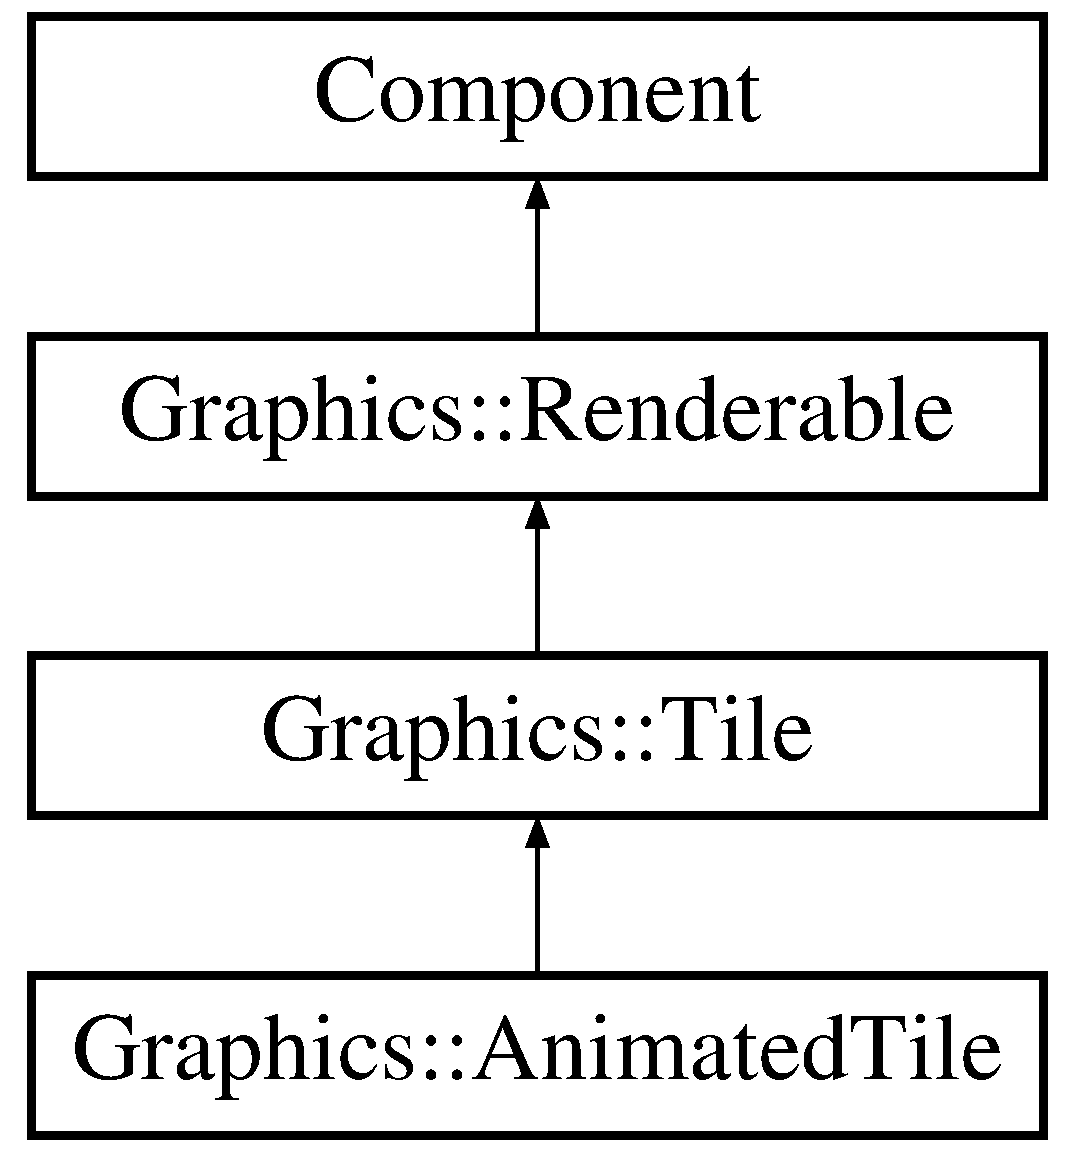
\includegraphics[height=4.000000cm]{class_graphics_1_1_animated_tile}
\end{center}
\end{figure}
\subsection*{Public Member Functions}
\begin{DoxyCompactItemize}
\item 
\hyperlink{class_graphics_1_1_animated_tile_a2845baac8df3cd5ceda7226d8c1da83a}{Animated\+Tile} (const unsigned int \hyperlink{class_graphics_1_1_renderable_aabfa91ebff7b10decd54119d663044ef}{vertex\+\_\+array\+\_\+object}, const \hyperlink{class_graphics_1_1_vertex_data}{Vertex\+Data} \&data)
\item 
virtual \hyperlink{class_graphics_1_1_animated_tile_a914ca23734bc692a35db7b1217418ef9}{$\sim$\+Animated\+Tile} ()
\item 
void \hyperlink{class_graphics_1_1_animated_tile_a7d4f7572d383943f06c81c86f87e06a2}{add\+Frame\+Front} (const glm\+::ivec2 \&frame\+\_\+pos, const unsigned int frame\+\_\+time)
\item 
void \hyperlink{class_graphics_1_1_animated_tile_a3b10e46f8f35a03e2c338cc20f9b7bd0}{add\+Frame\+Back} (const glm\+::ivec2 \&frame\+\_\+pos, const unsigned int frame\+\_\+time)
\item 
void \hyperlink{class_graphics_1_1_animated_tile_a92ab2aabe27674c38e7e7a31fd9b331e}{pop\+Frame\+Front} ()
\item 
void \hyperlink{class_graphics_1_1_animated_tile_a820c1aca5a701a43e50bdfbfe7324619}{pop\+Frame\+Back} ()
\item 
virtual void \hyperlink{class_graphics_1_1_animated_tile_ad82e39321244cc2e06ee3df527473aba}{on\+Start} () override
\item 
virtual const bool \hyperlink{class_graphics_1_1_animated_tile_a2c6f7cd3866cad84b73ea5da8b92b76e}{on\+Update} (const double delta) override
\begin{DoxyCompactList}\small\item\em \mbox{[}brief description\mbox{]} \end{DoxyCompactList}\item 
virtual const bool \hyperlink{class_graphics_1_1_animated_tile_a0b414dfdb18e4647652f8bb9334f9eee}{on\+Render} () override
\item 
virtual void \hyperlink{class_graphics_1_1_animated_tile_a9781b9b256a666a123fd2c050adb5118}{on\+Destroy} () override
\end{DoxyCompactItemize}
\subsection*{Private Attributes}
\begin{DoxyCompactItemize}
\item 
std\+::list$<$ std\+::pair$<$ glm\+::ivec2, unsigned int $>$ $>$ \hyperlink{class_graphics_1_1_animated_tile_a4d02a9bdd7576d1228b9ddf3eadec65c}{tile\+\_\+to\+\_\+time}
\item 
glm\+::vec2 \hyperlink{class_graphics_1_1_animated_tile_a6ceae6448ee26d0cd1b489795c55eb22}{multiplier}
\item 
float \hyperlink{class_graphics_1_1_animated_tile_a77a84617edf89f6b1576d4745bdd5d13}{frame\+\_\+time\+\_\+accumulator}
\end{DoxyCompactItemize}
\subsection*{Additional Inherited Members}


\subsection{Constructor \& Destructor Documentation}
\hypertarget{class_graphics_1_1_animated_tile_a2845baac8df3cd5ceda7226d8c1da83a}{}\index{Graphics\+::\+Animated\+Tile@{Graphics\+::\+Animated\+Tile}!Animated\+Tile@{Animated\+Tile}}
\index{Animated\+Tile@{Animated\+Tile}!Graphics\+::\+Animated\+Tile@{Graphics\+::\+Animated\+Tile}}
\subsubsection[{Animated\+Tile}]{\setlength{\rightskip}{0pt plus 5cm}Graphics\+::\+Animated\+Tile\+::\+Animated\+Tile (
\begin{DoxyParamCaption}
\item[{const unsigned int}]{vertex\+\_\+array\+\_\+object, }
\item[{const {\bf Vertex\+Data} \&}]{data}
\end{DoxyParamCaption}
)}\label{class_graphics_1_1_animated_tile_a2845baac8df3cd5ceda7226d8c1da83a}
\hypertarget{class_graphics_1_1_animated_tile_a914ca23734bc692a35db7b1217418ef9}{}\index{Graphics\+::\+Animated\+Tile@{Graphics\+::\+Animated\+Tile}!````~Animated\+Tile@{$\sim$\+Animated\+Tile}}
\index{````~Animated\+Tile@{$\sim$\+Animated\+Tile}!Graphics\+::\+Animated\+Tile@{Graphics\+::\+Animated\+Tile}}
\subsubsection[{$\sim$\+Animated\+Tile}]{\setlength{\rightskip}{0pt plus 5cm}Graphics\+::\+Animated\+Tile\+::$\sim$\+Animated\+Tile (
\begin{DoxyParamCaption}
{}
\end{DoxyParamCaption}
)\hspace{0.3cm}{\ttfamily [virtual]}}\label{class_graphics_1_1_animated_tile_a914ca23734bc692a35db7b1217418ef9}


\subsection{Member Function Documentation}
\hypertarget{class_graphics_1_1_animated_tile_a3b10e46f8f35a03e2c338cc20f9b7bd0}{}\index{Graphics\+::\+Animated\+Tile@{Graphics\+::\+Animated\+Tile}!add\+Frame\+Back@{add\+Frame\+Back}}
\index{add\+Frame\+Back@{add\+Frame\+Back}!Graphics\+::\+Animated\+Tile@{Graphics\+::\+Animated\+Tile}}
\subsubsection[{add\+Frame\+Back}]{\setlength{\rightskip}{0pt plus 5cm}void Graphics\+::\+Animated\+Tile\+::add\+Frame\+Back (
\begin{DoxyParamCaption}
\item[{const glm\+::ivec2 \&}]{frame\+\_\+pos, }
\item[{const unsigned int}]{frame\+\_\+time}
\end{DoxyParamCaption}
)}\label{class_graphics_1_1_animated_tile_a3b10e46f8f35a03e2c338cc20f9b7bd0}
\hypertarget{class_graphics_1_1_animated_tile_a7d4f7572d383943f06c81c86f87e06a2}{}\index{Graphics\+::\+Animated\+Tile@{Graphics\+::\+Animated\+Tile}!add\+Frame\+Front@{add\+Frame\+Front}}
\index{add\+Frame\+Front@{add\+Frame\+Front}!Graphics\+::\+Animated\+Tile@{Graphics\+::\+Animated\+Tile}}
\subsubsection[{add\+Frame\+Front}]{\setlength{\rightskip}{0pt plus 5cm}void Graphics\+::\+Animated\+Tile\+::add\+Frame\+Front (
\begin{DoxyParamCaption}
\item[{const glm\+::ivec2 \&}]{frame\+\_\+pos, }
\item[{const unsigned int}]{frame\+\_\+time}
\end{DoxyParamCaption}
)}\label{class_graphics_1_1_animated_tile_a7d4f7572d383943f06c81c86f87e06a2}
\hypertarget{class_graphics_1_1_animated_tile_a9781b9b256a666a123fd2c050adb5118}{}\index{Graphics\+::\+Animated\+Tile@{Graphics\+::\+Animated\+Tile}!on\+Destroy@{on\+Destroy}}
\index{on\+Destroy@{on\+Destroy}!Graphics\+::\+Animated\+Tile@{Graphics\+::\+Animated\+Tile}}
\subsubsection[{on\+Destroy}]{\setlength{\rightskip}{0pt plus 5cm}void Graphics\+::\+Animated\+Tile\+::on\+Destroy (
\begin{DoxyParamCaption}
{}
\end{DoxyParamCaption}
)\hspace{0.3cm}{\ttfamily [override]}, {\ttfamily [virtual]}}\label{class_graphics_1_1_animated_tile_a9781b9b256a666a123fd2c050adb5118}


Reimplemented from \hyperlink{class_graphics_1_1_tile_a28f5bdfa2fc61b292dda7ec15316b981}{Graphics\+::\+Tile}.

\hypertarget{class_graphics_1_1_animated_tile_a0b414dfdb18e4647652f8bb9334f9eee}{}\index{Graphics\+::\+Animated\+Tile@{Graphics\+::\+Animated\+Tile}!on\+Render@{on\+Render}}
\index{on\+Render@{on\+Render}!Graphics\+::\+Animated\+Tile@{Graphics\+::\+Animated\+Tile}}
\subsubsection[{on\+Render}]{\setlength{\rightskip}{0pt plus 5cm}const bool Graphics\+::\+Animated\+Tile\+::on\+Render (
\begin{DoxyParamCaption}
{}
\end{DoxyParamCaption}
)\hspace{0.3cm}{\ttfamily [override]}, {\ttfamily [virtual]}}\label{class_graphics_1_1_animated_tile_a0b414dfdb18e4647652f8bb9334f9eee}


Reimplemented from \hyperlink{class_graphics_1_1_renderable_afafd0e6147c73090234670934bbb8cbb}{Graphics\+::\+Renderable}.

\hypertarget{class_graphics_1_1_animated_tile_ad82e39321244cc2e06ee3df527473aba}{}\index{Graphics\+::\+Animated\+Tile@{Graphics\+::\+Animated\+Tile}!on\+Start@{on\+Start}}
\index{on\+Start@{on\+Start}!Graphics\+::\+Animated\+Tile@{Graphics\+::\+Animated\+Tile}}
\subsubsection[{on\+Start}]{\setlength{\rightskip}{0pt plus 5cm}void Graphics\+::\+Animated\+Tile\+::on\+Start (
\begin{DoxyParamCaption}
{}
\end{DoxyParamCaption}
)\hspace{0.3cm}{\ttfamily [override]}, {\ttfamily [virtual]}}\label{class_graphics_1_1_animated_tile_ad82e39321244cc2e06ee3df527473aba}


Reimplemented from \hyperlink{class_graphics_1_1_renderable_a7433551970cd25e0241a4a5bb756ba50}{Graphics\+::\+Renderable}.

\hypertarget{class_graphics_1_1_animated_tile_a2c6f7cd3866cad84b73ea5da8b92b76e}{}\index{Graphics\+::\+Animated\+Tile@{Graphics\+::\+Animated\+Tile}!on\+Update@{on\+Update}}
\index{on\+Update@{on\+Update}!Graphics\+::\+Animated\+Tile@{Graphics\+::\+Animated\+Tile}}
\subsubsection[{on\+Update}]{\setlength{\rightskip}{0pt plus 5cm}const bool Graphics\+::\+Animated\+Tile\+::on\+Update (
\begin{DoxyParamCaption}
\item[{const double}]{delta}
\end{DoxyParamCaption}
)\hspace{0.3cm}{\ttfamily [override]}, {\ttfamily [virtual]}}\label{class_graphics_1_1_animated_tile_a2c6f7cd3866cad84b73ea5da8b92b76e}


\mbox{[}brief description\mbox{]} 

\mbox{[}long description\mbox{]} \begin{DoxyReturn}{Returns}
true if anything was updated, false if nothing was updated 
\end{DoxyReturn}


Reimplemented from \hyperlink{class_graphics_1_1_tile_a0311b1d9548f6badc9e81820b110cbb4}{Graphics\+::\+Tile}.

\hypertarget{class_graphics_1_1_animated_tile_a820c1aca5a701a43e50bdfbfe7324619}{}\index{Graphics\+::\+Animated\+Tile@{Graphics\+::\+Animated\+Tile}!pop\+Frame\+Back@{pop\+Frame\+Back}}
\index{pop\+Frame\+Back@{pop\+Frame\+Back}!Graphics\+::\+Animated\+Tile@{Graphics\+::\+Animated\+Tile}}
\subsubsection[{pop\+Frame\+Back}]{\setlength{\rightskip}{0pt plus 5cm}void Graphics\+::\+Animated\+Tile\+::pop\+Frame\+Back (
\begin{DoxyParamCaption}
{}
\end{DoxyParamCaption}
)}\label{class_graphics_1_1_animated_tile_a820c1aca5a701a43e50bdfbfe7324619}
\hypertarget{class_graphics_1_1_animated_tile_a92ab2aabe27674c38e7e7a31fd9b331e}{}\index{Graphics\+::\+Animated\+Tile@{Graphics\+::\+Animated\+Tile}!pop\+Frame\+Front@{pop\+Frame\+Front}}
\index{pop\+Frame\+Front@{pop\+Frame\+Front}!Graphics\+::\+Animated\+Tile@{Graphics\+::\+Animated\+Tile}}
\subsubsection[{pop\+Frame\+Front}]{\setlength{\rightskip}{0pt plus 5cm}void Graphics\+::\+Animated\+Tile\+::pop\+Frame\+Front (
\begin{DoxyParamCaption}
{}
\end{DoxyParamCaption}
)}\label{class_graphics_1_1_animated_tile_a92ab2aabe27674c38e7e7a31fd9b331e}


\subsection{Member Data Documentation}
\hypertarget{class_graphics_1_1_animated_tile_a77a84617edf89f6b1576d4745bdd5d13}{}\index{Graphics\+::\+Animated\+Tile@{Graphics\+::\+Animated\+Tile}!frame\+\_\+time\+\_\+accumulator@{frame\+\_\+time\+\_\+accumulator}}
\index{frame\+\_\+time\+\_\+accumulator@{frame\+\_\+time\+\_\+accumulator}!Graphics\+::\+Animated\+Tile@{Graphics\+::\+Animated\+Tile}}
\subsubsection[{frame\+\_\+time\+\_\+accumulator}]{\setlength{\rightskip}{0pt plus 5cm}float Graphics\+::\+Animated\+Tile\+::frame\+\_\+time\+\_\+accumulator\hspace{0.3cm}{\ttfamily [private]}}\label{class_graphics_1_1_animated_tile_a77a84617edf89f6b1576d4745bdd5d13}
\hypertarget{class_graphics_1_1_animated_tile_a6ceae6448ee26d0cd1b489795c55eb22}{}\index{Graphics\+::\+Animated\+Tile@{Graphics\+::\+Animated\+Tile}!multiplier@{multiplier}}
\index{multiplier@{multiplier}!Graphics\+::\+Animated\+Tile@{Graphics\+::\+Animated\+Tile}}
\subsubsection[{multiplier}]{\setlength{\rightskip}{0pt plus 5cm}glm\+::vec2 Graphics\+::\+Animated\+Tile\+::multiplier\hspace{0.3cm}{\ttfamily [private]}}\label{class_graphics_1_1_animated_tile_a6ceae6448ee26d0cd1b489795c55eb22}
\hypertarget{class_graphics_1_1_animated_tile_a4d02a9bdd7576d1228b9ddf3eadec65c}{}\index{Graphics\+::\+Animated\+Tile@{Graphics\+::\+Animated\+Tile}!tile\+\_\+to\+\_\+time@{tile\+\_\+to\+\_\+time}}
\index{tile\+\_\+to\+\_\+time@{tile\+\_\+to\+\_\+time}!Graphics\+::\+Animated\+Tile@{Graphics\+::\+Animated\+Tile}}
\subsubsection[{tile\+\_\+to\+\_\+time}]{\setlength{\rightskip}{0pt plus 5cm}std\+::list$<$std\+::pair$<$glm\+::ivec2, unsigned int$>$ $>$ Graphics\+::\+Animated\+Tile\+::tile\+\_\+to\+\_\+time\hspace{0.3cm}{\ttfamily [private]}}\label{class_graphics_1_1_animated_tile_a4d02a9bdd7576d1228b9ddf3eadec65c}


The documentation for this class was generated from the following files\+:\begin{DoxyCompactItemize}
\item 
src/graphics/\hyperlink{animated__tile_8h}{animated\+\_\+tile.\+h}\item 
src/graphics/\hyperlink{animated__tile_8cpp}{animated\+\_\+tile.\+cpp}\end{DoxyCompactItemize}

\hypertarget{struct_graphics_1_1_animation}{}\section{Graphics\+:\+:Animation Struct Reference}
\label{struct_graphics_1_1_animation}\index{Graphics\+::\+Animation@{Graphics\+::\+Animation}}


{\ttfamily \#include $<$renderable\+\_\+factory.\+h$>$}

\subsection*{Public Attributes}
\begin{DoxyCompactItemize}
\item 
std\+::shared\+\_\+ptr$<$ \hyperlink{class_graphics_1_1_animated_tile}{Animated\+Tile} $>$ \hyperlink{struct_graphics_1_1_animation_ac0f14390b964e2be6cc008d7f12e8f70}{tile}
\item 
std\+::string \hyperlink{struct_graphics_1_1_animation_af4ea267c0295aeaa58945bca4443c8ea}{sprite\+\_\+name}
\item 
std\+::string \hyperlink{struct_graphics_1_1_animation_a161abc31b182618b4c12f0eb3cf0034b}{animation\+\_\+name}
\end{DoxyCompactItemize}


\subsection{Member Data Documentation}
\hypertarget{struct_graphics_1_1_animation_a161abc31b182618b4c12f0eb3cf0034b}{}\index{Graphics\+::\+Animation@{Graphics\+::\+Animation}!animation\+\_\+name@{animation\+\_\+name}}
\index{animation\+\_\+name@{animation\+\_\+name}!Graphics\+::\+Animation@{Graphics\+::\+Animation}}
\subsubsection[{animation\+\_\+name}]{\setlength{\rightskip}{0pt plus 5cm}std\+::string Graphics\+::\+Animation\+::animation\+\_\+name}\label{struct_graphics_1_1_animation_a161abc31b182618b4c12f0eb3cf0034b}
\hypertarget{struct_graphics_1_1_animation_af4ea267c0295aeaa58945bca4443c8ea}{}\index{Graphics\+::\+Animation@{Graphics\+::\+Animation}!sprite\+\_\+name@{sprite\+\_\+name}}
\index{sprite\+\_\+name@{sprite\+\_\+name}!Graphics\+::\+Animation@{Graphics\+::\+Animation}}
\subsubsection[{sprite\+\_\+name}]{\setlength{\rightskip}{0pt plus 5cm}std\+::string Graphics\+::\+Animation\+::sprite\+\_\+name}\label{struct_graphics_1_1_animation_af4ea267c0295aeaa58945bca4443c8ea}
\hypertarget{struct_graphics_1_1_animation_ac0f14390b964e2be6cc008d7f12e8f70}{}\index{Graphics\+::\+Animation@{Graphics\+::\+Animation}!tile@{tile}}
\index{tile@{tile}!Graphics\+::\+Animation@{Graphics\+::\+Animation}}
\subsubsection[{tile}]{\setlength{\rightskip}{0pt plus 5cm}std\+::shared\+\_\+ptr$<${\bf Animated\+Tile}$>$ Graphics\+::\+Animation\+::tile}\label{struct_graphics_1_1_animation_ac0f14390b964e2be6cc008d7f12e8f70}


The documentation for this struct was generated from the following file\+:\begin{DoxyCompactItemize}
\item 
src/graphics/\hyperlink{renderable__factory_8h}{renderable\+\_\+factory.\+h}\end{DoxyCompactItemize}

\hypertarget{struct_graphics_1_1_animation_placeholder}{}\section{Graphics\+:\+:Animation\+Placeholder Struct Reference}
\label{struct_graphics_1_1_animation_placeholder}\index{Graphics\+::\+Animation\+Placeholder@{Graphics\+::\+Animation\+Placeholder}}


{\ttfamily \#include $<$renderable\+\_\+factory.\+h$>$}

\subsection*{Public Attributes}
\begin{DoxyCompactItemize}
\item 
std\+::string \hyperlink{struct_graphics_1_1_animation_placeholder_aa6d0960d3bf182a8ce0047c2c2a180ed}{sprite\+\_\+name}
\item 
std\+::string \hyperlink{struct_graphics_1_1_animation_placeholder_ad5eae21e0490c802c1cf3e890e9000a8}{default\+\_\+animation}
\item 
int \hyperlink{struct_graphics_1_1_animation_placeholder_aed910a3665ceb34c24ea8daaac2b8d6f}{x\+\_\+pos}
\item 
int \hyperlink{struct_graphics_1_1_animation_placeholder_ad65e0d16937e548f1a4cc09c1d6e973a}{y\+\_\+pos}
\item 
int \hyperlink{struct_graphics_1_1_animation_placeholder_acc9e536b7002c04adc264abf55d51225}{z\+\_\+order}
\end{DoxyCompactItemize}


\subsection{Member Data Documentation}
\hypertarget{struct_graphics_1_1_animation_placeholder_ad5eae21e0490c802c1cf3e890e9000a8}{}\index{Graphics\+::\+Animation\+Placeholder@{Graphics\+::\+Animation\+Placeholder}!default\+\_\+animation@{default\+\_\+animation}}
\index{default\+\_\+animation@{default\+\_\+animation}!Graphics\+::\+Animation\+Placeholder@{Graphics\+::\+Animation\+Placeholder}}
\subsubsection[{default\+\_\+animation}]{\setlength{\rightskip}{0pt plus 5cm}std\+::string Graphics\+::\+Animation\+Placeholder\+::default\+\_\+animation}\label{struct_graphics_1_1_animation_placeholder_ad5eae21e0490c802c1cf3e890e9000a8}
\hypertarget{struct_graphics_1_1_animation_placeholder_aa6d0960d3bf182a8ce0047c2c2a180ed}{}\index{Graphics\+::\+Animation\+Placeholder@{Graphics\+::\+Animation\+Placeholder}!sprite\+\_\+name@{sprite\+\_\+name}}
\index{sprite\+\_\+name@{sprite\+\_\+name}!Graphics\+::\+Animation\+Placeholder@{Graphics\+::\+Animation\+Placeholder}}
\subsubsection[{sprite\+\_\+name}]{\setlength{\rightskip}{0pt plus 5cm}std\+::string Graphics\+::\+Animation\+Placeholder\+::sprite\+\_\+name}\label{struct_graphics_1_1_animation_placeholder_aa6d0960d3bf182a8ce0047c2c2a180ed}
\hypertarget{struct_graphics_1_1_animation_placeholder_aed910a3665ceb34c24ea8daaac2b8d6f}{}\index{Graphics\+::\+Animation\+Placeholder@{Graphics\+::\+Animation\+Placeholder}!x\+\_\+pos@{x\+\_\+pos}}
\index{x\+\_\+pos@{x\+\_\+pos}!Graphics\+::\+Animation\+Placeholder@{Graphics\+::\+Animation\+Placeholder}}
\subsubsection[{x\+\_\+pos}]{\setlength{\rightskip}{0pt plus 5cm}int Graphics\+::\+Animation\+Placeholder\+::x\+\_\+pos}\label{struct_graphics_1_1_animation_placeholder_aed910a3665ceb34c24ea8daaac2b8d6f}
\hypertarget{struct_graphics_1_1_animation_placeholder_ad65e0d16937e548f1a4cc09c1d6e973a}{}\index{Graphics\+::\+Animation\+Placeholder@{Graphics\+::\+Animation\+Placeholder}!y\+\_\+pos@{y\+\_\+pos}}
\index{y\+\_\+pos@{y\+\_\+pos}!Graphics\+::\+Animation\+Placeholder@{Graphics\+::\+Animation\+Placeholder}}
\subsubsection[{y\+\_\+pos}]{\setlength{\rightskip}{0pt plus 5cm}int Graphics\+::\+Animation\+Placeholder\+::y\+\_\+pos}\label{struct_graphics_1_1_animation_placeholder_ad65e0d16937e548f1a4cc09c1d6e973a}
\hypertarget{struct_graphics_1_1_animation_placeholder_acc9e536b7002c04adc264abf55d51225}{}\index{Graphics\+::\+Animation\+Placeholder@{Graphics\+::\+Animation\+Placeholder}!z\+\_\+order@{z\+\_\+order}}
\index{z\+\_\+order@{z\+\_\+order}!Graphics\+::\+Animation\+Placeholder@{Graphics\+::\+Animation\+Placeholder}}
\subsubsection[{z\+\_\+order}]{\setlength{\rightskip}{0pt plus 5cm}int Graphics\+::\+Animation\+Placeholder\+::z\+\_\+order}\label{struct_graphics_1_1_animation_placeholder_acc9e536b7002c04adc264abf55d51225}


The documentation for this struct was generated from the following file\+:\begin{DoxyCompactItemize}
\item 
src/graphics/\hyperlink{renderable__factory_8h}{renderable\+\_\+factory.\+h}\end{DoxyCompactItemize}

\hypertarget{class_graphics_1_1_base_attribute_trait}{}\section{Graphics\+:\+:Base\+Attribute\+Trait Class Reference}
\label{class_graphics_1_1_base_attribute_trait}\index{Graphics\+::\+Base\+Attribute\+Trait@{Graphics\+::\+Base\+Attribute\+Trait}}


{\ttfamily \#include $<$base\+\_\+attribute\+\_\+trait.\+h$>$}

Inheritance diagram for Graphics\+:\+:Base\+Attribute\+Trait\+:\begin{figure}[H]
\begin{center}
\leavevmode
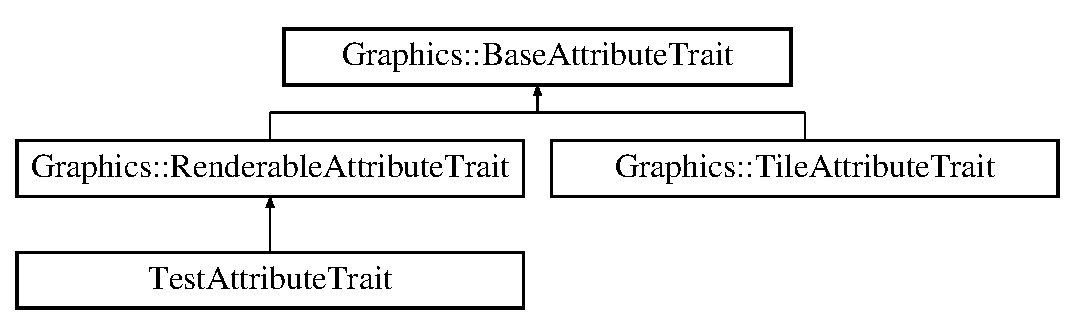
\includegraphics[height=3.000000cm]{class_graphics_1_1_base_attribute_trait}
\end{center}
\end{figure}
\subsection*{Public Member Functions}
\begin{DoxyCompactItemize}
\item 
virtual const std\+::map$<$ \hyperlink{class_graphics_1_1_vertex_data_a50e88236939dc2a3ec4df7aeb728620e}{Vertex\+Data\+::\+D\+A\+T\+A\+\_\+\+T\+Y\+P\+E}, unsigned int $>$ \hyperlink{class_graphics_1_1_base_attribute_trait_a7f43cabd619b64be1a0056e0fe568cf5}{operator()} () const noexcept=0
\end{DoxyCompactItemize}


\subsection{Member Function Documentation}
\hypertarget{class_graphics_1_1_base_attribute_trait_a7f43cabd619b64be1a0056e0fe568cf5}{}\index{Graphics\+::\+Base\+Attribute\+Trait@{Graphics\+::\+Base\+Attribute\+Trait}!operator()@{operator()}}
\index{operator()@{operator()}!Graphics\+::\+Base\+Attribute\+Trait@{Graphics\+::\+Base\+Attribute\+Trait}}
\subsubsection[{operator()}]{\setlength{\rightskip}{0pt plus 5cm}virtual const std\+::map$<${\bf Vertex\+Data\+::\+D\+A\+T\+A\+\_\+\+T\+Y\+P\+E}, unsigned int$>$ Graphics\+::\+Base\+Attribute\+Trait\+::operator() (
\begin{DoxyParamCaption}
{}
\end{DoxyParamCaption}
) const\hspace{0.3cm}{\ttfamily [pure virtual]}, {\ttfamily [noexcept]}}\label{class_graphics_1_1_base_attribute_trait_a7f43cabd619b64be1a0056e0fe568cf5}


Implemented in \hyperlink{class_test_attribute_trait_af121ef5fbd5bcda4bbbc7fdadd5599c8}{Test\+Attribute\+Trait}, \hyperlink{class_graphics_1_1_tile_attribute_trait_a5c217a080f9b52799ad6c9e2ffaa06f5}{Graphics\+::\+Tile\+Attribute\+Trait}, and \hyperlink{class_graphics_1_1_renderable_attribute_trait_a44401f624ace1dc71220e7064db92465}{Graphics\+::\+Renderable\+Attribute\+Trait}.



The documentation for this class was generated from the following file\+:\begin{DoxyCompactItemize}
\item 
src/graphics/\hyperlink{base__attribute__trait_8h}{base\+\_\+attribute\+\_\+trait.\+h}\end{DoxyCompactItemize}

\hypertarget{class_graphics_1_1_base_sampler}{}\section{Graphics\+:\+:Base\+Sampler Class Reference}
\label{class_graphics_1_1_base_sampler}\index{Graphics\+::\+Base\+Sampler@{Graphics\+::\+Base\+Sampler}}


{\ttfamily \#include $<$base\+\_\+sampler.\+h$>$}

\subsection*{Public Member Functions}
\begin{DoxyCompactItemize}
\item 
\hyperlink{class_graphics_1_1_base_sampler_afc353f064c976666a324a1052073505a}{Base\+Sampler} ()
\item 
virtual \hyperlink{class_graphics_1_1_base_sampler_adab45fb9ec695ae6e4ee42457995be9a}{$\sim$\+Base\+Sampler} ()
\item 
virtual void \hyperlink{class_graphics_1_1_base_sampler_afdcf5117f5f566924c6a8a2e0286f713}{bind} (const unsigned int texture\+\_\+unit)
\item 
virtual const unsigned int \hyperlink{class_graphics_1_1_base_sampler_a77ad273116e26d1404fb7914d4047416}{get\+Sampler\+Object} () const noexcept
\end{DoxyCompactItemize}
\subsection*{Private Attributes}
\begin{DoxyCompactItemize}
\item 
unsigned int \hyperlink{class_graphics_1_1_base_sampler_a0c1d724ce8b7d59aafdd27cd57d2c45c}{sampler\+\_\+object}
\end{DoxyCompactItemize}


\subsection{Constructor \& Destructor Documentation}
\hypertarget{class_graphics_1_1_base_sampler_afc353f064c976666a324a1052073505a}{}\index{Graphics\+::\+Base\+Sampler@{Graphics\+::\+Base\+Sampler}!Base\+Sampler@{Base\+Sampler}}
\index{Base\+Sampler@{Base\+Sampler}!Graphics\+::\+Base\+Sampler@{Graphics\+::\+Base\+Sampler}}
\subsubsection[{Base\+Sampler}]{\setlength{\rightskip}{0pt plus 5cm}Graphics\+::\+Base\+Sampler\+::\+Base\+Sampler (
\begin{DoxyParamCaption}
{}
\end{DoxyParamCaption}
)}\label{class_graphics_1_1_base_sampler_afc353f064c976666a324a1052073505a}
\hypertarget{class_graphics_1_1_base_sampler_adab45fb9ec695ae6e4ee42457995be9a}{}\index{Graphics\+::\+Base\+Sampler@{Graphics\+::\+Base\+Sampler}!````~Base\+Sampler@{$\sim$\+Base\+Sampler}}
\index{````~Base\+Sampler@{$\sim$\+Base\+Sampler}!Graphics\+::\+Base\+Sampler@{Graphics\+::\+Base\+Sampler}}
\subsubsection[{$\sim$\+Base\+Sampler}]{\setlength{\rightskip}{0pt plus 5cm}Graphics\+::\+Base\+Sampler\+::$\sim$\+Base\+Sampler (
\begin{DoxyParamCaption}
{}
\end{DoxyParamCaption}
)\hspace{0.3cm}{\ttfamily [virtual]}}\label{class_graphics_1_1_base_sampler_adab45fb9ec695ae6e4ee42457995be9a}


\subsection{Member Function Documentation}
\hypertarget{class_graphics_1_1_base_sampler_afdcf5117f5f566924c6a8a2e0286f713}{}\index{Graphics\+::\+Base\+Sampler@{Graphics\+::\+Base\+Sampler}!bind@{bind}}
\index{bind@{bind}!Graphics\+::\+Base\+Sampler@{Graphics\+::\+Base\+Sampler}}
\subsubsection[{bind}]{\setlength{\rightskip}{0pt plus 5cm}void Graphics\+::\+Base\+Sampler\+::bind (
\begin{DoxyParamCaption}
\item[{const unsigned int}]{texture\+\_\+unit}
\end{DoxyParamCaption}
)\hspace{0.3cm}{\ttfamily [virtual]}}\label{class_graphics_1_1_base_sampler_afdcf5117f5f566924c6a8a2e0286f713}
\hypertarget{class_graphics_1_1_base_sampler_a77ad273116e26d1404fb7914d4047416}{}\index{Graphics\+::\+Base\+Sampler@{Graphics\+::\+Base\+Sampler}!get\+Sampler\+Object@{get\+Sampler\+Object}}
\index{get\+Sampler\+Object@{get\+Sampler\+Object}!Graphics\+::\+Base\+Sampler@{Graphics\+::\+Base\+Sampler}}
\subsubsection[{get\+Sampler\+Object}]{\setlength{\rightskip}{0pt plus 5cm}const unsigned int Graphics\+::\+Base\+Sampler\+::get\+Sampler\+Object (
\begin{DoxyParamCaption}
{}
\end{DoxyParamCaption}
) const\hspace{0.3cm}{\ttfamily [virtual]}, {\ttfamily [noexcept]}}\label{class_graphics_1_1_base_sampler_a77ad273116e26d1404fb7914d4047416}


\subsection{Member Data Documentation}
\hypertarget{class_graphics_1_1_base_sampler_a0c1d724ce8b7d59aafdd27cd57d2c45c}{}\index{Graphics\+::\+Base\+Sampler@{Graphics\+::\+Base\+Sampler}!sampler\+\_\+object@{sampler\+\_\+object}}
\index{sampler\+\_\+object@{sampler\+\_\+object}!Graphics\+::\+Base\+Sampler@{Graphics\+::\+Base\+Sampler}}
\subsubsection[{sampler\+\_\+object}]{\setlength{\rightskip}{0pt plus 5cm}unsigned int Graphics\+::\+Base\+Sampler\+::sampler\+\_\+object\hspace{0.3cm}{\ttfamily [private]}}\label{class_graphics_1_1_base_sampler_a0c1d724ce8b7d59aafdd27cd57d2c45c}


The documentation for this class was generated from the following files\+:\begin{DoxyCompactItemize}
\item 
src/graphics/\hyperlink{base__sampler_8h}{base\+\_\+sampler.\+h}\item 
src/graphics/\hyperlink{base__sampler_8cpp}{base\+\_\+sampler.\+cpp}\end{DoxyCompactItemize}

\hypertarget{class_graphics_1_1_base_texture}{}\section{Graphics\+:\+:Base\+Texture Class Reference}
\label{class_graphics_1_1_base_texture}\index{Graphics\+::\+Base\+Texture@{Graphics\+::\+Base\+Texture}}


{\ttfamily \#include $<$base\+\_\+texture.\+h$>$}

\subsection*{Public Member Functions}
\begin{DoxyCompactItemize}
\item 
\hyperlink{class_graphics_1_1_base_texture_ae44fed159354650aee7f3e6f5d0b6477}{Base\+Texture} ()=delete
\item 
\hyperlink{class_graphics_1_1_base_texture_a7c9782999136f0101fcf5d0f6b13f006}{Base\+Texture} (const std\+::string \&\hyperlink{class_graphics_1_1_base_texture_a00bca25b10d3fe76e3f415606d302074}{texture\+\_\+uniform\+\_\+name}, const G\+Lenum \hyperlink{class_graphics_1_1_base_texture_a8541c8b38644380478955b823792b4d6}{texture\+\_\+type}, const unsigned int unit)
\item 
\hyperlink{class_graphics_1_1_base_texture_ac155c802b27ab8bbfc7dc9d2bb80dbd1}{$\sim$\+Base\+Texture} ()
\item 
const unsigned int \hyperlink{class_graphics_1_1_base_texture_aefa56cd236ec814799cc2b8c7d5a3508}{get\+Width} () const noexcept
\item 
const unsigned int \hyperlink{class_graphics_1_1_base_texture_a97d805fa4028b5864ca7a74fdb2fa915}{get\+Height} () const noexcept
\item 
const std\+::string \hyperlink{class_graphics_1_1_base_texture_ae01476d4da0efbdeffb264c5a0096d7d}{get\+Texture\+Uniform\+Name} () const noexcept
\item 
virtual const bool \hyperlink{class_graphics_1_1_base_texture_a32681ccc99ff4a4704172f9d365ea282}{load} (const std\+::string \&filename)
\item 
virtual void \hyperlink{class_graphics_1_1_base_texture_a564efe01e99f97729602ad1974d1ed38}{set\+Sampler} (const std\+::shared\+\_\+ptr$<$ \hyperlink{class_graphics_1_1_base_sampler}{Base\+Sampler} $>$ \hyperlink{class_graphics_1_1_base_texture_a7232ffaf919587d39516dcbd3f2659bd}{sampler})
\item 
virtual void \hyperlink{class_graphics_1_1_base_texture_a10e4a4b5eda51f85018bd64322e55532}{bind} ()
\item 
virtual const unsigned int \hyperlink{class_graphics_1_1_base_texture_a41bde844f513682641852da44f2f36a0}{get\+Texture\+Object} () const noexcept
\item 
virtual const unsigned int \hyperlink{class_graphics_1_1_base_texture_aaed0ad8a0ec7cc99943786aeebc2f3aa}{get\+Texture\+Unit} () const noexcept
\item 
virtual const std\+::shared\+\_\+ptr$<$ \hyperlink{class_graphics_1_1_base_sampler}{Base\+Sampler} $>$ \hyperlink{class_graphics_1_1_base_texture_a2ec731186e9afd266bc052aead7b15e8}{get\+Sampler} () const noexcept
\item 
virtual const bool \hyperlink{class_graphics_1_1_base_texture_a41e628cfd60b58269b088bc8538515bb}{is\+Loaded} () const noexcept
\end{DoxyCompactItemize}
\subsection*{Private Attributes}
\begin{DoxyCompactItemize}
\item 
unsigned int \hyperlink{class_graphics_1_1_base_texture_a30d08898d1d01c9960061dc2c8a98091}{texture\+\_\+unit}
\item 
unsigned int \hyperlink{class_graphics_1_1_base_texture_a2303afbe9f67a54922741d2c946b105f}{texture\+\_\+object}
\item 
G\+Lenum \hyperlink{class_graphics_1_1_base_texture_a8541c8b38644380478955b823792b4d6}{texture\+\_\+type}
\item 
std\+::shared\+\_\+ptr$<$ \hyperlink{class_graphics_1_1_base_sampler}{Base\+Sampler} $>$ \hyperlink{class_graphics_1_1_base_texture_a7232ffaf919587d39516dcbd3f2659bd}{sampler}
\item 
bool \hyperlink{class_graphics_1_1_base_texture_a1765fd6190e0a14c93f173e8693d07b2}{loaded}
\item 
unsigned int \hyperlink{class_graphics_1_1_base_texture_ad2790b49e5eab93516a8097c8f9dd422}{width}
\item 
unsigned int \hyperlink{class_graphics_1_1_base_texture_a8790d792749a6d25d18753880451baf8}{height}
\item 
std\+::string \hyperlink{class_graphics_1_1_base_texture_a00bca25b10d3fe76e3f415606d302074}{texture\+\_\+uniform\+\_\+name}
\end{DoxyCompactItemize}


\subsection{Constructor \& Destructor Documentation}
\hypertarget{class_graphics_1_1_base_texture_ae44fed159354650aee7f3e6f5d0b6477}{}\index{Graphics\+::\+Base\+Texture@{Graphics\+::\+Base\+Texture}!Base\+Texture@{Base\+Texture}}
\index{Base\+Texture@{Base\+Texture}!Graphics\+::\+Base\+Texture@{Graphics\+::\+Base\+Texture}}
\subsubsection[{Base\+Texture}]{\setlength{\rightskip}{0pt plus 5cm}Graphics\+::\+Base\+Texture\+::\+Base\+Texture (
\begin{DoxyParamCaption}
{}
\end{DoxyParamCaption}
)\hspace{0.3cm}{\ttfamily [delete]}}\label{class_graphics_1_1_base_texture_ae44fed159354650aee7f3e6f5d0b6477}
\hypertarget{class_graphics_1_1_base_texture_a7c9782999136f0101fcf5d0f6b13f006}{}\index{Graphics\+::\+Base\+Texture@{Graphics\+::\+Base\+Texture}!Base\+Texture@{Base\+Texture}}
\index{Base\+Texture@{Base\+Texture}!Graphics\+::\+Base\+Texture@{Graphics\+::\+Base\+Texture}}
\subsubsection[{Base\+Texture}]{\setlength{\rightskip}{0pt plus 5cm}Graphics\+::\+Base\+Texture\+::\+Base\+Texture (
\begin{DoxyParamCaption}
\item[{const std\+::string \&}]{texture\+\_\+uniform\+\_\+name, }
\item[{const G\+Lenum}]{texture\+\_\+type, }
\item[{const unsigned int}]{unit}
\end{DoxyParamCaption}
)}\label{class_graphics_1_1_base_texture_a7c9782999136f0101fcf5d0f6b13f006}
\hypertarget{class_graphics_1_1_base_texture_ac155c802b27ab8bbfc7dc9d2bb80dbd1}{}\index{Graphics\+::\+Base\+Texture@{Graphics\+::\+Base\+Texture}!````~Base\+Texture@{$\sim$\+Base\+Texture}}
\index{````~Base\+Texture@{$\sim$\+Base\+Texture}!Graphics\+::\+Base\+Texture@{Graphics\+::\+Base\+Texture}}
\subsubsection[{$\sim$\+Base\+Texture}]{\setlength{\rightskip}{0pt plus 5cm}Graphics\+::\+Base\+Texture\+::$\sim$\+Base\+Texture (
\begin{DoxyParamCaption}
{}
\end{DoxyParamCaption}
)}\label{class_graphics_1_1_base_texture_ac155c802b27ab8bbfc7dc9d2bb80dbd1}


\subsection{Member Function Documentation}
\hypertarget{class_graphics_1_1_base_texture_a10e4a4b5eda51f85018bd64322e55532}{}\index{Graphics\+::\+Base\+Texture@{Graphics\+::\+Base\+Texture}!bind@{bind}}
\index{bind@{bind}!Graphics\+::\+Base\+Texture@{Graphics\+::\+Base\+Texture}}
\subsubsection[{bind}]{\setlength{\rightskip}{0pt plus 5cm}void Graphics\+::\+Base\+Texture\+::bind (
\begin{DoxyParamCaption}
{}
\end{DoxyParamCaption}
)\hspace{0.3cm}{\ttfamily [virtual]}}\label{class_graphics_1_1_base_texture_a10e4a4b5eda51f85018bd64322e55532}
\hypertarget{class_graphics_1_1_base_texture_a97d805fa4028b5864ca7a74fdb2fa915}{}\index{Graphics\+::\+Base\+Texture@{Graphics\+::\+Base\+Texture}!get\+Height@{get\+Height}}
\index{get\+Height@{get\+Height}!Graphics\+::\+Base\+Texture@{Graphics\+::\+Base\+Texture}}
\subsubsection[{get\+Height}]{\setlength{\rightskip}{0pt plus 5cm}const unsigned int Graphics\+::\+Base\+Texture\+::get\+Height (
\begin{DoxyParamCaption}
{}
\end{DoxyParamCaption}
) const\hspace{0.3cm}{\ttfamily [noexcept]}}\label{class_graphics_1_1_base_texture_a97d805fa4028b5864ca7a74fdb2fa915}
\hypertarget{class_graphics_1_1_base_texture_a2ec731186e9afd266bc052aead7b15e8}{}\index{Graphics\+::\+Base\+Texture@{Graphics\+::\+Base\+Texture}!get\+Sampler@{get\+Sampler}}
\index{get\+Sampler@{get\+Sampler}!Graphics\+::\+Base\+Texture@{Graphics\+::\+Base\+Texture}}
\subsubsection[{get\+Sampler}]{\setlength{\rightskip}{0pt plus 5cm}const std\+::shared\+\_\+ptr$<$ {\bf Base\+Sampler} $>$ Graphics\+::\+Base\+Texture\+::get\+Sampler (
\begin{DoxyParamCaption}
{}
\end{DoxyParamCaption}
) const\hspace{0.3cm}{\ttfamily [virtual]}, {\ttfamily [noexcept]}}\label{class_graphics_1_1_base_texture_a2ec731186e9afd266bc052aead7b15e8}
\hypertarget{class_graphics_1_1_base_texture_a41bde844f513682641852da44f2f36a0}{}\index{Graphics\+::\+Base\+Texture@{Graphics\+::\+Base\+Texture}!get\+Texture\+Object@{get\+Texture\+Object}}
\index{get\+Texture\+Object@{get\+Texture\+Object}!Graphics\+::\+Base\+Texture@{Graphics\+::\+Base\+Texture}}
\subsubsection[{get\+Texture\+Object}]{\setlength{\rightskip}{0pt plus 5cm}const unsigned int Graphics\+::\+Base\+Texture\+::get\+Texture\+Object (
\begin{DoxyParamCaption}
{}
\end{DoxyParamCaption}
) const\hspace{0.3cm}{\ttfamily [virtual]}, {\ttfamily [noexcept]}}\label{class_graphics_1_1_base_texture_a41bde844f513682641852da44f2f36a0}
\hypertarget{class_graphics_1_1_base_texture_ae01476d4da0efbdeffb264c5a0096d7d}{}\index{Graphics\+::\+Base\+Texture@{Graphics\+::\+Base\+Texture}!get\+Texture\+Uniform\+Name@{get\+Texture\+Uniform\+Name}}
\index{get\+Texture\+Uniform\+Name@{get\+Texture\+Uniform\+Name}!Graphics\+::\+Base\+Texture@{Graphics\+::\+Base\+Texture}}
\subsubsection[{get\+Texture\+Uniform\+Name}]{\setlength{\rightskip}{0pt plus 5cm}const std\+::string Graphics\+::\+Base\+Texture\+::get\+Texture\+Uniform\+Name (
\begin{DoxyParamCaption}
{}
\end{DoxyParamCaption}
) const\hspace{0.3cm}{\ttfamily [noexcept]}}\label{class_graphics_1_1_base_texture_ae01476d4da0efbdeffb264c5a0096d7d}
\hypertarget{class_graphics_1_1_base_texture_aaed0ad8a0ec7cc99943786aeebc2f3aa}{}\index{Graphics\+::\+Base\+Texture@{Graphics\+::\+Base\+Texture}!get\+Texture\+Unit@{get\+Texture\+Unit}}
\index{get\+Texture\+Unit@{get\+Texture\+Unit}!Graphics\+::\+Base\+Texture@{Graphics\+::\+Base\+Texture}}
\subsubsection[{get\+Texture\+Unit}]{\setlength{\rightskip}{0pt plus 5cm}const unsigned int Graphics\+::\+Base\+Texture\+::get\+Texture\+Unit (
\begin{DoxyParamCaption}
{}
\end{DoxyParamCaption}
) const\hspace{0.3cm}{\ttfamily [virtual]}, {\ttfamily [noexcept]}}\label{class_graphics_1_1_base_texture_aaed0ad8a0ec7cc99943786aeebc2f3aa}
\hypertarget{class_graphics_1_1_base_texture_aefa56cd236ec814799cc2b8c7d5a3508}{}\index{Graphics\+::\+Base\+Texture@{Graphics\+::\+Base\+Texture}!get\+Width@{get\+Width}}
\index{get\+Width@{get\+Width}!Graphics\+::\+Base\+Texture@{Graphics\+::\+Base\+Texture}}
\subsubsection[{get\+Width}]{\setlength{\rightskip}{0pt plus 5cm}const unsigned int Graphics\+::\+Base\+Texture\+::get\+Width (
\begin{DoxyParamCaption}
{}
\end{DoxyParamCaption}
) const\hspace{0.3cm}{\ttfamily [noexcept]}}\label{class_graphics_1_1_base_texture_aefa56cd236ec814799cc2b8c7d5a3508}
\hypertarget{class_graphics_1_1_base_texture_a41e628cfd60b58269b088bc8538515bb}{}\index{Graphics\+::\+Base\+Texture@{Graphics\+::\+Base\+Texture}!is\+Loaded@{is\+Loaded}}
\index{is\+Loaded@{is\+Loaded}!Graphics\+::\+Base\+Texture@{Graphics\+::\+Base\+Texture}}
\subsubsection[{is\+Loaded}]{\setlength{\rightskip}{0pt plus 5cm}const bool Graphics\+::\+Base\+Texture\+::is\+Loaded (
\begin{DoxyParamCaption}
{}
\end{DoxyParamCaption}
) const\hspace{0.3cm}{\ttfamily [virtual]}, {\ttfamily [noexcept]}}\label{class_graphics_1_1_base_texture_a41e628cfd60b58269b088bc8538515bb}
\hypertarget{class_graphics_1_1_base_texture_a32681ccc99ff4a4704172f9d365ea282}{}\index{Graphics\+::\+Base\+Texture@{Graphics\+::\+Base\+Texture}!load@{load}}
\index{load@{load}!Graphics\+::\+Base\+Texture@{Graphics\+::\+Base\+Texture}}
\subsubsection[{load}]{\setlength{\rightskip}{0pt plus 5cm}const bool Graphics\+::\+Base\+Texture\+::load (
\begin{DoxyParamCaption}
\item[{const std\+::string \&}]{filename}
\end{DoxyParamCaption}
)\hspace{0.3cm}{\ttfamily [virtual]}}\label{class_graphics_1_1_base_texture_a32681ccc99ff4a4704172f9d365ea282}
\hypertarget{class_graphics_1_1_base_texture_a564efe01e99f97729602ad1974d1ed38}{}\index{Graphics\+::\+Base\+Texture@{Graphics\+::\+Base\+Texture}!set\+Sampler@{set\+Sampler}}
\index{set\+Sampler@{set\+Sampler}!Graphics\+::\+Base\+Texture@{Graphics\+::\+Base\+Texture}}
\subsubsection[{set\+Sampler}]{\setlength{\rightskip}{0pt plus 5cm}void Graphics\+::\+Base\+Texture\+::set\+Sampler (
\begin{DoxyParamCaption}
\item[{const std\+::shared\+\_\+ptr$<$ {\bf Base\+Sampler} $>$}]{sampler}
\end{DoxyParamCaption}
)\hspace{0.3cm}{\ttfamily [virtual]}}\label{class_graphics_1_1_base_texture_a564efe01e99f97729602ad1974d1ed38}


\subsection{Member Data Documentation}
\hypertarget{class_graphics_1_1_base_texture_a8790d792749a6d25d18753880451baf8}{}\index{Graphics\+::\+Base\+Texture@{Graphics\+::\+Base\+Texture}!height@{height}}
\index{height@{height}!Graphics\+::\+Base\+Texture@{Graphics\+::\+Base\+Texture}}
\subsubsection[{height}]{\setlength{\rightskip}{0pt plus 5cm}unsigned int Graphics\+::\+Base\+Texture\+::height\hspace{0.3cm}{\ttfamily [private]}}\label{class_graphics_1_1_base_texture_a8790d792749a6d25d18753880451baf8}
\hypertarget{class_graphics_1_1_base_texture_a1765fd6190e0a14c93f173e8693d07b2}{}\index{Graphics\+::\+Base\+Texture@{Graphics\+::\+Base\+Texture}!loaded@{loaded}}
\index{loaded@{loaded}!Graphics\+::\+Base\+Texture@{Graphics\+::\+Base\+Texture}}
\subsubsection[{loaded}]{\setlength{\rightskip}{0pt plus 5cm}bool Graphics\+::\+Base\+Texture\+::loaded\hspace{0.3cm}{\ttfamily [private]}}\label{class_graphics_1_1_base_texture_a1765fd6190e0a14c93f173e8693d07b2}
\hypertarget{class_graphics_1_1_base_texture_a7232ffaf919587d39516dcbd3f2659bd}{}\index{Graphics\+::\+Base\+Texture@{Graphics\+::\+Base\+Texture}!sampler@{sampler}}
\index{sampler@{sampler}!Graphics\+::\+Base\+Texture@{Graphics\+::\+Base\+Texture}}
\subsubsection[{sampler}]{\setlength{\rightskip}{0pt plus 5cm}std\+::shared\+\_\+ptr$<${\bf Base\+Sampler}$>$ Graphics\+::\+Base\+Texture\+::sampler\hspace{0.3cm}{\ttfamily [private]}}\label{class_graphics_1_1_base_texture_a7232ffaf919587d39516dcbd3f2659bd}
\hypertarget{class_graphics_1_1_base_texture_a2303afbe9f67a54922741d2c946b105f}{}\index{Graphics\+::\+Base\+Texture@{Graphics\+::\+Base\+Texture}!texture\+\_\+object@{texture\+\_\+object}}
\index{texture\+\_\+object@{texture\+\_\+object}!Graphics\+::\+Base\+Texture@{Graphics\+::\+Base\+Texture}}
\subsubsection[{texture\+\_\+object}]{\setlength{\rightskip}{0pt plus 5cm}unsigned int Graphics\+::\+Base\+Texture\+::texture\+\_\+object\hspace{0.3cm}{\ttfamily [private]}}\label{class_graphics_1_1_base_texture_a2303afbe9f67a54922741d2c946b105f}
\hypertarget{class_graphics_1_1_base_texture_a8541c8b38644380478955b823792b4d6}{}\index{Graphics\+::\+Base\+Texture@{Graphics\+::\+Base\+Texture}!texture\+\_\+type@{texture\+\_\+type}}
\index{texture\+\_\+type@{texture\+\_\+type}!Graphics\+::\+Base\+Texture@{Graphics\+::\+Base\+Texture}}
\subsubsection[{texture\+\_\+type}]{\setlength{\rightskip}{0pt plus 5cm}G\+Lenum Graphics\+::\+Base\+Texture\+::texture\+\_\+type\hspace{0.3cm}{\ttfamily [private]}}\label{class_graphics_1_1_base_texture_a8541c8b38644380478955b823792b4d6}
\hypertarget{class_graphics_1_1_base_texture_a00bca25b10d3fe76e3f415606d302074}{}\index{Graphics\+::\+Base\+Texture@{Graphics\+::\+Base\+Texture}!texture\+\_\+uniform\+\_\+name@{texture\+\_\+uniform\+\_\+name}}
\index{texture\+\_\+uniform\+\_\+name@{texture\+\_\+uniform\+\_\+name}!Graphics\+::\+Base\+Texture@{Graphics\+::\+Base\+Texture}}
\subsubsection[{texture\+\_\+uniform\+\_\+name}]{\setlength{\rightskip}{0pt plus 5cm}std\+::string Graphics\+::\+Base\+Texture\+::texture\+\_\+uniform\+\_\+name\hspace{0.3cm}{\ttfamily [private]}}\label{class_graphics_1_1_base_texture_a00bca25b10d3fe76e3f415606d302074}
\hypertarget{class_graphics_1_1_base_texture_a30d08898d1d01c9960061dc2c8a98091}{}\index{Graphics\+::\+Base\+Texture@{Graphics\+::\+Base\+Texture}!texture\+\_\+unit@{texture\+\_\+unit}}
\index{texture\+\_\+unit@{texture\+\_\+unit}!Graphics\+::\+Base\+Texture@{Graphics\+::\+Base\+Texture}}
\subsubsection[{texture\+\_\+unit}]{\setlength{\rightskip}{0pt plus 5cm}unsigned int Graphics\+::\+Base\+Texture\+::texture\+\_\+unit\hspace{0.3cm}{\ttfamily [private]}}\label{class_graphics_1_1_base_texture_a30d08898d1d01c9960061dc2c8a98091}
\hypertarget{class_graphics_1_1_base_texture_ad2790b49e5eab93516a8097c8f9dd422}{}\index{Graphics\+::\+Base\+Texture@{Graphics\+::\+Base\+Texture}!width@{width}}
\index{width@{width}!Graphics\+::\+Base\+Texture@{Graphics\+::\+Base\+Texture}}
\subsubsection[{width}]{\setlength{\rightskip}{0pt plus 5cm}unsigned int Graphics\+::\+Base\+Texture\+::width\hspace{0.3cm}{\ttfamily [private]}}\label{class_graphics_1_1_base_texture_ad2790b49e5eab93516a8097c8f9dd422}


The documentation for this class was generated from the following files\+:\begin{DoxyCompactItemize}
\item 
src/graphics/\hyperlink{base__texture_8h}{base\+\_\+texture.\+h}\item 
src/graphics/\hyperlink{base__texture_8cpp}{base\+\_\+texture.\+cpp}\end{DoxyCompactItemize}

\hypertarget{class_graphics_1_1_camera}{}\section{Graphics\+:\+:Camera Class Reference}
\label{class_graphics_1_1_camera}\index{Graphics\+::\+Camera@{Graphics\+::\+Camera}}


{\ttfamily \#include $<$camera.\+h$>$}

Inheritance diagram for Graphics\+:\+:Camera\+:\begin{figure}[H]
\begin{center}
\leavevmode
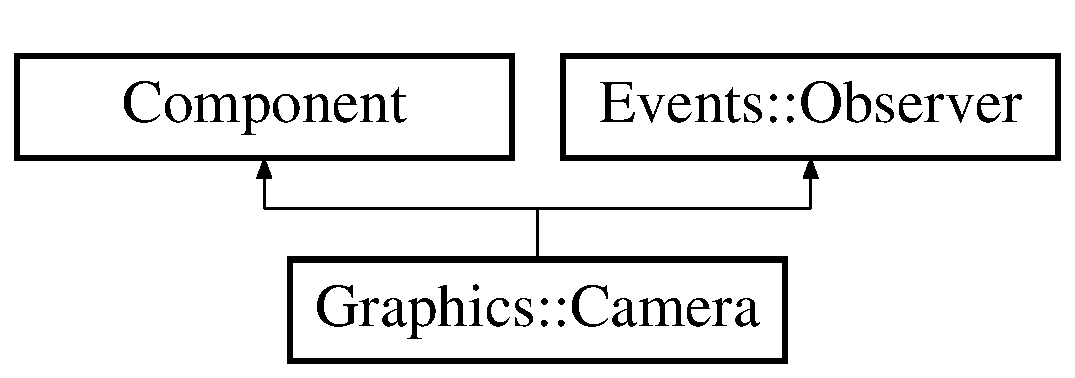
\includegraphics[height=2.000000cm]{class_graphics_1_1_camera}
\end{center}
\end{figure}
\subsection*{Public Member Functions}
\begin{DoxyCompactItemize}
\item 
\hyperlink{class_graphics_1_1_camera_a357a2294fe254fc1dd24061336f7fef9}{Camera} ()=delete
\item 
\hyperlink{class_graphics_1_1_camera_a4974bc917c6e7db4a9429e5ce3673b14}{Camera} (const std\+::shared\+\_\+ptr$<$ \hyperlink{class_graphics_1_1_shader_manager}{Shader\+Manager} $>$ \hyperlink{class_graphics_1_1_camera_a60d25d91283365ea01a54a81e0f9246b}{shader\+\_\+manager})
\item 
\hyperlink{class_graphics_1_1_camera_aef6471ed249e435e25bb80bbafad31cf}{Camera} (const std\+::shared\+\_\+ptr$<$ \hyperlink{class_graphics_1_1_shader_manager}{Shader\+Manager} $>$ \hyperlink{class_graphics_1_1_camera_a60d25d91283365ea01a54a81e0f9246b}{shader\+\_\+manager}, const float \hyperlink{class_graphics_1_1_camera_ae08e862d5cf284a8d28a5b5bebdf1d33}{viewport\+\_\+width}, const float \hyperlink{class_graphics_1_1_camera_acc8b30298da1779394bbafb91f5a7855}{viewport\+\_\+height}, const float \hyperlink{class_graphics_1_1_camera_ad4c61e1382447826985b5a5445379375}{near}=0.\+1, const float \hyperlink{class_graphics_1_1_camera_a1d6d4c2d74d4d25ef66900bf603e88af}{far}=1.\+0)
\item 
virtual void \hyperlink{class_graphics_1_1_camera_a37edadff497ff3966c2190b876bfe236}{on\+Start} () override
\item 
virtual const bool \hyperlink{class_graphics_1_1_camera_a0bfccb5623342c93f69b408937b87374}{on\+Update} (const double delta) override
\item 
virtual void \hyperlink{class_graphics_1_1_camera_a9d8ca67cbd7a586915fc6cfd303406de}{on\+Destroy} () override
\item 
void \hyperlink{class_graphics_1_1_camera_afd1785008e1ee71690749bf99a5d1e9a}{on\+Notify} (const \hyperlink{class_events_1_1_event}{Events\+::\+Event} \&event) override
\item 
void \hyperlink{class_graphics_1_1_camera_ad0ac1e840142be9747d4601132b99a89}{set\+Screen\+Padding\+In\+Tiles} (const int padding) noexcept
\item 
const int \hyperlink{class_graphics_1_1_camera_aaec05679e857e34c6066487c0bedcdd0}{get\+Screen\+Padding\+In\+Tiles} () const noexcept
\item 
void \hyperlink{class_graphics_1_1_camera_aaccd7b431b1fe0ff34cb5b012a51bfa1}{set\+Width} (const float width) noexcept
\item 
const float \hyperlink{class_graphics_1_1_camera_a3ad408f656300f71c96e426dd6a2229e}{get\+Width} () const noexcept
\item 
void \hyperlink{class_graphics_1_1_camera_ae99d2724d10610bda819b50d6caebc3b}{set\+Height} (const float height) noexcept
\item 
const float \hyperlink{class_graphics_1_1_camera_af74120d1b11dae8e05bfa36e14019a06}{get\+Height} () const noexcept
\item 
void \hyperlink{class_graphics_1_1_camera_a7c4ae1ab7d2193b474b0f21f7520048e}{set\+Near} (const float \hyperlink{class_graphics_1_1_camera_ad4c61e1382447826985b5a5445379375}{near}) noexcept
\item 
const float \hyperlink{class_graphics_1_1_camera_abb26f99ab2483da3ba991608fac0be78}{get\+Near} () const noexcept
\item 
void \hyperlink{class_graphics_1_1_camera_a28bcc186295608ede40f37950d2de4e3}{set\+Far} (const float \hyperlink{class_graphics_1_1_camera_a1d6d4c2d74d4d25ef66900bf603e88af}{far}) noexcept
\item 
const float \hyperlink{class_graphics_1_1_camera_a619c02f188c7eea0edefacdda440dff7}{get\+Far} () const noexcept
\item 
const bool \hyperlink{class_graphics_1_1_camera_a9a4015f5d7e54c8bf2ba248f72951578}{is\+Renderable\+Within} (std\+::shared\+\_\+ptr$<$ \hyperlink{class_graphics_1_1_renderable}{Renderable} $>$ renderable) const 
\end{DoxyCompactItemize}
\subsection*{Private Member Functions}
\begin{DoxyCompactItemize}
\item 
\hyperlink{class_transform}{Transform} \hyperlink{class_graphics_1_1_camera_a5a828597ad4c4534481db66c38900cf0}{negate\+Transform\+For\+Screen} (std\+::shared\+\_\+ptr$<$ \hyperlink{class_transform}{Transform} $>$ trans)
\end{DoxyCompactItemize}
\subsection*{Private Attributes}
\begin{DoxyCompactItemize}
\item 
glm\+::mat4 \hyperlink{class_graphics_1_1_camera_a7b168f8afa0098c51f64853605a08fc8}{projection\+\_\+matrix}
\item 
\hyperlink{class_transform}{Transform} \hyperlink{class_graphics_1_1_camera_af70f9f26e21cef48e41bb0b025b8528d}{last\+\_\+transform}
\item 
glm\+::mat4 \hyperlink{class_graphics_1_1_camera_a61b7cb1de65dc8a4f444598a71c3b853}{last\+\_\+projection\+\_\+matrix}
\item 
std\+::shared\+\_\+ptr$<$ \hyperlink{class_graphics_1_1_shader_manager}{Shader\+Manager} $>$ \hyperlink{class_graphics_1_1_camera_a60d25d91283365ea01a54a81e0f9246b}{shader\+\_\+manager}
\item 
float \hyperlink{class_graphics_1_1_camera_ae08e862d5cf284a8d28a5b5bebdf1d33}{viewport\+\_\+width}
\item 
float \hyperlink{class_graphics_1_1_camera_acc8b30298da1779394bbafb91f5a7855}{viewport\+\_\+height}
\item 
float \hyperlink{class_graphics_1_1_camera_ad4c61e1382447826985b5a5445379375}{near}
\item 
float \hyperlink{class_graphics_1_1_camera_a1d6d4c2d74d4d25ef66900bf603e88af}{far}
\item 
glm\+::vec2 \hyperlink{class_graphics_1_1_camera_aefe34c1354a1e2f45db923da5686e1d5}{velocity}
\item 
glm\+::vec2 \hyperlink{class_graphics_1_1_camera_a95457d183395bfd80e63ede6418f35f7}{target\+\_\+position}
\item 
int \hyperlink{class_graphics_1_1_camera_adce9d36698524aaeae74211059efc556}{screen\+\_\+padding\+\_\+in\+\_\+tiles}
\end{DoxyCompactItemize}
\subsection*{Additional Inherited Members}


\subsection{Constructor \& Destructor Documentation}
\hypertarget{class_graphics_1_1_camera_a357a2294fe254fc1dd24061336f7fef9}{}\index{Graphics\+::\+Camera@{Graphics\+::\+Camera}!Camera@{Camera}}
\index{Camera@{Camera}!Graphics\+::\+Camera@{Graphics\+::\+Camera}}
\subsubsection[{Camera}]{\setlength{\rightskip}{0pt plus 5cm}Graphics\+::\+Camera\+::\+Camera (
\begin{DoxyParamCaption}
{}
\end{DoxyParamCaption}
)\hspace{0.3cm}{\ttfamily [delete]}}\label{class_graphics_1_1_camera_a357a2294fe254fc1dd24061336f7fef9}
\hypertarget{class_graphics_1_1_camera_a4974bc917c6e7db4a9429e5ce3673b14}{}\index{Graphics\+::\+Camera@{Graphics\+::\+Camera}!Camera@{Camera}}
\index{Camera@{Camera}!Graphics\+::\+Camera@{Graphics\+::\+Camera}}
\subsubsection[{Camera}]{\setlength{\rightskip}{0pt plus 5cm}Graphics\+::\+Camera\+::\+Camera (
\begin{DoxyParamCaption}
\item[{const std\+::shared\+\_\+ptr$<$ {\bf Shader\+Manager} $>$}]{shader\+\_\+manager}
\end{DoxyParamCaption}
)}\label{class_graphics_1_1_camera_a4974bc917c6e7db4a9429e5ce3673b14}
\hypertarget{class_graphics_1_1_camera_aef6471ed249e435e25bb80bbafad31cf}{}\index{Graphics\+::\+Camera@{Graphics\+::\+Camera}!Camera@{Camera}}
\index{Camera@{Camera}!Graphics\+::\+Camera@{Graphics\+::\+Camera}}
\subsubsection[{Camera}]{\setlength{\rightskip}{0pt plus 5cm}Graphics\+::\+Camera\+::\+Camera (
\begin{DoxyParamCaption}
\item[{const std\+::shared\+\_\+ptr$<$ {\bf Shader\+Manager} $>$}]{shader\+\_\+manager, }
\item[{const float}]{viewport\+\_\+width, }
\item[{const float}]{viewport\+\_\+height, }
\item[{const float}]{near = {\ttfamily 0.1}, }
\item[{const float}]{far = {\ttfamily 1.0}}
\end{DoxyParamCaption}
)}\label{class_graphics_1_1_camera_aef6471ed249e435e25bb80bbafad31cf}


\subsection{Member Function Documentation}
\hypertarget{class_graphics_1_1_camera_a619c02f188c7eea0edefacdda440dff7}{}\index{Graphics\+::\+Camera@{Graphics\+::\+Camera}!get\+Far@{get\+Far}}
\index{get\+Far@{get\+Far}!Graphics\+::\+Camera@{Graphics\+::\+Camera}}
\subsubsection[{get\+Far}]{\setlength{\rightskip}{0pt plus 5cm}const float Graphics\+::\+Camera\+::get\+Far (
\begin{DoxyParamCaption}
{}
\end{DoxyParamCaption}
) const\hspace{0.3cm}{\ttfamily [noexcept]}}\label{class_graphics_1_1_camera_a619c02f188c7eea0edefacdda440dff7}
\hypertarget{class_graphics_1_1_camera_af74120d1b11dae8e05bfa36e14019a06}{}\index{Graphics\+::\+Camera@{Graphics\+::\+Camera}!get\+Height@{get\+Height}}
\index{get\+Height@{get\+Height}!Graphics\+::\+Camera@{Graphics\+::\+Camera}}
\subsubsection[{get\+Height}]{\setlength{\rightskip}{0pt plus 5cm}const float Graphics\+::\+Camera\+::get\+Height (
\begin{DoxyParamCaption}
{}
\end{DoxyParamCaption}
) const\hspace{0.3cm}{\ttfamily [noexcept]}}\label{class_graphics_1_1_camera_af74120d1b11dae8e05bfa36e14019a06}
\hypertarget{class_graphics_1_1_camera_abb26f99ab2483da3ba991608fac0be78}{}\index{Graphics\+::\+Camera@{Graphics\+::\+Camera}!get\+Near@{get\+Near}}
\index{get\+Near@{get\+Near}!Graphics\+::\+Camera@{Graphics\+::\+Camera}}
\subsubsection[{get\+Near}]{\setlength{\rightskip}{0pt plus 5cm}const float Graphics\+::\+Camera\+::get\+Near (
\begin{DoxyParamCaption}
{}
\end{DoxyParamCaption}
) const\hspace{0.3cm}{\ttfamily [noexcept]}}\label{class_graphics_1_1_camera_abb26f99ab2483da3ba991608fac0be78}
\hypertarget{class_graphics_1_1_camera_aaec05679e857e34c6066487c0bedcdd0}{}\index{Graphics\+::\+Camera@{Graphics\+::\+Camera}!get\+Screen\+Padding\+In\+Tiles@{get\+Screen\+Padding\+In\+Tiles}}
\index{get\+Screen\+Padding\+In\+Tiles@{get\+Screen\+Padding\+In\+Tiles}!Graphics\+::\+Camera@{Graphics\+::\+Camera}}
\subsubsection[{get\+Screen\+Padding\+In\+Tiles}]{\setlength{\rightskip}{0pt plus 5cm}const int Graphics\+::\+Camera\+::get\+Screen\+Padding\+In\+Tiles (
\begin{DoxyParamCaption}
{}
\end{DoxyParamCaption}
) const\hspace{0.3cm}{\ttfamily [noexcept]}}\label{class_graphics_1_1_camera_aaec05679e857e34c6066487c0bedcdd0}
\hypertarget{class_graphics_1_1_camera_a3ad408f656300f71c96e426dd6a2229e}{}\index{Graphics\+::\+Camera@{Graphics\+::\+Camera}!get\+Width@{get\+Width}}
\index{get\+Width@{get\+Width}!Graphics\+::\+Camera@{Graphics\+::\+Camera}}
\subsubsection[{get\+Width}]{\setlength{\rightskip}{0pt plus 5cm}const float Graphics\+::\+Camera\+::get\+Width (
\begin{DoxyParamCaption}
{}
\end{DoxyParamCaption}
) const\hspace{0.3cm}{\ttfamily [noexcept]}}\label{class_graphics_1_1_camera_a3ad408f656300f71c96e426dd6a2229e}
\hypertarget{class_graphics_1_1_camera_a9a4015f5d7e54c8bf2ba248f72951578}{}\index{Graphics\+::\+Camera@{Graphics\+::\+Camera}!is\+Renderable\+Within@{is\+Renderable\+Within}}
\index{is\+Renderable\+Within@{is\+Renderable\+Within}!Graphics\+::\+Camera@{Graphics\+::\+Camera}}
\subsubsection[{is\+Renderable\+Within}]{\setlength{\rightskip}{0pt plus 5cm}const bool Graphics\+::\+Camera\+::is\+Renderable\+Within (
\begin{DoxyParamCaption}
\item[{std\+::shared\+\_\+ptr$<$ {\bf Renderable} $>$}]{renderable}
\end{DoxyParamCaption}
) const}\label{class_graphics_1_1_camera_a9a4015f5d7e54c8bf2ba248f72951578}
\hypertarget{class_graphics_1_1_camera_a5a828597ad4c4534481db66c38900cf0}{}\index{Graphics\+::\+Camera@{Graphics\+::\+Camera}!negate\+Transform\+For\+Screen@{negate\+Transform\+For\+Screen}}
\index{negate\+Transform\+For\+Screen@{negate\+Transform\+For\+Screen}!Graphics\+::\+Camera@{Graphics\+::\+Camera}}
\subsubsection[{negate\+Transform\+For\+Screen}]{\setlength{\rightskip}{0pt plus 5cm}{\bf Transform} Graphics\+::\+Camera\+::negate\+Transform\+For\+Screen (
\begin{DoxyParamCaption}
\item[{std\+::shared\+\_\+ptr$<$ {\bf Transform} $>$}]{trans}
\end{DoxyParamCaption}
)\hspace{0.3cm}{\ttfamily [private]}}\label{class_graphics_1_1_camera_a5a828597ad4c4534481db66c38900cf0}
\hypertarget{class_graphics_1_1_camera_a9d8ca67cbd7a586915fc6cfd303406de}{}\index{Graphics\+::\+Camera@{Graphics\+::\+Camera}!on\+Destroy@{on\+Destroy}}
\index{on\+Destroy@{on\+Destroy}!Graphics\+::\+Camera@{Graphics\+::\+Camera}}
\subsubsection[{on\+Destroy}]{\setlength{\rightskip}{0pt plus 5cm}void Graphics\+::\+Camera\+::on\+Destroy (
\begin{DoxyParamCaption}
{}
\end{DoxyParamCaption}
)\hspace{0.3cm}{\ttfamily [override]}, {\ttfamily [virtual]}}\label{class_graphics_1_1_camera_a9d8ca67cbd7a586915fc6cfd303406de}


Implements \hyperlink{class_component_a2b198f27162a6caf63917e304295f892}{Component}.

\hypertarget{class_graphics_1_1_camera_afd1785008e1ee71690749bf99a5d1e9a}{}\index{Graphics\+::\+Camera@{Graphics\+::\+Camera}!on\+Notify@{on\+Notify}}
\index{on\+Notify@{on\+Notify}!Graphics\+::\+Camera@{Graphics\+::\+Camera}}
\subsubsection[{on\+Notify}]{\setlength{\rightskip}{0pt plus 5cm}void Graphics\+::\+Camera\+::on\+Notify (
\begin{DoxyParamCaption}
\item[{const {\bf Events\+::\+Event} \&}]{event}
\end{DoxyParamCaption}
)\hspace{0.3cm}{\ttfamily [override]}, {\ttfamily [virtual]}}\label{class_graphics_1_1_camera_afd1785008e1ee71690749bf99a5d1e9a}


Implements \hyperlink{class_events_1_1_observer_ad10e3ade9e803e9f706c5799da1d6525}{Events\+::\+Observer}.

\hypertarget{class_graphics_1_1_camera_a37edadff497ff3966c2190b876bfe236}{}\index{Graphics\+::\+Camera@{Graphics\+::\+Camera}!on\+Start@{on\+Start}}
\index{on\+Start@{on\+Start}!Graphics\+::\+Camera@{Graphics\+::\+Camera}}
\subsubsection[{on\+Start}]{\setlength{\rightskip}{0pt plus 5cm}void Graphics\+::\+Camera\+::on\+Start (
\begin{DoxyParamCaption}
{}
\end{DoxyParamCaption}
)\hspace{0.3cm}{\ttfamily [override]}, {\ttfamily [virtual]}}\label{class_graphics_1_1_camera_a37edadff497ff3966c2190b876bfe236}


Implements \hyperlink{class_component_a4a528a8790dbc141ffd0aba638b6dcc4}{Component}.

\hypertarget{class_graphics_1_1_camera_a0bfccb5623342c93f69b408937b87374}{}\index{Graphics\+::\+Camera@{Graphics\+::\+Camera}!on\+Update@{on\+Update}}
\index{on\+Update@{on\+Update}!Graphics\+::\+Camera@{Graphics\+::\+Camera}}
\subsubsection[{on\+Update}]{\setlength{\rightskip}{0pt plus 5cm}const bool Graphics\+::\+Camera\+::on\+Update (
\begin{DoxyParamCaption}
\item[{const double}]{delta}
\end{DoxyParamCaption}
)\hspace{0.3cm}{\ttfamily [override]}, {\ttfamily [virtual]}}\label{class_graphics_1_1_camera_a0bfccb5623342c93f69b408937b87374}


Implements \hyperlink{class_component_a8be284fccf4e97cee6705bd2d8f3705e}{Component}.

\hypertarget{class_graphics_1_1_camera_a28bcc186295608ede40f37950d2de4e3}{}\index{Graphics\+::\+Camera@{Graphics\+::\+Camera}!set\+Far@{set\+Far}}
\index{set\+Far@{set\+Far}!Graphics\+::\+Camera@{Graphics\+::\+Camera}}
\subsubsection[{set\+Far}]{\setlength{\rightskip}{0pt plus 5cm}void Graphics\+::\+Camera\+::set\+Far (
\begin{DoxyParamCaption}
\item[{const float}]{far}
\end{DoxyParamCaption}
)\hspace{0.3cm}{\ttfamily [noexcept]}}\label{class_graphics_1_1_camera_a28bcc186295608ede40f37950d2de4e3}
\hypertarget{class_graphics_1_1_camera_ae99d2724d10610bda819b50d6caebc3b}{}\index{Graphics\+::\+Camera@{Graphics\+::\+Camera}!set\+Height@{set\+Height}}
\index{set\+Height@{set\+Height}!Graphics\+::\+Camera@{Graphics\+::\+Camera}}
\subsubsection[{set\+Height}]{\setlength{\rightskip}{0pt plus 5cm}void Graphics\+::\+Camera\+::set\+Height (
\begin{DoxyParamCaption}
\item[{const float}]{height}
\end{DoxyParamCaption}
)\hspace{0.3cm}{\ttfamily [noexcept]}}\label{class_graphics_1_1_camera_ae99d2724d10610bda819b50d6caebc3b}
\hypertarget{class_graphics_1_1_camera_a7c4ae1ab7d2193b474b0f21f7520048e}{}\index{Graphics\+::\+Camera@{Graphics\+::\+Camera}!set\+Near@{set\+Near}}
\index{set\+Near@{set\+Near}!Graphics\+::\+Camera@{Graphics\+::\+Camera}}
\subsubsection[{set\+Near}]{\setlength{\rightskip}{0pt plus 5cm}void Graphics\+::\+Camera\+::set\+Near (
\begin{DoxyParamCaption}
\item[{const float}]{near}
\end{DoxyParamCaption}
)\hspace{0.3cm}{\ttfamily [noexcept]}}\label{class_graphics_1_1_camera_a7c4ae1ab7d2193b474b0f21f7520048e}
\hypertarget{class_graphics_1_1_camera_ad0ac1e840142be9747d4601132b99a89}{}\index{Graphics\+::\+Camera@{Graphics\+::\+Camera}!set\+Screen\+Padding\+In\+Tiles@{set\+Screen\+Padding\+In\+Tiles}}
\index{set\+Screen\+Padding\+In\+Tiles@{set\+Screen\+Padding\+In\+Tiles}!Graphics\+::\+Camera@{Graphics\+::\+Camera}}
\subsubsection[{set\+Screen\+Padding\+In\+Tiles}]{\setlength{\rightskip}{0pt plus 5cm}void Graphics\+::\+Camera\+::set\+Screen\+Padding\+In\+Tiles (
\begin{DoxyParamCaption}
\item[{const int}]{padding}
\end{DoxyParamCaption}
)\hspace{0.3cm}{\ttfamily [noexcept]}}\label{class_graphics_1_1_camera_ad0ac1e840142be9747d4601132b99a89}
\hypertarget{class_graphics_1_1_camera_aaccd7b431b1fe0ff34cb5b012a51bfa1}{}\index{Graphics\+::\+Camera@{Graphics\+::\+Camera}!set\+Width@{set\+Width}}
\index{set\+Width@{set\+Width}!Graphics\+::\+Camera@{Graphics\+::\+Camera}}
\subsubsection[{set\+Width}]{\setlength{\rightskip}{0pt plus 5cm}void Graphics\+::\+Camera\+::set\+Width (
\begin{DoxyParamCaption}
\item[{const float}]{width}
\end{DoxyParamCaption}
)\hspace{0.3cm}{\ttfamily [noexcept]}}\label{class_graphics_1_1_camera_aaccd7b431b1fe0ff34cb5b012a51bfa1}


\subsection{Member Data Documentation}
\hypertarget{class_graphics_1_1_camera_a1d6d4c2d74d4d25ef66900bf603e88af}{}\index{Graphics\+::\+Camera@{Graphics\+::\+Camera}!far@{far}}
\index{far@{far}!Graphics\+::\+Camera@{Graphics\+::\+Camera}}
\subsubsection[{far}]{\setlength{\rightskip}{0pt plus 5cm}float Graphics\+::\+Camera\+::far\hspace{0.3cm}{\ttfamily [private]}}\label{class_graphics_1_1_camera_a1d6d4c2d74d4d25ef66900bf603e88af}
\hypertarget{class_graphics_1_1_camera_a61b7cb1de65dc8a4f444598a71c3b853}{}\index{Graphics\+::\+Camera@{Graphics\+::\+Camera}!last\+\_\+projection\+\_\+matrix@{last\+\_\+projection\+\_\+matrix}}
\index{last\+\_\+projection\+\_\+matrix@{last\+\_\+projection\+\_\+matrix}!Graphics\+::\+Camera@{Graphics\+::\+Camera}}
\subsubsection[{last\+\_\+projection\+\_\+matrix}]{\setlength{\rightskip}{0pt plus 5cm}glm\+::mat4 Graphics\+::\+Camera\+::last\+\_\+projection\+\_\+matrix\hspace{0.3cm}{\ttfamily [private]}}\label{class_graphics_1_1_camera_a61b7cb1de65dc8a4f444598a71c3b853}
\hypertarget{class_graphics_1_1_camera_af70f9f26e21cef48e41bb0b025b8528d}{}\index{Graphics\+::\+Camera@{Graphics\+::\+Camera}!last\+\_\+transform@{last\+\_\+transform}}
\index{last\+\_\+transform@{last\+\_\+transform}!Graphics\+::\+Camera@{Graphics\+::\+Camera}}
\subsubsection[{last\+\_\+transform}]{\setlength{\rightskip}{0pt plus 5cm}{\bf Transform} Graphics\+::\+Camera\+::last\+\_\+transform\hspace{0.3cm}{\ttfamily [private]}}\label{class_graphics_1_1_camera_af70f9f26e21cef48e41bb0b025b8528d}
\hypertarget{class_graphics_1_1_camera_ad4c61e1382447826985b5a5445379375}{}\index{Graphics\+::\+Camera@{Graphics\+::\+Camera}!near@{near}}
\index{near@{near}!Graphics\+::\+Camera@{Graphics\+::\+Camera}}
\subsubsection[{near}]{\setlength{\rightskip}{0pt plus 5cm}float Graphics\+::\+Camera\+::near\hspace{0.3cm}{\ttfamily [private]}}\label{class_graphics_1_1_camera_ad4c61e1382447826985b5a5445379375}
\hypertarget{class_graphics_1_1_camera_a7b168f8afa0098c51f64853605a08fc8}{}\index{Graphics\+::\+Camera@{Graphics\+::\+Camera}!projection\+\_\+matrix@{projection\+\_\+matrix}}
\index{projection\+\_\+matrix@{projection\+\_\+matrix}!Graphics\+::\+Camera@{Graphics\+::\+Camera}}
\subsubsection[{projection\+\_\+matrix}]{\setlength{\rightskip}{0pt plus 5cm}glm\+::mat4 Graphics\+::\+Camera\+::projection\+\_\+matrix\hspace{0.3cm}{\ttfamily [private]}}\label{class_graphics_1_1_camera_a7b168f8afa0098c51f64853605a08fc8}
\hypertarget{class_graphics_1_1_camera_adce9d36698524aaeae74211059efc556}{}\index{Graphics\+::\+Camera@{Graphics\+::\+Camera}!screen\+\_\+padding\+\_\+in\+\_\+tiles@{screen\+\_\+padding\+\_\+in\+\_\+tiles}}
\index{screen\+\_\+padding\+\_\+in\+\_\+tiles@{screen\+\_\+padding\+\_\+in\+\_\+tiles}!Graphics\+::\+Camera@{Graphics\+::\+Camera}}
\subsubsection[{screen\+\_\+padding\+\_\+in\+\_\+tiles}]{\setlength{\rightskip}{0pt plus 5cm}int Graphics\+::\+Camera\+::screen\+\_\+padding\+\_\+in\+\_\+tiles\hspace{0.3cm}{\ttfamily [private]}}\label{class_graphics_1_1_camera_adce9d36698524aaeae74211059efc556}
\hypertarget{class_graphics_1_1_camera_a60d25d91283365ea01a54a81e0f9246b}{}\index{Graphics\+::\+Camera@{Graphics\+::\+Camera}!shader\+\_\+manager@{shader\+\_\+manager}}
\index{shader\+\_\+manager@{shader\+\_\+manager}!Graphics\+::\+Camera@{Graphics\+::\+Camera}}
\subsubsection[{shader\+\_\+manager}]{\setlength{\rightskip}{0pt plus 5cm}std\+::shared\+\_\+ptr$<${\bf Shader\+Manager}$>$ Graphics\+::\+Camera\+::shader\+\_\+manager\hspace{0.3cm}{\ttfamily [private]}}\label{class_graphics_1_1_camera_a60d25d91283365ea01a54a81e0f9246b}
\hypertarget{class_graphics_1_1_camera_a95457d183395bfd80e63ede6418f35f7}{}\index{Graphics\+::\+Camera@{Graphics\+::\+Camera}!target\+\_\+position@{target\+\_\+position}}
\index{target\+\_\+position@{target\+\_\+position}!Graphics\+::\+Camera@{Graphics\+::\+Camera}}
\subsubsection[{target\+\_\+position}]{\setlength{\rightskip}{0pt plus 5cm}glm\+::vec2 Graphics\+::\+Camera\+::target\+\_\+position\hspace{0.3cm}{\ttfamily [private]}}\label{class_graphics_1_1_camera_a95457d183395bfd80e63ede6418f35f7}
\hypertarget{class_graphics_1_1_camera_aefe34c1354a1e2f45db923da5686e1d5}{}\index{Graphics\+::\+Camera@{Graphics\+::\+Camera}!velocity@{velocity}}
\index{velocity@{velocity}!Graphics\+::\+Camera@{Graphics\+::\+Camera}}
\subsubsection[{velocity}]{\setlength{\rightskip}{0pt plus 5cm}glm\+::vec2 Graphics\+::\+Camera\+::velocity\hspace{0.3cm}{\ttfamily [private]}}\label{class_graphics_1_1_camera_aefe34c1354a1e2f45db923da5686e1d5}
\hypertarget{class_graphics_1_1_camera_acc8b30298da1779394bbafb91f5a7855}{}\index{Graphics\+::\+Camera@{Graphics\+::\+Camera}!viewport\+\_\+height@{viewport\+\_\+height}}
\index{viewport\+\_\+height@{viewport\+\_\+height}!Graphics\+::\+Camera@{Graphics\+::\+Camera}}
\subsubsection[{viewport\+\_\+height}]{\setlength{\rightskip}{0pt plus 5cm}float Graphics\+::\+Camera\+::viewport\+\_\+height\hspace{0.3cm}{\ttfamily [private]}}\label{class_graphics_1_1_camera_acc8b30298da1779394bbafb91f5a7855}
\hypertarget{class_graphics_1_1_camera_ae08e862d5cf284a8d28a5b5bebdf1d33}{}\index{Graphics\+::\+Camera@{Graphics\+::\+Camera}!viewport\+\_\+width@{viewport\+\_\+width}}
\index{viewport\+\_\+width@{viewport\+\_\+width}!Graphics\+::\+Camera@{Graphics\+::\+Camera}}
\subsubsection[{viewport\+\_\+width}]{\setlength{\rightskip}{0pt plus 5cm}float Graphics\+::\+Camera\+::viewport\+\_\+width\hspace{0.3cm}{\ttfamily [private]}}\label{class_graphics_1_1_camera_ae08e862d5cf284a8d28a5b5bebdf1d33}


The documentation for this class was generated from the following files\+:\begin{DoxyCompactItemize}
\item 
src/graphics/\hyperlink{camera_8h}{camera.\+h}\item 
src/graphics/\hyperlink{camera_8cpp}{camera.\+cpp}\end{DoxyCompactItemize}

\hypertarget{class_exceptions_1_1_child_does_not_exist_exception}{}\section{Exceptions\+:\+:Child\+Does\+Not\+Exist\+Exception Class Reference}
\label{class_exceptions_1_1_child_does_not_exist_exception}\index{Exceptions\+::\+Child\+Does\+Not\+Exist\+Exception@{Exceptions\+::\+Child\+Does\+Not\+Exist\+Exception}}


{\ttfamily \#include $<$child\+\_\+does\+\_\+not\+\_\+exist\+\_\+exception.\+h$>$}

Inheritance diagram for Exceptions\+:\+:Child\+Does\+Not\+Exist\+Exception\+:\begin{figure}[H]
\begin{center}
\leavevmode
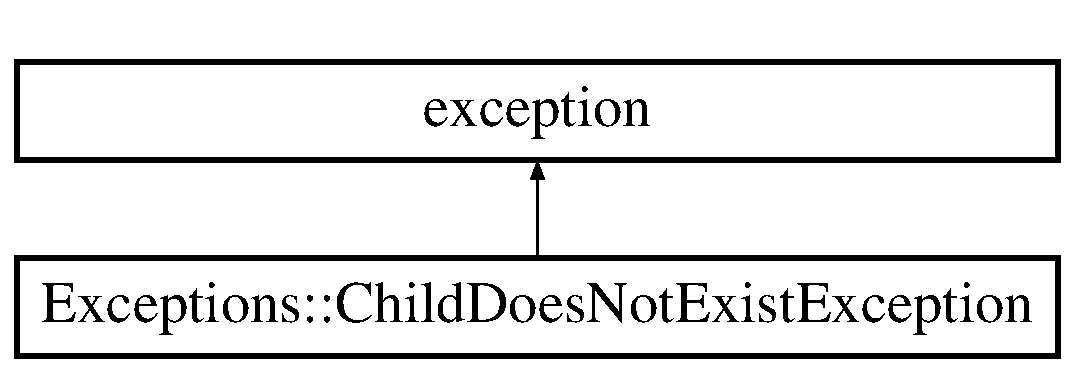
\includegraphics[height=2.000000cm]{class_exceptions_1_1_child_does_not_exist_exception}
\end{center}
\end{figure}
\subsection*{Public Member Functions}
\begin{DoxyCompactItemize}
\item 
\hyperlink{class_exceptions_1_1_child_does_not_exist_exception_a5c7450ff322fb5f8eb3221744ef72500}{Child\+Does\+Not\+Exist\+Exception} ()
\item 
virtual const char $\ast$ \hyperlink{class_exceptions_1_1_child_does_not_exist_exception_aaa7854075d3e72e6eb294d1c25759b13}{what} () const   throw ()
\end{DoxyCompactItemize}


\subsection{Constructor \& Destructor Documentation}
\hypertarget{class_exceptions_1_1_child_does_not_exist_exception_a5c7450ff322fb5f8eb3221744ef72500}{}\index{Exceptions\+::\+Child\+Does\+Not\+Exist\+Exception@{Exceptions\+::\+Child\+Does\+Not\+Exist\+Exception}!Child\+Does\+Not\+Exist\+Exception@{Child\+Does\+Not\+Exist\+Exception}}
\index{Child\+Does\+Not\+Exist\+Exception@{Child\+Does\+Not\+Exist\+Exception}!Exceptions\+::\+Child\+Does\+Not\+Exist\+Exception@{Exceptions\+::\+Child\+Does\+Not\+Exist\+Exception}}
\subsubsection[{Child\+Does\+Not\+Exist\+Exception}]{\setlength{\rightskip}{0pt plus 5cm}Exceptions\+::\+Child\+Does\+Not\+Exist\+Exception\+::\+Child\+Does\+Not\+Exist\+Exception (
\begin{DoxyParamCaption}
{}
\end{DoxyParamCaption}
)\hspace{0.3cm}{\ttfamily [inline]}}\label{class_exceptions_1_1_child_does_not_exist_exception_a5c7450ff322fb5f8eb3221744ef72500}


\subsection{Member Function Documentation}
\hypertarget{class_exceptions_1_1_child_does_not_exist_exception_aaa7854075d3e72e6eb294d1c25759b13}{}\index{Exceptions\+::\+Child\+Does\+Not\+Exist\+Exception@{Exceptions\+::\+Child\+Does\+Not\+Exist\+Exception}!what@{what}}
\index{what@{what}!Exceptions\+::\+Child\+Does\+Not\+Exist\+Exception@{Exceptions\+::\+Child\+Does\+Not\+Exist\+Exception}}
\subsubsection[{what}]{\setlength{\rightskip}{0pt plus 5cm}virtual const char$\ast$ Exceptions\+::\+Child\+Does\+Not\+Exist\+Exception\+::what (
\begin{DoxyParamCaption}
{}
\end{DoxyParamCaption}
) const throw  ) \hspace{0.3cm}{\ttfamily [inline]}, {\ttfamily [virtual]}}\label{class_exceptions_1_1_child_does_not_exist_exception_aaa7854075d3e72e6eb294d1c25759b13}


The documentation for this class was generated from the following file\+:\begin{DoxyCompactItemize}
\item 
src/exceptions/\hyperlink{child__does__not__exist__exception_8h}{child\+\_\+does\+\_\+not\+\_\+exist\+\_\+exception.\+h}\end{DoxyCompactItemize}

\hypertarget{class_component}{}\section{Component Class Reference}
\label{class_component}\index{Component@{Component}}


{\ttfamily \#include $<$component.\+h$>$}

Inheritance diagram for Component\+:\begin{figure}[H]
\begin{center}
\leavevmode
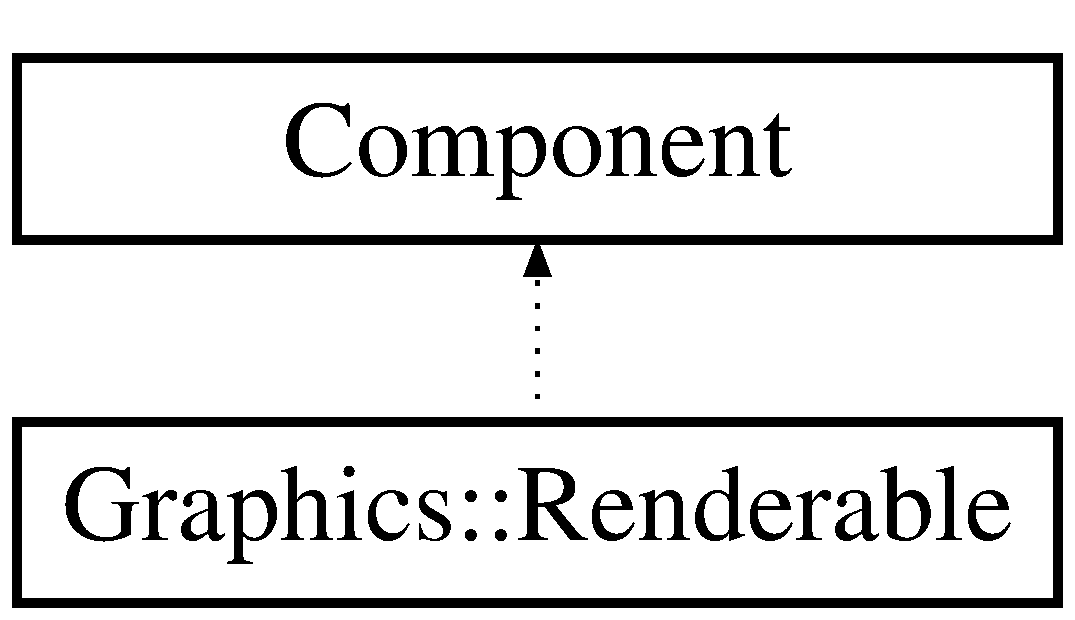
\includegraphics[height=4.000000cm]{class_component}
\end{center}
\end{figure}
\subsection*{Public Member Functions}
\begin{DoxyCompactItemize}
\item 
\hyperlink{class_component_a8775db6d1a2c1afc2e77cd3c8f39da6f}{Component} ()
\item 
virtual void \hyperlink{class_component_a4a528a8790dbc141ffd0aba638b6dcc4}{on\+Start} ()=0
\item 
virtual const bool \hyperlink{class_component_a8be284fccf4e97cee6705bd2d8f3705e}{on\+Update} (const double delta)=0
\item 
virtual void \hyperlink{class_component_a2b198f27162a6caf63917e304295f892}{on\+Destroy} ()=0
\item 
void \hyperlink{class_component_a8842d3ce36b584a3e7d0cb7734232812}{set\+Transform} (std\+::shared\+\_\+ptr$<$ \hyperlink{class_transform}{Transform} $>$ \hyperlink{class_component_a02b1c70de1d9e2c6499dff349da1b0ff}{transform})
\item 
std\+::shared\+\_\+ptr$<$ \hyperlink{class_transform}{Transform} $>$ \hyperlink{class_component_a94dfec102ece6b669176f0609b0a5497}{get\+Transform} () const noexcept
\item 
virtual \hyperlink{class_component_a2e9aa4348314d981f05f67397ad2f872}{$\sim$\+Component} ()
\end{DoxyCompactItemize}
\subsection*{Protected Attributes}
\begin{DoxyCompactItemize}
\item 
std\+::shared\+\_\+ptr$<$ \hyperlink{class_transform}{Transform} $>$ \hyperlink{class_component_a02b1c70de1d9e2c6499dff349da1b0ff}{transform}
\end{DoxyCompactItemize}


\subsection{Constructor \& Destructor Documentation}
\hypertarget{class_component_a8775db6d1a2c1afc2e77cd3c8f39da6f}{}\index{Component@{Component}!Component@{Component}}
\index{Component@{Component}!Component@{Component}}
\subsubsection[{Component}]{\setlength{\rightskip}{0pt plus 5cm}Component\+::\+Component (
\begin{DoxyParamCaption}
{}
\end{DoxyParamCaption}
)}\label{class_component_a8775db6d1a2c1afc2e77cd3c8f39da6f}
\hypertarget{class_component_a2e9aa4348314d981f05f67397ad2f872}{}\index{Component@{Component}!````~Component@{$\sim$\+Component}}
\index{````~Component@{$\sim$\+Component}!Component@{Component}}
\subsubsection[{$\sim$\+Component}]{\setlength{\rightskip}{0pt plus 5cm}virtual Component\+::$\sim$\+Component (
\begin{DoxyParamCaption}
{}
\end{DoxyParamCaption}
)\hspace{0.3cm}{\ttfamily [inline]}, {\ttfamily [virtual]}}\label{class_component_a2e9aa4348314d981f05f67397ad2f872}


\subsection{Member Function Documentation}
\hypertarget{class_component_a94dfec102ece6b669176f0609b0a5497}{}\index{Component@{Component}!get\+Transform@{get\+Transform}}
\index{get\+Transform@{get\+Transform}!Component@{Component}}
\subsubsection[{get\+Transform}]{\setlength{\rightskip}{0pt plus 5cm}std\+::shared\+\_\+ptr$<$ {\bf Transform} $>$ Component\+::get\+Transform (
\begin{DoxyParamCaption}
{}
\end{DoxyParamCaption}
) const\hspace{0.3cm}{\ttfamily [noexcept]}}\label{class_component_a94dfec102ece6b669176f0609b0a5497}
\hypertarget{class_component_a2b198f27162a6caf63917e304295f892}{}\index{Component@{Component}!on\+Destroy@{on\+Destroy}}
\index{on\+Destroy@{on\+Destroy}!Component@{Component}}
\subsubsection[{on\+Destroy}]{\setlength{\rightskip}{0pt plus 5cm}virtual void Component\+::on\+Destroy (
\begin{DoxyParamCaption}
{}
\end{DoxyParamCaption}
)\hspace{0.3cm}{\ttfamily [pure virtual]}}\label{class_component_a2b198f27162a6caf63917e304295f892}


Implemented in \hyperlink{class_graphics_1_1_renderable_a6e20996de55215db7ffae2792aaaa88e}{Graphics\+::\+Renderable}, \hyperlink{class_graphics_1_1_camera_a9d8ca67cbd7a586915fc6cfd303406de}{Graphics\+::\+Camera}, \hyperlink{class_graphics_1_1_light_a7d4ce913fcb79612a90937ae75b3ff2e}{Graphics\+::\+Light}, \hyperlink{class_graphics_1_1_animated_tile_a9781b9b256a666a123fd2c050adb5118}{Graphics\+::\+Animated\+Tile}, and \hyperlink{class_graphics_1_1_tile_a28f5bdfa2fc61b292dda7ec15316b981}{Graphics\+::\+Tile}.

\hypertarget{class_component_a4a528a8790dbc141ffd0aba638b6dcc4}{}\index{Component@{Component}!on\+Start@{on\+Start}}
\index{on\+Start@{on\+Start}!Component@{Component}}
\subsubsection[{on\+Start}]{\setlength{\rightskip}{0pt plus 5cm}virtual void Component\+::on\+Start (
\begin{DoxyParamCaption}
{}
\end{DoxyParamCaption}
)\hspace{0.3cm}{\ttfamily [pure virtual]}}\label{class_component_a4a528a8790dbc141ffd0aba638b6dcc4}


Implemented in \hyperlink{class_graphics_1_1_renderable_a7433551970cd25e0241a4a5bb756ba50}{Graphics\+::\+Renderable}, \hyperlink{class_graphics_1_1_camera_a37edadff497ff3966c2190b876bfe236}{Graphics\+::\+Camera}, \hyperlink{class_graphics_1_1_light_aa8ff320220d375edddae38daec0b3672}{Graphics\+::\+Light}, and \hyperlink{class_graphics_1_1_animated_tile_ad82e39321244cc2e06ee3df527473aba}{Graphics\+::\+Animated\+Tile}.

\hypertarget{class_component_a8be284fccf4e97cee6705bd2d8f3705e}{}\index{Component@{Component}!on\+Update@{on\+Update}}
\index{on\+Update@{on\+Update}!Component@{Component}}
\subsubsection[{on\+Update}]{\setlength{\rightskip}{0pt plus 5cm}virtual const bool Component\+::on\+Update (
\begin{DoxyParamCaption}
\item[{const double}]{delta}
\end{DoxyParamCaption}
)\hspace{0.3cm}{\ttfamily [pure virtual]}}\label{class_component_a8be284fccf4e97cee6705bd2d8f3705e}


Implemented in \hyperlink{class_graphics_1_1_renderable_a7d0e820c55cb7f5c552aa0c1e846db76}{Graphics\+::\+Renderable}, \hyperlink{class_graphics_1_1_camera_a0bfccb5623342c93f69b408937b87374}{Graphics\+::\+Camera}, \hyperlink{class_graphics_1_1_light_ab208fc670894a75038b0e74a75816b21}{Graphics\+::\+Light}, \hyperlink{class_graphics_1_1_animated_tile_a2c6f7cd3866cad84b73ea5da8b92b76e}{Graphics\+::\+Animated\+Tile}, and \hyperlink{class_graphics_1_1_tile_a0311b1d9548f6badc9e81820b110cbb4}{Graphics\+::\+Tile}.

\hypertarget{class_component_a8842d3ce36b584a3e7d0cb7734232812}{}\index{Component@{Component}!set\+Transform@{set\+Transform}}
\index{set\+Transform@{set\+Transform}!Component@{Component}}
\subsubsection[{set\+Transform}]{\setlength{\rightskip}{0pt plus 5cm}void Component\+::set\+Transform (
\begin{DoxyParamCaption}
\item[{std\+::shared\+\_\+ptr$<$ {\bf Transform} $>$}]{transform}
\end{DoxyParamCaption}
)}\label{class_component_a8842d3ce36b584a3e7d0cb7734232812}


\subsection{Member Data Documentation}
\hypertarget{class_component_a02b1c70de1d9e2c6499dff349da1b0ff}{}\index{Component@{Component}!transform@{transform}}
\index{transform@{transform}!Component@{Component}}
\subsubsection[{transform}]{\setlength{\rightskip}{0pt plus 5cm}std\+::shared\+\_\+ptr$<${\bf Transform}$>$ Component\+::transform\hspace{0.3cm}{\ttfamily [protected]}}\label{class_component_a02b1c70de1d9e2c6499dff349da1b0ff}


The documentation for this class was generated from the following files\+:\begin{DoxyCompactItemize}
\item 
src/\hyperlink{component_8h}{component.\+h}\item 
src/\hyperlink{component_8cpp}{component.\+cpp}\end{DoxyCompactItemize}

\hypertarget{class_utility_1_1_config_manager}{}\section{Utility\+:\+:Config\+Manager Class Reference}
\label{class_utility_1_1_config_manager}\index{Utility\+::\+Config\+Manager@{Utility\+::\+Config\+Manager}}


{\ttfamily \#include $<$config\+\_\+manager.\+h$>$}

\subsection*{Public Member Functions}
\begin{DoxyCompactItemize}
\item 
\hyperlink{class_utility_1_1_config_manager_a228593ff6e819ca2bbd95d6e09088b20}{Config\+Manager} ()
\item 
const bool \hyperlink{class_utility_1_1_config_manager_a61ba82f3a3283b3c8ce32f9711d251df}{load\+Config} (const std\+::string \&file\+\_\+path)
\item 
const int \hyperlink{class_utility_1_1_config_manager_a028532027515473be914ddd4a27f4c93}{get\+Int} (const std\+::string \&key)
\item 
const unsigned int \hyperlink{class_utility_1_1_config_manager_acfbc4d2fd290ba15c044bc143fc137a4}{get\+Unsigned\+Int} (const std\+::string \&key)
\item 
const std\+::string \hyperlink{class_utility_1_1_config_manager_a1cab9c879509bd136a1335881733d292}{get\+String} (const std\+::string \&key)
\item 
const float \hyperlink{class_utility_1_1_config_manager_a2f94493014047e06503fb1a42b2ff18d}{get\+Float} (const std\+::string \&key)
\item 
const double \hyperlink{class_utility_1_1_config_manager_a070db02341204507c39799ce330f0446}{get\+Double} (const std\+::string \&key)
\item 
const bool \hyperlink{class_utility_1_1_config_manager_af0d3c6da273b45bcb7580a0a5ae609ef}{get\+Bool} (const std\+::string \&key)
\end{DoxyCompactItemize}
\subsection*{Private Attributes}
\begin{DoxyCompactItemize}
\item 
Json\+::\+Value \hyperlink{class_utility_1_1_config_manager_a265dc71bf65917984c7c63e0ad847c2f}{config\+\_\+handle}
\end{DoxyCompactItemize}


\subsection{Constructor \& Destructor Documentation}
\hypertarget{class_utility_1_1_config_manager_a228593ff6e819ca2bbd95d6e09088b20}{}\index{Utility\+::\+Config\+Manager@{Utility\+::\+Config\+Manager}!Config\+Manager@{Config\+Manager}}
\index{Config\+Manager@{Config\+Manager}!Utility\+::\+Config\+Manager@{Utility\+::\+Config\+Manager}}
\subsubsection[{Config\+Manager}]{\setlength{\rightskip}{0pt plus 5cm}Utility\+::\+Config\+Manager\+::\+Config\+Manager (
\begin{DoxyParamCaption}
{}
\end{DoxyParamCaption}
)}\label{class_utility_1_1_config_manager_a228593ff6e819ca2bbd95d6e09088b20}


\subsection{Member Function Documentation}
\hypertarget{class_utility_1_1_config_manager_af0d3c6da273b45bcb7580a0a5ae609ef}{}\index{Utility\+::\+Config\+Manager@{Utility\+::\+Config\+Manager}!get\+Bool@{get\+Bool}}
\index{get\+Bool@{get\+Bool}!Utility\+::\+Config\+Manager@{Utility\+::\+Config\+Manager}}
\subsubsection[{get\+Bool}]{\setlength{\rightskip}{0pt plus 5cm}const bool Utility\+::\+Config\+Manager\+::get\+Bool (
\begin{DoxyParamCaption}
\item[{const std\+::string \&}]{key}
\end{DoxyParamCaption}
)}\label{class_utility_1_1_config_manager_af0d3c6da273b45bcb7580a0a5ae609ef}
\hypertarget{class_utility_1_1_config_manager_a070db02341204507c39799ce330f0446}{}\index{Utility\+::\+Config\+Manager@{Utility\+::\+Config\+Manager}!get\+Double@{get\+Double}}
\index{get\+Double@{get\+Double}!Utility\+::\+Config\+Manager@{Utility\+::\+Config\+Manager}}
\subsubsection[{get\+Double}]{\setlength{\rightskip}{0pt plus 5cm}const double Utility\+::\+Config\+Manager\+::get\+Double (
\begin{DoxyParamCaption}
\item[{const std\+::string \&}]{key}
\end{DoxyParamCaption}
)}\label{class_utility_1_1_config_manager_a070db02341204507c39799ce330f0446}
\hypertarget{class_utility_1_1_config_manager_a2f94493014047e06503fb1a42b2ff18d}{}\index{Utility\+::\+Config\+Manager@{Utility\+::\+Config\+Manager}!get\+Float@{get\+Float}}
\index{get\+Float@{get\+Float}!Utility\+::\+Config\+Manager@{Utility\+::\+Config\+Manager}}
\subsubsection[{get\+Float}]{\setlength{\rightskip}{0pt plus 5cm}const float Utility\+::\+Config\+Manager\+::get\+Float (
\begin{DoxyParamCaption}
\item[{const std\+::string \&}]{key}
\end{DoxyParamCaption}
)}\label{class_utility_1_1_config_manager_a2f94493014047e06503fb1a42b2ff18d}
\hypertarget{class_utility_1_1_config_manager_a028532027515473be914ddd4a27f4c93}{}\index{Utility\+::\+Config\+Manager@{Utility\+::\+Config\+Manager}!get\+Int@{get\+Int}}
\index{get\+Int@{get\+Int}!Utility\+::\+Config\+Manager@{Utility\+::\+Config\+Manager}}
\subsubsection[{get\+Int}]{\setlength{\rightskip}{0pt plus 5cm}const int Utility\+::\+Config\+Manager\+::get\+Int (
\begin{DoxyParamCaption}
\item[{const std\+::string \&}]{key}
\end{DoxyParamCaption}
)}\label{class_utility_1_1_config_manager_a028532027515473be914ddd4a27f4c93}
\hypertarget{class_utility_1_1_config_manager_a1cab9c879509bd136a1335881733d292}{}\index{Utility\+::\+Config\+Manager@{Utility\+::\+Config\+Manager}!get\+String@{get\+String}}
\index{get\+String@{get\+String}!Utility\+::\+Config\+Manager@{Utility\+::\+Config\+Manager}}
\subsubsection[{get\+String}]{\setlength{\rightskip}{0pt plus 5cm}const std\+::string Utility\+::\+Config\+Manager\+::get\+String (
\begin{DoxyParamCaption}
\item[{const std\+::string \&}]{key}
\end{DoxyParamCaption}
)}\label{class_utility_1_1_config_manager_a1cab9c879509bd136a1335881733d292}
\hypertarget{class_utility_1_1_config_manager_acfbc4d2fd290ba15c044bc143fc137a4}{}\index{Utility\+::\+Config\+Manager@{Utility\+::\+Config\+Manager}!get\+Unsigned\+Int@{get\+Unsigned\+Int}}
\index{get\+Unsigned\+Int@{get\+Unsigned\+Int}!Utility\+::\+Config\+Manager@{Utility\+::\+Config\+Manager}}
\subsubsection[{get\+Unsigned\+Int}]{\setlength{\rightskip}{0pt plus 5cm}const unsigned int Utility\+::\+Config\+Manager\+::get\+Unsigned\+Int (
\begin{DoxyParamCaption}
\item[{const std\+::string \&}]{key}
\end{DoxyParamCaption}
)}\label{class_utility_1_1_config_manager_acfbc4d2fd290ba15c044bc143fc137a4}
\hypertarget{class_utility_1_1_config_manager_a61ba82f3a3283b3c8ce32f9711d251df}{}\index{Utility\+::\+Config\+Manager@{Utility\+::\+Config\+Manager}!load\+Config@{load\+Config}}
\index{load\+Config@{load\+Config}!Utility\+::\+Config\+Manager@{Utility\+::\+Config\+Manager}}
\subsubsection[{load\+Config}]{\setlength{\rightskip}{0pt plus 5cm}const bool Utility\+::\+Config\+Manager\+::load\+Config (
\begin{DoxyParamCaption}
\item[{const std\+::string \&}]{file\+\_\+path}
\end{DoxyParamCaption}
)}\label{class_utility_1_1_config_manager_a61ba82f3a3283b3c8ce32f9711d251df}


\subsection{Member Data Documentation}
\hypertarget{class_utility_1_1_config_manager_a265dc71bf65917984c7c63e0ad847c2f}{}\index{Utility\+::\+Config\+Manager@{Utility\+::\+Config\+Manager}!config\+\_\+handle@{config\+\_\+handle}}
\index{config\+\_\+handle@{config\+\_\+handle}!Utility\+::\+Config\+Manager@{Utility\+::\+Config\+Manager}}
\subsubsection[{config\+\_\+handle}]{\setlength{\rightskip}{0pt plus 5cm}Json\+::\+Value Utility\+::\+Config\+Manager\+::config\+\_\+handle\hspace{0.3cm}{\ttfamily [private]}}\label{class_utility_1_1_config_manager_a265dc71bf65917984c7c63e0ad847c2f}


The documentation for this class was generated from the following files\+:\begin{DoxyCompactItemize}
\item 
src/utility/\hyperlink{config__manager_8h}{config\+\_\+manager.\+h}\item 
src/utility/\hyperlink{config__manager_8cpp}{config\+\_\+manager.\+cpp}\end{DoxyCompactItemize}

\hypertarget{class_exceptions_1_1_config_not_loaded_exception}{}\section{Exceptions\+:\+:Config\+Not\+Loaded\+Exception Class Reference}
\label{class_exceptions_1_1_config_not_loaded_exception}\index{Exceptions\+::\+Config\+Not\+Loaded\+Exception@{Exceptions\+::\+Config\+Not\+Loaded\+Exception}}


{\ttfamily \#include $<$config\+\_\+not\+\_\+loaded\+\_\+exception.\+h$>$}

Inheritance diagram for Exceptions\+:\+:Config\+Not\+Loaded\+Exception\+:\begin{figure}[H]
\begin{center}
\leavevmode
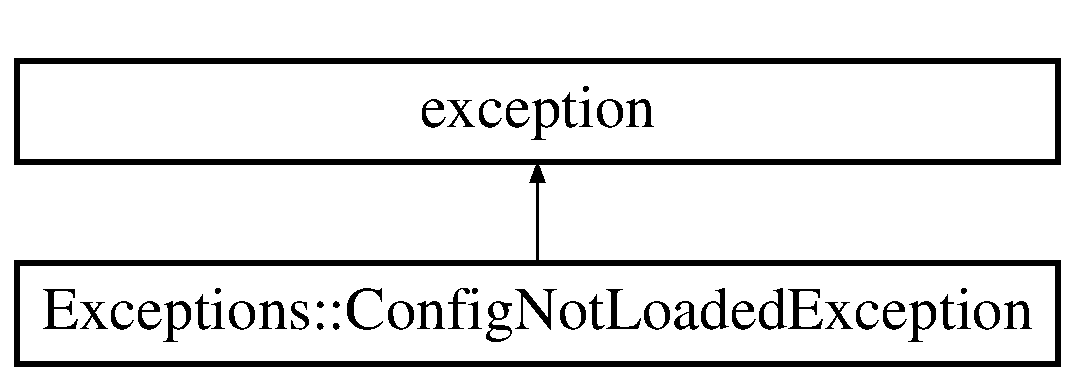
\includegraphics[height=2.000000cm]{class_exceptions_1_1_config_not_loaded_exception}
\end{center}
\end{figure}
\subsection*{Public Member Functions}
\begin{DoxyCompactItemize}
\item 
\hyperlink{class_exceptions_1_1_config_not_loaded_exception_a69309ae87ed770a5ff884173752bd763}{Config\+Not\+Loaded\+Exception} ()
\item 
virtual const char $\ast$ \hyperlink{class_exceptions_1_1_config_not_loaded_exception_aede41d33e660a0eb101c03dc81a7c101}{what} () const   throw ()
\end{DoxyCompactItemize}


\subsection{Constructor \& Destructor Documentation}
\hypertarget{class_exceptions_1_1_config_not_loaded_exception_a69309ae87ed770a5ff884173752bd763}{}\index{Exceptions\+::\+Config\+Not\+Loaded\+Exception@{Exceptions\+::\+Config\+Not\+Loaded\+Exception}!Config\+Not\+Loaded\+Exception@{Config\+Not\+Loaded\+Exception}}
\index{Config\+Not\+Loaded\+Exception@{Config\+Not\+Loaded\+Exception}!Exceptions\+::\+Config\+Not\+Loaded\+Exception@{Exceptions\+::\+Config\+Not\+Loaded\+Exception}}
\subsubsection[{Config\+Not\+Loaded\+Exception}]{\setlength{\rightskip}{0pt plus 5cm}Exceptions\+::\+Config\+Not\+Loaded\+Exception\+::\+Config\+Not\+Loaded\+Exception (
\begin{DoxyParamCaption}
{}
\end{DoxyParamCaption}
)\hspace{0.3cm}{\ttfamily [inline]}}\label{class_exceptions_1_1_config_not_loaded_exception_a69309ae87ed770a5ff884173752bd763}


\subsection{Member Function Documentation}
\hypertarget{class_exceptions_1_1_config_not_loaded_exception_aede41d33e660a0eb101c03dc81a7c101}{}\index{Exceptions\+::\+Config\+Not\+Loaded\+Exception@{Exceptions\+::\+Config\+Not\+Loaded\+Exception}!what@{what}}
\index{what@{what}!Exceptions\+::\+Config\+Not\+Loaded\+Exception@{Exceptions\+::\+Config\+Not\+Loaded\+Exception}}
\subsubsection[{what}]{\setlength{\rightskip}{0pt plus 5cm}virtual const char$\ast$ Exceptions\+::\+Config\+Not\+Loaded\+Exception\+::what (
\begin{DoxyParamCaption}
{}
\end{DoxyParamCaption}
) const throw  ) \hspace{0.3cm}{\ttfamily [inline]}, {\ttfamily [virtual]}}\label{class_exceptions_1_1_config_not_loaded_exception_aede41d33e660a0eb101c03dc81a7c101}


The documentation for this class was generated from the following file\+:\begin{DoxyCompactItemize}
\item 
src/exceptions/\hyperlink{config__not__loaded__exception_8h}{config\+\_\+not\+\_\+loaded\+\_\+exception.\+h}\end{DoxyCompactItemize}

\hypertarget{class_input_1_1_cursor_enter_event}{}\section{Input\+:\+:Cursor\+Enter\+Event Class Reference}
\label{class_input_1_1_cursor_enter_event}\index{Input\+::\+Cursor\+Enter\+Event@{Input\+::\+Cursor\+Enter\+Event}}


{\ttfamily \#include $<$cursor\+\_\+enter\+\_\+event.\+h$>$}

Inheritance diagram for Input\+:\+:Cursor\+Enter\+Event\+:\begin{figure}[H]
\begin{center}
\leavevmode
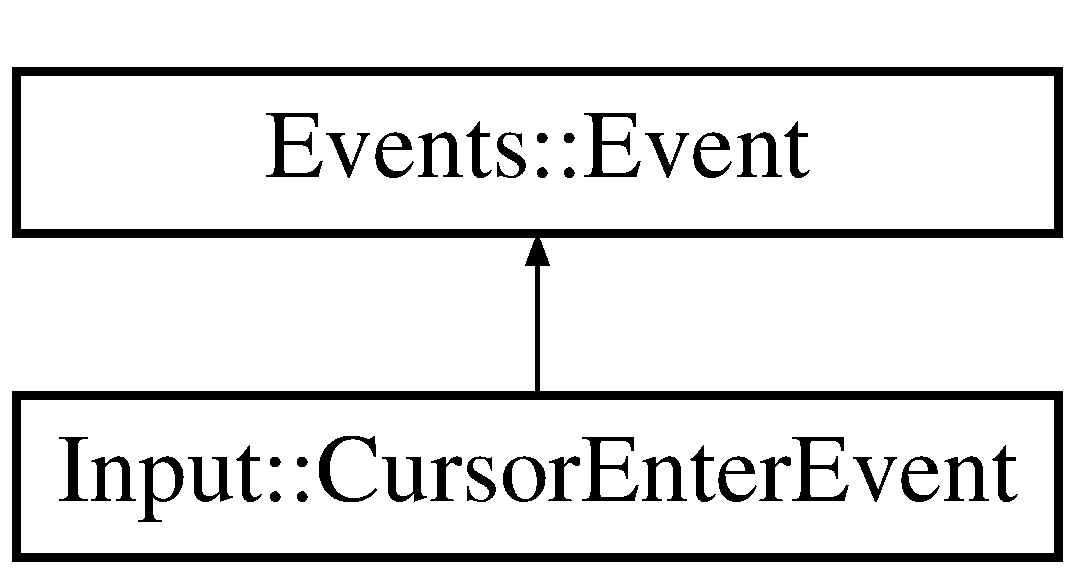
\includegraphics[height=2.000000cm]{class_input_1_1_cursor_enter_event}
\end{center}
\end{figure}
\subsection*{Public Member Functions}
\begin{DoxyCompactItemize}
\item 
\hyperlink{class_input_1_1_cursor_enter_event_a667aae38786f7d6d0c2a2ad4e0de01da}{Cursor\+Enter\+Event} ()
\end{DoxyCompactItemize}


\subsection{Constructor \& Destructor Documentation}
\hypertarget{class_input_1_1_cursor_enter_event_a667aae38786f7d6d0c2a2ad4e0de01da}{}\index{Input\+::\+Cursor\+Enter\+Event@{Input\+::\+Cursor\+Enter\+Event}!Cursor\+Enter\+Event@{Cursor\+Enter\+Event}}
\index{Cursor\+Enter\+Event@{Cursor\+Enter\+Event}!Input\+::\+Cursor\+Enter\+Event@{Input\+::\+Cursor\+Enter\+Event}}
\subsubsection[{Cursor\+Enter\+Event}]{\setlength{\rightskip}{0pt plus 5cm}Input\+::\+Cursor\+Enter\+Event\+::\+Cursor\+Enter\+Event (
\begin{DoxyParamCaption}
{}
\end{DoxyParamCaption}
)\hspace{0.3cm}{\ttfamily [inline]}}\label{class_input_1_1_cursor_enter_event_a667aae38786f7d6d0c2a2ad4e0de01da}


The documentation for this class was generated from the following file\+:\begin{DoxyCompactItemize}
\item 
src/input/\hyperlink{cursor__enter__event_8h}{cursor\+\_\+enter\+\_\+event.\+h}\end{DoxyCompactItemize}

\hypertarget{class_input_1_1_cursor_leave_event}{}\section{Input\+:\+:Cursor\+Leave\+Event Class Reference}
\label{class_input_1_1_cursor_leave_event}\index{Input\+::\+Cursor\+Leave\+Event@{Input\+::\+Cursor\+Leave\+Event}}


{\ttfamily \#include $<$cursor\+\_\+leave\+\_\+event.\+h$>$}

Inheritance diagram for Input\+:\+:Cursor\+Leave\+Event\+:\begin{figure}[H]
\begin{center}
\leavevmode
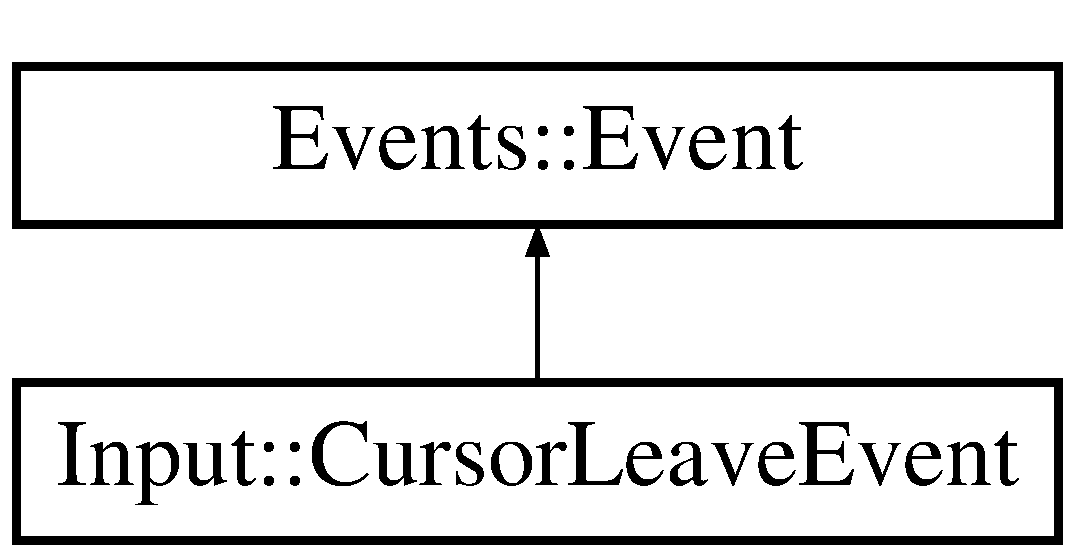
\includegraphics[height=2.000000cm]{class_input_1_1_cursor_leave_event}
\end{center}
\end{figure}
\subsection*{Public Member Functions}
\begin{DoxyCompactItemize}
\item 
\hyperlink{class_input_1_1_cursor_leave_event_aeed68b4a22c6f5944a70799728d0e439}{Cursor\+Leave\+Event} ()
\end{DoxyCompactItemize}


\subsection{Constructor \& Destructor Documentation}
\hypertarget{class_input_1_1_cursor_leave_event_aeed68b4a22c6f5944a70799728d0e439}{}\index{Input\+::\+Cursor\+Leave\+Event@{Input\+::\+Cursor\+Leave\+Event}!Cursor\+Leave\+Event@{Cursor\+Leave\+Event}}
\index{Cursor\+Leave\+Event@{Cursor\+Leave\+Event}!Input\+::\+Cursor\+Leave\+Event@{Input\+::\+Cursor\+Leave\+Event}}
\subsubsection[{Cursor\+Leave\+Event}]{\setlength{\rightskip}{0pt plus 5cm}Input\+::\+Cursor\+Leave\+Event\+::\+Cursor\+Leave\+Event (
\begin{DoxyParamCaption}
{}
\end{DoxyParamCaption}
)\hspace{0.3cm}{\ttfamily [inline]}}\label{class_input_1_1_cursor_leave_event_aeed68b4a22c6f5944a70799728d0e439}


The documentation for this class was generated from the following file\+:\begin{DoxyCompactItemize}
\item 
src/input/\hyperlink{cursor__leave__event_8h}{cursor\+\_\+leave\+\_\+event.\+h}\end{DoxyCompactItemize}

\hypertarget{class_entity}{}\section{Entity Class Reference}
\label{class_entity}\index{Entity@{Entity}}


{\ttfamily \#include $<$entity.\+h$>$}

Inheritance diagram for Entity\+:\begin{figure}[H]
\begin{center}
\leavevmode
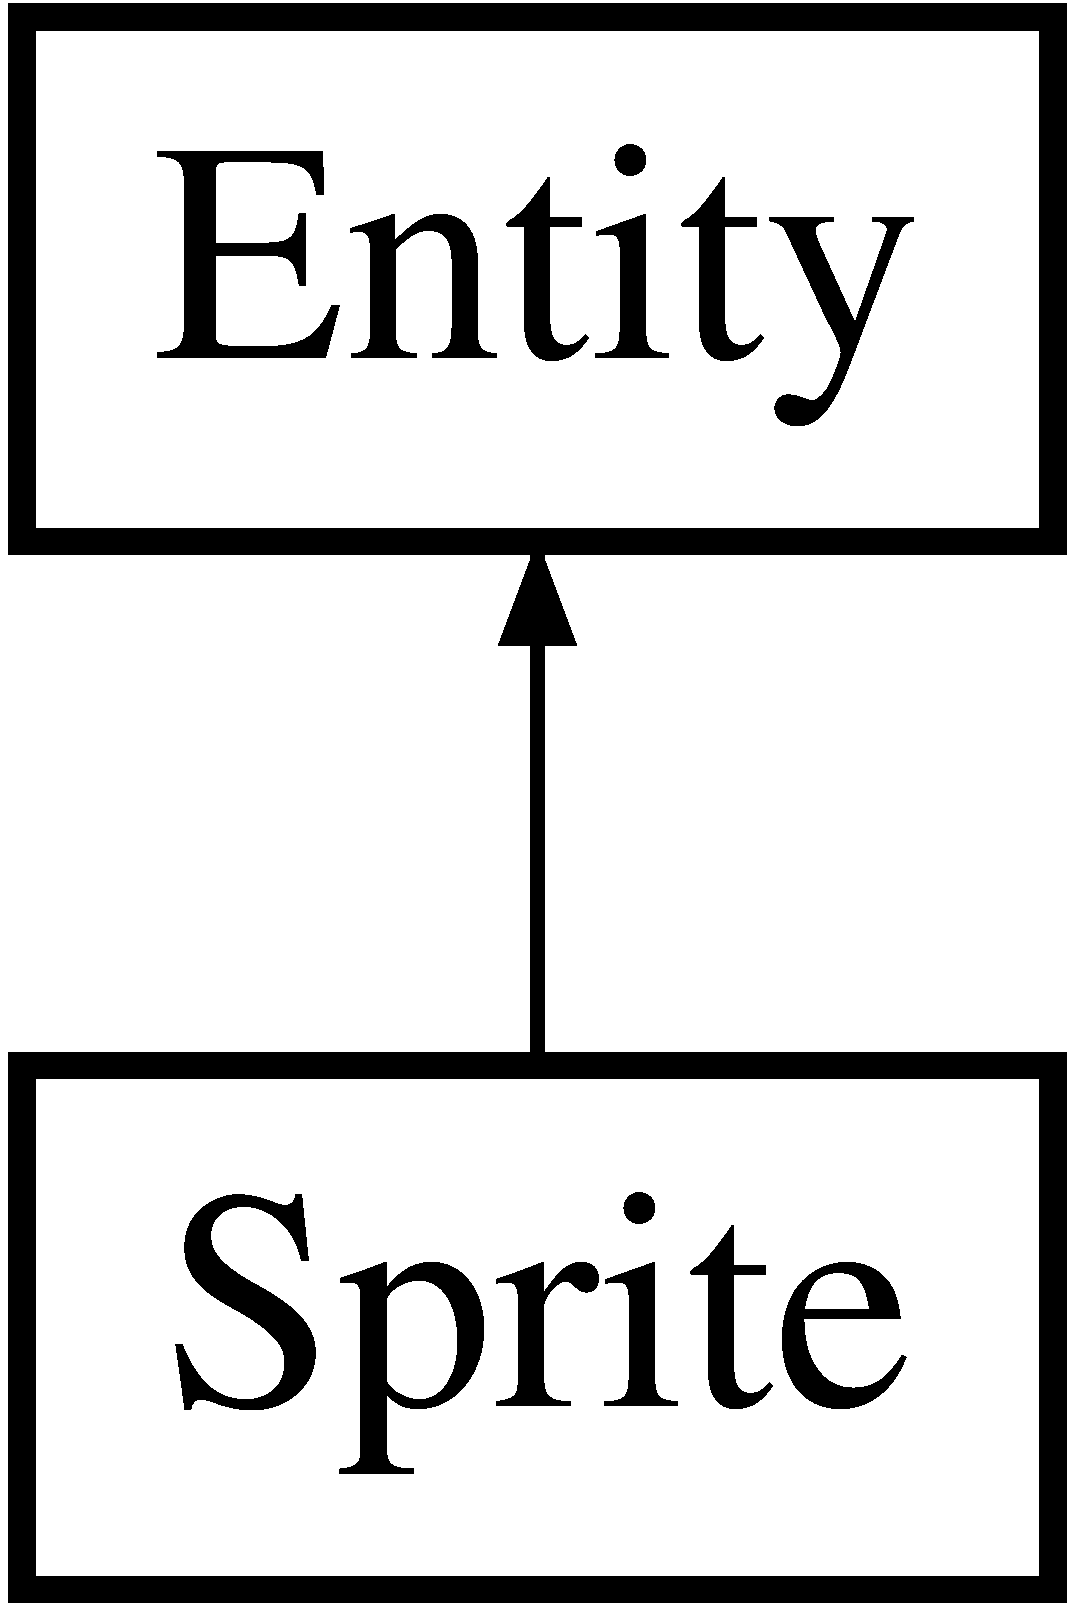
\includegraphics[height=2.000000cm]{class_entity}
\end{center}
\end{figure}
\subsection*{Public Member Functions}
\begin{DoxyCompactItemize}
\item 
\hyperlink{class_entity_a980f368aa07ce358583982821533a54a}{Entity} ()
\item 
void \hyperlink{class_entity_a1e04612ca60083490443ff1dff92b3fe}{add\+Component} (std\+::shared\+\_\+ptr$<$ \hyperlink{class_component}{Component} $>$ component)
\item 
void \hyperlink{class_entity_a6c736e11abe151f3997be250e25935d6}{remove\+Component} (std\+::shared\+\_\+ptr$<$ \hyperlink{class_component}{Component} $>$ component)
\item 
std\+::shared\+\_\+ptr$<$ \hyperlink{class_transform}{Transform} $>$ \hyperlink{class_entity_a3fc75182569e1dafabffdb1920c16073}{get\+Transform} () const noexcept
\item 
virtual void \hyperlink{class_entity_afe788ab09347ad97ca39af8133a55589}{on\+Start} ()
\item 
virtual void \hyperlink{class_entity_a43745870ac080aea60c717611c10145d}{on\+Update} (const float delta)
\item 
virtual void \hyperlink{class_entity_ae791185bd4921dc4e8b7fed92f6553e6}{on\+Stop} ()
\item 
virtual void \hyperlink{class_entity_a6db576733100dea6173fa5818ff11f10}{on\+Destroy} ()
\end{DoxyCompactItemize}
\subsection*{Protected Attributes}
\begin{DoxyCompactItemize}
\item 
std\+::list$<$ std\+::shared\+\_\+ptr$<$ \hyperlink{class_component}{Component} $>$ $>$ \hyperlink{class_entity_a91f8301ced2daaaed904292bd34460dd}{components}
\end{DoxyCompactItemize}
\subsection*{Private Attributes}
\begin{DoxyCompactItemize}
\item 
std\+::shared\+\_\+ptr$<$ \hyperlink{class_transform}{Transform} $>$ \hyperlink{class_entity_ab2b82c9846ff3adc81074b3fa61f143a}{transform}
\end{DoxyCompactItemize}


\subsection{Constructor \& Destructor Documentation}
\hypertarget{class_entity_a980f368aa07ce358583982821533a54a}{}\index{Entity@{Entity}!Entity@{Entity}}
\index{Entity@{Entity}!Entity@{Entity}}
\subsubsection[{Entity}]{\setlength{\rightskip}{0pt plus 5cm}Entity\+::\+Entity (
\begin{DoxyParamCaption}
{}
\end{DoxyParamCaption}
)}\label{class_entity_a980f368aa07ce358583982821533a54a}


\subsection{Member Function Documentation}
\hypertarget{class_entity_a1e04612ca60083490443ff1dff92b3fe}{}\index{Entity@{Entity}!add\+Component@{add\+Component}}
\index{add\+Component@{add\+Component}!Entity@{Entity}}
\subsubsection[{add\+Component}]{\setlength{\rightskip}{0pt plus 5cm}void Entity\+::add\+Component (
\begin{DoxyParamCaption}
\item[{std\+::shared\+\_\+ptr$<$ {\bf Component} $>$}]{component}
\end{DoxyParamCaption}
)}\label{class_entity_a1e04612ca60083490443ff1dff92b3fe}
\hypertarget{class_entity_a3fc75182569e1dafabffdb1920c16073}{}\index{Entity@{Entity}!get\+Transform@{get\+Transform}}
\index{get\+Transform@{get\+Transform}!Entity@{Entity}}
\subsubsection[{get\+Transform}]{\setlength{\rightskip}{0pt plus 5cm}std\+::shared\+\_\+ptr$<$ {\bf Transform} $>$ Entity\+::get\+Transform (
\begin{DoxyParamCaption}
{}
\end{DoxyParamCaption}
) const\hspace{0.3cm}{\ttfamily [noexcept]}}\label{class_entity_a3fc75182569e1dafabffdb1920c16073}
\hypertarget{class_entity_a6db576733100dea6173fa5818ff11f10}{}\index{Entity@{Entity}!on\+Destroy@{on\+Destroy}}
\index{on\+Destroy@{on\+Destroy}!Entity@{Entity}}
\subsubsection[{on\+Destroy}]{\setlength{\rightskip}{0pt plus 5cm}void Entity\+::on\+Destroy (
\begin{DoxyParamCaption}
{}
\end{DoxyParamCaption}
)\hspace{0.3cm}{\ttfamily [virtual]}}\label{class_entity_a6db576733100dea6173fa5818ff11f10}
\hypertarget{class_entity_afe788ab09347ad97ca39af8133a55589}{}\index{Entity@{Entity}!on\+Start@{on\+Start}}
\index{on\+Start@{on\+Start}!Entity@{Entity}}
\subsubsection[{on\+Start}]{\setlength{\rightskip}{0pt plus 5cm}void Entity\+::on\+Start (
\begin{DoxyParamCaption}
{}
\end{DoxyParamCaption}
)\hspace{0.3cm}{\ttfamily [virtual]}}\label{class_entity_afe788ab09347ad97ca39af8133a55589}


Reimplemented in \hyperlink{class_sprite_afdefdcda4fb7de9ed10bb9571928f665}{Sprite}.

\hypertarget{class_entity_ae791185bd4921dc4e8b7fed92f6553e6}{}\index{Entity@{Entity}!on\+Stop@{on\+Stop}}
\index{on\+Stop@{on\+Stop}!Entity@{Entity}}
\subsubsection[{on\+Stop}]{\setlength{\rightskip}{0pt plus 5cm}void Entity\+::on\+Stop (
\begin{DoxyParamCaption}
{}
\end{DoxyParamCaption}
)\hspace{0.3cm}{\ttfamily [virtual]}}\label{class_entity_ae791185bd4921dc4e8b7fed92f6553e6}
\hypertarget{class_entity_a43745870ac080aea60c717611c10145d}{}\index{Entity@{Entity}!on\+Update@{on\+Update}}
\index{on\+Update@{on\+Update}!Entity@{Entity}}
\subsubsection[{on\+Update}]{\setlength{\rightskip}{0pt plus 5cm}void Entity\+::on\+Update (
\begin{DoxyParamCaption}
\item[{const float}]{delta}
\end{DoxyParamCaption}
)\hspace{0.3cm}{\ttfamily [virtual]}}\label{class_entity_a43745870ac080aea60c717611c10145d}


Reimplemented in \hyperlink{class_sprite_a0db72afea03d07a957b1bee8a0828c2d}{Sprite}.

\hypertarget{class_entity_a6c736e11abe151f3997be250e25935d6}{}\index{Entity@{Entity}!remove\+Component@{remove\+Component}}
\index{remove\+Component@{remove\+Component}!Entity@{Entity}}
\subsubsection[{remove\+Component}]{\setlength{\rightskip}{0pt plus 5cm}void Entity\+::remove\+Component (
\begin{DoxyParamCaption}
\item[{std\+::shared\+\_\+ptr$<$ {\bf Component} $>$}]{component}
\end{DoxyParamCaption}
)}\label{class_entity_a6c736e11abe151f3997be250e25935d6}


\subsection{Member Data Documentation}
\hypertarget{class_entity_a91f8301ced2daaaed904292bd34460dd}{}\index{Entity@{Entity}!components@{components}}
\index{components@{components}!Entity@{Entity}}
\subsubsection[{components}]{\setlength{\rightskip}{0pt plus 5cm}std\+::list$<$std\+::shared\+\_\+ptr$<${\bf Component}$>$ $>$ Entity\+::components\hspace{0.3cm}{\ttfamily [protected]}}\label{class_entity_a91f8301ced2daaaed904292bd34460dd}
\hypertarget{class_entity_ab2b82c9846ff3adc81074b3fa61f143a}{}\index{Entity@{Entity}!transform@{transform}}
\index{transform@{transform}!Entity@{Entity}}
\subsubsection[{transform}]{\setlength{\rightskip}{0pt plus 5cm}std\+::shared\+\_\+ptr$<${\bf Transform}$>$ Entity\+::transform\hspace{0.3cm}{\ttfamily [private]}}\label{class_entity_ab2b82c9846ff3adc81074b3fa61f143a}


The documentation for this class was generated from the following files\+:\begin{DoxyCompactItemize}
\item 
src/\hyperlink{entity_8h}{entity.\+h}\item 
src/\hyperlink{entity_8cpp}{entity.\+cpp}\end{DoxyCompactItemize}

\hypertarget{class_events_1_1_event}{}\section{Events\+:\+:Event Class Reference}
\label{class_events_1_1_event}\index{Events\+::\+Event@{Events\+::\+Event}}


{\ttfamily \#include $<$event.\+h$>$}

Inheritance diagram for Events\+:\+:Event\+:\begin{figure}[H]
\begin{center}
\leavevmode
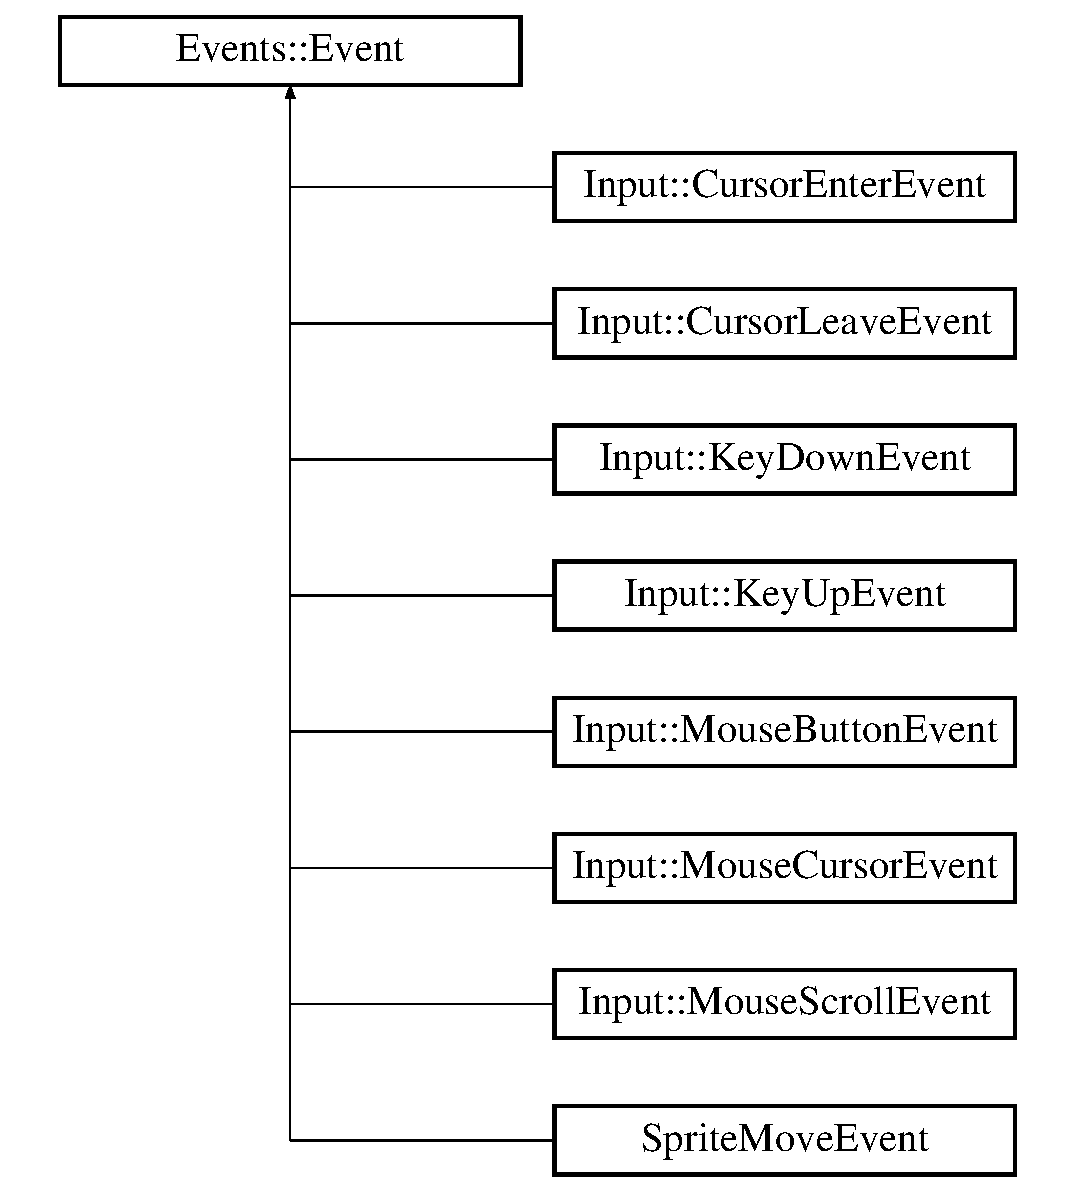
\includegraphics[height=9.000000cm]{class_events_1_1_event}
\end{center}
\end{figure}
\subsection*{Public Member Functions}
\begin{DoxyCompactItemize}
\item 
\hyperlink{class_events_1_1_event_a9252aa477066e3af6caed1d09274c712}{Event} (const \hyperlink{namespace_events_a85b018e2484fb7e336c3bb03bd41816a}{Event\+Type} \&\hyperlink{class_events_1_1_event_a91305fc66f4bda9a080e676e2971e109}{type})
\item 
const \hyperlink{namespace_events_a85b018e2484fb7e336c3bb03bd41816a}{Event\+Type} \hyperlink{class_events_1_1_event_aa88c9245f939a871f74acd0f5b3196e7}{get\+Event\+Code} () const 
\end{DoxyCompactItemize}
\subsection*{Private Attributes}
\begin{DoxyCompactItemize}
\item 
\hyperlink{namespace_events_a85b018e2484fb7e336c3bb03bd41816a}{Event\+Type} \hyperlink{class_events_1_1_event_a91305fc66f4bda9a080e676e2971e109}{type}
\end{DoxyCompactItemize}


\subsection{Constructor \& Destructor Documentation}
\hypertarget{class_events_1_1_event_a9252aa477066e3af6caed1d09274c712}{}\index{Events\+::\+Event@{Events\+::\+Event}!Event@{Event}}
\index{Event@{Event}!Events\+::\+Event@{Events\+::\+Event}}
\subsubsection[{Event}]{\setlength{\rightskip}{0pt plus 5cm}Events\+::\+Event\+::\+Event (
\begin{DoxyParamCaption}
\item[{const {\bf Event\+Type} \&}]{type}
\end{DoxyParamCaption}
)\hspace{0.3cm}{\ttfamily [inline]}}\label{class_events_1_1_event_a9252aa477066e3af6caed1d09274c712}


\subsection{Member Function Documentation}
\hypertarget{class_events_1_1_event_aa88c9245f939a871f74acd0f5b3196e7}{}\index{Events\+::\+Event@{Events\+::\+Event}!get\+Event\+Code@{get\+Event\+Code}}
\index{get\+Event\+Code@{get\+Event\+Code}!Events\+::\+Event@{Events\+::\+Event}}
\subsubsection[{get\+Event\+Code}]{\setlength{\rightskip}{0pt plus 5cm}const {\bf Event\+Type} Events\+::\+Event\+::get\+Event\+Code (
\begin{DoxyParamCaption}
{}
\end{DoxyParamCaption}
) const\hspace{0.3cm}{\ttfamily [inline]}}\label{class_events_1_1_event_aa88c9245f939a871f74acd0f5b3196e7}


\subsection{Member Data Documentation}
\hypertarget{class_events_1_1_event_a91305fc66f4bda9a080e676e2971e109}{}\index{Events\+::\+Event@{Events\+::\+Event}!type@{type}}
\index{type@{type}!Events\+::\+Event@{Events\+::\+Event}}
\subsubsection[{type}]{\setlength{\rightskip}{0pt plus 5cm}{\bf Event\+Type} Events\+::\+Event\+::type\hspace{0.3cm}{\ttfamily [private]}}\label{class_events_1_1_event_a91305fc66f4bda9a080e676e2971e109}


The documentation for this class was generated from the following file\+:\begin{DoxyCompactItemize}
\item 
src/events/\hyperlink{event_8h}{event.\+h}\end{DoxyCompactItemize}

\hypertarget{class_utility_1_1_f_p_s_counter}{}\section{Utility\+:\+:F\+P\+S\+Counter Class Reference}
\label{class_utility_1_1_f_p_s_counter}\index{Utility\+::\+F\+P\+S\+Counter@{Utility\+::\+F\+P\+S\+Counter}}


{\ttfamily \#include $<$fps\+\_\+counter.\+h$>$}

\subsection*{Public Member Functions}
\begin{DoxyCompactItemize}
\item 
\hyperlink{class_utility_1_1_f_p_s_counter_a5e76d827002c0d0e4217f43b998d6f1e}{F\+P\+S\+Counter} (const float \hyperlink{class_utility_1_1_f_p_s_counter_a148c5309c9d72773cd39d5bb791642d4}{max\+\_\+fps})
\item 
const float \hyperlink{class_utility_1_1_f_p_s_counter_a11077d4a419a31bbd254103b68e3956b}{get\+Max\+F\+P\+S} () const noexcept
\item 
const float \hyperlink{class_utility_1_1_f_p_s_counter_a79f4857494606837a23c545d0f7e5917}{get\+Current\+F\+P\+S} () const noexcept
\item 
const float \hyperlink{class_utility_1_1_f_p_s_counter_af30e85894cd28030f940973d7c38b678}{get\+Average\+F\+P\+S} () const noexcept
\item 
void \hyperlink{class_utility_1_1_f_p_s_counter_a80612f3c0a69bafdb226a2ba9f997b0d}{reset\+Average\+F\+P\+S} () noexcept
\item 
const float \hyperlink{class_utility_1_1_f_p_s_counter_aa068e564c963cbc82ebacffac9201a90}{assess\+Count\+And\+Get\+Delta} ()
\end{DoxyCompactItemize}
\subsection*{Private Member Functions}
\begin{DoxyCompactItemize}
\item 
void \hyperlink{class_utility_1_1_f_p_s_counter_ae99416b7341249e9deaf227e66d908ea}{sleep\+For} (const int milliseconds)
\end{DoxyCompactItemize}
\subsection*{Private Attributes}
\begin{DoxyCompactItemize}
\item 
float \hyperlink{class_utility_1_1_f_p_s_counter_a148c5309c9d72773cd39d5bb791642d4}{max\+\_\+fps}
\item 
float \hyperlink{class_utility_1_1_f_p_s_counter_a2acc1ab187653e4246fa2b08c773cb24}{current\+\_\+fps}
\item 
std\+::chrono\+::time\+\_\+point$<$ std\+::chrono\+::high\+\_\+resolution\+\_\+clock $>$ \hyperlink{class_utility_1_1_f_p_s_counter_ada67ad2c8564e63ee6e93251c40b257d}{last\+\_\+time}
\item 
std\+::chrono\+::time\+\_\+point$<$ std\+::chrono\+::high\+\_\+resolution\+\_\+clock $>$ \hyperlink{class_utility_1_1_f_p_s_counter_adbc8e757b4b1f8a4cd20b7cb21932b51}{current\+\_\+time}
\item 
float \hyperlink{class_utility_1_1_f_p_s_counter_a2f9c59b3d0e736480414d91cea7f7357}{delta}
\item 
float \hyperlink{class_utility_1_1_f_p_s_counter_a046815eb9021980aa4dda67ac03fcfea}{delta\+\_\+accum}
\item 
unsigned int \hyperlink{class_utility_1_1_f_p_s_counter_a9040813170d766efb0f1d82f742292cc}{frame\+\_\+count}
\item 
float \hyperlink{class_utility_1_1_f_p_s_counter_af222b6f51b284c7b735957b16e1187e3}{fps\+\_\+accum}
\end{DoxyCompactItemize}


\subsection{Constructor \& Destructor Documentation}
\hypertarget{class_utility_1_1_f_p_s_counter_a5e76d827002c0d0e4217f43b998d6f1e}{}\index{Utility\+::\+F\+P\+S\+Counter@{Utility\+::\+F\+P\+S\+Counter}!F\+P\+S\+Counter@{F\+P\+S\+Counter}}
\index{F\+P\+S\+Counter@{F\+P\+S\+Counter}!Utility\+::\+F\+P\+S\+Counter@{Utility\+::\+F\+P\+S\+Counter}}
\subsubsection[{F\+P\+S\+Counter}]{\setlength{\rightskip}{0pt plus 5cm}Utility\+::\+F\+P\+S\+Counter\+::\+F\+P\+S\+Counter (
\begin{DoxyParamCaption}
\item[{const float}]{max\+\_\+fps = {\ttfamily 0.0f}}
\end{DoxyParamCaption}
)}\label{class_utility_1_1_f_p_s_counter_a5e76d827002c0d0e4217f43b998d6f1e}


\subsection{Member Function Documentation}
\hypertarget{class_utility_1_1_f_p_s_counter_aa068e564c963cbc82ebacffac9201a90}{}\index{Utility\+::\+F\+P\+S\+Counter@{Utility\+::\+F\+P\+S\+Counter}!assess\+Count\+And\+Get\+Delta@{assess\+Count\+And\+Get\+Delta}}
\index{assess\+Count\+And\+Get\+Delta@{assess\+Count\+And\+Get\+Delta}!Utility\+::\+F\+P\+S\+Counter@{Utility\+::\+F\+P\+S\+Counter}}
\subsubsection[{assess\+Count\+And\+Get\+Delta}]{\setlength{\rightskip}{0pt plus 5cm}const float Utility\+::\+F\+P\+S\+Counter\+::assess\+Count\+And\+Get\+Delta (
\begin{DoxyParamCaption}
{}
\end{DoxyParamCaption}
)}\label{class_utility_1_1_f_p_s_counter_aa068e564c963cbc82ebacffac9201a90}
\hypertarget{class_utility_1_1_f_p_s_counter_af30e85894cd28030f940973d7c38b678}{}\index{Utility\+::\+F\+P\+S\+Counter@{Utility\+::\+F\+P\+S\+Counter}!get\+Average\+F\+P\+S@{get\+Average\+F\+P\+S}}
\index{get\+Average\+F\+P\+S@{get\+Average\+F\+P\+S}!Utility\+::\+F\+P\+S\+Counter@{Utility\+::\+F\+P\+S\+Counter}}
\subsubsection[{get\+Average\+F\+P\+S}]{\setlength{\rightskip}{0pt plus 5cm}const float Utility\+::\+F\+P\+S\+Counter\+::get\+Average\+F\+P\+S (
\begin{DoxyParamCaption}
{}
\end{DoxyParamCaption}
) const\hspace{0.3cm}{\ttfamily [noexcept]}}\label{class_utility_1_1_f_p_s_counter_af30e85894cd28030f940973d7c38b678}
\hypertarget{class_utility_1_1_f_p_s_counter_a79f4857494606837a23c545d0f7e5917}{}\index{Utility\+::\+F\+P\+S\+Counter@{Utility\+::\+F\+P\+S\+Counter}!get\+Current\+F\+P\+S@{get\+Current\+F\+P\+S}}
\index{get\+Current\+F\+P\+S@{get\+Current\+F\+P\+S}!Utility\+::\+F\+P\+S\+Counter@{Utility\+::\+F\+P\+S\+Counter}}
\subsubsection[{get\+Current\+F\+P\+S}]{\setlength{\rightskip}{0pt plus 5cm}const float Utility\+::\+F\+P\+S\+Counter\+::get\+Current\+F\+P\+S (
\begin{DoxyParamCaption}
{}
\end{DoxyParamCaption}
) const\hspace{0.3cm}{\ttfamily [noexcept]}}\label{class_utility_1_1_f_p_s_counter_a79f4857494606837a23c545d0f7e5917}
\hypertarget{class_utility_1_1_f_p_s_counter_a11077d4a419a31bbd254103b68e3956b}{}\index{Utility\+::\+F\+P\+S\+Counter@{Utility\+::\+F\+P\+S\+Counter}!get\+Max\+F\+P\+S@{get\+Max\+F\+P\+S}}
\index{get\+Max\+F\+P\+S@{get\+Max\+F\+P\+S}!Utility\+::\+F\+P\+S\+Counter@{Utility\+::\+F\+P\+S\+Counter}}
\subsubsection[{get\+Max\+F\+P\+S}]{\setlength{\rightskip}{0pt plus 5cm}const float Utility\+::\+F\+P\+S\+Counter\+::get\+Max\+F\+P\+S (
\begin{DoxyParamCaption}
{}
\end{DoxyParamCaption}
) const\hspace{0.3cm}{\ttfamily [noexcept]}}\label{class_utility_1_1_f_p_s_counter_a11077d4a419a31bbd254103b68e3956b}
\hypertarget{class_utility_1_1_f_p_s_counter_a80612f3c0a69bafdb226a2ba9f997b0d}{}\index{Utility\+::\+F\+P\+S\+Counter@{Utility\+::\+F\+P\+S\+Counter}!reset\+Average\+F\+P\+S@{reset\+Average\+F\+P\+S}}
\index{reset\+Average\+F\+P\+S@{reset\+Average\+F\+P\+S}!Utility\+::\+F\+P\+S\+Counter@{Utility\+::\+F\+P\+S\+Counter}}
\subsubsection[{reset\+Average\+F\+P\+S}]{\setlength{\rightskip}{0pt plus 5cm}void Utility\+::\+F\+P\+S\+Counter\+::reset\+Average\+F\+P\+S (
\begin{DoxyParamCaption}
{}
\end{DoxyParamCaption}
)\hspace{0.3cm}{\ttfamily [noexcept]}}\label{class_utility_1_1_f_p_s_counter_a80612f3c0a69bafdb226a2ba9f997b0d}
\hypertarget{class_utility_1_1_f_p_s_counter_ae99416b7341249e9deaf227e66d908ea}{}\index{Utility\+::\+F\+P\+S\+Counter@{Utility\+::\+F\+P\+S\+Counter}!sleep\+For@{sleep\+For}}
\index{sleep\+For@{sleep\+For}!Utility\+::\+F\+P\+S\+Counter@{Utility\+::\+F\+P\+S\+Counter}}
\subsubsection[{sleep\+For}]{\setlength{\rightskip}{0pt plus 5cm}void Utility\+::\+F\+P\+S\+Counter\+::sleep\+For (
\begin{DoxyParamCaption}
\item[{const int}]{milliseconds}
\end{DoxyParamCaption}
)\hspace{0.3cm}{\ttfamily [private]}}\label{class_utility_1_1_f_p_s_counter_ae99416b7341249e9deaf227e66d908ea}


\subsection{Member Data Documentation}
\hypertarget{class_utility_1_1_f_p_s_counter_a2acc1ab187653e4246fa2b08c773cb24}{}\index{Utility\+::\+F\+P\+S\+Counter@{Utility\+::\+F\+P\+S\+Counter}!current\+\_\+fps@{current\+\_\+fps}}
\index{current\+\_\+fps@{current\+\_\+fps}!Utility\+::\+F\+P\+S\+Counter@{Utility\+::\+F\+P\+S\+Counter}}
\subsubsection[{current\+\_\+fps}]{\setlength{\rightskip}{0pt plus 5cm}float Utility\+::\+F\+P\+S\+Counter\+::current\+\_\+fps\hspace{0.3cm}{\ttfamily [private]}}\label{class_utility_1_1_f_p_s_counter_a2acc1ab187653e4246fa2b08c773cb24}
\hypertarget{class_utility_1_1_f_p_s_counter_adbc8e757b4b1f8a4cd20b7cb21932b51}{}\index{Utility\+::\+F\+P\+S\+Counter@{Utility\+::\+F\+P\+S\+Counter}!current\+\_\+time@{current\+\_\+time}}
\index{current\+\_\+time@{current\+\_\+time}!Utility\+::\+F\+P\+S\+Counter@{Utility\+::\+F\+P\+S\+Counter}}
\subsubsection[{current\+\_\+time}]{\setlength{\rightskip}{0pt plus 5cm}std\+::chrono\+::time\+\_\+point$<$std\+::chrono\+::high\+\_\+resolution\+\_\+clock$>$ Utility\+::\+F\+P\+S\+Counter\+::current\+\_\+time\hspace{0.3cm}{\ttfamily [private]}}\label{class_utility_1_1_f_p_s_counter_adbc8e757b4b1f8a4cd20b7cb21932b51}
\hypertarget{class_utility_1_1_f_p_s_counter_a2f9c59b3d0e736480414d91cea7f7357}{}\index{Utility\+::\+F\+P\+S\+Counter@{Utility\+::\+F\+P\+S\+Counter}!delta@{delta}}
\index{delta@{delta}!Utility\+::\+F\+P\+S\+Counter@{Utility\+::\+F\+P\+S\+Counter}}
\subsubsection[{delta}]{\setlength{\rightskip}{0pt plus 5cm}float Utility\+::\+F\+P\+S\+Counter\+::delta\hspace{0.3cm}{\ttfamily [private]}}\label{class_utility_1_1_f_p_s_counter_a2f9c59b3d0e736480414d91cea7f7357}
\hypertarget{class_utility_1_1_f_p_s_counter_a046815eb9021980aa4dda67ac03fcfea}{}\index{Utility\+::\+F\+P\+S\+Counter@{Utility\+::\+F\+P\+S\+Counter}!delta\+\_\+accum@{delta\+\_\+accum}}
\index{delta\+\_\+accum@{delta\+\_\+accum}!Utility\+::\+F\+P\+S\+Counter@{Utility\+::\+F\+P\+S\+Counter}}
\subsubsection[{delta\+\_\+accum}]{\setlength{\rightskip}{0pt plus 5cm}float Utility\+::\+F\+P\+S\+Counter\+::delta\+\_\+accum\hspace{0.3cm}{\ttfamily [private]}}\label{class_utility_1_1_f_p_s_counter_a046815eb9021980aa4dda67ac03fcfea}
\hypertarget{class_utility_1_1_f_p_s_counter_af222b6f51b284c7b735957b16e1187e3}{}\index{Utility\+::\+F\+P\+S\+Counter@{Utility\+::\+F\+P\+S\+Counter}!fps\+\_\+accum@{fps\+\_\+accum}}
\index{fps\+\_\+accum@{fps\+\_\+accum}!Utility\+::\+F\+P\+S\+Counter@{Utility\+::\+F\+P\+S\+Counter}}
\subsubsection[{fps\+\_\+accum}]{\setlength{\rightskip}{0pt plus 5cm}float Utility\+::\+F\+P\+S\+Counter\+::fps\+\_\+accum\hspace{0.3cm}{\ttfamily [private]}}\label{class_utility_1_1_f_p_s_counter_af222b6f51b284c7b735957b16e1187e3}
\hypertarget{class_utility_1_1_f_p_s_counter_a9040813170d766efb0f1d82f742292cc}{}\index{Utility\+::\+F\+P\+S\+Counter@{Utility\+::\+F\+P\+S\+Counter}!frame\+\_\+count@{frame\+\_\+count}}
\index{frame\+\_\+count@{frame\+\_\+count}!Utility\+::\+F\+P\+S\+Counter@{Utility\+::\+F\+P\+S\+Counter}}
\subsubsection[{frame\+\_\+count}]{\setlength{\rightskip}{0pt plus 5cm}unsigned int Utility\+::\+F\+P\+S\+Counter\+::frame\+\_\+count\hspace{0.3cm}{\ttfamily [private]}}\label{class_utility_1_1_f_p_s_counter_a9040813170d766efb0f1d82f742292cc}
\hypertarget{class_utility_1_1_f_p_s_counter_ada67ad2c8564e63ee6e93251c40b257d}{}\index{Utility\+::\+F\+P\+S\+Counter@{Utility\+::\+F\+P\+S\+Counter}!last\+\_\+time@{last\+\_\+time}}
\index{last\+\_\+time@{last\+\_\+time}!Utility\+::\+F\+P\+S\+Counter@{Utility\+::\+F\+P\+S\+Counter}}
\subsubsection[{last\+\_\+time}]{\setlength{\rightskip}{0pt plus 5cm}std\+::chrono\+::time\+\_\+point$<$std\+::chrono\+::high\+\_\+resolution\+\_\+clock$>$ Utility\+::\+F\+P\+S\+Counter\+::last\+\_\+time\hspace{0.3cm}{\ttfamily [private]}}\label{class_utility_1_1_f_p_s_counter_ada67ad2c8564e63ee6e93251c40b257d}
\hypertarget{class_utility_1_1_f_p_s_counter_a148c5309c9d72773cd39d5bb791642d4}{}\index{Utility\+::\+F\+P\+S\+Counter@{Utility\+::\+F\+P\+S\+Counter}!max\+\_\+fps@{max\+\_\+fps}}
\index{max\+\_\+fps@{max\+\_\+fps}!Utility\+::\+F\+P\+S\+Counter@{Utility\+::\+F\+P\+S\+Counter}}
\subsubsection[{max\+\_\+fps}]{\setlength{\rightskip}{0pt plus 5cm}float Utility\+::\+F\+P\+S\+Counter\+::max\+\_\+fps\hspace{0.3cm}{\ttfamily [private]}}\label{class_utility_1_1_f_p_s_counter_a148c5309c9d72773cd39d5bb791642d4}


The documentation for this class was generated from the following files\+:\begin{DoxyCompactItemize}
\item 
src/utility/\hyperlink{fps__counter_8h}{fps\+\_\+counter.\+h}\item 
src/utility/\hyperlink{fps__counter_8cpp}{fps\+\_\+counter.\+cpp}\end{DoxyCompactItemize}

\hypertarget{class_graphics_1_1_graphics_system}{}\section{Graphics\+:\+:Graphics\+System Class Reference}
\label{class_graphics_1_1_graphics_system}\index{Graphics\+::\+Graphics\+System@{Graphics\+::\+Graphics\+System}}


{\ttfamily \#include $<$graphics\+\_\+system.\+h$>$}

\subsection*{Public Member Functions}
\begin{DoxyCompactItemize}
\item 
\hyperlink{class_graphics_1_1_graphics_system_a748459586ae5ea2aa8721dddb8660de6}{Graphics\+System} ()
\item 
\hyperlink{class_graphics_1_1_graphics_system_a6504df337bfae3a08abc8a63deb6df37}{$\sim$\+Graphics\+System} ()
\item 
void \hyperlink{class_graphics_1_1_graphics_system_a0666cab04b1c7f3ca4dac67f7529cace}{initialize} (const int width, const int height, std\+::string name, const \hyperlink{class_graphics_1_1_window_exit_functor}{Window\+Exit\+Functor} \&\hyperlink{class_graphics_1_1_graphics_system_ac31d552052e7afd10043456ee9393e1a}{window\+\_\+exit}, const double \hyperlink{class_graphics_1_1_graphics_system_ad963821cfb09e6a0e672cf6876e944dd}{max\+\_\+fps}=0.\+0)
\begin{DoxyCompactList}\small\item\em Initializes the graphics system. \end{DoxyCompactList}\item 
const bool \hyperlink{class_graphics_1_1_graphics_system_a1bd027633e66df5a65f2df33952d1dbd}{is\+Initialized} () const noexcept
\begin{DoxyCompactList}\small\item\em Getter to see if system is initialized. \end{DoxyCompactList}\item 
void \hyperlink{class_graphics_1_1_graphics_system_af222ab3a8a83796ad1c12ccf95a6f37a}{render\+Loop} ()
\item 
const int \hyperlink{class_graphics_1_1_graphics_system_a09710fc777ac4db1b44c63c2921d217f}{window\+Height} ()
\begin{DoxyCompactList}\small\item\em Getter for the window width. \end{DoxyCompactList}\item 
const int \hyperlink{class_graphics_1_1_graphics_system_adab3606d554a85ca13aaaec29ceee68c}{window\+Width} ()
\begin{DoxyCompactList}\small\item\em Getter for the window height. \end{DoxyCompactList}\item 
const std\+::string \hyperlink{class_graphics_1_1_graphics_system_a691efb4de942f8da79ecbcf626280724}{window\+Name} () const noexcept
\begin{DoxyCompactList}\small\item\em Getter for the window name. \end{DoxyCompactList}\item 
const int \hyperlink{class_graphics_1_1_graphics_system_ac35c2d3d32e1264b8daad6d59c3aba57}{add\+Renderable} (std\+::shared\+\_\+ptr$<$ \hyperlink{class_graphics_1_1_renderable}{Graphics\+::\+Renderable} $>$ renderable)
\begin{DoxyCompactList}\small\item\em Adds a renderable to the renderable pool. \end{DoxyCompactList}\item 
const bool \hyperlink{class_graphics_1_1_graphics_system_a476b0e6945c37c7b2d48bddcf246a389}{remove\+Renderable} (const int id)
\begin{DoxyCompactList}\small\item\em Removes a renderable from the renderable pool. \end{DoxyCompactList}\item 
const int \hyperlink{class_graphics_1_1_graphics_system_a2b37c3e6f53707002c72c38062be6617}{renderables\+Count} ()
\begin{DoxyCompactList}\small\item\em Returns the number of renderables currently in the system. \end{DoxyCompactList}\item 
const double \hyperlink{class_graphics_1_1_graphics_system_a3266a6af7dd48b4e0501953a5a92d9ee}{get\+Max\+F\+P\+S} () const noexcept
\begin{DoxyCompactList}\small\item\em Returns the max F\+P\+S set on the graphics system. \end{DoxyCompactList}\item 
const double \hyperlink{class_graphics_1_1_graphics_system_a155246106fb6bf556caab7ff9e826524}{get\+Current\+F\+P\+S} () const noexcept
\begin{DoxyCompactList}\small\item\em Returns the current running F\+P\+S on the graphics system. \end{DoxyCompactList}\item 
G\+L\+F\+Wwindow $\ast$ \hyperlink{class_graphics_1_1_graphics_system_a0692ae8d8615f820ed36615e9619fe68}{get\+Current\+Window} () noexcept
\item 
void \hyperlink{class_graphics_1_1_graphics_system_a629d2fe80f761f4f4004ba74ad458e3f}{destroy} ()
\begin{DoxyCompactList}\small\item\em Closes window, and destroys G\+L\+F\+W context. \end{DoxyCompactList}\end{DoxyCompactItemize}
\subsection*{Static Private Member Functions}
\begin{DoxyCompactItemize}
\item 
static void \hyperlink{class_graphics_1_1_graphics_system_a0e3ea1d3785e868d7a1318b4c9c15878}{error\+Callback} (int error, const char $\ast$description)
\end{DoxyCompactItemize}
\subsection*{Private Attributes}
\begin{DoxyCompactItemize}
\item 
G\+L\+F\+Wwindow $\ast$ \hyperlink{class_graphics_1_1_graphics_system_a4430d61bb3fd528b617e8fea26744a8c}{window}
\item 
bool \hyperlink{class_graphics_1_1_graphics_system_a7228e859a8b7da7d9cbc3e151ab2df72}{initialized}
\item 
std\+::string \hyperlink{class_graphics_1_1_graphics_system_a7b543ac0f4323ec286519a3dfef0df1c}{window\+\_\+title}
\item 
std\+::map$<$ int, std\+::shared\+\_\+ptr$<$ \hyperlink{class_graphics_1_1_renderable}{Graphics\+::\+Renderable} $>$ $>$ \hyperlink{class_graphics_1_1_graphics_system_a5dab770243e04860495f894184ef63bb}{renderables\+\_\+map}
\item 
std\+::mutex \hyperlink{class_graphics_1_1_graphics_system_a2e9549405884607a5922a7023a1d2b38}{renderables\+\_\+mutex}
\item 
int \hyperlink{class_graphics_1_1_graphics_system_a950f878ddd2ca0b13a715f4300447903}{next\+\_\+id}
\item 
double \hyperlink{class_graphics_1_1_graphics_system_ad963821cfb09e6a0e672cf6876e944dd}{max\+\_\+fps}
\item 
std\+::atomic$<$ double $>$ \hyperlink{class_graphics_1_1_graphics_system_aa46f6a4cdcae7ff4603c11a650b2986d}{current\+\_\+fps}
\item 
\hyperlink{class_graphics_1_1_window_exit_functor}{Window\+Exit\+Functor} \hyperlink{class_graphics_1_1_graphics_system_ac31d552052e7afd10043456ee9393e1a}{window\+\_\+exit}
\end{DoxyCompactItemize}


\subsection{Constructor \& Destructor Documentation}
\hypertarget{class_graphics_1_1_graphics_system_a748459586ae5ea2aa8721dddb8660de6}{}\index{Graphics\+::\+Graphics\+System@{Graphics\+::\+Graphics\+System}!Graphics\+System@{Graphics\+System}}
\index{Graphics\+System@{Graphics\+System}!Graphics\+::\+Graphics\+System@{Graphics\+::\+Graphics\+System}}
\subsubsection[{Graphics\+System}]{\setlength{\rightskip}{0pt plus 5cm}Graphics\+::\+Graphics\+System\+::\+Graphics\+System (
\begin{DoxyParamCaption}
{}
\end{DoxyParamCaption}
)}\label{class_graphics_1_1_graphics_system_a748459586ae5ea2aa8721dddb8660de6}
\hypertarget{class_graphics_1_1_graphics_system_a6504df337bfae3a08abc8a63deb6df37}{}\index{Graphics\+::\+Graphics\+System@{Graphics\+::\+Graphics\+System}!````~Graphics\+System@{$\sim$\+Graphics\+System}}
\index{````~Graphics\+System@{$\sim$\+Graphics\+System}!Graphics\+::\+Graphics\+System@{Graphics\+::\+Graphics\+System}}
\subsubsection[{$\sim$\+Graphics\+System}]{\setlength{\rightskip}{0pt plus 5cm}Graphics\+::\+Graphics\+System\+::$\sim$\+Graphics\+System (
\begin{DoxyParamCaption}
{}
\end{DoxyParamCaption}
)}\label{class_graphics_1_1_graphics_system_a6504df337bfae3a08abc8a63deb6df37}


\subsection{Member Function Documentation}
\hypertarget{class_graphics_1_1_graphics_system_ac35c2d3d32e1264b8daad6d59c3aba57}{}\index{Graphics\+::\+Graphics\+System@{Graphics\+::\+Graphics\+System}!add\+Renderable@{add\+Renderable}}
\index{add\+Renderable@{add\+Renderable}!Graphics\+::\+Graphics\+System@{Graphics\+::\+Graphics\+System}}
\subsubsection[{add\+Renderable}]{\setlength{\rightskip}{0pt plus 5cm}const int Graphics\+::\+Graphics\+System\+::add\+Renderable (
\begin{DoxyParamCaption}
\item[{std\+::shared\+\_\+ptr$<$ {\bf Graphics\+::\+Renderable} $>$}]{renderable}
\end{DoxyParamCaption}
)}\label{class_graphics_1_1_graphics_system_ac35c2d3d32e1264b8daad6d59c3aba57}


Adds a renderable to the renderable pool. 

Added to the pool of renderables that can be rendered during the update loop.


\begin{DoxyParams}{Parameters}
{\em renderable} & Shared Pointer to a previously created renderable \\
\hline
\end{DoxyParams}
\begin{DoxyReturn}{Returns}
id integer of the renderable 
\end{DoxyReturn}
\hypertarget{class_graphics_1_1_graphics_system_a629d2fe80f761f4f4004ba74ad458e3f}{}\index{Graphics\+::\+Graphics\+System@{Graphics\+::\+Graphics\+System}!destroy@{destroy}}
\index{destroy@{destroy}!Graphics\+::\+Graphics\+System@{Graphics\+::\+Graphics\+System}}
\subsubsection[{destroy}]{\setlength{\rightskip}{0pt plus 5cm}void Graphics\+::\+Graphics\+System\+::destroy (
\begin{DoxyParamCaption}
{}
\end{DoxyParamCaption}
)}\label{class_graphics_1_1_graphics_system_a629d2fe80f761f4f4004ba74ad458e3f}


Closes window, and destroys G\+L\+F\+W context. 

This closes the window created by G\+L\+F\+W and terminates glfw. Initialize must be called to get another window. \hypertarget{class_graphics_1_1_graphics_system_a0e3ea1d3785e868d7a1318b4c9c15878}{}\index{Graphics\+::\+Graphics\+System@{Graphics\+::\+Graphics\+System}!error\+Callback@{error\+Callback}}
\index{error\+Callback@{error\+Callback}!Graphics\+::\+Graphics\+System@{Graphics\+::\+Graphics\+System}}
\subsubsection[{error\+Callback}]{\setlength{\rightskip}{0pt plus 5cm}void Graphics\+::\+Graphics\+System\+::error\+Callback (
\begin{DoxyParamCaption}
\item[{int}]{error, }
\item[{const char $\ast$}]{description}
\end{DoxyParamCaption}
)\hspace{0.3cm}{\ttfamily [static]}, {\ttfamily [private]}}\label{class_graphics_1_1_graphics_system_a0e3ea1d3785e868d7a1318b4c9c15878}
\hypertarget{class_graphics_1_1_graphics_system_a155246106fb6bf556caab7ff9e826524}{}\index{Graphics\+::\+Graphics\+System@{Graphics\+::\+Graphics\+System}!get\+Current\+F\+P\+S@{get\+Current\+F\+P\+S}}
\index{get\+Current\+F\+P\+S@{get\+Current\+F\+P\+S}!Graphics\+::\+Graphics\+System@{Graphics\+::\+Graphics\+System}}
\subsubsection[{get\+Current\+F\+P\+S}]{\setlength{\rightskip}{0pt plus 5cm}const double Graphics\+::\+Graphics\+System\+::get\+Current\+F\+P\+S (
\begin{DoxyParamCaption}
{}
\end{DoxyParamCaption}
) const\hspace{0.3cm}{\ttfamily [noexcept]}}\label{class_graphics_1_1_graphics_system_a155246106fb6bf556caab7ff9e826524}


Returns the current running F\+P\+S on the graphics system. 

This is the current fps that has been recorded as the graphics system is running. \begin{DoxyReturn}{Returns}
double containing the current fps 
\end{DoxyReturn}
\hypertarget{class_graphics_1_1_graphics_system_a0692ae8d8615f820ed36615e9619fe68}{}\index{Graphics\+::\+Graphics\+System@{Graphics\+::\+Graphics\+System}!get\+Current\+Window@{get\+Current\+Window}}
\index{get\+Current\+Window@{get\+Current\+Window}!Graphics\+::\+Graphics\+System@{Graphics\+::\+Graphics\+System}}
\subsubsection[{get\+Current\+Window}]{\setlength{\rightskip}{0pt plus 5cm}G\+L\+F\+Wwindow $\ast$ Graphics\+::\+Graphics\+System\+::get\+Current\+Window (
\begin{DoxyParamCaption}
{}
\end{DoxyParamCaption}
)\hspace{0.3cm}{\ttfamily [noexcept]}}\label{class_graphics_1_1_graphics_system_a0692ae8d8615f820ed36615e9619fe68}
\hypertarget{class_graphics_1_1_graphics_system_a3266a6af7dd48b4e0501953a5a92d9ee}{}\index{Graphics\+::\+Graphics\+System@{Graphics\+::\+Graphics\+System}!get\+Max\+F\+P\+S@{get\+Max\+F\+P\+S}}
\index{get\+Max\+F\+P\+S@{get\+Max\+F\+P\+S}!Graphics\+::\+Graphics\+System@{Graphics\+::\+Graphics\+System}}
\subsubsection[{get\+Max\+F\+P\+S}]{\setlength{\rightskip}{0pt plus 5cm}const double Graphics\+::\+Graphics\+System\+::get\+Max\+F\+P\+S (
\begin{DoxyParamCaption}
{}
\end{DoxyParamCaption}
) const\hspace{0.3cm}{\ttfamily [noexcept]}}\label{class_graphics_1_1_graphics_system_a3266a6af7dd48b4e0501953a5a92d9ee}


Returns the max F\+P\+S set on the graphics system. 

This is the highest frames per second the graphics system can run at (to allow things like vsync) \begin{DoxyReturn}{Returns}
double containing the max fps 
\end{DoxyReturn}
\hypertarget{class_graphics_1_1_graphics_system_a0666cab04b1c7f3ca4dac67f7529cace}{}\index{Graphics\+::\+Graphics\+System@{Graphics\+::\+Graphics\+System}!initialize@{initialize}}
\index{initialize@{initialize}!Graphics\+::\+Graphics\+System@{Graphics\+::\+Graphics\+System}}
\subsubsection[{initialize}]{\setlength{\rightskip}{0pt plus 5cm}void Graphics\+::\+Graphics\+System\+::initialize (
\begin{DoxyParamCaption}
\item[{const int}]{width, }
\item[{const int}]{height, }
\item[{std\+::string}]{name, }
\item[{const {\bf Window\+Exit\+Functor} \&}]{window\+\_\+exit, }
\item[{const double}]{max\+\_\+fps = {\ttfamily 0.0}}
\end{DoxyParamCaption}
)}\label{class_graphics_1_1_graphics_system_a0666cab04b1c7f3ca4dac67f7529cace}


Initializes the graphics system. 

This function initializes the graphics system by creating a G\+L\+F\+W based window at the specified size, and having the supplied name as the window title. Max F\+P\+S can also be supplied to allow V\+S\+Y\+N\+C.


\begin{DoxyParams}{Parameters}
{\em width} & window width in px \\
\hline
{\em height} & window height in px \\
\hline
{\em name} & string containing the name of the window to be built \\
\hline
{\em max\+\_\+fps} & double containing the max allowed fps. Default 0.\+0. \\
\hline
\end{DoxyParams}
\hypertarget{class_graphics_1_1_graphics_system_a1bd027633e66df5a65f2df33952d1dbd}{}\index{Graphics\+::\+Graphics\+System@{Graphics\+::\+Graphics\+System}!is\+Initialized@{is\+Initialized}}
\index{is\+Initialized@{is\+Initialized}!Graphics\+::\+Graphics\+System@{Graphics\+::\+Graphics\+System}}
\subsubsection[{is\+Initialized}]{\setlength{\rightskip}{0pt plus 5cm}const bool Graphics\+::\+Graphics\+System\+::is\+Initialized (
\begin{DoxyParamCaption}
{}
\end{DoxyParamCaption}
) const\hspace{0.3cm}{\ttfamily [noexcept]}}\label{class_graphics_1_1_graphics_system_a1bd027633e66df5a65f2df33952d1dbd}


Getter to see if system is initialized. 

Will return true after \hyperlink{class_graphics_1_1_graphics_system_a0666cab04b1c7f3ca4dac67f7529cace}{initialize()} is called. \begin{DoxyReturn}{Returns}
true if \hyperlink{class_graphics_1_1_graphics_system_a7228e859a8b7da7d9cbc3e151ab2df72}{initialized()} has been called, false otherwise 
\end{DoxyReturn}
\hypertarget{class_graphics_1_1_graphics_system_a476b0e6945c37c7b2d48bddcf246a389}{}\index{Graphics\+::\+Graphics\+System@{Graphics\+::\+Graphics\+System}!remove\+Renderable@{remove\+Renderable}}
\index{remove\+Renderable@{remove\+Renderable}!Graphics\+::\+Graphics\+System@{Graphics\+::\+Graphics\+System}}
\subsubsection[{remove\+Renderable}]{\setlength{\rightskip}{0pt plus 5cm}const bool Graphics\+::\+Graphics\+System\+::remove\+Renderable (
\begin{DoxyParamCaption}
\item[{const int}]{id}
\end{DoxyParamCaption}
)}\label{class_graphics_1_1_graphics_system_a476b0e6945c37c7b2d48bddcf246a389}


Removes a renderable from the renderable pool. 

Removed from the pool of renderables to take it out of the update loop.


\begin{DoxyParams}{Parameters}
{\em id} & id integer of renderable to remove \\
\hline
\end{DoxyParams}
\begin{DoxyReturn}{Returns}
true if successful, false if it didn\textquotesingle{}t exist 
\end{DoxyReturn}
\hypertarget{class_graphics_1_1_graphics_system_a2b37c3e6f53707002c72c38062be6617}{}\index{Graphics\+::\+Graphics\+System@{Graphics\+::\+Graphics\+System}!renderables\+Count@{renderables\+Count}}
\index{renderables\+Count@{renderables\+Count}!Graphics\+::\+Graphics\+System@{Graphics\+::\+Graphics\+System}}
\subsubsection[{renderables\+Count}]{\setlength{\rightskip}{0pt plus 5cm}const int Graphics\+::\+Graphics\+System\+::renderables\+Count (
\begin{DoxyParamCaption}
{}
\end{DoxyParamCaption}
)}\label{class_graphics_1_1_graphics_system_a2b37c3e6f53707002c72c38062be6617}


Returns the number of renderables currently in the system. 

This returns the number of renderables that have been added to the system, and are ready to be updated and rendered. \begin{DoxyReturn}{Returns}
integer representing number of renderables in the system 
\end{DoxyReturn}
\hypertarget{class_graphics_1_1_graphics_system_af222ab3a8a83796ad1c12ccf95a6f37a}{}\index{Graphics\+::\+Graphics\+System@{Graphics\+::\+Graphics\+System}!render\+Loop@{render\+Loop}}
\index{render\+Loop@{render\+Loop}!Graphics\+::\+Graphics\+System@{Graphics\+::\+Graphics\+System}}
\subsubsection[{render\+Loop}]{\setlength{\rightskip}{0pt plus 5cm}void Graphics\+::\+Graphics\+System\+::render\+Loop (
\begin{DoxyParamCaption}
{}
\end{DoxyParamCaption}
)}\label{class_graphics_1_1_graphics_system_af222ab3a8a83796ad1c12ccf95a6f37a}
\hypertarget{class_graphics_1_1_graphics_system_a09710fc777ac4db1b44c63c2921d217f}{}\index{Graphics\+::\+Graphics\+System@{Graphics\+::\+Graphics\+System}!window\+Height@{window\+Height}}
\index{window\+Height@{window\+Height}!Graphics\+::\+Graphics\+System@{Graphics\+::\+Graphics\+System}}
\subsubsection[{window\+Height}]{\setlength{\rightskip}{0pt plus 5cm}const int Graphics\+::\+Graphics\+System\+::window\+Height (
\begin{DoxyParamCaption}
{}
\end{DoxyParamCaption}
)}\label{class_graphics_1_1_graphics_system_a09710fc777ac4db1b44c63c2921d217f}


Getter for the window width. 

This Pings G\+L\+F\+W to get the width of the window. \begin{DoxyReturn}{Returns}
integer denoting pixel width of window 
\end{DoxyReturn}
\hypertarget{class_graphics_1_1_graphics_system_a691efb4de942f8da79ecbcf626280724}{}\index{Graphics\+::\+Graphics\+System@{Graphics\+::\+Graphics\+System}!window\+Name@{window\+Name}}
\index{window\+Name@{window\+Name}!Graphics\+::\+Graphics\+System@{Graphics\+::\+Graphics\+System}}
\subsubsection[{window\+Name}]{\setlength{\rightskip}{0pt plus 5cm}const std\+::string Graphics\+::\+Graphics\+System\+::window\+Name (
\begin{DoxyParamCaption}
{}
\end{DoxyParamCaption}
) const\hspace{0.3cm}{\ttfamily [noexcept]}}\label{class_graphics_1_1_graphics_system_a691efb4de942f8da79ecbcf626280724}


Getter for the window name. 

This will return the name of the window \begin{DoxyReturn}{Returns}
a string that is the name of the window 
\end{DoxyReturn}
\hypertarget{class_graphics_1_1_graphics_system_adab3606d554a85ca13aaaec29ceee68c}{}\index{Graphics\+::\+Graphics\+System@{Graphics\+::\+Graphics\+System}!window\+Width@{window\+Width}}
\index{window\+Width@{window\+Width}!Graphics\+::\+Graphics\+System@{Graphics\+::\+Graphics\+System}}
\subsubsection[{window\+Width}]{\setlength{\rightskip}{0pt plus 5cm}const int Graphics\+::\+Graphics\+System\+::window\+Width (
\begin{DoxyParamCaption}
{}
\end{DoxyParamCaption}
)}\label{class_graphics_1_1_graphics_system_adab3606d554a85ca13aaaec29ceee68c}


Getter for the window height. 

This Pings G\+L\+F\+W to get the height of the window. \begin{DoxyReturn}{Returns}
integer denoting pixel height of window 
\end{DoxyReturn}


\subsection{Member Data Documentation}
\hypertarget{class_graphics_1_1_graphics_system_aa46f6a4cdcae7ff4603c11a650b2986d}{}\index{Graphics\+::\+Graphics\+System@{Graphics\+::\+Graphics\+System}!current\+\_\+fps@{current\+\_\+fps}}
\index{current\+\_\+fps@{current\+\_\+fps}!Graphics\+::\+Graphics\+System@{Graphics\+::\+Graphics\+System}}
\subsubsection[{current\+\_\+fps}]{\setlength{\rightskip}{0pt plus 5cm}std\+::atomic$<$double$>$ Graphics\+::\+Graphics\+System\+::current\+\_\+fps\hspace{0.3cm}{\ttfamily [private]}}\label{class_graphics_1_1_graphics_system_aa46f6a4cdcae7ff4603c11a650b2986d}
\hypertarget{class_graphics_1_1_graphics_system_a7228e859a8b7da7d9cbc3e151ab2df72}{}\index{Graphics\+::\+Graphics\+System@{Graphics\+::\+Graphics\+System}!initialized@{initialized}}
\index{initialized@{initialized}!Graphics\+::\+Graphics\+System@{Graphics\+::\+Graphics\+System}}
\subsubsection[{initialized}]{\setlength{\rightskip}{0pt plus 5cm}bool Graphics\+::\+Graphics\+System\+::initialized\hspace{0.3cm}{\ttfamily [private]}}\label{class_graphics_1_1_graphics_system_a7228e859a8b7da7d9cbc3e151ab2df72}
\hypertarget{class_graphics_1_1_graphics_system_ad963821cfb09e6a0e672cf6876e944dd}{}\index{Graphics\+::\+Graphics\+System@{Graphics\+::\+Graphics\+System}!max\+\_\+fps@{max\+\_\+fps}}
\index{max\+\_\+fps@{max\+\_\+fps}!Graphics\+::\+Graphics\+System@{Graphics\+::\+Graphics\+System}}
\subsubsection[{max\+\_\+fps}]{\setlength{\rightskip}{0pt plus 5cm}double Graphics\+::\+Graphics\+System\+::max\+\_\+fps\hspace{0.3cm}{\ttfamily [private]}}\label{class_graphics_1_1_graphics_system_ad963821cfb09e6a0e672cf6876e944dd}
\hypertarget{class_graphics_1_1_graphics_system_a950f878ddd2ca0b13a715f4300447903}{}\index{Graphics\+::\+Graphics\+System@{Graphics\+::\+Graphics\+System}!next\+\_\+id@{next\+\_\+id}}
\index{next\+\_\+id@{next\+\_\+id}!Graphics\+::\+Graphics\+System@{Graphics\+::\+Graphics\+System}}
\subsubsection[{next\+\_\+id}]{\setlength{\rightskip}{0pt plus 5cm}int Graphics\+::\+Graphics\+System\+::next\+\_\+id\hspace{0.3cm}{\ttfamily [private]}}\label{class_graphics_1_1_graphics_system_a950f878ddd2ca0b13a715f4300447903}
\hypertarget{class_graphics_1_1_graphics_system_a5dab770243e04860495f894184ef63bb}{}\index{Graphics\+::\+Graphics\+System@{Graphics\+::\+Graphics\+System}!renderables\+\_\+map@{renderables\+\_\+map}}
\index{renderables\+\_\+map@{renderables\+\_\+map}!Graphics\+::\+Graphics\+System@{Graphics\+::\+Graphics\+System}}
\subsubsection[{renderables\+\_\+map}]{\setlength{\rightskip}{0pt plus 5cm}std\+::map$<$int, std\+::shared\+\_\+ptr$<${\bf Graphics\+::\+Renderable}$>$ $>$ Graphics\+::\+Graphics\+System\+::renderables\+\_\+map\hspace{0.3cm}{\ttfamily [private]}}\label{class_graphics_1_1_graphics_system_a5dab770243e04860495f894184ef63bb}
\hypertarget{class_graphics_1_1_graphics_system_a2e9549405884607a5922a7023a1d2b38}{}\index{Graphics\+::\+Graphics\+System@{Graphics\+::\+Graphics\+System}!renderables\+\_\+mutex@{renderables\+\_\+mutex}}
\index{renderables\+\_\+mutex@{renderables\+\_\+mutex}!Graphics\+::\+Graphics\+System@{Graphics\+::\+Graphics\+System}}
\subsubsection[{renderables\+\_\+mutex}]{\setlength{\rightskip}{0pt plus 5cm}std\+::mutex Graphics\+::\+Graphics\+System\+::renderables\+\_\+mutex\hspace{0.3cm}{\ttfamily [private]}}\label{class_graphics_1_1_graphics_system_a2e9549405884607a5922a7023a1d2b38}
\hypertarget{class_graphics_1_1_graphics_system_a4430d61bb3fd528b617e8fea26744a8c}{}\index{Graphics\+::\+Graphics\+System@{Graphics\+::\+Graphics\+System}!window@{window}}
\index{window@{window}!Graphics\+::\+Graphics\+System@{Graphics\+::\+Graphics\+System}}
\subsubsection[{window}]{\setlength{\rightskip}{0pt plus 5cm}G\+L\+F\+Wwindow$\ast$ Graphics\+::\+Graphics\+System\+::window\hspace{0.3cm}{\ttfamily [private]}}\label{class_graphics_1_1_graphics_system_a4430d61bb3fd528b617e8fea26744a8c}
\hypertarget{class_graphics_1_1_graphics_system_ac31d552052e7afd10043456ee9393e1a}{}\index{Graphics\+::\+Graphics\+System@{Graphics\+::\+Graphics\+System}!window\+\_\+exit@{window\+\_\+exit}}
\index{window\+\_\+exit@{window\+\_\+exit}!Graphics\+::\+Graphics\+System@{Graphics\+::\+Graphics\+System}}
\subsubsection[{window\+\_\+exit}]{\setlength{\rightskip}{0pt plus 5cm}{\bf Window\+Exit\+Functor} Graphics\+::\+Graphics\+System\+::window\+\_\+exit\hspace{0.3cm}{\ttfamily [private]}}\label{class_graphics_1_1_graphics_system_ac31d552052e7afd10043456ee9393e1a}
\hypertarget{class_graphics_1_1_graphics_system_a7b543ac0f4323ec286519a3dfef0df1c}{}\index{Graphics\+::\+Graphics\+System@{Graphics\+::\+Graphics\+System}!window\+\_\+title@{window\+\_\+title}}
\index{window\+\_\+title@{window\+\_\+title}!Graphics\+::\+Graphics\+System@{Graphics\+::\+Graphics\+System}}
\subsubsection[{window\+\_\+title}]{\setlength{\rightskip}{0pt plus 5cm}std\+::string Graphics\+::\+Graphics\+System\+::window\+\_\+title\hspace{0.3cm}{\ttfamily [private]}}\label{class_graphics_1_1_graphics_system_a7b543ac0f4323ec286519a3dfef0df1c}


The documentation for this class was generated from the following files\+:\begin{DoxyCompactItemize}
\item 
src/graphics/\hyperlink{graphics__system_8h}{graphics\+\_\+system.\+h}\item 
src/graphics/\hyperlink{graphics__system_8cpp}{graphics\+\_\+system.\+cpp}\end{DoxyCompactItemize}

\hypertarget{class_input_1_1_input_system}{}\section{Input\+:\+:Input\+System Class Reference}
\label{class_input_1_1_input_system}\index{Input\+::\+Input\+System@{Input\+::\+Input\+System}}


{\ttfamily \#include $<$input\+\_\+system.\+h$>$}

Inheritance diagram for Input\+:\+:Input\+System\+:\begin{figure}[H]
\begin{center}
\leavevmode
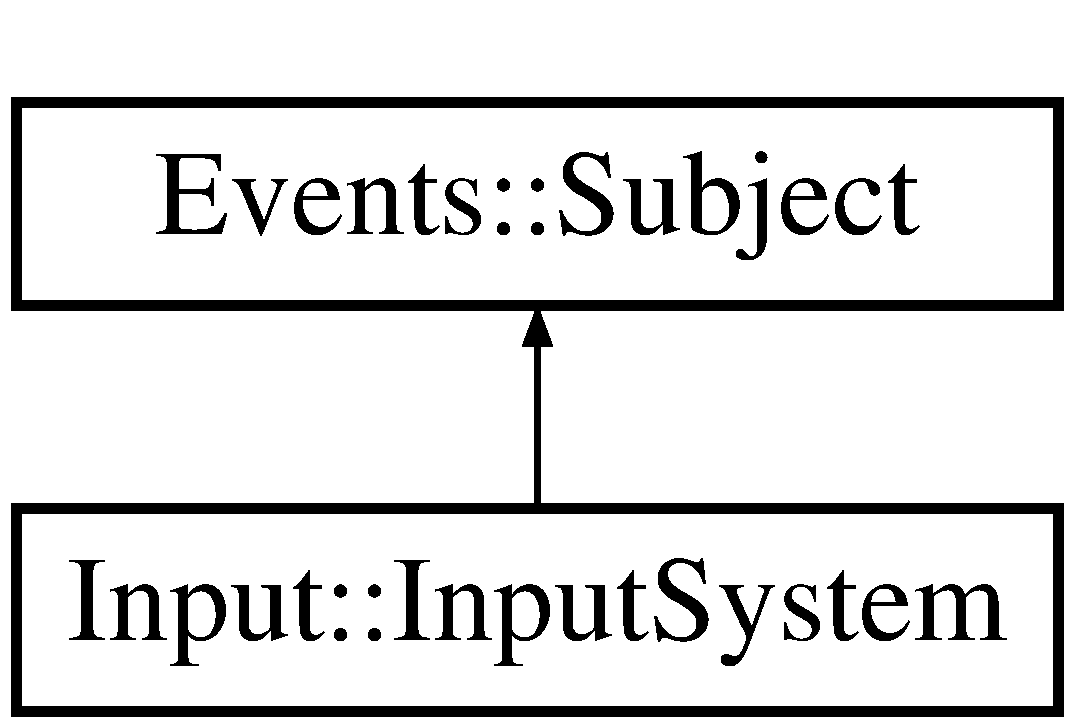
\includegraphics[height=2.000000cm]{class_input_1_1_input_system}
\end{center}
\end{figure}
\subsection*{Public Member Functions}
\begin{DoxyCompactItemize}
\item 
\hyperlink{class_input_1_1_input_system_aa754c4c6a976f808004a93dbcfcdb39e}{Input\+System} (G\+L\+F\+Wwindow $\ast$window)
\item 
void \hyperlink{class_input_1_1_input_system_a922d74d9c7b1d58785d58eb8187b90db}{poll\+For\+Input} ()
\end{DoxyCompactItemize}
\subsection*{Static Private Member Functions}
\begin{DoxyCompactItemize}
\item 
static void \hyperlink{class_input_1_1_input_system_a2a53f93797b351082ba88e65a76a59d3}{key\+Callback} (G\+L\+F\+Wwindow $\ast$window, int key, int scan\+\_\+code, int action, int mods)
\item 
static void \hyperlink{class_input_1_1_input_system_a25e317033e1c9932fca9a0f18bafba3e}{cursor\+Position\+Callback} (G\+L\+F\+Wwindow $\ast$window, double x\+\_\+pos, double y\+\_\+pos)
\item 
static void \hyperlink{class_input_1_1_input_system_a418ad9c5aeea37d4700ce108a525168c}{cursor\+Enter\+Callback} (G\+L\+F\+Wwindow $\ast$window, int entered)
\item 
static void \hyperlink{class_input_1_1_input_system_a2d52be441c72bf70dc369c1c075e252d}{mouse\+Button\+Callback} (G\+L\+F\+Wwindow $\ast$window, int button, int action, int mods)
\item 
static void \hyperlink{class_input_1_1_input_system_adcc2296baf82656e5ffbe9aa939163eb}{mouse\+Scroll\+Callback} (G\+L\+F\+Wwindow $\ast$window, double x\+\_\+offset, double y\+\_\+offset)
\end{DoxyCompactItemize}
\subsection*{Private Attributes}
\begin{DoxyCompactItemize}
\item 
std\+::map$<$ int, int $>$ \hyperlink{class_input_1_1_input_system_a7975b0aa6e26934e4676adc7eddb7afe}{last\+\_\+keys\+\_\+to\+\_\+actions}
\item 
std\+::map$<$ int, int $>$ \hyperlink{class_input_1_1_input_system_a114e8f05ef3fa1dfb9bc7846110a17df}{last\+\_\+mouse\+\_\+buttons\+\_\+to\+\_\+actions}
\end{DoxyCompactItemize}
\subsection*{Static Private Attributes}
\begin{DoxyCompactItemize}
\item 
static std\+::map$<$ int, int $>$ \hyperlink{class_input_1_1_input_system_a95d4a156b1576e4a79290d3d3f404515}{keys\+\_\+to\+\_\+actions} \{\}
\item 
static std\+::map$<$ int, int $>$ \hyperlink{class_input_1_1_input_system_aef7be617b0a51e5fbd854100212438c8}{mouse\+\_\+buttons\+\_\+to\+\_\+actions} \{\}
\item 
static glm\+::dvec2 \hyperlink{class_input_1_1_input_system_acc7d0415600059d9cc427a7734b59190}{cursor\+\_\+position} = glm\+::dvec2(0.\+0, 0.\+0)
\item 
static glm\+::dvec2 \hyperlink{class_input_1_1_input_system_a7d9b7ce763b48a16d3feff0c93a14428}{scroll\+\_\+offset} = glm\+::dvec2(0.\+0, 0.\+0)
\item 
static bool \hyperlink{class_input_1_1_input_system_a35b0b0ab2ba2e21c1b0f177a6c78a130}{cursor\+\_\+entered} = false
\item 
static bool \hyperlink{class_input_1_1_input_system_a4206748c9f2535838f63e393f9859739}{cursor\+\_\+left} = false
\end{DoxyCompactItemize}
\subsection*{Additional Inherited Members}


\subsection{Constructor \& Destructor Documentation}
\hypertarget{class_input_1_1_input_system_aa754c4c6a976f808004a93dbcfcdb39e}{}\index{Input\+::\+Input\+System@{Input\+::\+Input\+System}!Input\+System@{Input\+System}}
\index{Input\+System@{Input\+System}!Input\+::\+Input\+System@{Input\+::\+Input\+System}}
\subsubsection[{Input\+System}]{\setlength{\rightskip}{0pt plus 5cm}Input\+::\+Input\+System\+::\+Input\+System (
\begin{DoxyParamCaption}
\item[{G\+L\+F\+Wwindow $\ast$}]{window}
\end{DoxyParamCaption}
)}\label{class_input_1_1_input_system_aa754c4c6a976f808004a93dbcfcdb39e}


\subsection{Member Function Documentation}
\hypertarget{class_input_1_1_input_system_a418ad9c5aeea37d4700ce108a525168c}{}\index{Input\+::\+Input\+System@{Input\+::\+Input\+System}!cursor\+Enter\+Callback@{cursor\+Enter\+Callback}}
\index{cursor\+Enter\+Callback@{cursor\+Enter\+Callback}!Input\+::\+Input\+System@{Input\+::\+Input\+System}}
\subsubsection[{cursor\+Enter\+Callback}]{\setlength{\rightskip}{0pt plus 5cm}void Input\+::\+Input\+System\+::cursor\+Enter\+Callback (
\begin{DoxyParamCaption}
\item[{G\+L\+F\+Wwindow $\ast$}]{window, }
\item[{int}]{entered}
\end{DoxyParamCaption}
)\hspace{0.3cm}{\ttfamily [static]}, {\ttfamily [private]}}\label{class_input_1_1_input_system_a418ad9c5aeea37d4700ce108a525168c}
\hypertarget{class_input_1_1_input_system_a25e317033e1c9932fca9a0f18bafba3e}{}\index{Input\+::\+Input\+System@{Input\+::\+Input\+System}!cursor\+Position\+Callback@{cursor\+Position\+Callback}}
\index{cursor\+Position\+Callback@{cursor\+Position\+Callback}!Input\+::\+Input\+System@{Input\+::\+Input\+System}}
\subsubsection[{cursor\+Position\+Callback}]{\setlength{\rightskip}{0pt plus 5cm}void Input\+::\+Input\+System\+::cursor\+Position\+Callback (
\begin{DoxyParamCaption}
\item[{G\+L\+F\+Wwindow $\ast$}]{window, }
\item[{double}]{x\+\_\+pos, }
\item[{double}]{y\+\_\+pos}
\end{DoxyParamCaption}
)\hspace{0.3cm}{\ttfamily [static]}, {\ttfamily [private]}}\label{class_input_1_1_input_system_a25e317033e1c9932fca9a0f18bafba3e}
\hypertarget{class_input_1_1_input_system_a2a53f93797b351082ba88e65a76a59d3}{}\index{Input\+::\+Input\+System@{Input\+::\+Input\+System}!key\+Callback@{key\+Callback}}
\index{key\+Callback@{key\+Callback}!Input\+::\+Input\+System@{Input\+::\+Input\+System}}
\subsubsection[{key\+Callback}]{\setlength{\rightskip}{0pt plus 5cm}void Input\+::\+Input\+System\+::key\+Callback (
\begin{DoxyParamCaption}
\item[{G\+L\+F\+Wwindow $\ast$}]{window, }
\item[{int}]{key, }
\item[{int}]{scan\+\_\+code, }
\item[{int}]{action, }
\item[{int}]{mods}
\end{DoxyParamCaption}
)\hspace{0.3cm}{\ttfamily [static]}, {\ttfamily [private]}}\label{class_input_1_1_input_system_a2a53f93797b351082ba88e65a76a59d3}
\hypertarget{class_input_1_1_input_system_a2d52be441c72bf70dc369c1c075e252d}{}\index{Input\+::\+Input\+System@{Input\+::\+Input\+System}!mouse\+Button\+Callback@{mouse\+Button\+Callback}}
\index{mouse\+Button\+Callback@{mouse\+Button\+Callback}!Input\+::\+Input\+System@{Input\+::\+Input\+System}}
\subsubsection[{mouse\+Button\+Callback}]{\setlength{\rightskip}{0pt plus 5cm}void Input\+::\+Input\+System\+::mouse\+Button\+Callback (
\begin{DoxyParamCaption}
\item[{G\+L\+F\+Wwindow $\ast$}]{window, }
\item[{int}]{button, }
\item[{int}]{action, }
\item[{int}]{mods}
\end{DoxyParamCaption}
)\hspace{0.3cm}{\ttfamily [static]}, {\ttfamily [private]}}\label{class_input_1_1_input_system_a2d52be441c72bf70dc369c1c075e252d}
\hypertarget{class_input_1_1_input_system_adcc2296baf82656e5ffbe9aa939163eb}{}\index{Input\+::\+Input\+System@{Input\+::\+Input\+System}!mouse\+Scroll\+Callback@{mouse\+Scroll\+Callback}}
\index{mouse\+Scroll\+Callback@{mouse\+Scroll\+Callback}!Input\+::\+Input\+System@{Input\+::\+Input\+System}}
\subsubsection[{mouse\+Scroll\+Callback}]{\setlength{\rightskip}{0pt plus 5cm}void Input\+::\+Input\+System\+::mouse\+Scroll\+Callback (
\begin{DoxyParamCaption}
\item[{G\+L\+F\+Wwindow $\ast$}]{window, }
\item[{double}]{x\+\_\+offset, }
\item[{double}]{y\+\_\+offset}
\end{DoxyParamCaption}
)\hspace{0.3cm}{\ttfamily [static]}, {\ttfamily [private]}}\label{class_input_1_1_input_system_adcc2296baf82656e5ffbe9aa939163eb}
\hypertarget{class_input_1_1_input_system_a922d74d9c7b1d58785d58eb8187b90db}{}\index{Input\+::\+Input\+System@{Input\+::\+Input\+System}!poll\+For\+Input@{poll\+For\+Input}}
\index{poll\+For\+Input@{poll\+For\+Input}!Input\+::\+Input\+System@{Input\+::\+Input\+System}}
\subsubsection[{poll\+For\+Input}]{\setlength{\rightskip}{0pt plus 5cm}void Input\+::\+Input\+System\+::poll\+For\+Input (
\begin{DoxyParamCaption}
{}
\end{DoxyParamCaption}
)}\label{class_input_1_1_input_system_a922d74d9c7b1d58785d58eb8187b90db}


\subsection{Member Data Documentation}
\hypertarget{class_input_1_1_input_system_a35b0b0ab2ba2e21c1b0f177a6c78a130}{}\index{Input\+::\+Input\+System@{Input\+::\+Input\+System}!cursor\+\_\+entered@{cursor\+\_\+entered}}
\index{cursor\+\_\+entered@{cursor\+\_\+entered}!Input\+::\+Input\+System@{Input\+::\+Input\+System}}
\subsubsection[{cursor\+\_\+entered}]{\setlength{\rightskip}{0pt plus 5cm}bool Input\+::\+Input\+System\+::cursor\+\_\+entered = false\hspace{0.3cm}{\ttfamily [static]}, {\ttfamily [private]}}\label{class_input_1_1_input_system_a35b0b0ab2ba2e21c1b0f177a6c78a130}
\hypertarget{class_input_1_1_input_system_a4206748c9f2535838f63e393f9859739}{}\index{Input\+::\+Input\+System@{Input\+::\+Input\+System}!cursor\+\_\+left@{cursor\+\_\+left}}
\index{cursor\+\_\+left@{cursor\+\_\+left}!Input\+::\+Input\+System@{Input\+::\+Input\+System}}
\subsubsection[{cursor\+\_\+left}]{\setlength{\rightskip}{0pt plus 5cm}bool Input\+::\+Input\+System\+::cursor\+\_\+left = false\hspace{0.3cm}{\ttfamily [static]}, {\ttfamily [private]}}\label{class_input_1_1_input_system_a4206748c9f2535838f63e393f9859739}
\hypertarget{class_input_1_1_input_system_acc7d0415600059d9cc427a7734b59190}{}\index{Input\+::\+Input\+System@{Input\+::\+Input\+System}!cursor\+\_\+position@{cursor\+\_\+position}}
\index{cursor\+\_\+position@{cursor\+\_\+position}!Input\+::\+Input\+System@{Input\+::\+Input\+System}}
\subsubsection[{cursor\+\_\+position}]{\setlength{\rightskip}{0pt plus 5cm}glm\+::dvec2 Input\+::\+Input\+System\+::cursor\+\_\+position = glm\+::dvec2(0.\+0, 0.\+0)\hspace{0.3cm}{\ttfamily [static]}, {\ttfamily [private]}}\label{class_input_1_1_input_system_acc7d0415600059d9cc427a7734b59190}
\hypertarget{class_input_1_1_input_system_a95d4a156b1576e4a79290d3d3f404515}{}\index{Input\+::\+Input\+System@{Input\+::\+Input\+System}!keys\+\_\+to\+\_\+actions@{keys\+\_\+to\+\_\+actions}}
\index{keys\+\_\+to\+\_\+actions@{keys\+\_\+to\+\_\+actions}!Input\+::\+Input\+System@{Input\+::\+Input\+System}}
\subsubsection[{keys\+\_\+to\+\_\+actions}]{\setlength{\rightskip}{0pt plus 5cm}std\+::map$<$ int, int $>$ Input\+::\+Input\+System\+::keys\+\_\+to\+\_\+actions \{\}\hspace{0.3cm}{\ttfamily [static]}, {\ttfamily [private]}}\label{class_input_1_1_input_system_a95d4a156b1576e4a79290d3d3f404515}
\hypertarget{class_input_1_1_input_system_a7975b0aa6e26934e4676adc7eddb7afe}{}\index{Input\+::\+Input\+System@{Input\+::\+Input\+System}!last\+\_\+keys\+\_\+to\+\_\+actions@{last\+\_\+keys\+\_\+to\+\_\+actions}}
\index{last\+\_\+keys\+\_\+to\+\_\+actions@{last\+\_\+keys\+\_\+to\+\_\+actions}!Input\+::\+Input\+System@{Input\+::\+Input\+System}}
\subsubsection[{last\+\_\+keys\+\_\+to\+\_\+actions}]{\setlength{\rightskip}{0pt plus 5cm}std\+::map$<$int, int$>$ Input\+::\+Input\+System\+::last\+\_\+keys\+\_\+to\+\_\+actions\hspace{0.3cm}{\ttfamily [private]}}\label{class_input_1_1_input_system_a7975b0aa6e26934e4676adc7eddb7afe}
\hypertarget{class_input_1_1_input_system_a114e8f05ef3fa1dfb9bc7846110a17df}{}\index{Input\+::\+Input\+System@{Input\+::\+Input\+System}!last\+\_\+mouse\+\_\+buttons\+\_\+to\+\_\+actions@{last\+\_\+mouse\+\_\+buttons\+\_\+to\+\_\+actions}}
\index{last\+\_\+mouse\+\_\+buttons\+\_\+to\+\_\+actions@{last\+\_\+mouse\+\_\+buttons\+\_\+to\+\_\+actions}!Input\+::\+Input\+System@{Input\+::\+Input\+System}}
\subsubsection[{last\+\_\+mouse\+\_\+buttons\+\_\+to\+\_\+actions}]{\setlength{\rightskip}{0pt plus 5cm}std\+::map$<$int, int$>$ Input\+::\+Input\+System\+::last\+\_\+mouse\+\_\+buttons\+\_\+to\+\_\+actions\hspace{0.3cm}{\ttfamily [private]}}\label{class_input_1_1_input_system_a114e8f05ef3fa1dfb9bc7846110a17df}
\hypertarget{class_input_1_1_input_system_aef7be617b0a51e5fbd854100212438c8}{}\index{Input\+::\+Input\+System@{Input\+::\+Input\+System}!mouse\+\_\+buttons\+\_\+to\+\_\+actions@{mouse\+\_\+buttons\+\_\+to\+\_\+actions}}
\index{mouse\+\_\+buttons\+\_\+to\+\_\+actions@{mouse\+\_\+buttons\+\_\+to\+\_\+actions}!Input\+::\+Input\+System@{Input\+::\+Input\+System}}
\subsubsection[{mouse\+\_\+buttons\+\_\+to\+\_\+actions}]{\setlength{\rightskip}{0pt plus 5cm}std\+::map$<$ int, int $>$ Input\+::\+Input\+System\+::mouse\+\_\+buttons\+\_\+to\+\_\+actions \{\}\hspace{0.3cm}{\ttfamily [static]}, {\ttfamily [private]}}\label{class_input_1_1_input_system_aef7be617b0a51e5fbd854100212438c8}
\hypertarget{class_input_1_1_input_system_a7d9b7ce763b48a16d3feff0c93a14428}{}\index{Input\+::\+Input\+System@{Input\+::\+Input\+System}!scroll\+\_\+offset@{scroll\+\_\+offset}}
\index{scroll\+\_\+offset@{scroll\+\_\+offset}!Input\+::\+Input\+System@{Input\+::\+Input\+System}}
\subsubsection[{scroll\+\_\+offset}]{\setlength{\rightskip}{0pt plus 5cm}glm\+::dvec2 Input\+::\+Input\+System\+::scroll\+\_\+offset = glm\+::dvec2(0.\+0, 0.\+0)\hspace{0.3cm}{\ttfamily [static]}, {\ttfamily [private]}}\label{class_input_1_1_input_system_a7d9b7ce763b48a16d3feff0c93a14428}


The documentation for this class was generated from the following files\+:\begin{DoxyCompactItemize}
\item 
src/input/\hyperlink{input__system_8h}{input\+\_\+system.\+h}\item 
src/input/\hyperlink{input__system_8cpp}{input\+\_\+system.\+cpp}\end{DoxyCompactItemize}

\hypertarget{class_exceptions_1_1_invalid_file_format_exception}{}\section{Exceptions\+:\+:Invalid\+File\+Format\+Exception Class Reference}
\label{class_exceptions_1_1_invalid_file_format_exception}\index{Exceptions\+::\+Invalid\+File\+Format\+Exception@{Exceptions\+::\+Invalid\+File\+Format\+Exception}}


{\ttfamily \#include $<$invalid\+\_\+file\+\_\+format\+\_\+exception.\+h$>$}

Inheritance diagram for Exceptions\+:\+:Invalid\+File\+Format\+Exception\+:\begin{figure}[H]
\begin{center}
\leavevmode
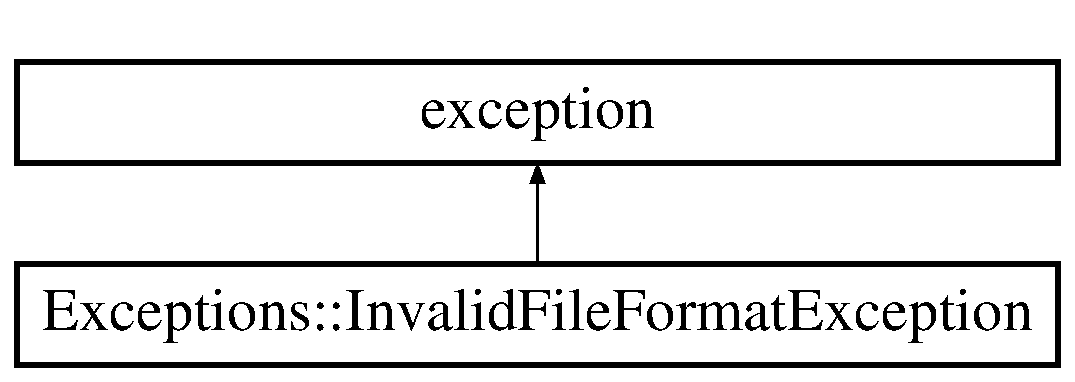
\includegraphics[height=2.000000cm]{class_exceptions_1_1_invalid_file_format_exception}
\end{center}
\end{figure}
\subsection*{Public Member Functions}
\begin{DoxyCompactItemize}
\item 
\hyperlink{class_exceptions_1_1_invalid_file_format_exception_a7696999598e515ba7fe761299d9f91a2}{Invalid\+File\+Format\+Exception} (const std\+::string \&\hyperlink{class_exceptions_1_1_invalid_file_format_exception_a7c035c95548acec2b3b3693cf746c1e2}{filename})
\item 
virtual const char $\ast$ \hyperlink{class_exceptions_1_1_invalid_file_format_exception_a31ecfcd73d0afb1e8c25e38a95b309b6}{what} () const   throw ()
\end{DoxyCompactItemize}
\subsection*{Private Attributes}
\begin{DoxyCompactItemize}
\item 
std\+::string \hyperlink{class_exceptions_1_1_invalid_file_format_exception_a7c035c95548acec2b3b3693cf746c1e2}{filename}
\end{DoxyCompactItemize}


\subsection{Constructor \& Destructor Documentation}
\hypertarget{class_exceptions_1_1_invalid_file_format_exception_a7696999598e515ba7fe761299d9f91a2}{}\index{Exceptions\+::\+Invalid\+File\+Format\+Exception@{Exceptions\+::\+Invalid\+File\+Format\+Exception}!Invalid\+File\+Format\+Exception@{Invalid\+File\+Format\+Exception}}
\index{Invalid\+File\+Format\+Exception@{Invalid\+File\+Format\+Exception}!Exceptions\+::\+Invalid\+File\+Format\+Exception@{Exceptions\+::\+Invalid\+File\+Format\+Exception}}
\subsubsection[{Invalid\+File\+Format\+Exception}]{\setlength{\rightskip}{0pt plus 5cm}Exceptions\+::\+Invalid\+File\+Format\+Exception\+::\+Invalid\+File\+Format\+Exception (
\begin{DoxyParamCaption}
\item[{const std\+::string \&}]{filename}
\end{DoxyParamCaption}
)\hspace{0.3cm}{\ttfamily [inline]}}\label{class_exceptions_1_1_invalid_file_format_exception_a7696999598e515ba7fe761299d9f91a2}


\subsection{Member Function Documentation}
\hypertarget{class_exceptions_1_1_invalid_file_format_exception_a31ecfcd73d0afb1e8c25e38a95b309b6}{}\index{Exceptions\+::\+Invalid\+File\+Format\+Exception@{Exceptions\+::\+Invalid\+File\+Format\+Exception}!what@{what}}
\index{what@{what}!Exceptions\+::\+Invalid\+File\+Format\+Exception@{Exceptions\+::\+Invalid\+File\+Format\+Exception}}
\subsubsection[{what}]{\setlength{\rightskip}{0pt plus 5cm}virtual const char$\ast$ Exceptions\+::\+Invalid\+File\+Format\+Exception\+::what (
\begin{DoxyParamCaption}
{}
\end{DoxyParamCaption}
) const throw  ) \hspace{0.3cm}{\ttfamily [inline]}, {\ttfamily [virtual]}}\label{class_exceptions_1_1_invalid_file_format_exception_a31ecfcd73d0afb1e8c25e38a95b309b6}


\subsection{Member Data Documentation}
\hypertarget{class_exceptions_1_1_invalid_file_format_exception_a7c035c95548acec2b3b3693cf746c1e2}{}\index{Exceptions\+::\+Invalid\+File\+Format\+Exception@{Exceptions\+::\+Invalid\+File\+Format\+Exception}!filename@{filename}}
\index{filename@{filename}!Exceptions\+::\+Invalid\+File\+Format\+Exception@{Exceptions\+::\+Invalid\+File\+Format\+Exception}}
\subsubsection[{filename}]{\setlength{\rightskip}{0pt plus 5cm}std\+::string Exceptions\+::\+Invalid\+File\+Format\+Exception\+::filename\hspace{0.3cm}{\ttfamily [private]}}\label{class_exceptions_1_1_invalid_file_format_exception_a7c035c95548acec2b3b3693cf746c1e2}


The documentation for this class was generated from the following file\+:\begin{DoxyCompactItemize}
\item 
src/exceptions/\hyperlink{invalid__file__format__exception_8h}{invalid\+\_\+file\+\_\+format\+\_\+exception.\+h}\end{DoxyCompactItemize}

\hypertarget{class_exceptions_1_1_invalid_filename_exception}{}\section{Exceptions\+:\+:Invalid\+Filename\+Exception Class Reference}
\label{class_exceptions_1_1_invalid_filename_exception}\index{Exceptions\+::\+Invalid\+Filename\+Exception@{Exceptions\+::\+Invalid\+Filename\+Exception}}


{\ttfamily \#include $<$invalid\+\_\+filename\+\_\+exception.\+h$>$}

Inheritance diagram for Exceptions\+:\+:Invalid\+Filename\+Exception\+:\begin{figure}[H]
\begin{center}
\leavevmode
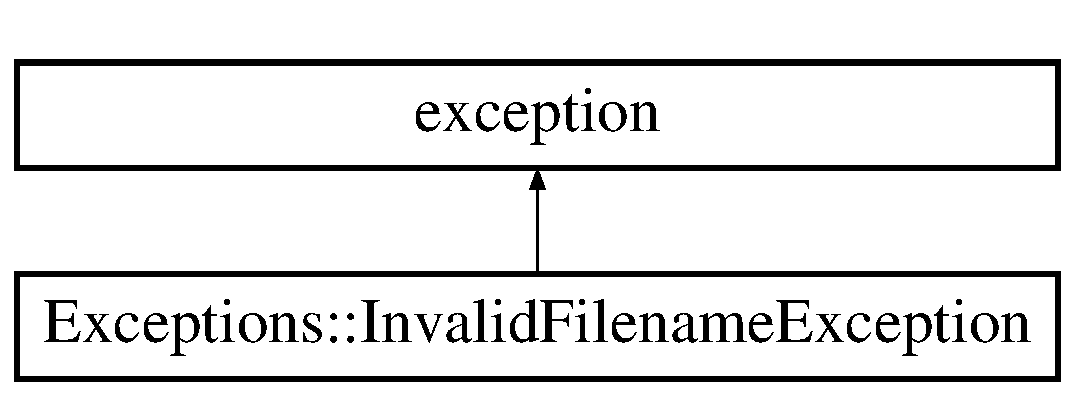
\includegraphics[height=2.000000cm]{class_exceptions_1_1_invalid_filename_exception}
\end{center}
\end{figure}
\subsection*{Public Member Functions}
\begin{DoxyCompactItemize}
\item 
\hyperlink{class_exceptions_1_1_invalid_filename_exception_aa931ab35f59e347af1b19322c02debe3}{Invalid\+Filename\+Exception} (const std\+::string \&\hyperlink{class_exceptions_1_1_invalid_filename_exception_a3c92e5e736e002495079a1537145549e}{filename})
\item 
virtual const char $\ast$ \hyperlink{class_exceptions_1_1_invalid_filename_exception_a4141ce1dc20a4cd02f82ea5a954f716d}{what} () const   throw ()
\end{DoxyCompactItemize}
\subsection*{Private Attributes}
\begin{DoxyCompactItemize}
\item 
std\+::string \hyperlink{class_exceptions_1_1_invalid_filename_exception_a3c92e5e736e002495079a1537145549e}{filename}
\end{DoxyCompactItemize}


\subsection{Constructor \& Destructor Documentation}
\hypertarget{class_exceptions_1_1_invalid_filename_exception_aa931ab35f59e347af1b19322c02debe3}{}\index{Exceptions\+::\+Invalid\+Filename\+Exception@{Exceptions\+::\+Invalid\+Filename\+Exception}!Invalid\+Filename\+Exception@{Invalid\+Filename\+Exception}}
\index{Invalid\+Filename\+Exception@{Invalid\+Filename\+Exception}!Exceptions\+::\+Invalid\+Filename\+Exception@{Exceptions\+::\+Invalid\+Filename\+Exception}}
\subsubsection[{Invalid\+Filename\+Exception}]{\setlength{\rightskip}{0pt plus 5cm}Exceptions\+::\+Invalid\+Filename\+Exception\+::\+Invalid\+Filename\+Exception (
\begin{DoxyParamCaption}
\item[{const std\+::string \&}]{filename}
\end{DoxyParamCaption}
)\hspace{0.3cm}{\ttfamily [inline]}}\label{class_exceptions_1_1_invalid_filename_exception_aa931ab35f59e347af1b19322c02debe3}


\subsection{Member Function Documentation}
\hypertarget{class_exceptions_1_1_invalid_filename_exception_a4141ce1dc20a4cd02f82ea5a954f716d}{}\index{Exceptions\+::\+Invalid\+Filename\+Exception@{Exceptions\+::\+Invalid\+Filename\+Exception}!what@{what}}
\index{what@{what}!Exceptions\+::\+Invalid\+Filename\+Exception@{Exceptions\+::\+Invalid\+Filename\+Exception}}
\subsubsection[{what}]{\setlength{\rightskip}{0pt plus 5cm}virtual const char$\ast$ Exceptions\+::\+Invalid\+Filename\+Exception\+::what (
\begin{DoxyParamCaption}
{}
\end{DoxyParamCaption}
) const throw  ) \hspace{0.3cm}{\ttfamily [inline]}, {\ttfamily [virtual]}}\label{class_exceptions_1_1_invalid_filename_exception_a4141ce1dc20a4cd02f82ea5a954f716d}


\subsection{Member Data Documentation}
\hypertarget{class_exceptions_1_1_invalid_filename_exception_a3c92e5e736e002495079a1537145549e}{}\index{Exceptions\+::\+Invalid\+Filename\+Exception@{Exceptions\+::\+Invalid\+Filename\+Exception}!filename@{filename}}
\index{filename@{filename}!Exceptions\+::\+Invalid\+Filename\+Exception@{Exceptions\+::\+Invalid\+Filename\+Exception}}
\subsubsection[{filename}]{\setlength{\rightskip}{0pt plus 5cm}std\+::string Exceptions\+::\+Invalid\+Filename\+Exception\+::filename\hspace{0.3cm}{\ttfamily [private]}}\label{class_exceptions_1_1_invalid_filename_exception_a3c92e5e736e002495079a1537145549e}


The documentation for this class was generated from the following file\+:\begin{DoxyCompactItemize}
\item 
src/exceptions/\hyperlink{invalid__filename__exception_8h}{invalid\+\_\+filename\+\_\+exception.\+h}\end{DoxyCompactItemize}

\hypertarget{class_exceptions_1_1_invalid_fragment_shader_exception}{}\section{Exceptions\+:\+:Invalid\+Fragment\+Shader\+Exception Class Reference}
\label{class_exceptions_1_1_invalid_fragment_shader_exception}\index{Exceptions\+::\+Invalid\+Fragment\+Shader\+Exception@{Exceptions\+::\+Invalid\+Fragment\+Shader\+Exception}}


{\ttfamily \#include $<$invalid\+\_\+fragment\+\_\+shader\+\_\+exception.\+h$>$}

Inheritance diagram for Exceptions\+:\+:Invalid\+Fragment\+Shader\+Exception\+:\begin{figure}[H]
\begin{center}
\leavevmode
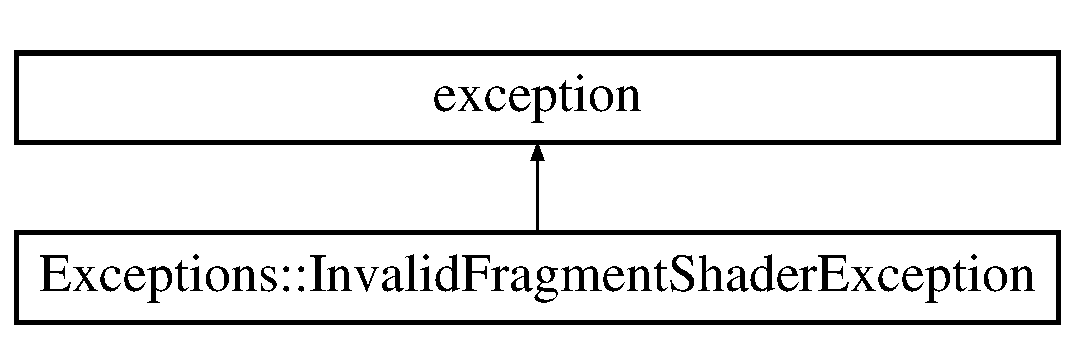
\includegraphics[height=2.000000cm]{class_exceptions_1_1_invalid_fragment_shader_exception}
\end{center}
\end{figure}
\subsection*{Public Member Functions}
\begin{DoxyCompactItemize}
\item 
\hyperlink{class_exceptions_1_1_invalid_fragment_shader_exception_adc23c55b308ae7ef93d03a6eee4bda31}{Invalid\+Fragment\+Shader\+Exception} (const unsigned int \hyperlink{class_exceptions_1_1_invalid_fragment_shader_exception_a3b2f1a947996d185b7a8a5c669ebbc74}{fragment\+\_\+shader\+\_\+binding})
\item 
virtual const char $\ast$ \hyperlink{class_exceptions_1_1_invalid_fragment_shader_exception_a816958e8042838f5a7ea88cefb4ea86c}{what} () const   throw ()
\end{DoxyCompactItemize}
\subsection*{Private Attributes}
\begin{DoxyCompactItemize}
\item 
unsigned int \hyperlink{class_exceptions_1_1_invalid_fragment_shader_exception_a3b2f1a947996d185b7a8a5c669ebbc74}{fragment\+\_\+shader\+\_\+binding}
\end{DoxyCompactItemize}


\subsection{Constructor \& Destructor Documentation}
\hypertarget{class_exceptions_1_1_invalid_fragment_shader_exception_adc23c55b308ae7ef93d03a6eee4bda31}{}\index{Exceptions\+::\+Invalid\+Fragment\+Shader\+Exception@{Exceptions\+::\+Invalid\+Fragment\+Shader\+Exception}!Invalid\+Fragment\+Shader\+Exception@{Invalid\+Fragment\+Shader\+Exception}}
\index{Invalid\+Fragment\+Shader\+Exception@{Invalid\+Fragment\+Shader\+Exception}!Exceptions\+::\+Invalid\+Fragment\+Shader\+Exception@{Exceptions\+::\+Invalid\+Fragment\+Shader\+Exception}}
\subsubsection[{Invalid\+Fragment\+Shader\+Exception}]{\setlength{\rightskip}{0pt plus 5cm}Exceptions\+::\+Invalid\+Fragment\+Shader\+Exception\+::\+Invalid\+Fragment\+Shader\+Exception (
\begin{DoxyParamCaption}
\item[{const unsigned int}]{fragment\+\_\+shader\+\_\+binding}
\end{DoxyParamCaption}
)\hspace{0.3cm}{\ttfamily [inline]}}\label{class_exceptions_1_1_invalid_fragment_shader_exception_adc23c55b308ae7ef93d03a6eee4bda31}


\subsection{Member Function Documentation}
\hypertarget{class_exceptions_1_1_invalid_fragment_shader_exception_a816958e8042838f5a7ea88cefb4ea86c}{}\index{Exceptions\+::\+Invalid\+Fragment\+Shader\+Exception@{Exceptions\+::\+Invalid\+Fragment\+Shader\+Exception}!what@{what}}
\index{what@{what}!Exceptions\+::\+Invalid\+Fragment\+Shader\+Exception@{Exceptions\+::\+Invalid\+Fragment\+Shader\+Exception}}
\subsubsection[{what}]{\setlength{\rightskip}{0pt plus 5cm}virtual const char$\ast$ Exceptions\+::\+Invalid\+Fragment\+Shader\+Exception\+::what (
\begin{DoxyParamCaption}
{}
\end{DoxyParamCaption}
) const throw  ) \hspace{0.3cm}{\ttfamily [inline]}, {\ttfamily [virtual]}}\label{class_exceptions_1_1_invalid_fragment_shader_exception_a816958e8042838f5a7ea88cefb4ea86c}


\subsection{Member Data Documentation}
\hypertarget{class_exceptions_1_1_invalid_fragment_shader_exception_a3b2f1a947996d185b7a8a5c669ebbc74}{}\index{Exceptions\+::\+Invalid\+Fragment\+Shader\+Exception@{Exceptions\+::\+Invalid\+Fragment\+Shader\+Exception}!fragment\+\_\+shader\+\_\+binding@{fragment\+\_\+shader\+\_\+binding}}
\index{fragment\+\_\+shader\+\_\+binding@{fragment\+\_\+shader\+\_\+binding}!Exceptions\+::\+Invalid\+Fragment\+Shader\+Exception@{Exceptions\+::\+Invalid\+Fragment\+Shader\+Exception}}
\subsubsection[{fragment\+\_\+shader\+\_\+binding}]{\setlength{\rightskip}{0pt plus 5cm}unsigned int Exceptions\+::\+Invalid\+Fragment\+Shader\+Exception\+::fragment\+\_\+shader\+\_\+binding\hspace{0.3cm}{\ttfamily [private]}}\label{class_exceptions_1_1_invalid_fragment_shader_exception_a3b2f1a947996d185b7a8a5c669ebbc74}


The documentation for this class was generated from the following file\+:\begin{DoxyCompactItemize}
\item 
src/exceptions/\hyperlink{invalid__fragment__shader__exception_8h}{invalid\+\_\+fragment\+\_\+shader\+\_\+exception.\+h}\end{DoxyCompactItemize}

\hypertarget{class_exceptions_1_1_invalid_geometry_shader_exception}{}\section{Exceptions\+:\+:Invalid\+Geometry\+Shader\+Exception Class Reference}
\label{class_exceptions_1_1_invalid_geometry_shader_exception}\index{Exceptions\+::\+Invalid\+Geometry\+Shader\+Exception@{Exceptions\+::\+Invalid\+Geometry\+Shader\+Exception}}


{\ttfamily \#include $<$invalid\+\_\+geometry\+\_\+shader\+\_\+exception.\+h$>$}

Inheritance diagram for Exceptions\+:\+:Invalid\+Geometry\+Shader\+Exception\+:\begin{figure}[H]
\begin{center}
\leavevmode
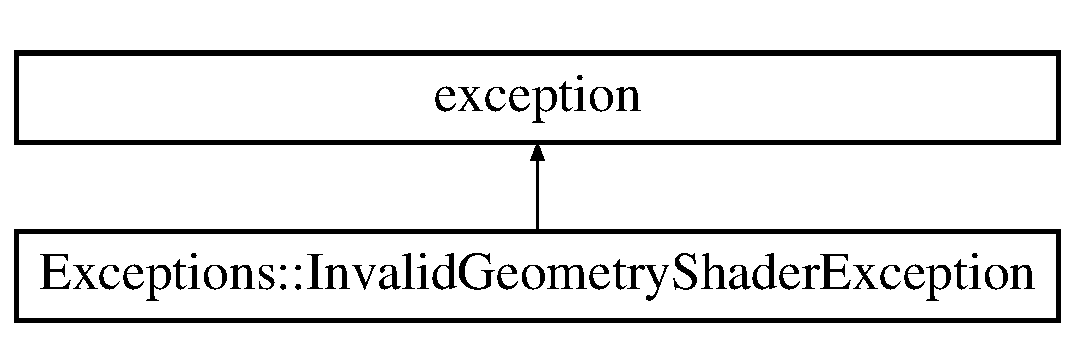
\includegraphics[height=2.000000cm]{class_exceptions_1_1_invalid_geometry_shader_exception}
\end{center}
\end{figure}
\subsection*{Public Member Functions}
\begin{DoxyCompactItemize}
\item 
\hyperlink{class_exceptions_1_1_invalid_geometry_shader_exception_abd1bf3f98bbb1a590d2d67e36b9d4b75}{Invalid\+Geometry\+Shader\+Exception} (const unsigned int \hyperlink{class_exceptions_1_1_invalid_geometry_shader_exception_a9b392c914b5d558b6ef0eaf130eb7ce9}{geometry\+\_\+shader\+\_\+binding})
\item 
virtual const char $\ast$ \hyperlink{class_exceptions_1_1_invalid_geometry_shader_exception_a9661fdb92878acabb635d02584005e81}{what} () const   throw ()
\end{DoxyCompactItemize}
\subsection*{Private Attributes}
\begin{DoxyCompactItemize}
\item 
unsigned int \hyperlink{class_exceptions_1_1_invalid_geometry_shader_exception_a9b392c914b5d558b6ef0eaf130eb7ce9}{geometry\+\_\+shader\+\_\+binding}
\end{DoxyCompactItemize}


\subsection{Constructor \& Destructor Documentation}
\hypertarget{class_exceptions_1_1_invalid_geometry_shader_exception_abd1bf3f98bbb1a590d2d67e36b9d4b75}{}\index{Exceptions\+::\+Invalid\+Geometry\+Shader\+Exception@{Exceptions\+::\+Invalid\+Geometry\+Shader\+Exception}!Invalid\+Geometry\+Shader\+Exception@{Invalid\+Geometry\+Shader\+Exception}}
\index{Invalid\+Geometry\+Shader\+Exception@{Invalid\+Geometry\+Shader\+Exception}!Exceptions\+::\+Invalid\+Geometry\+Shader\+Exception@{Exceptions\+::\+Invalid\+Geometry\+Shader\+Exception}}
\subsubsection[{Invalid\+Geometry\+Shader\+Exception}]{\setlength{\rightskip}{0pt plus 5cm}Exceptions\+::\+Invalid\+Geometry\+Shader\+Exception\+::\+Invalid\+Geometry\+Shader\+Exception (
\begin{DoxyParamCaption}
\item[{const unsigned int}]{geometry\+\_\+shader\+\_\+binding}
\end{DoxyParamCaption}
)\hspace{0.3cm}{\ttfamily [inline]}}\label{class_exceptions_1_1_invalid_geometry_shader_exception_abd1bf3f98bbb1a590d2d67e36b9d4b75}


\subsection{Member Function Documentation}
\hypertarget{class_exceptions_1_1_invalid_geometry_shader_exception_a9661fdb92878acabb635d02584005e81}{}\index{Exceptions\+::\+Invalid\+Geometry\+Shader\+Exception@{Exceptions\+::\+Invalid\+Geometry\+Shader\+Exception}!what@{what}}
\index{what@{what}!Exceptions\+::\+Invalid\+Geometry\+Shader\+Exception@{Exceptions\+::\+Invalid\+Geometry\+Shader\+Exception}}
\subsubsection[{what}]{\setlength{\rightskip}{0pt plus 5cm}virtual const char$\ast$ Exceptions\+::\+Invalid\+Geometry\+Shader\+Exception\+::what (
\begin{DoxyParamCaption}
{}
\end{DoxyParamCaption}
) const throw  ) \hspace{0.3cm}{\ttfamily [inline]}, {\ttfamily [virtual]}}\label{class_exceptions_1_1_invalid_geometry_shader_exception_a9661fdb92878acabb635d02584005e81}


\subsection{Member Data Documentation}
\hypertarget{class_exceptions_1_1_invalid_geometry_shader_exception_a9b392c914b5d558b6ef0eaf130eb7ce9}{}\index{Exceptions\+::\+Invalid\+Geometry\+Shader\+Exception@{Exceptions\+::\+Invalid\+Geometry\+Shader\+Exception}!geometry\+\_\+shader\+\_\+binding@{geometry\+\_\+shader\+\_\+binding}}
\index{geometry\+\_\+shader\+\_\+binding@{geometry\+\_\+shader\+\_\+binding}!Exceptions\+::\+Invalid\+Geometry\+Shader\+Exception@{Exceptions\+::\+Invalid\+Geometry\+Shader\+Exception}}
\subsubsection[{geometry\+\_\+shader\+\_\+binding}]{\setlength{\rightskip}{0pt plus 5cm}unsigned int Exceptions\+::\+Invalid\+Geometry\+Shader\+Exception\+::geometry\+\_\+shader\+\_\+binding\hspace{0.3cm}{\ttfamily [private]}}\label{class_exceptions_1_1_invalid_geometry_shader_exception_a9b392c914b5d558b6ef0eaf130eb7ce9}


The documentation for this class was generated from the following file\+:\begin{DoxyCompactItemize}
\item 
src/exceptions/\hyperlink{invalid__geometry__shader__exception_8h}{invalid\+\_\+geometry\+\_\+shader\+\_\+exception.\+h}\end{DoxyCompactItemize}

\hypertarget{class_exceptions_1_1_invalid_shader_name_exception}{}\section{Exceptions\+:\+:Invalid\+Shader\+Name\+Exception Class Reference}
\label{class_exceptions_1_1_invalid_shader_name_exception}\index{Exceptions\+::\+Invalid\+Shader\+Name\+Exception@{Exceptions\+::\+Invalid\+Shader\+Name\+Exception}}


{\ttfamily \#include $<$invalid\+\_\+shader\+\_\+name\+\_\+exception.\+h$>$}

Inheritance diagram for Exceptions\+:\+:Invalid\+Shader\+Name\+Exception\+:\begin{figure}[H]
\begin{center}
\leavevmode
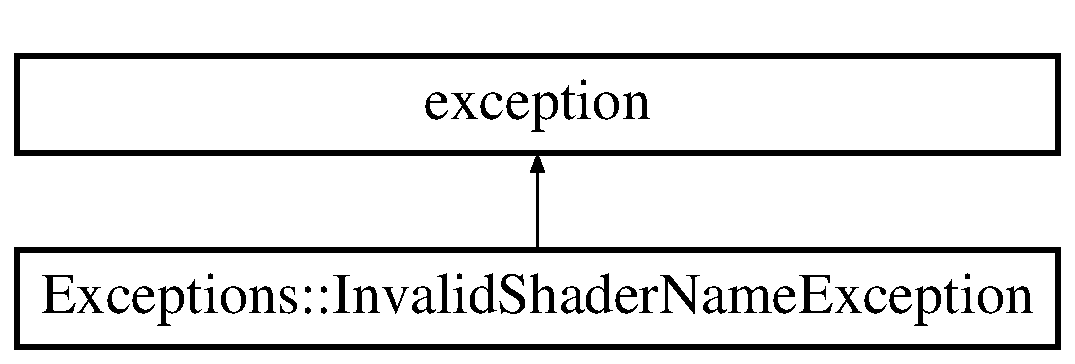
\includegraphics[height=2.000000cm]{class_exceptions_1_1_invalid_shader_name_exception}
\end{center}
\end{figure}
\subsection*{Public Member Functions}
\begin{DoxyCompactItemize}
\item 
\hyperlink{class_exceptions_1_1_invalid_shader_name_exception_a83014c98e72fb045d664a5af323ab023}{Invalid\+Shader\+Name\+Exception} (const std\+::string \&\hyperlink{class_exceptions_1_1_invalid_shader_name_exception_a3d9438219209a9bfe42df58f3107e3c8}{name})
\item 
virtual const char $\ast$ \hyperlink{class_exceptions_1_1_invalid_shader_name_exception_a8a01046b3d3cb4b8459d5f263c2c9295}{what} () const   throw ()
\end{DoxyCompactItemize}
\subsection*{Private Attributes}
\begin{DoxyCompactItemize}
\item 
std\+::string \hyperlink{class_exceptions_1_1_invalid_shader_name_exception_a3d9438219209a9bfe42df58f3107e3c8}{name}
\end{DoxyCompactItemize}


\subsection{Constructor \& Destructor Documentation}
\hypertarget{class_exceptions_1_1_invalid_shader_name_exception_a83014c98e72fb045d664a5af323ab023}{}\index{Exceptions\+::\+Invalid\+Shader\+Name\+Exception@{Exceptions\+::\+Invalid\+Shader\+Name\+Exception}!Invalid\+Shader\+Name\+Exception@{Invalid\+Shader\+Name\+Exception}}
\index{Invalid\+Shader\+Name\+Exception@{Invalid\+Shader\+Name\+Exception}!Exceptions\+::\+Invalid\+Shader\+Name\+Exception@{Exceptions\+::\+Invalid\+Shader\+Name\+Exception}}
\subsubsection[{Invalid\+Shader\+Name\+Exception}]{\setlength{\rightskip}{0pt plus 5cm}Exceptions\+::\+Invalid\+Shader\+Name\+Exception\+::\+Invalid\+Shader\+Name\+Exception (
\begin{DoxyParamCaption}
\item[{const std\+::string \&}]{name}
\end{DoxyParamCaption}
)\hspace{0.3cm}{\ttfamily [inline]}}\label{class_exceptions_1_1_invalid_shader_name_exception_a83014c98e72fb045d664a5af323ab023}


\subsection{Member Function Documentation}
\hypertarget{class_exceptions_1_1_invalid_shader_name_exception_a8a01046b3d3cb4b8459d5f263c2c9295}{}\index{Exceptions\+::\+Invalid\+Shader\+Name\+Exception@{Exceptions\+::\+Invalid\+Shader\+Name\+Exception}!what@{what}}
\index{what@{what}!Exceptions\+::\+Invalid\+Shader\+Name\+Exception@{Exceptions\+::\+Invalid\+Shader\+Name\+Exception}}
\subsubsection[{what}]{\setlength{\rightskip}{0pt plus 5cm}virtual const char$\ast$ Exceptions\+::\+Invalid\+Shader\+Name\+Exception\+::what (
\begin{DoxyParamCaption}
{}
\end{DoxyParamCaption}
) const throw  ) \hspace{0.3cm}{\ttfamily [inline]}, {\ttfamily [virtual]}}\label{class_exceptions_1_1_invalid_shader_name_exception_a8a01046b3d3cb4b8459d5f263c2c9295}


\subsection{Member Data Documentation}
\hypertarget{class_exceptions_1_1_invalid_shader_name_exception_a3d9438219209a9bfe42df58f3107e3c8}{}\index{Exceptions\+::\+Invalid\+Shader\+Name\+Exception@{Exceptions\+::\+Invalid\+Shader\+Name\+Exception}!name@{name}}
\index{name@{name}!Exceptions\+::\+Invalid\+Shader\+Name\+Exception@{Exceptions\+::\+Invalid\+Shader\+Name\+Exception}}
\subsubsection[{name}]{\setlength{\rightskip}{0pt plus 5cm}std\+::string Exceptions\+::\+Invalid\+Shader\+Name\+Exception\+::name\hspace{0.3cm}{\ttfamily [private]}}\label{class_exceptions_1_1_invalid_shader_name_exception_a3d9438219209a9bfe42df58f3107e3c8}


The documentation for this class was generated from the following file\+:\begin{DoxyCompactItemize}
\item 
src/exceptions/\hyperlink{invalid__shader__name__exception_8h}{invalid\+\_\+shader\+\_\+name\+\_\+exception.\+h}\end{DoxyCompactItemize}

\hypertarget{class_exceptions_1_1_invalid_shader_object_exception}{}\section{Exceptions\+:\+:Invalid\+Shader\+Object\+Exception Class Reference}
\label{class_exceptions_1_1_invalid_shader_object_exception}\index{Exceptions\+::\+Invalid\+Shader\+Object\+Exception@{Exceptions\+::\+Invalid\+Shader\+Object\+Exception}}


{\ttfamily \#include $<$invalid\+\_\+shader\+\_\+object\+\_\+exception.\+h$>$}

Inheritance diagram for Exceptions\+:\+:Invalid\+Shader\+Object\+Exception\+:\begin{figure}[H]
\begin{center}
\leavevmode
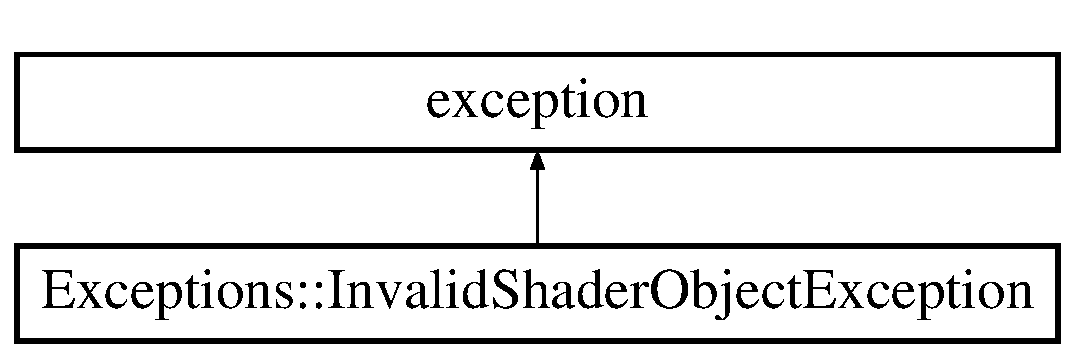
\includegraphics[height=2.000000cm]{class_exceptions_1_1_invalid_shader_object_exception}
\end{center}
\end{figure}
\subsection*{Public Member Functions}
\begin{DoxyCompactItemize}
\item 
\hyperlink{class_exceptions_1_1_invalid_shader_object_exception_a7de090bec61f4d09e95a6286a96e9f25}{Invalid\+Shader\+Object\+Exception} (const unsigned int \hyperlink{class_exceptions_1_1_invalid_shader_object_exception_a80365b85ba22f19254ea8e04cd0454e0}{shader\+\_\+object\+\_\+binding})
\item 
virtual const char $\ast$ \hyperlink{class_exceptions_1_1_invalid_shader_object_exception_a31caa1597313fbe9e166146b266087b0}{what} () const   throw ()
\end{DoxyCompactItemize}
\subsection*{Private Attributes}
\begin{DoxyCompactItemize}
\item 
unsigned int \hyperlink{class_exceptions_1_1_invalid_shader_object_exception_a80365b85ba22f19254ea8e04cd0454e0}{shader\+\_\+object\+\_\+binding}
\end{DoxyCompactItemize}


\subsection{Constructor \& Destructor Documentation}
\hypertarget{class_exceptions_1_1_invalid_shader_object_exception_a7de090bec61f4d09e95a6286a96e9f25}{}\index{Exceptions\+::\+Invalid\+Shader\+Object\+Exception@{Exceptions\+::\+Invalid\+Shader\+Object\+Exception}!Invalid\+Shader\+Object\+Exception@{Invalid\+Shader\+Object\+Exception}}
\index{Invalid\+Shader\+Object\+Exception@{Invalid\+Shader\+Object\+Exception}!Exceptions\+::\+Invalid\+Shader\+Object\+Exception@{Exceptions\+::\+Invalid\+Shader\+Object\+Exception}}
\subsubsection[{Invalid\+Shader\+Object\+Exception}]{\setlength{\rightskip}{0pt plus 5cm}Exceptions\+::\+Invalid\+Shader\+Object\+Exception\+::\+Invalid\+Shader\+Object\+Exception (
\begin{DoxyParamCaption}
\item[{const unsigned int}]{shader\+\_\+object\+\_\+binding}
\end{DoxyParamCaption}
)\hspace{0.3cm}{\ttfamily [inline]}}\label{class_exceptions_1_1_invalid_shader_object_exception_a7de090bec61f4d09e95a6286a96e9f25}


\subsection{Member Function Documentation}
\hypertarget{class_exceptions_1_1_invalid_shader_object_exception_a31caa1597313fbe9e166146b266087b0}{}\index{Exceptions\+::\+Invalid\+Shader\+Object\+Exception@{Exceptions\+::\+Invalid\+Shader\+Object\+Exception}!what@{what}}
\index{what@{what}!Exceptions\+::\+Invalid\+Shader\+Object\+Exception@{Exceptions\+::\+Invalid\+Shader\+Object\+Exception}}
\subsubsection[{what}]{\setlength{\rightskip}{0pt plus 5cm}virtual const char$\ast$ Exceptions\+::\+Invalid\+Shader\+Object\+Exception\+::what (
\begin{DoxyParamCaption}
{}
\end{DoxyParamCaption}
) const throw  ) \hspace{0.3cm}{\ttfamily [inline]}, {\ttfamily [virtual]}}\label{class_exceptions_1_1_invalid_shader_object_exception_a31caa1597313fbe9e166146b266087b0}


\subsection{Member Data Documentation}
\hypertarget{class_exceptions_1_1_invalid_shader_object_exception_a80365b85ba22f19254ea8e04cd0454e0}{}\index{Exceptions\+::\+Invalid\+Shader\+Object\+Exception@{Exceptions\+::\+Invalid\+Shader\+Object\+Exception}!shader\+\_\+object\+\_\+binding@{shader\+\_\+object\+\_\+binding}}
\index{shader\+\_\+object\+\_\+binding@{shader\+\_\+object\+\_\+binding}!Exceptions\+::\+Invalid\+Shader\+Object\+Exception@{Exceptions\+::\+Invalid\+Shader\+Object\+Exception}}
\subsubsection[{shader\+\_\+object\+\_\+binding}]{\setlength{\rightskip}{0pt plus 5cm}unsigned int Exceptions\+::\+Invalid\+Shader\+Object\+Exception\+::shader\+\_\+object\+\_\+binding\hspace{0.3cm}{\ttfamily [private]}}\label{class_exceptions_1_1_invalid_shader_object_exception_a80365b85ba22f19254ea8e04cd0454e0}


The documentation for this class was generated from the following file\+:\begin{DoxyCompactItemize}
\item 
src/exceptions/\hyperlink{invalid__shader__object__exception_8h}{invalid\+\_\+shader\+\_\+object\+\_\+exception.\+h}\end{DoxyCompactItemize}

\hypertarget{class_exceptions_1_1_invalid_shader_program_exception}{}\section{Exceptions\+:\+:Invalid\+Shader\+Program\+Exception Class Reference}
\label{class_exceptions_1_1_invalid_shader_program_exception}\index{Exceptions\+::\+Invalid\+Shader\+Program\+Exception@{Exceptions\+::\+Invalid\+Shader\+Program\+Exception}}


{\ttfamily \#include $<$invalid\+\_\+shader\+\_\+program\+\_\+exception.\+h$>$}

Inheritance diagram for Exceptions\+:\+:Invalid\+Shader\+Program\+Exception\+:\begin{figure}[H]
\begin{center}
\leavevmode
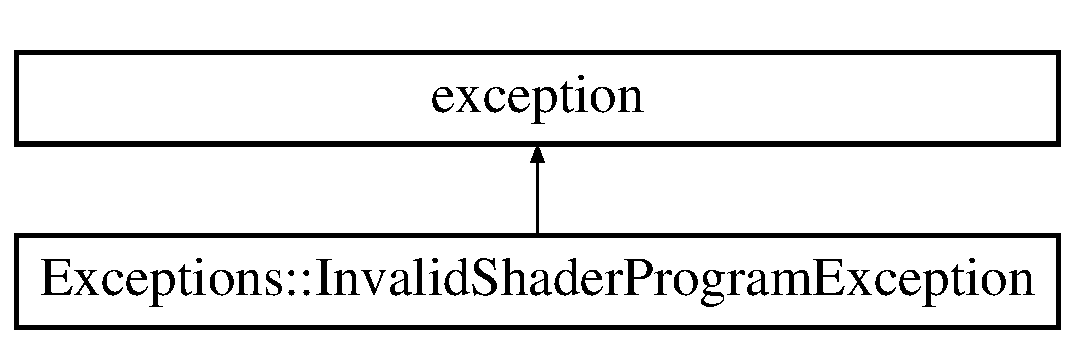
\includegraphics[height=2.000000cm]{class_exceptions_1_1_invalid_shader_program_exception}
\end{center}
\end{figure}
\subsection*{Public Member Functions}
\begin{DoxyCompactItemize}
\item 
\hyperlink{class_exceptions_1_1_invalid_shader_program_exception_aaa3d4fe606a35fd3ae882bf9e00da7c2}{Invalid\+Shader\+Program\+Exception} (const unsigned int \hyperlink{class_exceptions_1_1_invalid_shader_program_exception_ad04a0590a5111a7267ca56dc595efb28}{shader\+\_\+program})
\item 
virtual const char $\ast$ \hyperlink{class_exceptions_1_1_invalid_shader_program_exception_a5fc30a59b16fc5afae6211b289177ce8}{what} () const   throw ()
\end{DoxyCompactItemize}
\subsection*{Private Attributes}
\begin{DoxyCompactItemize}
\item 
unsigned int \hyperlink{class_exceptions_1_1_invalid_shader_program_exception_ad04a0590a5111a7267ca56dc595efb28}{shader\+\_\+program}
\end{DoxyCompactItemize}


\subsection{Constructor \& Destructor Documentation}
\hypertarget{class_exceptions_1_1_invalid_shader_program_exception_aaa3d4fe606a35fd3ae882bf9e00da7c2}{}\index{Exceptions\+::\+Invalid\+Shader\+Program\+Exception@{Exceptions\+::\+Invalid\+Shader\+Program\+Exception}!Invalid\+Shader\+Program\+Exception@{Invalid\+Shader\+Program\+Exception}}
\index{Invalid\+Shader\+Program\+Exception@{Invalid\+Shader\+Program\+Exception}!Exceptions\+::\+Invalid\+Shader\+Program\+Exception@{Exceptions\+::\+Invalid\+Shader\+Program\+Exception}}
\subsubsection[{Invalid\+Shader\+Program\+Exception}]{\setlength{\rightskip}{0pt plus 5cm}Exceptions\+::\+Invalid\+Shader\+Program\+Exception\+::\+Invalid\+Shader\+Program\+Exception (
\begin{DoxyParamCaption}
\item[{const unsigned int}]{shader\+\_\+program}
\end{DoxyParamCaption}
)\hspace{0.3cm}{\ttfamily [inline]}}\label{class_exceptions_1_1_invalid_shader_program_exception_aaa3d4fe606a35fd3ae882bf9e00da7c2}


\subsection{Member Function Documentation}
\hypertarget{class_exceptions_1_1_invalid_shader_program_exception_a5fc30a59b16fc5afae6211b289177ce8}{}\index{Exceptions\+::\+Invalid\+Shader\+Program\+Exception@{Exceptions\+::\+Invalid\+Shader\+Program\+Exception}!what@{what}}
\index{what@{what}!Exceptions\+::\+Invalid\+Shader\+Program\+Exception@{Exceptions\+::\+Invalid\+Shader\+Program\+Exception}}
\subsubsection[{what}]{\setlength{\rightskip}{0pt plus 5cm}virtual const char$\ast$ Exceptions\+::\+Invalid\+Shader\+Program\+Exception\+::what (
\begin{DoxyParamCaption}
{}
\end{DoxyParamCaption}
) const throw  ) \hspace{0.3cm}{\ttfamily [inline]}, {\ttfamily [virtual]}}\label{class_exceptions_1_1_invalid_shader_program_exception_a5fc30a59b16fc5afae6211b289177ce8}


\subsection{Member Data Documentation}
\hypertarget{class_exceptions_1_1_invalid_shader_program_exception_ad04a0590a5111a7267ca56dc595efb28}{}\index{Exceptions\+::\+Invalid\+Shader\+Program\+Exception@{Exceptions\+::\+Invalid\+Shader\+Program\+Exception}!shader\+\_\+program@{shader\+\_\+program}}
\index{shader\+\_\+program@{shader\+\_\+program}!Exceptions\+::\+Invalid\+Shader\+Program\+Exception@{Exceptions\+::\+Invalid\+Shader\+Program\+Exception}}
\subsubsection[{shader\+\_\+program}]{\setlength{\rightskip}{0pt plus 5cm}unsigned int Exceptions\+::\+Invalid\+Shader\+Program\+Exception\+::shader\+\_\+program\hspace{0.3cm}{\ttfamily [private]}}\label{class_exceptions_1_1_invalid_shader_program_exception_ad04a0590a5111a7267ca56dc595efb28}


The documentation for this class was generated from the following file\+:\begin{DoxyCompactItemize}
\item 
src/exceptions/\hyperlink{invalid__shader__program__exception_8h}{invalid\+\_\+shader\+\_\+program\+\_\+exception.\+h}\end{DoxyCompactItemize}

\hypertarget{class_exceptions_1_1_invalid_texture_name_exception}{}\section{Exceptions\+:\+:Invalid\+Texture\+Name\+Exception Class Reference}
\label{class_exceptions_1_1_invalid_texture_name_exception}\index{Exceptions\+::\+Invalid\+Texture\+Name\+Exception@{Exceptions\+::\+Invalid\+Texture\+Name\+Exception}}


{\ttfamily \#include $<$invalid\+\_\+texture\+\_\+name\+\_\+exception.\+h$>$}

Inheritance diagram for Exceptions\+:\+:Invalid\+Texture\+Name\+Exception\+:\begin{figure}[H]
\begin{center}
\leavevmode
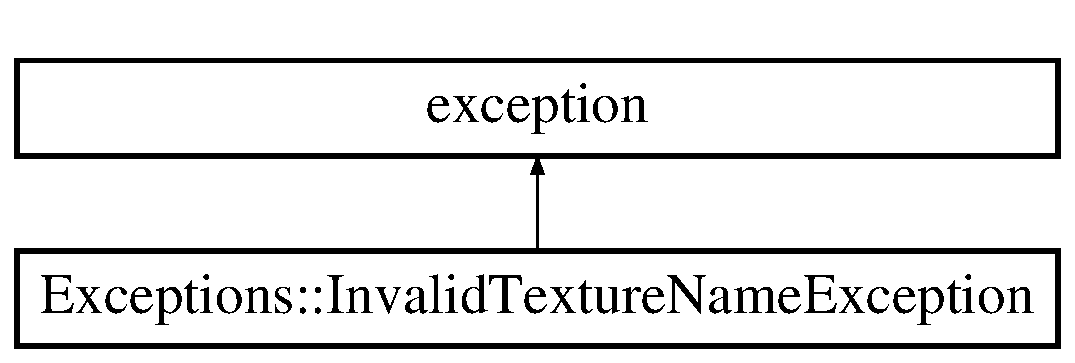
\includegraphics[height=2.000000cm]{class_exceptions_1_1_invalid_texture_name_exception}
\end{center}
\end{figure}
\subsection*{Public Member Functions}
\begin{DoxyCompactItemize}
\item 
\hyperlink{class_exceptions_1_1_invalid_texture_name_exception_a199fa95644139d5f439512588a7dca11}{Invalid\+Texture\+Name\+Exception} (const std\+::string \&\hyperlink{class_exceptions_1_1_invalid_texture_name_exception_a01142eb79f940de4fb5989df146716f1}{name})
\item 
virtual const char $\ast$ \hyperlink{class_exceptions_1_1_invalid_texture_name_exception_aabe515c7a32d71fa42951c0b1e0eaf14}{what} () const   throw ()
\end{DoxyCompactItemize}
\subsection*{Private Attributes}
\begin{DoxyCompactItemize}
\item 
std\+::string \hyperlink{class_exceptions_1_1_invalid_texture_name_exception_a01142eb79f940de4fb5989df146716f1}{name}
\end{DoxyCompactItemize}


\subsection{Constructor \& Destructor Documentation}
\hypertarget{class_exceptions_1_1_invalid_texture_name_exception_a199fa95644139d5f439512588a7dca11}{}\index{Exceptions\+::\+Invalid\+Texture\+Name\+Exception@{Exceptions\+::\+Invalid\+Texture\+Name\+Exception}!Invalid\+Texture\+Name\+Exception@{Invalid\+Texture\+Name\+Exception}}
\index{Invalid\+Texture\+Name\+Exception@{Invalid\+Texture\+Name\+Exception}!Exceptions\+::\+Invalid\+Texture\+Name\+Exception@{Exceptions\+::\+Invalid\+Texture\+Name\+Exception}}
\subsubsection[{Invalid\+Texture\+Name\+Exception}]{\setlength{\rightskip}{0pt plus 5cm}Exceptions\+::\+Invalid\+Texture\+Name\+Exception\+::\+Invalid\+Texture\+Name\+Exception (
\begin{DoxyParamCaption}
\item[{const std\+::string \&}]{name}
\end{DoxyParamCaption}
)\hspace{0.3cm}{\ttfamily [inline]}}\label{class_exceptions_1_1_invalid_texture_name_exception_a199fa95644139d5f439512588a7dca11}


\subsection{Member Function Documentation}
\hypertarget{class_exceptions_1_1_invalid_texture_name_exception_aabe515c7a32d71fa42951c0b1e0eaf14}{}\index{Exceptions\+::\+Invalid\+Texture\+Name\+Exception@{Exceptions\+::\+Invalid\+Texture\+Name\+Exception}!what@{what}}
\index{what@{what}!Exceptions\+::\+Invalid\+Texture\+Name\+Exception@{Exceptions\+::\+Invalid\+Texture\+Name\+Exception}}
\subsubsection[{what}]{\setlength{\rightskip}{0pt plus 5cm}virtual const char$\ast$ Exceptions\+::\+Invalid\+Texture\+Name\+Exception\+::what (
\begin{DoxyParamCaption}
{}
\end{DoxyParamCaption}
) const throw  ) \hspace{0.3cm}{\ttfamily [inline]}, {\ttfamily [virtual]}}\label{class_exceptions_1_1_invalid_texture_name_exception_aabe515c7a32d71fa42951c0b1e0eaf14}


\subsection{Member Data Documentation}
\hypertarget{class_exceptions_1_1_invalid_texture_name_exception_a01142eb79f940de4fb5989df146716f1}{}\index{Exceptions\+::\+Invalid\+Texture\+Name\+Exception@{Exceptions\+::\+Invalid\+Texture\+Name\+Exception}!name@{name}}
\index{name@{name}!Exceptions\+::\+Invalid\+Texture\+Name\+Exception@{Exceptions\+::\+Invalid\+Texture\+Name\+Exception}}
\subsubsection[{name}]{\setlength{\rightskip}{0pt plus 5cm}std\+::string Exceptions\+::\+Invalid\+Texture\+Name\+Exception\+::name\hspace{0.3cm}{\ttfamily [private]}}\label{class_exceptions_1_1_invalid_texture_name_exception_a01142eb79f940de4fb5989df146716f1}


The documentation for this class was generated from the following file\+:\begin{DoxyCompactItemize}
\item 
src/exceptions/\hyperlink{invalid__texture__name__exception_8h}{invalid\+\_\+texture\+\_\+name\+\_\+exception.\+h}\end{DoxyCompactItemize}

\hypertarget{class_exceptions_1_1_invalid_uniform_name_exception}{}\section{Exceptions\+:\+:Invalid\+Uniform\+Name\+Exception Class Reference}
\label{class_exceptions_1_1_invalid_uniform_name_exception}\index{Exceptions\+::\+Invalid\+Uniform\+Name\+Exception@{Exceptions\+::\+Invalid\+Uniform\+Name\+Exception}}


{\ttfamily \#include $<$invalid\+\_\+uniform\+\_\+name\+\_\+exception.\+h$>$}

Inheritance diagram for Exceptions\+:\+:Invalid\+Uniform\+Name\+Exception\+:\begin{figure}[H]
\begin{center}
\leavevmode
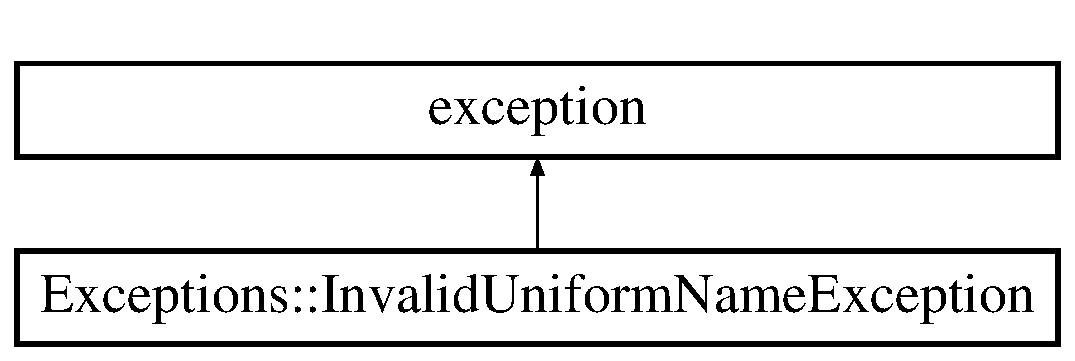
\includegraphics[height=2.000000cm]{class_exceptions_1_1_invalid_uniform_name_exception}
\end{center}
\end{figure}
\subsection*{Public Member Functions}
\begin{DoxyCompactItemize}
\item 
\hyperlink{class_exceptions_1_1_invalid_uniform_name_exception_a1eb355e5fbb46a511d5b94a6918eca31}{Invalid\+Uniform\+Name\+Exception} (const std\+::string \hyperlink{class_exceptions_1_1_invalid_uniform_name_exception_a6cb6b066c8b98fff6eb2c90da9aa1fb0}{name})
\item 
virtual const char $\ast$ \hyperlink{class_exceptions_1_1_invalid_uniform_name_exception_aca344333a94b1a1100d54d38392a109f}{what} () const   throw ()
\end{DoxyCompactItemize}
\subsection*{Private Attributes}
\begin{DoxyCompactItemize}
\item 
std\+::string \hyperlink{class_exceptions_1_1_invalid_uniform_name_exception_a6cb6b066c8b98fff6eb2c90da9aa1fb0}{name}
\end{DoxyCompactItemize}


\subsection{Constructor \& Destructor Documentation}
\hypertarget{class_exceptions_1_1_invalid_uniform_name_exception_a1eb355e5fbb46a511d5b94a6918eca31}{}\index{Exceptions\+::\+Invalid\+Uniform\+Name\+Exception@{Exceptions\+::\+Invalid\+Uniform\+Name\+Exception}!Invalid\+Uniform\+Name\+Exception@{Invalid\+Uniform\+Name\+Exception}}
\index{Invalid\+Uniform\+Name\+Exception@{Invalid\+Uniform\+Name\+Exception}!Exceptions\+::\+Invalid\+Uniform\+Name\+Exception@{Exceptions\+::\+Invalid\+Uniform\+Name\+Exception}}
\subsubsection[{Invalid\+Uniform\+Name\+Exception}]{\setlength{\rightskip}{0pt plus 5cm}Exceptions\+::\+Invalid\+Uniform\+Name\+Exception\+::\+Invalid\+Uniform\+Name\+Exception (
\begin{DoxyParamCaption}
\item[{const std\+::string}]{name}
\end{DoxyParamCaption}
)\hspace{0.3cm}{\ttfamily [inline]}}\label{class_exceptions_1_1_invalid_uniform_name_exception_a1eb355e5fbb46a511d5b94a6918eca31}


\subsection{Member Function Documentation}
\hypertarget{class_exceptions_1_1_invalid_uniform_name_exception_aca344333a94b1a1100d54d38392a109f}{}\index{Exceptions\+::\+Invalid\+Uniform\+Name\+Exception@{Exceptions\+::\+Invalid\+Uniform\+Name\+Exception}!what@{what}}
\index{what@{what}!Exceptions\+::\+Invalid\+Uniform\+Name\+Exception@{Exceptions\+::\+Invalid\+Uniform\+Name\+Exception}}
\subsubsection[{what}]{\setlength{\rightskip}{0pt plus 5cm}virtual const char$\ast$ Exceptions\+::\+Invalid\+Uniform\+Name\+Exception\+::what (
\begin{DoxyParamCaption}
{}
\end{DoxyParamCaption}
) const throw  ) \hspace{0.3cm}{\ttfamily [inline]}, {\ttfamily [virtual]}}\label{class_exceptions_1_1_invalid_uniform_name_exception_aca344333a94b1a1100d54d38392a109f}


\subsection{Member Data Documentation}
\hypertarget{class_exceptions_1_1_invalid_uniform_name_exception_a6cb6b066c8b98fff6eb2c90da9aa1fb0}{}\index{Exceptions\+::\+Invalid\+Uniform\+Name\+Exception@{Exceptions\+::\+Invalid\+Uniform\+Name\+Exception}!name@{name}}
\index{name@{name}!Exceptions\+::\+Invalid\+Uniform\+Name\+Exception@{Exceptions\+::\+Invalid\+Uniform\+Name\+Exception}}
\subsubsection[{name}]{\setlength{\rightskip}{0pt plus 5cm}std\+::string Exceptions\+::\+Invalid\+Uniform\+Name\+Exception\+::name\hspace{0.3cm}{\ttfamily [private]}}\label{class_exceptions_1_1_invalid_uniform_name_exception_a6cb6b066c8b98fff6eb2c90da9aa1fb0}


The documentation for this class was generated from the following file\+:\begin{DoxyCompactItemize}
\item 
src/exceptions/\hyperlink{invalid__uniform__name__exception_8h}{invalid\+\_\+uniform\+\_\+name\+\_\+exception.\+h}\end{DoxyCompactItemize}

\hypertarget{class_exceptions_1_1_invalid_vertex_array_exception}{}\section{Exceptions\+:\+:Invalid\+Vertex\+Array\+Exception Class Reference}
\label{class_exceptions_1_1_invalid_vertex_array_exception}\index{Exceptions\+::\+Invalid\+Vertex\+Array\+Exception@{Exceptions\+::\+Invalid\+Vertex\+Array\+Exception}}


{\ttfamily \#include $<$invalid\+\_\+vertex\+\_\+array\+\_\+exception.\+h$>$}

Inheritance diagram for Exceptions\+:\+:Invalid\+Vertex\+Array\+Exception\+:\begin{figure}[H]
\begin{center}
\leavevmode
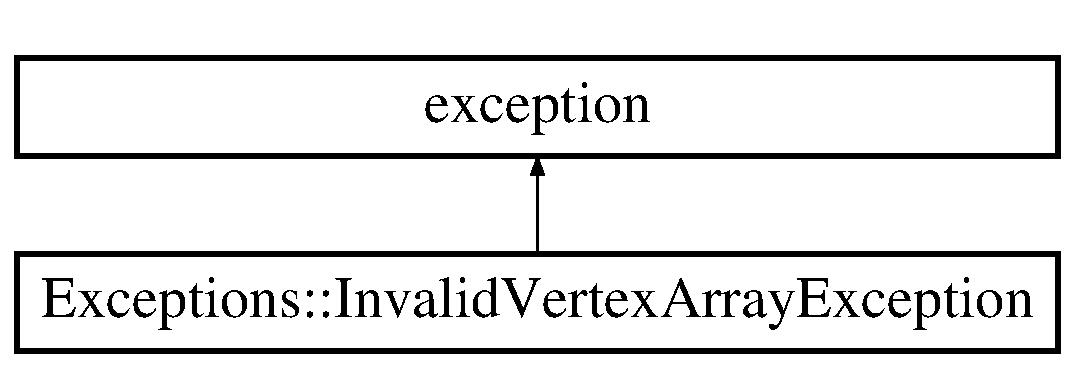
\includegraphics[height=2.000000cm]{class_exceptions_1_1_invalid_vertex_array_exception}
\end{center}
\end{figure}
\subsection*{Public Member Functions}
\begin{DoxyCompactItemize}
\item 
\hyperlink{class_exceptions_1_1_invalid_vertex_array_exception_a57cb1b8e280dc527308131a3409db516}{Invalid\+Vertex\+Array\+Exception} (const unsigned int \hyperlink{class_exceptions_1_1_invalid_vertex_array_exception_a600d7d65a0f48fe31c3de57a71766f1b}{vertex\+\_\+array\+\_\+binding})
\item 
virtual const char $\ast$ \hyperlink{class_exceptions_1_1_invalid_vertex_array_exception_a44652236482a680409b0db535c26bfa7}{what} () const   throw ()
\end{DoxyCompactItemize}
\subsection*{Private Attributes}
\begin{DoxyCompactItemize}
\item 
unsigned int \hyperlink{class_exceptions_1_1_invalid_vertex_array_exception_a600d7d65a0f48fe31c3de57a71766f1b}{vertex\+\_\+array\+\_\+binding}
\end{DoxyCompactItemize}


\subsection{Constructor \& Destructor Documentation}
\hypertarget{class_exceptions_1_1_invalid_vertex_array_exception_a57cb1b8e280dc527308131a3409db516}{}\index{Exceptions\+::\+Invalid\+Vertex\+Array\+Exception@{Exceptions\+::\+Invalid\+Vertex\+Array\+Exception}!Invalid\+Vertex\+Array\+Exception@{Invalid\+Vertex\+Array\+Exception}}
\index{Invalid\+Vertex\+Array\+Exception@{Invalid\+Vertex\+Array\+Exception}!Exceptions\+::\+Invalid\+Vertex\+Array\+Exception@{Exceptions\+::\+Invalid\+Vertex\+Array\+Exception}}
\subsubsection[{Invalid\+Vertex\+Array\+Exception}]{\setlength{\rightskip}{0pt plus 5cm}Exceptions\+::\+Invalid\+Vertex\+Array\+Exception\+::\+Invalid\+Vertex\+Array\+Exception (
\begin{DoxyParamCaption}
\item[{const unsigned int}]{vertex\+\_\+array\+\_\+binding}
\end{DoxyParamCaption}
)\hspace{0.3cm}{\ttfamily [inline]}}\label{class_exceptions_1_1_invalid_vertex_array_exception_a57cb1b8e280dc527308131a3409db516}


\subsection{Member Function Documentation}
\hypertarget{class_exceptions_1_1_invalid_vertex_array_exception_a44652236482a680409b0db535c26bfa7}{}\index{Exceptions\+::\+Invalid\+Vertex\+Array\+Exception@{Exceptions\+::\+Invalid\+Vertex\+Array\+Exception}!what@{what}}
\index{what@{what}!Exceptions\+::\+Invalid\+Vertex\+Array\+Exception@{Exceptions\+::\+Invalid\+Vertex\+Array\+Exception}}
\subsubsection[{what}]{\setlength{\rightskip}{0pt plus 5cm}virtual const char$\ast$ Exceptions\+::\+Invalid\+Vertex\+Array\+Exception\+::what (
\begin{DoxyParamCaption}
{}
\end{DoxyParamCaption}
) const throw  ) \hspace{0.3cm}{\ttfamily [inline]}, {\ttfamily [virtual]}}\label{class_exceptions_1_1_invalid_vertex_array_exception_a44652236482a680409b0db535c26bfa7}


\subsection{Member Data Documentation}
\hypertarget{class_exceptions_1_1_invalid_vertex_array_exception_a600d7d65a0f48fe31c3de57a71766f1b}{}\index{Exceptions\+::\+Invalid\+Vertex\+Array\+Exception@{Exceptions\+::\+Invalid\+Vertex\+Array\+Exception}!vertex\+\_\+array\+\_\+binding@{vertex\+\_\+array\+\_\+binding}}
\index{vertex\+\_\+array\+\_\+binding@{vertex\+\_\+array\+\_\+binding}!Exceptions\+::\+Invalid\+Vertex\+Array\+Exception@{Exceptions\+::\+Invalid\+Vertex\+Array\+Exception}}
\subsubsection[{vertex\+\_\+array\+\_\+binding}]{\setlength{\rightskip}{0pt plus 5cm}unsigned int Exceptions\+::\+Invalid\+Vertex\+Array\+Exception\+::vertex\+\_\+array\+\_\+binding\hspace{0.3cm}{\ttfamily [private]}}\label{class_exceptions_1_1_invalid_vertex_array_exception_a600d7d65a0f48fe31c3de57a71766f1b}


The documentation for this class was generated from the following file\+:\begin{DoxyCompactItemize}
\item 
src/exceptions/\hyperlink{invalid__vertex__array__exception_8h}{invalid\+\_\+vertex\+\_\+array\+\_\+exception.\+h}\end{DoxyCompactItemize}

\hypertarget{class_exceptions_1_1_invalid_vertex_shader_exception}{}\section{Exceptions\+:\+:Invalid\+Vertex\+Shader\+Exception Class Reference}
\label{class_exceptions_1_1_invalid_vertex_shader_exception}\index{Exceptions\+::\+Invalid\+Vertex\+Shader\+Exception@{Exceptions\+::\+Invalid\+Vertex\+Shader\+Exception}}


{\ttfamily \#include $<$invalid\+\_\+vertex\+\_\+shader\+\_\+exception.\+h$>$}

Inheritance diagram for Exceptions\+:\+:Invalid\+Vertex\+Shader\+Exception\+:\begin{figure}[H]
\begin{center}
\leavevmode
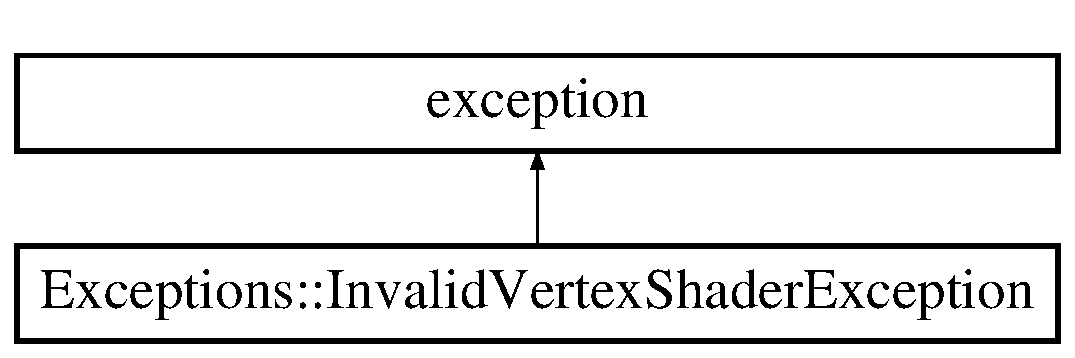
\includegraphics[height=2.000000cm]{class_exceptions_1_1_invalid_vertex_shader_exception}
\end{center}
\end{figure}
\subsection*{Public Member Functions}
\begin{DoxyCompactItemize}
\item 
\hyperlink{class_exceptions_1_1_invalid_vertex_shader_exception_a9ba81ea3e560d851ada643f0fdd8fefb}{Invalid\+Vertex\+Shader\+Exception} (const unsigned int \hyperlink{class_exceptions_1_1_invalid_vertex_shader_exception_a4bf93e6765dc1611a442cedc749ecb43}{vertex\+\_\+shader\+\_\+binding})
\item 
virtual const char $\ast$ \hyperlink{class_exceptions_1_1_invalid_vertex_shader_exception_a63b07be0e1e29b3f8f4c8f8cfb7eb735}{what} () const   throw ()
\end{DoxyCompactItemize}
\subsection*{Private Attributes}
\begin{DoxyCompactItemize}
\item 
unsigned int \hyperlink{class_exceptions_1_1_invalid_vertex_shader_exception_a4bf93e6765dc1611a442cedc749ecb43}{vertex\+\_\+shader\+\_\+binding}
\end{DoxyCompactItemize}


\subsection{Constructor \& Destructor Documentation}
\hypertarget{class_exceptions_1_1_invalid_vertex_shader_exception_a9ba81ea3e560d851ada643f0fdd8fefb}{}\index{Exceptions\+::\+Invalid\+Vertex\+Shader\+Exception@{Exceptions\+::\+Invalid\+Vertex\+Shader\+Exception}!Invalid\+Vertex\+Shader\+Exception@{Invalid\+Vertex\+Shader\+Exception}}
\index{Invalid\+Vertex\+Shader\+Exception@{Invalid\+Vertex\+Shader\+Exception}!Exceptions\+::\+Invalid\+Vertex\+Shader\+Exception@{Exceptions\+::\+Invalid\+Vertex\+Shader\+Exception}}
\subsubsection[{Invalid\+Vertex\+Shader\+Exception}]{\setlength{\rightskip}{0pt plus 5cm}Exceptions\+::\+Invalid\+Vertex\+Shader\+Exception\+::\+Invalid\+Vertex\+Shader\+Exception (
\begin{DoxyParamCaption}
\item[{const unsigned int}]{vertex\+\_\+shader\+\_\+binding}
\end{DoxyParamCaption}
)\hspace{0.3cm}{\ttfamily [inline]}}\label{class_exceptions_1_1_invalid_vertex_shader_exception_a9ba81ea3e560d851ada643f0fdd8fefb}


\subsection{Member Function Documentation}
\hypertarget{class_exceptions_1_1_invalid_vertex_shader_exception_a63b07be0e1e29b3f8f4c8f8cfb7eb735}{}\index{Exceptions\+::\+Invalid\+Vertex\+Shader\+Exception@{Exceptions\+::\+Invalid\+Vertex\+Shader\+Exception}!what@{what}}
\index{what@{what}!Exceptions\+::\+Invalid\+Vertex\+Shader\+Exception@{Exceptions\+::\+Invalid\+Vertex\+Shader\+Exception}}
\subsubsection[{what}]{\setlength{\rightskip}{0pt plus 5cm}virtual const char$\ast$ Exceptions\+::\+Invalid\+Vertex\+Shader\+Exception\+::what (
\begin{DoxyParamCaption}
{}
\end{DoxyParamCaption}
) const throw  ) \hspace{0.3cm}{\ttfamily [inline]}, {\ttfamily [virtual]}}\label{class_exceptions_1_1_invalid_vertex_shader_exception_a63b07be0e1e29b3f8f4c8f8cfb7eb735}


\subsection{Member Data Documentation}
\hypertarget{class_exceptions_1_1_invalid_vertex_shader_exception_a4bf93e6765dc1611a442cedc749ecb43}{}\index{Exceptions\+::\+Invalid\+Vertex\+Shader\+Exception@{Exceptions\+::\+Invalid\+Vertex\+Shader\+Exception}!vertex\+\_\+shader\+\_\+binding@{vertex\+\_\+shader\+\_\+binding}}
\index{vertex\+\_\+shader\+\_\+binding@{vertex\+\_\+shader\+\_\+binding}!Exceptions\+::\+Invalid\+Vertex\+Shader\+Exception@{Exceptions\+::\+Invalid\+Vertex\+Shader\+Exception}}
\subsubsection[{vertex\+\_\+shader\+\_\+binding}]{\setlength{\rightskip}{0pt plus 5cm}unsigned int Exceptions\+::\+Invalid\+Vertex\+Shader\+Exception\+::vertex\+\_\+shader\+\_\+binding\hspace{0.3cm}{\ttfamily [private]}}\label{class_exceptions_1_1_invalid_vertex_shader_exception_a4bf93e6765dc1611a442cedc749ecb43}


The documentation for this class was generated from the following file\+:\begin{DoxyCompactItemize}
\item 
src/exceptions/\hyperlink{invalid__vertex__shader__exception_8h}{invalid\+\_\+vertex\+\_\+shader\+\_\+exception.\+h}\end{DoxyCompactItemize}

\hypertarget{class_input_1_1_key_down_event}{}\section{Input\+:\+:Key\+Down\+Event Class Reference}
\label{class_input_1_1_key_down_event}\index{Input\+::\+Key\+Down\+Event@{Input\+::\+Key\+Down\+Event}}


{\ttfamily \#include $<$key\+\_\+down\+\_\+event.\+h$>$}

Inheritance diagram for Input\+:\+:Key\+Down\+Event\+:\begin{figure}[H]
\begin{center}
\leavevmode
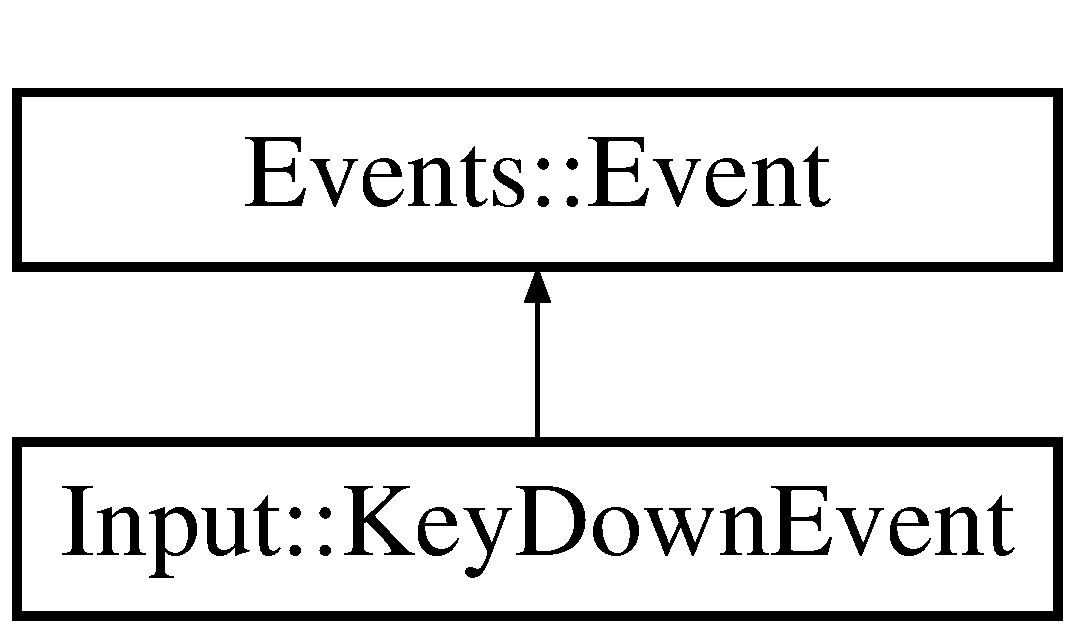
\includegraphics[height=2.000000cm]{class_input_1_1_key_down_event}
\end{center}
\end{figure}
\subsection*{Public Member Functions}
\begin{DoxyCompactItemize}
\item 
\hyperlink{class_input_1_1_key_down_event_a09a338e59c6ad57838e4b8b4624d44ad}{Key\+Down\+Event} (const int \hyperlink{class_input_1_1_key_down_event_ad1c8043b011c0398d398d61543ded8b4}{key})
\item 
const int \hyperlink{class_input_1_1_key_down_event_a12b8531b66c42248824afd19f8509269}{get\+Key} () const noexcept
\end{DoxyCompactItemize}
\subsection*{Private Attributes}
\begin{DoxyCompactItemize}
\item 
int \hyperlink{class_input_1_1_key_down_event_ad1c8043b011c0398d398d61543ded8b4}{key}
\end{DoxyCompactItemize}


\subsection{Constructor \& Destructor Documentation}
\hypertarget{class_input_1_1_key_down_event_a09a338e59c6ad57838e4b8b4624d44ad}{}\index{Input\+::\+Key\+Down\+Event@{Input\+::\+Key\+Down\+Event}!Key\+Down\+Event@{Key\+Down\+Event}}
\index{Key\+Down\+Event@{Key\+Down\+Event}!Input\+::\+Key\+Down\+Event@{Input\+::\+Key\+Down\+Event}}
\subsubsection[{Key\+Down\+Event}]{\setlength{\rightskip}{0pt plus 5cm}Input\+::\+Key\+Down\+Event\+::\+Key\+Down\+Event (
\begin{DoxyParamCaption}
\item[{const int}]{key}
\end{DoxyParamCaption}
)\hspace{0.3cm}{\ttfamily [inline]}}\label{class_input_1_1_key_down_event_a09a338e59c6ad57838e4b8b4624d44ad}


\subsection{Member Function Documentation}
\hypertarget{class_input_1_1_key_down_event_a12b8531b66c42248824afd19f8509269}{}\index{Input\+::\+Key\+Down\+Event@{Input\+::\+Key\+Down\+Event}!get\+Key@{get\+Key}}
\index{get\+Key@{get\+Key}!Input\+::\+Key\+Down\+Event@{Input\+::\+Key\+Down\+Event}}
\subsubsection[{get\+Key}]{\setlength{\rightskip}{0pt plus 5cm}const int Input\+::\+Key\+Down\+Event\+::get\+Key (
\begin{DoxyParamCaption}
{}
\end{DoxyParamCaption}
) const\hspace{0.3cm}{\ttfamily [inline]}, {\ttfamily [noexcept]}}\label{class_input_1_1_key_down_event_a12b8531b66c42248824afd19f8509269}


\subsection{Member Data Documentation}
\hypertarget{class_input_1_1_key_down_event_ad1c8043b011c0398d398d61543ded8b4}{}\index{Input\+::\+Key\+Down\+Event@{Input\+::\+Key\+Down\+Event}!key@{key}}
\index{key@{key}!Input\+::\+Key\+Down\+Event@{Input\+::\+Key\+Down\+Event}}
\subsubsection[{key}]{\setlength{\rightskip}{0pt plus 5cm}int Input\+::\+Key\+Down\+Event\+::key\hspace{0.3cm}{\ttfamily [private]}}\label{class_input_1_1_key_down_event_ad1c8043b011c0398d398d61543ded8b4}


The documentation for this class was generated from the following file\+:\begin{DoxyCompactItemize}
\item 
src/input/\hyperlink{key__down__event_8h}{key\+\_\+down\+\_\+event.\+h}\end{DoxyCompactItemize}

\hypertarget{class_input_1_1_key_up_event}{}\section{Input\+:\+:Key\+Up\+Event Class Reference}
\label{class_input_1_1_key_up_event}\index{Input\+::\+Key\+Up\+Event@{Input\+::\+Key\+Up\+Event}}


{\ttfamily \#include $<$key\+\_\+up\+\_\+event.\+h$>$}

Inheritance diagram for Input\+:\+:Key\+Up\+Event\+:\begin{figure}[H]
\begin{center}
\leavevmode
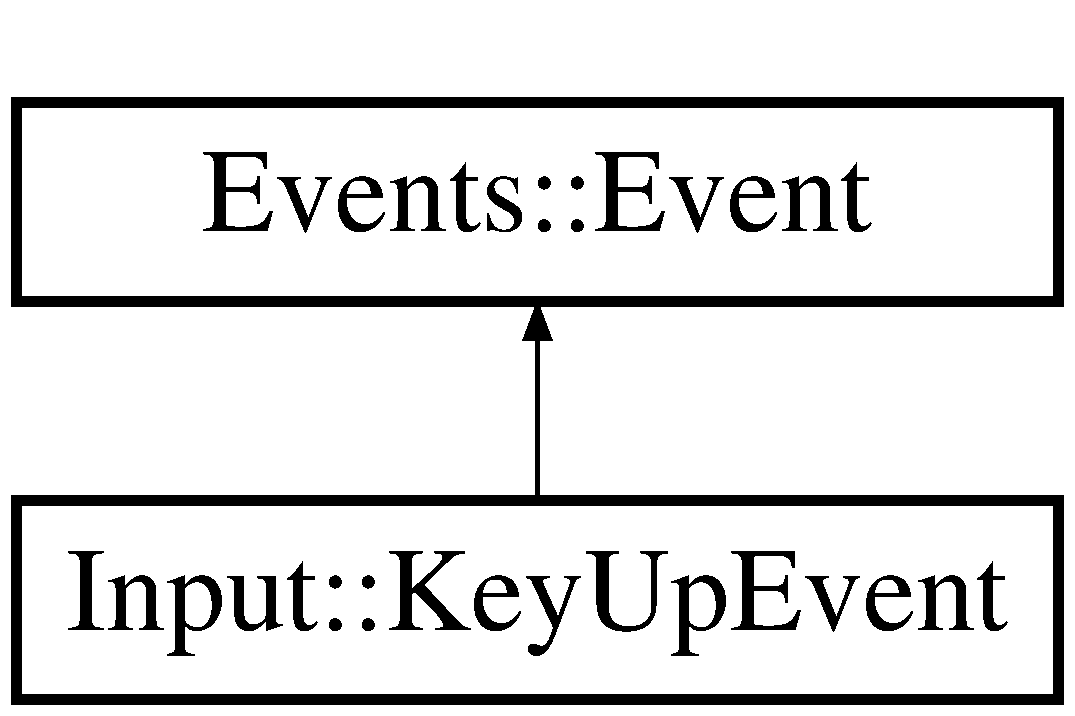
\includegraphics[height=2.000000cm]{class_input_1_1_key_up_event}
\end{center}
\end{figure}
\subsection*{Public Member Functions}
\begin{DoxyCompactItemize}
\item 
\hyperlink{class_input_1_1_key_up_event_ac1225d6a5d50d39fbb762a8639407876}{Key\+Up\+Event} (const int \hyperlink{class_input_1_1_key_up_event_a4be98a6c95e3ae7e5ad1c1702998b019}{key})
\item 
const int \hyperlink{class_input_1_1_key_up_event_a61f03fcd5c7577b5ffa13d912dd91cd7}{get\+Key} () const noexcept
\end{DoxyCompactItemize}
\subsection*{Private Attributes}
\begin{DoxyCompactItemize}
\item 
int \hyperlink{class_input_1_1_key_up_event_a4be98a6c95e3ae7e5ad1c1702998b019}{key}
\end{DoxyCompactItemize}


\subsection{Constructor \& Destructor Documentation}
\hypertarget{class_input_1_1_key_up_event_ac1225d6a5d50d39fbb762a8639407876}{}\index{Input\+::\+Key\+Up\+Event@{Input\+::\+Key\+Up\+Event}!Key\+Up\+Event@{Key\+Up\+Event}}
\index{Key\+Up\+Event@{Key\+Up\+Event}!Input\+::\+Key\+Up\+Event@{Input\+::\+Key\+Up\+Event}}
\subsubsection[{Key\+Up\+Event}]{\setlength{\rightskip}{0pt plus 5cm}Input\+::\+Key\+Up\+Event\+::\+Key\+Up\+Event (
\begin{DoxyParamCaption}
\item[{const int}]{key}
\end{DoxyParamCaption}
)\hspace{0.3cm}{\ttfamily [inline]}}\label{class_input_1_1_key_up_event_ac1225d6a5d50d39fbb762a8639407876}


\subsection{Member Function Documentation}
\hypertarget{class_input_1_1_key_up_event_a61f03fcd5c7577b5ffa13d912dd91cd7}{}\index{Input\+::\+Key\+Up\+Event@{Input\+::\+Key\+Up\+Event}!get\+Key@{get\+Key}}
\index{get\+Key@{get\+Key}!Input\+::\+Key\+Up\+Event@{Input\+::\+Key\+Up\+Event}}
\subsubsection[{get\+Key}]{\setlength{\rightskip}{0pt plus 5cm}const int Input\+::\+Key\+Up\+Event\+::get\+Key (
\begin{DoxyParamCaption}
{}
\end{DoxyParamCaption}
) const\hspace{0.3cm}{\ttfamily [inline]}, {\ttfamily [noexcept]}}\label{class_input_1_1_key_up_event_a61f03fcd5c7577b5ffa13d912dd91cd7}


\subsection{Member Data Documentation}
\hypertarget{class_input_1_1_key_up_event_a4be98a6c95e3ae7e5ad1c1702998b019}{}\index{Input\+::\+Key\+Up\+Event@{Input\+::\+Key\+Up\+Event}!key@{key}}
\index{key@{key}!Input\+::\+Key\+Up\+Event@{Input\+::\+Key\+Up\+Event}}
\subsubsection[{key}]{\setlength{\rightskip}{0pt plus 5cm}int Input\+::\+Key\+Up\+Event\+::key\hspace{0.3cm}{\ttfamily [private]}}\label{class_input_1_1_key_up_event_a4be98a6c95e3ae7e5ad1c1702998b019}


The documentation for this class was generated from the following file\+:\begin{DoxyCompactItemize}
\item 
src/input/\hyperlink{key__up__event_8h}{key\+\_\+up\+\_\+event.\+h}\end{DoxyCompactItemize}

\hypertarget{class_graphics_1_1_light}{}\section{Graphics\+:\+:Light Class Reference}
\label{class_graphics_1_1_light}\index{Graphics\+::\+Light@{Graphics\+::\+Light}}


{\ttfamily \#include $<$light.\+h$>$}

Inheritance diagram for Graphics\+:\+:Light\+:\begin{figure}[H]
\begin{center}
\leavevmode
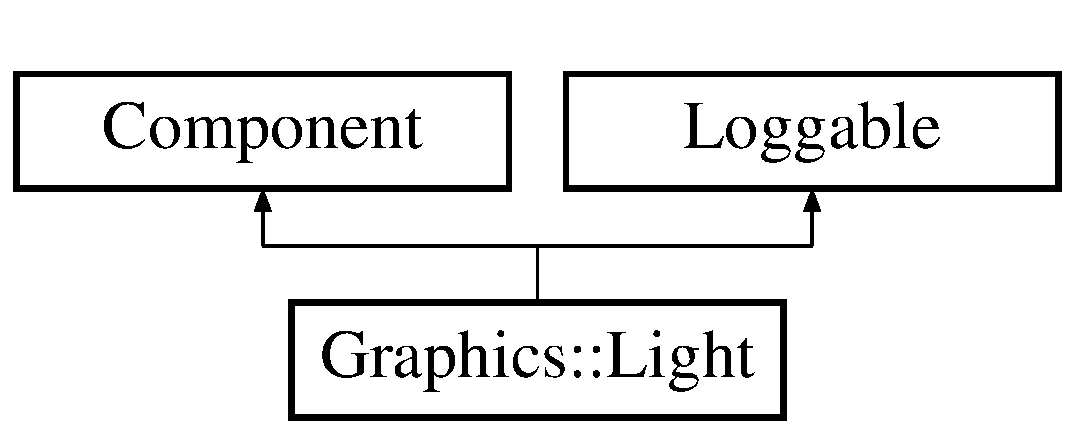
\includegraphics[height=2.000000cm]{class_graphics_1_1_light}
\end{center}
\end{figure}
\subsection*{Public Types}
\begin{DoxyCompactItemize}
\item 
enum \hyperlink{class_graphics_1_1_light_a6c3bc4c73b1bc4a96e0376be4ce0c007}{Type} \{ \hyperlink{class_graphics_1_1_light_a6c3bc4c73b1bc4a96e0376be4ce0c007aaebdbcb765394d25d6a604589a890f82}{Type\+::\+P\+O\+I\+N\+T}, 
\hyperlink{class_graphics_1_1_light_a6c3bc4c73b1bc4a96e0376be4ce0c007a5bac85a0c611ddef64ab0dfb383056f4}{Type\+::\+S\+P\+O\+T}
 \}
\end{DoxyCompactItemize}
\subsection*{Public Member Functions}
\begin{DoxyCompactItemize}
\item 
\hyperlink{class_graphics_1_1_light_ab15f626fee49a5332eac2f39ac6965f7}{Light} (const \hyperlink{class_graphics_1_1_light_a6c3bc4c73b1bc4a96e0376be4ce0c007}{Type} \&\hyperlink{class_graphics_1_1_light_a91b3331f89b6e025dfecfdc441a7080f}{type}=\hyperlink{class_graphics_1_1_light_a6c3bc4c73b1bc4a96e0376be4ce0c007aaebdbcb765394d25d6a604589a890f82}{Type\+::\+P\+O\+I\+N\+T})
\item 
\hyperlink{class_graphics_1_1_light_ad4ee718e1a005b54db45a660f3aaef00}{$\sim$\+Light} ()
\item 
virtual void \hyperlink{class_graphics_1_1_light_aa8ff320220d375edddae38daec0b3672}{on\+Start} () override
\item 
virtual const bool \hyperlink{class_graphics_1_1_light_ab208fc670894a75038b0e74a75816b21}{on\+Update} (const double delta) override
\item 
virtual void \hyperlink{class_graphics_1_1_light_a7d4ce913fcb79612a90937ae75b3ff2e}{on\+Destroy} () override
\item 
void \hyperlink{class_graphics_1_1_light_aff6f2b957a3a98ca5702ee078938c194}{set\+Color} (const glm\+::vec3 \hyperlink{class_graphics_1_1_light_a903bfd922e53ffe5df769d922928dd0e}{color}) noexcept
\item 
const glm\+::vec3 \hyperlink{class_graphics_1_1_light_a93b2736b7ccef7f7924c367c89a6a4d8}{get\+Color} () const noexcept
\item 
void \hyperlink{class_graphics_1_1_light_a90e92d6c4afa36b9dc8ef67e0b41bd0e}{set\+Intensity} (const float \hyperlink{class_graphics_1_1_light_a539a2fdf9981716b6c57a993262631f6}{intensity}) noexcept
\item 
const float \hyperlink{class_graphics_1_1_light_a5b56e9bd6fe8ddee31141ef867ea3198}{get\+Intensity} () const noexcept
\item 
void \hyperlink{class_graphics_1_1_light_ae0a3cf492daf5a8384474b147b99b540}{set\+Linear\+Attenuation} (const float linear) noexcept
\item 
const float \hyperlink{class_graphics_1_1_light_a2d9ccce40abbe0b728eab317ae7f2e6f}{get\+Linear\+Attenuation} () const noexcept
\item 
void \hyperlink{class_graphics_1_1_light_a6fbc065d5904745297c36e245da080f6}{set\+Quadratic\+Attenuation} (const float quadratic) noexcept
\item 
const float \hyperlink{class_graphics_1_1_light_aa3e34ad4fb661f2aa02c588d84c77173}{get\+Quadratic\+Attenuation} () const noexcept
\item 
const bool \hyperlink{class_graphics_1_1_light_a428cc9c8dbc7af11719417c5cad116ec}{casts\+Quantized\+Bands} () const noexcept
\item 
void \hyperlink{class_graphics_1_1_light_a65b266f9d2d3947ad0c57453e7df68bf}{set\+Number\+Of\+Quantized\+Bands} (const int bands) noexcept
\item 
const int \hyperlink{class_graphics_1_1_light_a008fca2c68899c80596f3fdcd61b5bfa}{get\+Number\+Of\+Quantized\+Bands} () const noexcept
\item 
void \hyperlink{class_graphics_1_1_light_a668d13ecfa976aea06da37ef74cc364b}{set\+Cone\+Angle} (const float angle) noexcept
\item 
const float \hyperlink{class_graphics_1_1_light_ac319eca9a1a6e9fe266f49d8b7424aa8}{get\+Cone\+Angle} () const noexcept
\item 
void \hyperlink{class_graphics_1_1_light_a1d4588fb18c81ef255ade5456b6a32f1}{set\+Cone\+Direction} (const glm\+::vec3 direction) noexcept
\item 
const glm\+::vec3 \hyperlink{class_graphics_1_1_light_aaf7c72aaa31711c07d44c530f89e29f6}{get\+Cone\+Direction} () const noexcept
\item 
const \hyperlink{class_graphics_1_1_light_a6c3bc4c73b1bc4a96e0376be4ce0c007}{Light\+::\+Type} \hyperlink{class_graphics_1_1_light_ad0ad78754ea7c205fa2dae8ad6c1d7b9}{get\+Type} () const noexcept
\item 
const float \hyperlink{class_graphics_1_1_light_a346c0e548fbec8de944642f638418a78}{influence\+On\+Component} (const \hyperlink{class_component}{Component} \&component) const 
\item 
virtual void \hyperlink{class_graphics_1_1_light_a2f6b15e75d42564f0db9dea75847a3e6}{log} (el\+::base\+::type\+::ostream\+\_\+t \&os) const 
\end{DoxyCompactItemize}
\subsection*{Static Public Member Functions}
\begin{DoxyCompactItemize}
\item 
static const \hyperlink{class_graphics_1_1_light_a6c3bc4c73b1bc4a96e0376be4ce0c007}{Light\+::\+Type} \hyperlink{class_graphics_1_1_light_a198ad8d3b143ca175cb201f79273bf24}{string\+To\+Type} (const std\+::string \&str)
\item 
static const std\+::string \hyperlink{class_graphics_1_1_light_a4dc16da5f94db88e73689064623b0bd7}{type\+To\+String} (const \hyperlink{class_graphics_1_1_light_a6c3bc4c73b1bc4a96e0376be4ce0c007}{Light\+::\+Type} \&\hyperlink{class_graphics_1_1_light_a91b3331f89b6e025dfecfdc441a7080f}{type})
\end{DoxyCompactItemize}
\subsection*{Private Attributes}
\begin{DoxyCompactItemize}
\item 
\hyperlink{class_graphics_1_1_light_a6c3bc4c73b1bc4a96e0376be4ce0c007}{Type} \hyperlink{class_graphics_1_1_light_a91b3331f89b6e025dfecfdc441a7080f}{type}
\item 
glm\+::vec3 \hyperlink{class_graphics_1_1_light_a903bfd922e53ffe5df769d922928dd0e}{color}
\item 
float \hyperlink{class_graphics_1_1_light_a539a2fdf9981716b6c57a993262631f6}{intensity}
\item 
float \hyperlink{class_graphics_1_1_light_a78d7dd2b77b0b982b68f9738e7c6b5d2}{linear\+\_\+attenuation}
\item 
float \hyperlink{class_graphics_1_1_light_a3820fefaee07fdfc1546a98e1365f2db}{quadratic\+\_\+attenuation}
\item 
int \hyperlink{class_graphics_1_1_light_a1188540a9957321d967d04dd6afec0f5}{quantized\+\_\+bands}
\item 
float \hyperlink{class_graphics_1_1_light_ac3f63577a382c18a9d8c3961df4008c9}{cone\+\_\+angle}
\item 
glm\+::vec3 \hyperlink{class_graphics_1_1_light_ac044f54135fdd638a0426e1e0ef9a63c}{cone\+\_\+direction}
\end{DoxyCompactItemize}
\subsection*{Additional Inherited Members}


\subsection{Member Enumeration Documentation}
\hypertarget{class_graphics_1_1_light_a6c3bc4c73b1bc4a96e0376be4ce0c007}{}\index{Graphics\+::\+Light@{Graphics\+::\+Light}!Type@{Type}}
\index{Type@{Type}!Graphics\+::\+Light@{Graphics\+::\+Light}}
\subsubsection[{Type}]{\setlength{\rightskip}{0pt plus 5cm}enum {\bf Graphics\+::\+Light\+::\+Type}\hspace{0.3cm}{\ttfamily [strong]}}\label{class_graphics_1_1_light_a6c3bc4c73b1bc4a96e0376be4ce0c007}
\begin{Desc}
\item[Enumerator]\par
\begin{description}
\index{P\+O\+I\+N\+T@{P\+O\+I\+N\+T}!Graphics\+::\+Light@{Graphics\+::\+Light}}\index{Graphics\+::\+Light@{Graphics\+::\+Light}!P\+O\+I\+N\+T@{P\+O\+I\+N\+T}}\item[{\em 
\hypertarget{class_graphics_1_1_light_a6c3bc4c73b1bc4a96e0376be4ce0c007aaebdbcb765394d25d6a604589a890f82}{}P\+O\+I\+N\+T\label{class_graphics_1_1_light_a6c3bc4c73b1bc4a96e0376be4ce0c007aaebdbcb765394d25d6a604589a890f82}
}]\index{S\+P\+O\+T@{S\+P\+O\+T}!Graphics\+::\+Light@{Graphics\+::\+Light}}\index{Graphics\+::\+Light@{Graphics\+::\+Light}!S\+P\+O\+T@{S\+P\+O\+T}}\item[{\em 
\hypertarget{class_graphics_1_1_light_a6c3bc4c73b1bc4a96e0376be4ce0c007a5bac85a0c611ddef64ab0dfb383056f4}{}S\+P\+O\+T\label{class_graphics_1_1_light_a6c3bc4c73b1bc4a96e0376be4ce0c007a5bac85a0c611ddef64ab0dfb383056f4}
}]\end{description}
\end{Desc}


\subsection{Constructor \& Destructor Documentation}
\hypertarget{class_graphics_1_1_light_ab15f626fee49a5332eac2f39ac6965f7}{}\index{Graphics\+::\+Light@{Graphics\+::\+Light}!Light@{Light}}
\index{Light@{Light}!Graphics\+::\+Light@{Graphics\+::\+Light}}
\subsubsection[{Light}]{\setlength{\rightskip}{0pt plus 5cm}Graphics\+::\+Light\+::\+Light (
\begin{DoxyParamCaption}
\item[{const {\bf Type} \&}]{type = {\ttfamily {\bf Type\+::\+P\+O\+I\+N\+T}}}
\end{DoxyParamCaption}
)}\label{class_graphics_1_1_light_ab15f626fee49a5332eac2f39ac6965f7}
\hypertarget{class_graphics_1_1_light_ad4ee718e1a005b54db45a660f3aaef00}{}\index{Graphics\+::\+Light@{Graphics\+::\+Light}!````~Light@{$\sim$\+Light}}
\index{````~Light@{$\sim$\+Light}!Graphics\+::\+Light@{Graphics\+::\+Light}}
\subsubsection[{$\sim$\+Light}]{\setlength{\rightskip}{0pt plus 5cm}Graphics\+::\+Light\+::$\sim$\+Light (
\begin{DoxyParamCaption}
{}
\end{DoxyParamCaption}
)}\label{class_graphics_1_1_light_ad4ee718e1a005b54db45a660f3aaef00}


\subsection{Member Function Documentation}
\hypertarget{class_graphics_1_1_light_a428cc9c8dbc7af11719417c5cad116ec}{}\index{Graphics\+::\+Light@{Graphics\+::\+Light}!casts\+Quantized\+Bands@{casts\+Quantized\+Bands}}
\index{casts\+Quantized\+Bands@{casts\+Quantized\+Bands}!Graphics\+::\+Light@{Graphics\+::\+Light}}
\subsubsection[{casts\+Quantized\+Bands}]{\setlength{\rightskip}{0pt plus 5cm}const bool Graphics\+::\+Light\+::casts\+Quantized\+Bands (
\begin{DoxyParamCaption}
{}
\end{DoxyParamCaption}
) const\hspace{0.3cm}{\ttfamily [noexcept]}}\label{class_graphics_1_1_light_a428cc9c8dbc7af11719417c5cad116ec}
\hypertarget{class_graphics_1_1_light_a93b2736b7ccef7f7924c367c89a6a4d8}{}\index{Graphics\+::\+Light@{Graphics\+::\+Light}!get\+Color@{get\+Color}}
\index{get\+Color@{get\+Color}!Graphics\+::\+Light@{Graphics\+::\+Light}}
\subsubsection[{get\+Color}]{\setlength{\rightskip}{0pt plus 5cm}const glm\+::vec3 Graphics\+::\+Light\+::get\+Color (
\begin{DoxyParamCaption}
{}
\end{DoxyParamCaption}
) const\hspace{0.3cm}{\ttfamily [noexcept]}}\label{class_graphics_1_1_light_a93b2736b7ccef7f7924c367c89a6a4d8}
\hypertarget{class_graphics_1_1_light_ac319eca9a1a6e9fe266f49d8b7424aa8}{}\index{Graphics\+::\+Light@{Graphics\+::\+Light}!get\+Cone\+Angle@{get\+Cone\+Angle}}
\index{get\+Cone\+Angle@{get\+Cone\+Angle}!Graphics\+::\+Light@{Graphics\+::\+Light}}
\subsubsection[{get\+Cone\+Angle}]{\setlength{\rightskip}{0pt plus 5cm}const float Graphics\+::\+Light\+::get\+Cone\+Angle (
\begin{DoxyParamCaption}
{}
\end{DoxyParamCaption}
) const\hspace{0.3cm}{\ttfamily [noexcept]}}\label{class_graphics_1_1_light_ac319eca9a1a6e9fe266f49d8b7424aa8}
\hypertarget{class_graphics_1_1_light_aaf7c72aaa31711c07d44c530f89e29f6}{}\index{Graphics\+::\+Light@{Graphics\+::\+Light}!get\+Cone\+Direction@{get\+Cone\+Direction}}
\index{get\+Cone\+Direction@{get\+Cone\+Direction}!Graphics\+::\+Light@{Graphics\+::\+Light}}
\subsubsection[{get\+Cone\+Direction}]{\setlength{\rightskip}{0pt plus 5cm}const glm\+::vec3 Graphics\+::\+Light\+::get\+Cone\+Direction (
\begin{DoxyParamCaption}
{}
\end{DoxyParamCaption}
) const\hspace{0.3cm}{\ttfamily [noexcept]}}\label{class_graphics_1_1_light_aaf7c72aaa31711c07d44c530f89e29f6}
\hypertarget{class_graphics_1_1_light_a5b56e9bd6fe8ddee31141ef867ea3198}{}\index{Graphics\+::\+Light@{Graphics\+::\+Light}!get\+Intensity@{get\+Intensity}}
\index{get\+Intensity@{get\+Intensity}!Graphics\+::\+Light@{Graphics\+::\+Light}}
\subsubsection[{get\+Intensity}]{\setlength{\rightskip}{0pt plus 5cm}const float Graphics\+::\+Light\+::get\+Intensity (
\begin{DoxyParamCaption}
{}
\end{DoxyParamCaption}
) const\hspace{0.3cm}{\ttfamily [noexcept]}}\label{class_graphics_1_1_light_a5b56e9bd6fe8ddee31141ef867ea3198}
\hypertarget{class_graphics_1_1_light_a2d9ccce40abbe0b728eab317ae7f2e6f}{}\index{Graphics\+::\+Light@{Graphics\+::\+Light}!get\+Linear\+Attenuation@{get\+Linear\+Attenuation}}
\index{get\+Linear\+Attenuation@{get\+Linear\+Attenuation}!Graphics\+::\+Light@{Graphics\+::\+Light}}
\subsubsection[{get\+Linear\+Attenuation}]{\setlength{\rightskip}{0pt plus 5cm}const float Graphics\+::\+Light\+::get\+Linear\+Attenuation (
\begin{DoxyParamCaption}
{}
\end{DoxyParamCaption}
) const\hspace{0.3cm}{\ttfamily [noexcept]}}\label{class_graphics_1_1_light_a2d9ccce40abbe0b728eab317ae7f2e6f}
\hypertarget{class_graphics_1_1_light_a008fca2c68899c80596f3fdcd61b5bfa}{}\index{Graphics\+::\+Light@{Graphics\+::\+Light}!get\+Number\+Of\+Quantized\+Bands@{get\+Number\+Of\+Quantized\+Bands}}
\index{get\+Number\+Of\+Quantized\+Bands@{get\+Number\+Of\+Quantized\+Bands}!Graphics\+::\+Light@{Graphics\+::\+Light}}
\subsubsection[{get\+Number\+Of\+Quantized\+Bands}]{\setlength{\rightskip}{0pt plus 5cm}const int Graphics\+::\+Light\+::get\+Number\+Of\+Quantized\+Bands (
\begin{DoxyParamCaption}
{}
\end{DoxyParamCaption}
) const\hspace{0.3cm}{\ttfamily [noexcept]}}\label{class_graphics_1_1_light_a008fca2c68899c80596f3fdcd61b5bfa}
\hypertarget{class_graphics_1_1_light_aa3e34ad4fb661f2aa02c588d84c77173}{}\index{Graphics\+::\+Light@{Graphics\+::\+Light}!get\+Quadratic\+Attenuation@{get\+Quadratic\+Attenuation}}
\index{get\+Quadratic\+Attenuation@{get\+Quadratic\+Attenuation}!Graphics\+::\+Light@{Graphics\+::\+Light}}
\subsubsection[{get\+Quadratic\+Attenuation}]{\setlength{\rightskip}{0pt plus 5cm}const float Graphics\+::\+Light\+::get\+Quadratic\+Attenuation (
\begin{DoxyParamCaption}
{}
\end{DoxyParamCaption}
) const\hspace{0.3cm}{\ttfamily [noexcept]}}\label{class_graphics_1_1_light_aa3e34ad4fb661f2aa02c588d84c77173}
\hypertarget{class_graphics_1_1_light_ad0ad78754ea7c205fa2dae8ad6c1d7b9}{}\index{Graphics\+::\+Light@{Graphics\+::\+Light}!get\+Type@{get\+Type}}
\index{get\+Type@{get\+Type}!Graphics\+::\+Light@{Graphics\+::\+Light}}
\subsubsection[{get\+Type}]{\setlength{\rightskip}{0pt plus 5cm}const {\bf Light\+::\+Type} Graphics\+::\+Light\+::get\+Type (
\begin{DoxyParamCaption}
{}
\end{DoxyParamCaption}
) const\hspace{0.3cm}{\ttfamily [noexcept]}}\label{class_graphics_1_1_light_ad0ad78754ea7c205fa2dae8ad6c1d7b9}
\hypertarget{class_graphics_1_1_light_a346c0e548fbec8de944642f638418a78}{}\index{Graphics\+::\+Light@{Graphics\+::\+Light}!influence\+On\+Component@{influence\+On\+Component}}
\index{influence\+On\+Component@{influence\+On\+Component}!Graphics\+::\+Light@{Graphics\+::\+Light}}
\subsubsection[{influence\+On\+Component}]{\setlength{\rightskip}{0pt plus 5cm}const float Graphics\+::\+Light\+::influence\+On\+Component (
\begin{DoxyParamCaption}
\item[{const {\bf Component} \&}]{component}
\end{DoxyParamCaption}
) const}\label{class_graphics_1_1_light_a346c0e548fbec8de944642f638418a78}
\hypertarget{class_graphics_1_1_light_a2f6b15e75d42564f0db9dea75847a3e6}{}\index{Graphics\+::\+Light@{Graphics\+::\+Light}!log@{log}}
\index{log@{log}!Graphics\+::\+Light@{Graphics\+::\+Light}}
\subsubsection[{log}]{\setlength{\rightskip}{0pt plus 5cm}void Graphics\+::\+Light\+::log (
\begin{DoxyParamCaption}
\item[{el\+::base\+::type\+::ostream\+\_\+t \&}]{os}
\end{DoxyParamCaption}
) const\hspace{0.3cm}{\ttfamily [virtual]}}\label{class_graphics_1_1_light_a2f6b15e75d42564f0db9dea75847a3e6}
\hypertarget{class_graphics_1_1_light_a7d4ce913fcb79612a90937ae75b3ff2e}{}\index{Graphics\+::\+Light@{Graphics\+::\+Light}!on\+Destroy@{on\+Destroy}}
\index{on\+Destroy@{on\+Destroy}!Graphics\+::\+Light@{Graphics\+::\+Light}}
\subsubsection[{on\+Destroy}]{\setlength{\rightskip}{0pt plus 5cm}void Graphics\+::\+Light\+::on\+Destroy (
\begin{DoxyParamCaption}
{}
\end{DoxyParamCaption}
)\hspace{0.3cm}{\ttfamily [override]}, {\ttfamily [virtual]}}\label{class_graphics_1_1_light_a7d4ce913fcb79612a90937ae75b3ff2e}


Implements \hyperlink{class_component_a2b198f27162a6caf63917e304295f892}{Component}.

\hypertarget{class_graphics_1_1_light_aa8ff320220d375edddae38daec0b3672}{}\index{Graphics\+::\+Light@{Graphics\+::\+Light}!on\+Start@{on\+Start}}
\index{on\+Start@{on\+Start}!Graphics\+::\+Light@{Graphics\+::\+Light}}
\subsubsection[{on\+Start}]{\setlength{\rightskip}{0pt plus 5cm}void Graphics\+::\+Light\+::on\+Start (
\begin{DoxyParamCaption}
{}
\end{DoxyParamCaption}
)\hspace{0.3cm}{\ttfamily [override]}, {\ttfamily [virtual]}}\label{class_graphics_1_1_light_aa8ff320220d375edddae38daec0b3672}


Implements \hyperlink{class_component_a4a528a8790dbc141ffd0aba638b6dcc4}{Component}.

\hypertarget{class_graphics_1_1_light_ab208fc670894a75038b0e74a75816b21}{}\index{Graphics\+::\+Light@{Graphics\+::\+Light}!on\+Update@{on\+Update}}
\index{on\+Update@{on\+Update}!Graphics\+::\+Light@{Graphics\+::\+Light}}
\subsubsection[{on\+Update}]{\setlength{\rightskip}{0pt plus 5cm}const bool Graphics\+::\+Light\+::on\+Update (
\begin{DoxyParamCaption}
\item[{const double}]{delta}
\end{DoxyParamCaption}
)\hspace{0.3cm}{\ttfamily [override]}, {\ttfamily [virtual]}}\label{class_graphics_1_1_light_ab208fc670894a75038b0e74a75816b21}


Implements \hyperlink{class_component_a8be284fccf4e97cee6705bd2d8f3705e}{Component}.

\hypertarget{class_graphics_1_1_light_aff6f2b957a3a98ca5702ee078938c194}{}\index{Graphics\+::\+Light@{Graphics\+::\+Light}!set\+Color@{set\+Color}}
\index{set\+Color@{set\+Color}!Graphics\+::\+Light@{Graphics\+::\+Light}}
\subsubsection[{set\+Color}]{\setlength{\rightskip}{0pt plus 5cm}void Graphics\+::\+Light\+::set\+Color (
\begin{DoxyParamCaption}
\item[{const glm\+::vec3}]{color}
\end{DoxyParamCaption}
)\hspace{0.3cm}{\ttfamily [noexcept]}}\label{class_graphics_1_1_light_aff6f2b957a3a98ca5702ee078938c194}
\hypertarget{class_graphics_1_1_light_a668d13ecfa976aea06da37ef74cc364b}{}\index{Graphics\+::\+Light@{Graphics\+::\+Light}!set\+Cone\+Angle@{set\+Cone\+Angle}}
\index{set\+Cone\+Angle@{set\+Cone\+Angle}!Graphics\+::\+Light@{Graphics\+::\+Light}}
\subsubsection[{set\+Cone\+Angle}]{\setlength{\rightskip}{0pt plus 5cm}void Graphics\+::\+Light\+::set\+Cone\+Angle (
\begin{DoxyParamCaption}
\item[{const float}]{angle}
\end{DoxyParamCaption}
)\hspace{0.3cm}{\ttfamily [noexcept]}}\label{class_graphics_1_1_light_a668d13ecfa976aea06da37ef74cc364b}
\hypertarget{class_graphics_1_1_light_a1d4588fb18c81ef255ade5456b6a32f1}{}\index{Graphics\+::\+Light@{Graphics\+::\+Light}!set\+Cone\+Direction@{set\+Cone\+Direction}}
\index{set\+Cone\+Direction@{set\+Cone\+Direction}!Graphics\+::\+Light@{Graphics\+::\+Light}}
\subsubsection[{set\+Cone\+Direction}]{\setlength{\rightskip}{0pt plus 5cm}void Graphics\+::\+Light\+::set\+Cone\+Direction (
\begin{DoxyParamCaption}
\item[{const glm\+::vec3}]{direction}
\end{DoxyParamCaption}
)\hspace{0.3cm}{\ttfamily [noexcept]}}\label{class_graphics_1_1_light_a1d4588fb18c81ef255ade5456b6a32f1}
\hypertarget{class_graphics_1_1_light_a90e92d6c4afa36b9dc8ef67e0b41bd0e}{}\index{Graphics\+::\+Light@{Graphics\+::\+Light}!set\+Intensity@{set\+Intensity}}
\index{set\+Intensity@{set\+Intensity}!Graphics\+::\+Light@{Graphics\+::\+Light}}
\subsubsection[{set\+Intensity}]{\setlength{\rightskip}{0pt plus 5cm}void Graphics\+::\+Light\+::set\+Intensity (
\begin{DoxyParamCaption}
\item[{const float}]{intensity}
\end{DoxyParamCaption}
)\hspace{0.3cm}{\ttfamily [noexcept]}}\label{class_graphics_1_1_light_a90e92d6c4afa36b9dc8ef67e0b41bd0e}
\hypertarget{class_graphics_1_1_light_ae0a3cf492daf5a8384474b147b99b540}{}\index{Graphics\+::\+Light@{Graphics\+::\+Light}!set\+Linear\+Attenuation@{set\+Linear\+Attenuation}}
\index{set\+Linear\+Attenuation@{set\+Linear\+Attenuation}!Graphics\+::\+Light@{Graphics\+::\+Light}}
\subsubsection[{set\+Linear\+Attenuation}]{\setlength{\rightskip}{0pt plus 5cm}void Graphics\+::\+Light\+::set\+Linear\+Attenuation (
\begin{DoxyParamCaption}
\item[{const float}]{linear}
\end{DoxyParamCaption}
)\hspace{0.3cm}{\ttfamily [noexcept]}}\label{class_graphics_1_1_light_ae0a3cf492daf5a8384474b147b99b540}
\hypertarget{class_graphics_1_1_light_a65b266f9d2d3947ad0c57453e7df68bf}{}\index{Graphics\+::\+Light@{Graphics\+::\+Light}!set\+Number\+Of\+Quantized\+Bands@{set\+Number\+Of\+Quantized\+Bands}}
\index{set\+Number\+Of\+Quantized\+Bands@{set\+Number\+Of\+Quantized\+Bands}!Graphics\+::\+Light@{Graphics\+::\+Light}}
\subsubsection[{set\+Number\+Of\+Quantized\+Bands}]{\setlength{\rightskip}{0pt plus 5cm}void Graphics\+::\+Light\+::set\+Number\+Of\+Quantized\+Bands (
\begin{DoxyParamCaption}
\item[{const int}]{bands}
\end{DoxyParamCaption}
)\hspace{0.3cm}{\ttfamily [noexcept]}}\label{class_graphics_1_1_light_a65b266f9d2d3947ad0c57453e7df68bf}
\hypertarget{class_graphics_1_1_light_a6fbc065d5904745297c36e245da080f6}{}\index{Graphics\+::\+Light@{Graphics\+::\+Light}!set\+Quadratic\+Attenuation@{set\+Quadratic\+Attenuation}}
\index{set\+Quadratic\+Attenuation@{set\+Quadratic\+Attenuation}!Graphics\+::\+Light@{Graphics\+::\+Light}}
\subsubsection[{set\+Quadratic\+Attenuation}]{\setlength{\rightskip}{0pt plus 5cm}void Graphics\+::\+Light\+::set\+Quadratic\+Attenuation (
\begin{DoxyParamCaption}
\item[{const float}]{quadratic}
\end{DoxyParamCaption}
)\hspace{0.3cm}{\ttfamily [noexcept]}}\label{class_graphics_1_1_light_a6fbc065d5904745297c36e245da080f6}
\hypertarget{class_graphics_1_1_light_a198ad8d3b143ca175cb201f79273bf24}{}\index{Graphics\+::\+Light@{Graphics\+::\+Light}!string\+To\+Type@{string\+To\+Type}}
\index{string\+To\+Type@{string\+To\+Type}!Graphics\+::\+Light@{Graphics\+::\+Light}}
\subsubsection[{string\+To\+Type}]{\setlength{\rightskip}{0pt plus 5cm}static const {\bf Light\+::\+Type} Graphics\+::\+Light\+::string\+To\+Type (
\begin{DoxyParamCaption}
\item[{const std\+::string \&}]{str}
\end{DoxyParamCaption}
)\hspace{0.3cm}{\ttfamily [inline]}, {\ttfamily [static]}}\label{class_graphics_1_1_light_a198ad8d3b143ca175cb201f79273bf24}
\hypertarget{class_graphics_1_1_light_a4dc16da5f94db88e73689064623b0bd7}{}\index{Graphics\+::\+Light@{Graphics\+::\+Light}!type\+To\+String@{type\+To\+String}}
\index{type\+To\+String@{type\+To\+String}!Graphics\+::\+Light@{Graphics\+::\+Light}}
\subsubsection[{type\+To\+String}]{\setlength{\rightskip}{0pt plus 5cm}static const std\+::string Graphics\+::\+Light\+::type\+To\+String (
\begin{DoxyParamCaption}
\item[{const {\bf Light\+::\+Type} \&}]{type}
\end{DoxyParamCaption}
)\hspace{0.3cm}{\ttfamily [inline]}, {\ttfamily [static]}}\label{class_graphics_1_1_light_a4dc16da5f94db88e73689064623b0bd7}


\subsection{Member Data Documentation}
\hypertarget{class_graphics_1_1_light_a903bfd922e53ffe5df769d922928dd0e}{}\index{Graphics\+::\+Light@{Graphics\+::\+Light}!color@{color}}
\index{color@{color}!Graphics\+::\+Light@{Graphics\+::\+Light}}
\subsubsection[{color}]{\setlength{\rightskip}{0pt plus 5cm}glm\+::vec3 Graphics\+::\+Light\+::color\hspace{0.3cm}{\ttfamily [private]}}\label{class_graphics_1_1_light_a903bfd922e53ffe5df769d922928dd0e}
\hypertarget{class_graphics_1_1_light_ac3f63577a382c18a9d8c3961df4008c9}{}\index{Graphics\+::\+Light@{Graphics\+::\+Light}!cone\+\_\+angle@{cone\+\_\+angle}}
\index{cone\+\_\+angle@{cone\+\_\+angle}!Graphics\+::\+Light@{Graphics\+::\+Light}}
\subsubsection[{cone\+\_\+angle}]{\setlength{\rightskip}{0pt plus 5cm}float Graphics\+::\+Light\+::cone\+\_\+angle\hspace{0.3cm}{\ttfamily [private]}}\label{class_graphics_1_1_light_ac3f63577a382c18a9d8c3961df4008c9}
\hypertarget{class_graphics_1_1_light_ac044f54135fdd638a0426e1e0ef9a63c}{}\index{Graphics\+::\+Light@{Graphics\+::\+Light}!cone\+\_\+direction@{cone\+\_\+direction}}
\index{cone\+\_\+direction@{cone\+\_\+direction}!Graphics\+::\+Light@{Graphics\+::\+Light}}
\subsubsection[{cone\+\_\+direction}]{\setlength{\rightskip}{0pt plus 5cm}glm\+::vec3 Graphics\+::\+Light\+::cone\+\_\+direction\hspace{0.3cm}{\ttfamily [private]}}\label{class_graphics_1_1_light_ac044f54135fdd638a0426e1e0ef9a63c}
\hypertarget{class_graphics_1_1_light_a539a2fdf9981716b6c57a993262631f6}{}\index{Graphics\+::\+Light@{Graphics\+::\+Light}!intensity@{intensity}}
\index{intensity@{intensity}!Graphics\+::\+Light@{Graphics\+::\+Light}}
\subsubsection[{intensity}]{\setlength{\rightskip}{0pt plus 5cm}float Graphics\+::\+Light\+::intensity\hspace{0.3cm}{\ttfamily [private]}}\label{class_graphics_1_1_light_a539a2fdf9981716b6c57a993262631f6}
\hypertarget{class_graphics_1_1_light_a78d7dd2b77b0b982b68f9738e7c6b5d2}{}\index{Graphics\+::\+Light@{Graphics\+::\+Light}!linear\+\_\+attenuation@{linear\+\_\+attenuation}}
\index{linear\+\_\+attenuation@{linear\+\_\+attenuation}!Graphics\+::\+Light@{Graphics\+::\+Light}}
\subsubsection[{linear\+\_\+attenuation}]{\setlength{\rightskip}{0pt plus 5cm}float Graphics\+::\+Light\+::linear\+\_\+attenuation\hspace{0.3cm}{\ttfamily [private]}}\label{class_graphics_1_1_light_a78d7dd2b77b0b982b68f9738e7c6b5d2}
\hypertarget{class_graphics_1_1_light_a3820fefaee07fdfc1546a98e1365f2db}{}\index{Graphics\+::\+Light@{Graphics\+::\+Light}!quadratic\+\_\+attenuation@{quadratic\+\_\+attenuation}}
\index{quadratic\+\_\+attenuation@{quadratic\+\_\+attenuation}!Graphics\+::\+Light@{Graphics\+::\+Light}}
\subsubsection[{quadratic\+\_\+attenuation}]{\setlength{\rightskip}{0pt plus 5cm}float Graphics\+::\+Light\+::quadratic\+\_\+attenuation\hspace{0.3cm}{\ttfamily [private]}}\label{class_graphics_1_1_light_a3820fefaee07fdfc1546a98e1365f2db}
\hypertarget{class_graphics_1_1_light_a1188540a9957321d967d04dd6afec0f5}{}\index{Graphics\+::\+Light@{Graphics\+::\+Light}!quantized\+\_\+bands@{quantized\+\_\+bands}}
\index{quantized\+\_\+bands@{quantized\+\_\+bands}!Graphics\+::\+Light@{Graphics\+::\+Light}}
\subsubsection[{quantized\+\_\+bands}]{\setlength{\rightskip}{0pt plus 5cm}int Graphics\+::\+Light\+::quantized\+\_\+bands\hspace{0.3cm}{\ttfamily [private]}}\label{class_graphics_1_1_light_a1188540a9957321d967d04dd6afec0f5}
\hypertarget{class_graphics_1_1_light_a91b3331f89b6e025dfecfdc441a7080f}{}\index{Graphics\+::\+Light@{Graphics\+::\+Light}!type@{type}}
\index{type@{type}!Graphics\+::\+Light@{Graphics\+::\+Light}}
\subsubsection[{type}]{\setlength{\rightskip}{0pt plus 5cm}{\bf Type} Graphics\+::\+Light\+::type\hspace{0.3cm}{\ttfamily [private]}}\label{class_graphics_1_1_light_a91b3331f89b6e025dfecfdc441a7080f}


The documentation for this class was generated from the following files\+:\begin{DoxyCompactItemize}
\item 
src/graphics/\hyperlink{light_8h}{light.\+h}\item 
src/graphics/\hyperlink{light_8cpp}{light.\+cpp}\end{DoxyCompactItemize}

\hypertarget{class_exceptions_1_1_malformed_map_layer_exception}{}\section{Exceptions\+:\+:Malformed\+Map\+Layer\+Exception Class Reference}
\label{class_exceptions_1_1_malformed_map_layer_exception}\index{Exceptions\+::\+Malformed\+Map\+Layer\+Exception@{Exceptions\+::\+Malformed\+Map\+Layer\+Exception}}


{\ttfamily \#include $<$malformed\+\_\+map\+\_\+layer\+\_\+exception.\+h$>$}

Inheritance diagram for Exceptions\+:\+:Malformed\+Map\+Layer\+Exception\+:\begin{figure}[H]
\begin{center}
\leavevmode
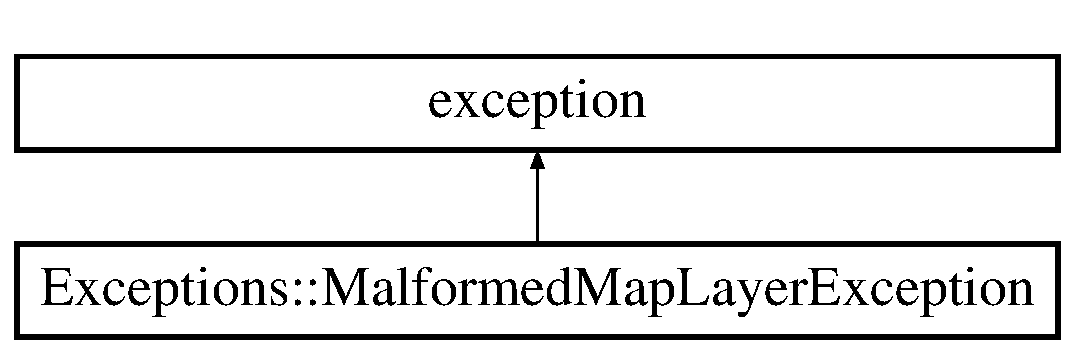
\includegraphics[height=2.000000cm]{class_exceptions_1_1_malformed_map_layer_exception}
\end{center}
\end{figure}
\subsection*{Public Member Functions}
\begin{DoxyCompactItemize}
\item 
\hyperlink{class_exceptions_1_1_malformed_map_layer_exception_a2c4ddb346485d08bbaea64b7b7753c32}{Malformed\+Map\+Layer\+Exception} ()
\item 
virtual const char $\ast$ \hyperlink{class_exceptions_1_1_malformed_map_layer_exception_a43cba83a23d960cc79ea3fa2c02fee6a}{what} () const   throw ()
\end{DoxyCompactItemize}


\subsection{Constructor \& Destructor Documentation}
\hypertarget{class_exceptions_1_1_malformed_map_layer_exception_a2c4ddb346485d08bbaea64b7b7753c32}{}\index{Exceptions\+::\+Malformed\+Map\+Layer\+Exception@{Exceptions\+::\+Malformed\+Map\+Layer\+Exception}!Malformed\+Map\+Layer\+Exception@{Malformed\+Map\+Layer\+Exception}}
\index{Malformed\+Map\+Layer\+Exception@{Malformed\+Map\+Layer\+Exception}!Exceptions\+::\+Malformed\+Map\+Layer\+Exception@{Exceptions\+::\+Malformed\+Map\+Layer\+Exception}}
\subsubsection[{Malformed\+Map\+Layer\+Exception}]{\setlength{\rightskip}{0pt plus 5cm}Exceptions\+::\+Malformed\+Map\+Layer\+Exception\+::\+Malformed\+Map\+Layer\+Exception (
\begin{DoxyParamCaption}
{}
\end{DoxyParamCaption}
)\hspace{0.3cm}{\ttfamily [inline]}}\label{class_exceptions_1_1_malformed_map_layer_exception_a2c4ddb346485d08bbaea64b7b7753c32}


\subsection{Member Function Documentation}
\hypertarget{class_exceptions_1_1_malformed_map_layer_exception_a43cba83a23d960cc79ea3fa2c02fee6a}{}\index{Exceptions\+::\+Malformed\+Map\+Layer\+Exception@{Exceptions\+::\+Malformed\+Map\+Layer\+Exception}!what@{what}}
\index{what@{what}!Exceptions\+::\+Malformed\+Map\+Layer\+Exception@{Exceptions\+::\+Malformed\+Map\+Layer\+Exception}}
\subsubsection[{what}]{\setlength{\rightskip}{0pt plus 5cm}virtual const char$\ast$ Exceptions\+::\+Malformed\+Map\+Layer\+Exception\+::what (
\begin{DoxyParamCaption}
{}
\end{DoxyParamCaption}
) const throw  ) \hspace{0.3cm}{\ttfamily [inline]}, {\ttfamily [virtual]}}\label{class_exceptions_1_1_malformed_map_layer_exception_a43cba83a23d960cc79ea3fa2c02fee6a}


The documentation for this class was generated from the following file\+:\begin{DoxyCompactItemize}
\item 
src/exceptions/\hyperlink{malformed__map__layer__exception_8h}{malformed\+\_\+map\+\_\+layer\+\_\+exception.\+h}\end{DoxyCompactItemize}

\hypertarget{struct_graphics_1_1_map_renderables}{}\section{Graphics\+:\+:Map\+Renderables Struct Reference}
\label{struct_graphics_1_1_map_renderables}\index{Graphics\+::\+Map\+Renderables@{Graphics\+::\+Map\+Renderables}}


{\ttfamily \#include $<$renderable\+\_\+factory.\+h$>$}

\subsection*{Public Attributes}
\begin{DoxyCompactItemize}
\item 
std\+::vector$<$ std\+::shared\+\_\+ptr$<$ \hyperlink{class_graphics_1_1_tile}{Tile} $>$ $>$ \hyperlink{struct_graphics_1_1_map_renderables_a6d34f842301b1673f8ec1b1637fa3972}{tiles}
\item 
std\+::vector$<$ \hyperlink{struct_graphics_1_1_animation_placeholder}{Animation\+Placeholder} $>$ \hyperlink{struct_graphics_1_1_map_renderables_a2cd42b457d91d533eb005154ade17687}{dynamic\+\_\+animations}
\end{DoxyCompactItemize}


\subsection{Member Data Documentation}
\hypertarget{struct_graphics_1_1_map_renderables_a2cd42b457d91d533eb005154ade17687}{}\index{Graphics\+::\+Map\+Renderables@{Graphics\+::\+Map\+Renderables}!dynamic\+\_\+animations@{dynamic\+\_\+animations}}
\index{dynamic\+\_\+animations@{dynamic\+\_\+animations}!Graphics\+::\+Map\+Renderables@{Graphics\+::\+Map\+Renderables}}
\subsubsection[{dynamic\+\_\+animations}]{\setlength{\rightskip}{0pt plus 5cm}std\+::vector$<${\bf Animation\+Placeholder}$>$ Graphics\+::\+Map\+Renderables\+::dynamic\+\_\+animations}\label{struct_graphics_1_1_map_renderables_a2cd42b457d91d533eb005154ade17687}
\hypertarget{struct_graphics_1_1_map_renderables_a6d34f842301b1673f8ec1b1637fa3972}{}\index{Graphics\+::\+Map\+Renderables@{Graphics\+::\+Map\+Renderables}!tiles@{tiles}}
\index{tiles@{tiles}!Graphics\+::\+Map\+Renderables@{Graphics\+::\+Map\+Renderables}}
\subsubsection[{tiles}]{\setlength{\rightskip}{0pt plus 5cm}std\+::vector$<$std\+::shared\+\_\+ptr$<${\bf Tile}$>$ $>$ Graphics\+::\+Map\+Renderables\+::tiles}\label{struct_graphics_1_1_map_renderables_a6d34f842301b1673f8ec1b1637fa3972}


The documentation for this struct was generated from the following file\+:\begin{DoxyCompactItemize}
\item 
src/graphics/\hyperlink{renderable__factory_8h}{renderable\+\_\+factory.\+h}\end{DoxyCompactItemize}

\hypertarget{class_input_1_1_mouse_button_event}{}\section{Input\+:\+:Mouse\+Button\+Event Class Reference}
\label{class_input_1_1_mouse_button_event}\index{Input\+::\+Mouse\+Button\+Event@{Input\+::\+Mouse\+Button\+Event}}


{\ttfamily \#include $<$mouse\+\_\+button\+\_\+event.\+h$>$}

Inheritance diagram for Input\+:\+:Mouse\+Button\+Event\+:\begin{figure}[H]
\begin{center}
\leavevmode
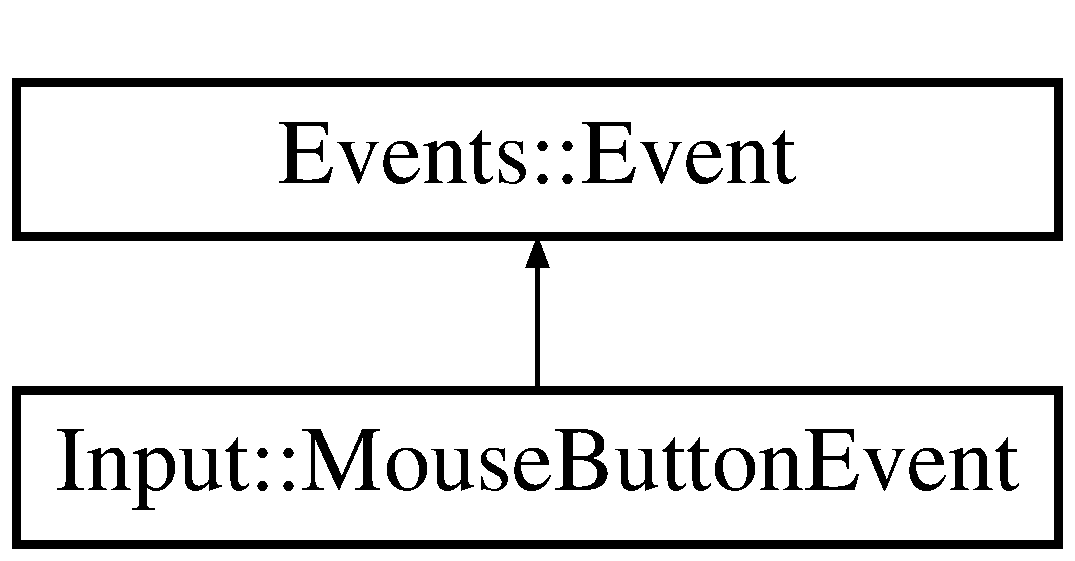
\includegraphics[height=2.000000cm]{class_input_1_1_mouse_button_event}
\end{center}
\end{figure}
\subsection*{Public Member Functions}
\begin{DoxyCompactItemize}
\item 
\hyperlink{class_input_1_1_mouse_button_event_ad53b26fb96fea26b8cc60e61c4298fd3}{Mouse\+Button\+Event} (const int \hyperlink{class_input_1_1_mouse_button_event_a94085b7e211bd8154dc4774b44786801}{button})
\item 
const int \hyperlink{class_input_1_1_mouse_button_event_a6723528770ad19668f97d2d4135d189e}{get\+Button} () const noexcept
\end{DoxyCompactItemize}
\subsection*{Private Attributes}
\begin{DoxyCompactItemize}
\item 
int \hyperlink{class_input_1_1_mouse_button_event_a94085b7e211bd8154dc4774b44786801}{button}
\end{DoxyCompactItemize}


\subsection{Constructor \& Destructor Documentation}
\hypertarget{class_input_1_1_mouse_button_event_ad53b26fb96fea26b8cc60e61c4298fd3}{}\index{Input\+::\+Mouse\+Button\+Event@{Input\+::\+Mouse\+Button\+Event}!Mouse\+Button\+Event@{Mouse\+Button\+Event}}
\index{Mouse\+Button\+Event@{Mouse\+Button\+Event}!Input\+::\+Mouse\+Button\+Event@{Input\+::\+Mouse\+Button\+Event}}
\subsubsection[{Mouse\+Button\+Event}]{\setlength{\rightskip}{0pt plus 5cm}Input\+::\+Mouse\+Button\+Event\+::\+Mouse\+Button\+Event (
\begin{DoxyParamCaption}
\item[{const int}]{button}
\end{DoxyParamCaption}
)\hspace{0.3cm}{\ttfamily [inline]}}\label{class_input_1_1_mouse_button_event_ad53b26fb96fea26b8cc60e61c4298fd3}


\subsection{Member Function Documentation}
\hypertarget{class_input_1_1_mouse_button_event_a6723528770ad19668f97d2d4135d189e}{}\index{Input\+::\+Mouse\+Button\+Event@{Input\+::\+Mouse\+Button\+Event}!get\+Button@{get\+Button}}
\index{get\+Button@{get\+Button}!Input\+::\+Mouse\+Button\+Event@{Input\+::\+Mouse\+Button\+Event}}
\subsubsection[{get\+Button}]{\setlength{\rightskip}{0pt plus 5cm}const int Input\+::\+Mouse\+Button\+Event\+::get\+Button (
\begin{DoxyParamCaption}
{}
\end{DoxyParamCaption}
) const\hspace{0.3cm}{\ttfamily [inline]}, {\ttfamily [noexcept]}}\label{class_input_1_1_mouse_button_event_a6723528770ad19668f97d2d4135d189e}


\subsection{Member Data Documentation}
\hypertarget{class_input_1_1_mouse_button_event_a94085b7e211bd8154dc4774b44786801}{}\index{Input\+::\+Mouse\+Button\+Event@{Input\+::\+Mouse\+Button\+Event}!button@{button}}
\index{button@{button}!Input\+::\+Mouse\+Button\+Event@{Input\+::\+Mouse\+Button\+Event}}
\subsubsection[{button}]{\setlength{\rightskip}{0pt plus 5cm}int Input\+::\+Mouse\+Button\+Event\+::button\hspace{0.3cm}{\ttfamily [private]}}\label{class_input_1_1_mouse_button_event_a94085b7e211bd8154dc4774b44786801}


The documentation for this class was generated from the following file\+:\begin{DoxyCompactItemize}
\item 
src/input/\hyperlink{mouse__button__event_8h}{mouse\+\_\+button\+\_\+event.\+h}\end{DoxyCompactItemize}

\hypertarget{class_input_1_1_mouse_cursor_event}{}\section{Input\+:\+:Mouse\+Cursor\+Event Class Reference}
\label{class_input_1_1_mouse_cursor_event}\index{Input\+::\+Mouse\+Cursor\+Event@{Input\+::\+Mouse\+Cursor\+Event}}


{\ttfamily \#include $<$mouse\+\_\+cursor\+\_\+event.\+h$>$}

Inheritance diagram for Input\+:\+:Mouse\+Cursor\+Event\+:\begin{figure}[H]
\begin{center}
\leavevmode
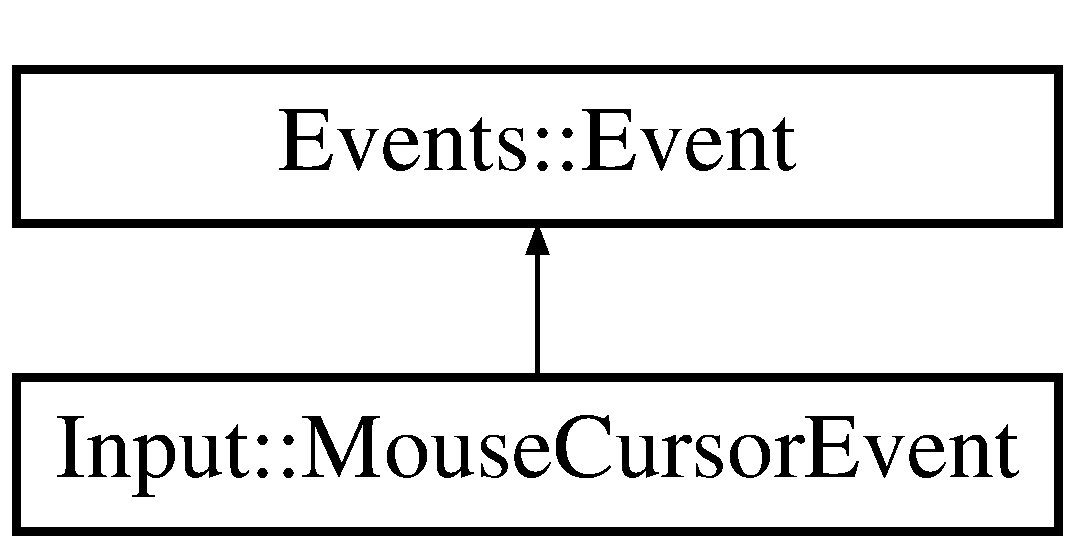
\includegraphics[height=2.000000cm]{class_input_1_1_mouse_cursor_event}
\end{center}
\end{figure}
\subsection*{Public Member Functions}
\begin{DoxyCompactItemize}
\item 
\hyperlink{class_input_1_1_mouse_cursor_event_afe151ce2560ff741558846c5a9a2699f}{Mouse\+Cursor\+Event} (const glm\+::dvec2 \&pos)
\item 
const glm\+::dvec2 \hyperlink{class_input_1_1_mouse_cursor_event_ac2fa10e773c505b02038da1fc7fe49ef}{get\+Position} () const noexcept
\end{DoxyCompactItemize}
\subsection*{Private Attributes}
\begin{DoxyCompactItemize}
\item 
glm\+::dvec2 \hyperlink{class_input_1_1_mouse_cursor_event_a8d62407dc243bc36660ea1c5e9970b65}{position}
\end{DoxyCompactItemize}


\subsection{Constructor \& Destructor Documentation}
\hypertarget{class_input_1_1_mouse_cursor_event_afe151ce2560ff741558846c5a9a2699f}{}\index{Input\+::\+Mouse\+Cursor\+Event@{Input\+::\+Mouse\+Cursor\+Event}!Mouse\+Cursor\+Event@{Mouse\+Cursor\+Event}}
\index{Mouse\+Cursor\+Event@{Mouse\+Cursor\+Event}!Input\+::\+Mouse\+Cursor\+Event@{Input\+::\+Mouse\+Cursor\+Event}}
\subsubsection[{Mouse\+Cursor\+Event}]{\setlength{\rightskip}{0pt plus 5cm}Input\+::\+Mouse\+Cursor\+Event\+::\+Mouse\+Cursor\+Event (
\begin{DoxyParamCaption}
\item[{const glm\+::dvec2 \&}]{pos}
\end{DoxyParamCaption}
)\hspace{0.3cm}{\ttfamily [inline]}}\label{class_input_1_1_mouse_cursor_event_afe151ce2560ff741558846c5a9a2699f}


\subsection{Member Function Documentation}
\hypertarget{class_input_1_1_mouse_cursor_event_ac2fa10e773c505b02038da1fc7fe49ef}{}\index{Input\+::\+Mouse\+Cursor\+Event@{Input\+::\+Mouse\+Cursor\+Event}!get\+Position@{get\+Position}}
\index{get\+Position@{get\+Position}!Input\+::\+Mouse\+Cursor\+Event@{Input\+::\+Mouse\+Cursor\+Event}}
\subsubsection[{get\+Position}]{\setlength{\rightskip}{0pt plus 5cm}const glm\+::dvec2 Input\+::\+Mouse\+Cursor\+Event\+::get\+Position (
\begin{DoxyParamCaption}
{}
\end{DoxyParamCaption}
) const\hspace{0.3cm}{\ttfamily [inline]}, {\ttfamily [noexcept]}}\label{class_input_1_1_mouse_cursor_event_ac2fa10e773c505b02038da1fc7fe49ef}


\subsection{Member Data Documentation}
\hypertarget{class_input_1_1_mouse_cursor_event_a8d62407dc243bc36660ea1c5e9970b65}{}\index{Input\+::\+Mouse\+Cursor\+Event@{Input\+::\+Mouse\+Cursor\+Event}!position@{position}}
\index{position@{position}!Input\+::\+Mouse\+Cursor\+Event@{Input\+::\+Mouse\+Cursor\+Event}}
\subsubsection[{position}]{\setlength{\rightskip}{0pt plus 5cm}glm\+::dvec2 Input\+::\+Mouse\+Cursor\+Event\+::position\hspace{0.3cm}{\ttfamily [private]}}\label{class_input_1_1_mouse_cursor_event_a8d62407dc243bc36660ea1c5e9970b65}


The documentation for this class was generated from the following file\+:\begin{DoxyCompactItemize}
\item 
src/input/\hyperlink{mouse__cursor__event_8h}{mouse\+\_\+cursor\+\_\+event.\+h}\end{DoxyCompactItemize}

\hypertarget{class_input_1_1_mouse_scroll_event}{}\section{Input\+:\+:Mouse\+Scroll\+Event Class Reference}
\label{class_input_1_1_mouse_scroll_event}\index{Input\+::\+Mouse\+Scroll\+Event@{Input\+::\+Mouse\+Scroll\+Event}}


{\ttfamily \#include $<$mouse\+\_\+scroll\+\_\+event.\+h$>$}

Inheritance diagram for Input\+:\+:Mouse\+Scroll\+Event\+:\begin{figure}[H]
\begin{center}
\leavevmode
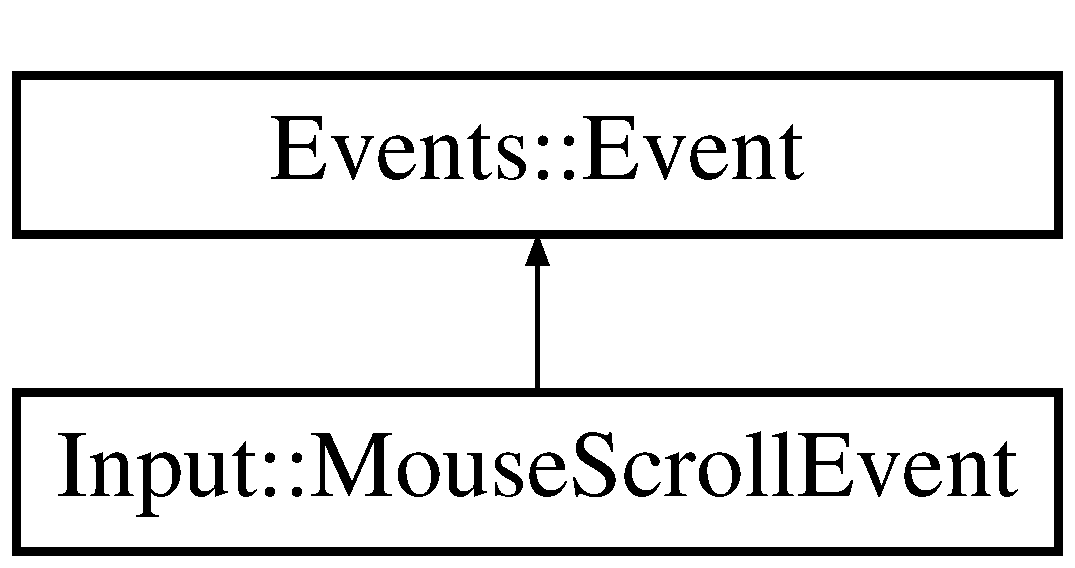
\includegraphics[height=2.000000cm]{class_input_1_1_mouse_scroll_event}
\end{center}
\end{figure}
\subsection*{Public Member Functions}
\begin{DoxyCompactItemize}
\item 
\hyperlink{class_input_1_1_mouse_scroll_event_aa5f6296ad33532b5a3c0bb57815415f7}{Mouse\+Scroll\+Event} (const glm\+::dvec2 \&\hyperlink{class_input_1_1_mouse_scroll_event_a6163719586771e6861bca6dd89476d4c}{offset})
\item 
const glm\+::dvec2 \hyperlink{class_input_1_1_mouse_scroll_event_a656e7f003aefd9ad5ebebc2093306de3}{get\+Position} () const noexcept
\end{DoxyCompactItemize}
\subsection*{Private Attributes}
\begin{DoxyCompactItemize}
\item 
glm\+::dvec2 \hyperlink{class_input_1_1_mouse_scroll_event_a6163719586771e6861bca6dd89476d4c}{offset}
\end{DoxyCompactItemize}


\subsection{Constructor \& Destructor Documentation}
\hypertarget{class_input_1_1_mouse_scroll_event_aa5f6296ad33532b5a3c0bb57815415f7}{}\index{Input\+::\+Mouse\+Scroll\+Event@{Input\+::\+Mouse\+Scroll\+Event}!Mouse\+Scroll\+Event@{Mouse\+Scroll\+Event}}
\index{Mouse\+Scroll\+Event@{Mouse\+Scroll\+Event}!Input\+::\+Mouse\+Scroll\+Event@{Input\+::\+Mouse\+Scroll\+Event}}
\subsubsection[{Mouse\+Scroll\+Event}]{\setlength{\rightskip}{0pt plus 5cm}Input\+::\+Mouse\+Scroll\+Event\+::\+Mouse\+Scroll\+Event (
\begin{DoxyParamCaption}
\item[{const glm\+::dvec2 \&}]{offset}
\end{DoxyParamCaption}
)\hspace{0.3cm}{\ttfamily [inline]}}\label{class_input_1_1_mouse_scroll_event_aa5f6296ad33532b5a3c0bb57815415f7}


\subsection{Member Function Documentation}
\hypertarget{class_input_1_1_mouse_scroll_event_a656e7f003aefd9ad5ebebc2093306de3}{}\index{Input\+::\+Mouse\+Scroll\+Event@{Input\+::\+Mouse\+Scroll\+Event}!get\+Position@{get\+Position}}
\index{get\+Position@{get\+Position}!Input\+::\+Mouse\+Scroll\+Event@{Input\+::\+Mouse\+Scroll\+Event}}
\subsubsection[{get\+Position}]{\setlength{\rightskip}{0pt plus 5cm}const glm\+::dvec2 Input\+::\+Mouse\+Scroll\+Event\+::get\+Position (
\begin{DoxyParamCaption}
{}
\end{DoxyParamCaption}
) const\hspace{0.3cm}{\ttfamily [inline]}, {\ttfamily [noexcept]}}\label{class_input_1_1_mouse_scroll_event_a656e7f003aefd9ad5ebebc2093306de3}


\subsection{Member Data Documentation}
\hypertarget{class_input_1_1_mouse_scroll_event_a6163719586771e6861bca6dd89476d4c}{}\index{Input\+::\+Mouse\+Scroll\+Event@{Input\+::\+Mouse\+Scroll\+Event}!offset@{offset}}
\index{offset@{offset}!Input\+::\+Mouse\+Scroll\+Event@{Input\+::\+Mouse\+Scroll\+Event}}
\subsubsection[{offset}]{\setlength{\rightskip}{0pt plus 5cm}glm\+::dvec2 Input\+::\+Mouse\+Scroll\+Event\+::offset\hspace{0.3cm}{\ttfamily [private]}}\label{class_input_1_1_mouse_scroll_event_a6163719586771e6861bca6dd89476d4c}


The documentation for this class was generated from the following file\+:\begin{DoxyCompactItemize}
\item 
src/input/\hyperlink{mouse__scroll__event_8h}{mouse\+\_\+scroll\+\_\+event.\+h}\end{DoxyCompactItemize}

\hypertarget{class_exceptions_1_1_no_camera_attached_exception}{}\section{Exceptions\+:\+:No\+Camera\+Attached\+Exception Class Reference}
\label{class_exceptions_1_1_no_camera_attached_exception}\index{Exceptions\+::\+No\+Camera\+Attached\+Exception@{Exceptions\+::\+No\+Camera\+Attached\+Exception}}


{\ttfamily \#include $<$no\+\_\+camera\+\_\+attached\+\_\+exception.\+h$>$}

Inheritance diagram for Exceptions\+:\+:No\+Camera\+Attached\+Exception\+:\begin{figure}[H]
\begin{center}
\leavevmode
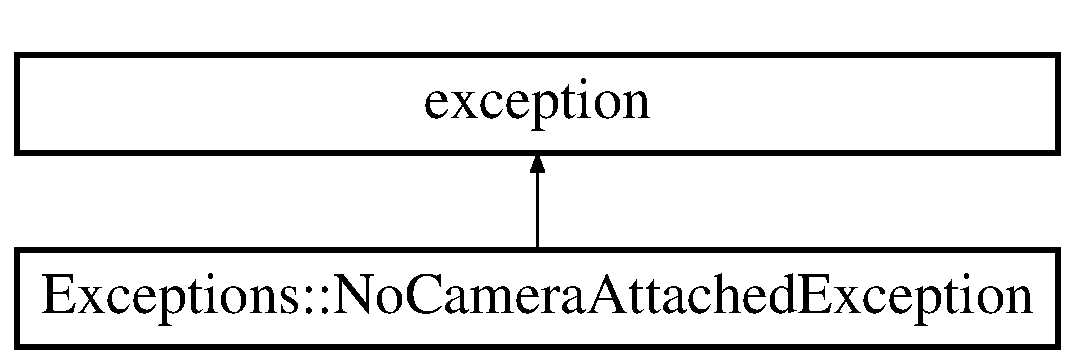
\includegraphics[height=2.000000cm]{class_exceptions_1_1_no_camera_attached_exception}
\end{center}
\end{figure}
\subsection*{Public Member Functions}
\begin{DoxyCompactItemize}
\item 
\hyperlink{class_exceptions_1_1_no_camera_attached_exception_a9208179f5460895247ac68769f628c89}{No\+Camera\+Attached\+Exception} ()
\item 
virtual const char $\ast$ \hyperlink{class_exceptions_1_1_no_camera_attached_exception_ad74e3adda749fb9d2affbab121b18c02}{what} () const   throw ()
\end{DoxyCompactItemize}


\subsection{Constructor \& Destructor Documentation}
\hypertarget{class_exceptions_1_1_no_camera_attached_exception_a9208179f5460895247ac68769f628c89}{}\index{Exceptions\+::\+No\+Camera\+Attached\+Exception@{Exceptions\+::\+No\+Camera\+Attached\+Exception}!No\+Camera\+Attached\+Exception@{No\+Camera\+Attached\+Exception}}
\index{No\+Camera\+Attached\+Exception@{No\+Camera\+Attached\+Exception}!Exceptions\+::\+No\+Camera\+Attached\+Exception@{Exceptions\+::\+No\+Camera\+Attached\+Exception}}
\subsubsection[{No\+Camera\+Attached\+Exception}]{\setlength{\rightskip}{0pt plus 5cm}Exceptions\+::\+No\+Camera\+Attached\+Exception\+::\+No\+Camera\+Attached\+Exception (
\begin{DoxyParamCaption}
{}
\end{DoxyParamCaption}
)\hspace{0.3cm}{\ttfamily [inline]}}\label{class_exceptions_1_1_no_camera_attached_exception_a9208179f5460895247ac68769f628c89}


\subsection{Member Function Documentation}
\hypertarget{class_exceptions_1_1_no_camera_attached_exception_ad74e3adda749fb9d2affbab121b18c02}{}\index{Exceptions\+::\+No\+Camera\+Attached\+Exception@{Exceptions\+::\+No\+Camera\+Attached\+Exception}!what@{what}}
\index{what@{what}!Exceptions\+::\+No\+Camera\+Attached\+Exception@{Exceptions\+::\+No\+Camera\+Attached\+Exception}}
\subsubsection[{what}]{\setlength{\rightskip}{0pt plus 5cm}virtual const char$\ast$ Exceptions\+::\+No\+Camera\+Attached\+Exception\+::what (
\begin{DoxyParamCaption}
{}
\end{DoxyParamCaption}
) const throw  ) \hspace{0.3cm}{\ttfamily [inline]}, {\ttfamily [virtual]}}\label{class_exceptions_1_1_no_camera_attached_exception_ad74e3adda749fb9d2affbab121b18c02}


The documentation for this class was generated from the following file\+:\begin{DoxyCompactItemize}
\item 
src/exceptions/\hyperlink{no__camera__attached__exception_8h}{no\+\_\+camera\+\_\+attached\+\_\+exception.\+h}\end{DoxyCompactItemize}

\hypertarget{class_events_1_1_observer}{}\section{Events\+:\+:Observer Class Reference}
\label{class_events_1_1_observer}\index{Events\+::\+Observer@{Events\+::\+Observer}}


{\ttfamily \#include $<$observer.\+h$>$}

Inheritance diagram for Events\+:\+:Observer\+:\begin{figure}[H]
\begin{center}
\leavevmode
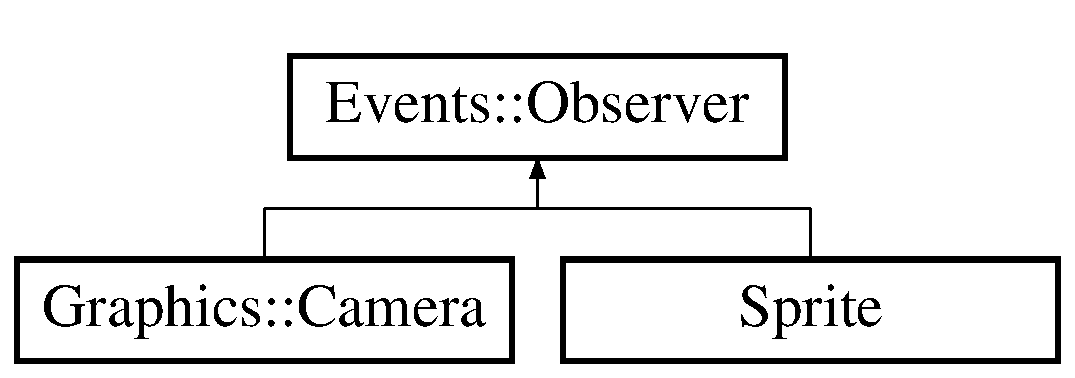
\includegraphics[height=2.000000cm]{class_events_1_1_observer}
\end{center}
\end{figure}
\subsection*{Public Member Functions}
\begin{DoxyCompactItemize}
\item 
virtual \hyperlink{class_events_1_1_observer_a5c867c0d95ecde7567f119385284c12d}{$\sim$\+Observer} ()
\item 
virtual void \hyperlink{class_events_1_1_observer_ad10e3ade9e803e9f706c5799da1d6525}{on\+Notify} (const \hyperlink{class_events_1_1_event}{Events\+::\+Event} \&event)=0
\end{DoxyCompactItemize}


\subsection{Constructor \& Destructor Documentation}
\hypertarget{class_events_1_1_observer_a5c867c0d95ecde7567f119385284c12d}{}\index{Events\+::\+Observer@{Events\+::\+Observer}!````~Observer@{$\sim$\+Observer}}
\index{````~Observer@{$\sim$\+Observer}!Events\+::\+Observer@{Events\+::\+Observer}}
\subsubsection[{$\sim$\+Observer}]{\setlength{\rightskip}{0pt plus 5cm}virtual Events\+::\+Observer\+::$\sim$\+Observer (
\begin{DoxyParamCaption}
{}
\end{DoxyParamCaption}
)\hspace{0.3cm}{\ttfamily [inline]}, {\ttfamily [virtual]}}\label{class_events_1_1_observer_a5c867c0d95ecde7567f119385284c12d}


\subsection{Member Function Documentation}
\hypertarget{class_events_1_1_observer_ad10e3ade9e803e9f706c5799da1d6525}{}\index{Events\+::\+Observer@{Events\+::\+Observer}!on\+Notify@{on\+Notify}}
\index{on\+Notify@{on\+Notify}!Events\+::\+Observer@{Events\+::\+Observer}}
\subsubsection[{on\+Notify}]{\setlength{\rightskip}{0pt plus 5cm}virtual void Events\+::\+Observer\+::on\+Notify (
\begin{DoxyParamCaption}
\item[{const {\bf Events\+::\+Event} \&}]{event}
\end{DoxyParamCaption}
)\hspace{0.3cm}{\ttfamily [pure virtual]}}\label{class_events_1_1_observer_ad10e3ade9e803e9f706c5799da1d6525}


Implemented in \hyperlink{class_graphics_1_1_camera_afd1785008e1ee71690749bf99a5d1e9a}{Graphics\+::\+Camera}, and \hyperlink{class_sprite_a86d7cca33da7b1e2681da6bd094be088}{Sprite}.



The documentation for this class was generated from the following file\+:\begin{DoxyCompactItemize}
\item 
src/events/\hyperlink{observer_8h}{observer.\+h}\end{DoxyCompactItemize}

\hypertarget{struct_graphics_1_1_graphics_system_1_1_ranked_light}{}\section{Graphics\+:\+:Graphics\+System\+:\+:Ranked\+Light Struct Reference}
\label{struct_graphics_1_1_graphics_system_1_1_ranked_light}\index{Graphics\+::\+Graphics\+System\+::\+Ranked\+Light@{Graphics\+::\+Graphics\+System\+::\+Ranked\+Light}}
\subsection*{Public Attributes}
\begin{DoxyCompactItemize}
\item 
std\+::shared\+\_\+ptr$<$ \hyperlink{class_graphics_1_1_light}{Light} $>$ \hyperlink{struct_graphics_1_1_graphics_system_1_1_ranked_light_a591a896fdc4a0cec0b9fe809e987587b}{light}
\item 
float \hyperlink{struct_graphics_1_1_graphics_system_1_1_ranked_light_ab649d7094a1c6a93dfa3f855d5b09820}{influence}
\end{DoxyCompactItemize}
\subsection*{Friends}
\begin{DoxyCompactItemize}
\item 
bool \hyperlink{struct_graphics_1_1_graphics_system_1_1_ranked_light_a4417f002ad1a700fa3ced08cb02e0e50}{operator$<$} (const \hyperlink{struct_graphics_1_1_graphics_system_1_1_ranked_light}{Ranked\+Light} \&left, const \hyperlink{struct_graphics_1_1_graphics_system_1_1_ranked_light}{Ranked\+Light} \&right)
\end{DoxyCompactItemize}


\subsection{Friends And Related Function Documentation}
\hypertarget{struct_graphics_1_1_graphics_system_1_1_ranked_light_a4417f002ad1a700fa3ced08cb02e0e50}{}\index{Graphics\+::\+Graphics\+System\+::\+Ranked\+Light@{Graphics\+::\+Graphics\+System\+::\+Ranked\+Light}!operator$<$@{operator$<$}}
\index{operator$<$@{operator$<$}!Graphics\+::\+Graphics\+System\+::\+Ranked\+Light@{Graphics\+::\+Graphics\+System\+::\+Ranked\+Light}}
\subsubsection[{operator$<$}]{\setlength{\rightskip}{0pt plus 5cm}bool operator$<$ (
\begin{DoxyParamCaption}
\item[{const {\bf Ranked\+Light} \&}]{left, }
\item[{const {\bf Ranked\+Light} \&}]{right}
\end{DoxyParamCaption}
)\hspace{0.3cm}{\ttfamily [friend]}}\label{struct_graphics_1_1_graphics_system_1_1_ranked_light_a4417f002ad1a700fa3ced08cb02e0e50}


\subsection{Member Data Documentation}
\hypertarget{struct_graphics_1_1_graphics_system_1_1_ranked_light_ab649d7094a1c6a93dfa3f855d5b09820}{}\index{Graphics\+::\+Graphics\+System\+::\+Ranked\+Light@{Graphics\+::\+Graphics\+System\+::\+Ranked\+Light}!influence@{influence}}
\index{influence@{influence}!Graphics\+::\+Graphics\+System\+::\+Ranked\+Light@{Graphics\+::\+Graphics\+System\+::\+Ranked\+Light}}
\subsubsection[{influence}]{\setlength{\rightskip}{0pt plus 5cm}float Graphics\+::\+Graphics\+System\+::\+Ranked\+Light\+::influence}\label{struct_graphics_1_1_graphics_system_1_1_ranked_light_ab649d7094a1c6a93dfa3f855d5b09820}
\hypertarget{struct_graphics_1_1_graphics_system_1_1_ranked_light_a591a896fdc4a0cec0b9fe809e987587b}{}\index{Graphics\+::\+Graphics\+System\+::\+Ranked\+Light@{Graphics\+::\+Graphics\+System\+::\+Ranked\+Light}!light@{light}}
\index{light@{light}!Graphics\+::\+Graphics\+System\+::\+Ranked\+Light@{Graphics\+::\+Graphics\+System\+::\+Ranked\+Light}}
\subsubsection[{light}]{\setlength{\rightskip}{0pt plus 5cm}std\+::shared\+\_\+ptr$<${\bf Light}$>$ Graphics\+::\+Graphics\+System\+::\+Ranked\+Light\+::light}\label{struct_graphics_1_1_graphics_system_1_1_ranked_light_a591a896fdc4a0cec0b9fe809e987587b}


The documentation for this struct was generated from the following file\+:\begin{DoxyCompactItemize}
\item 
src/graphics/\hyperlink{graphics__system_8h}{graphics\+\_\+system.\+h}\end{DoxyCompactItemize}

\hypertarget{class_graphics_1_1_renderable}{}\section{Graphics\+:\+:Renderable Class Reference}
\label{class_graphics_1_1_renderable}\index{Graphics\+::\+Renderable@{Graphics\+::\+Renderable}}


{\ttfamily \#include $<$renderable.\+h$>$}

Inheritance diagram for Graphics\+:\+:Renderable\+:\begin{figure}[H]
\begin{center}
\leavevmode
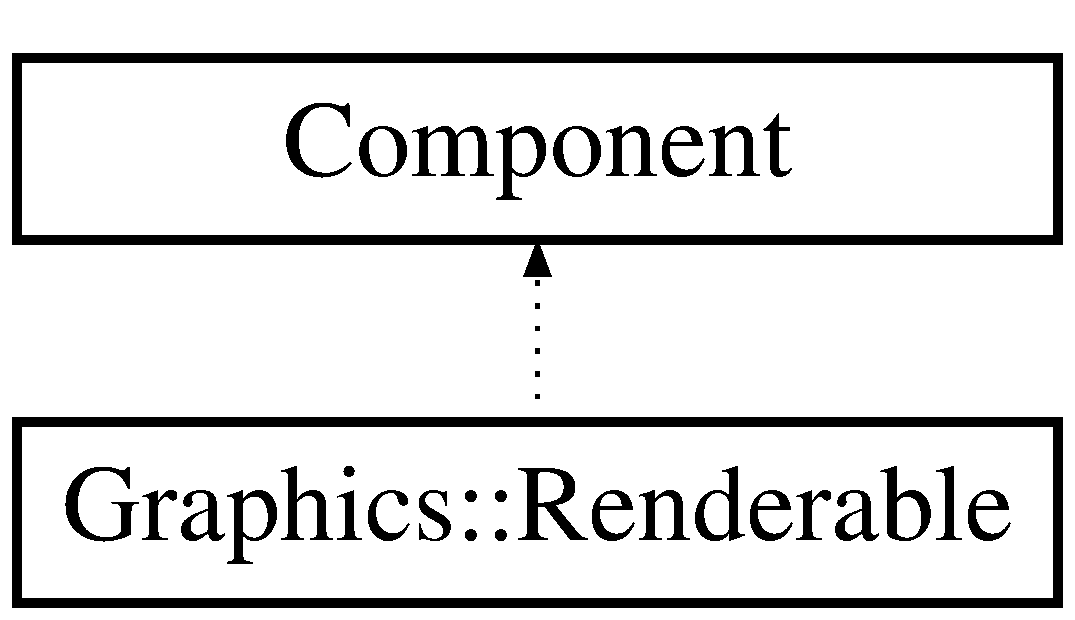
\includegraphics[height=4.000000cm]{class_graphics_1_1_renderable}
\end{center}
\end{figure}
\subsection*{Public Member Functions}
\begin{DoxyCompactItemize}
\item 
\hyperlink{class_graphics_1_1_renderable_a2c99d41631558194811f6f4c61a7f464}{Renderable} ()=delete
\item 
\hyperlink{class_graphics_1_1_renderable_a08ba323265fd34d219ed3495ee255c9b}{Renderable} (const unsigned int \hyperlink{class_graphics_1_1_renderable_aabfa91ebff7b10decd54119d663044ef}{vertex\+\_\+array\+\_\+object}, const \hyperlink{class_graphics_1_1_vertex_data}{Vertex\+Data} \&\hyperlink{class_graphics_1_1_renderable_a5077fe6a71021f0bd4ebc8d24cdf544b}{vertex\+\_\+data}, \hyperlink{class_graphics_1_1_base_attribute_trait}{Base\+Attribute\+Trait} $\ast$\hyperlink{class_graphics_1_1_renderable_a27f39fbb4866ccfc83f0662a59c03020}{trait}=new \hyperlink{class_graphics_1_1_renderable_attribute_trait}{Renderable\+Attribute\+Trait}())
\item 
\hyperlink{class_graphics_1_1_renderable_a7db48c39efa99650480cca6376bbf6c6}{Renderable} (const \hyperlink{class_graphics_1_1_renderable}{Renderable} \&)=delete
\item 
\hyperlink{class_graphics_1_1_renderable}{Renderable} \hyperlink{class_graphics_1_1_renderable_aa96e579c501d01462f5ee2ed5e949311}{operator=} (\hyperlink{class_graphics_1_1_renderable}{Renderable} \&)=delete
\item 
\hyperlink{class_graphics_1_1_renderable_a7edf9a0c89593ab500d5107e89f7bbae}{Renderable} (\hyperlink{class_graphics_1_1_renderable}{Renderable} \&\&renderable)
\item 
\hyperlink{class_graphics_1_1_renderable}{Renderable} \& \hyperlink{class_graphics_1_1_renderable_afac6ce4fffafffef11300fd13b763ef4}{operator=} (\hyperlink{class_graphics_1_1_renderable}{Renderable} \&\&renderable)
\item 
virtual \hyperlink{class_graphics_1_1_renderable_a63470b6e63ed9f87690569833fb48617}{$\sim$\+Renderable} ()
\item 
void \hyperlink{class_graphics_1_1_renderable_aab2e51991d63780654d7cc8a7083faca}{set\+Active} () noexcept
\item 
void \hyperlink{class_graphics_1_1_renderable_a9b6b9bf46beb9e4df9a0ba1dae55b87e}{set\+Inactive} () noexcept
\item 
const bool \hyperlink{class_graphics_1_1_renderable_a3ee6ae0274eaed19b731a97c5b44d2d6}{is\+Active} () const noexcept
\item 
void \hyperlink{class_graphics_1_1_renderable_a481dfc871e6129e8ee55482207ddc7fa}{set\+Shader} (std\+::shared\+\_\+ptr$<$ \hyperlink{class_graphics_1_1_shader}{Shader} $>$ shader\+\_\+object) noexcept
\item 
const std\+::shared\+\_\+ptr$<$ \hyperlink{class_graphics_1_1_shader}{Shader} $>$ \hyperlink{class_graphics_1_1_renderable_a542b918d1c6375ffdd06881d3fc31edd}{get\+Shader} () const noexcept
\item 
void \hyperlink{class_graphics_1_1_renderable_a8014f2c976291a09d452330448ca72d6}{add\+Texture} (std\+::shared\+\_\+ptr$<$ \hyperlink{class_graphics_1_1_base_texture}{Base\+Texture} $>$ texture\+\_\+object) noexcept
\item 
const std\+::vector$<$ std\+::shared\+\_\+ptr$<$ \hyperlink{class_graphics_1_1_base_texture}{Base\+Texture} $>$ $>$ \hyperlink{class_graphics_1_1_renderable_ac1634b94ac82b2b470010a3221c15643}{get\+Textures} () const noexcept
\item 
const std\+::shared\+\_\+ptr$<$ \hyperlink{class_graphics_1_1_base_texture}{Base\+Texture} $>$ \hyperlink{class_graphics_1_1_renderable_a9d134bc92527be7b68c65c8e5d70d8c0}{get\+Texture\+By\+Uniform} (const std\+::string \&uniform\+\_\+name)
\item 
void \hyperlink{class_graphics_1_1_renderable_a0166ebd26cac50f87ec7a33c5db9a3c5}{set\+Light\+Reactive} (const bool reactive) noexcept
\item 
const bool \hyperlink{class_graphics_1_1_renderable_a066fd1f919bdc7f2e562419f3e512dcd}{is\+Light\+Reactive} () const noexcept
\item 
void \hyperlink{class_graphics_1_1_renderable_ae50c65b85cb389df96b8e913b6dfe580}{set\+Ambient\+Light} (const glm\+::vec3 color) noexcept
\item 
const glm\+::vec3 \hyperlink{class_graphics_1_1_renderable_a9c000568c9df44433eceb76c5f1e39c0}{get\+Ambient\+Light} () const noexcept
\item 
void \hyperlink{class_graphics_1_1_renderable_acd1b9f38205aa1a637c46fe7faeed60c}{set\+Ambient\+Intensity} (const float intensity) noexcept
\item 
const float \hyperlink{class_graphics_1_1_renderable_a678da7336bb38a8cab7edf423f6dfed5}{get\+Ambient\+Intensity} () const noexcept
\item 
void \hyperlink{class_graphics_1_1_renderable_aa33e801d00279049d15e1a133f76eaf4}{add\+Influencing\+Light} (std\+::shared\+\_\+ptr$<$ \hyperlink{class_graphics_1_1_light}{Light} $>$ light) noexcept
\item 
void \hyperlink{class_graphics_1_1_renderable_a448be1ad2063cb3ff8b901a94ae0b566}{clear\+Influencing\+Lights} ()
\item 
const unsigned int \hyperlink{class_graphics_1_1_renderable_afde066c6e5ab15ce9b055f9f8f4593ff}{get\+Vertex\+Array\+Binding} () const noexcept
\item 
const \hyperlink{class_graphics_1_1_vertex_data}{Vertex\+Data} \hyperlink{class_graphics_1_1_renderable_a1d304b7063ae0acdef62b8041258a10b}{get\+Vertex\+Data} () const noexcept
\item 
virtual void \hyperlink{class_graphics_1_1_renderable_a6e20996de55215db7ffae2792aaaa88e}{on\+Destroy} () override
\item 
virtual void \hyperlink{class_graphics_1_1_renderable_a7433551970cd25e0241a4a5bb756ba50}{on\+Start} () override
\item 
virtual const bool \hyperlink{class_graphics_1_1_renderable_a7d0e820c55cb7f5c552aa0c1e846db76}{on\+Update} (const double delta) override
\begin{DoxyCompactList}\small\item\em \mbox{[}brief description\mbox{]} \end{DoxyCompactList}\item 
virtual const bool \hyperlink{class_graphics_1_1_renderable_afafd0e6147c73090234670934bbb8cbb}{on\+Render} ()
\end{DoxyCompactItemize}
\subsection*{Private Attributes}
\begin{DoxyCompactItemize}
\item 
bool \hyperlink{class_graphics_1_1_renderable_a5ee90a804fea73ddfaeed77086ecead4}{active}
\item 
unsigned int \hyperlink{class_graphics_1_1_renderable_aabfa91ebff7b10decd54119d663044ef}{vertex\+\_\+array\+\_\+object}
\item 
std\+::shared\+\_\+ptr$<$ \hyperlink{class_graphics_1_1_shader}{Shader} $>$ \hyperlink{class_graphics_1_1_renderable_a6c951dfc9a00d3f3f79550112d0f40e3}{shader}
\item 
std\+::vector$<$ std\+::shared\+\_\+ptr$<$ \hyperlink{class_graphics_1_1_base_texture}{Base\+Texture} $>$ $>$ \hyperlink{class_graphics_1_1_renderable_ac3a09a4fbb226022792d8abf07ff549a}{textures}
\item 
\hyperlink{class_graphics_1_1_vertex_data}{Vertex\+Data} \hyperlink{class_graphics_1_1_renderable_a5077fe6a71021f0bd4ebc8d24cdf544b}{vertex\+\_\+data}
\item 
std\+::unique\+\_\+ptr$<$ \hyperlink{class_graphics_1_1_base_attribute_trait}{Base\+Attribute\+Trait} $>$ \hyperlink{class_graphics_1_1_renderable_a27f39fbb4866ccfc83f0662a59c03020}{trait}
\item 
bool \hyperlink{class_graphics_1_1_renderable_a4a0fd8d55a1881c2b41e854ddb78366a}{light\+\_\+reactive}
\item 
std\+::list$<$ std\+::shared\+\_\+ptr$<$ \hyperlink{class_graphics_1_1_light}{Light} $>$ $>$ \hyperlink{class_graphics_1_1_renderable_a45bf29c03f8d47d870c6a1ce44126007}{influencing\+\_\+lights}
\item 
glm\+::vec3 \hyperlink{class_graphics_1_1_renderable_aecd9a143f7abb6c6b4969c147ee245c3}{ambient\+\_\+light}
\item 
float \hyperlink{class_graphics_1_1_renderable_a52fb337984cab44bb827037c9c13956e}{ambient\+\_\+intensity}
\end{DoxyCompactItemize}
\subsection*{Additional Inherited Members}


\subsection{Constructor \& Destructor Documentation}
\hypertarget{class_graphics_1_1_renderable_a2c99d41631558194811f6f4c61a7f464}{}\index{Graphics\+::\+Renderable@{Graphics\+::\+Renderable}!Renderable@{Renderable}}
\index{Renderable@{Renderable}!Graphics\+::\+Renderable@{Graphics\+::\+Renderable}}
\subsubsection[{Renderable}]{\setlength{\rightskip}{0pt plus 5cm}Graphics\+::\+Renderable\+::\+Renderable (
\begin{DoxyParamCaption}
{}
\end{DoxyParamCaption}
)\hspace{0.3cm}{\ttfamily [delete]}}\label{class_graphics_1_1_renderable_a2c99d41631558194811f6f4c61a7f464}
\hypertarget{class_graphics_1_1_renderable_a08ba323265fd34d219ed3495ee255c9b}{}\index{Graphics\+::\+Renderable@{Graphics\+::\+Renderable}!Renderable@{Renderable}}
\index{Renderable@{Renderable}!Graphics\+::\+Renderable@{Graphics\+::\+Renderable}}
\subsubsection[{Renderable}]{\setlength{\rightskip}{0pt plus 5cm}Graphics\+::\+Renderable\+::\+Renderable (
\begin{DoxyParamCaption}
\item[{const unsigned int}]{vertex\+\_\+array\+\_\+object, }
\item[{const {\bf Vertex\+Data} \&}]{vertex\+\_\+data, }
\item[{{\bf Base\+Attribute\+Trait} $\ast$}]{trait = {\ttfamily new~{\bf Renderable\+Attribute\+Trait}()}}
\end{DoxyParamCaption}
)}\label{class_graphics_1_1_renderable_a08ba323265fd34d219ed3495ee255c9b}
\hypertarget{class_graphics_1_1_renderable_a7db48c39efa99650480cca6376bbf6c6}{}\index{Graphics\+::\+Renderable@{Graphics\+::\+Renderable}!Renderable@{Renderable}}
\index{Renderable@{Renderable}!Graphics\+::\+Renderable@{Graphics\+::\+Renderable}}
\subsubsection[{Renderable}]{\setlength{\rightskip}{0pt plus 5cm}Graphics\+::\+Renderable\+::\+Renderable (
\begin{DoxyParamCaption}
\item[{const {\bf Renderable} \&}]{}
\end{DoxyParamCaption}
)\hspace{0.3cm}{\ttfamily [delete]}}\label{class_graphics_1_1_renderable_a7db48c39efa99650480cca6376bbf6c6}
\hypertarget{class_graphics_1_1_renderable_a7edf9a0c89593ab500d5107e89f7bbae}{}\index{Graphics\+::\+Renderable@{Graphics\+::\+Renderable}!Renderable@{Renderable}}
\index{Renderable@{Renderable}!Graphics\+::\+Renderable@{Graphics\+::\+Renderable}}
\subsubsection[{Renderable}]{\setlength{\rightskip}{0pt plus 5cm}Graphics\+::\+Renderable\+::\+Renderable (
\begin{DoxyParamCaption}
\item[{{\bf Renderable} \&\&}]{renderable}
\end{DoxyParamCaption}
)}\label{class_graphics_1_1_renderable_a7edf9a0c89593ab500d5107e89f7bbae}
\hypertarget{class_graphics_1_1_renderable_a63470b6e63ed9f87690569833fb48617}{}\index{Graphics\+::\+Renderable@{Graphics\+::\+Renderable}!````~Renderable@{$\sim$\+Renderable}}
\index{````~Renderable@{$\sim$\+Renderable}!Graphics\+::\+Renderable@{Graphics\+::\+Renderable}}
\subsubsection[{$\sim$\+Renderable}]{\setlength{\rightskip}{0pt plus 5cm}Graphics\+::\+Renderable\+::$\sim$\+Renderable (
\begin{DoxyParamCaption}
{}
\end{DoxyParamCaption}
)\hspace{0.3cm}{\ttfamily [virtual]}}\label{class_graphics_1_1_renderable_a63470b6e63ed9f87690569833fb48617}


\subsection{Member Function Documentation}
\hypertarget{class_graphics_1_1_renderable_aa33e801d00279049d15e1a133f76eaf4}{}\index{Graphics\+::\+Renderable@{Graphics\+::\+Renderable}!add\+Influencing\+Light@{add\+Influencing\+Light}}
\index{add\+Influencing\+Light@{add\+Influencing\+Light}!Graphics\+::\+Renderable@{Graphics\+::\+Renderable}}
\subsubsection[{add\+Influencing\+Light}]{\setlength{\rightskip}{0pt plus 5cm}void Graphics\+::\+Renderable\+::add\+Influencing\+Light (
\begin{DoxyParamCaption}
\item[{std\+::shared\+\_\+ptr$<$ {\bf Light} $>$}]{light}
\end{DoxyParamCaption}
)\hspace{0.3cm}{\ttfamily [noexcept]}}\label{class_graphics_1_1_renderable_aa33e801d00279049d15e1a133f76eaf4}
\hypertarget{class_graphics_1_1_renderable_a8014f2c976291a09d452330448ca72d6}{}\index{Graphics\+::\+Renderable@{Graphics\+::\+Renderable}!add\+Texture@{add\+Texture}}
\index{add\+Texture@{add\+Texture}!Graphics\+::\+Renderable@{Graphics\+::\+Renderable}}
\subsubsection[{add\+Texture}]{\setlength{\rightskip}{0pt plus 5cm}void Graphics\+::\+Renderable\+::add\+Texture (
\begin{DoxyParamCaption}
\item[{std\+::shared\+\_\+ptr$<$ {\bf Base\+Texture} $>$}]{texture\+\_\+object}
\end{DoxyParamCaption}
)\hspace{0.3cm}{\ttfamily [noexcept]}}\label{class_graphics_1_1_renderable_a8014f2c976291a09d452330448ca72d6}
\hypertarget{class_graphics_1_1_renderable_a448be1ad2063cb3ff8b901a94ae0b566}{}\index{Graphics\+::\+Renderable@{Graphics\+::\+Renderable}!clear\+Influencing\+Lights@{clear\+Influencing\+Lights}}
\index{clear\+Influencing\+Lights@{clear\+Influencing\+Lights}!Graphics\+::\+Renderable@{Graphics\+::\+Renderable}}
\subsubsection[{clear\+Influencing\+Lights}]{\setlength{\rightskip}{0pt plus 5cm}void Graphics\+::\+Renderable\+::clear\+Influencing\+Lights (
\begin{DoxyParamCaption}
{}
\end{DoxyParamCaption}
)}\label{class_graphics_1_1_renderable_a448be1ad2063cb3ff8b901a94ae0b566}
\hypertarget{class_graphics_1_1_renderable_a678da7336bb38a8cab7edf423f6dfed5}{}\index{Graphics\+::\+Renderable@{Graphics\+::\+Renderable}!get\+Ambient\+Intensity@{get\+Ambient\+Intensity}}
\index{get\+Ambient\+Intensity@{get\+Ambient\+Intensity}!Graphics\+::\+Renderable@{Graphics\+::\+Renderable}}
\subsubsection[{get\+Ambient\+Intensity}]{\setlength{\rightskip}{0pt plus 5cm}const float Graphics\+::\+Renderable\+::get\+Ambient\+Intensity (
\begin{DoxyParamCaption}
{}
\end{DoxyParamCaption}
) const\hspace{0.3cm}{\ttfamily [noexcept]}}\label{class_graphics_1_1_renderable_a678da7336bb38a8cab7edf423f6dfed5}
\hypertarget{class_graphics_1_1_renderable_a9c000568c9df44433eceb76c5f1e39c0}{}\index{Graphics\+::\+Renderable@{Graphics\+::\+Renderable}!get\+Ambient\+Light@{get\+Ambient\+Light}}
\index{get\+Ambient\+Light@{get\+Ambient\+Light}!Graphics\+::\+Renderable@{Graphics\+::\+Renderable}}
\subsubsection[{get\+Ambient\+Light}]{\setlength{\rightskip}{0pt plus 5cm}const glm\+::vec3 Graphics\+::\+Renderable\+::get\+Ambient\+Light (
\begin{DoxyParamCaption}
{}
\end{DoxyParamCaption}
) const\hspace{0.3cm}{\ttfamily [noexcept]}}\label{class_graphics_1_1_renderable_a9c000568c9df44433eceb76c5f1e39c0}
\hypertarget{class_graphics_1_1_renderable_a542b918d1c6375ffdd06881d3fc31edd}{}\index{Graphics\+::\+Renderable@{Graphics\+::\+Renderable}!get\+Shader@{get\+Shader}}
\index{get\+Shader@{get\+Shader}!Graphics\+::\+Renderable@{Graphics\+::\+Renderable}}
\subsubsection[{get\+Shader}]{\setlength{\rightskip}{0pt plus 5cm}const std\+::shared\+\_\+ptr$<$ {\bf Shader} $>$ Graphics\+::\+Renderable\+::get\+Shader (
\begin{DoxyParamCaption}
{}
\end{DoxyParamCaption}
) const\hspace{0.3cm}{\ttfamily [noexcept]}}\label{class_graphics_1_1_renderable_a542b918d1c6375ffdd06881d3fc31edd}
\hypertarget{class_graphics_1_1_renderable_a9d134bc92527be7b68c65c8e5d70d8c0}{}\index{Graphics\+::\+Renderable@{Graphics\+::\+Renderable}!get\+Texture\+By\+Uniform@{get\+Texture\+By\+Uniform}}
\index{get\+Texture\+By\+Uniform@{get\+Texture\+By\+Uniform}!Graphics\+::\+Renderable@{Graphics\+::\+Renderable}}
\subsubsection[{get\+Texture\+By\+Uniform}]{\setlength{\rightskip}{0pt plus 5cm}const std\+::shared\+\_\+ptr$<$ {\bf Base\+Texture} $>$ Graphics\+::\+Renderable\+::get\+Texture\+By\+Uniform (
\begin{DoxyParamCaption}
\item[{const std\+::string \&}]{uniform\+\_\+name}
\end{DoxyParamCaption}
)}\label{class_graphics_1_1_renderable_a9d134bc92527be7b68c65c8e5d70d8c0}
\hypertarget{class_graphics_1_1_renderable_ac1634b94ac82b2b470010a3221c15643}{}\index{Graphics\+::\+Renderable@{Graphics\+::\+Renderable}!get\+Textures@{get\+Textures}}
\index{get\+Textures@{get\+Textures}!Graphics\+::\+Renderable@{Graphics\+::\+Renderable}}
\subsubsection[{get\+Textures}]{\setlength{\rightskip}{0pt plus 5cm}const std\+::vector$<$ std\+::shared\+\_\+ptr$<$ {\bf Base\+Texture} $>$ $>$ Graphics\+::\+Renderable\+::get\+Textures (
\begin{DoxyParamCaption}
{}
\end{DoxyParamCaption}
) const\hspace{0.3cm}{\ttfamily [noexcept]}}\label{class_graphics_1_1_renderable_ac1634b94ac82b2b470010a3221c15643}
\hypertarget{class_graphics_1_1_renderable_afde066c6e5ab15ce9b055f9f8f4593ff}{}\index{Graphics\+::\+Renderable@{Graphics\+::\+Renderable}!get\+Vertex\+Array\+Binding@{get\+Vertex\+Array\+Binding}}
\index{get\+Vertex\+Array\+Binding@{get\+Vertex\+Array\+Binding}!Graphics\+::\+Renderable@{Graphics\+::\+Renderable}}
\subsubsection[{get\+Vertex\+Array\+Binding}]{\setlength{\rightskip}{0pt plus 5cm}const unsigned int Graphics\+::\+Renderable\+::get\+Vertex\+Array\+Binding (
\begin{DoxyParamCaption}
{}
\end{DoxyParamCaption}
) const\hspace{0.3cm}{\ttfamily [noexcept]}}\label{class_graphics_1_1_renderable_afde066c6e5ab15ce9b055f9f8f4593ff}
\hypertarget{class_graphics_1_1_renderable_a1d304b7063ae0acdef62b8041258a10b}{}\index{Graphics\+::\+Renderable@{Graphics\+::\+Renderable}!get\+Vertex\+Data@{get\+Vertex\+Data}}
\index{get\+Vertex\+Data@{get\+Vertex\+Data}!Graphics\+::\+Renderable@{Graphics\+::\+Renderable}}
\subsubsection[{get\+Vertex\+Data}]{\setlength{\rightskip}{0pt plus 5cm}const {\bf Vertex\+Data} Graphics\+::\+Renderable\+::get\+Vertex\+Data (
\begin{DoxyParamCaption}
{}
\end{DoxyParamCaption}
) const\hspace{0.3cm}{\ttfamily [noexcept]}}\label{class_graphics_1_1_renderable_a1d304b7063ae0acdef62b8041258a10b}
\hypertarget{class_graphics_1_1_renderable_a3ee6ae0274eaed19b731a97c5b44d2d6}{}\index{Graphics\+::\+Renderable@{Graphics\+::\+Renderable}!is\+Active@{is\+Active}}
\index{is\+Active@{is\+Active}!Graphics\+::\+Renderable@{Graphics\+::\+Renderable}}
\subsubsection[{is\+Active}]{\setlength{\rightskip}{0pt plus 5cm}const bool Graphics\+::\+Renderable\+::is\+Active (
\begin{DoxyParamCaption}
{}
\end{DoxyParamCaption}
) const\hspace{0.3cm}{\ttfamily [noexcept]}}\label{class_graphics_1_1_renderable_a3ee6ae0274eaed19b731a97c5b44d2d6}
\hypertarget{class_graphics_1_1_renderable_a066fd1f919bdc7f2e562419f3e512dcd}{}\index{Graphics\+::\+Renderable@{Graphics\+::\+Renderable}!is\+Light\+Reactive@{is\+Light\+Reactive}}
\index{is\+Light\+Reactive@{is\+Light\+Reactive}!Graphics\+::\+Renderable@{Graphics\+::\+Renderable}}
\subsubsection[{is\+Light\+Reactive}]{\setlength{\rightskip}{0pt plus 5cm}const bool Graphics\+::\+Renderable\+::is\+Light\+Reactive (
\begin{DoxyParamCaption}
{}
\end{DoxyParamCaption}
) const\hspace{0.3cm}{\ttfamily [noexcept]}}\label{class_graphics_1_1_renderable_a066fd1f919bdc7f2e562419f3e512dcd}
\hypertarget{class_graphics_1_1_renderable_a6e20996de55215db7ffae2792aaaa88e}{}\index{Graphics\+::\+Renderable@{Graphics\+::\+Renderable}!on\+Destroy@{on\+Destroy}}
\index{on\+Destroy@{on\+Destroy}!Graphics\+::\+Renderable@{Graphics\+::\+Renderable}}
\subsubsection[{on\+Destroy}]{\setlength{\rightskip}{0pt plus 5cm}void Graphics\+::\+Renderable\+::on\+Destroy (
\begin{DoxyParamCaption}
{}
\end{DoxyParamCaption}
)\hspace{0.3cm}{\ttfamily [override]}, {\ttfamily [virtual]}}\label{class_graphics_1_1_renderable_a6e20996de55215db7ffae2792aaaa88e}


Implements \hyperlink{class_component_a2b198f27162a6caf63917e304295f892}{Component}.



Reimplemented in \hyperlink{class_graphics_1_1_animated_tile_a9781b9b256a666a123fd2c050adb5118}{Graphics\+::\+Animated\+Tile}, and \hyperlink{class_graphics_1_1_tile_a28f5bdfa2fc61b292dda7ec15316b981}{Graphics\+::\+Tile}.

\hypertarget{class_graphics_1_1_renderable_afafd0e6147c73090234670934bbb8cbb}{}\index{Graphics\+::\+Renderable@{Graphics\+::\+Renderable}!on\+Render@{on\+Render}}
\index{on\+Render@{on\+Render}!Graphics\+::\+Renderable@{Graphics\+::\+Renderable}}
\subsubsection[{on\+Render}]{\setlength{\rightskip}{0pt plus 5cm}const bool Graphics\+::\+Renderable\+::on\+Render (
\begin{DoxyParamCaption}
{}
\end{DoxyParamCaption}
)\hspace{0.3cm}{\ttfamily [virtual]}}\label{class_graphics_1_1_renderable_afafd0e6147c73090234670934bbb8cbb}


Reimplemented in \hyperlink{class_graphics_1_1_animated_tile_a0b414dfdb18e4647652f8bb9334f9eee}{Graphics\+::\+Animated\+Tile}.

\hypertarget{class_graphics_1_1_renderable_a7433551970cd25e0241a4a5bb756ba50}{}\index{Graphics\+::\+Renderable@{Graphics\+::\+Renderable}!on\+Start@{on\+Start}}
\index{on\+Start@{on\+Start}!Graphics\+::\+Renderable@{Graphics\+::\+Renderable}}
\subsubsection[{on\+Start}]{\setlength{\rightskip}{0pt plus 5cm}void Graphics\+::\+Renderable\+::on\+Start (
\begin{DoxyParamCaption}
{}
\end{DoxyParamCaption}
)\hspace{0.3cm}{\ttfamily [override]}, {\ttfamily [virtual]}}\label{class_graphics_1_1_renderable_a7433551970cd25e0241a4a5bb756ba50}


Implements \hyperlink{class_component_a4a528a8790dbc141ffd0aba638b6dcc4}{Component}.



Reimplemented in \hyperlink{class_graphics_1_1_animated_tile_ad82e39321244cc2e06ee3df527473aba}{Graphics\+::\+Animated\+Tile}.

\hypertarget{class_graphics_1_1_renderable_a7d0e820c55cb7f5c552aa0c1e846db76}{}\index{Graphics\+::\+Renderable@{Graphics\+::\+Renderable}!on\+Update@{on\+Update}}
\index{on\+Update@{on\+Update}!Graphics\+::\+Renderable@{Graphics\+::\+Renderable}}
\subsubsection[{on\+Update}]{\setlength{\rightskip}{0pt plus 5cm}const bool Graphics\+::\+Renderable\+::on\+Update (
\begin{DoxyParamCaption}
\item[{const double}]{delta}
\end{DoxyParamCaption}
)\hspace{0.3cm}{\ttfamily [override]}, {\ttfamily [virtual]}}\label{class_graphics_1_1_renderable_a7d0e820c55cb7f5c552aa0c1e846db76}


\mbox{[}brief description\mbox{]} 

\mbox{[}long description\mbox{]} \begin{DoxyReturn}{Returns}
true if anything was updated, false if nothing was updated 
\end{DoxyReturn}


Implements \hyperlink{class_component_a8be284fccf4e97cee6705bd2d8f3705e}{Component}.



Reimplemented in \hyperlink{class_graphics_1_1_animated_tile_a2c6f7cd3866cad84b73ea5da8b92b76e}{Graphics\+::\+Animated\+Tile}, and \hyperlink{class_graphics_1_1_tile_a0311b1d9548f6badc9e81820b110cbb4}{Graphics\+::\+Tile}.

\hypertarget{class_graphics_1_1_renderable_aa96e579c501d01462f5ee2ed5e949311}{}\index{Graphics\+::\+Renderable@{Graphics\+::\+Renderable}!operator=@{operator=}}
\index{operator=@{operator=}!Graphics\+::\+Renderable@{Graphics\+::\+Renderable}}
\subsubsection[{operator=}]{\setlength{\rightskip}{0pt plus 5cm}{\bf Renderable} Graphics\+::\+Renderable\+::operator= (
\begin{DoxyParamCaption}
\item[{{\bf Renderable} \&}]{}
\end{DoxyParamCaption}
)\hspace{0.3cm}{\ttfamily [delete]}}\label{class_graphics_1_1_renderable_aa96e579c501d01462f5ee2ed5e949311}
\hypertarget{class_graphics_1_1_renderable_afac6ce4fffafffef11300fd13b763ef4}{}\index{Graphics\+::\+Renderable@{Graphics\+::\+Renderable}!operator=@{operator=}}
\index{operator=@{operator=}!Graphics\+::\+Renderable@{Graphics\+::\+Renderable}}
\subsubsection[{operator=}]{\setlength{\rightskip}{0pt plus 5cm}{\bf Renderable} \& Graphics\+::\+Renderable\+::operator= (
\begin{DoxyParamCaption}
\item[{{\bf Renderable} \&\&}]{renderable}
\end{DoxyParamCaption}
)}\label{class_graphics_1_1_renderable_afac6ce4fffafffef11300fd13b763ef4}
\hypertarget{class_graphics_1_1_renderable_aab2e51991d63780654d7cc8a7083faca}{}\index{Graphics\+::\+Renderable@{Graphics\+::\+Renderable}!set\+Active@{set\+Active}}
\index{set\+Active@{set\+Active}!Graphics\+::\+Renderable@{Graphics\+::\+Renderable}}
\subsubsection[{set\+Active}]{\setlength{\rightskip}{0pt plus 5cm}void Graphics\+::\+Renderable\+::set\+Active (
\begin{DoxyParamCaption}
{}
\end{DoxyParamCaption}
)\hspace{0.3cm}{\ttfamily [noexcept]}}\label{class_graphics_1_1_renderable_aab2e51991d63780654d7cc8a7083faca}
\hypertarget{class_graphics_1_1_renderable_acd1b9f38205aa1a637c46fe7faeed60c}{}\index{Graphics\+::\+Renderable@{Graphics\+::\+Renderable}!set\+Ambient\+Intensity@{set\+Ambient\+Intensity}}
\index{set\+Ambient\+Intensity@{set\+Ambient\+Intensity}!Graphics\+::\+Renderable@{Graphics\+::\+Renderable}}
\subsubsection[{set\+Ambient\+Intensity}]{\setlength{\rightskip}{0pt plus 5cm}void Graphics\+::\+Renderable\+::set\+Ambient\+Intensity (
\begin{DoxyParamCaption}
\item[{const float}]{intensity}
\end{DoxyParamCaption}
)\hspace{0.3cm}{\ttfamily [noexcept]}}\label{class_graphics_1_1_renderable_acd1b9f38205aa1a637c46fe7faeed60c}
\hypertarget{class_graphics_1_1_renderable_ae50c65b85cb389df96b8e913b6dfe580}{}\index{Graphics\+::\+Renderable@{Graphics\+::\+Renderable}!set\+Ambient\+Light@{set\+Ambient\+Light}}
\index{set\+Ambient\+Light@{set\+Ambient\+Light}!Graphics\+::\+Renderable@{Graphics\+::\+Renderable}}
\subsubsection[{set\+Ambient\+Light}]{\setlength{\rightskip}{0pt plus 5cm}void Graphics\+::\+Renderable\+::set\+Ambient\+Light (
\begin{DoxyParamCaption}
\item[{const glm\+::vec3}]{color}
\end{DoxyParamCaption}
)\hspace{0.3cm}{\ttfamily [noexcept]}}\label{class_graphics_1_1_renderable_ae50c65b85cb389df96b8e913b6dfe580}
\hypertarget{class_graphics_1_1_renderable_a9b6b9bf46beb9e4df9a0ba1dae55b87e}{}\index{Graphics\+::\+Renderable@{Graphics\+::\+Renderable}!set\+Inactive@{set\+Inactive}}
\index{set\+Inactive@{set\+Inactive}!Graphics\+::\+Renderable@{Graphics\+::\+Renderable}}
\subsubsection[{set\+Inactive}]{\setlength{\rightskip}{0pt plus 5cm}void Graphics\+::\+Renderable\+::set\+Inactive (
\begin{DoxyParamCaption}
{}
\end{DoxyParamCaption}
)\hspace{0.3cm}{\ttfamily [noexcept]}}\label{class_graphics_1_1_renderable_a9b6b9bf46beb9e4df9a0ba1dae55b87e}
\hypertarget{class_graphics_1_1_renderable_a0166ebd26cac50f87ec7a33c5db9a3c5}{}\index{Graphics\+::\+Renderable@{Graphics\+::\+Renderable}!set\+Light\+Reactive@{set\+Light\+Reactive}}
\index{set\+Light\+Reactive@{set\+Light\+Reactive}!Graphics\+::\+Renderable@{Graphics\+::\+Renderable}}
\subsubsection[{set\+Light\+Reactive}]{\setlength{\rightskip}{0pt plus 5cm}void Graphics\+::\+Renderable\+::set\+Light\+Reactive (
\begin{DoxyParamCaption}
\item[{const bool}]{reactive}
\end{DoxyParamCaption}
)\hspace{0.3cm}{\ttfamily [noexcept]}}\label{class_graphics_1_1_renderable_a0166ebd26cac50f87ec7a33c5db9a3c5}
\hypertarget{class_graphics_1_1_renderable_a481dfc871e6129e8ee55482207ddc7fa}{}\index{Graphics\+::\+Renderable@{Graphics\+::\+Renderable}!set\+Shader@{set\+Shader}}
\index{set\+Shader@{set\+Shader}!Graphics\+::\+Renderable@{Graphics\+::\+Renderable}}
\subsubsection[{set\+Shader}]{\setlength{\rightskip}{0pt plus 5cm}void Graphics\+::\+Renderable\+::set\+Shader (
\begin{DoxyParamCaption}
\item[{std\+::shared\+\_\+ptr$<$ {\bf Shader} $>$}]{shader\+\_\+object}
\end{DoxyParamCaption}
)\hspace{0.3cm}{\ttfamily [noexcept]}}\label{class_graphics_1_1_renderable_a481dfc871e6129e8ee55482207ddc7fa}


\subsection{Member Data Documentation}
\hypertarget{class_graphics_1_1_renderable_a5ee90a804fea73ddfaeed77086ecead4}{}\index{Graphics\+::\+Renderable@{Graphics\+::\+Renderable}!active@{active}}
\index{active@{active}!Graphics\+::\+Renderable@{Graphics\+::\+Renderable}}
\subsubsection[{active}]{\setlength{\rightskip}{0pt plus 5cm}bool Graphics\+::\+Renderable\+::active\hspace{0.3cm}{\ttfamily [private]}}\label{class_graphics_1_1_renderable_a5ee90a804fea73ddfaeed77086ecead4}
\hypertarget{class_graphics_1_1_renderable_a52fb337984cab44bb827037c9c13956e}{}\index{Graphics\+::\+Renderable@{Graphics\+::\+Renderable}!ambient\+\_\+intensity@{ambient\+\_\+intensity}}
\index{ambient\+\_\+intensity@{ambient\+\_\+intensity}!Graphics\+::\+Renderable@{Graphics\+::\+Renderable}}
\subsubsection[{ambient\+\_\+intensity}]{\setlength{\rightskip}{0pt plus 5cm}float Graphics\+::\+Renderable\+::ambient\+\_\+intensity\hspace{0.3cm}{\ttfamily [private]}}\label{class_graphics_1_1_renderable_a52fb337984cab44bb827037c9c13956e}
\hypertarget{class_graphics_1_1_renderable_aecd9a143f7abb6c6b4969c147ee245c3}{}\index{Graphics\+::\+Renderable@{Graphics\+::\+Renderable}!ambient\+\_\+light@{ambient\+\_\+light}}
\index{ambient\+\_\+light@{ambient\+\_\+light}!Graphics\+::\+Renderable@{Graphics\+::\+Renderable}}
\subsubsection[{ambient\+\_\+light}]{\setlength{\rightskip}{0pt plus 5cm}glm\+::vec3 Graphics\+::\+Renderable\+::ambient\+\_\+light\hspace{0.3cm}{\ttfamily [private]}}\label{class_graphics_1_1_renderable_aecd9a143f7abb6c6b4969c147ee245c3}
\hypertarget{class_graphics_1_1_renderable_a45bf29c03f8d47d870c6a1ce44126007}{}\index{Graphics\+::\+Renderable@{Graphics\+::\+Renderable}!influencing\+\_\+lights@{influencing\+\_\+lights}}
\index{influencing\+\_\+lights@{influencing\+\_\+lights}!Graphics\+::\+Renderable@{Graphics\+::\+Renderable}}
\subsubsection[{influencing\+\_\+lights}]{\setlength{\rightskip}{0pt plus 5cm}std\+::list$<$std\+::shared\+\_\+ptr$<${\bf Light}$>$ $>$ Graphics\+::\+Renderable\+::influencing\+\_\+lights\hspace{0.3cm}{\ttfamily [private]}}\label{class_graphics_1_1_renderable_a45bf29c03f8d47d870c6a1ce44126007}
\hypertarget{class_graphics_1_1_renderable_a4a0fd8d55a1881c2b41e854ddb78366a}{}\index{Graphics\+::\+Renderable@{Graphics\+::\+Renderable}!light\+\_\+reactive@{light\+\_\+reactive}}
\index{light\+\_\+reactive@{light\+\_\+reactive}!Graphics\+::\+Renderable@{Graphics\+::\+Renderable}}
\subsubsection[{light\+\_\+reactive}]{\setlength{\rightskip}{0pt plus 5cm}bool Graphics\+::\+Renderable\+::light\+\_\+reactive\hspace{0.3cm}{\ttfamily [private]}}\label{class_graphics_1_1_renderable_a4a0fd8d55a1881c2b41e854ddb78366a}
\hypertarget{class_graphics_1_1_renderable_a6c951dfc9a00d3f3f79550112d0f40e3}{}\index{Graphics\+::\+Renderable@{Graphics\+::\+Renderable}!shader@{shader}}
\index{shader@{shader}!Graphics\+::\+Renderable@{Graphics\+::\+Renderable}}
\subsubsection[{shader}]{\setlength{\rightskip}{0pt plus 5cm}std\+::shared\+\_\+ptr$<${\bf Shader}$>$ Graphics\+::\+Renderable\+::shader\hspace{0.3cm}{\ttfamily [private]}}\label{class_graphics_1_1_renderable_a6c951dfc9a00d3f3f79550112d0f40e3}
\hypertarget{class_graphics_1_1_renderable_ac3a09a4fbb226022792d8abf07ff549a}{}\index{Graphics\+::\+Renderable@{Graphics\+::\+Renderable}!textures@{textures}}
\index{textures@{textures}!Graphics\+::\+Renderable@{Graphics\+::\+Renderable}}
\subsubsection[{textures}]{\setlength{\rightskip}{0pt plus 5cm}std\+::vector$<$std\+::shared\+\_\+ptr$<${\bf Base\+Texture}$>$ $>$ Graphics\+::\+Renderable\+::textures\hspace{0.3cm}{\ttfamily [private]}}\label{class_graphics_1_1_renderable_ac3a09a4fbb226022792d8abf07ff549a}
\hypertarget{class_graphics_1_1_renderable_a27f39fbb4866ccfc83f0662a59c03020}{}\index{Graphics\+::\+Renderable@{Graphics\+::\+Renderable}!trait@{trait}}
\index{trait@{trait}!Graphics\+::\+Renderable@{Graphics\+::\+Renderable}}
\subsubsection[{trait}]{\setlength{\rightskip}{0pt plus 5cm}std\+::unique\+\_\+ptr$<${\bf Base\+Attribute\+Trait}$>$ Graphics\+::\+Renderable\+::trait\hspace{0.3cm}{\ttfamily [private]}}\label{class_graphics_1_1_renderable_a27f39fbb4866ccfc83f0662a59c03020}
\hypertarget{class_graphics_1_1_renderable_aabfa91ebff7b10decd54119d663044ef}{}\index{Graphics\+::\+Renderable@{Graphics\+::\+Renderable}!vertex\+\_\+array\+\_\+object@{vertex\+\_\+array\+\_\+object}}
\index{vertex\+\_\+array\+\_\+object@{vertex\+\_\+array\+\_\+object}!Graphics\+::\+Renderable@{Graphics\+::\+Renderable}}
\subsubsection[{vertex\+\_\+array\+\_\+object}]{\setlength{\rightskip}{0pt plus 5cm}unsigned int Graphics\+::\+Renderable\+::vertex\+\_\+array\+\_\+object\hspace{0.3cm}{\ttfamily [private]}}\label{class_graphics_1_1_renderable_aabfa91ebff7b10decd54119d663044ef}
\hypertarget{class_graphics_1_1_renderable_a5077fe6a71021f0bd4ebc8d24cdf544b}{}\index{Graphics\+::\+Renderable@{Graphics\+::\+Renderable}!vertex\+\_\+data@{vertex\+\_\+data}}
\index{vertex\+\_\+data@{vertex\+\_\+data}!Graphics\+::\+Renderable@{Graphics\+::\+Renderable}}
\subsubsection[{vertex\+\_\+data}]{\setlength{\rightskip}{0pt plus 5cm}{\bf Vertex\+Data} Graphics\+::\+Renderable\+::vertex\+\_\+data\hspace{0.3cm}{\ttfamily [private]}}\label{class_graphics_1_1_renderable_a5077fe6a71021f0bd4ebc8d24cdf544b}


The documentation for this class was generated from the following files\+:\begin{DoxyCompactItemize}
\item 
src/graphics/\hyperlink{renderable_8h}{renderable.\+h}\item 
src/graphics/\hyperlink{renderable_8cpp}{renderable.\+cpp}\end{DoxyCompactItemize}

\hypertarget{class_graphics_1_1_renderable_attribute_trait}{}\section{Graphics\+:\+:Renderable\+Attribute\+Trait Class Reference}
\label{class_graphics_1_1_renderable_attribute_trait}\index{Graphics\+::\+Renderable\+Attribute\+Trait@{Graphics\+::\+Renderable\+Attribute\+Trait}}


{\ttfamily \#include $<$renderable\+\_\+attribute\+\_\+trait.\+h$>$}

Inheritance diagram for Graphics\+:\+:Renderable\+Attribute\+Trait\+:\begin{figure}[H]
\begin{center}
\leavevmode
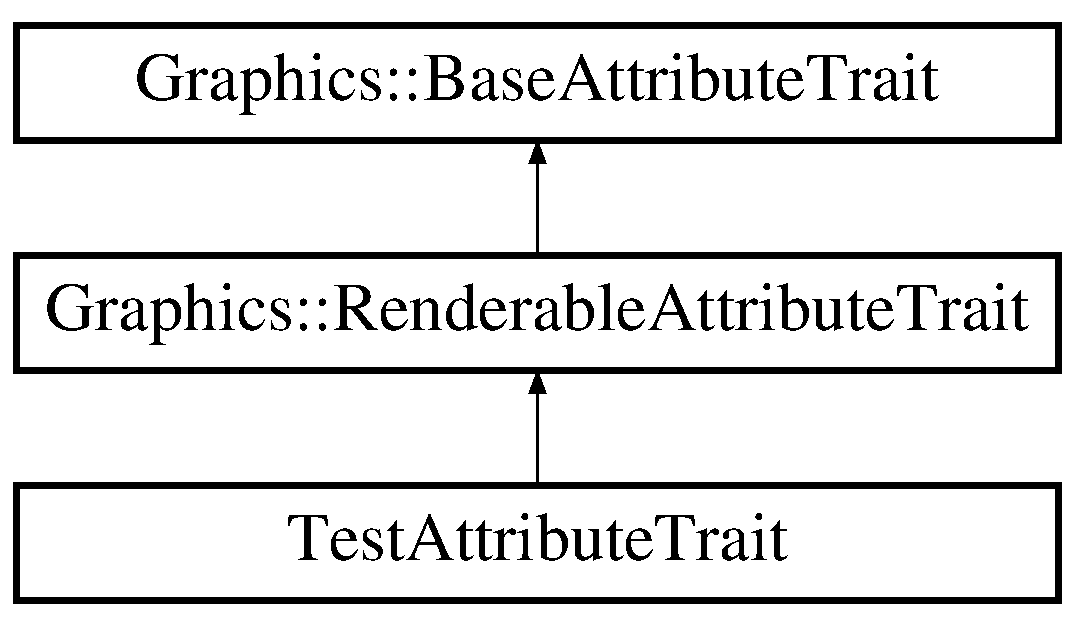
\includegraphics[height=3.000000cm]{class_graphics_1_1_renderable_attribute_trait}
\end{center}
\end{figure}
\subsection*{Public Member Functions}
\begin{DoxyCompactItemize}
\item 
\hyperlink{class_graphics_1_1_renderable_attribute_trait_afae7775a218a12c44a77c9d2190fccd3}{Renderable\+Attribute\+Trait} ()
\item 
virtual const std\+::map$<$ \hyperlink{class_graphics_1_1_vertex_data_a50e88236939dc2a3ec4df7aeb728620e}{Vertex\+Data\+::\+D\+A\+T\+A\+\_\+\+T\+Y\+P\+E}, unsigned int $>$ \hyperlink{class_graphics_1_1_renderable_attribute_trait_a44401f624ace1dc71220e7064db92465}{operator()} () const noexceptoverride
\end{DoxyCompactItemize}
\subsection*{Private Attributes}
\begin{DoxyCompactItemize}
\item 
std\+::map$<$ \hyperlink{class_graphics_1_1_vertex_data_a50e88236939dc2a3ec4df7aeb728620e}{Vertex\+Data\+::\+D\+A\+T\+A\+\_\+\+T\+Y\+P\+E}, unsigned int $>$ \hyperlink{class_graphics_1_1_renderable_attribute_trait_aa20fd62c99d1635eabe9a7fd73a67b32}{trait}
\end{DoxyCompactItemize}


\subsection{Constructor \& Destructor Documentation}
\hypertarget{class_graphics_1_1_renderable_attribute_trait_afae7775a218a12c44a77c9d2190fccd3}{}\index{Graphics\+::\+Renderable\+Attribute\+Trait@{Graphics\+::\+Renderable\+Attribute\+Trait}!Renderable\+Attribute\+Trait@{Renderable\+Attribute\+Trait}}
\index{Renderable\+Attribute\+Trait@{Renderable\+Attribute\+Trait}!Graphics\+::\+Renderable\+Attribute\+Trait@{Graphics\+::\+Renderable\+Attribute\+Trait}}
\subsubsection[{Renderable\+Attribute\+Trait}]{\setlength{\rightskip}{0pt plus 5cm}Graphics\+::\+Renderable\+Attribute\+Trait\+::\+Renderable\+Attribute\+Trait (
\begin{DoxyParamCaption}
{}
\end{DoxyParamCaption}
)\hspace{0.3cm}{\ttfamily [inline]}}\label{class_graphics_1_1_renderable_attribute_trait_afae7775a218a12c44a77c9d2190fccd3}


\subsection{Member Function Documentation}
\hypertarget{class_graphics_1_1_renderable_attribute_trait_a44401f624ace1dc71220e7064db92465}{}\index{Graphics\+::\+Renderable\+Attribute\+Trait@{Graphics\+::\+Renderable\+Attribute\+Trait}!operator()@{operator()}}
\index{operator()@{operator()}!Graphics\+::\+Renderable\+Attribute\+Trait@{Graphics\+::\+Renderable\+Attribute\+Trait}}
\subsubsection[{operator()}]{\setlength{\rightskip}{0pt plus 5cm}virtual const std\+::map$<${\bf Vertex\+Data\+::\+D\+A\+T\+A\+\_\+\+T\+Y\+P\+E}, unsigned int$>$ Graphics\+::\+Renderable\+Attribute\+Trait\+::operator() (
\begin{DoxyParamCaption}
{}
\end{DoxyParamCaption}
) const\hspace{0.3cm}{\ttfamily [inline]}, {\ttfamily [override]}, {\ttfamily [virtual]}, {\ttfamily [noexcept]}}\label{class_graphics_1_1_renderable_attribute_trait_a44401f624ace1dc71220e7064db92465}


Implements \hyperlink{class_graphics_1_1_base_attribute_trait_a7f43cabd619b64be1a0056e0fe568cf5}{Graphics\+::\+Base\+Attribute\+Trait}.



Reimplemented in \hyperlink{class_test_attribute_trait_af121ef5fbd5bcda4bbbc7fdadd5599c8}{Test\+Attribute\+Trait}.



\subsection{Member Data Documentation}
\hypertarget{class_graphics_1_1_renderable_attribute_trait_aa20fd62c99d1635eabe9a7fd73a67b32}{}\index{Graphics\+::\+Renderable\+Attribute\+Trait@{Graphics\+::\+Renderable\+Attribute\+Trait}!trait@{trait}}
\index{trait@{trait}!Graphics\+::\+Renderable\+Attribute\+Trait@{Graphics\+::\+Renderable\+Attribute\+Trait}}
\subsubsection[{trait}]{\setlength{\rightskip}{0pt plus 5cm}std\+::map$<${\bf Vertex\+Data\+::\+D\+A\+T\+A\+\_\+\+T\+Y\+P\+E}, unsigned int$>$ Graphics\+::\+Renderable\+Attribute\+Trait\+::trait\hspace{0.3cm}{\ttfamily [private]}}\label{class_graphics_1_1_renderable_attribute_trait_aa20fd62c99d1635eabe9a7fd73a67b32}


The documentation for this class was generated from the following file\+:\begin{DoxyCompactItemize}
\item 
src/graphics/\hyperlink{renderable__attribute__trait_8h}{renderable\+\_\+attribute\+\_\+trait.\+h}\end{DoxyCompactItemize}

\hypertarget{class_graphics_1_1_renderable_factory}{}\section{Graphics\+:\+:Renderable\+Factory Class Reference}
\label{class_graphics_1_1_renderable_factory}\index{Graphics\+::\+Renderable\+Factory@{Graphics\+::\+Renderable\+Factory}}


{\ttfamily \#include $<$renderable\+\_\+factory.\+h$>$}

\subsection*{Classes}
\begin{DoxyCompactItemize}
\item 
struct \hyperlink{struct_graphics_1_1_renderable_factory_1_1_renderable_info}{Renderable\+Info}
\end{DoxyCompactItemize}
\subsection*{Public Member Functions}
\begin{DoxyCompactItemize}
\item 
\hyperlink{class_graphics_1_1_renderable_factory_aa48147a2a3e11c1a03d1aed7b4b3889b}{Renderable\+Factory} ()
\item 
\hyperlink{class_graphics_1_1_renderable_factory_aed9ccae586d31d05b6c6a09a7bb37b44}{$\sim$\+Renderable\+Factory} ()
\item 
{\footnotesize template$<$class T $>$ }\\std\+::shared\+\_\+ptr$<$ T $>$ \hyperlink{class_graphics_1_1_renderable_factory_a732457c06858debc4870d7a77568d0dd}{create} ()
\item 
{\footnotesize template$<$class T $>$ }\\std\+::shared\+\_\+ptr$<$ T $>$ \hyperlink{class_graphics_1_1_renderable_factory_abaf13a568934efa1a785ed38622bcbbe}{create} (const \hyperlink{class_graphics_1_1_vertex_data}{Vertex\+Data} \&vertex\+\_\+data)
\item 
std\+::vector$<$ std\+::shared\+\_\+ptr$<$ \hyperlink{class_graphics_1_1_light}{Light} $>$ $>$ \hyperlink{class_graphics_1_1_renderable_factory_af1b3f07c26ee6aed903f3611a93a284d}{create\+Lights\+From\+Map} (const Tmx\+::\+Map \&map)
\item 
\hyperlink{struct_graphics_1_1_map_renderables}{Map\+Renderables} \hyperlink{class_graphics_1_1_renderable_factory_a06a17225aeaa74b05c6595e02c66c8d3}{create\+From\+Map} (const Tmx\+::\+Map \&map, \hyperlink{class_graphics_1_1_texture_manager}{Texture\+Manager} \&texture\+\_\+manager, const std\+::shared\+\_\+ptr$<$ \hyperlink{class_graphics_1_1_shader_manager}{Shader\+Manager} $>$ shader\+\_\+manager)
\item 
std\+::vector$<$ std\+::shared\+\_\+ptr$<$ \hyperlink{class_graphics_1_1_animated_tile}{Animated\+Tile} $>$ $>$ \hyperlink{class_graphics_1_1_renderable_factory_ab2c5c37f969c72c2554a9b19b7fe5a7a}{create\+Statically\+Animated\+Tiles\+From\+Map} (const Tmx\+::\+Map \&map, \hyperlink{class_graphics_1_1_texture_manager}{Texture\+Manager} \&texture\+\_\+manager, const std\+::shared\+\_\+ptr$<$ \hyperlink{class_graphics_1_1_shader_manager}{Shader\+Manager} $>$ shader\+\_\+manager)
\item 
std\+::vector$<$ \hyperlink{struct_graphics_1_1_animation}{Animation} $>$ \hyperlink{class_graphics_1_1_renderable_factory_a8143ae8f07bc174cab9da6f8b2250d3c}{create\+Animations\+From\+Animation\+Map} (const Tmx\+::\+Map \&map, \hyperlink{class_graphics_1_1_texture_manager}{Texture\+Manager} \&texture\+\_\+manager, const std\+::shared\+\_\+ptr$<$ \hyperlink{class_graphics_1_1_shader_manager}{Shader\+Manager} $>$ shader\+\_\+manager)
\item 
{\footnotesize template$<$$>$ }\\std\+::shared\+\_\+ptr$<$ \hyperlink{class_graphics_1_1_renderable}{Renderable} $>$ \hyperlink{class_graphics_1_1_renderable_factory_a589bdf269f560834104518482cb7f49c}{create} ()
\item 
{\footnotesize template$<$$>$ }\\std\+::shared\+\_\+ptr$<$ \hyperlink{class_graphics_1_1_tile}{Tile} $>$ \hyperlink{class_graphics_1_1_renderable_factory_a38c0da2947f41201d69fbde65430d859}{create} ()
\item 
{\footnotesize template$<$$>$ }\\std\+::shared\+\_\+ptr$<$ \hyperlink{class_graphics_1_1_animated_tile}{Animated\+Tile} $>$ \hyperlink{class_graphics_1_1_renderable_factory_a618735c8b4ee8ca099974211bac5c2ad}{create} ()
\item 
{\footnotesize template$<$$>$ }\\std\+::shared\+\_\+ptr$<$ \hyperlink{class_graphics_1_1_renderable}{Renderable} $>$ \hyperlink{class_graphics_1_1_renderable_factory_a5e3db739ae2aa08a42aeff57c3270554}{create} (const \hyperlink{class_graphics_1_1_vertex_data}{Vertex\+Data} \&vertex\+\_\+data)
\item 
{\footnotesize template$<$$>$ }\\std\+::shared\+\_\+ptr$<$ \hyperlink{class_graphics_1_1_tile}{Tile} $>$ \hyperlink{class_graphics_1_1_renderable_factory_ada89b5ddcb66665e89c64837d2e3f0a0}{create} (const \hyperlink{class_graphics_1_1_vertex_data}{Vertex\+Data} \&vertex\+\_\+data)
\item 
{\footnotesize template$<$$>$ }\\std\+::shared\+\_\+ptr$<$ \hyperlink{class_graphics_1_1_animated_tile}{Animated\+Tile} $>$ \hyperlink{class_graphics_1_1_renderable_factory_aa01ea09b848a60069b32135e75ff2fda}{create} (const \hyperlink{class_graphics_1_1_vertex_data}{Vertex\+Data} \&vertex\+\_\+data)
\end{DoxyCompactItemize}
\subsection*{Private Member Functions}
\begin{DoxyCompactItemize}
\item 
const \hyperlink{class_graphics_1_1_vertex_data}{Vertex\+Data} \hyperlink{class_graphics_1_1_renderable_factory_a0688e8bccb6104c68101e14ab39c258e}{generate\+Cube} ()
\item 
const \hyperlink{class_graphics_1_1_vertex_data}{Vertex\+Data} \hyperlink{class_graphics_1_1_renderable_factory_afbf0b634230088f4301505ff49162955}{generate\+Tile} (const unsigned int base\+\_\+size, const unsigned int current\+\_\+size)
\item 
unsigned int \hyperlink{class_graphics_1_1_renderable_factory_a51abec6e45fe118195fbd71530995173}{generate\+Vertex\+Array\+Object} (\hyperlink{class_graphics_1_1_vertex_data}{Vertex\+Data} vertex\+\_\+data)
\item 
std\+::shared\+\_\+ptr$<$ \hyperlink{class_graphics_1_1_base_texture}{Base\+Texture} $>$ \hyperlink{class_graphics_1_1_renderable_factory_a9810a7f53bc6c5823f9183b19413e593}{texture\+From\+Tileset} (const Tmx\+::\+Tileset $\ast$tileset, \hyperlink{class_graphics_1_1_texture_manager}{Texture\+Manager} \&texture\+\_\+manager, const std\+::string \&path, const std\+::string \&uniform\+\_\+name)
\item 
std\+::shared\+\_\+ptr$<$ \hyperlink{class_graphics_1_1_base_texture}{Base\+Texture} $>$ \hyperlink{class_graphics_1_1_renderable_factory_aba39fff9384bb9fabda4c633c71a8ce4}{normal\+Texture\+From\+Tileset} (const Tmx\+::\+Tileset $\ast$tileset, \hyperlink{class_graphics_1_1_texture_manager}{Texture\+Manager} \&texture\+\_\+manager, const std\+::string \&path, const std\+::string \&uniform\+\_\+name)
\item 
std\+::shared\+\_\+ptr$<$ \hyperlink{class_graphics_1_1_base_texture}{Base\+Texture} $>$ \hyperlink{class_graphics_1_1_renderable_factory_aab9ffc72af0ad3d403daabb746865a52}{displacement\+Texture\+From\+Tileset} (const Tmx\+::\+Tileset $\ast$tileset, \hyperlink{class_graphics_1_1_texture_manager}{Texture\+Manager} \&texture\+\_\+manager, const std\+::string \&path, const std\+::string \&uniform\+\_\+name)
\item 
std\+::vector$<$ glm\+::vec2 $>$ \hyperlink{class_graphics_1_1_renderable_factory_ae9ca8626793c8830412112679fb40726}{generate\+Texture\+Coords} (const Tmx\+::\+Tile\+Layer $\ast$layer, const unsigned int x\+\_\+pos, const unsigned int y\+\_\+pos, const unsigned int texture\+\_\+width, const unsigned int texture\+\_\+height, const unsigned int tile\+\_\+width, const unsigned int tile\+\_\+height)
\item 
std\+::vector$<$ glm\+::vec3 $>$ \hyperlink{class_graphics_1_1_renderable_factory_aec007081a7fa5ab143461adecd13ca33}{generate\+Vertex\+Coords} (const unsigned int base\+\_\+size, const unsigned int current\+\_\+size)
\end{DoxyCompactItemize}
\subsection*{Private Attributes}
\begin{DoxyCompactItemize}
\item 
unsigned int \hyperlink{class_graphics_1_1_renderable_factory_ada5e3359529345b7c9d0498f54eab5a4}{animated\+\_\+tile\+\_\+vao}
\end{DoxyCompactItemize}


\subsection{Constructor \& Destructor Documentation}
\hypertarget{class_graphics_1_1_renderable_factory_aa48147a2a3e11c1a03d1aed7b4b3889b}{}\index{Graphics\+::\+Renderable\+Factory@{Graphics\+::\+Renderable\+Factory}!Renderable\+Factory@{Renderable\+Factory}}
\index{Renderable\+Factory@{Renderable\+Factory}!Graphics\+::\+Renderable\+Factory@{Graphics\+::\+Renderable\+Factory}}
\subsubsection[{Renderable\+Factory}]{\setlength{\rightskip}{0pt plus 5cm}Graphics\+::\+Renderable\+Factory\+::\+Renderable\+Factory (
\begin{DoxyParamCaption}
{}
\end{DoxyParamCaption}
)}\label{class_graphics_1_1_renderable_factory_aa48147a2a3e11c1a03d1aed7b4b3889b}
\hypertarget{class_graphics_1_1_renderable_factory_aed9ccae586d31d05b6c6a09a7bb37b44}{}\index{Graphics\+::\+Renderable\+Factory@{Graphics\+::\+Renderable\+Factory}!````~Renderable\+Factory@{$\sim$\+Renderable\+Factory}}
\index{````~Renderable\+Factory@{$\sim$\+Renderable\+Factory}!Graphics\+::\+Renderable\+Factory@{Graphics\+::\+Renderable\+Factory}}
\subsubsection[{$\sim$\+Renderable\+Factory}]{\setlength{\rightskip}{0pt plus 5cm}Graphics\+::\+Renderable\+Factory\+::$\sim$\+Renderable\+Factory (
\begin{DoxyParamCaption}
{}
\end{DoxyParamCaption}
)}\label{class_graphics_1_1_renderable_factory_aed9ccae586d31d05b6c6a09a7bb37b44}


\subsection{Member Function Documentation}
\hypertarget{class_graphics_1_1_renderable_factory_a732457c06858debc4870d7a77568d0dd}{}\index{Graphics\+::\+Renderable\+Factory@{Graphics\+::\+Renderable\+Factory}!create@{create}}
\index{create@{create}!Graphics\+::\+Renderable\+Factory@{Graphics\+::\+Renderable\+Factory}}
\subsubsection[{create}]{\setlength{\rightskip}{0pt plus 5cm}template$<$class T $>$ std\+::shared\+\_\+ptr$<$T$>$ Graphics\+::\+Renderable\+Factory\+::create (
\begin{DoxyParamCaption}
{}
\end{DoxyParamCaption}
)}\label{class_graphics_1_1_renderable_factory_a732457c06858debc4870d7a77568d0dd}
\hypertarget{class_graphics_1_1_renderable_factory_abaf13a568934efa1a785ed38622bcbbe}{}\index{Graphics\+::\+Renderable\+Factory@{Graphics\+::\+Renderable\+Factory}!create@{create}}
\index{create@{create}!Graphics\+::\+Renderable\+Factory@{Graphics\+::\+Renderable\+Factory}}
\subsubsection[{create}]{\setlength{\rightskip}{0pt plus 5cm}template$<$class T $>$ std\+::shared\+\_\+ptr$<$T$>$ Graphics\+::\+Renderable\+Factory\+::create (
\begin{DoxyParamCaption}
\item[{const {\bf Vertex\+Data} \&}]{vertex\+\_\+data}
\end{DoxyParamCaption}
)}\label{class_graphics_1_1_renderable_factory_abaf13a568934efa1a785ed38622bcbbe}
\hypertarget{class_graphics_1_1_renderable_factory_a589bdf269f560834104518482cb7f49c}{}\index{Graphics\+::\+Renderable\+Factory@{Graphics\+::\+Renderable\+Factory}!create@{create}}
\index{create@{create}!Graphics\+::\+Renderable\+Factory@{Graphics\+::\+Renderable\+Factory}}
\subsubsection[{create}]{\setlength{\rightskip}{0pt plus 5cm}template$<$$>$ std\+::shared\+\_\+ptr$<${\bf Renderable}$>$ Graphics\+::\+Renderable\+Factory\+::create (
\begin{DoxyParamCaption}
{}
\end{DoxyParamCaption}
)}\label{class_graphics_1_1_renderable_factory_a589bdf269f560834104518482cb7f49c}
\hypertarget{class_graphics_1_1_renderable_factory_a38c0da2947f41201d69fbde65430d859}{}\index{Graphics\+::\+Renderable\+Factory@{Graphics\+::\+Renderable\+Factory}!create@{create}}
\index{create@{create}!Graphics\+::\+Renderable\+Factory@{Graphics\+::\+Renderable\+Factory}}
\subsubsection[{create}]{\setlength{\rightskip}{0pt plus 5cm}template$<$$>$ std\+::shared\+\_\+ptr$<${\bf Tile}$>$ Graphics\+::\+Renderable\+Factory\+::create (
\begin{DoxyParamCaption}
{}
\end{DoxyParamCaption}
)}\label{class_graphics_1_1_renderable_factory_a38c0da2947f41201d69fbde65430d859}
\hypertarget{class_graphics_1_1_renderable_factory_a618735c8b4ee8ca099974211bac5c2ad}{}\index{Graphics\+::\+Renderable\+Factory@{Graphics\+::\+Renderable\+Factory}!create@{create}}
\index{create@{create}!Graphics\+::\+Renderable\+Factory@{Graphics\+::\+Renderable\+Factory}}
\subsubsection[{create}]{\setlength{\rightskip}{0pt plus 5cm}template$<$$>$ std\+::shared\+\_\+ptr$<${\bf Animated\+Tile}$>$ Graphics\+::\+Renderable\+Factory\+::create (
\begin{DoxyParamCaption}
{}
\end{DoxyParamCaption}
)}\label{class_graphics_1_1_renderable_factory_a618735c8b4ee8ca099974211bac5c2ad}
\hypertarget{class_graphics_1_1_renderable_factory_a5e3db739ae2aa08a42aeff57c3270554}{}\index{Graphics\+::\+Renderable\+Factory@{Graphics\+::\+Renderable\+Factory}!create@{create}}
\index{create@{create}!Graphics\+::\+Renderable\+Factory@{Graphics\+::\+Renderable\+Factory}}
\subsubsection[{create}]{\setlength{\rightskip}{0pt plus 5cm}template$<$$>$ std\+::shared\+\_\+ptr$<${\bf Renderable}$>$ Graphics\+::\+Renderable\+Factory\+::create (
\begin{DoxyParamCaption}
\item[{const {\bf Vertex\+Data} \&}]{vertex\+\_\+data}
\end{DoxyParamCaption}
)}\label{class_graphics_1_1_renderable_factory_a5e3db739ae2aa08a42aeff57c3270554}
\hypertarget{class_graphics_1_1_renderable_factory_ada89b5ddcb66665e89c64837d2e3f0a0}{}\index{Graphics\+::\+Renderable\+Factory@{Graphics\+::\+Renderable\+Factory}!create@{create}}
\index{create@{create}!Graphics\+::\+Renderable\+Factory@{Graphics\+::\+Renderable\+Factory}}
\subsubsection[{create}]{\setlength{\rightskip}{0pt plus 5cm}template$<$$>$ std\+::shared\+\_\+ptr$<${\bf Tile}$>$ Graphics\+::\+Renderable\+Factory\+::create (
\begin{DoxyParamCaption}
\item[{const {\bf Vertex\+Data} \&}]{vertex\+\_\+data}
\end{DoxyParamCaption}
)}\label{class_graphics_1_1_renderable_factory_ada89b5ddcb66665e89c64837d2e3f0a0}
\hypertarget{class_graphics_1_1_renderable_factory_aa01ea09b848a60069b32135e75ff2fda}{}\index{Graphics\+::\+Renderable\+Factory@{Graphics\+::\+Renderable\+Factory}!create@{create}}
\index{create@{create}!Graphics\+::\+Renderable\+Factory@{Graphics\+::\+Renderable\+Factory}}
\subsubsection[{create}]{\setlength{\rightskip}{0pt plus 5cm}template$<$$>$ std\+::shared\+\_\+ptr$<${\bf Animated\+Tile}$>$ Graphics\+::\+Renderable\+Factory\+::create (
\begin{DoxyParamCaption}
\item[{const {\bf Vertex\+Data} \&}]{vertex\+\_\+data}
\end{DoxyParamCaption}
)}\label{class_graphics_1_1_renderable_factory_aa01ea09b848a60069b32135e75ff2fda}
\hypertarget{class_graphics_1_1_renderable_factory_a8143ae8f07bc174cab9da6f8b2250d3c}{}\index{Graphics\+::\+Renderable\+Factory@{Graphics\+::\+Renderable\+Factory}!create\+Animations\+From\+Animation\+Map@{create\+Animations\+From\+Animation\+Map}}
\index{create\+Animations\+From\+Animation\+Map@{create\+Animations\+From\+Animation\+Map}!Graphics\+::\+Renderable\+Factory@{Graphics\+::\+Renderable\+Factory}}
\subsubsection[{create\+Animations\+From\+Animation\+Map}]{\setlength{\rightskip}{0pt plus 5cm}std\+::vector$<$ {\bf Animation} $>$ Graphics\+::\+Renderable\+Factory\+::create\+Animations\+From\+Animation\+Map (
\begin{DoxyParamCaption}
\item[{const Tmx\+::\+Map \&}]{map, }
\item[{{\bf Texture\+Manager} \&}]{texture\+\_\+manager, }
\item[{const std\+::shared\+\_\+ptr$<$ {\bf Shader\+Manager} $>$}]{shader\+\_\+manager}
\end{DoxyParamCaption}
)}\label{class_graphics_1_1_renderable_factory_a8143ae8f07bc174cab9da6f8b2250d3c}
\hypertarget{class_graphics_1_1_renderable_factory_a06a17225aeaa74b05c6595e02c66c8d3}{}\index{Graphics\+::\+Renderable\+Factory@{Graphics\+::\+Renderable\+Factory}!create\+From\+Map@{create\+From\+Map}}
\index{create\+From\+Map@{create\+From\+Map}!Graphics\+::\+Renderable\+Factory@{Graphics\+::\+Renderable\+Factory}}
\subsubsection[{create\+From\+Map}]{\setlength{\rightskip}{0pt plus 5cm}{\bf Map\+Renderables} Graphics\+::\+Renderable\+Factory\+::create\+From\+Map (
\begin{DoxyParamCaption}
\item[{const Tmx\+::\+Map \&}]{map, }
\item[{{\bf Texture\+Manager} \&}]{texture\+\_\+manager, }
\item[{const std\+::shared\+\_\+ptr$<$ {\bf Shader\+Manager} $>$}]{shader\+\_\+manager}
\end{DoxyParamCaption}
)}\label{class_graphics_1_1_renderable_factory_a06a17225aeaa74b05c6595e02c66c8d3}
\hypertarget{class_graphics_1_1_renderable_factory_af1b3f07c26ee6aed903f3611a93a284d}{}\index{Graphics\+::\+Renderable\+Factory@{Graphics\+::\+Renderable\+Factory}!create\+Lights\+From\+Map@{create\+Lights\+From\+Map}}
\index{create\+Lights\+From\+Map@{create\+Lights\+From\+Map}!Graphics\+::\+Renderable\+Factory@{Graphics\+::\+Renderable\+Factory}}
\subsubsection[{create\+Lights\+From\+Map}]{\setlength{\rightskip}{0pt plus 5cm}std\+::vector$<$ std\+::shared\+\_\+ptr$<$ {\bf Light} $>$ $>$ Graphics\+::\+Renderable\+Factory\+::create\+Lights\+From\+Map (
\begin{DoxyParamCaption}
\item[{const Tmx\+::\+Map \&}]{map}
\end{DoxyParamCaption}
)}\label{class_graphics_1_1_renderable_factory_af1b3f07c26ee6aed903f3611a93a284d}
\hypertarget{class_graphics_1_1_renderable_factory_ab2c5c37f969c72c2554a9b19b7fe5a7a}{}\index{Graphics\+::\+Renderable\+Factory@{Graphics\+::\+Renderable\+Factory}!create\+Statically\+Animated\+Tiles\+From\+Map@{create\+Statically\+Animated\+Tiles\+From\+Map}}
\index{create\+Statically\+Animated\+Tiles\+From\+Map@{create\+Statically\+Animated\+Tiles\+From\+Map}!Graphics\+::\+Renderable\+Factory@{Graphics\+::\+Renderable\+Factory}}
\subsubsection[{create\+Statically\+Animated\+Tiles\+From\+Map}]{\setlength{\rightskip}{0pt plus 5cm}std\+::vector$<$ std\+::shared\+\_\+ptr$<$ {\bf Animated\+Tile} $>$ $>$ Graphics\+::\+Renderable\+Factory\+::create\+Statically\+Animated\+Tiles\+From\+Map (
\begin{DoxyParamCaption}
\item[{const Tmx\+::\+Map \&}]{map, }
\item[{{\bf Texture\+Manager} \&}]{texture\+\_\+manager, }
\item[{const std\+::shared\+\_\+ptr$<$ {\bf Shader\+Manager} $>$}]{shader\+\_\+manager}
\end{DoxyParamCaption}
)}\label{class_graphics_1_1_renderable_factory_ab2c5c37f969c72c2554a9b19b7fe5a7a}
\hypertarget{class_graphics_1_1_renderable_factory_aab9ffc72af0ad3d403daabb746865a52}{}\index{Graphics\+::\+Renderable\+Factory@{Graphics\+::\+Renderable\+Factory}!displacement\+Texture\+From\+Tileset@{displacement\+Texture\+From\+Tileset}}
\index{displacement\+Texture\+From\+Tileset@{displacement\+Texture\+From\+Tileset}!Graphics\+::\+Renderable\+Factory@{Graphics\+::\+Renderable\+Factory}}
\subsubsection[{displacement\+Texture\+From\+Tileset}]{\setlength{\rightskip}{0pt plus 5cm}std\+::shared\+\_\+ptr$<$ {\bf Base\+Texture} $>$ Graphics\+::\+Renderable\+Factory\+::displacement\+Texture\+From\+Tileset (
\begin{DoxyParamCaption}
\item[{const Tmx\+::\+Tileset $\ast$}]{tileset, }
\item[{{\bf Texture\+Manager} \&}]{texture\+\_\+manager, }
\item[{const std\+::string \&}]{path, }
\item[{const std\+::string \&}]{uniform\+\_\+name}
\end{DoxyParamCaption}
)\hspace{0.3cm}{\ttfamily [private]}}\label{class_graphics_1_1_renderable_factory_aab9ffc72af0ad3d403daabb746865a52}
\hypertarget{class_graphics_1_1_renderable_factory_a0688e8bccb6104c68101e14ab39c258e}{}\index{Graphics\+::\+Renderable\+Factory@{Graphics\+::\+Renderable\+Factory}!generate\+Cube@{generate\+Cube}}
\index{generate\+Cube@{generate\+Cube}!Graphics\+::\+Renderable\+Factory@{Graphics\+::\+Renderable\+Factory}}
\subsubsection[{generate\+Cube}]{\setlength{\rightskip}{0pt plus 5cm}const {\bf Vertex\+Data} Graphics\+::\+Renderable\+Factory\+::generate\+Cube (
\begin{DoxyParamCaption}
{}
\end{DoxyParamCaption}
)\hspace{0.3cm}{\ttfamily [private]}}\label{class_graphics_1_1_renderable_factory_a0688e8bccb6104c68101e14ab39c258e}
\hypertarget{class_graphics_1_1_renderable_factory_ae9ca8626793c8830412112679fb40726}{}\index{Graphics\+::\+Renderable\+Factory@{Graphics\+::\+Renderable\+Factory}!generate\+Texture\+Coords@{generate\+Texture\+Coords}}
\index{generate\+Texture\+Coords@{generate\+Texture\+Coords}!Graphics\+::\+Renderable\+Factory@{Graphics\+::\+Renderable\+Factory}}
\subsubsection[{generate\+Texture\+Coords}]{\setlength{\rightskip}{0pt plus 5cm}std\+::vector$<$ glm\+::vec2 $>$ Graphics\+::\+Renderable\+Factory\+::generate\+Texture\+Coords (
\begin{DoxyParamCaption}
\item[{const Tmx\+::\+Tile\+Layer $\ast$}]{layer, }
\item[{const unsigned int}]{x\+\_\+pos, }
\item[{const unsigned int}]{y\+\_\+pos, }
\item[{const unsigned int}]{texture\+\_\+width, }
\item[{const unsigned int}]{texture\+\_\+height, }
\item[{const unsigned int}]{tile\+\_\+width, }
\item[{const unsigned int}]{tile\+\_\+height}
\end{DoxyParamCaption}
)\hspace{0.3cm}{\ttfamily [private]}}\label{class_graphics_1_1_renderable_factory_ae9ca8626793c8830412112679fb40726}
\hypertarget{class_graphics_1_1_renderable_factory_afbf0b634230088f4301505ff49162955}{}\index{Graphics\+::\+Renderable\+Factory@{Graphics\+::\+Renderable\+Factory}!generate\+Tile@{generate\+Tile}}
\index{generate\+Tile@{generate\+Tile}!Graphics\+::\+Renderable\+Factory@{Graphics\+::\+Renderable\+Factory}}
\subsubsection[{generate\+Tile}]{\setlength{\rightskip}{0pt plus 5cm}const {\bf Vertex\+Data} Graphics\+::\+Renderable\+Factory\+::generate\+Tile (
\begin{DoxyParamCaption}
\item[{const unsigned int}]{base\+\_\+size, }
\item[{const unsigned int}]{current\+\_\+size}
\end{DoxyParamCaption}
)\hspace{0.3cm}{\ttfamily [private]}}\label{class_graphics_1_1_renderable_factory_afbf0b634230088f4301505ff49162955}
\hypertarget{class_graphics_1_1_renderable_factory_a51abec6e45fe118195fbd71530995173}{}\index{Graphics\+::\+Renderable\+Factory@{Graphics\+::\+Renderable\+Factory}!generate\+Vertex\+Array\+Object@{generate\+Vertex\+Array\+Object}}
\index{generate\+Vertex\+Array\+Object@{generate\+Vertex\+Array\+Object}!Graphics\+::\+Renderable\+Factory@{Graphics\+::\+Renderable\+Factory}}
\subsubsection[{generate\+Vertex\+Array\+Object}]{\setlength{\rightskip}{0pt plus 5cm}unsigned int Graphics\+::\+Renderable\+Factory\+::generate\+Vertex\+Array\+Object (
\begin{DoxyParamCaption}
\item[{{\bf Vertex\+Data}}]{vertex\+\_\+data}
\end{DoxyParamCaption}
)\hspace{0.3cm}{\ttfamily [private]}}\label{class_graphics_1_1_renderable_factory_a51abec6e45fe118195fbd71530995173}
\hypertarget{class_graphics_1_1_renderable_factory_aec007081a7fa5ab143461adecd13ca33}{}\index{Graphics\+::\+Renderable\+Factory@{Graphics\+::\+Renderable\+Factory}!generate\+Vertex\+Coords@{generate\+Vertex\+Coords}}
\index{generate\+Vertex\+Coords@{generate\+Vertex\+Coords}!Graphics\+::\+Renderable\+Factory@{Graphics\+::\+Renderable\+Factory}}
\subsubsection[{generate\+Vertex\+Coords}]{\setlength{\rightskip}{0pt plus 5cm}std\+::vector$<$ glm\+::vec3 $>$ Graphics\+::\+Renderable\+Factory\+::generate\+Vertex\+Coords (
\begin{DoxyParamCaption}
\item[{const unsigned int}]{base\+\_\+size, }
\item[{const unsigned int}]{current\+\_\+size}
\end{DoxyParamCaption}
)\hspace{0.3cm}{\ttfamily [private]}}\label{class_graphics_1_1_renderable_factory_aec007081a7fa5ab143461adecd13ca33}
\hypertarget{class_graphics_1_1_renderable_factory_aba39fff9384bb9fabda4c633c71a8ce4}{}\index{Graphics\+::\+Renderable\+Factory@{Graphics\+::\+Renderable\+Factory}!normal\+Texture\+From\+Tileset@{normal\+Texture\+From\+Tileset}}
\index{normal\+Texture\+From\+Tileset@{normal\+Texture\+From\+Tileset}!Graphics\+::\+Renderable\+Factory@{Graphics\+::\+Renderable\+Factory}}
\subsubsection[{normal\+Texture\+From\+Tileset}]{\setlength{\rightskip}{0pt plus 5cm}std\+::shared\+\_\+ptr$<$ {\bf Base\+Texture} $>$ Graphics\+::\+Renderable\+Factory\+::normal\+Texture\+From\+Tileset (
\begin{DoxyParamCaption}
\item[{const Tmx\+::\+Tileset $\ast$}]{tileset, }
\item[{{\bf Texture\+Manager} \&}]{texture\+\_\+manager, }
\item[{const std\+::string \&}]{path, }
\item[{const std\+::string \&}]{uniform\+\_\+name}
\end{DoxyParamCaption}
)\hspace{0.3cm}{\ttfamily [private]}}\label{class_graphics_1_1_renderable_factory_aba39fff9384bb9fabda4c633c71a8ce4}
\hypertarget{class_graphics_1_1_renderable_factory_a9810a7f53bc6c5823f9183b19413e593}{}\index{Graphics\+::\+Renderable\+Factory@{Graphics\+::\+Renderable\+Factory}!texture\+From\+Tileset@{texture\+From\+Tileset}}
\index{texture\+From\+Tileset@{texture\+From\+Tileset}!Graphics\+::\+Renderable\+Factory@{Graphics\+::\+Renderable\+Factory}}
\subsubsection[{texture\+From\+Tileset}]{\setlength{\rightskip}{0pt plus 5cm}std\+::shared\+\_\+ptr$<$ {\bf Base\+Texture} $>$ Graphics\+::\+Renderable\+Factory\+::texture\+From\+Tileset (
\begin{DoxyParamCaption}
\item[{const Tmx\+::\+Tileset $\ast$}]{tileset, }
\item[{{\bf Texture\+Manager} \&}]{texture\+\_\+manager, }
\item[{const std\+::string \&}]{path, }
\item[{const std\+::string \&}]{uniform\+\_\+name}
\end{DoxyParamCaption}
)\hspace{0.3cm}{\ttfamily [private]}}\label{class_graphics_1_1_renderable_factory_a9810a7f53bc6c5823f9183b19413e593}


\subsection{Member Data Documentation}
\hypertarget{class_graphics_1_1_renderable_factory_ada5e3359529345b7c9d0498f54eab5a4}{}\index{Graphics\+::\+Renderable\+Factory@{Graphics\+::\+Renderable\+Factory}!animated\+\_\+tile\+\_\+vao@{animated\+\_\+tile\+\_\+vao}}
\index{animated\+\_\+tile\+\_\+vao@{animated\+\_\+tile\+\_\+vao}!Graphics\+::\+Renderable\+Factory@{Graphics\+::\+Renderable\+Factory}}
\subsubsection[{animated\+\_\+tile\+\_\+vao}]{\setlength{\rightskip}{0pt plus 5cm}unsigned int Graphics\+::\+Renderable\+Factory\+::animated\+\_\+tile\+\_\+vao\hspace{0.3cm}{\ttfamily [private]}}\label{class_graphics_1_1_renderable_factory_ada5e3359529345b7c9d0498f54eab5a4}


The documentation for this class was generated from the following files\+:\begin{DoxyCompactItemize}
\item 
src/graphics/\hyperlink{renderable__factory_8h}{renderable\+\_\+factory.\+h}\item 
src/graphics/\hyperlink{renderable__factory_8cpp}{renderable\+\_\+factory.\+cpp}\end{DoxyCompactItemize}

\hypertarget{struct_graphics_1_1_renderable_factory_1_1_renderable_info}{}\section{Graphics\+:\+:Renderable\+Factory\+:\+:Renderable\+Info Struct Reference}
\label{struct_graphics_1_1_renderable_factory_1_1_renderable_info}\index{Graphics\+::\+Renderable\+Factory\+::\+Renderable\+Info@{Graphics\+::\+Renderable\+Factory\+::\+Renderable\+Info}}
\subsection*{Public Attributes}
\begin{DoxyCompactItemize}
\item 
\hyperlink{class_graphics_1_1_vertex_data}{Vertex\+Data} \hyperlink{struct_graphics_1_1_renderable_factory_1_1_renderable_info_ae8b3c7fd7d012a24ce61dc878503500c}{vertex\+\_\+data}
\item 
unsigned int \hyperlink{struct_graphics_1_1_renderable_factory_1_1_renderable_info_a61188b98760e4fb1e49f52a58a1ad52e}{vertex\+\_\+array\+\_\+object}
\item 
unsigned int \hyperlink{struct_graphics_1_1_renderable_factory_1_1_renderable_info_ac1340431d269fef6cd0d71905dfe61e9}{gid}
\item 
bool \hyperlink{struct_graphics_1_1_renderable_factory_1_1_renderable_info_a46aa1a283ffb8cb5f964fcd91fe3050a}{flip\+\_\+horizontal}
\item 
bool \hyperlink{struct_graphics_1_1_renderable_factory_1_1_renderable_info_a9019db5a8f057eb934e70caf7c173cef}{flip\+\_\+vertical}
\item 
bool \hyperlink{struct_graphics_1_1_renderable_factory_1_1_renderable_info_a04e2009f81474c104cd28fd6c92b6613}{flip\+\_\+diagonal}
\end{DoxyCompactItemize}


\subsection{Member Data Documentation}
\hypertarget{struct_graphics_1_1_renderable_factory_1_1_renderable_info_a04e2009f81474c104cd28fd6c92b6613}{}\index{Graphics\+::\+Renderable\+Factory\+::\+Renderable\+Info@{Graphics\+::\+Renderable\+Factory\+::\+Renderable\+Info}!flip\+\_\+diagonal@{flip\+\_\+diagonal}}
\index{flip\+\_\+diagonal@{flip\+\_\+diagonal}!Graphics\+::\+Renderable\+Factory\+::\+Renderable\+Info@{Graphics\+::\+Renderable\+Factory\+::\+Renderable\+Info}}
\subsubsection[{flip\+\_\+diagonal}]{\setlength{\rightskip}{0pt plus 5cm}bool Graphics\+::\+Renderable\+Factory\+::\+Renderable\+Info\+::flip\+\_\+diagonal}\label{struct_graphics_1_1_renderable_factory_1_1_renderable_info_a04e2009f81474c104cd28fd6c92b6613}
\hypertarget{struct_graphics_1_1_renderable_factory_1_1_renderable_info_a46aa1a283ffb8cb5f964fcd91fe3050a}{}\index{Graphics\+::\+Renderable\+Factory\+::\+Renderable\+Info@{Graphics\+::\+Renderable\+Factory\+::\+Renderable\+Info}!flip\+\_\+horizontal@{flip\+\_\+horizontal}}
\index{flip\+\_\+horizontal@{flip\+\_\+horizontal}!Graphics\+::\+Renderable\+Factory\+::\+Renderable\+Info@{Graphics\+::\+Renderable\+Factory\+::\+Renderable\+Info}}
\subsubsection[{flip\+\_\+horizontal}]{\setlength{\rightskip}{0pt plus 5cm}bool Graphics\+::\+Renderable\+Factory\+::\+Renderable\+Info\+::flip\+\_\+horizontal}\label{struct_graphics_1_1_renderable_factory_1_1_renderable_info_a46aa1a283ffb8cb5f964fcd91fe3050a}
\hypertarget{struct_graphics_1_1_renderable_factory_1_1_renderable_info_a9019db5a8f057eb934e70caf7c173cef}{}\index{Graphics\+::\+Renderable\+Factory\+::\+Renderable\+Info@{Graphics\+::\+Renderable\+Factory\+::\+Renderable\+Info}!flip\+\_\+vertical@{flip\+\_\+vertical}}
\index{flip\+\_\+vertical@{flip\+\_\+vertical}!Graphics\+::\+Renderable\+Factory\+::\+Renderable\+Info@{Graphics\+::\+Renderable\+Factory\+::\+Renderable\+Info}}
\subsubsection[{flip\+\_\+vertical}]{\setlength{\rightskip}{0pt plus 5cm}bool Graphics\+::\+Renderable\+Factory\+::\+Renderable\+Info\+::flip\+\_\+vertical}\label{struct_graphics_1_1_renderable_factory_1_1_renderable_info_a9019db5a8f057eb934e70caf7c173cef}
\hypertarget{struct_graphics_1_1_renderable_factory_1_1_renderable_info_ac1340431d269fef6cd0d71905dfe61e9}{}\index{Graphics\+::\+Renderable\+Factory\+::\+Renderable\+Info@{Graphics\+::\+Renderable\+Factory\+::\+Renderable\+Info}!gid@{gid}}
\index{gid@{gid}!Graphics\+::\+Renderable\+Factory\+::\+Renderable\+Info@{Graphics\+::\+Renderable\+Factory\+::\+Renderable\+Info}}
\subsubsection[{gid}]{\setlength{\rightskip}{0pt plus 5cm}unsigned int Graphics\+::\+Renderable\+Factory\+::\+Renderable\+Info\+::gid}\label{struct_graphics_1_1_renderable_factory_1_1_renderable_info_ac1340431d269fef6cd0d71905dfe61e9}
\hypertarget{struct_graphics_1_1_renderable_factory_1_1_renderable_info_a61188b98760e4fb1e49f52a58a1ad52e}{}\index{Graphics\+::\+Renderable\+Factory\+::\+Renderable\+Info@{Graphics\+::\+Renderable\+Factory\+::\+Renderable\+Info}!vertex\+\_\+array\+\_\+object@{vertex\+\_\+array\+\_\+object}}
\index{vertex\+\_\+array\+\_\+object@{vertex\+\_\+array\+\_\+object}!Graphics\+::\+Renderable\+Factory\+::\+Renderable\+Info@{Graphics\+::\+Renderable\+Factory\+::\+Renderable\+Info}}
\subsubsection[{vertex\+\_\+array\+\_\+object}]{\setlength{\rightskip}{0pt plus 5cm}unsigned int Graphics\+::\+Renderable\+Factory\+::\+Renderable\+Info\+::vertex\+\_\+array\+\_\+object}\label{struct_graphics_1_1_renderable_factory_1_1_renderable_info_a61188b98760e4fb1e49f52a58a1ad52e}
\hypertarget{struct_graphics_1_1_renderable_factory_1_1_renderable_info_ae8b3c7fd7d012a24ce61dc878503500c}{}\index{Graphics\+::\+Renderable\+Factory\+::\+Renderable\+Info@{Graphics\+::\+Renderable\+Factory\+::\+Renderable\+Info}!vertex\+\_\+data@{vertex\+\_\+data}}
\index{vertex\+\_\+data@{vertex\+\_\+data}!Graphics\+::\+Renderable\+Factory\+::\+Renderable\+Info@{Graphics\+::\+Renderable\+Factory\+::\+Renderable\+Info}}
\subsubsection[{vertex\+\_\+data}]{\setlength{\rightskip}{0pt plus 5cm}{\bf Vertex\+Data} Graphics\+::\+Renderable\+Factory\+::\+Renderable\+Info\+::vertex\+\_\+data}\label{struct_graphics_1_1_renderable_factory_1_1_renderable_info_ae8b3c7fd7d012a24ce61dc878503500c}


The documentation for this struct was generated from the following file\+:\begin{DoxyCompactItemize}
\item 
src/graphics/\hyperlink{renderable__factory_8h}{renderable\+\_\+factory.\+h}\end{DoxyCompactItemize}

\hypertarget{class_exceptions_1_1_renderable_not_initialized_exception}{}\section{Exceptions\+:\+:Renderable\+Not\+Initialized\+Exception Class Reference}
\label{class_exceptions_1_1_renderable_not_initialized_exception}\index{Exceptions\+::\+Renderable\+Not\+Initialized\+Exception@{Exceptions\+::\+Renderable\+Not\+Initialized\+Exception}}


{\ttfamily \#include $<$renderable\+\_\+not\+\_\+initialized\+\_\+exception.\+h$>$}

Inheritance diagram for Exceptions\+:\+:Renderable\+Not\+Initialized\+Exception\+:\begin{figure}[H]
\begin{center}
\leavevmode
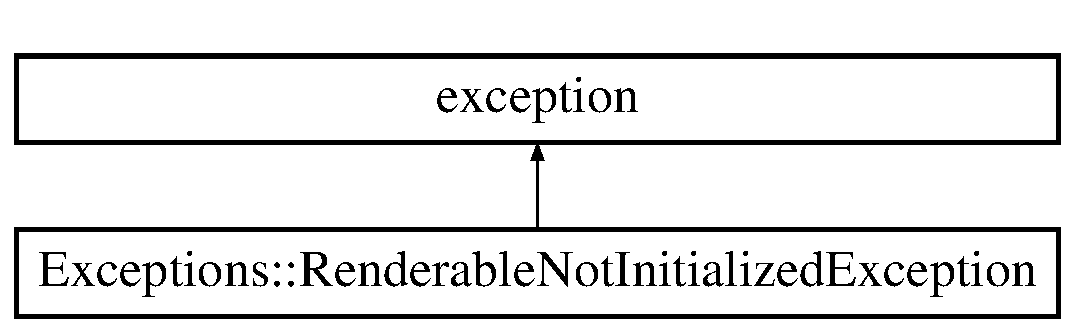
\includegraphics[height=2.000000cm]{class_exceptions_1_1_renderable_not_initialized_exception}
\end{center}
\end{figure}
\subsection*{Public Member Functions}
\begin{DoxyCompactItemize}
\item 
\hyperlink{class_exceptions_1_1_renderable_not_initialized_exception_a18c5b3c635950038831820df28b81bc5}{Renderable\+Not\+Initialized\+Exception} ()
\item 
virtual const char $\ast$ \hyperlink{class_exceptions_1_1_renderable_not_initialized_exception_a95b9337f6209c8df79b3120cd3e1ad5e}{what} () const   throw ()
\end{DoxyCompactItemize}


\subsection{Constructor \& Destructor Documentation}
\hypertarget{class_exceptions_1_1_renderable_not_initialized_exception_a18c5b3c635950038831820df28b81bc5}{}\index{Exceptions\+::\+Renderable\+Not\+Initialized\+Exception@{Exceptions\+::\+Renderable\+Not\+Initialized\+Exception}!Renderable\+Not\+Initialized\+Exception@{Renderable\+Not\+Initialized\+Exception}}
\index{Renderable\+Not\+Initialized\+Exception@{Renderable\+Not\+Initialized\+Exception}!Exceptions\+::\+Renderable\+Not\+Initialized\+Exception@{Exceptions\+::\+Renderable\+Not\+Initialized\+Exception}}
\subsubsection[{Renderable\+Not\+Initialized\+Exception}]{\setlength{\rightskip}{0pt plus 5cm}Exceptions\+::\+Renderable\+Not\+Initialized\+Exception\+::\+Renderable\+Not\+Initialized\+Exception (
\begin{DoxyParamCaption}
{}
\end{DoxyParamCaption}
)\hspace{0.3cm}{\ttfamily [inline]}}\label{class_exceptions_1_1_renderable_not_initialized_exception_a18c5b3c635950038831820df28b81bc5}


\subsection{Member Function Documentation}
\hypertarget{class_exceptions_1_1_renderable_not_initialized_exception_a95b9337f6209c8df79b3120cd3e1ad5e}{}\index{Exceptions\+::\+Renderable\+Not\+Initialized\+Exception@{Exceptions\+::\+Renderable\+Not\+Initialized\+Exception}!what@{what}}
\index{what@{what}!Exceptions\+::\+Renderable\+Not\+Initialized\+Exception@{Exceptions\+::\+Renderable\+Not\+Initialized\+Exception}}
\subsubsection[{what}]{\setlength{\rightskip}{0pt plus 5cm}virtual const char$\ast$ Exceptions\+::\+Renderable\+Not\+Initialized\+Exception\+::what (
\begin{DoxyParamCaption}
{}
\end{DoxyParamCaption}
) const throw  ) \hspace{0.3cm}{\ttfamily [inline]}, {\ttfamily [virtual]}}\label{class_exceptions_1_1_renderable_not_initialized_exception_a95b9337f6209c8df79b3120cd3e1ad5e}


The documentation for this class was generated from the following file\+:\begin{DoxyCompactItemize}
\item 
src/exceptions/\hyperlink{renderable__not__initialized__exception_8h}{renderable\+\_\+not\+\_\+initialized\+\_\+exception.\+h}\end{DoxyCompactItemize}

\hypertarget{class_graphics_1_1_shader}{}\section{Graphics\+:\+:Shader Class Reference}
\label{class_graphics_1_1_shader}\index{Graphics\+::\+Shader@{Graphics\+::\+Shader}}


{\ttfamily \#include $<$shader.\+h$>$}

\subsection*{Public Member Functions}
\begin{DoxyCompactItemize}
\item 
\hyperlink{class_graphics_1_1_shader_a8160ac75561d286213ec65ec30d9eeb0}{Shader} ()=delete
\item 
\hyperlink{class_graphics_1_1_shader_aef598fb3433acea1aff5e57499d08fed}{Shader} (const unsigned int vertex\+\_\+program, const unsigned int fragment\+\_\+program, const unsigned int geometry\+\_\+program=0)
\item 
const unsigned int \hyperlink{class_graphics_1_1_shader_a8310ca4e5e8dba64d1ad3636bada078b}{get\+Handle} () const noexcept
\item 
void \hyperlink{class_graphics_1_1_shader_a564d1802984fc0501f33528e8fe5aad3}{use\+Program} () const 
\item 
{\footnotesize template$<$class T $>$ }\\void \hyperlink{class_graphics_1_1_shader_a78f6ffc5d8fc4d3eee3189dae6e8434e}{set\+Uniform} (const std\+::string \&name, const T \&value)
\item 
{\footnotesize template$<$$>$ }\\void \hyperlink{class_graphics_1_1_shader_ae87e687bdc5b41e7162a3fd17cbe4b8c}{set\+Uniform} (const std\+::string \&name, const float \&data)
\item 
{\footnotesize template$<$$>$ }\\void \hyperlink{class_graphics_1_1_shader_a053a18f48bf33e427ae912e420f41300}{set\+Uniform} (const std\+::string \&name, const int \&data)
\item 
{\footnotesize template$<$$>$ }\\void \hyperlink{class_graphics_1_1_shader_abe8990b3404bfedef5a29d7557bf2ad8}{set\+Uniform} (const std\+::string \&name, const unsigned int \&data)
\item 
{\footnotesize template$<$$>$ }\\void \hyperlink{class_graphics_1_1_shader_a70df2013998b9cb0efce4bb3177c9599}{set\+Uniform} (const std\+::string \&name, const bool \&data)
\end{DoxyCompactItemize}
\subsection*{Private Attributes}
\begin{DoxyCompactItemize}
\item 
unsigned int \hyperlink{class_graphics_1_1_shader_a8e40ca5eb9880e84c29366dbe626c081}{program\+\_\+object}
\item 
std\+::map$<$ std\+::string, int $>$ \hyperlink{class_graphics_1_1_shader_a71b17a1ca67b9315b0aa44bb984a8617}{name\+\_\+to\+\_\+location}
\item 
std\+::map$<$ std\+::string, G\+Lenum $>$ \hyperlink{class_graphics_1_1_shader_a591f5dbbfbb6a851fb9bd88a91c17135}{name\+\_\+to\+\_\+type}
\end{DoxyCompactItemize}


\subsection{Constructor \& Destructor Documentation}
\hypertarget{class_graphics_1_1_shader_a8160ac75561d286213ec65ec30d9eeb0}{}\index{Graphics\+::\+Shader@{Graphics\+::\+Shader}!Shader@{Shader}}
\index{Shader@{Shader}!Graphics\+::\+Shader@{Graphics\+::\+Shader}}
\subsubsection[{Shader}]{\setlength{\rightskip}{0pt plus 5cm}Graphics\+::\+Shader\+::\+Shader (
\begin{DoxyParamCaption}
{}
\end{DoxyParamCaption}
)\hspace{0.3cm}{\ttfamily [delete]}}\label{class_graphics_1_1_shader_a8160ac75561d286213ec65ec30d9eeb0}
\hypertarget{class_graphics_1_1_shader_aef598fb3433acea1aff5e57499d08fed}{}\index{Graphics\+::\+Shader@{Graphics\+::\+Shader}!Shader@{Shader}}
\index{Shader@{Shader}!Graphics\+::\+Shader@{Graphics\+::\+Shader}}
\subsubsection[{Shader}]{\setlength{\rightskip}{0pt plus 5cm}Graphics\+::\+Shader\+::\+Shader (
\begin{DoxyParamCaption}
\item[{const unsigned int}]{vertex\+\_\+program, }
\item[{const unsigned int}]{fragment\+\_\+program, }
\item[{const unsigned int}]{geometry\+\_\+program = {\ttfamily 0}}
\end{DoxyParamCaption}
)}\label{class_graphics_1_1_shader_aef598fb3433acea1aff5e57499d08fed}


\subsection{Member Function Documentation}
\hypertarget{class_graphics_1_1_shader_a8310ca4e5e8dba64d1ad3636bada078b}{}\index{Graphics\+::\+Shader@{Graphics\+::\+Shader}!get\+Handle@{get\+Handle}}
\index{get\+Handle@{get\+Handle}!Graphics\+::\+Shader@{Graphics\+::\+Shader}}
\subsubsection[{get\+Handle}]{\setlength{\rightskip}{0pt plus 5cm}const unsigned int Graphics\+::\+Shader\+::get\+Handle (
\begin{DoxyParamCaption}
{}
\end{DoxyParamCaption}
) const\hspace{0.3cm}{\ttfamily [noexcept]}}\label{class_graphics_1_1_shader_a8310ca4e5e8dba64d1ad3636bada078b}
\hypertarget{class_graphics_1_1_shader_a78f6ffc5d8fc4d3eee3189dae6e8434e}{}\index{Graphics\+::\+Shader@{Graphics\+::\+Shader}!set\+Uniform@{set\+Uniform}}
\index{set\+Uniform@{set\+Uniform}!Graphics\+::\+Shader@{Graphics\+::\+Shader}}
\subsubsection[{set\+Uniform}]{\setlength{\rightskip}{0pt plus 5cm}template$<$class T $>$ void Graphics\+::\+Shader\+::set\+Uniform (
\begin{DoxyParamCaption}
\item[{const std\+::string \&}]{name, }
\item[{const T \&}]{value}
\end{DoxyParamCaption}
)}\label{class_graphics_1_1_shader_a78f6ffc5d8fc4d3eee3189dae6e8434e}
\hypertarget{class_graphics_1_1_shader_ae87e687bdc5b41e7162a3fd17cbe4b8c}{}\index{Graphics\+::\+Shader@{Graphics\+::\+Shader}!set\+Uniform@{set\+Uniform}}
\index{set\+Uniform@{set\+Uniform}!Graphics\+::\+Shader@{Graphics\+::\+Shader}}
\subsubsection[{set\+Uniform}]{\setlength{\rightskip}{0pt plus 5cm}template$<$$>$ void Graphics\+::\+Shader\+::set\+Uniform (
\begin{DoxyParamCaption}
\item[{const std\+::string \&}]{name, }
\item[{const float \&}]{data}
\end{DoxyParamCaption}
)}\label{class_graphics_1_1_shader_ae87e687bdc5b41e7162a3fd17cbe4b8c}
\hypertarget{class_graphics_1_1_shader_a053a18f48bf33e427ae912e420f41300}{}\index{Graphics\+::\+Shader@{Graphics\+::\+Shader}!set\+Uniform@{set\+Uniform}}
\index{set\+Uniform@{set\+Uniform}!Graphics\+::\+Shader@{Graphics\+::\+Shader}}
\subsubsection[{set\+Uniform}]{\setlength{\rightskip}{0pt plus 5cm}template$<$$>$ void Graphics\+::\+Shader\+::set\+Uniform (
\begin{DoxyParamCaption}
\item[{const std\+::string \&}]{name, }
\item[{const int \&}]{data}
\end{DoxyParamCaption}
)}\label{class_graphics_1_1_shader_a053a18f48bf33e427ae912e420f41300}
\hypertarget{class_graphics_1_1_shader_abe8990b3404bfedef5a29d7557bf2ad8}{}\index{Graphics\+::\+Shader@{Graphics\+::\+Shader}!set\+Uniform@{set\+Uniform}}
\index{set\+Uniform@{set\+Uniform}!Graphics\+::\+Shader@{Graphics\+::\+Shader}}
\subsubsection[{set\+Uniform}]{\setlength{\rightskip}{0pt plus 5cm}template$<$$>$ void Graphics\+::\+Shader\+::set\+Uniform (
\begin{DoxyParamCaption}
\item[{const std\+::string \&}]{name, }
\item[{const unsigned int \&}]{data}
\end{DoxyParamCaption}
)}\label{class_graphics_1_1_shader_abe8990b3404bfedef5a29d7557bf2ad8}
\hypertarget{class_graphics_1_1_shader_a70df2013998b9cb0efce4bb3177c9599}{}\index{Graphics\+::\+Shader@{Graphics\+::\+Shader}!set\+Uniform@{set\+Uniform}}
\index{set\+Uniform@{set\+Uniform}!Graphics\+::\+Shader@{Graphics\+::\+Shader}}
\subsubsection[{set\+Uniform}]{\setlength{\rightskip}{0pt plus 5cm}template$<$$>$ void Graphics\+::\+Shader\+::set\+Uniform (
\begin{DoxyParamCaption}
\item[{const std\+::string \&}]{name, }
\item[{const bool \&}]{data}
\end{DoxyParamCaption}
)}\label{class_graphics_1_1_shader_a70df2013998b9cb0efce4bb3177c9599}
\hypertarget{class_graphics_1_1_shader_a564d1802984fc0501f33528e8fe5aad3}{}\index{Graphics\+::\+Shader@{Graphics\+::\+Shader}!use\+Program@{use\+Program}}
\index{use\+Program@{use\+Program}!Graphics\+::\+Shader@{Graphics\+::\+Shader}}
\subsubsection[{use\+Program}]{\setlength{\rightskip}{0pt plus 5cm}void Graphics\+::\+Shader\+::use\+Program (
\begin{DoxyParamCaption}
{}
\end{DoxyParamCaption}
) const}\label{class_graphics_1_1_shader_a564d1802984fc0501f33528e8fe5aad3}


\subsection{Member Data Documentation}
\hypertarget{class_graphics_1_1_shader_a71b17a1ca67b9315b0aa44bb984a8617}{}\index{Graphics\+::\+Shader@{Graphics\+::\+Shader}!name\+\_\+to\+\_\+location@{name\+\_\+to\+\_\+location}}
\index{name\+\_\+to\+\_\+location@{name\+\_\+to\+\_\+location}!Graphics\+::\+Shader@{Graphics\+::\+Shader}}
\subsubsection[{name\+\_\+to\+\_\+location}]{\setlength{\rightskip}{0pt plus 5cm}std\+::map$<$std\+::string, int$>$ Graphics\+::\+Shader\+::name\+\_\+to\+\_\+location\hspace{0.3cm}{\ttfamily [private]}}\label{class_graphics_1_1_shader_a71b17a1ca67b9315b0aa44bb984a8617}
\hypertarget{class_graphics_1_1_shader_a591f5dbbfbb6a851fb9bd88a91c17135}{}\index{Graphics\+::\+Shader@{Graphics\+::\+Shader}!name\+\_\+to\+\_\+type@{name\+\_\+to\+\_\+type}}
\index{name\+\_\+to\+\_\+type@{name\+\_\+to\+\_\+type}!Graphics\+::\+Shader@{Graphics\+::\+Shader}}
\subsubsection[{name\+\_\+to\+\_\+type}]{\setlength{\rightskip}{0pt plus 5cm}std\+::map$<$std\+::string, G\+Lenum$>$ Graphics\+::\+Shader\+::name\+\_\+to\+\_\+type\hspace{0.3cm}{\ttfamily [private]}}\label{class_graphics_1_1_shader_a591f5dbbfbb6a851fb9bd88a91c17135}
\hypertarget{class_graphics_1_1_shader_a8e40ca5eb9880e84c29366dbe626c081}{}\index{Graphics\+::\+Shader@{Graphics\+::\+Shader}!program\+\_\+object@{program\+\_\+object}}
\index{program\+\_\+object@{program\+\_\+object}!Graphics\+::\+Shader@{Graphics\+::\+Shader}}
\subsubsection[{program\+\_\+object}]{\setlength{\rightskip}{0pt plus 5cm}unsigned int Graphics\+::\+Shader\+::program\+\_\+object\hspace{0.3cm}{\ttfamily [private]}}\label{class_graphics_1_1_shader_a8e40ca5eb9880e84c29366dbe626c081}


The documentation for this class was generated from the following files\+:\begin{DoxyCompactItemize}
\item 
src/graphics/\hyperlink{shader_8h}{shader.\+h}\item 
src/graphics/\hyperlink{shader_8cpp}{shader.\+cpp}\end{DoxyCompactItemize}

\hypertarget{class_exceptions_1_1_shader_compilation_exception}{}\section{Exceptions\+:\+:Shader\+Compilation\+Exception Class Reference}
\label{class_exceptions_1_1_shader_compilation_exception}\index{Exceptions\+::\+Shader\+Compilation\+Exception@{Exceptions\+::\+Shader\+Compilation\+Exception}}


{\ttfamily \#include $<$shader\+\_\+compilation\+\_\+exception.\+h$>$}

Inheritance diagram for Exceptions\+:\+:Shader\+Compilation\+Exception\+:\begin{figure}[H]
\begin{center}
\leavevmode
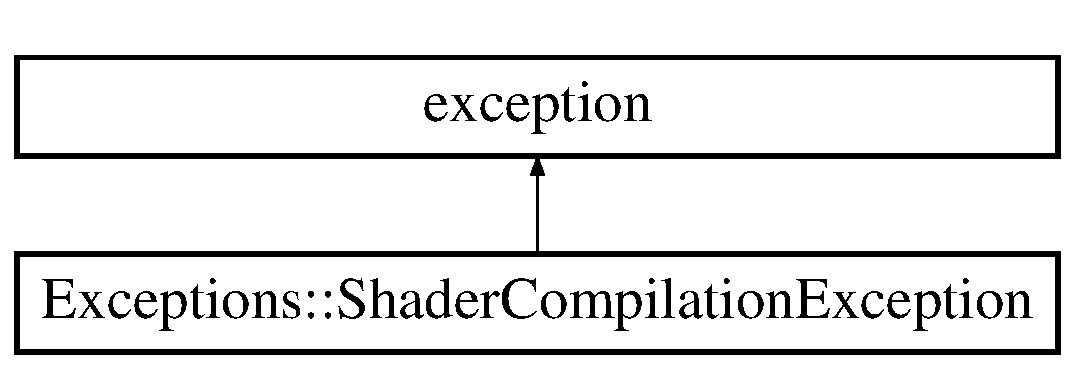
\includegraphics[height=2.000000cm]{class_exceptions_1_1_shader_compilation_exception}
\end{center}
\end{figure}
\subsection*{Public Member Functions}
\begin{DoxyCompactItemize}
\item 
\hyperlink{class_exceptions_1_1_shader_compilation_exception_a54bfc3c68f7c4aa388fbf73551cda495}{Shader\+Compilation\+Exception} (const std\+::string \&filename)
\item 
virtual const char $\ast$ \hyperlink{class_exceptions_1_1_shader_compilation_exception_ae5d257d5aea5325d820ec841747abe07}{what} () const   throw ()
\end{DoxyCompactItemize}
\subsection*{Private Attributes}
\begin{DoxyCompactItemize}
\item 
std\+::string \hyperlink{class_exceptions_1_1_shader_compilation_exception_a9762b7c686cc137596a40ad16d19a2f9}{shader\+\_\+filename}
\end{DoxyCompactItemize}


\subsection{Constructor \& Destructor Documentation}
\hypertarget{class_exceptions_1_1_shader_compilation_exception_a54bfc3c68f7c4aa388fbf73551cda495}{}\index{Exceptions\+::\+Shader\+Compilation\+Exception@{Exceptions\+::\+Shader\+Compilation\+Exception}!Shader\+Compilation\+Exception@{Shader\+Compilation\+Exception}}
\index{Shader\+Compilation\+Exception@{Shader\+Compilation\+Exception}!Exceptions\+::\+Shader\+Compilation\+Exception@{Exceptions\+::\+Shader\+Compilation\+Exception}}
\subsubsection[{Shader\+Compilation\+Exception}]{\setlength{\rightskip}{0pt plus 5cm}Exceptions\+::\+Shader\+Compilation\+Exception\+::\+Shader\+Compilation\+Exception (
\begin{DoxyParamCaption}
\item[{const std\+::string \&}]{filename}
\end{DoxyParamCaption}
)\hspace{0.3cm}{\ttfamily [inline]}}\label{class_exceptions_1_1_shader_compilation_exception_a54bfc3c68f7c4aa388fbf73551cda495}


\subsection{Member Function Documentation}
\hypertarget{class_exceptions_1_1_shader_compilation_exception_ae5d257d5aea5325d820ec841747abe07}{}\index{Exceptions\+::\+Shader\+Compilation\+Exception@{Exceptions\+::\+Shader\+Compilation\+Exception}!what@{what}}
\index{what@{what}!Exceptions\+::\+Shader\+Compilation\+Exception@{Exceptions\+::\+Shader\+Compilation\+Exception}}
\subsubsection[{what}]{\setlength{\rightskip}{0pt plus 5cm}virtual const char$\ast$ Exceptions\+::\+Shader\+Compilation\+Exception\+::what (
\begin{DoxyParamCaption}
{}
\end{DoxyParamCaption}
) const throw  ) \hspace{0.3cm}{\ttfamily [inline]}, {\ttfamily [virtual]}}\label{class_exceptions_1_1_shader_compilation_exception_ae5d257d5aea5325d820ec841747abe07}


\subsection{Member Data Documentation}
\hypertarget{class_exceptions_1_1_shader_compilation_exception_a9762b7c686cc137596a40ad16d19a2f9}{}\index{Exceptions\+::\+Shader\+Compilation\+Exception@{Exceptions\+::\+Shader\+Compilation\+Exception}!shader\+\_\+filename@{shader\+\_\+filename}}
\index{shader\+\_\+filename@{shader\+\_\+filename}!Exceptions\+::\+Shader\+Compilation\+Exception@{Exceptions\+::\+Shader\+Compilation\+Exception}}
\subsubsection[{shader\+\_\+filename}]{\setlength{\rightskip}{0pt plus 5cm}std\+::string Exceptions\+::\+Shader\+Compilation\+Exception\+::shader\+\_\+filename\hspace{0.3cm}{\ttfamily [private]}}\label{class_exceptions_1_1_shader_compilation_exception_a9762b7c686cc137596a40ad16d19a2f9}


The documentation for this class was generated from the following file\+:\begin{DoxyCompactItemize}
\item 
src/exceptions/\hyperlink{shader__compilation__exception_8h}{shader\+\_\+compilation\+\_\+exception.\+h}\end{DoxyCompactItemize}

\hypertarget{class_graphics_1_1_shader_manager}{}\section{Graphics\+:\+:Shader\+Manager Class Reference}
\label{class_graphics_1_1_shader_manager}\index{Graphics\+::\+Shader\+Manager@{Graphics\+::\+Shader\+Manager}}


{\ttfamily \#include $<$shader\+\_\+manager.\+h$>$}

\subsection*{Public Member Functions}
\begin{DoxyCompactItemize}
\item 
\hyperlink{class_graphics_1_1_shader_manager_ac5f14e07d3b7bffa4b4cf63d9c4fb3a7}{Shader\+Manager} ()
\item 
\hyperlink{class_graphics_1_1_shader_manager_a1846632f26cfcb4907844716f23e0540}{$\sim$\+Shader\+Manager} ()
\item 
const bool \hyperlink{class_graphics_1_1_shader_manager_a29234192f964ad1d9da812e8ceab008f}{load\+Shader} (const std\+::string \&name, const bool geometry\+\_\+shader=false)
\item 
const bool \hyperlink{class_graphics_1_1_shader_manager_a0cd014938152e36fd81717dadd7e390a}{load\+Shader} (const std\+::string \&name, const std\+::string \&vertex\+\_\+filename, const std\+::string \&fragment\+\_\+filename, const std\+::string \&geometry\+\_\+filename)
\item 
const std\+::shared\+\_\+ptr$<$ \hyperlink{class_graphics_1_1_shader}{Shader} $>$ \hyperlink{class_graphics_1_1_shader_manager_a4a3c0f369be06a34a8e44ad8a41862a4}{operator\mbox{[}$\,$\mbox{]}} (const std\+::string \&name) const 
\item 
const std\+::shared\+\_\+ptr$<$ \hyperlink{class_graphics_1_1_shader}{Shader} $>$ \hyperlink{class_graphics_1_1_shader_manager_a8c82c5f8d73dbb9ec3038b2db71add41}{get\+Shader} (const std\+::string \&name) const 
\end{DoxyCompactItemize}
\subsection*{Static Public Attributes}
\begin{DoxyCompactItemize}
\item 
static char const $\ast$ \hyperlink{class_graphics_1_1_shader_manager_abb954de5b5b6bc56d568e20b478f0712}{V\+E\+R\+T\+E\+X\+\_\+\+E\+X\+T\+E\+N\+S\+I\+O\+N} = \char`\"{}.vert\char`\"{}
\item 
static char const $\ast$ \hyperlink{class_graphics_1_1_shader_manager_aa3ad06b558229fe4d4d4ebbabfe9ca48}{F\+R\+A\+G\+M\+E\+N\+T\+\_\+\+E\+X\+T\+E\+N\+S\+I\+O\+N} = \char`\"{}.frag\char`\"{}
\item 
static char const $\ast$ \hyperlink{class_graphics_1_1_shader_manager_a66cf54024f2f1e51db6f5afccbcba67e}{G\+E\+O\+M\+E\+T\+R\+Y\+\_\+\+E\+X\+T\+E\+N\+S\+I\+O\+N} = \char`\"{}.geom\char`\"{}
\item 
static char const $\ast$ \hyperlink{class_graphics_1_1_shader_manager_ad3cef3602a2a0205064bdff0ac9437a8}{S\+H\+A\+D\+E\+R\+\_\+\+D\+I\+R\+E\+C\+T\+O\+R\+Y} = \char`\"{}./shaders/\char`\"{}
\end{DoxyCompactItemize}
\subsection*{Private Attributes}
\begin{DoxyCompactItemize}
\item 
std\+::map$<$ std\+::string, std\+::shared\+\_\+ptr$<$ \hyperlink{class_graphics_1_1_shader}{Shader} $>$ $>$ \hyperlink{class_graphics_1_1_shader_manager_a5cada9e001d0b2ead2bfb7a0ef37be66}{shaders\+\_\+to\+\_\+names}
\end{DoxyCompactItemize}


\subsection{Constructor \& Destructor Documentation}
\hypertarget{class_graphics_1_1_shader_manager_ac5f14e07d3b7bffa4b4cf63d9c4fb3a7}{}\index{Graphics\+::\+Shader\+Manager@{Graphics\+::\+Shader\+Manager}!Shader\+Manager@{Shader\+Manager}}
\index{Shader\+Manager@{Shader\+Manager}!Graphics\+::\+Shader\+Manager@{Graphics\+::\+Shader\+Manager}}
\subsubsection[{Shader\+Manager}]{\setlength{\rightskip}{0pt plus 5cm}Graphics\+::\+Shader\+Manager\+::\+Shader\+Manager (
\begin{DoxyParamCaption}
{}
\end{DoxyParamCaption}
)}\label{class_graphics_1_1_shader_manager_ac5f14e07d3b7bffa4b4cf63d9c4fb3a7}
\hypertarget{class_graphics_1_1_shader_manager_a1846632f26cfcb4907844716f23e0540}{}\index{Graphics\+::\+Shader\+Manager@{Graphics\+::\+Shader\+Manager}!````~Shader\+Manager@{$\sim$\+Shader\+Manager}}
\index{````~Shader\+Manager@{$\sim$\+Shader\+Manager}!Graphics\+::\+Shader\+Manager@{Graphics\+::\+Shader\+Manager}}
\subsubsection[{$\sim$\+Shader\+Manager}]{\setlength{\rightskip}{0pt plus 5cm}Graphics\+::\+Shader\+Manager\+::$\sim$\+Shader\+Manager (
\begin{DoxyParamCaption}
{}
\end{DoxyParamCaption}
)}\label{class_graphics_1_1_shader_manager_a1846632f26cfcb4907844716f23e0540}


\subsection{Member Function Documentation}
\hypertarget{class_graphics_1_1_shader_manager_a8c82c5f8d73dbb9ec3038b2db71add41}{}\index{Graphics\+::\+Shader\+Manager@{Graphics\+::\+Shader\+Manager}!get\+Shader@{get\+Shader}}
\index{get\+Shader@{get\+Shader}!Graphics\+::\+Shader\+Manager@{Graphics\+::\+Shader\+Manager}}
\subsubsection[{get\+Shader}]{\setlength{\rightskip}{0pt plus 5cm}const std\+::shared\+\_\+ptr$<$ {\bf Shader} $>$ Graphics\+::\+Shader\+Manager\+::get\+Shader (
\begin{DoxyParamCaption}
\item[{const std\+::string \&}]{name}
\end{DoxyParamCaption}
) const}\label{class_graphics_1_1_shader_manager_a8c82c5f8d73dbb9ec3038b2db71add41}
\hypertarget{class_graphics_1_1_shader_manager_a29234192f964ad1d9da812e8ceab008f}{}\index{Graphics\+::\+Shader\+Manager@{Graphics\+::\+Shader\+Manager}!load\+Shader@{load\+Shader}}
\index{load\+Shader@{load\+Shader}!Graphics\+::\+Shader\+Manager@{Graphics\+::\+Shader\+Manager}}
\subsubsection[{load\+Shader}]{\setlength{\rightskip}{0pt plus 5cm}const bool Graphics\+::\+Shader\+Manager\+::load\+Shader (
\begin{DoxyParamCaption}
\item[{const std\+::string \&}]{name, }
\item[{const bool}]{geometry\+\_\+shader = {\ttfamily false}}
\end{DoxyParamCaption}
)}\label{class_graphics_1_1_shader_manager_a29234192f964ad1d9da812e8ceab008f}
\hypertarget{class_graphics_1_1_shader_manager_a0cd014938152e36fd81717dadd7e390a}{}\index{Graphics\+::\+Shader\+Manager@{Graphics\+::\+Shader\+Manager}!load\+Shader@{load\+Shader}}
\index{load\+Shader@{load\+Shader}!Graphics\+::\+Shader\+Manager@{Graphics\+::\+Shader\+Manager}}
\subsubsection[{load\+Shader}]{\setlength{\rightskip}{0pt plus 5cm}const bool Graphics\+::\+Shader\+Manager\+::load\+Shader (
\begin{DoxyParamCaption}
\item[{const std\+::string \&}]{name, }
\item[{const std\+::string \&}]{vertex\+\_\+filename, }
\item[{const std\+::string \&}]{fragment\+\_\+filename, }
\item[{const std\+::string \&}]{geometry\+\_\+filename}
\end{DoxyParamCaption}
)}\label{class_graphics_1_1_shader_manager_a0cd014938152e36fd81717dadd7e390a}
\hypertarget{class_graphics_1_1_shader_manager_a4a3c0f369be06a34a8e44ad8a41862a4}{}\index{Graphics\+::\+Shader\+Manager@{Graphics\+::\+Shader\+Manager}!operator\mbox{[}$\,$\mbox{]}@{operator[]}}
\index{operator\mbox{[}$\,$\mbox{]}@{operator[]}!Graphics\+::\+Shader\+Manager@{Graphics\+::\+Shader\+Manager}}
\subsubsection[{operator[]}]{\setlength{\rightskip}{0pt plus 5cm}const std\+::shared\+\_\+ptr$<$ {\bf Shader} $>$ Graphics\+::\+Shader\+Manager\+::operator\mbox{[}$\,$\mbox{]} (
\begin{DoxyParamCaption}
\item[{const std\+::string \&}]{name}
\end{DoxyParamCaption}
) const}\label{class_graphics_1_1_shader_manager_a4a3c0f369be06a34a8e44ad8a41862a4}


\subsection{Member Data Documentation}
\hypertarget{class_graphics_1_1_shader_manager_aa3ad06b558229fe4d4d4ebbabfe9ca48}{}\index{Graphics\+::\+Shader\+Manager@{Graphics\+::\+Shader\+Manager}!F\+R\+A\+G\+M\+E\+N\+T\+\_\+\+E\+X\+T\+E\+N\+S\+I\+O\+N@{F\+R\+A\+G\+M\+E\+N\+T\+\_\+\+E\+X\+T\+E\+N\+S\+I\+O\+N}}
\index{F\+R\+A\+G\+M\+E\+N\+T\+\_\+\+E\+X\+T\+E\+N\+S\+I\+O\+N@{F\+R\+A\+G\+M\+E\+N\+T\+\_\+\+E\+X\+T\+E\+N\+S\+I\+O\+N}!Graphics\+::\+Shader\+Manager@{Graphics\+::\+Shader\+Manager}}
\subsubsection[{F\+R\+A\+G\+M\+E\+N\+T\+\_\+\+E\+X\+T\+E\+N\+S\+I\+O\+N}]{\setlength{\rightskip}{0pt plus 5cm}char const $\ast$ Graphics\+::\+Shader\+Manager\+::\+F\+R\+A\+G\+M\+E\+N\+T\+\_\+\+E\+X\+T\+E\+N\+S\+I\+O\+N = \char`\"{}.frag\char`\"{}\hspace{0.3cm}{\ttfamily [static]}}\label{class_graphics_1_1_shader_manager_aa3ad06b558229fe4d4d4ebbabfe9ca48}
\hypertarget{class_graphics_1_1_shader_manager_a66cf54024f2f1e51db6f5afccbcba67e}{}\index{Graphics\+::\+Shader\+Manager@{Graphics\+::\+Shader\+Manager}!G\+E\+O\+M\+E\+T\+R\+Y\+\_\+\+E\+X\+T\+E\+N\+S\+I\+O\+N@{G\+E\+O\+M\+E\+T\+R\+Y\+\_\+\+E\+X\+T\+E\+N\+S\+I\+O\+N}}
\index{G\+E\+O\+M\+E\+T\+R\+Y\+\_\+\+E\+X\+T\+E\+N\+S\+I\+O\+N@{G\+E\+O\+M\+E\+T\+R\+Y\+\_\+\+E\+X\+T\+E\+N\+S\+I\+O\+N}!Graphics\+::\+Shader\+Manager@{Graphics\+::\+Shader\+Manager}}
\subsubsection[{G\+E\+O\+M\+E\+T\+R\+Y\+\_\+\+E\+X\+T\+E\+N\+S\+I\+O\+N}]{\setlength{\rightskip}{0pt plus 5cm}char const $\ast$ Graphics\+::\+Shader\+Manager\+::\+G\+E\+O\+M\+E\+T\+R\+Y\+\_\+\+E\+X\+T\+E\+N\+S\+I\+O\+N = \char`\"{}.geom\char`\"{}\hspace{0.3cm}{\ttfamily [static]}}\label{class_graphics_1_1_shader_manager_a66cf54024f2f1e51db6f5afccbcba67e}
\hypertarget{class_graphics_1_1_shader_manager_ad3cef3602a2a0205064bdff0ac9437a8}{}\index{Graphics\+::\+Shader\+Manager@{Graphics\+::\+Shader\+Manager}!S\+H\+A\+D\+E\+R\+\_\+\+D\+I\+R\+E\+C\+T\+O\+R\+Y@{S\+H\+A\+D\+E\+R\+\_\+\+D\+I\+R\+E\+C\+T\+O\+R\+Y}}
\index{S\+H\+A\+D\+E\+R\+\_\+\+D\+I\+R\+E\+C\+T\+O\+R\+Y@{S\+H\+A\+D\+E\+R\+\_\+\+D\+I\+R\+E\+C\+T\+O\+R\+Y}!Graphics\+::\+Shader\+Manager@{Graphics\+::\+Shader\+Manager}}
\subsubsection[{S\+H\+A\+D\+E\+R\+\_\+\+D\+I\+R\+E\+C\+T\+O\+R\+Y}]{\setlength{\rightskip}{0pt plus 5cm}char const $\ast$ Graphics\+::\+Shader\+Manager\+::\+S\+H\+A\+D\+E\+R\+\_\+\+D\+I\+R\+E\+C\+T\+O\+R\+Y = \char`\"{}./shaders/\char`\"{}\hspace{0.3cm}{\ttfamily [static]}}\label{class_graphics_1_1_shader_manager_ad3cef3602a2a0205064bdff0ac9437a8}
\hypertarget{class_graphics_1_1_shader_manager_a5cada9e001d0b2ead2bfb7a0ef37be66}{}\index{Graphics\+::\+Shader\+Manager@{Graphics\+::\+Shader\+Manager}!shaders\+\_\+to\+\_\+names@{shaders\+\_\+to\+\_\+names}}
\index{shaders\+\_\+to\+\_\+names@{shaders\+\_\+to\+\_\+names}!Graphics\+::\+Shader\+Manager@{Graphics\+::\+Shader\+Manager}}
\subsubsection[{shaders\+\_\+to\+\_\+names}]{\setlength{\rightskip}{0pt plus 5cm}std\+::map$<$std\+::string, std\+::shared\+\_\+ptr$<${\bf Shader}$>$ $>$ Graphics\+::\+Shader\+Manager\+::shaders\+\_\+to\+\_\+names\hspace{0.3cm}{\ttfamily [private]}}\label{class_graphics_1_1_shader_manager_a5cada9e001d0b2ead2bfb7a0ef37be66}
\hypertarget{class_graphics_1_1_shader_manager_abb954de5b5b6bc56d568e20b478f0712}{}\index{Graphics\+::\+Shader\+Manager@{Graphics\+::\+Shader\+Manager}!V\+E\+R\+T\+E\+X\+\_\+\+E\+X\+T\+E\+N\+S\+I\+O\+N@{V\+E\+R\+T\+E\+X\+\_\+\+E\+X\+T\+E\+N\+S\+I\+O\+N}}
\index{V\+E\+R\+T\+E\+X\+\_\+\+E\+X\+T\+E\+N\+S\+I\+O\+N@{V\+E\+R\+T\+E\+X\+\_\+\+E\+X\+T\+E\+N\+S\+I\+O\+N}!Graphics\+::\+Shader\+Manager@{Graphics\+::\+Shader\+Manager}}
\subsubsection[{V\+E\+R\+T\+E\+X\+\_\+\+E\+X\+T\+E\+N\+S\+I\+O\+N}]{\setlength{\rightskip}{0pt plus 5cm}char const $\ast$ Graphics\+::\+Shader\+Manager\+::\+V\+E\+R\+T\+E\+X\+\_\+\+E\+X\+T\+E\+N\+S\+I\+O\+N = \char`\"{}.vert\char`\"{}\hspace{0.3cm}{\ttfamily [static]}}\label{class_graphics_1_1_shader_manager_abb954de5b5b6bc56d568e20b478f0712}


The documentation for this class was generated from the following files\+:\begin{DoxyCompactItemize}
\item 
src/graphics/\hyperlink{shader__manager_8h}{shader\+\_\+manager.\+h}\item 
src/graphics/\hyperlink{shader__manager_8cpp}{shader\+\_\+manager.\+cpp}\end{DoxyCompactItemize}

\hypertarget{class_sprite}{}\section{Sprite Class Reference}
\label{class_sprite}\index{Sprite@{Sprite}}


{\ttfamily \#include $<$sprite.\+h$>$}

Inheritance diagram for Sprite\+:\begin{figure}[H]
\begin{center}
\leavevmode
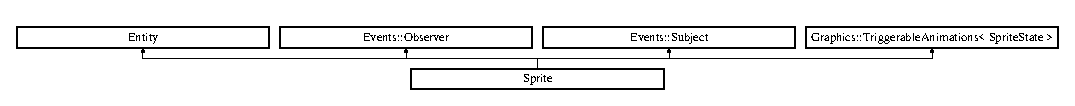
\includegraphics[height=0.972222cm]{class_sprite}
\end{center}
\end{figure}
\subsection*{Public Member Functions}
\begin{DoxyCompactItemize}
\item 
\hyperlink{class_sprite_a12cba3ac1868418add3c4d95ce87e615}{Sprite} ()
\item 
void \hyperlink{class_sprite_a86d7cca33da7b1e2681da6bd094be088}{on\+Notify} (const \hyperlink{class_events_1_1_event}{Events\+::\+Event} \&event) override
\item 
void \hyperlink{class_sprite_a0db72afea03d07a957b1bee8a0828c2d}{on\+Update} (const float delta) override
\item 
void \hyperlink{class_sprite_afdefdcda4fb7de9ed10bb9571928f665}{on\+Start} () override
\item 
void \hyperlink{class_sprite_a974593031fb6e1a53883a588b7669422}{add\+Triggerable\+Tile} (const \hyperlink{sprite_8h_af7ccac6abcbe8bf213b36feaa7b69cda}{Sprite\+State} \&state, std\+::shared\+\_\+ptr$<$ \hyperlink{class_graphics_1_1_tile}{Graphics\+::\+Tile} $>$ tile)
\item 
void \hyperlink{class_sprite_a55be0cc7ccc4fb02d4e5c0c10cdd7c32}{set\+Moving\+Speed} (const float speed)
\item 
void \hyperlink{class_sprite_ae6dea1bbb49662ad95ad7fb4629bed54}{set\+Move\+Quantization} (const float number\+\_\+of\+\_\+tiles)
\item 
void \hyperlink{class_sprite_a02fea5f2c354539922212722aaa52dde}{stop\+Moving\+Left} ()
\item 
void \hyperlink{class_sprite_a2b32d9f2d5dad0992069fc0e41f18548}{move\+Left} ()
\item 
void \hyperlink{class_sprite_a6e003778e1db53846a484b0ce44fc1fe}{stop\+Moving\+Right} ()
\item 
void \hyperlink{class_sprite_a7de624519b1f7e754a4d26ba9fad2e6b}{move\+Right} ()
\item 
void \hyperlink{class_sprite_a03ac7597c67a532e3ba6f101670b55bd}{stop\+Moving\+Up} ()
\item 
void \hyperlink{class_sprite_ae8bd81da374569643dca0f473d6edb60}{move\+Up} ()
\item 
void \hyperlink{class_sprite_a029ed51250b9bfbe69e3de60fe533b5c}{stop\+Moving\+Down} ()
\item 
void \hyperlink{class_sprite_a558d8e35835a4a0c2ef6afdc7adc7309}{move\+Down} ()
\item 
std\+::list$<$ std\+::shared\+\_\+ptr$<$ \hyperlink{class_component}{Component} $>$ $>$ \hyperlink{class_sprite_a3d3ec9294747ab657db1ad2e6d0a15a5}{get\+Components} ()
\end{DoxyCompactItemize}
\subsection*{Private Attributes}
\begin{DoxyCompactItemize}
\item 
float \hyperlink{class_sprite_ad926ce6bee2f2fec7c919fc239a05562}{moving\+\_\+speed}
\item 
float \hyperlink{class_sprite_a6d0ab8736ed2427b9ae3784ec13559ac}{move\+\_\+quantization\+\_\+in\+\_\+tiles}
\item 
glm\+::vec2 \hyperlink{class_sprite_a3243ae10ccf1c0ffdd7318fd86031c4b}{current\+\_\+velocity}
\item 
glm\+::vec2 \hyperlink{class_sprite_a9f3431bd938e2f2097833bb014182db6}{next\+\_\+position}
\item 
bool \hyperlink{class_sprite_aa4bbce95c033a28b6fb7621d4bf669f0}{left\+\_\+down}
\item 
bool \hyperlink{class_sprite_a41fe0a8d0b923c47bdf6f99806f763f4}{up\+\_\+down}
\item 
bool \hyperlink{class_sprite_ab52c6db2e3784c0ef3c120cc758028e8}{down\+\_\+down}
\item 
bool \hyperlink{class_sprite_ad3df5ad11bc9883e55cfea8d48a7166f}{right\+\_\+down}
\end{DoxyCompactItemize}
\subsection*{Additional Inherited Members}


\subsection{Constructor \& Destructor Documentation}
\hypertarget{class_sprite_a12cba3ac1868418add3c4d95ce87e615}{}\index{Sprite@{Sprite}!Sprite@{Sprite}}
\index{Sprite@{Sprite}!Sprite@{Sprite}}
\subsubsection[{Sprite}]{\setlength{\rightskip}{0pt plus 5cm}Sprite\+::\+Sprite (
\begin{DoxyParamCaption}
{}
\end{DoxyParamCaption}
)}\label{class_sprite_a12cba3ac1868418add3c4d95ce87e615}


\subsection{Member Function Documentation}
\hypertarget{class_sprite_a974593031fb6e1a53883a588b7669422}{}\index{Sprite@{Sprite}!add\+Triggerable\+Tile@{add\+Triggerable\+Tile}}
\index{add\+Triggerable\+Tile@{add\+Triggerable\+Tile}!Sprite@{Sprite}}
\subsubsection[{add\+Triggerable\+Tile}]{\setlength{\rightskip}{0pt plus 5cm}void Sprite\+::add\+Triggerable\+Tile (
\begin{DoxyParamCaption}
\item[{const {\bf Sprite\+State} \&}]{state, }
\item[{std\+::shared\+\_\+ptr$<$ {\bf Graphics\+::\+Tile} $>$}]{tile}
\end{DoxyParamCaption}
)}\label{class_sprite_a974593031fb6e1a53883a588b7669422}
\hypertarget{class_sprite_a3d3ec9294747ab657db1ad2e6d0a15a5}{}\index{Sprite@{Sprite}!get\+Components@{get\+Components}}
\index{get\+Components@{get\+Components}!Sprite@{Sprite}}
\subsubsection[{get\+Components}]{\setlength{\rightskip}{0pt plus 5cm}std\+::list$<$ std\+::shared\+\_\+ptr$<$ {\bf Component} $>$ $>$ Sprite\+::get\+Components (
\begin{DoxyParamCaption}
{}
\end{DoxyParamCaption}
)}\label{class_sprite_a3d3ec9294747ab657db1ad2e6d0a15a5}
\hypertarget{class_sprite_a558d8e35835a4a0c2ef6afdc7adc7309}{}\index{Sprite@{Sprite}!move\+Down@{move\+Down}}
\index{move\+Down@{move\+Down}!Sprite@{Sprite}}
\subsubsection[{move\+Down}]{\setlength{\rightskip}{0pt plus 5cm}void Sprite\+::move\+Down (
\begin{DoxyParamCaption}
{}
\end{DoxyParamCaption}
)}\label{class_sprite_a558d8e35835a4a0c2ef6afdc7adc7309}
\hypertarget{class_sprite_a2b32d9f2d5dad0992069fc0e41f18548}{}\index{Sprite@{Sprite}!move\+Left@{move\+Left}}
\index{move\+Left@{move\+Left}!Sprite@{Sprite}}
\subsubsection[{move\+Left}]{\setlength{\rightskip}{0pt plus 5cm}void Sprite\+::move\+Left (
\begin{DoxyParamCaption}
{}
\end{DoxyParamCaption}
)}\label{class_sprite_a2b32d9f2d5dad0992069fc0e41f18548}
\hypertarget{class_sprite_a7de624519b1f7e754a4d26ba9fad2e6b}{}\index{Sprite@{Sprite}!move\+Right@{move\+Right}}
\index{move\+Right@{move\+Right}!Sprite@{Sprite}}
\subsubsection[{move\+Right}]{\setlength{\rightskip}{0pt plus 5cm}void Sprite\+::move\+Right (
\begin{DoxyParamCaption}
{}
\end{DoxyParamCaption}
)}\label{class_sprite_a7de624519b1f7e754a4d26ba9fad2e6b}
\hypertarget{class_sprite_ae8bd81da374569643dca0f473d6edb60}{}\index{Sprite@{Sprite}!move\+Up@{move\+Up}}
\index{move\+Up@{move\+Up}!Sprite@{Sprite}}
\subsubsection[{move\+Up}]{\setlength{\rightskip}{0pt plus 5cm}void Sprite\+::move\+Up (
\begin{DoxyParamCaption}
{}
\end{DoxyParamCaption}
)}\label{class_sprite_ae8bd81da374569643dca0f473d6edb60}
\hypertarget{class_sprite_a86d7cca33da7b1e2681da6bd094be088}{}\index{Sprite@{Sprite}!on\+Notify@{on\+Notify}}
\index{on\+Notify@{on\+Notify}!Sprite@{Sprite}}
\subsubsection[{on\+Notify}]{\setlength{\rightskip}{0pt plus 5cm}void Sprite\+::on\+Notify (
\begin{DoxyParamCaption}
\item[{const {\bf Events\+::\+Event} \&}]{event}
\end{DoxyParamCaption}
)\hspace{0.3cm}{\ttfamily [override]}, {\ttfamily [virtual]}}\label{class_sprite_a86d7cca33da7b1e2681da6bd094be088}


Implements \hyperlink{class_events_1_1_observer_ad10e3ade9e803e9f706c5799da1d6525}{Events\+::\+Observer}.

\hypertarget{class_sprite_afdefdcda4fb7de9ed10bb9571928f665}{}\index{Sprite@{Sprite}!on\+Start@{on\+Start}}
\index{on\+Start@{on\+Start}!Sprite@{Sprite}}
\subsubsection[{on\+Start}]{\setlength{\rightskip}{0pt plus 5cm}void Sprite\+::on\+Start (
\begin{DoxyParamCaption}
{}
\end{DoxyParamCaption}
)\hspace{0.3cm}{\ttfamily [override]}, {\ttfamily [virtual]}}\label{class_sprite_afdefdcda4fb7de9ed10bb9571928f665}


Reimplemented from \hyperlink{class_entity_afe788ab09347ad97ca39af8133a55589}{Entity}.

\hypertarget{class_sprite_a0db72afea03d07a957b1bee8a0828c2d}{}\index{Sprite@{Sprite}!on\+Update@{on\+Update}}
\index{on\+Update@{on\+Update}!Sprite@{Sprite}}
\subsubsection[{on\+Update}]{\setlength{\rightskip}{0pt plus 5cm}void Sprite\+::on\+Update (
\begin{DoxyParamCaption}
\item[{const float}]{delta}
\end{DoxyParamCaption}
)\hspace{0.3cm}{\ttfamily [override]}, {\ttfamily [virtual]}}\label{class_sprite_a0db72afea03d07a957b1bee8a0828c2d}


Reimplemented from \hyperlink{class_entity_a43745870ac080aea60c717611c10145d}{Entity}.

\hypertarget{class_sprite_ae6dea1bbb49662ad95ad7fb4629bed54}{}\index{Sprite@{Sprite}!set\+Move\+Quantization@{set\+Move\+Quantization}}
\index{set\+Move\+Quantization@{set\+Move\+Quantization}!Sprite@{Sprite}}
\subsubsection[{set\+Move\+Quantization}]{\setlength{\rightskip}{0pt plus 5cm}void Sprite\+::set\+Move\+Quantization (
\begin{DoxyParamCaption}
\item[{const float}]{number\+\_\+of\+\_\+tiles}
\end{DoxyParamCaption}
)}\label{class_sprite_ae6dea1bbb49662ad95ad7fb4629bed54}
\hypertarget{class_sprite_a55be0cc7ccc4fb02d4e5c0c10cdd7c32}{}\index{Sprite@{Sprite}!set\+Moving\+Speed@{set\+Moving\+Speed}}
\index{set\+Moving\+Speed@{set\+Moving\+Speed}!Sprite@{Sprite}}
\subsubsection[{set\+Moving\+Speed}]{\setlength{\rightskip}{0pt plus 5cm}void Sprite\+::set\+Moving\+Speed (
\begin{DoxyParamCaption}
\item[{const float}]{speed}
\end{DoxyParamCaption}
)}\label{class_sprite_a55be0cc7ccc4fb02d4e5c0c10cdd7c32}
\hypertarget{class_sprite_a029ed51250b9bfbe69e3de60fe533b5c}{}\index{Sprite@{Sprite}!stop\+Moving\+Down@{stop\+Moving\+Down}}
\index{stop\+Moving\+Down@{stop\+Moving\+Down}!Sprite@{Sprite}}
\subsubsection[{stop\+Moving\+Down}]{\setlength{\rightskip}{0pt plus 5cm}void Sprite\+::stop\+Moving\+Down (
\begin{DoxyParamCaption}
{}
\end{DoxyParamCaption}
)}\label{class_sprite_a029ed51250b9bfbe69e3de60fe533b5c}
\hypertarget{class_sprite_a02fea5f2c354539922212722aaa52dde}{}\index{Sprite@{Sprite}!stop\+Moving\+Left@{stop\+Moving\+Left}}
\index{stop\+Moving\+Left@{stop\+Moving\+Left}!Sprite@{Sprite}}
\subsubsection[{stop\+Moving\+Left}]{\setlength{\rightskip}{0pt plus 5cm}void Sprite\+::stop\+Moving\+Left (
\begin{DoxyParamCaption}
{}
\end{DoxyParamCaption}
)}\label{class_sprite_a02fea5f2c354539922212722aaa52dde}
\hypertarget{class_sprite_a6e003778e1db53846a484b0ce44fc1fe}{}\index{Sprite@{Sprite}!stop\+Moving\+Right@{stop\+Moving\+Right}}
\index{stop\+Moving\+Right@{stop\+Moving\+Right}!Sprite@{Sprite}}
\subsubsection[{stop\+Moving\+Right}]{\setlength{\rightskip}{0pt plus 5cm}void Sprite\+::stop\+Moving\+Right (
\begin{DoxyParamCaption}
{}
\end{DoxyParamCaption}
)}\label{class_sprite_a6e003778e1db53846a484b0ce44fc1fe}
\hypertarget{class_sprite_a03ac7597c67a532e3ba6f101670b55bd}{}\index{Sprite@{Sprite}!stop\+Moving\+Up@{stop\+Moving\+Up}}
\index{stop\+Moving\+Up@{stop\+Moving\+Up}!Sprite@{Sprite}}
\subsubsection[{stop\+Moving\+Up}]{\setlength{\rightskip}{0pt plus 5cm}void Sprite\+::stop\+Moving\+Up (
\begin{DoxyParamCaption}
{}
\end{DoxyParamCaption}
)}\label{class_sprite_a03ac7597c67a532e3ba6f101670b55bd}


\subsection{Member Data Documentation}
\hypertarget{class_sprite_a3243ae10ccf1c0ffdd7318fd86031c4b}{}\index{Sprite@{Sprite}!current\+\_\+velocity@{current\+\_\+velocity}}
\index{current\+\_\+velocity@{current\+\_\+velocity}!Sprite@{Sprite}}
\subsubsection[{current\+\_\+velocity}]{\setlength{\rightskip}{0pt plus 5cm}glm\+::vec2 Sprite\+::current\+\_\+velocity\hspace{0.3cm}{\ttfamily [private]}}\label{class_sprite_a3243ae10ccf1c0ffdd7318fd86031c4b}
\hypertarget{class_sprite_ab52c6db2e3784c0ef3c120cc758028e8}{}\index{Sprite@{Sprite}!down\+\_\+down@{down\+\_\+down}}
\index{down\+\_\+down@{down\+\_\+down}!Sprite@{Sprite}}
\subsubsection[{down\+\_\+down}]{\setlength{\rightskip}{0pt plus 5cm}bool Sprite\+::down\+\_\+down\hspace{0.3cm}{\ttfamily [private]}}\label{class_sprite_ab52c6db2e3784c0ef3c120cc758028e8}
\hypertarget{class_sprite_aa4bbce95c033a28b6fb7621d4bf669f0}{}\index{Sprite@{Sprite}!left\+\_\+down@{left\+\_\+down}}
\index{left\+\_\+down@{left\+\_\+down}!Sprite@{Sprite}}
\subsubsection[{left\+\_\+down}]{\setlength{\rightskip}{0pt plus 5cm}bool Sprite\+::left\+\_\+down\hspace{0.3cm}{\ttfamily [private]}}\label{class_sprite_aa4bbce95c033a28b6fb7621d4bf669f0}
\hypertarget{class_sprite_a6d0ab8736ed2427b9ae3784ec13559ac}{}\index{Sprite@{Sprite}!move\+\_\+quantization\+\_\+in\+\_\+tiles@{move\+\_\+quantization\+\_\+in\+\_\+tiles}}
\index{move\+\_\+quantization\+\_\+in\+\_\+tiles@{move\+\_\+quantization\+\_\+in\+\_\+tiles}!Sprite@{Sprite}}
\subsubsection[{move\+\_\+quantization\+\_\+in\+\_\+tiles}]{\setlength{\rightskip}{0pt plus 5cm}float Sprite\+::move\+\_\+quantization\+\_\+in\+\_\+tiles\hspace{0.3cm}{\ttfamily [private]}}\label{class_sprite_a6d0ab8736ed2427b9ae3784ec13559ac}
\hypertarget{class_sprite_ad926ce6bee2f2fec7c919fc239a05562}{}\index{Sprite@{Sprite}!moving\+\_\+speed@{moving\+\_\+speed}}
\index{moving\+\_\+speed@{moving\+\_\+speed}!Sprite@{Sprite}}
\subsubsection[{moving\+\_\+speed}]{\setlength{\rightskip}{0pt plus 5cm}float Sprite\+::moving\+\_\+speed\hspace{0.3cm}{\ttfamily [private]}}\label{class_sprite_ad926ce6bee2f2fec7c919fc239a05562}
\hypertarget{class_sprite_a9f3431bd938e2f2097833bb014182db6}{}\index{Sprite@{Sprite}!next\+\_\+position@{next\+\_\+position}}
\index{next\+\_\+position@{next\+\_\+position}!Sprite@{Sprite}}
\subsubsection[{next\+\_\+position}]{\setlength{\rightskip}{0pt plus 5cm}glm\+::vec2 Sprite\+::next\+\_\+position\hspace{0.3cm}{\ttfamily [private]}}\label{class_sprite_a9f3431bd938e2f2097833bb014182db6}
\hypertarget{class_sprite_ad3df5ad11bc9883e55cfea8d48a7166f}{}\index{Sprite@{Sprite}!right\+\_\+down@{right\+\_\+down}}
\index{right\+\_\+down@{right\+\_\+down}!Sprite@{Sprite}}
\subsubsection[{right\+\_\+down}]{\setlength{\rightskip}{0pt plus 5cm}bool Sprite\+::right\+\_\+down\hspace{0.3cm}{\ttfamily [private]}}\label{class_sprite_ad3df5ad11bc9883e55cfea8d48a7166f}
\hypertarget{class_sprite_a41fe0a8d0b923c47bdf6f99806f763f4}{}\index{Sprite@{Sprite}!up\+\_\+down@{up\+\_\+down}}
\index{up\+\_\+down@{up\+\_\+down}!Sprite@{Sprite}}
\subsubsection[{up\+\_\+down}]{\setlength{\rightskip}{0pt plus 5cm}bool Sprite\+::up\+\_\+down\hspace{0.3cm}{\ttfamily [private]}}\label{class_sprite_a41fe0a8d0b923c47bdf6f99806f763f4}


The documentation for this class was generated from the following files\+:\begin{DoxyCompactItemize}
\item 
src/\hyperlink{sprite_8h}{sprite.\+h}\item 
src/\hyperlink{sprite_8cpp}{sprite.\+cpp}\end{DoxyCompactItemize}

\hypertarget{class_sprite_move_event}{}\section{Sprite\+Move\+Event Class Reference}
\label{class_sprite_move_event}\index{Sprite\+Move\+Event@{Sprite\+Move\+Event}}


{\ttfamily \#include $<$sprite\+\_\+move\+\_\+event.\+h$>$}

Inheritance diagram for Sprite\+Move\+Event\+:\begin{figure}[H]
\begin{center}
\leavevmode
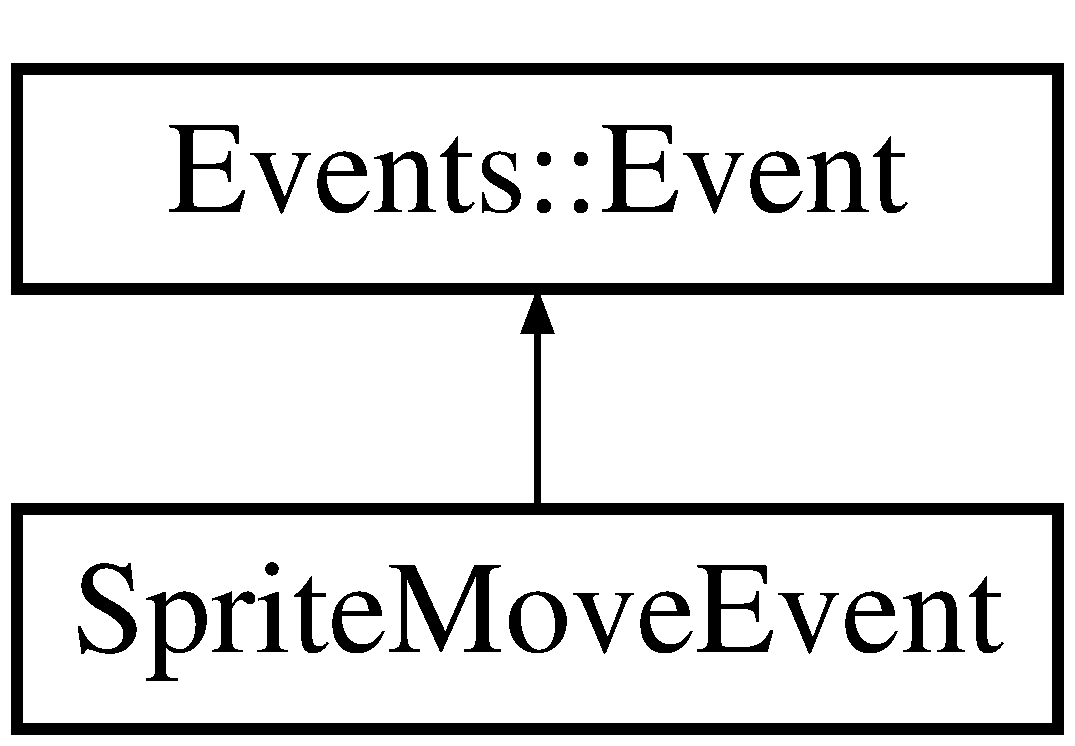
\includegraphics[height=2.000000cm]{class_sprite_move_event}
\end{center}
\end{figure}
\subsection*{Public Member Functions}
\begin{DoxyCompactItemize}
\item 
\hyperlink{class_sprite_move_event_af6f93f4fbedec36476948d5df7e15893}{Sprite\+Move\+Event} (const glm\+::vec2 \&\hyperlink{class_sprite_move_event_abf71a5443922204d31f96c14c1bc4dc0}{velocity}, const glm\+::vec2 \&\hyperlink{class_sprite_move_event_ad78a204593fa7266b54757758930606a}{next\+\_\+position})
\item 
const glm\+::vec2 \hyperlink{class_sprite_move_event_a8976431305e829b657d997ff3079aa15}{get\+Velocity} () const noexcept
\item 
const glm\+::vec2 \hyperlink{class_sprite_move_event_acd7f74b4dc39ce21f47395ef5fdb96e8}{get\+Next\+Position} () const noexcept
\end{DoxyCompactItemize}
\subsection*{Private Attributes}
\begin{DoxyCompactItemize}
\item 
glm\+::vec2 \hyperlink{class_sprite_move_event_abf71a5443922204d31f96c14c1bc4dc0}{velocity}
\item 
glm\+::vec2 \hyperlink{class_sprite_move_event_ad78a204593fa7266b54757758930606a}{next\+\_\+position}
\end{DoxyCompactItemize}


\subsection{Constructor \& Destructor Documentation}
\hypertarget{class_sprite_move_event_af6f93f4fbedec36476948d5df7e15893}{}\index{Sprite\+Move\+Event@{Sprite\+Move\+Event}!Sprite\+Move\+Event@{Sprite\+Move\+Event}}
\index{Sprite\+Move\+Event@{Sprite\+Move\+Event}!Sprite\+Move\+Event@{Sprite\+Move\+Event}}
\subsubsection[{Sprite\+Move\+Event}]{\setlength{\rightskip}{0pt plus 5cm}Sprite\+Move\+Event\+::\+Sprite\+Move\+Event (
\begin{DoxyParamCaption}
\item[{const glm\+::vec2 \&}]{velocity, }
\item[{const glm\+::vec2 \&}]{next\+\_\+position}
\end{DoxyParamCaption}
)\hspace{0.3cm}{\ttfamily [inline]}}\label{class_sprite_move_event_af6f93f4fbedec36476948d5df7e15893}


\subsection{Member Function Documentation}
\hypertarget{class_sprite_move_event_acd7f74b4dc39ce21f47395ef5fdb96e8}{}\index{Sprite\+Move\+Event@{Sprite\+Move\+Event}!get\+Next\+Position@{get\+Next\+Position}}
\index{get\+Next\+Position@{get\+Next\+Position}!Sprite\+Move\+Event@{Sprite\+Move\+Event}}
\subsubsection[{get\+Next\+Position}]{\setlength{\rightskip}{0pt plus 5cm}const glm\+::vec2 Sprite\+Move\+Event\+::get\+Next\+Position (
\begin{DoxyParamCaption}
{}
\end{DoxyParamCaption}
) const\hspace{0.3cm}{\ttfamily [inline]}, {\ttfamily [noexcept]}}\label{class_sprite_move_event_acd7f74b4dc39ce21f47395ef5fdb96e8}
\hypertarget{class_sprite_move_event_a8976431305e829b657d997ff3079aa15}{}\index{Sprite\+Move\+Event@{Sprite\+Move\+Event}!get\+Velocity@{get\+Velocity}}
\index{get\+Velocity@{get\+Velocity}!Sprite\+Move\+Event@{Sprite\+Move\+Event}}
\subsubsection[{get\+Velocity}]{\setlength{\rightskip}{0pt plus 5cm}const glm\+::vec2 Sprite\+Move\+Event\+::get\+Velocity (
\begin{DoxyParamCaption}
{}
\end{DoxyParamCaption}
) const\hspace{0.3cm}{\ttfamily [inline]}, {\ttfamily [noexcept]}}\label{class_sprite_move_event_a8976431305e829b657d997ff3079aa15}


\subsection{Member Data Documentation}
\hypertarget{class_sprite_move_event_ad78a204593fa7266b54757758930606a}{}\index{Sprite\+Move\+Event@{Sprite\+Move\+Event}!next\+\_\+position@{next\+\_\+position}}
\index{next\+\_\+position@{next\+\_\+position}!Sprite\+Move\+Event@{Sprite\+Move\+Event}}
\subsubsection[{next\+\_\+position}]{\setlength{\rightskip}{0pt plus 5cm}glm\+::vec2 Sprite\+Move\+Event\+::next\+\_\+position\hspace{0.3cm}{\ttfamily [private]}}\label{class_sprite_move_event_ad78a204593fa7266b54757758930606a}
\hypertarget{class_sprite_move_event_abf71a5443922204d31f96c14c1bc4dc0}{}\index{Sprite\+Move\+Event@{Sprite\+Move\+Event}!velocity@{velocity}}
\index{velocity@{velocity}!Sprite\+Move\+Event@{Sprite\+Move\+Event}}
\subsubsection[{velocity}]{\setlength{\rightskip}{0pt plus 5cm}glm\+::vec2 Sprite\+Move\+Event\+::velocity\hspace{0.3cm}{\ttfamily [private]}}\label{class_sprite_move_event_abf71a5443922204d31f96c14c1bc4dc0}


The documentation for this class was generated from the following file\+:\begin{DoxyCompactItemize}
\item 
src/\hyperlink{sprite__move__event_8h}{sprite\+\_\+move\+\_\+event.\+h}\end{DoxyCompactItemize}

\hypertarget{class_events_1_1_subject}{}\section{Events\+:\+:Subject Class Reference}
\label{class_events_1_1_subject}\index{Events\+::\+Subject@{Events\+::\+Subject}}


{\ttfamily \#include $<$subject.\+h$>$}

Inheritance diagram for Events\+:\+:Subject\+:\begin{figure}[H]
\begin{center}
\leavevmode
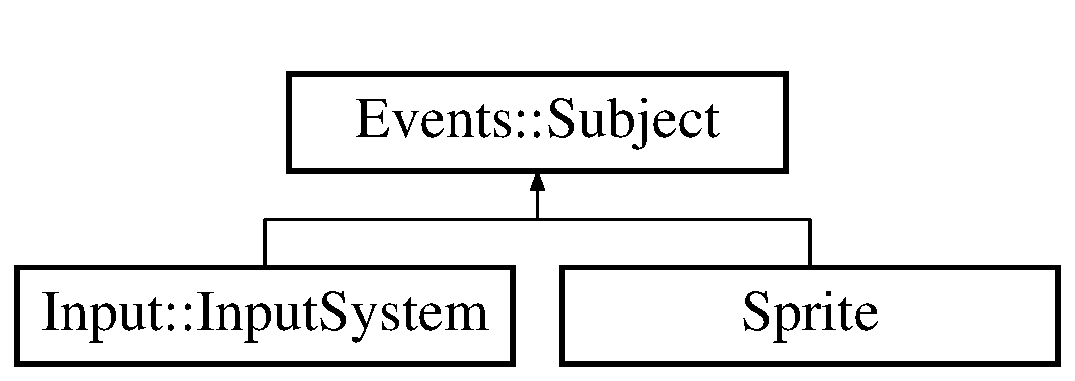
\includegraphics[height=2.000000cm]{class_events_1_1_subject}
\end{center}
\end{figure}
\subsection*{Public Member Functions}
\begin{DoxyCompactItemize}
\item 
void \hyperlink{class_events_1_1_subject_a9cf441c596a14b74a293412530052a56}{add\+Observer} (std\+::shared\+\_\+ptr$<$ \hyperlink{class_events_1_1_observer}{Observer} $>$ observer)
\item 
void \hyperlink{class_events_1_1_subject_a7b1c766879ff3687012a7262d551da4f}{remove\+Observer} (std\+::shared\+\_\+ptr$<$ \hyperlink{class_events_1_1_observer}{Observer} $>$ observer)
\end{DoxyCompactItemize}
\subsection*{Protected Member Functions}
\begin{DoxyCompactItemize}
\item 
void \hyperlink{class_events_1_1_subject_a7a9db96975d15deb897c4a53d0ff0dd3}{notify} (const \hyperlink{class_events_1_1_event}{Events\+::\+Event} \&event)
\end{DoxyCompactItemize}
\subsection*{Private Attributes}
\begin{DoxyCompactItemize}
\item 
std\+::list$<$ std\+::shared\+\_\+ptr$<$ \hyperlink{class_events_1_1_observer}{Observer} $>$ $>$ \hyperlink{class_events_1_1_subject_ad3018a440e8f470384c8543412ed5c22}{observers}
\end{DoxyCompactItemize}


\subsection{Member Function Documentation}
\hypertarget{class_events_1_1_subject_a9cf441c596a14b74a293412530052a56}{}\index{Events\+::\+Subject@{Events\+::\+Subject}!add\+Observer@{add\+Observer}}
\index{add\+Observer@{add\+Observer}!Events\+::\+Subject@{Events\+::\+Subject}}
\subsubsection[{add\+Observer}]{\setlength{\rightskip}{0pt plus 5cm}void Events\+::\+Subject\+::add\+Observer (
\begin{DoxyParamCaption}
\item[{std\+::shared\+\_\+ptr$<$ {\bf Observer} $>$}]{observer}
\end{DoxyParamCaption}
)}\label{class_events_1_1_subject_a9cf441c596a14b74a293412530052a56}
\hypertarget{class_events_1_1_subject_a7a9db96975d15deb897c4a53d0ff0dd3}{}\index{Events\+::\+Subject@{Events\+::\+Subject}!notify@{notify}}
\index{notify@{notify}!Events\+::\+Subject@{Events\+::\+Subject}}
\subsubsection[{notify}]{\setlength{\rightskip}{0pt plus 5cm}void Events\+::\+Subject\+::notify (
\begin{DoxyParamCaption}
\item[{const {\bf Events\+::\+Event} \&}]{event}
\end{DoxyParamCaption}
)\hspace{0.3cm}{\ttfamily [protected]}}\label{class_events_1_1_subject_a7a9db96975d15deb897c4a53d0ff0dd3}
\hypertarget{class_events_1_1_subject_a7b1c766879ff3687012a7262d551da4f}{}\index{Events\+::\+Subject@{Events\+::\+Subject}!remove\+Observer@{remove\+Observer}}
\index{remove\+Observer@{remove\+Observer}!Events\+::\+Subject@{Events\+::\+Subject}}
\subsubsection[{remove\+Observer}]{\setlength{\rightskip}{0pt plus 5cm}void Events\+::\+Subject\+::remove\+Observer (
\begin{DoxyParamCaption}
\item[{std\+::shared\+\_\+ptr$<$ {\bf Observer} $>$}]{observer}
\end{DoxyParamCaption}
)}\label{class_events_1_1_subject_a7b1c766879ff3687012a7262d551da4f}


\subsection{Member Data Documentation}
\hypertarget{class_events_1_1_subject_ad3018a440e8f470384c8543412ed5c22}{}\index{Events\+::\+Subject@{Events\+::\+Subject}!observers@{observers}}
\index{observers@{observers}!Events\+::\+Subject@{Events\+::\+Subject}}
\subsubsection[{observers}]{\setlength{\rightskip}{0pt plus 5cm}std\+::list$<$std\+::shared\+\_\+ptr$<${\bf Observer}$>$ $>$ Events\+::\+Subject\+::observers\hspace{0.3cm}{\ttfamily [private]}}\label{class_events_1_1_subject_ad3018a440e8f470384c8543412ed5c22}


The documentation for this class was generated from the following files\+:\begin{DoxyCompactItemize}
\item 
src/events/\hyperlink{subject_8h}{subject.\+h}\item 
src/events/\hyperlink{subject_8cpp}{subject.\+cpp}\end{DoxyCompactItemize}

\hypertarget{class_exceptions_1_1_system_already_initialized_exception}{}\section{Exceptions\+:\+:System\+Already\+Initialized\+Exception Class Reference}
\label{class_exceptions_1_1_system_already_initialized_exception}\index{Exceptions\+::\+System\+Already\+Initialized\+Exception@{Exceptions\+::\+System\+Already\+Initialized\+Exception}}


{\ttfamily \#include $<$system\+\_\+already\+\_\+initialized\+\_\+exception.\+h$>$}

Inheritance diagram for Exceptions\+:\+:System\+Already\+Initialized\+Exception\+:\begin{figure}[H]
\begin{center}
\leavevmode
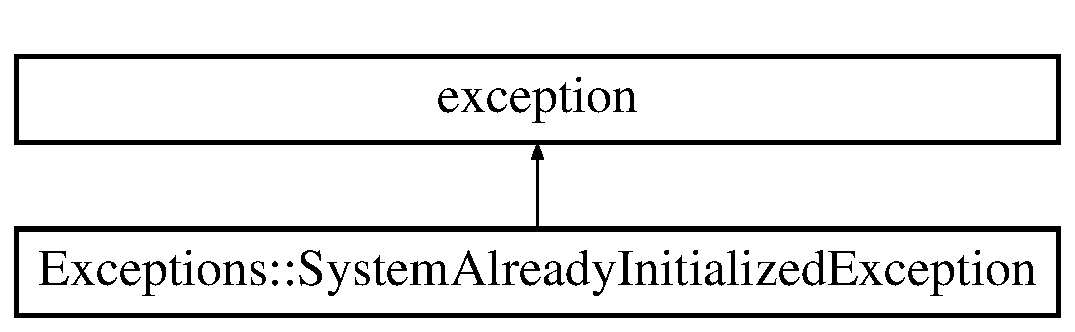
\includegraphics[height=2.000000cm]{class_exceptions_1_1_system_already_initialized_exception}
\end{center}
\end{figure}
\subsection*{Public Member Functions}
\begin{DoxyCompactItemize}
\item 
\hyperlink{class_exceptions_1_1_system_already_initialized_exception_a2f92ee1627417086ca29f3d58a8be520}{System\+Already\+Initialized\+Exception} (std\+::string \hyperlink{class_exceptions_1_1_system_already_initialized_exception_a858d81e072cf8a6a06a4fa506700fb32}{system\+\_\+name})
\item 
virtual const char $\ast$ \hyperlink{class_exceptions_1_1_system_already_initialized_exception_a28077450404b8dd5c89a348bc19ffa19}{what} () const   throw ()
\end{DoxyCompactItemize}
\subsection*{Private Attributes}
\begin{DoxyCompactItemize}
\item 
std\+::string \hyperlink{class_exceptions_1_1_system_already_initialized_exception_a858d81e072cf8a6a06a4fa506700fb32}{system\+\_\+name}
\end{DoxyCompactItemize}


\subsection{Constructor \& Destructor Documentation}
\hypertarget{class_exceptions_1_1_system_already_initialized_exception_a2f92ee1627417086ca29f3d58a8be520}{}\index{Exceptions\+::\+System\+Already\+Initialized\+Exception@{Exceptions\+::\+System\+Already\+Initialized\+Exception}!System\+Already\+Initialized\+Exception@{System\+Already\+Initialized\+Exception}}
\index{System\+Already\+Initialized\+Exception@{System\+Already\+Initialized\+Exception}!Exceptions\+::\+System\+Already\+Initialized\+Exception@{Exceptions\+::\+System\+Already\+Initialized\+Exception}}
\subsubsection[{System\+Already\+Initialized\+Exception}]{\setlength{\rightskip}{0pt plus 5cm}Exceptions\+::\+System\+Already\+Initialized\+Exception\+::\+System\+Already\+Initialized\+Exception (
\begin{DoxyParamCaption}
\item[{std\+::string}]{system\+\_\+name}
\end{DoxyParamCaption}
)\hspace{0.3cm}{\ttfamily [inline]}}\label{class_exceptions_1_1_system_already_initialized_exception_a2f92ee1627417086ca29f3d58a8be520}


\subsection{Member Function Documentation}
\hypertarget{class_exceptions_1_1_system_already_initialized_exception_a28077450404b8dd5c89a348bc19ffa19}{}\index{Exceptions\+::\+System\+Already\+Initialized\+Exception@{Exceptions\+::\+System\+Already\+Initialized\+Exception}!what@{what}}
\index{what@{what}!Exceptions\+::\+System\+Already\+Initialized\+Exception@{Exceptions\+::\+System\+Already\+Initialized\+Exception}}
\subsubsection[{what}]{\setlength{\rightskip}{0pt plus 5cm}virtual const char$\ast$ Exceptions\+::\+System\+Already\+Initialized\+Exception\+::what (
\begin{DoxyParamCaption}
{}
\end{DoxyParamCaption}
) const throw  ) \hspace{0.3cm}{\ttfamily [inline]}, {\ttfamily [virtual]}}\label{class_exceptions_1_1_system_already_initialized_exception_a28077450404b8dd5c89a348bc19ffa19}


\subsection{Member Data Documentation}
\hypertarget{class_exceptions_1_1_system_already_initialized_exception_a858d81e072cf8a6a06a4fa506700fb32}{}\index{Exceptions\+::\+System\+Already\+Initialized\+Exception@{Exceptions\+::\+System\+Already\+Initialized\+Exception}!system\+\_\+name@{system\+\_\+name}}
\index{system\+\_\+name@{system\+\_\+name}!Exceptions\+::\+System\+Already\+Initialized\+Exception@{Exceptions\+::\+System\+Already\+Initialized\+Exception}}
\subsubsection[{system\+\_\+name}]{\setlength{\rightskip}{0pt plus 5cm}std\+::string Exceptions\+::\+System\+Already\+Initialized\+Exception\+::system\+\_\+name\hspace{0.3cm}{\ttfamily [private]}}\label{class_exceptions_1_1_system_already_initialized_exception_a858d81e072cf8a6a06a4fa506700fb32}


The documentation for this class was generated from the following file\+:\begin{DoxyCompactItemize}
\item 
src/exceptions/\hyperlink{system__already__initialized__exception_8h}{system\+\_\+already\+\_\+initialized\+\_\+exception.\+h}\end{DoxyCompactItemize}

\hypertarget{class_exceptions_1_1_system_already_running_exception}{}\section{Exceptions\+:\+:System\+Already\+Running\+Exception Class Reference}
\label{class_exceptions_1_1_system_already_running_exception}\index{Exceptions\+::\+System\+Already\+Running\+Exception@{Exceptions\+::\+System\+Already\+Running\+Exception}}


{\ttfamily \#include $<$system\+\_\+already\+\_\+running\+\_\+exception.\+h$>$}

Inheritance diagram for Exceptions\+:\+:System\+Already\+Running\+Exception\+:\begin{figure}[H]
\begin{center}
\leavevmode
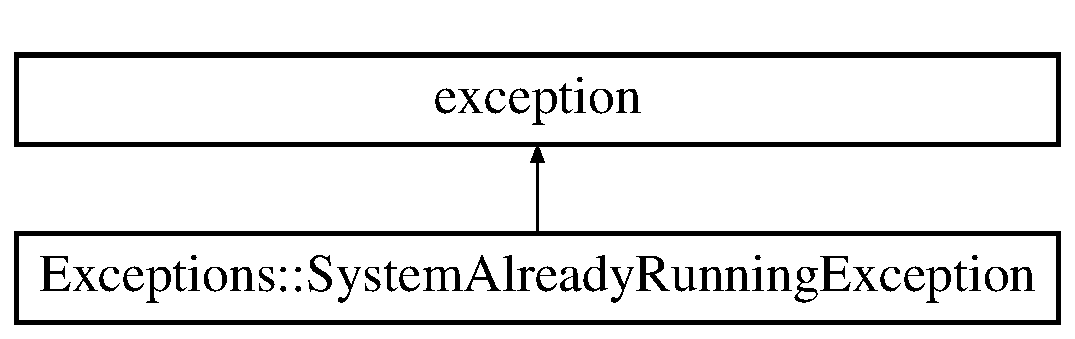
\includegraphics[height=2.000000cm]{class_exceptions_1_1_system_already_running_exception}
\end{center}
\end{figure}
\subsection*{Public Member Functions}
\begin{DoxyCompactItemize}
\item 
\hyperlink{class_exceptions_1_1_system_already_running_exception_aed8f9f444543924acea118e7485fdbba}{System\+Already\+Running\+Exception} (std\+::string \hyperlink{class_exceptions_1_1_system_already_running_exception_a914a5cb77c9acbd05862c8927da7ea36}{system\+\_\+name})
\item 
virtual const char $\ast$ \hyperlink{class_exceptions_1_1_system_already_running_exception_a558ddbeefc7c578b0a2c7ac031a5aef5}{what} () const   throw ()
\end{DoxyCompactItemize}
\subsection*{Private Attributes}
\begin{DoxyCompactItemize}
\item 
std\+::string \hyperlink{class_exceptions_1_1_system_already_running_exception_a914a5cb77c9acbd05862c8927da7ea36}{system\+\_\+name}
\end{DoxyCompactItemize}


\subsection{Constructor \& Destructor Documentation}
\hypertarget{class_exceptions_1_1_system_already_running_exception_aed8f9f444543924acea118e7485fdbba}{}\index{Exceptions\+::\+System\+Already\+Running\+Exception@{Exceptions\+::\+System\+Already\+Running\+Exception}!System\+Already\+Running\+Exception@{System\+Already\+Running\+Exception}}
\index{System\+Already\+Running\+Exception@{System\+Already\+Running\+Exception}!Exceptions\+::\+System\+Already\+Running\+Exception@{Exceptions\+::\+System\+Already\+Running\+Exception}}
\subsubsection[{System\+Already\+Running\+Exception}]{\setlength{\rightskip}{0pt plus 5cm}Exceptions\+::\+System\+Already\+Running\+Exception\+::\+System\+Already\+Running\+Exception (
\begin{DoxyParamCaption}
\item[{std\+::string}]{system\+\_\+name}
\end{DoxyParamCaption}
)\hspace{0.3cm}{\ttfamily [inline]}}\label{class_exceptions_1_1_system_already_running_exception_aed8f9f444543924acea118e7485fdbba}


\subsection{Member Function Documentation}
\hypertarget{class_exceptions_1_1_system_already_running_exception_a558ddbeefc7c578b0a2c7ac031a5aef5}{}\index{Exceptions\+::\+System\+Already\+Running\+Exception@{Exceptions\+::\+System\+Already\+Running\+Exception}!what@{what}}
\index{what@{what}!Exceptions\+::\+System\+Already\+Running\+Exception@{Exceptions\+::\+System\+Already\+Running\+Exception}}
\subsubsection[{what}]{\setlength{\rightskip}{0pt plus 5cm}virtual const char$\ast$ Exceptions\+::\+System\+Already\+Running\+Exception\+::what (
\begin{DoxyParamCaption}
{}
\end{DoxyParamCaption}
) const throw  ) \hspace{0.3cm}{\ttfamily [inline]}, {\ttfamily [virtual]}}\label{class_exceptions_1_1_system_already_running_exception_a558ddbeefc7c578b0a2c7ac031a5aef5}


\subsection{Member Data Documentation}
\hypertarget{class_exceptions_1_1_system_already_running_exception_a914a5cb77c9acbd05862c8927da7ea36}{}\index{Exceptions\+::\+System\+Already\+Running\+Exception@{Exceptions\+::\+System\+Already\+Running\+Exception}!system\+\_\+name@{system\+\_\+name}}
\index{system\+\_\+name@{system\+\_\+name}!Exceptions\+::\+System\+Already\+Running\+Exception@{Exceptions\+::\+System\+Already\+Running\+Exception}}
\subsubsection[{system\+\_\+name}]{\setlength{\rightskip}{0pt plus 5cm}std\+::string Exceptions\+::\+System\+Already\+Running\+Exception\+::system\+\_\+name\hspace{0.3cm}{\ttfamily [private]}}\label{class_exceptions_1_1_system_already_running_exception_a914a5cb77c9acbd05862c8927da7ea36}


The documentation for this class was generated from the following file\+:\begin{DoxyCompactItemize}
\item 
src/exceptions/\hyperlink{system__already__running__exception_8h}{system\+\_\+already\+\_\+running\+\_\+exception.\+h}\end{DoxyCompactItemize}

\hypertarget{class_exceptions_1_1_system_not_initialized_exception}{}\section{Exceptions\+:\+:System\+Not\+Initialized\+Exception Class Reference}
\label{class_exceptions_1_1_system_not_initialized_exception}\index{Exceptions\+::\+System\+Not\+Initialized\+Exception@{Exceptions\+::\+System\+Not\+Initialized\+Exception}}


{\ttfamily \#include $<$system\+\_\+not\+\_\+initialized\+\_\+exception.\+h$>$}

Inheritance diagram for Exceptions\+:\+:System\+Not\+Initialized\+Exception\+:\begin{figure}[H]
\begin{center}
\leavevmode
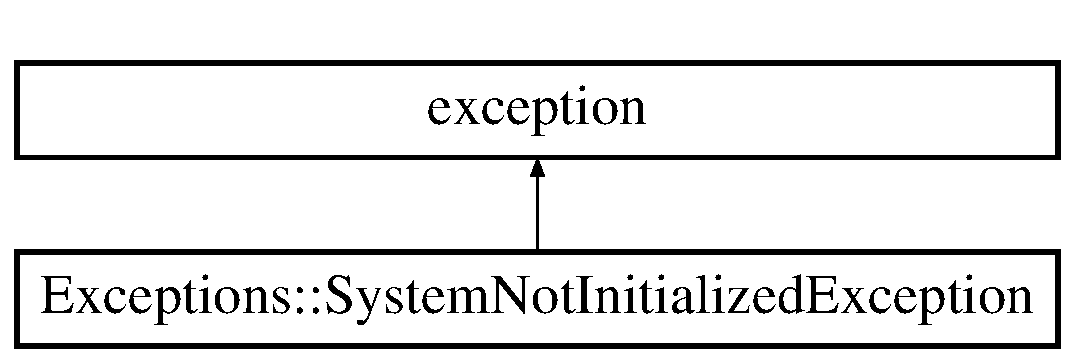
\includegraphics[height=2.000000cm]{class_exceptions_1_1_system_not_initialized_exception}
\end{center}
\end{figure}
\subsection*{Public Member Functions}
\begin{DoxyCompactItemize}
\item 
\hyperlink{class_exceptions_1_1_system_not_initialized_exception_ac22625946ad8f784f8c78b1b5b2970d7}{System\+Not\+Initialized\+Exception} (std\+::string \hyperlink{class_exceptions_1_1_system_not_initialized_exception_a5649bbb869394d52f7c8aa82d600d070}{system\+\_\+name})
\item 
virtual const char $\ast$ \hyperlink{class_exceptions_1_1_system_not_initialized_exception_a6481e3f2f2dd245e47ed246b12ce61c5}{what} () const   throw ()
\end{DoxyCompactItemize}
\subsection*{Private Attributes}
\begin{DoxyCompactItemize}
\item 
std\+::string \hyperlink{class_exceptions_1_1_system_not_initialized_exception_a5649bbb869394d52f7c8aa82d600d070}{system\+\_\+name}
\end{DoxyCompactItemize}


\subsection{Constructor \& Destructor Documentation}
\hypertarget{class_exceptions_1_1_system_not_initialized_exception_ac22625946ad8f784f8c78b1b5b2970d7}{}\index{Exceptions\+::\+System\+Not\+Initialized\+Exception@{Exceptions\+::\+System\+Not\+Initialized\+Exception}!System\+Not\+Initialized\+Exception@{System\+Not\+Initialized\+Exception}}
\index{System\+Not\+Initialized\+Exception@{System\+Not\+Initialized\+Exception}!Exceptions\+::\+System\+Not\+Initialized\+Exception@{Exceptions\+::\+System\+Not\+Initialized\+Exception}}
\subsubsection[{System\+Not\+Initialized\+Exception}]{\setlength{\rightskip}{0pt plus 5cm}Exceptions\+::\+System\+Not\+Initialized\+Exception\+::\+System\+Not\+Initialized\+Exception (
\begin{DoxyParamCaption}
\item[{std\+::string}]{system\+\_\+name}
\end{DoxyParamCaption}
)\hspace{0.3cm}{\ttfamily [inline]}}\label{class_exceptions_1_1_system_not_initialized_exception_ac22625946ad8f784f8c78b1b5b2970d7}


\subsection{Member Function Documentation}
\hypertarget{class_exceptions_1_1_system_not_initialized_exception_a6481e3f2f2dd245e47ed246b12ce61c5}{}\index{Exceptions\+::\+System\+Not\+Initialized\+Exception@{Exceptions\+::\+System\+Not\+Initialized\+Exception}!what@{what}}
\index{what@{what}!Exceptions\+::\+System\+Not\+Initialized\+Exception@{Exceptions\+::\+System\+Not\+Initialized\+Exception}}
\subsubsection[{what}]{\setlength{\rightskip}{0pt plus 5cm}virtual const char$\ast$ Exceptions\+::\+System\+Not\+Initialized\+Exception\+::what (
\begin{DoxyParamCaption}
{}
\end{DoxyParamCaption}
) const throw  ) \hspace{0.3cm}{\ttfamily [inline]}, {\ttfamily [virtual]}}\label{class_exceptions_1_1_system_not_initialized_exception_a6481e3f2f2dd245e47ed246b12ce61c5}


\subsection{Member Data Documentation}
\hypertarget{class_exceptions_1_1_system_not_initialized_exception_a5649bbb869394d52f7c8aa82d600d070}{}\index{Exceptions\+::\+System\+Not\+Initialized\+Exception@{Exceptions\+::\+System\+Not\+Initialized\+Exception}!system\+\_\+name@{system\+\_\+name}}
\index{system\+\_\+name@{system\+\_\+name}!Exceptions\+::\+System\+Not\+Initialized\+Exception@{Exceptions\+::\+System\+Not\+Initialized\+Exception}}
\subsubsection[{system\+\_\+name}]{\setlength{\rightskip}{0pt plus 5cm}std\+::string Exceptions\+::\+System\+Not\+Initialized\+Exception\+::system\+\_\+name\hspace{0.3cm}{\ttfamily [private]}}\label{class_exceptions_1_1_system_not_initialized_exception_a5649bbb869394d52f7c8aa82d600d070}


The documentation for this class was generated from the following file\+:\begin{DoxyCompactItemize}
\item 
src/exceptions/\hyperlink{system__not__initialized__exception_8h}{system\+\_\+not\+\_\+initialized\+\_\+exception.\+h}\end{DoxyCompactItemize}

\hypertarget{class_exceptions_1_1_system_not_running_exception}{}\section{Exceptions\+:\+:System\+Not\+Running\+Exception Class Reference}
\label{class_exceptions_1_1_system_not_running_exception}\index{Exceptions\+::\+System\+Not\+Running\+Exception@{Exceptions\+::\+System\+Not\+Running\+Exception}}


{\ttfamily \#include $<$system\+\_\+not\+\_\+running\+\_\+exception.\+h$>$}

Inheritance diagram for Exceptions\+:\+:System\+Not\+Running\+Exception\+:\begin{figure}[H]
\begin{center}
\leavevmode
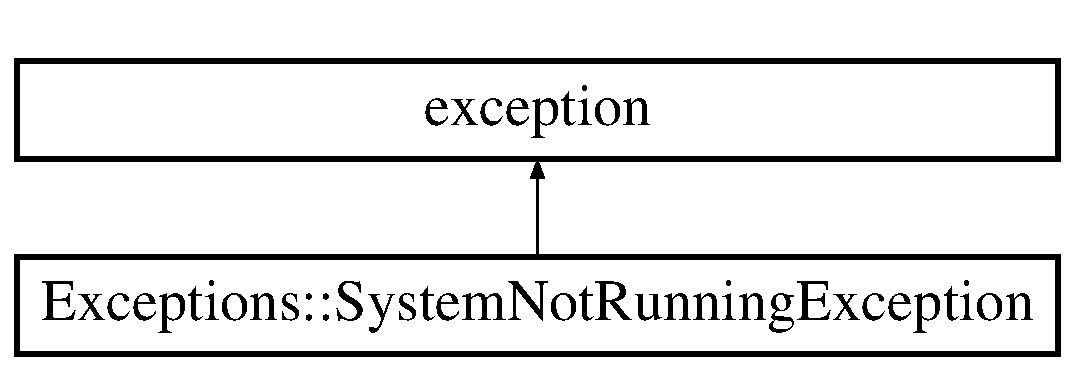
\includegraphics[height=2.000000cm]{class_exceptions_1_1_system_not_running_exception}
\end{center}
\end{figure}
\subsection*{Public Member Functions}
\begin{DoxyCompactItemize}
\item 
\hyperlink{class_exceptions_1_1_system_not_running_exception_aed32e775ba2eb68ff70446c138c40bcc}{System\+Not\+Running\+Exception} (std\+::string \hyperlink{class_exceptions_1_1_system_not_running_exception_af97cd0ba9e5c5b4aa57b99028b6bb95a}{system\+\_\+name})
\item 
virtual const char $\ast$ \hyperlink{class_exceptions_1_1_system_not_running_exception_afc7a24ce91303377321104405996f5ff}{what} () const   throw ()
\end{DoxyCompactItemize}
\subsection*{Private Attributes}
\begin{DoxyCompactItemize}
\item 
std\+::string \hyperlink{class_exceptions_1_1_system_not_running_exception_af97cd0ba9e5c5b4aa57b99028b6bb95a}{system\+\_\+name}
\end{DoxyCompactItemize}


\subsection{Constructor \& Destructor Documentation}
\hypertarget{class_exceptions_1_1_system_not_running_exception_aed32e775ba2eb68ff70446c138c40bcc}{}\index{Exceptions\+::\+System\+Not\+Running\+Exception@{Exceptions\+::\+System\+Not\+Running\+Exception}!System\+Not\+Running\+Exception@{System\+Not\+Running\+Exception}}
\index{System\+Not\+Running\+Exception@{System\+Not\+Running\+Exception}!Exceptions\+::\+System\+Not\+Running\+Exception@{Exceptions\+::\+System\+Not\+Running\+Exception}}
\subsubsection[{System\+Not\+Running\+Exception}]{\setlength{\rightskip}{0pt plus 5cm}Exceptions\+::\+System\+Not\+Running\+Exception\+::\+System\+Not\+Running\+Exception (
\begin{DoxyParamCaption}
\item[{std\+::string}]{system\+\_\+name}
\end{DoxyParamCaption}
)\hspace{0.3cm}{\ttfamily [inline]}}\label{class_exceptions_1_1_system_not_running_exception_aed32e775ba2eb68ff70446c138c40bcc}


\subsection{Member Function Documentation}
\hypertarget{class_exceptions_1_1_system_not_running_exception_afc7a24ce91303377321104405996f5ff}{}\index{Exceptions\+::\+System\+Not\+Running\+Exception@{Exceptions\+::\+System\+Not\+Running\+Exception}!what@{what}}
\index{what@{what}!Exceptions\+::\+System\+Not\+Running\+Exception@{Exceptions\+::\+System\+Not\+Running\+Exception}}
\subsubsection[{what}]{\setlength{\rightskip}{0pt plus 5cm}virtual const char$\ast$ Exceptions\+::\+System\+Not\+Running\+Exception\+::what (
\begin{DoxyParamCaption}
{}
\end{DoxyParamCaption}
) const throw  ) \hspace{0.3cm}{\ttfamily [inline]}, {\ttfamily [virtual]}}\label{class_exceptions_1_1_system_not_running_exception_afc7a24ce91303377321104405996f5ff}


\subsection{Member Data Documentation}
\hypertarget{class_exceptions_1_1_system_not_running_exception_af97cd0ba9e5c5b4aa57b99028b6bb95a}{}\index{Exceptions\+::\+System\+Not\+Running\+Exception@{Exceptions\+::\+System\+Not\+Running\+Exception}!system\+\_\+name@{system\+\_\+name}}
\index{system\+\_\+name@{system\+\_\+name}!Exceptions\+::\+System\+Not\+Running\+Exception@{Exceptions\+::\+System\+Not\+Running\+Exception}}
\subsubsection[{system\+\_\+name}]{\setlength{\rightskip}{0pt plus 5cm}std\+::string Exceptions\+::\+System\+Not\+Running\+Exception\+::system\+\_\+name\hspace{0.3cm}{\ttfamily [private]}}\label{class_exceptions_1_1_system_not_running_exception_af97cd0ba9e5c5b4aa57b99028b6bb95a}


The documentation for this class was generated from the following file\+:\begin{DoxyCompactItemize}
\item 
src/exceptions/\hyperlink{system__not__running__exception_8h}{system\+\_\+not\+\_\+running\+\_\+exception.\+h}\end{DoxyCompactItemize}

\hypertarget{class_test_attribute_trait}{}\section{Test\+Attribute\+Trait Class Reference}
\label{class_test_attribute_trait}\index{Test\+Attribute\+Trait@{Test\+Attribute\+Trait}}
Inheritance diagram for Test\+Attribute\+Trait\+:\begin{figure}[H]
\begin{center}
\leavevmode
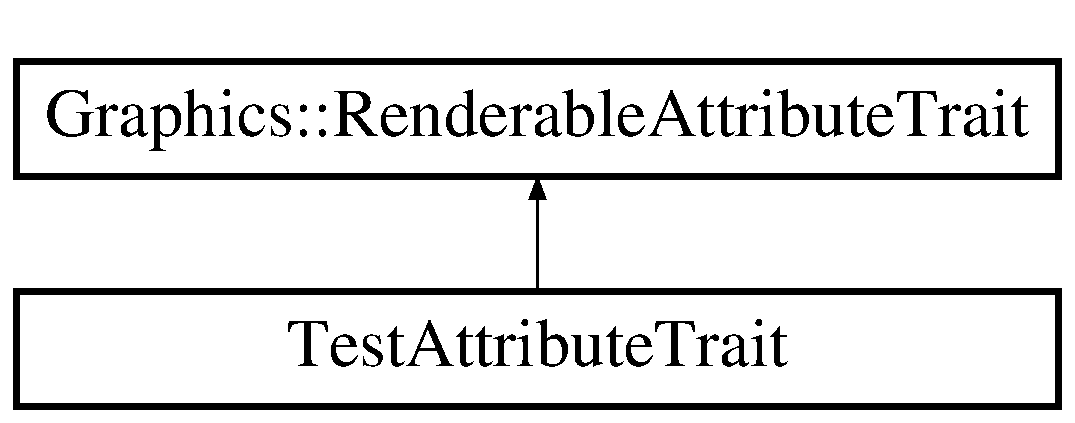
\includegraphics[height=3.000000cm]{class_test_attribute_trait}
\end{center}
\end{figure}
\subsection*{Public Member Functions}
\begin{DoxyCompactItemize}
\item 
\hyperlink{class_test_attribute_trait_abf91ded2bc981ff07f82f5808291aa27}{Test\+Attribute\+Trait} ()
\item 
virtual const std\+::map$<$ \hyperlink{class_graphics_1_1_vertex_data_a50e88236939dc2a3ec4df7aeb728620e}{Graphics\+::\+Vertex\+Data\+::\+D\+A\+T\+A\+\_\+\+T\+Y\+P\+E}, unsigned int $>$ \hyperlink{class_test_attribute_trait_af121ef5fbd5bcda4bbbc7fdadd5599c8}{operator()} () const noexceptoverride
\end{DoxyCompactItemize}
\subsection*{Private Attributes}
\begin{DoxyCompactItemize}
\item 
std\+::map$<$ \hyperlink{class_graphics_1_1_vertex_data_a50e88236939dc2a3ec4df7aeb728620e}{Graphics\+::\+Vertex\+Data\+::\+D\+A\+T\+A\+\_\+\+T\+Y\+P\+E}, unsigned int $>$ \hyperlink{class_test_attribute_trait_a4e8fa71f7e6ced6e221c08a5a19a46a5}{trait}
\end{DoxyCompactItemize}


\subsection{Constructor \& Destructor Documentation}
\hypertarget{class_test_attribute_trait_abf91ded2bc981ff07f82f5808291aa27}{}\index{Test\+Attribute\+Trait@{Test\+Attribute\+Trait}!Test\+Attribute\+Trait@{Test\+Attribute\+Trait}}
\index{Test\+Attribute\+Trait@{Test\+Attribute\+Trait}!Test\+Attribute\+Trait@{Test\+Attribute\+Trait}}
\subsubsection[{Test\+Attribute\+Trait}]{\setlength{\rightskip}{0pt plus 5cm}Test\+Attribute\+Trait\+::\+Test\+Attribute\+Trait (
\begin{DoxyParamCaption}
{}
\end{DoxyParamCaption}
)\hspace{0.3cm}{\ttfamily [inline]}}\label{class_test_attribute_trait_abf91ded2bc981ff07f82f5808291aa27}


\subsection{Member Function Documentation}
\hypertarget{class_test_attribute_trait_af121ef5fbd5bcda4bbbc7fdadd5599c8}{}\index{Test\+Attribute\+Trait@{Test\+Attribute\+Trait}!operator()@{operator()}}
\index{operator()@{operator()}!Test\+Attribute\+Trait@{Test\+Attribute\+Trait}}
\subsubsection[{operator()}]{\setlength{\rightskip}{0pt plus 5cm}virtual const std\+::map$<${\bf Graphics\+::\+Vertex\+Data\+::\+D\+A\+T\+A\+\_\+\+T\+Y\+P\+E}, unsigned int$>$ Test\+Attribute\+Trait\+::operator() (
\begin{DoxyParamCaption}
{}
\end{DoxyParamCaption}
) const\hspace{0.3cm}{\ttfamily [inline]}, {\ttfamily [override]}, {\ttfamily [virtual]}, {\ttfamily [noexcept]}}\label{class_test_attribute_trait_af121ef5fbd5bcda4bbbc7fdadd5599c8}


Reimplemented from \hyperlink{class_graphics_1_1_renderable_attribute_trait_a44401f624ace1dc71220e7064db92465}{Graphics\+::\+Renderable\+Attribute\+Trait}.



\subsection{Member Data Documentation}
\hypertarget{class_test_attribute_trait_a4e8fa71f7e6ced6e221c08a5a19a46a5}{}\index{Test\+Attribute\+Trait@{Test\+Attribute\+Trait}!trait@{trait}}
\index{trait@{trait}!Test\+Attribute\+Trait@{Test\+Attribute\+Trait}}
\subsubsection[{trait}]{\setlength{\rightskip}{0pt plus 5cm}std\+::map$<${\bf Graphics\+::\+Vertex\+Data\+::\+D\+A\+T\+A\+\_\+\+T\+Y\+P\+E}, unsigned int$>$ Test\+Attribute\+Trait\+::trait\hspace{0.3cm}{\ttfamily [private]}}\label{class_test_attribute_trait_a4e8fa71f7e6ced6e221c08a5a19a46a5}


The documentation for this class was generated from the following file\+:\begin{DoxyCompactItemize}
\item 
test/graphics/\hyperlink{renderable__test_8cpp}{renderable\+\_\+test.\+cpp}\end{DoxyCompactItemize}

\hypertarget{class_graphics_1_1_texture_manager}{}\section{Graphics\+:\+:Texture\+Manager Class Reference}
\label{class_graphics_1_1_texture_manager}\index{Graphics\+::\+Texture\+Manager@{Graphics\+::\+Texture\+Manager}}


{\ttfamily \#include $<$texture\+\_\+manager.\+h$>$}

\subsection*{Public Member Functions}
\begin{DoxyCompactItemize}
\item 
\hyperlink{class_graphics_1_1_texture_manager_aa04c4948f0bf5641454b649c8ddd8ebd}{Texture\+Manager} ()
\item 
\hyperlink{class_graphics_1_1_texture_manager_a37197d06634adca1715ce58a1d46a98f}{$\sim$\+Texture\+Manager} ()
\item 
const bool \hyperlink{class_graphics_1_1_texture_manager_aaf3f4c4eae602c748482950639335dee}{load\+Texture} (const std\+::string \&path, const std\+::string \&texture\+\_\+uniform\+\_\+name, const unsigned int texture\+\_\+unit=0)
\item 
const std\+::shared\+\_\+ptr$<$ \hyperlink{class_graphics_1_1_base_texture}{Base\+Texture} $>$ \hyperlink{class_graphics_1_1_texture_manager_ae2c15e90de3a93f02609f5da3a050e5c}{operator\mbox{[}$\,$\mbox{]}} (const std\+::string \&name) const 
\item 
const std\+::shared\+\_\+ptr$<$ \hyperlink{class_graphics_1_1_base_texture}{Base\+Texture} $>$ \hyperlink{class_graphics_1_1_texture_manager_a4e969b690676e3f5f764fa2a2c67763b}{get\+Texture} (const std\+::string \&name) const 
\item 
const bool \hyperlink{class_graphics_1_1_texture_manager_a7ea7b24ff436064895eece7804e4c18d}{texture\+Exists} (const std\+::string \&name) const noexcept
\end{DoxyCompactItemize}
\subsection*{Static Public Member Functions}
\begin{DoxyCompactItemize}
\item 
static const std\+::string \hyperlink{class_graphics_1_1_texture_manager_a5011ab2205d5dd2e4d0fcecbf91a00cc}{get\+Name\+From\+Path} (const std\+::string \&path) noexcept
\end{DoxyCompactItemize}
\subsection*{Private Attributes}
\begin{DoxyCompactItemize}
\item 
std\+::map$<$ std\+::string, std\+::shared\+\_\+ptr$<$ \hyperlink{class_graphics_1_1_base_texture}{Base\+Texture} $>$ $>$ \hyperlink{class_graphics_1_1_texture_manager_ac8e9f344711185e1d002b021041d137e}{textures\+\_\+to\+\_\+names}
\end{DoxyCompactItemize}


\subsection{Constructor \& Destructor Documentation}
\hypertarget{class_graphics_1_1_texture_manager_aa04c4948f0bf5641454b649c8ddd8ebd}{}\index{Graphics\+::\+Texture\+Manager@{Graphics\+::\+Texture\+Manager}!Texture\+Manager@{Texture\+Manager}}
\index{Texture\+Manager@{Texture\+Manager}!Graphics\+::\+Texture\+Manager@{Graphics\+::\+Texture\+Manager}}
\subsubsection[{Texture\+Manager}]{\setlength{\rightskip}{0pt plus 5cm}Graphics\+::\+Texture\+Manager\+::\+Texture\+Manager (
\begin{DoxyParamCaption}
{}
\end{DoxyParamCaption}
)}\label{class_graphics_1_1_texture_manager_aa04c4948f0bf5641454b649c8ddd8ebd}
\hypertarget{class_graphics_1_1_texture_manager_a37197d06634adca1715ce58a1d46a98f}{}\index{Graphics\+::\+Texture\+Manager@{Graphics\+::\+Texture\+Manager}!````~Texture\+Manager@{$\sim$\+Texture\+Manager}}
\index{````~Texture\+Manager@{$\sim$\+Texture\+Manager}!Graphics\+::\+Texture\+Manager@{Graphics\+::\+Texture\+Manager}}
\subsubsection[{$\sim$\+Texture\+Manager}]{\setlength{\rightskip}{0pt plus 5cm}Graphics\+::\+Texture\+Manager\+::$\sim$\+Texture\+Manager (
\begin{DoxyParamCaption}
{}
\end{DoxyParamCaption}
)}\label{class_graphics_1_1_texture_manager_a37197d06634adca1715ce58a1d46a98f}


\subsection{Member Function Documentation}
\hypertarget{class_graphics_1_1_texture_manager_a5011ab2205d5dd2e4d0fcecbf91a00cc}{}\index{Graphics\+::\+Texture\+Manager@{Graphics\+::\+Texture\+Manager}!get\+Name\+From\+Path@{get\+Name\+From\+Path}}
\index{get\+Name\+From\+Path@{get\+Name\+From\+Path}!Graphics\+::\+Texture\+Manager@{Graphics\+::\+Texture\+Manager}}
\subsubsection[{get\+Name\+From\+Path}]{\setlength{\rightskip}{0pt plus 5cm}const std\+::string Graphics\+::\+Texture\+Manager\+::get\+Name\+From\+Path (
\begin{DoxyParamCaption}
\item[{const std\+::string \&}]{path}
\end{DoxyParamCaption}
)\hspace{0.3cm}{\ttfamily [static]}, {\ttfamily [noexcept]}}\label{class_graphics_1_1_texture_manager_a5011ab2205d5dd2e4d0fcecbf91a00cc}
\hypertarget{class_graphics_1_1_texture_manager_a4e969b690676e3f5f764fa2a2c67763b}{}\index{Graphics\+::\+Texture\+Manager@{Graphics\+::\+Texture\+Manager}!get\+Texture@{get\+Texture}}
\index{get\+Texture@{get\+Texture}!Graphics\+::\+Texture\+Manager@{Graphics\+::\+Texture\+Manager}}
\subsubsection[{get\+Texture}]{\setlength{\rightskip}{0pt plus 5cm}const std\+::shared\+\_\+ptr$<$ {\bf Base\+Texture} $>$ Graphics\+::\+Texture\+Manager\+::get\+Texture (
\begin{DoxyParamCaption}
\item[{const std\+::string \&}]{name}
\end{DoxyParamCaption}
) const}\label{class_graphics_1_1_texture_manager_a4e969b690676e3f5f764fa2a2c67763b}
\hypertarget{class_graphics_1_1_texture_manager_aaf3f4c4eae602c748482950639335dee}{}\index{Graphics\+::\+Texture\+Manager@{Graphics\+::\+Texture\+Manager}!load\+Texture@{load\+Texture}}
\index{load\+Texture@{load\+Texture}!Graphics\+::\+Texture\+Manager@{Graphics\+::\+Texture\+Manager}}
\subsubsection[{load\+Texture}]{\setlength{\rightskip}{0pt plus 5cm}const bool Graphics\+::\+Texture\+Manager\+::load\+Texture (
\begin{DoxyParamCaption}
\item[{const std\+::string \&}]{path, }
\item[{const std\+::string \&}]{texture\+\_\+uniform\+\_\+name, }
\item[{const unsigned int}]{texture\+\_\+unit = {\ttfamily 0}}
\end{DoxyParamCaption}
)}\label{class_graphics_1_1_texture_manager_aaf3f4c4eae602c748482950639335dee}
\hypertarget{class_graphics_1_1_texture_manager_ae2c15e90de3a93f02609f5da3a050e5c}{}\index{Graphics\+::\+Texture\+Manager@{Graphics\+::\+Texture\+Manager}!operator\mbox{[}$\,$\mbox{]}@{operator[]}}
\index{operator\mbox{[}$\,$\mbox{]}@{operator[]}!Graphics\+::\+Texture\+Manager@{Graphics\+::\+Texture\+Manager}}
\subsubsection[{operator[]}]{\setlength{\rightskip}{0pt plus 5cm}const std\+::shared\+\_\+ptr$<$ {\bf Base\+Texture} $>$ Graphics\+::\+Texture\+Manager\+::operator\mbox{[}$\,$\mbox{]} (
\begin{DoxyParamCaption}
\item[{const std\+::string \&}]{name}
\end{DoxyParamCaption}
) const}\label{class_graphics_1_1_texture_manager_ae2c15e90de3a93f02609f5da3a050e5c}
\hypertarget{class_graphics_1_1_texture_manager_a7ea7b24ff436064895eece7804e4c18d}{}\index{Graphics\+::\+Texture\+Manager@{Graphics\+::\+Texture\+Manager}!texture\+Exists@{texture\+Exists}}
\index{texture\+Exists@{texture\+Exists}!Graphics\+::\+Texture\+Manager@{Graphics\+::\+Texture\+Manager}}
\subsubsection[{texture\+Exists}]{\setlength{\rightskip}{0pt plus 5cm}const bool Graphics\+::\+Texture\+Manager\+::texture\+Exists (
\begin{DoxyParamCaption}
\item[{const std\+::string \&}]{name}
\end{DoxyParamCaption}
) const\hspace{0.3cm}{\ttfamily [noexcept]}}\label{class_graphics_1_1_texture_manager_a7ea7b24ff436064895eece7804e4c18d}


\subsection{Member Data Documentation}
\hypertarget{class_graphics_1_1_texture_manager_ac8e9f344711185e1d002b021041d137e}{}\index{Graphics\+::\+Texture\+Manager@{Graphics\+::\+Texture\+Manager}!textures\+\_\+to\+\_\+names@{textures\+\_\+to\+\_\+names}}
\index{textures\+\_\+to\+\_\+names@{textures\+\_\+to\+\_\+names}!Graphics\+::\+Texture\+Manager@{Graphics\+::\+Texture\+Manager}}
\subsubsection[{textures\+\_\+to\+\_\+names}]{\setlength{\rightskip}{0pt plus 5cm}std\+::map$<$std\+::string, std\+::shared\+\_\+ptr$<${\bf Base\+Texture}$>$ $>$ Graphics\+::\+Texture\+Manager\+::textures\+\_\+to\+\_\+names\hspace{0.3cm}{\ttfamily [private]}}\label{class_graphics_1_1_texture_manager_ac8e9f344711185e1d002b021041d137e}


The documentation for this class was generated from the following files\+:\begin{DoxyCompactItemize}
\item 
src/graphics/\hyperlink{texture__manager_8h}{texture\+\_\+manager.\+h}\item 
src/graphics/\hyperlink{texture__manager_8cpp}{texture\+\_\+manager.\+cpp}\end{DoxyCompactItemize}

\hypertarget{class_exceptions_1_1_texture_not_loaded_exception}{}\section{Exceptions\+:\+:Texture\+Not\+Loaded\+Exception Class Reference}
\label{class_exceptions_1_1_texture_not_loaded_exception}\index{Exceptions\+::\+Texture\+Not\+Loaded\+Exception@{Exceptions\+::\+Texture\+Not\+Loaded\+Exception}}


{\ttfamily \#include $<$texture\+\_\+not\+\_\+loaded\+\_\+exception.\+h$>$}

Inheritance diagram for Exceptions\+:\+:Texture\+Not\+Loaded\+Exception\+:\begin{figure}[H]
\begin{center}
\leavevmode
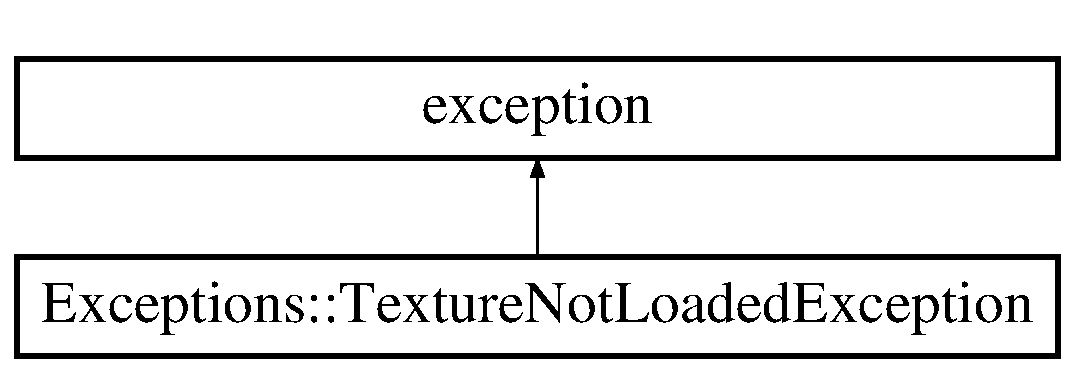
\includegraphics[height=2.000000cm]{class_exceptions_1_1_texture_not_loaded_exception}
\end{center}
\end{figure}
\subsection*{Public Member Functions}
\begin{DoxyCompactItemize}
\item 
\hyperlink{class_exceptions_1_1_texture_not_loaded_exception_a9375ca8c5b0a5cb294b7a8c295cf29b3}{Texture\+Not\+Loaded\+Exception} ()
\item 
virtual const char $\ast$ \hyperlink{class_exceptions_1_1_texture_not_loaded_exception_ae7b8bc33fa55d2b81ee8b9705bbaab97}{what} () const   throw ()
\end{DoxyCompactItemize}


\subsection{Constructor \& Destructor Documentation}
\hypertarget{class_exceptions_1_1_texture_not_loaded_exception_a9375ca8c5b0a5cb294b7a8c295cf29b3}{}\index{Exceptions\+::\+Texture\+Not\+Loaded\+Exception@{Exceptions\+::\+Texture\+Not\+Loaded\+Exception}!Texture\+Not\+Loaded\+Exception@{Texture\+Not\+Loaded\+Exception}}
\index{Texture\+Not\+Loaded\+Exception@{Texture\+Not\+Loaded\+Exception}!Exceptions\+::\+Texture\+Not\+Loaded\+Exception@{Exceptions\+::\+Texture\+Not\+Loaded\+Exception}}
\subsubsection[{Texture\+Not\+Loaded\+Exception}]{\setlength{\rightskip}{0pt plus 5cm}Exceptions\+::\+Texture\+Not\+Loaded\+Exception\+::\+Texture\+Not\+Loaded\+Exception (
\begin{DoxyParamCaption}
{}
\end{DoxyParamCaption}
)\hspace{0.3cm}{\ttfamily [inline]}}\label{class_exceptions_1_1_texture_not_loaded_exception_a9375ca8c5b0a5cb294b7a8c295cf29b3}


\subsection{Member Function Documentation}
\hypertarget{class_exceptions_1_1_texture_not_loaded_exception_ae7b8bc33fa55d2b81ee8b9705bbaab97}{}\index{Exceptions\+::\+Texture\+Not\+Loaded\+Exception@{Exceptions\+::\+Texture\+Not\+Loaded\+Exception}!what@{what}}
\index{what@{what}!Exceptions\+::\+Texture\+Not\+Loaded\+Exception@{Exceptions\+::\+Texture\+Not\+Loaded\+Exception}}
\subsubsection[{what}]{\setlength{\rightskip}{0pt plus 5cm}virtual const char$\ast$ Exceptions\+::\+Texture\+Not\+Loaded\+Exception\+::what (
\begin{DoxyParamCaption}
{}
\end{DoxyParamCaption}
) const throw  ) \hspace{0.3cm}{\ttfamily [inline]}, {\ttfamily [virtual]}}\label{class_exceptions_1_1_texture_not_loaded_exception_ae7b8bc33fa55d2b81ee8b9705bbaab97}


The documentation for this class was generated from the following file\+:\begin{DoxyCompactItemize}
\item 
src/exceptions/\hyperlink{texture__not__loaded__exception_8h}{texture\+\_\+not\+\_\+loaded\+\_\+exception.\+h}\end{DoxyCompactItemize}

\hypertarget{class_graphics_1_1_tile}{}\section{Graphics\+:\+:Tile Class Reference}
\label{class_graphics_1_1_tile}\index{Graphics\+::\+Tile@{Graphics\+::\+Tile}}


{\ttfamily \#include $<$tile.\+h$>$}

Inheritance diagram for Graphics\+:\+:Tile\+:\begin{figure}[H]
\begin{center}
\leavevmode
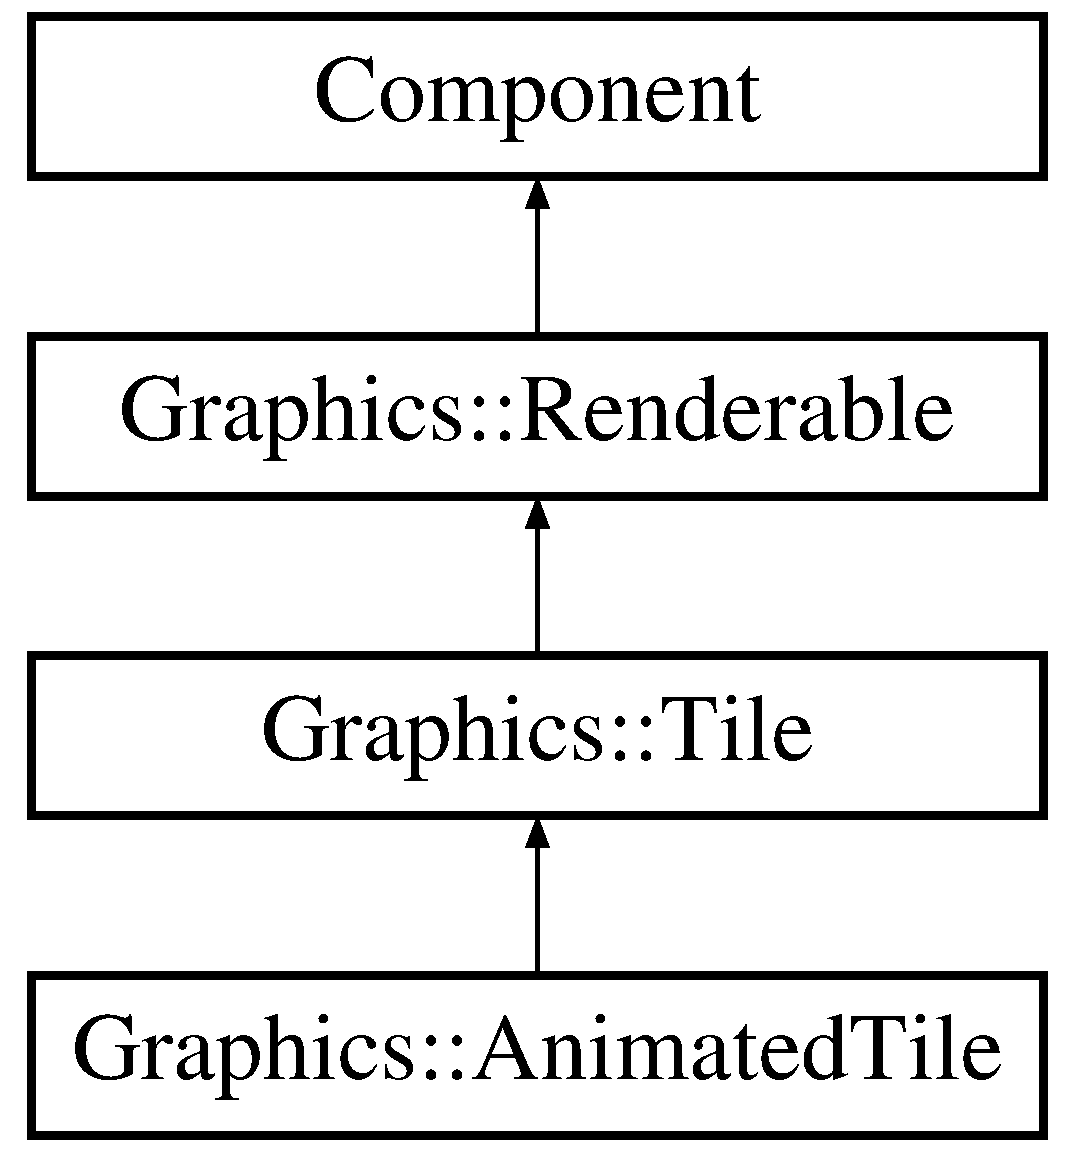
\includegraphics[height=4.000000cm]{class_graphics_1_1_tile}
\end{center}
\end{figure}
\subsection*{Public Member Functions}
\begin{DoxyCompactItemize}
\item 
\hyperlink{class_graphics_1_1_tile_a86a26aa6bec494b668d20be672843fee}{Tile} ()=delete
\item 
\hyperlink{class_graphics_1_1_tile_a861a8afb0c7322b145614c5c119a140a}{Tile} (const unsigned int \hyperlink{class_graphics_1_1_renderable_aabfa91ebff7b10decd54119d663044ef}{vertex\+\_\+array\+\_\+object}, const \hyperlink{class_graphics_1_1_vertex_data}{Vertex\+Data} \&data)
\item 
virtual \hyperlink{class_graphics_1_1_tile_a2bc2b71c90b1067ebc7f2f5fbf871524}{$\sim$\+Tile} ()
\item 
virtual void \hyperlink{class_graphics_1_1_tile_a28f5bdfa2fc61b292dda7ec15316b981}{on\+Destroy} () override
\item 
virtual const bool \hyperlink{class_graphics_1_1_tile_a0311b1d9548f6badc9e81820b110cbb4}{on\+Update} (const double delta) override
\begin{DoxyCompactList}\small\item\em \mbox{[}brief description\mbox{]} \end{DoxyCompactList}\item 
void \hyperlink{class_graphics_1_1_tile_acb61c259a174f0fda3adef70be96cb23}{set\+Size\+In\+Pixels} (const unsigned int size)
\item 
const unsigned int \hyperlink{class_graphics_1_1_tile_a0d490b7e8374d401b8fe8cbef57a6a3a}{size\+In\+Pixels} () const noexcept
\end{DoxyCompactItemize}
\subsection*{Private Attributes}
\begin{DoxyCompactItemize}
\item 
unsigned int \hyperlink{class_graphics_1_1_tile_a7524ad0a888622408b2447c70c4bbc86}{size\+\_\+pixels}
\end{DoxyCompactItemize}
\subsection*{Additional Inherited Members}


\subsection{Constructor \& Destructor Documentation}
\hypertarget{class_graphics_1_1_tile_a86a26aa6bec494b668d20be672843fee}{}\index{Graphics\+::\+Tile@{Graphics\+::\+Tile}!Tile@{Tile}}
\index{Tile@{Tile}!Graphics\+::\+Tile@{Graphics\+::\+Tile}}
\subsubsection[{Tile}]{\setlength{\rightskip}{0pt plus 5cm}Graphics\+::\+Tile\+::\+Tile (
\begin{DoxyParamCaption}
{}
\end{DoxyParamCaption}
)\hspace{0.3cm}{\ttfamily [delete]}}\label{class_graphics_1_1_tile_a86a26aa6bec494b668d20be672843fee}
\hypertarget{class_graphics_1_1_tile_a861a8afb0c7322b145614c5c119a140a}{}\index{Graphics\+::\+Tile@{Graphics\+::\+Tile}!Tile@{Tile}}
\index{Tile@{Tile}!Graphics\+::\+Tile@{Graphics\+::\+Tile}}
\subsubsection[{Tile}]{\setlength{\rightskip}{0pt plus 5cm}Graphics\+::\+Tile\+::\+Tile (
\begin{DoxyParamCaption}
\item[{const unsigned int}]{vertex\+\_\+array\+\_\+object, }
\item[{const {\bf Vertex\+Data} \&}]{data}
\end{DoxyParamCaption}
)}\label{class_graphics_1_1_tile_a861a8afb0c7322b145614c5c119a140a}
\hypertarget{class_graphics_1_1_tile_a2bc2b71c90b1067ebc7f2f5fbf871524}{}\index{Graphics\+::\+Tile@{Graphics\+::\+Tile}!````~Tile@{$\sim$\+Tile}}
\index{````~Tile@{$\sim$\+Tile}!Graphics\+::\+Tile@{Graphics\+::\+Tile}}
\subsubsection[{$\sim$\+Tile}]{\setlength{\rightskip}{0pt plus 5cm}Graphics\+::\+Tile\+::$\sim$\+Tile (
\begin{DoxyParamCaption}
{}
\end{DoxyParamCaption}
)\hspace{0.3cm}{\ttfamily [virtual]}}\label{class_graphics_1_1_tile_a2bc2b71c90b1067ebc7f2f5fbf871524}


\subsection{Member Function Documentation}
\hypertarget{class_graphics_1_1_tile_a28f5bdfa2fc61b292dda7ec15316b981}{}\index{Graphics\+::\+Tile@{Graphics\+::\+Tile}!on\+Destroy@{on\+Destroy}}
\index{on\+Destroy@{on\+Destroy}!Graphics\+::\+Tile@{Graphics\+::\+Tile}}
\subsubsection[{on\+Destroy}]{\setlength{\rightskip}{0pt plus 5cm}void Graphics\+::\+Tile\+::on\+Destroy (
\begin{DoxyParamCaption}
{}
\end{DoxyParamCaption}
)\hspace{0.3cm}{\ttfamily [override]}, {\ttfamily [virtual]}}\label{class_graphics_1_1_tile_a28f5bdfa2fc61b292dda7ec15316b981}


Reimplemented from \hyperlink{class_graphics_1_1_renderable_a6e20996de55215db7ffae2792aaaa88e}{Graphics\+::\+Renderable}.



Reimplemented in \hyperlink{class_graphics_1_1_animated_tile_a9781b9b256a666a123fd2c050adb5118}{Graphics\+::\+Animated\+Tile}.

\hypertarget{class_graphics_1_1_tile_a0311b1d9548f6badc9e81820b110cbb4}{}\index{Graphics\+::\+Tile@{Graphics\+::\+Tile}!on\+Update@{on\+Update}}
\index{on\+Update@{on\+Update}!Graphics\+::\+Tile@{Graphics\+::\+Tile}}
\subsubsection[{on\+Update}]{\setlength{\rightskip}{0pt plus 5cm}const bool Graphics\+::\+Tile\+::on\+Update (
\begin{DoxyParamCaption}
\item[{const double}]{delta}
\end{DoxyParamCaption}
)\hspace{0.3cm}{\ttfamily [override]}, {\ttfamily [virtual]}}\label{class_graphics_1_1_tile_a0311b1d9548f6badc9e81820b110cbb4}


\mbox{[}brief description\mbox{]} 

\mbox{[}long description\mbox{]} \begin{DoxyReturn}{Returns}
true if anything was updated, false if nothing was updated 
\end{DoxyReturn}


Reimplemented from \hyperlink{class_graphics_1_1_renderable_a7d0e820c55cb7f5c552aa0c1e846db76}{Graphics\+::\+Renderable}.



Reimplemented in \hyperlink{class_graphics_1_1_animated_tile_a2c6f7cd3866cad84b73ea5da8b92b76e}{Graphics\+::\+Animated\+Tile}.

\hypertarget{class_graphics_1_1_tile_acb61c259a174f0fda3adef70be96cb23}{}\index{Graphics\+::\+Tile@{Graphics\+::\+Tile}!set\+Size\+In\+Pixels@{set\+Size\+In\+Pixels}}
\index{set\+Size\+In\+Pixels@{set\+Size\+In\+Pixels}!Graphics\+::\+Tile@{Graphics\+::\+Tile}}
\subsubsection[{set\+Size\+In\+Pixels}]{\setlength{\rightskip}{0pt plus 5cm}void Graphics\+::\+Tile\+::set\+Size\+In\+Pixels (
\begin{DoxyParamCaption}
\item[{const unsigned int}]{size}
\end{DoxyParamCaption}
)}\label{class_graphics_1_1_tile_acb61c259a174f0fda3adef70be96cb23}
\hypertarget{class_graphics_1_1_tile_a0d490b7e8374d401b8fe8cbef57a6a3a}{}\index{Graphics\+::\+Tile@{Graphics\+::\+Tile}!size\+In\+Pixels@{size\+In\+Pixels}}
\index{size\+In\+Pixels@{size\+In\+Pixels}!Graphics\+::\+Tile@{Graphics\+::\+Tile}}
\subsubsection[{size\+In\+Pixels}]{\setlength{\rightskip}{0pt plus 5cm}const unsigned int Graphics\+::\+Tile\+::size\+In\+Pixels (
\begin{DoxyParamCaption}
{}
\end{DoxyParamCaption}
) const\hspace{0.3cm}{\ttfamily [noexcept]}}\label{class_graphics_1_1_tile_a0d490b7e8374d401b8fe8cbef57a6a3a}


\subsection{Member Data Documentation}
\hypertarget{class_graphics_1_1_tile_a7524ad0a888622408b2447c70c4bbc86}{}\index{Graphics\+::\+Tile@{Graphics\+::\+Tile}!size\+\_\+pixels@{size\+\_\+pixels}}
\index{size\+\_\+pixels@{size\+\_\+pixels}!Graphics\+::\+Tile@{Graphics\+::\+Tile}}
\subsubsection[{size\+\_\+pixels}]{\setlength{\rightskip}{0pt plus 5cm}unsigned int Graphics\+::\+Tile\+::size\+\_\+pixels\hspace{0.3cm}{\ttfamily [private]}}\label{class_graphics_1_1_tile_a7524ad0a888622408b2447c70c4bbc86}


The documentation for this class was generated from the following files\+:\begin{DoxyCompactItemize}
\item 
src/graphics/\hyperlink{tile_8h}{tile.\+h}\item 
src/graphics/\hyperlink{tile_8cpp}{tile.\+cpp}\end{DoxyCompactItemize}

\hypertarget{class_graphics_1_1_tile_attribute_trait}{}\section{Graphics\+:\+:Tile\+Attribute\+Trait Class Reference}
\label{class_graphics_1_1_tile_attribute_trait}\index{Graphics\+::\+Tile\+Attribute\+Trait@{Graphics\+::\+Tile\+Attribute\+Trait}}


{\ttfamily \#include $<$tile\+\_\+attribute\+\_\+trait.\+h$>$}

Inheritance diagram for Graphics\+:\+:Tile\+Attribute\+Trait\+:\begin{figure}[H]
\begin{center}
\leavevmode
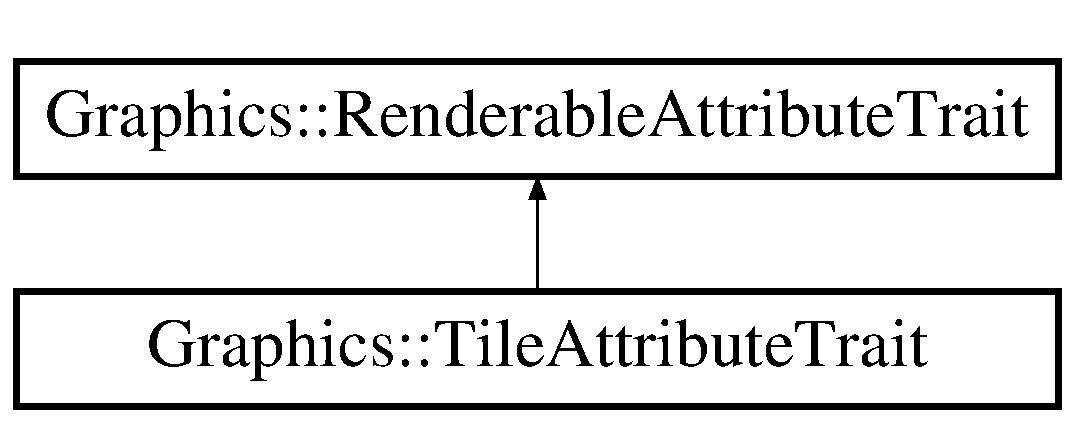
\includegraphics[height=2.000000cm]{class_graphics_1_1_tile_attribute_trait}
\end{center}
\end{figure}
\subsection*{Public Member Functions}
\begin{DoxyCompactItemize}
\item 
\hyperlink{class_graphics_1_1_tile_attribute_trait_a8271798aeb430ac5cf3dc1a0c73175fd}{Tile\+Attribute\+Trait} ()
\item 
virtual const std\+::map$<$ \hyperlink{class_graphics_1_1_vertex_data_a50e88236939dc2a3ec4df7aeb728620e}{Vertex\+Data\+::\+D\+A\+T\+A\+\_\+\+T\+Y\+P\+E}, unsigned int $>$ \hyperlink{class_graphics_1_1_tile_attribute_trait_a5c217a080f9b52799ad6c9e2ffaa06f5}{operator()} () const noexceptoverride
\end{DoxyCompactItemize}
\subsection*{Private Attributes}
\begin{DoxyCompactItemize}
\item 
std\+::map$<$ \hyperlink{class_graphics_1_1_vertex_data_a50e88236939dc2a3ec4df7aeb728620e}{Vertex\+Data\+::\+D\+A\+T\+A\+\_\+\+T\+Y\+P\+E}, unsigned int $>$ \hyperlink{class_graphics_1_1_tile_attribute_trait_a207820d288507ca70df8f95d7fdd04db}{trait}
\end{DoxyCompactItemize}


\subsection{Constructor \& Destructor Documentation}
\hypertarget{class_graphics_1_1_tile_attribute_trait_a8271798aeb430ac5cf3dc1a0c73175fd}{}\index{Graphics\+::\+Tile\+Attribute\+Trait@{Graphics\+::\+Tile\+Attribute\+Trait}!Tile\+Attribute\+Trait@{Tile\+Attribute\+Trait}}
\index{Tile\+Attribute\+Trait@{Tile\+Attribute\+Trait}!Graphics\+::\+Tile\+Attribute\+Trait@{Graphics\+::\+Tile\+Attribute\+Trait}}
\subsubsection[{Tile\+Attribute\+Trait}]{\setlength{\rightskip}{0pt plus 5cm}Graphics\+::\+Tile\+Attribute\+Trait\+::\+Tile\+Attribute\+Trait (
\begin{DoxyParamCaption}
{}
\end{DoxyParamCaption}
)\hspace{0.3cm}{\ttfamily [inline]}}\label{class_graphics_1_1_tile_attribute_trait_a8271798aeb430ac5cf3dc1a0c73175fd}


\subsection{Member Function Documentation}
\hypertarget{class_graphics_1_1_tile_attribute_trait_a5c217a080f9b52799ad6c9e2ffaa06f5}{}\index{Graphics\+::\+Tile\+Attribute\+Trait@{Graphics\+::\+Tile\+Attribute\+Trait}!operator()@{operator()}}
\index{operator()@{operator()}!Graphics\+::\+Tile\+Attribute\+Trait@{Graphics\+::\+Tile\+Attribute\+Trait}}
\subsubsection[{operator()}]{\setlength{\rightskip}{0pt plus 5cm}virtual const std\+::map$<${\bf Vertex\+Data\+::\+D\+A\+T\+A\+\_\+\+T\+Y\+P\+E}, unsigned int$>$ Graphics\+::\+Tile\+Attribute\+Trait\+::operator() (
\begin{DoxyParamCaption}
{}
\end{DoxyParamCaption}
) const\hspace{0.3cm}{\ttfamily [inline]}, {\ttfamily [override]}, {\ttfamily [virtual]}, {\ttfamily [noexcept]}}\label{class_graphics_1_1_tile_attribute_trait_a5c217a080f9b52799ad6c9e2ffaa06f5}


Implements \hyperlink{class_graphics_1_1_base_attribute_trait_a7f43cabd619b64be1a0056e0fe568cf5}{Graphics\+::\+Base\+Attribute\+Trait}.



\subsection{Member Data Documentation}
\hypertarget{class_graphics_1_1_tile_attribute_trait_a207820d288507ca70df8f95d7fdd04db}{}\index{Graphics\+::\+Tile\+Attribute\+Trait@{Graphics\+::\+Tile\+Attribute\+Trait}!trait@{trait}}
\index{trait@{trait}!Graphics\+::\+Tile\+Attribute\+Trait@{Graphics\+::\+Tile\+Attribute\+Trait}}
\subsubsection[{trait}]{\setlength{\rightskip}{0pt plus 5cm}std\+::map$<${\bf Vertex\+Data\+::\+D\+A\+T\+A\+\_\+\+T\+Y\+P\+E}, unsigned int$>$ Graphics\+::\+Tile\+Attribute\+Trait\+::trait\hspace{0.3cm}{\ttfamily [private]}}\label{class_graphics_1_1_tile_attribute_trait_a207820d288507ca70df8f95d7fdd04db}


The documentation for this class was generated from the following file\+:\begin{DoxyCompactItemize}
\item 
src/graphics/\hyperlink{tile__attribute__trait_8h}{tile\+\_\+attribute\+\_\+trait.\+h}\end{DoxyCompactItemize}

\hypertarget{class_transform}{}\section{Transform Class Reference}
\label{class_transform}\index{Transform@{Transform}}


{\ttfamily \#include $<$transform.\+h$>$}

Inheritance diagram for Transform\+:\begin{figure}[H]
\begin{center}
\leavevmode
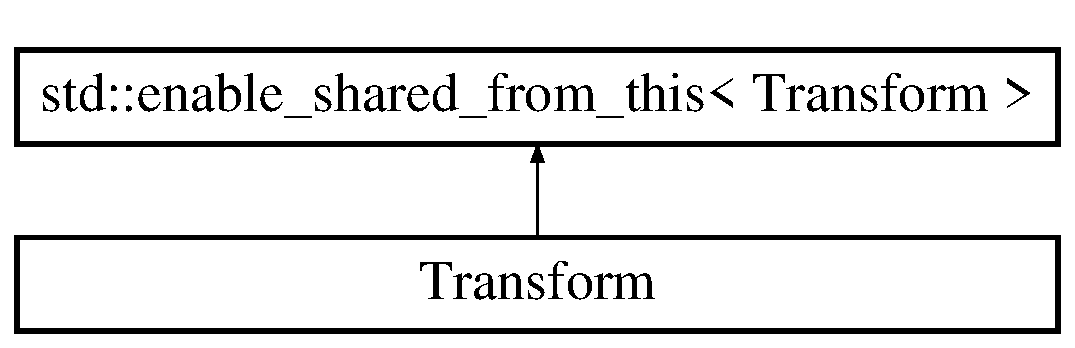
\includegraphics[height=2.000000cm]{class_transform}
\end{center}
\end{figure}
\subsection*{Public Member Functions}
\begin{DoxyCompactItemize}
\item 
\hyperlink{class_transform_aa08ca4266efabc768973cdeea51945ab}{Transform} ()
\item 
\hyperlink{class_transform_aa72e286c069850db80927b0e6554cd3e}{$\sim$\+Transform} ()
\item 
const bool \hyperlink{class_transform_a0ab0fe030d715fff815fb5cd2fad3951}{operator==} (const \hyperlink{class_transform}{Transform} \&other)
\item 
const bool \hyperlink{class_transform_aae84653176af974b257e44c832692501}{operator!=} (const \hyperlink{class_transform}{Transform} \&other)
\item 
void \hyperlink{class_transform_a56a4cdc7936c2654fc56c66a53f4432f}{add\+Child} (const std\+::shared\+\_\+ptr$<$ \hyperlink{class_transform}{Transform} $>$ \&transform)
\item 
void \hyperlink{class_transform_a9b4c664919e485ae51e244e8e9eb548d}{remove\+Child} (const std\+::shared\+\_\+ptr$<$ \hyperlink{class_transform}{Transform} $>$ \&transform)
\item 
std\+::list$<$ std\+::shared\+\_\+ptr$<$ \hyperlink{class_transform}{Transform} $>$ $>$ \hyperlink{class_transform_a8a4dd635e2fa7e652af05f13f22fe72b}{get\+Children} () const 
\item 
const unsigned int \hyperlink{class_transform_a4f9cf868bd8f7894ea28c4aae450cb69}{get\+Tree\+Size} () const 
\item 
{\footnotesize template$<$class T $>$ }\\void \hyperlink{class_transform_aafe00d06850ed594fcf0e44364f29224}{translate} (const T \&translation)
\item 
const glm\+::vec3 \hyperlink{class_transform_ad26386c52e4169a5f839a727c61e27a3}{get\+Absolute\+Translation} () const noexcept
\item 
const glm\+::vec3 \hyperlink{class_transform_a9abe479dcadead1d23c1335e8f042cea}{get\+Local\+Translation} () const noexcept
\item 
void \hyperlink{class_transform_a9b7f60043e6101b38888d9d760534626}{rotate} (const float angle, const glm\+::vec3 \&axis)
\item 
void \hyperlink{class_transform_a8f20b2aafd83175cb49eee9a14e55513}{rotate} (const float angle\+\_\+x, const float angle\+\_\+y, const float angle\+\_\+z)
\item 
void \hyperlink{class_transform_a2b4c1f2d0a62d0c89dedd88dbcdaa2d8}{rotate} (const glm\+::vec3 \&euler\+\_\+angles)
\item 
void \hyperlink{class_transform_ad51b8505353fa221c1a9d44590248e7e}{rotate} (const glm\+::quat \&quat)
\item 
const glm\+::quat \hyperlink{class_transform_adf0d22f16d1828804a038785d23aa782}{get\+Absolute\+Rotation} () const noexcept
\item 
const float \hyperlink{class_transform_abb2c3ea4aa73f73ee5a1e952e6ca572b}{get\+Absolute\+Rotation\+Angle} () const noexcept
\item 
const glm\+::vec3 \hyperlink{class_transform_aeeecb2d6949700678f7255a75e1aa109}{get\+Absolute\+Rotation\+Axis} () const noexcept
\item 
const glm\+::vec3 \hyperlink{class_transform_a680e2ca55154ee64067b637b3089a49a}{get\+Absolute\+Euler\+Angles} () const noexcept
\item 
const glm\+::quat \hyperlink{class_transform_af4c4efeddf0447ded7aedc65372691bc}{get\+Local\+Rotation} () const noexcept
\item 
const float \hyperlink{class_transform_adced558caa60dba283bc5711cd7f1357}{get\+Local\+Rotation\+Angle} () const noexcept
\item 
const glm\+::vec3 \hyperlink{class_transform_a861beae13233ea457e0eb906ac9f6ae5}{get\+Local\+Rotation\+Axis} () const noexcept
\item 
const glm\+::vec3 \hyperlink{class_transform_afd6613e7f6ecea657d9c4faf4b3772bd}{get\+Local\+Euler\+Angles} () const noexcept
\item 
{\footnotesize template$<$class T $>$ }\\void \hyperlink{class_transform_aa60a0073e2fd884226624f697ee31fe9}{scale} (const T \&scale)
\item 
const glm\+::vec3 \hyperlink{class_transform_a0c6436bf2df21cbf0675a86b84e3fb28}{get\+Absolute\+Scale} () const noexcept
\item 
const glm\+::vec3 \hyperlink{class_transform_aa9f7caf0eed7db1563ac72fc5726e2fe}{get\+Local\+Scale} () const noexcept
\item 
const glm\+::mat4 \hyperlink{class_transform_ab20c19ccdee7831086d2632a92eb078a}{get\+Absolute\+Transformation\+Matrix} () const noexcept
\item 
const glm\+::mat4 \hyperlink{class_transform_a503a33b8ca90f9e63d7f46c692561363}{get\+Local\+Transformation\+Matrix} () const noexcept
\item 
{\footnotesize template$<$$>$ }\\void \hyperlink{class_transform_aa32a94ec80690e270a849b0ae0fd9230}{translate} (const glm\+::vec2 \&translation)
\item 
{\footnotesize template$<$$>$ }\\void \hyperlink{class_transform_af72de2343b28c920935e085a369618f7}{translate} (const glm\+::vec3 \&translation)
\item 
{\footnotesize template$<$$>$ }\\void \hyperlink{class_transform_a80a0d4e1e53facf0576af6c7c0d7b3fe}{scale} (const glm\+::vec3 \&scale)
\item 
{\footnotesize template$<$$>$ }\\void \hyperlink{class_transform_ae246427e89c5a775fbb4981078410e29}{scale} (const glm\+::vec2 \&scale)
\item 
{\footnotesize template$<$$>$ }\\void \hyperlink{class_transform_a602ccc5ef9e53683bb7b9c6a4580f680}{scale} (const float \&scale)
\end{DoxyCompactItemize}
\subsection*{Private Attributes}
\begin{DoxyCompactItemize}
\item 
std\+::shared\+\_\+ptr$<$ \hyperlink{class_transform}{Transform} $>$ \hyperlink{class_transform_a71f8820c3ef3bd92f681bc92d200548f}{parent}
\item 
std\+::list$<$ std\+::shared\+\_\+ptr$<$ \hyperlink{class_transform}{Transform} $>$ $>$ \hyperlink{class_transform_a22f8ebd97bc4ab75e133d0490d88e240}{children}
\item 
glm\+::vec3 \hyperlink{class_transform_a9cab8178cfc03757f96fb805d3725a2f}{local\+\_\+translation}
\item 
glm\+::quat \hyperlink{class_transform_a363d6f26cde024731741bdfcafd77777}{local\+\_\+rotation}
\item 
glm\+::vec3 \hyperlink{class_transform_adc17f89af50a97d875020e34e2b1ca3d}{local\+\_\+scale}
\end{DoxyCompactItemize}


\subsection{Constructor \& Destructor Documentation}
\hypertarget{class_transform_aa08ca4266efabc768973cdeea51945ab}{}\index{Transform@{Transform}!Transform@{Transform}}
\index{Transform@{Transform}!Transform@{Transform}}
\subsubsection[{Transform}]{\setlength{\rightskip}{0pt plus 5cm}Transform\+::\+Transform (
\begin{DoxyParamCaption}
{}
\end{DoxyParamCaption}
)}\label{class_transform_aa08ca4266efabc768973cdeea51945ab}
\hypertarget{class_transform_aa72e286c069850db80927b0e6554cd3e}{}\index{Transform@{Transform}!````~Transform@{$\sim$\+Transform}}
\index{````~Transform@{$\sim$\+Transform}!Transform@{Transform}}
\subsubsection[{$\sim$\+Transform}]{\setlength{\rightskip}{0pt plus 5cm}Transform\+::$\sim$\+Transform (
\begin{DoxyParamCaption}
{}
\end{DoxyParamCaption}
)}\label{class_transform_aa72e286c069850db80927b0e6554cd3e}


\subsection{Member Function Documentation}
\hypertarget{class_transform_a56a4cdc7936c2654fc56c66a53f4432f}{}\index{Transform@{Transform}!add\+Child@{add\+Child}}
\index{add\+Child@{add\+Child}!Transform@{Transform}}
\subsubsection[{add\+Child}]{\setlength{\rightskip}{0pt plus 5cm}void Transform\+::add\+Child (
\begin{DoxyParamCaption}
\item[{const std\+::shared\+\_\+ptr$<$ {\bf Transform} $>$ \&}]{transform}
\end{DoxyParamCaption}
)}\label{class_transform_a56a4cdc7936c2654fc56c66a53f4432f}
\hypertarget{class_transform_a680e2ca55154ee64067b637b3089a49a}{}\index{Transform@{Transform}!get\+Absolute\+Euler\+Angles@{get\+Absolute\+Euler\+Angles}}
\index{get\+Absolute\+Euler\+Angles@{get\+Absolute\+Euler\+Angles}!Transform@{Transform}}
\subsubsection[{get\+Absolute\+Euler\+Angles}]{\setlength{\rightskip}{0pt plus 5cm}const glm\+::vec3 Transform\+::get\+Absolute\+Euler\+Angles (
\begin{DoxyParamCaption}
{}
\end{DoxyParamCaption}
) const\hspace{0.3cm}{\ttfamily [noexcept]}}\label{class_transform_a680e2ca55154ee64067b637b3089a49a}
\hypertarget{class_transform_adf0d22f16d1828804a038785d23aa782}{}\index{Transform@{Transform}!get\+Absolute\+Rotation@{get\+Absolute\+Rotation}}
\index{get\+Absolute\+Rotation@{get\+Absolute\+Rotation}!Transform@{Transform}}
\subsubsection[{get\+Absolute\+Rotation}]{\setlength{\rightskip}{0pt plus 5cm}const glm\+::quat Transform\+::get\+Absolute\+Rotation (
\begin{DoxyParamCaption}
{}
\end{DoxyParamCaption}
) const\hspace{0.3cm}{\ttfamily [noexcept]}}\label{class_transform_adf0d22f16d1828804a038785d23aa782}
\hypertarget{class_transform_abb2c3ea4aa73f73ee5a1e952e6ca572b}{}\index{Transform@{Transform}!get\+Absolute\+Rotation\+Angle@{get\+Absolute\+Rotation\+Angle}}
\index{get\+Absolute\+Rotation\+Angle@{get\+Absolute\+Rotation\+Angle}!Transform@{Transform}}
\subsubsection[{get\+Absolute\+Rotation\+Angle}]{\setlength{\rightskip}{0pt plus 5cm}const float Transform\+::get\+Absolute\+Rotation\+Angle (
\begin{DoxyParamCaption}
{}
\end{DoxyParamCaption}
) const\hspace{0.3cm}{\ttfamily [noexcept]}}\label{class_transform_abb2c3ea4aa73f73ee5a1e952e6ca572b}
\hypertarget{class_transform_aeeecb2d6949700678f7255a75e1aa109}{}\index{Transform@{Transform}!get\+Absolute\+Rotation\+Axis@{get\+Absolute\+Rotation\+Axis}}
\index{get\+Absolute\+Rotation\+Axis@{get\+Absolute\+Rotation\+Axis}!Transform@{Transform}}
\subsubsection[{get\+Absolute\+Rotation\+Axis}]{\setlength{\rightskip}{0pt plus 5cm}const glm\+::vec3 Transform\+::get\+Absolute\+Rotation\+Axis (
\begin{DoxyParamCaption}
{}
\end{DoxyParamCaption}
) const\hspace{0.3cm}{\ttfamily [noexcept]}}\label{class_transform_aeeecb2d6949700678f7255a75e1aa109}
\hypertarget{class_transform_a0c6436bf2df21cbf0675a86b84e3fb28}{}\index{Transform@{Transform}!get\+Absolute\+Scale@{get\+Absolute\+Scale}}
\index{get\+Absolute\+Scale@{get\+Absolute\+Scale}!Transform@{Transform}}
\subsubsection[{get\+Absolute\+Scale}]{\setlength{\rightskip}{0pt plus 5cm}const glm\+::vec3 Transform\+::get\+Absolute\+Scale (
\begin{DoxyParamCaption}
{}
\end{DoxyParamCaption}
) const\hspace{0.3cm}{\ttfamily [noexcept]}}\label{class_transform_a0c6436bf2df21cbf0675a86b84e3fb28}
\hypertarget{class_transform_ab20c19ccdee7831086d2632a92eb078a}{}\index{Transform@{Transform}!get\+Absolute\+Transformation\+Matrix@{get\+Absolute\+Transformation\+Matrix}}
\index{get\+Absolute\+Transformation\+Matrix@{get\+Absolute\+Transformation\+Matrix}!Transform@{Transform}}
\subsubsection[{get\+Absolute\+Transformation\+Matrix}]{\setlength{\rightskip}{0pt plus 5cm}const glm\+::mat4 Transform\+::get\+Absolute\+Transformation\+Matrix (
\begin{DoxyParamCaption}
{}
\end{DoxyParamCaption}
) const\hspace{0.3cm}{\ttfamily [noexcept]}}\label{class_transform_ab20c19ccdee7831086d2632a92eb078a}
\hypertarget{class_transform_ad26386c52e4169a5f839a727c61e27a3}{}\index{Transform@{Transform}!get\+Absolute\+Translation@{get\+Absolute\+Translation}}
\index{get\+Absolute\+Translation@{get\+Absolute\+Translation}!Transform@{Transform}}
\subsubsection[{get\+Absolute\+Translation}]{\setlength{\rightskip}{0pt plus 5cm}const glm\+::vec3 Transform\+::get\+Absolute\+Translation (
\begin{DoxyParamCaption}
{}
\end{DoxyParamCaption}
) const\hspace{0.3cm}{\ttfamily [noexcept]}}\label{class_transform_ad26386c52e4169a5f839a727c61e27a3}
\hypertarget{class_transform_a8a4dd635e2fa7e652af05f13f22fe72b}{}\index{Transform@{Transform}!get\+Children@{get\+Children}}
\index{get\+Children@{get\+Children}!Transform@{Transform}}
\subsubsection[{get\+Children}]{\setlength{\rightskip}{0pt plus 5cm}std\+::list$<$ std\+::shared\+\_\+ptr$<$ {\bf Transform} $>$ $>$ Transform\+::get\+Children (
\begin{DoxyParamCaption}
{}
\end{DoxyParamCaption}
) const}\label{class_transform_a8a4dd635e2fa7e652af05f13f22fe72b}
\hypertarget{class_transform_afd6613e7f6ecea657d9c4faf4b3772bd}{}\index{Transform@{Transform}!get\+Local\+Euler\+Angles@{get\+Local\+Euler\+Angles}}
\index{get\+Local\+Euler\+Angles@{get\+Local\+Euler\+Angles}!Transform@{Transform}}
\subsubsection[{get\+Local\+Euler\+Angles}]{\setlength{\rightskip}{0pt plus 5cm}const glm\+::vec3 Transform\+::get\+Local\+Euler\+Angles (
\begin{DoxyParamCaption}
{}
\end{DoxyParamCaption}
) const\hspace{0.3cm}{\ttfamily [noexcept]}}\label{class_transform_afd6613e7f6ecea657d9c4faf4b3772bd}
\hypertarget{class_transform_af4c4efeddf0447ded7aedc65372691bc}{}\index{Transform@{Transform}!get\+Local\+Rotation@{get\+Local\+Rotation}}
\index{get\+Local\+Rotation@{get\+Local\+Rotation}!Transform@{Transform}}
\subsubsection[{get\+Local\+Rotation}]{\setlength{\rightskip}{0pt plus 5cm}const glm\+::quat Transform\+::get\+Local\+Rotation (
\begin{DoxyParamCaption}
{}
\end{DoxyParamCaption}
) const\hspace{0.3cm}{\ttfamily [noexcept]}}\label{class_transform_af4c4efeddf0447ded7aedc65372691bc}
\hypertarget{class_transform_adced558caa60dba283bc5711cd7f1357}{}\index{Transform@{Transform}!get\+Local\+Rotation\+Angle@{get\+Local\+Rotation\+Angle}}
\index{get\+Local\+Rotation\+Angle@{get\+Local\+Rotation\+Angle}!Transform@{Transform}}
\subsubsection[{get\+Local\+Rotation\+Angle}]{\setlength{\rightskip}{0pt plus 5cm}const float Transform\+::get\+Local\+Rotation\+Angle (
\begin{DoxyParamCaption}
{}
\end{DoxyParamCaption}
) const\hspace{0.3cm}{\ttfamily [noexcept]}}\label{class_transform_adced558caa60dba283bc5711cd7f1357}
\hypertarget{class_transform_a861beae13233ea457e0eb906ac9f6ae5}{}\index{Transform@{Transform}!get\+Local\+Rotation\+Axis@{get\+Local\+Rotation\+Axis}}
\index{get\+Local\+Rotation\+Axis@{get\+Local\+Rotation\+Axis}!Transform@{Transform}}
\subsubsection[{get\+Local\+Rotation\+Axis}]{\setlength{\rightskip}{0pt plus 5cm}const glm\+::vec3 Transform\+::get\+Local\+Rotation\+Axis (
\begin{DoxyParamCaption}
{}
\end{DoxyParamCaption}
) const\hspace{0.3cm}{\ttfamily [noexcept]}}\label{class_transform_a861beae13233ea457e0eb906ac9f6ae5}
\hypertarget{class_transform_aa9f7caf0eed7db1563ac72fc5726e2fe}{}\index{Transform@{Transform}!get\+Local\+Scale@{get\+Local\+Scale}}
\index{get\+Local\+Scale@{get\+Local\+Scale}!Transform@{Transform}}
\subsubsection[{get\+Local\+Scale}]{\setlength{\rightskip}{0pt plus 5cm}const glm\+::vec3 Transform\+::get\+Local\+Scale (
\begin{DoxyParamCaption}
{}
\end{DoxyParamCaption}
) const\hspace{0.3cm}{\ttfamily [noexcept]}}\label{class_transform_aa9f7caf0eed7db1563ac72fc5726e2fe}
\hypertarget{class_transform_a503a33b8ca90f9e63d7f46c692561363}{}\index{Transform@{Transform}!get\+Local\+Transformation\+Matrix@{get\+Local\+Transformation\+Matrix}}
\index{get\+Local\+Transformation\+Matrix@{get\+Local\+Transformation\+Matrix}!Transform@{Transform}}
\subsubsection[{get\+Local\+Transformation\+Matrix}]{\setlength{\rightskip}{0pt plus 5cm}const glm\+::mat4 Transform\+::get\+Local\+Transformation\+Matrix (
\begin{DoxyParamCaption}
{}
\end{DoxyParamCaption}
) const\hspace{0.3cm}{\ttfamily [noexcept]}}\label{class_transform_a503a33b8ca90f9e63d7f46c692561363}
\hypertarget{class_transform_a9abe479dcadead1d23c1335e8f042cea}{}\index{Transform@{Transform}!get\+Local\+Translation@{get\+Local\+Translation}}
\index{get\+Local\+Translation@{get\+Local\+Translation}!Transform@{Transform}}
\subsubsection[{get\+Local\+Translation}]{\setlength{\rightskip}{0pt plus 5cm}const glm\+::vec3 Transform\+::get\+Local\+Translation (
\begin{DoxyParamCaption}
{}
\end{DoxyParamCaption}
) const\hspace{0.3cm}{\ttfamily [noexcept]}}\label{class_transform_a9abe479dcadead1d23c1335e8f042cea}
\hypertarget{class_transform_a4f9cf868bd8f7894ea28c4aae450cb69}{}\index{Transform@{Transform}!get\+Tree\+Size@{get\+Tree\+Size}}
\index{get\+Tree\+Size@{get\+Tree\+Size}!Transform@{Transform}}
\subsubsection[{get\+Tree\+Size}]{\setlength{\rightskip}{0pt plus 5cm}const unsigned int Transform\+::get\+Tree\+Size (
\begin{DoxyParamCaption}
{}
\end{DoxyParamCaption}
) const}\label{class_transform_a4f9cf868bd8f7894ea28c4aae450cb69}
\hypertarget{class_transform_aae84653176af974b257e44c832692501}{}\index{Transform@{Transform}!operator"!=@{operator"!=}}
\index{operator"!=@{operator"!=}!Transform@{Transform}}
\subsubsection[{operator"!=}]{\setlength{\rightskip}{0pt plus 5cm}const bool Transform\+::operator!= (
\begin{DoxyParamCaption}
\item[{const {\bf Transform} \&}]{other}
\end{DoxyParamCaption}
)}\label{class_transform_aae84653176af974b257e44c832692501}
\hypertarget{class_transform_a0ab0fe030d715fff815fb5cd2fad3951}{}\index{Transform@{Transform}!operator==@{operator==}}
\index{operator==@{operator==}!Transform@{Transform}}
\subsubsection[{operator==}]{\setlength{\rightskip}{0pt plus 5cm}const bool Transform\+::operator== (
\begin{DoxyParamCaption}
\item[{const {\bf Transform} \&}]{other}
\end{DoxyParamCaption}
)}\label{class_transform_a0ab0fe030d715fff815fb5cd2fad3951}
\hypertarget{class_transform_a9b4c664919e485ae51e244e8e9eb548d}{}\index{Transform@{Transform}!remove\+Child@{remove\+Child}}
\index{remove\+Child@{remove\+Child}!Transform@{Transform}}
\subsubsection[{remove\+Child}]{\setlength{\rightskip}{0pt plus 5cm}void Transform\+::remove\+Child (
\begin{DoxyParamCaption}
\item[{const std\+::shared\+\_\+ptr$<$ {\bf Transform} $>$ \&}]{transform}
\end{DoxyParamCaption}
)}\label{class_transform_a9b4c664919e485ae51e244e8e9eb548d}
\hypertarget{class_transform_a9b7f60043e6101b38888d9d760534626}{}\index{Transform@{Transform}!rotate@{rotate}}
\index{rotate@{rotate}!Transform@{Transform}}
\subsubsection[{rotate}]{\setlength{\rightskip}{0pt plus 5cm}void Transform\+::rotate (
\begin{DoxyParamCaption}
\item[{const float}]{angle, }
\item[{const glm\+::vec3 \&}]{axis}
\end{DoxyParamCaption}
)}\label{class_transform_a9b7f60043e6101b38888d9d760534626}
\hypertarget{class_transform_a8f20b2aafd83175cb49eee9a14e55513}{}\index{Transform@{Transform}!rotate@{rotate}}
\index{rotate@{rotate}!Transform@{Transform}}
\subsubsection[{rotate}]{\setlength{\rightskip}{0pt plus 5cm}void Transform\+::rotate (
\begin{DoxyParamCaption}
\item[{const float}]{angle\+\_\+x, }
\item[{const float}]{angle\+\_\+y, }
\item[{const float}]{angle\+\_\+z}
\end{DoxyParamCaption}
)}\label{class_transform_a8f20b2aafd83175cb49eee9a14e55513}
\hypertarget{class_transform_a2b4c1f2d0a62d0c89dedd88dbcdaa2d8}{}\index{Transform@{Transform}!rotate@{rotate}}
\index{rotate@{rotate}!Transform@{Transform}}
\subsubsection[{rotate}]{\setlength{\rightskip}{0pt plus 5cm}void Transform\+::rotate (
\begin{DoxyParamCaption}
\item[{const glm\+::vec3 \&}]{euler\+\_\+angles}
\end{DoxyParamCaption}
)}\label{class_transform_a2b4c1f2d0a62d0c89dedd88dbcdaa2d8}
\hypertarget{class_transform_ad51b8505353fa221c1a9d44590248e7e}{}\index{Transform@{Transform}!rotate@{rotate}}
\index{rotate@{rotate}!Transform@{Transform}}
\subsubsection[{rotate}]{\setlength{\rightskip}{0pt plus 5cm}void Transform\+::rotate (
\begin{DoxyParamCaption}
\item[{const glm\+::quat \&}]{quat}
\end{DoxyParamCaption}
)}\label{class_transform_ad51b8505353fa221c1a9d44590248e7e}
\hypertarget{class_transform_aa60a0073e2fd884226624f697ee31fe9}{}\index{Transform@{Transform}!scale@{scale}}
\index{scale@{scale}!Transform@{Transform}}
\subsubsection[{scale}]{\setlength{\rightskip}{0pt plus 5cm}template$<$class T $>$ void Transform\+::scale (
\begin{DoxyParamCaption}
\item[{const T \&}]{scale}
\end{DoxyParamCaption}
)}\label{class_transform_aa60a0073e2fd884226624f697ee31fe9}
\hypertarget{class_transform_a80a0d4e1e53facf0576af6c7c0d7b3fe}{}\index{Transform@{Transform}!scale@{scale}}
\index{scale@{scale}!Transform@{Transform}}
\subsubsection[{scale}]{\setlength{\rightskip}{0pt plus 5cm}template$<$$>$ void Transform\+::scale (
\begin{DoxyParamCaption}
\item[{const glm\+::vec3 \&}]{scale}
\end{DoxyParamCaption}
)}\label{class_transform_a80a0d4e1e53facf0576af6c7c0d7b3fe}
\hypertarget{class_transform_ae246427e89c5a775fbb4981078410e29}{}\index{Transform@{Transform}!scale@{scale}}
\index{scale@{scale}!Transform@{Transform}}
\subsubsection[{scale}]{\setlength{\rightskip}{0pt plus 5cm}template$<$$>$ void Transform\+::scale (
\begin{DoxyParamCaption}
\item[{const glm\+::vec2 \&}]{scale}
\end{DoxyParamCaption}
)}\label{class_transform_ae246427e89c5a775fbb4981078410e29}
\hypertarget{class_transform_a602ccc5ef9e53683bb7b9c6a4580f680}{}\index{Transform@{Transform}!scale@{scale}}
\index{scale@{scale}!Transform@{Transform}}
\subsubsection[{scale}]{\setlength{\rightskip}{0pt plus 5cm}template$<$$>$ void Transform\+::scale (
\begin{DoxyParamCaption}
\item[{const float \&}]{scale}
\end{DoxyParamCaption}
)}\label{class_transform_a602ccc5ef9e53683bb7b9c6a4580f680}
\hypertarget{class_transform_aafe00d06850ed594fcf0e44364f29224}{}\index{Transform@{Transform}!translate@{translate}}
\index{translate@{translate}!Transform@{Transform}}
\subsubsection[{translate}]{\setlength{\rightskip}{0pt plus 5cm}template$<$class T $>$ void Transform\+::translate (
\begin{DoxyParamCaption}
\item[{const T \&}]{translation}
\end{DoxyParamCaption}
)}\label{class_transform_aafe00d06850ed594fcf0e44364f29224}
\hypertarget{class_transform_aa32a94ec80690e270a849b0ae0fd9230}{}\index{Transform@{Transform}!translate@{translate}}
\index{translate@{translate}!Transform@{Transform}}
\subsubsection[{translate}]{\setlength{\rightskip}{0pt plus 5cm}template$<$$>$ void Transform\+::translate (
\begin{DoxyParamCaption}
\item[{const glm\+::vec2 \&}]{translation}
\end{DoxyParamCaption}
)}\label{class_transform_aa32a94ec80690e270a849b0ae0fd9230}
\hypertarget{class_transform_af72de2343b28c920935e085a369618f7}{}\index{Transform@{Transform}!translate@{translate}}
\index{translate@{translate}!Transform@{Transform}}
\subsubsection[{translate}]{\setlength{\rightskip}{0pt plus 5cm}template$<$$>$ void Transform\+::translate (
\begin{DoxyParamCaption}
\item[{const glm\+::vec3 \&}]{translation}
\end{DoxyParamCaption}
)}\label{class_transform_af72de2343b28c920935e085a369618f7}


\subsection{Member Data Documentation}
\hypertarget{class_transform_a22f8ebd97bc4ab75e133d0490d88e240}{}\index{Transform@{Transform}!children@{children}}
\index{children@{children}!Transform@{Transform}}
\subsubsection[{children}]{\setlength{\rightskip}{0pt plus 5cm}std\+::list$<$std\+::shared\+\_\+ptr$<${\bf Transform}$>$ $>$ Transform\+::children\hspace{0.3cm}{\ttfamily [private]}}\label{class_transform_a22f8ebd97bc4ab75e133d0490d88e240}
\hypertarget{class_transform_a363d6f26cde024731741bdfcafd77777}{}\index{Transform@{Transform}!local\+\_\+rotation@{local\+\_\+rotation}}
\index{local\+\_\+rotation@{local\+\_\+rotation}!Transform@{Transform}}
\subsubsection[{local\+\_\+rotation}]{\setlength{\rightskip}{0pt plus 5cm}glm\+::quat Transform\+::local\+\_\+rotation\hspace{0.3cm}{\ttfamily [private]}}\label{class_transform_a363d6f26cde024731741bdfcafd77777}
\hypertarget{class_transform_adc17f89af50a97d875020e34e2b1ca3d}{}\index{Transform@{Transform}!local\+\_\+scale@{local\+\_\+scale}}
\index{local\+\_\+scale@{local\+\_\+scale}!Transform@{Transform}}
\subsubsection[{local\+\_\+scale}]{\setlength{\rightskip}{0pt plus 5cm}glm\+::vec3 Transform\+::local\+\_\+scale\hspace{0.3cm}{\ttfamily [private]}}\label{class_transform_adc17f89af50a97d875020e34e2b1ca3d}
\hypertarget{class_transform_a9cab8178cfc03757f96fb805d3725a2f}{}\index{Transform@{Transform}!local\+\_\+translation@{local\+\_\+translation}}
\index{local\+\_\+translation@{local\+\_\+translation}!Transform@{Transform}}
\subsubsection[{local\+\_\+translation}]{\setlength{\rightskip}{0pt plus 5cm}glm\+::vec3 Transform\+::local\+\_\+translation\hspace{0.3cm}{\ttfamily [private]}}\label{class_transform_a9cab8178cfc03757f96fb805d3725a2f}
\hypertarget{class_transform_a71f8820c3ef3bd92f681bc92d200548f}{}\index{Transform@{Transform}!parent@{parent}}
\index{parent@{parent}!Transform@{Transform}}
\subsubsection[{parent}]{\setlength{\rightskip}{0pt plus 5cm}std\+::shared\+\_\+ptr$<${\bf Transform}$>$ Transform\+::parent\hspace{0.3cm}{\ttfamily [private]}}\label{class_transform_a71f8820c3ef3bd92f681bc92d200548f}


The documentation for this class was generated from the following files\+:\begin{DoxyCompactItemize}
\item 
src/\hyperlink{transform_8h}{transform.\+h}\item 
src/\hyperlink{transform_8cpp}{transform.\+cpp}\end{DoxyCompactItemize}

\hypertarget{class_graphics_1_1_triggerable_animations}{}\section{Graphics\+:\+:Triggerable\+Animations$<$ T $>$ Class Template Reference}
\label{class_graphics_1_1_triggerable_animations}\index{Graphics\+::\+Triggerable\+Animations$<$ T $>$@{Graphics\+::\+Triggerable\+Animations$<$ T $>$}}


{\ttfamily \#include $<$triggerable\+\_\+animations.\+hpp$>$}

\subsection*{Public Member Functions}
\begin{DoxyCompactItemize}
\item 
\hyperlink{class_graphics_1_1_triggerable_animations_a7efd5e939bef5de77f720f1e5b1114fe}{Triggerable\+Animations} ()=delete
\item 
\hyperlink{class_graphics_1_1_triggerable_animations_a8a2e951c4d6897ce273da003de9585ab}{Triggerable\+Animations} (const T \&start\+\_\+state)
\item 
void \hyperlink{class_graphics_1_1_triggerable_animations_a21d79b645121d0d316cae1112bddbce4}{initialize\+States} ()
\item 
void \hyperlink{class_graphics_1_1_triggerable_animations_ae34239042915beccc4c912f28a1d83e0}{trigger\+Tile} (const T \&state)
\end{DoxyCompactItemize}
\subsection*{Protected Member Functions}
\begin{DoxyCompactItemize}
\item 
void \hyperlink{class_graphics_1_1_triggerable_animations_ad7b21d0e24cfeb6279b91be187ddf2d1}{add\+Tile} (const T \&state, std\+::shared\+\_\+ptr$<$ \hyperlink{class_graphics_1_1_tile}{Graphics\+::\+Tile} $>$ tile)
\end{DoxyCompactItemize}
\subsection*{Protected Attributes}
\begin{DoxyCompactItemize}
\item 
T \hyperlink{class_graphics_1_1_triggerable_animations_a0f0e18726e1132c73d2e1d9f99072af1}{current\+\_\+state}
\end{DoxyCompactItemize}
\subsection*{Private Attributes}
\begin{DoxyCompactItemize}
\item 
std\+::map$<$ T, std\+::shared\+\_\+ptr$<$ \hyperlink{class_graphics_1_1_tile}{Graphics\+::\+Tile} $>$ $>$ \hyperlink{class_graphics_1_1_triggerable_animations_ad1d962d31d0515577f43b5b13b4b5743}{triggerable\+\_\+tiles}
\end{DoxyCompactItemize}


\subsection{Constructor \& Destructor Documentation}
\hypertarget{class_graphics_1_1_triggerable_animations_a7efd5e939bef5de77f720f1e5b1114fe}{}\index{Graphics\+::\+Triggerable\+Animations@{Graphics\+::\+Triggerable\+Animations}!Triggerable\+Animations@{Triggerable\+Animations}}
\index{Triggerable\+Animations@{Triggerable\+Animations}!Graphics\+::\+Triggerable\+Animations@{Graphics\+::\+Triggerable\+Animations}}
\subsubsection[{Triggerable\+Animations}]{\setlength{\rightskip}{0pt plus 5cm}template$<$typename T$>$ {\bf Graphics\+::\+Triggerable\+Animations}$<$ T $>$\+::{\bf Triggerable\+Animations} (
\begin{DoxyParamCaption}
{}
\end{DoxyParamCaption}
)\hspace{0.3cm}{\ttfamily [delete]}}\label{class_graphics_1_1_triggerable_animations_a7efd5e939bef5de77f720f1e5b1114fe}
\hypertarget{class_graphics_1_1_triggerable_animations_a8a2e951c4d6897ce273da003de9585ab}{}\index{Graphics\+::\+Triggerable\+Animations@{Graphics\+::\+Triggerable\+Animations}!Triggerable\+Animations@{Triggerable\+Animations}}
\index{Triggerable\+Animations@{Triggerable\+Animations}!Graphics\+::\+Triggerable\+Animations@{Graphics\+::\+Triggerable\+Animations}}
\subsubsection[{Triggerable\+Animations}]{\setlength{\rightskip}{0pt plus 5cm}template$<$typename T$>$ {\bf Graphics\+::\+Triggerable\+Animations}$<$ T $>$\+::{\bf Triggerable\+Animations} (
\begin{DoxyParamCaption}
\item[{const T \&}]{start\+\_\+state}
\end{DoxyParamCaption}
)\hspace{0.3cm}{\ttfamily [inline]}}\label{class_graphics_1_1_triggerable_animations_a8a2e951c4d6897ce273da003de9585ab}


\subsection{Member Function Documentation}
\hypertarget{class_graphics_1_1_triggerable_animations_ad7b21d0e24cfeb6279b91be187ddf2d1}{}\index{Graphics\+::\+Triggerable\+Animations@{Graphics\+::\+Triggerable\+Animations}!add\+Tile@{add\+Tile}}
\index{add\+Tile@{add\+Tile}!Graphics\+::\+Triggerable\+Animations@{Graphics\+::\+Triggerable\+Animations}}
\subsubsection[{add\+Tile}]{\setlength{\rightskip}{0pt plus 5cm}template$<$typename T$>$ void {\bf Graphics\+::\+Triggerable\+Animations}$<$ T $>$\+::add\+Tile (
\begin{DoxyParamCaption}
\item[{const T \&}]{state, }
\item[{std\+::shared\+\_\+ptr$<$ {\bf Graphics\+::\+Tile} $>$}]{tile}
\end{DoxyParamCaption}
)\hspace{0.3cm}{\ttfamily [inline]}, {\ttfamily [protected]}}\label{class_graphics_1_1_triggerable_animations_ad7b21d0e24cfeb6279b91be187ddf2d1}
\hypertarget{class_graphics_1_1_triggerable_animations_a21d79b645121d0d316cae1112bddbce4}{}\index{Graphics\+::\+Triggerable\+Animations@{Graphics\+::\+Triggerable\+Animations}!initialize\+States@{initialize\+States}}
\index{initialize\+States@{initialize\+States}!Graphics\+::\+Triggerable\+Animations@{Graphics\+::\+Triggerable\+Animations}}
\subsubsection[{initialize\+States}]{\setlength{\rightskip}{0pt plus 5cm}template$<$typename T$>$ void {\bf Graphics\+::\+Triggerable\+Animations}$<$ T $>$\+::initialize\+States (
\begin{DoxyParamCaption}
{}
\end{DoxyParamCaption}
)\hspace{0.3cm}{\ttfamily [inline]}}\label{class_graphics_1_1_triggerable_animations_a21d79b645121d0d316cae1112bddbce4}
\hypertarget{class_graphics_1_1_triggerable_animations_ae34239042915beccc4c912f28a1d83e0}{}\index{Graphics\+::\+Triggerable\+Animations@{Graphics\+::\+Triggerable\+Animations}!trigger\+Tile@{trigger\+Tile}}
\index{trigger\+Tile@{trigger\+Tile}!Graphics\+::\+Triggerable\+Animations@{Graphics\+::\+Triggerable\+Animations}}
\subsubsection[{trigger\+Tile}]{\setlength{\rightskip}{0pt plus 5cm}template$<$typename T$>$ void {\bf Graphics\+::\+Triggerable\+Animations}$<$ T $>$\+::trigger\+Tile (
\begin{DoxyParamCaption}
\item[{const T \&}]{state}
\end{DoxyParamCaption}
)\hspace{0.3cm}{\ttfamily [inline]}}\label{class_graphics_1_1_triggerable_animations_ae34239042915beccc4c912f28a1d83e0}


\subsection{Member Data Documentation}
\hypertarget{class_graphics_1_1_triggerable_animations_a0f0e18726e1132c73d2e1d9f99072af1}{}\index{Graphics\+::\+Triggerable\+Animations@{Graphics\+::\+Triggerable\+Animations}!current\+\_\+state@{current\+\_\+state}}
\index{current\+\_\+state@{current\+\_\+state}!Graphics\+::\+Triggerable\+Animations@{Graphics\+::\+Triggerable\+Animations}}
\subsubsection[{current\+\_\+state}]{\setlength{\rightskip}{0pt plus 5cm}template$<$typename T$>$ T {\bf Graphics\+::\+Triggerable\+Animations}$<$ T $>$\+::current\+\_\+state\hspace{0.3cm}{\ttfamily [protected]}}\label{class_graphics_1_1_triggerable_animations_a0f0e18726e1132c73d2e1d9f99072af1}
\hypertarget{class_graphics_1_1_triggerable_animations_ad1d962d31d0515577f43b5b13b4b5743}{}\index{Graphics\+::\+Triggerable\+Animations@{Graphics\+::\+Triggerable\+Animations}!triggerable\+\_\+tiles@{triggerable\+\_\+tiles}}
\index{triggerable\+\_\+tiles@{triggerable\+\_\+tiles}!Graphics\+::\+Triggerable\+Animations@{Graphics\+::\+Triggerable\+Animations}}
\subsubsection[{triggerable\+\_\+tiles}]{\setlength{\rightskip}{0pt plus 5cm}template$<$typename T$>$ std\+::map$<$T, std\+::shared\+\_\+ptr$<${\bf Graphics\+::\+Tile}$>$ $>$ {\bf Graphics\+::\+Triggerable\+Animations}$<$ T $>$\+::triggerable\+\_\+tiles\hspace{0.3cm}{\ttfamily [private]}}\label{class_graphics_1_1_triggerable_animations_ad1d962d31d0515577f43b5b13b4b5743}


The documentation for this class was generated from the following file\+:\begin{DoxyCompactItemize}
\item 
src/graphics/\hyperlink{triggerable__animations_8hpp}{triggerable\+\_\+animations.\+hpp}\end{DoxyCompactItemize}

\hypertarget{class_graphics_1_1_vertex_data}{}\section{Graphics\+:\+:Vertex\+Data Class Reference}
\label{class_graphics_1_1_vertex_data}\index{Graphics\+::\+Vertex\+Data@{Graphics\+::\+Vertex\+Data}}


{\ttfamily \#include $<$vertex\+\_\+data.\+h$>$}

\subsection*{Public Types}
\begin{DoxyCompactItemize}
\item 
enum \hyperlink{class_graphics_1_1_vertex_data_a50e88236939dc2a3ec4df7aeb728620e}{D\+A\+T\+A\+\_\+\+T\+Y\+P\+E} \+: unsigned char \{ \\*
\hyperlink{class_graphics_1_1_vertex_data_a50e88236939dc2a3ec4df7aeb728620eab4b2880ea86c8ee2eaceee4fbf35d3ac}{G\+E\+O\+M\+E\+T\+R\+Y} = 0, 
\hyperlink{class_graphics_1_1_vertex_data_a50e88236939dc2a3ec4df7aeb728620ea7b93224f58c43662f5be328f032d01e4}{T\+E\+X\+\_\+\+C\+O\+O\+R\+D\+S} = 1, 
\hyperlink{class_graphics_1_1_vertex_data_a50e88236939dc2a3ec4df7aeb728620ea0dbe0aa86a7dc55ca3aef237b0084068}{N\+O\+R\+M\+A\+L\+\_\+\+C\+O\+O\+R\+D\+S} = 2, 
\hyperlink{class_graphics_1_1_vertex_data_a50e88236939dc2a3ec4df7aeb728620ea77588319217115a8d9dead081e341e83}{R\+E\+S\+E\+R\+V\+E\+D1} = 3, 
\\*
\hyperlink{class_graphics_1_1_vertex_data_a50e88236939dc2a3ec4df7aeb728620ea9c6b6dd55ddf236f667e3e4019cda8d7}{R\+E\+S\+E\+R\+V\+E\+D2} = 4, 
\hyperlink{class_graphics_1_1_vertex_data_a50e88236939dc2a3ec4df7aeb728620eafc91ad501328ae49126c5d4bf850e537}{R\+E\+S\+E\+R\+V\+E\+D3} = 5, 
\hyperlink{class_graphics_1_1_vertex_data_a50e88236939dc2a3ec4df7aeb728620ea2185ed1920c6eeea484c4050e149764d}{R\+E\+S\+E\+R\+V\+E\+D4} = 6, 
\hyperlink{class_graphics_1_1_vertex_data_a50e88236939dc2a3ec4df7aeb728620ea92ff06fddd97b8c7d306ff7e912aeaba}{R\+E\+S\+E\+R\+V\+E\+D5} = 7, 
\\*
\hyperlink{class_graphics_1_1_vertex_data_a50e88236939dc2a3ec4df7aeb728620ea815ed3d3f65efe3a61a3df584a8fad55}{R\+E\+S\+E\+R\+V\+E\+D6} = 8, 
\hyperlink{class_graphics_1_1_vertex_data_a50e88236939dc2a3ec4df7aeb728620ead297e598e1a3dd7e9f7f3cc624130de9}{R\+E\+S\+E\+R\+V\+E\+D7} = 9, 
\hyperlink{class_graphics_1_1_vertex_data_a50e88236939dc2a3ec4df7aeb728620ea8f0a8e69a480d1dfb0f671acd6f72249}{R\+E\+S\+E\+R\+V\+E\+D8} = 10, 
\hyperlink{class_graphics_1_1_vertex_data_a50e88236939dc2a3ec4df7aeb728620eaeef1b1af84ab650ca26fcd90ed548642}{R\+E\+S\+E\+R\+V\+E\+D9} = 11, 
\\*
\hyperlink{class_graphics_1_1_vertex_data_a50e88236939dc2a3ec4df7aeb728620eaca1c371d86cb760f697bc8f9269ccc3a}{O\+N\+E\+\_\+\+W\+I\+D\+E} = 12, 
\hyperlink{class_graphics_1_1_vertex_data_a50e88236939dc2a3ec4df7aeb728620eaf411c36479247811d74f8c389cf22a9e}{T\+W\+O\+\_\+\+W\+I\+D\+E} = 13, 
\hyperlink{class_graphics_1_1_vertex_data_a50e88236939dc2a3ec4df7aeb728620eaed7cce23f542ae67236d1f0612bedce3}{T\+H\+R\+E\+E\+\_\+\+W\+I\+D\+E} = 14, 
\hyperlink{class_graphics_1_1_vertex_data_a50e88236939dc2a3ec4df7aeb728620eabcba96d8df23979f402ee0d3fbc22357}{F\+O\+U\+R\+\_\+\+W\+I\+D\+E} = 15
 \}
\end{DoxyCompactItemize}
\subsection*{Public Member Functions}
\begin{DoxyCompactItemize}
\item 
\hyperlink{class_graphics_1_1_vertex_data_a5f7a4162413a61c94cba76b528c17cc6}{Vertex\+Data} ()=delete
\item 
\hyperlink{class_graphics_1_1_vertex_data_aab133d7bc7567df43e6055f81e2ed23c}{Vertex\+Data} (const G\+Lenum \hyperlink{class_graphics_1_1_vertex_data_a3940832a3699c42ea2d9f4e0943653aa}{primitive\+\_\+type})
\item 
\hyperlink{class_graphics_1_1_vertex_data_aaf7331434454cb253f5ad5b86a8eec99}{Vertex\+Data} (const \hyperlink{class_graphics_1_1_vertex_data}{Vertex\+Data} \&vertex\+\_\+data)
\item 
\hyperlink{class_graphics_1_1_vertex_data}{Vertex\+Data} \hyperlink{class_graphics_1_1_vertex_data_abda73a49d1b280ee091afd53973c3448}{operator=} (const \hyperlink{class_graphics_1_1_vertex_data}{Vertex\+Data} \&vertex\+\_\+data)
\item 
\hyperlink{class_graphics_1_1_vertex_data_a59b5214fe3d6b6f9425032c86abf65cb}{$\sim$\+Vertex\+Data} ()
\item 
const bool \hyperlink{class_graphics_1_1_vertex_data_ad58ef98925908992fcd3ff090f57693f}{operator==} (const \hyperlink{class_graphics_1_1_vertex_data}{Vertex\+Data} \&other)
\item 
const bool \hyperlink{class_graphics_1_1_vertex_data_ac03511a02af7005757f60783b73fc51f}{operator!=} (const \hyperlink{class_graphics_1_1_vertex_data}{Vertex\+Data} \&other)
\item 
void \hyperlink{class_graphics_1_1_vertex_data_a9d7dfbf44faa4ebeeb052d9a49ec72c4}{add\+Indices} (const std\+::vector$<$ unsigned int $>$ \&\hyperlink{class_graphics_1_1_vertex_data_a9b777aa4bf035e805b2957fbcd158842}{indices})
\item 
{\footnotesize template$<$typename T $>$ }\\void \hyperlink{class_graphics_1_1_vertex_data_a1432af05a48b67a06c711910bb495c6e}{add\+Vec} (\hyperlink{class_graphics_1_1_vertex_data_a50e88236939dc2a3ec4df7aeb728620e}{D\+A\+T\+A\+\_\+\+T\+Y\+P\+E} data\+\_\+type, const std\+::vector$<$ T $>$ \&vec)
\item 
const unsigned int \hyperlink{class_graphics_1_1_vertex_data_a0c58a46431db14740109e6cadb322e4e}{get\+Index\+Count} () const noexcept
\item 
const unsigned int \hyperlink{class_graphics_1_1_vertex_data_afc9fb219a54d93cc0796424bd9d1a7db}{get\+Vertex\+Count} () const noexcept
\item 
{\footnotesize template$<$typename T $>$ }\\std\+::map$<$ \hyperlink{class_graphics_1_1_vertex_data_a50e88236939dc2a3ec4df7aeb728620e}{D\+A\+T\+A\+\_\+\+T\+Y\+P\+E}, std\+::vector$<$ T $>$ $>$ \hyperlink{class_graphics_1_1_vertex_data_a860575a29aa889f2a1028f2b8a255adc}{get\+Collapsed\+Vectors} () const 
\item 
std\+::vector$<$ unsigned int $>$ \hyperlink{class_graphics_1_1_vertex_data_a39b62d7b756b924aed1025d725a2316a}{get\+Indices} () const noexcept
\item 
unsigned int \hyperlink{class_graphics_1_1_vertex_data_ae46d393d65961b336a380d22bc8e39cb}{number\+Vertex\+Buffer\+Objects} () const noexcept
\item 
{\footnotesize template$<$$>$ }\\void \hyperlink{class_graphics_1_1_vertex_data_a3c16815abdf03faa1789af508f378b4a}{add\+Vec} (\hyperlink{class_graphics_1_1_vertex_data_a50e88236939dc2a3ec4df7aeb728620e}{Vertex\+Data\+::\+D\+A\+T\+A\+\_\+\+T\+Y\+P\+E} data\+\_\+type, const std\+::vector$<$ float $>$ \&vec)
\item 
{\footnotesize template$<$$>$ }\\void \hyperlink{class_graphics_1_1_vertex_data_a718710cb36c77da3ce7202fbf78f9dcf}{add\+Vec} (\hyperlink{class_graphics_1_1_vertex_data_a50e88236939dc2a3ec4df7aeb728620e}{Vertex\+Data\+::\+D\+A\+T\+A\+\_\+\+T\+Y\+P\+E} data\+\_\+type, const std\+::vector$<$ double $>$ \&vec)
\item 
{\footnotesize template$<$$>$ }\\void \hyperlink{class_graphics_1_1_vertex_data_addc04a692143dbd59ef3eb1b9107afc9}{add\+Vec} (\hyperlink{class_graphics_1_1_vertex_data_a50e88236939dc2a3ec4df7aeb728620e}{Vertex\+Data\+::\+D\+A\+T\+A\+\_\+\+T\+Y\+P\+E} data\+\_\+type, const std\+::vector$<$ int $>$ \&vec)
\item 
{\footnotesize template$<$$>$ }\\void \hyperlink{class_graphics_1_1_vertex_data_ad5b58302a2e592db88a896f8e8cbd83d}{add\+Vec} (\hyperlink{class_graphics_1_1_vertex_data_a50e88236939dc2a3ec4df7aeb728620e}{Vertex\+Data\+::\+D\+A\+T\+A\+\_\+\+T\+Y\+P\+E} data\+\_\+type, const std\+::vector$<$ unsigned int $>$ \&vec)
\item 
{\footnotesize template$<$$>$ }\\std\+::map$<$ \hyperlink{class_graphics_1_1_vertex_data_a50e88236939dc2a3ec4df7aeb728620e}{Vertex\+Data\+::\+D\+A\+T\+A\+\_\+\+T\+Y\+P\+E}, std\+::vector$<$ float $>$ $>$ \hyperlink{class_graphics_1_1_vertex_data_a248ab37b8eec5e4befba68c09a56fc1b}{get\+Collapsed\+Vectors} () const 
\item 
{\footnotesize template$<$$>$ }\\std\+::map$<$ \hyperlink{class_graphics_1_1_vertex_data_a50e88236939dc2a3ec4df7aeb728620e}{Vertex\+Data\+::\+D\+A\+T\+A\+\_\+\+T\+Y\+P\+E}, std\+::vector$<$ double $>$ $>$ \hyperlink{class_graphics_1_1_vertex_data_a460ef7490af53909849ede22d63f3144}{get\+Collapsed\+Vectors} () const 
\item 
{\footnotesize template$<$$>$ }\\std\+::map$<$ \hyperlink{class_graphics_1_1_vertex_data_a50e88236939dc2a3ec4df7aeb728620e}{Vertex\+Data\+::\+D\+A\+T\+A\+\_\+\+T\+Y\+P\+E}, std\+::vector$<$ int $>$ $>$ \hyperlink{class_graphics_1_1_vertex_data_a198830ed9c9eaadd45776b17bfa2909d}{get\+Collapsed\+Vectors} () const 
\item 
{\footnotesize template$<$$>$ }\\std\+::map$<$ \hyperlink{class_graphics_1_1_vertex_data_a50e88236939dc2a3ec4df7aeb728620e}{Vertex\+Data\+::\+D\+A\+T\+A\+\_\+\+T\+Y\+P\+E}, std\+::vector$<$ unsigned int $>$ $>$ \hyperlink{class_graphics_1_1_vertex_data_a1a056a887e89425563b93c7d14402a21}{get\+Collapsed\+Vectors} () const 
\end{DoxyCompactItemize}
\subsection*{Static Public Attributes}
\begin{DoxyCompactItemize}
\item 
static const std\+::map$<$ \hyperlink{class_graphics_1_1_vertex_data_a50e88236939dc2a3ec4df7aeb728620e}{D\+A\+T\+A\+\_\+\+T\+Y\+P\+E}, unsigned int $>$ \hyperlink{class_graphics_1_1_vertex_data_af49335b9e9bb94a48d1ade3e798278eb}{Data\+Width}
\end{DoxyCompactItemize}
\subsection*{Private Member Functions}
\begin{DoxyCompactItemize}
\item 
void \hyperlink{class_graphics_1_1_vertex_data_a90ba58b28b6981de0d841dfaff056bd9}{check\+Divisibility} (const unsigned int size)
\item 
void \hyperlink{class_graphics_1_1_vertex_data_a6bbb857b2a231cd75a236adfb553e976}{check\+Minimum} (const unsigned int size)
\item 
void \hyperlink{class_graphics_1_1_vertex_data_ac506af313dd521dfd05c566df3bf41bd}{clear\+Data\+Type} (const \hyperlink{class_graphics_1_1_vertex_data_a50e88236939dc2a3ec4df7aeb728620e}{D\+A\+T\+A\+\_\+\+T\+Y\+P\+E} \&type)
\item 
{\footnotesize template$<$class T $>$ }\\const bool \hyperlink{class_graphics_1_1_vertex_data_abe21332be8f7e42e9655c3271ddef0c0}{map\+Compare} (std\+::map$<$ \hyperlink{class_graphics_1_1_vertex_data_a50e88236939dc2a3ec4df7aeb728620e}{D\+A\+T\+A\+\_\+\+T\+Y\+P\+E}, std\+::vector$<$ T $>$$>$ lhs, std\+::map$<$ \hyperlink{class_graphics_1_1_vertex_data_a50e88236939dc2a3ec4df7aeb728620e}{D\+A\+T\+A\+\_\+\+T\+Y\+P\+E}, std\+::vector$<$ T $>$$>$ rhs)
\end{DoxyCompactItemize}
\subsection*{Private Attributes}
\begin{DoxyCompactItemize}
\item 
std\+::map$<$ \hyperlink{class_graphics_1_1_vertex_data_a50e88236939dc2a3ec4df7aeb728620e}{D\+A\+T\+A\+\_\+\+T\+Y\+P\+E}, std\+::vector$<$ float $>$ $>$ \hyperlink{class_graphics_1_1_vertex_data_a8dd7ba1a6fd4ba256b8805a2efa5f086}{float\+\_\+vector1s}
\item 
std\+::map$<$ \hyperlink{class_graphics_1_1_vertex_data_a50e88236939dc2a3ec4df7aeb728620e}{D\+A\+T\+A\+\_\+\+T\+Y\+P\+E}, std\+::vector$<$ glm\+::vec2 $>$ $>$ \hyperlink{class_graphics_1_1_vertex_data_add262a2473187fe32842cfc13e4eb72f}{float\+\_\+vector2s}
\item 
std\+::map$<$ \hyperlink{class_graphics_1_1_vertex_data_a50e88236939dc2a3ec4df7aeb728620e}{D\+A\+T\+A\+\_\+\+T\+Y\+P\+E}, std\+::vector$<$ glm\+::vec3 $>$ $>$ \hyperlink{class_graphics_1_1_vertex_data_a5d84c110b57a1c72bf871da376f8ef16}{float\+\_\+vector3s}
\item 
std\+::map$<$ \hyperlink{class_graphics_1_1_vertex_data_a50e88236939dc2a3ec4df7aeb728620e}{D\+A\+T\+A\+\_\+\+T\+Y\+P\+E}, std\+::vector$<$ glm\+::vec4 $>$ $>$ \hyperlink{class_graphics_1_1_vertex_data_a51c220f8d25f8f6f02a4024842579a7f}{float\+\_\+vector4s}
\item 
std\+::map$<$ \hyperlink{class_graphics_1_1_vertex_data_a50e88236939dc2a3ec4df7aeb728620e}{D\+A\+T\+A\+\_\+\+T\+Y\+P\+E}, std\+::vector$<$ double $>$ $>$ \hyperlink{class_graphics_1_1_vertex_data_ae9a48ea752fa50a024958139cc588c66}{double\+\_\+vector1s}
\item 
std\+::map$<$ \hyperlink{class_graphics_1_1_vertex_data_a50e88236939dc2a3ec4df7aeb728620e}{D\+A\+T\+A\+\_\+\+T\+Y\+P\+E}, std\+::vector$<$ glm\+::dvec2 $>$ $>$ \hyperlink{class_graphics_1_1_vertex_data_a0d9340ce408b8d5066524f440bc41067}{double\+\_\+vector2s}
\item 
std\+::map$<$ \hyperlink{class_graphics_1_1_vertex_data_a50e88236939dc2a3ec4df7aeb728620e}{D\+A\+T\+A\+\_\+\+T\+Y\+P\+E}, std\+::vector$<$ glm\+::dvec3 $>$ $>$ \hyperlink{class_graphics_1_1_vertex_data_acd623a5856ffac27e3cd51b4202def6d}{double\+\_\+vector3s}
\item 
std\+::map$<$ \hyperlink{class_graphics_1_1_vertex_data_a50e88236939dc2a3ec4df7aeb728620e}{D\+A\+T\+A\+\_\+\+T\+Y\+P\+E}, std\+::vector$<$ glm\+::dvec4 $>$ $>$ \hyperlink{class_graphics_1_1_vertex_data_a1b65aafda38402e62d0b52d7822492d9}{double\+\_\+vector4s}
\item 
std\+::map$<$ \hyperlink{class_graphics_1_1_vertex_data_a50e88236939dc2a3ec4df7aeb728620e}{D\+A\+T\+A\+\_\+\+T\+Y\+P\+E}, std\+::vector$<$ int $>$ $>$ \hyperlink{class_graphics_1_1_vertex_data_a9d162343dbfbfec79b69e2f0b5658b23}{int\+\_\+vector1s}
\item 
std\+::map$<$ \hyperlink{class_graphics_1_1_vertex_data_a50e88236939dc2a3ec4df7aeb728620e}{D\+A\+T\+A\+\_\+\+T\+Y\+P\+E}, std\+::vector$<$ glm\+::ivec2 $>$ $>$ \hyperlink{class_graphics_1_1_vertex_data_a2cefac20aaef5f2d926db3cf493ca607}{int\+\_\+vector2s}
\item 
std\+::map$<$ \hyperlink{class_graphics_1_1_vertex_data_a50e88236939dc2a3ec4df7aeb728620e}{D\+A\+T\+A\+\_\+\+T\+Y\+P\+E}, std\+::vector$<$ glm\+::ivec3 $>$ $>$ \hyperlink{class_graphics_1_1_vertex_data_a7bac97fce5e77e7850a5b4562a08ec0f}{int\+\_\+vector3s}
\item 
std\+::map$<$ \hyperlink{class_graphics_1_1_vertex_data_a50e88236939dc2a3ec4df7aeb728620e}{D\+A\+T\+A\+\_\+\+T\+Y\+P\+E}, std\+::vector$<$ glm\+::ivec4 $>$ $>$ \hyperlink{class_graphics_1_1_vertex_data_a40c1de9342a843c0e7a3d885d55f10f4}{int\+\_\+vector4s}
\item 
std\+::map$<$ \hyperlink{class_graphics_1_1_vertex_data_a50e88236939dc2a3ec4df7aeb728620e}{D\+A\+T\+A\+\_\+\+T\+Y\+P\+E}, std\+::vector$<$ unsigned int $>$ $>$ \hyperlink{class_graphics_1_1_vertex_data_abd5405c2b07bc0b93cf6fc05b2c5ce0c}{unsigned\+\_\+int\+\_\+vector1s}
\item 
std\+::map$<$ \hyperlink{class_graphics_1_1_vertex_data_a50e88236939dc2a3ec4df7aeb728620e}{D\+A\+T\+A\+\_\+\+T\+Y\+P\+E}, std\+::vector$<$ glm\+::uvec2 $>$ $>$ \hyperlink{class_graphics_1_1_vertex_data_a7c1edb826a504590a160d8a6d7ab9ae8}{unsigned\+\_\+int\+\_\+vector2s}
\item 
std\+::map$<$ \hyperlink{class_graphics_1_1_vertex_data_a50e88236939dc2a3ec4df7aeb728620e}{D\+A\+T\+A\+\_\+\+T\+Y\+P\+E}, std\+::vector$<$ glm\+::uvec3 $>$ $>$ \hyperlink{class_graphics_1_1_vertex_data_abe783ff7cc5377bef16e9962c64287a9}{unsigned\+\_\+int\+\_\+vector3s}
\item 
std\+::map$<$ \hyperlink{class_graphics_1_1_vertex_data_a50e88236939dc2a3ec4df7aeb728620e}{D\+A\+T\+A\+\_\+\+T\+Y\+P\+E}, std\+::vector$<$ glm\+::uvec4 $>$ $>$ \hyperlink{class_graphics_1_1_vertex_data_ac2a440c02a321387efa2d0028c151655}{unsigned\+\_\+int\+\_\+vector4s}
\item 
std\+::vector$<$ unsigned int $>$ \hyperlink{class_graphics_1_1_vertex_data_a9b777aa4bf035e805b2957fbcd158842}{indices}
\item 
unsigned int \hyperlink{class_graphics_1_1_vertex_data_ad998da458e1adca27ad17487e9ae38c6}{index\+\_\+count}
\item 
unsigned int \hyperlink{class_graphics_1_1_vertex_data_a82d5178d37db91235313309418f1ed8e}{vertex\+\_\+count}
\item 
G\+Lenum \hyperlink{class_graphics_1_1_vertex_data_a3940832a3699c42ea2d9f4e0943653aa}{primitive\+\_\+type}
\item 
const unsigned char \hyperlink{class_graphics_1_1_vertex_data_a0fc546e15f8fc02868e94246b93dd1b5}{A\+N\+Y} = 0
\item 
const std\+::map$<$ G\+Lenum, unsigned char $>$ \hyperlink{class_graphics_1_1_vertex_data_a4a88da3318b4c8deff9fa6168e75dd0a}{divisibility}
\item 
const std\+::map$<$ G\+Lenum, unsigned char $>$ \hyperlink{class_graphics_1_1_vertex_data_a65a814100217b32cc5a1f7a9bbd7f13c}{minimum}
\end{DoxyCompactItemize}


\subsection{Member Enumeration Documentation}
\hypertarget{class_graphics_1_1_vertex_data_a50e88236939dc2a3ec4df7aeb728620e}{}\index{Graphics\+::\+Vertex\+Data@{Graphics\+::\+Vertex\+Data}!D\+A\+T\+A\+\_\+\+T\+Y\+P\+E@{D\+A\+T\+A\+\_\+\+T\+Y\+P\+E}}
\index{D\+A\+T\+A\+\_\+\+T\+Y\+P\+E@{D\+A\+T\+A\+\_\+\+T\+Y\+P\+E}!Graphics\+::\+Vertex\+Data@{Graphics\+::\+Vertex\+Data}}
\subsubsection[{D\+A\+T\+A\+\_\+\+T\+Y\+P\+E}]{\setlength{\rightskip}{0pt plus 5cm}enum {\bf Graphics\+::\+Vertex\+Data\+::\+D\+A\+T\+A\+\_\+\+T\+Y\+P\+E} \+: unsigned char}\label{class_graphics_1_1_vertex_data_a50e88236939dc2a3ec4df7aeb728620e}
\begin{Desc}
\item[Enumerator]\par
\begin{description}
\index{G\+E\+O\+M\+E\+T\+R\+Y@{G\+E\+O\+M\+E\+T\+R\+Y}!Graphics\+::\+Vertex\+Data@{Graphics\+::\+Vertex\+Data}}\index{Graphics\+::\+Vertex\+Data@{Graphics\+::\+Vertex\+Data}!G\+E\+O\+M\+E\+T\+R\+Y@{G\+E\+O\+M\+E\+T\+R\+Y}}\item[{\em 
\hypertarget{class_graphics_1_1_vertex_data_a50e88236939dc2a3ec4df7aeb728620eab4b2880ea86c8ee2eaceee4fbf35d3ac}{}G\+E\+O\+M\+E\+T\+R\+Y\label{class_graphics_1_1_vertex_data_a50e88236939dc2a3ec4df7aeb728620eab4b2880ea86c8ee2eaceee4fbf35d3ac}
}]\index{T\+E\+X\+\_\+\+C\+O\+O\+R\+D\+S@{T\+E\+X\+\_\+\+C\+O\+O\+R\+D\+S}!Graphics\+::\+Vertex\+Data@{Graphics\+::\+Vertex\+Data}}\index{Graphics\+::\+Vertex\+Data@{Graphics\+::\+Vertex\+Data}!T\+E\+X\+\_\+\+C\+O\+O\+R\+D\+S@{T\+E\+X\+\_\+\+C\+O\+O\+R\+D\+S}}\item[{\em 
\hypertarget{class_graphics_1_1_vertex_data_a50e88236939dc2a3ec4df7aeb728620ea7b93224f58c43662f5be328f032d01e4}{}T\+E\+X\+\_\+\+C\+O\+O\+R\+D\+S\label{class_graphics_1_1_vertex_data_a50e88236939dc2a3ec4df7aeb728620ea7b93224f58c43662f5be328f032d01e4}
}]\index{N\+O\+R\+M\+A\+L\+\_\+\+C\+O\+O\+R\+D\+S@{N\+O\+R\+M\+A\+L\+\_\+\+C\+O\+O\+R\+D\+S}!Graphics\+::\+Vertex\+Data@{Graphics\+::\+Vertex\+Data}}\index{Graphics\+::\+Vertex\+Data@{Graphics\+::\+Vertex\+Data}!N\+O\+R\+M\+A\+L\+\_\+\+C\+O\+O\+R\+D\+S@{N\+O\+R\+M\+A\+L\+\_\+\+C\+O\+O\+R\+D\+S}}\item[{\em 
\hypertarget{class_graphics_1_1_vertex_data_a50e88236939dc2a3ec4df7aeb728620ea0dbe0aa86a7dc55ca3aef237b0084068}{}N\+O\+R\+M\+A\+L\+\_\+\+C\+O\+O\+R\+D\+S\label{class_graphics_1_1_vertex_data_a50e88236939dc2a3ec4df7aeb728620ea0dbe0aa86a7dc55ca3aef237b0084068}
}]\index{R\+E\+S\+E\+R\+V\+E\+D1@{R\+E\+S\+E\+R\+V\+E\+D1}!Graphics\+::\+Vertex\+Data@{Graphics\+::\+Vertex\+Data}}\index{Graphics\+::\+Vertex\+Data@{Graphics\+::\+Vertex\+Data}!R\+E\+S\+E\+R\+V\+E\+D1@{R\+E\+S\+E\+R\+V\+E\+D1}}\item[{\em 
\hypertarget{class_graphics_1_1_vertex_data_a50e88236939dc2a3ec4df7aeb728620ea77588319217115a8d9dead081e341e83}{}R\+E\+S\+E\+R\+V\+E\+D1\label{class_graphics_1_1_vertex_data_a50e88236939dc2a3ec4df7aeb728620ea77588319217115a8d9dead081e341e83}
}]\index{R\+E\+S\+E\+R\+V\+E\+D2@{R\+E\+S\+E\+R\+V\+E\+D2}!Graphics\+::\+Vertex\+Data@{Graphics\+::\+Vertex\+Data}}\index{Graphics\+::\+Vertex\+Data@{Graphics\+::\+Vertex\+Data}!R\+E\+S\+E\+R\+V\+E\+D2@{R\+E\+S\+E\+R\+V\+E\+D2}}\item[{\em 
\hypertarget{class_graphics_1_1_vertex_data_a50e88236939dc2a3ec4df7aeb728620ea9c6b6dd55ddf236f667e3e4019cda8d7}{}R\+E\+S\+E\+R\+V\+E\+D2\label{class_graphics_1_1_vertex_data_a50e88236939dc2a3ec4df7aeb728620ea9c6b6dd55ddf236f667e3e4019cda8d7}
}]\index{R\+E\+S\+E\+R\+V\+E\+D3@{R\+E\+S\+E\+R\+V\+E\+D3}!Graphics\+::\+Vertex\+Data@{Graphics\+::\+Vertex\+Data}}\index{Graphics\+::\+Vertex\+Data@{Graphics\+::\+Vertex\+Data}!R\+E\+S\+E\+R\+V\+E\+D3@{R\+E\+S\+E\+R\+V\+E\+D3}}\item[{\em 
\hypertarget{class_graphics_1_1_vertex_data_a50e88236939dc2a3ec4df7aeb728620eafc91ad501328ae49126c5d4bf850e537}{}R\+E\+S\+E\+R\+V\+E\+D3\label{class_graphics_1_1_vertex_data_a50e88236939dc2a3ec4df7aeb728620eafc91ad501328ae49126c5d4bf850e537}
}]\index{R\+E\+S\+E\+R\+V\+E\+D4@{R\+E\+S\+E\+R\+V\+E\+D4}!Graphics\+::\+Vertex\+Data@{Graphics\+::\+Vertex\+Data}}\index{Graphics\+::\+Vertex\+Data@{Graphics\+::\+Vertex\+Data}!R\+E\+S\+E\+R\+V\+E\+D4@{R\+E\+S\+E\+R\+V\+E\+D4}}\item[{\em 
\hypertarget{class_graphics_1_1_vertex_data_a50e88236939dc2a3ec4df7aeb728620ea2185ed1920c6eeea484c4050e149764d}{}R\+E\+S\+E\+R\+V\+E\+D4\label{class_graphics_1_1_vertex_data_a50e88236939dc2a3ec4df7aeb728620ea2185ed1920c6eeea484c4050e149764d}
}]\index{R\+E\+S\+E\+R\+V\+E\+D5@{R\+E\+S\+E\+R\+V\+E\+D5}!Graphics\+::\+Vertex\+Data@{Graphics\+::\+Vertex\+Data}}\index{Graphics\+::\+Vertex\+Data@{Graphics\+::\+Vertex\+Data}!R\+E\+S\+E\+R\+V\+E\+D5@{R\+E\+S\+E\+R\+V\+E\+D5}}\item[{\em 
\hypertarget{class_graphics_1_1_vertex_data_a50e88236939dc2a3ec4df7aeb728620ea92ff06fddd97b8c7d306ff7e912aeaba}{}R\+E\+S\+E\+R\+V\+E\+D5\label{class_graphics_1_1_vertex_data_a50e88236939dc2a3ec4df7aeb728620ea92ff06fddd97b8c7d306ff7e912aeaba}
}]\index{R\+E\+S\+E\+R\+V\+E\+D6@{R\+E\+S\+E\+R\+V\+E\+D6}!Graphics\+::\+Vertex\+Data@{Graphics\+::\+Vertex\+Data}}\index{Graphics\+::\+Vertex\+Data@{Graphics\+::\+Vertex\+Data}!R\+E\+S\+E\+R\+V\+E\+D6@{R\+E\+S\+E\+R\+V\+E\+D6}}\item[{\em 
\hypertarget{class_graphics_1_1_vertex_data_a50e88236939dc2a3ec4df7aeb728620ea815ed3d3f65efe3a61a3df584a8fad55}{}R\+E\+S\+E\+R\+V\+E\+D6\label{class_graphics_1_1_vertex_data_a50e88236939dc2a3ec4df7aeb728620ea815ed3d3f65efe3a61a3df584a8fad55}
}]\index{R\+E\+S\+E\+R\+V\+E\+D7@{R\+E\+S\+E\+R\+V\+E\+D7}!Graphics\+::\+Vertex\+Data@{Graphics\+::\+Vertex\+Data}}\index{Graphics\+::\+Vertex\+Data@{Graphics\+::\+Vertex\+Data}!R\+E\+S\+E\+R\+V\+E\+D7@{R\+E\+S\+E\+R\+V\+E\+D7}}\item[{\em 
\hypertarget{class_graphics_1_1_vertex_data_a50e88236939dc2a3ec4df7aeb728620ead297e598e1a3dd7e9f7f3cc624130de9}{}R\+E\+S\+E\+R\+V\+E\+D7\label{class_graphics_1_1_vertex_data_a50e88236939dc2a3ec4df7aeb728620ead297e598e1a3dd7e9f7f3cc624130de9}
}]\index{R\+E\+S\+E\+R\+V\+E\+D8@{R\+E\+S\+E\+R\+V\+E\+D8}!Graphics\+::\+Vertex\+Data@{Graphics\+::\+Vertex\+Data}}\index{Graphics\+::\+Vertex\+Data@{Graphics\+::\+Vertex\+Data}!R\+E\+S\+E\+R\+V\+E\+D8@{R\+E\+S\+E\+R\+V\+E\+D8}}\item[{\em 
\hypertarget{class_graphics_1_1_vertex_data_a50e88236939dc2a3ec4df7aeb728620ea8f0a8e69a480d1dfb0f671acd6f72249}{}R\+E\+S\+E\+R\+V\+E\+D8\label{class_graphics_1_1_vertex_data_a50e88236939dc2a3ec4df7aeb728620ea8f0a8e69a480d1dfb0f671acd6f72249}
}]\index{R\+E\+S\+E\+R\+V\+E\+D9@{R\+E\+S\+E\+R\+V\+E\+D9}!Graphics\+::\+Vertex\+Data@{Graphics\+::\+Vertex\+Data}}\index{Graphics\+::\+Vertex\+Data@{Graphics\+::\+Vertex\+Data}!R\+E\+S\+E\+R\+V\+E\+D9@{R\+E\+S\+E\+R\+V\+E\+D9}}\item[{\em 
\hypertarget{class_graphics_1_1_vertex_data_a50e88236939dc2a3ec4df7aeb728620eaeef1b1af84ab650ca26fcd90ed548642}{}R\+E\+S\+E\+R\+V\+E\+D9\label{class_graphics_1_1_vertex_data_a50e88236939dc2a3ec4df7aeb728620eaeef1b1af84ab650ca26fcd90ed548642}
}]\index{O\+N\+E\+\_\+\+W\+I\+D\+E@{O\+N\+E\+\_\+\+W\+I\+D\+E}!Graphics\+::\+Vertex\+Data@{Graphics\+::\+Vertex\+Data}}\index{Graphics\+::\+Vertex\+Data@{Graphics\+::\+Vertex\+Data}!O\+N\+E\+\_\+\+W\+I\+D\+E@{O\+N\+E\+\_\+\+W\+I\+D\+E}}\item[{\em 
\hypertarget{class_graphics_1_1_vertex_data_a50e88236939dc2a3ec4df7aeb728620eaca1c371d86cb760f697bc8f9269ccc3a}{}O\+N\+E\+\_\+\+W\+I\+D\+E\label{class_graphics_1_1_vertex_data_a50e88236939dc2a3ec4df7aeb728620eaca1c371d86cb760f697bc8f9269ccc3a}
}]\index{T\+W\+O\+\_\+\+W\+I\+D\+E@{T\+W\+O\+\_\+\+W\+I\+D\+E}!Graphics\+::\+Vertex\+Data@{Graphics\+::\+Vertex\+Data}}\index{Graphics\+::\+Vertex\+Data@{Graphics\+::\+Vertex\+Data}!T\+W\+O\+\_\+\+W\+I\+D\+E@{T\+W\+O\+\_\+\+W\+I\+D\+E}}\item[{\em 
\hypertarget{class_graphics_1_1_vertex_data_a50e88236939dc2a3ec4df7aeb728620eaf411c36479247811d74f8c389cf22a9e}{}T\+W\+O\+\_\+\+W\+I\+D\+E\label{class_graphics_1_1_vertex_data_a50e88236939dc2a3ec4df7aeb728620eaf411c36479247811d74f8c389cf22a9e}
}]\index{T\+H\+R\+E\+E\+\_\+\+W\+I\+D\+E@{T\+H\+R\+E\+E\+\_\+\+W\+I\+D\+E}!Graphics\+::\+Vertex\+Data@{Graphics\+::\+Vertex\+Data}}\index{Graphics\+::\+Vertex\+Data@{Graphics\+::\+Vertex\+Data}!T\+H\+R\+E\+E\+\_\+\+W\+I\+D\+E@{T\+H\+R\+E\+E\+\_\+\+W\+I\+D\+E}}\item[{\em 
\hypertarget{class_graphics_1_1_vertex_data_a50e88236939dc2a3ec4df7aeb728620eaed7cce23f542ae67236d1f0612bedce3}{}T\+H\+R\+E\+E\+\_\+\+W\+I\+D\+E\label{class_graphics_1_1_vertex_data_a50e88236939dc2a3ec4df7aeb728620eaed7cce23f542ae67236d1f0612bedce3}
}]\index{F\+O\+U\+R\+\_\+\+W\+I\+D\+E@{F\+O\+U\+R\+\_\+\+W\+I\+D\+E}!Graphics\+::\+Vertex\+Data@{Graphics\+::\+Vertex\+Data}}\index{Graphics\+::\+Vertex\+Data@{Graphics\+::\+Vertex\+Data}!F\+O\+U\+R\+\_\+\+W\+I\+D\+E@{F\+O\+U\+R\+\_\+\+W\+I\+D\+E}}\item[{\em 
\hypertarget{class_graphics_1_1_vertex_data_a50e88236939dc2a3ec4df7aeb728620eabcba96d8df23979f402ee0d3fbc22357}{}F\+O\+U\+R\+\_\+\+W\+I\+D\+E\label{class_graphics_1_1_vertex_data_a50e88236939dc2a3ec4df7aeb728620eabcba96d8df23979f402ee0d3fbc22357}
}]\end{description}
\end{Desc}


\subsection{Constructor \& Destructor Documentation}
\hypertarget{class_graphics_1_1_vertex_data_a5f7a4162413a61c94cba76b528c17cc6}{}\index{Graphics\+::\+Vertex\+Data@{Graphics\+::\+Vertex\+Data}!Vertex\+Data@{Vertex\+Data}}
\index{Vertex\+Data@{Vertex\+Data}!Graphics\+::\+Vertex\+Data@{Graphics\+::\+Vertex\+Data}}
\subsubsection[{Vertex\+Data}]{\setlength{\rightskip}{0pt plus 5cm}Graphics\+::\+Vertex\+Data\+::\+Vertex\+Data (
\begin{DoxyParamCaption}
{}
\end{DoxyParamCaption}
)\hspace{0.3cm}{\ttfamily [delete]}}\label{class_graphics_1_1_vertex_data_a5f7a4162413a61c94cba76b528c17cc6}
\hypertarget{class_graphics_1_1_vertex_data_aab133d7bc7567df43e6055f81e2ed23c}{}\index{Graphics\+::\+Vertex\+Data@{Graphics\+::\+Vertex\+Data}!Vertex\+Data@{Vertex\+Data}}
\index{Vertex\+Data@{Vertex\+Data}!Graphics\+::\+Vertex\+Data@{Graphics\+::\+Vertex\+Data}}
\subsubsection[{Vertex\+Data}]{\setlength{\rightskip}{0pt plus 5cm}Graphics\+::\+Vertex\+Data\+::\+Vertex\+Data (
\begin{DoxyParamCaption}
\item[{const G\+Lenum}]{primitive\+\_\+type}
\end{DoxyParamCaption}
)}\label{class_graphics_1_1_vertex_data_aab133d7bc7567df43e6055f81e2ed23c}
\hypertarget{class_graphics_1_1_vertex_data_aaf7331434454cb253f5ad5b86a8eec99}{}\index{Graphics\+::\+Vertex\+Data@{Graphics\+::\+Vertex\+Data}!Vertex\+Data@{Vertex\+Data}}
\index{Vertex\+Data@{Vertex\+Data}!Graphics\+::\+Vertex\+Data@{Graphics\+::\+Vertex\+Data}}
\subsubsection[{Vertex\+Data}]{\setlength{\rightskip}{0pt plus 5cm}Graphics\+::\+Vertex\+Data\+::\+Vertex\+Data (
\begin{DoxyParamCaption}
\item[{const {\bf Vertex\+Data} \&}]{vertex\+\_\+data}
\end{DoxyParamCaption}
)}\label{class_graphics_1_1_vertex_data_aaf7331434454cb253f5ad5b86a8eec99}
\hypertarget{class_graphics_1_1_vertex_data_a59b5214fe3d6b6f9425032c86abf65cb}{}\index{Graphics\+::\+Vertex\+Data@{Graphics\+::\+Vertex\+Data}!````~Vertex\+Data@{$\sim$\+Vertex\+Data}}
\index{````~Vertex\+Data@{$\sim$\+Vertex\+Data}!Graphics\+::\+Vertex\+Data@{Graphics\+::\+Vertex\+Data}}
\subsubsection[{$\sim$\+Vertex\+Data}]{\setlength{\rightskip}{0pt plus 5cm}Graphics\+::\+Vertex\+Data\+::$\sim$\+Vertex\+Data (
\begin{DoxyParamCaption}
{}
\end{DoxyParamCaption}
)}\label{class_graphics_1_1_vertex_data_a59b5214fe3d6b6f9425032c86abf65cb}


\subsection{Member Function Documentation}
\hypertarget{class_graphics_1_1_vertex_data_a9d7dfbf44faa4ebeeb052d9a49ec72c4}{}\index{Graphics\+::\+Vertex\+Data@{Graphics\+::\+Vertex\+Data}!add\+Indices@{add\+Indices}}
\index{add\+Indices@{add\+Indices}!Graphics\+::\+Vertex\+Data@{Graphics\+::\+Vertex\+Data}}
\subsubsection[{add\+Indices}]{\setlength{\rightskip}{0pt plus 5cm}void Graphics\+::\+Vertex\+Data\+::add\+Indices (
\begin{DoxyParamCaption}
\item[{const std\+::vector$<$ unsigned int $>$ \&}]{indices}
\end{DoxyParamCaption}
)}\label{class_graphics_1_1_vertex_data_a9d7dfbf44faa4ebeeb052d9a49ec72c4}
\hypertarget{class_graphics_1_1_vertex_data_a1432af05a48b67a06c711910bb495c6e}{}\index{Graphics\+::\+Vertex\+Data@{Graphics\+::\+Vertex\+Data}!add\+Vec@{add\+Vec}}
\index{add\+Vec@{add\+Vec}!Graphics\+::\+Vertex\+Data@{Graphics\+::\+Vertex\+Data}}
\subsubsection[{add\+Vec}]{\setlength{\rightskip}{0pt plus 5cm}template$<$typename T $>$ void Graphics\+::\+Vertex\+Data\+::add\+Vec (
\begin{DoxyParamCaption}
\item[{{\bf D\+A\+T\+A\+\_\+\+T\+Y\+P\+E}}]{data\+\_\+type, }
\item[{const std\+::vector$<$ T $>$ \&}]{vec}
\end{DoxyParamCaption}
)}\label{class_graphics_1_1_vertex_data_a1432af05a48b67a06c711910bb495c6e}
\hypertarget{class_graphics_1_1_vertex_data_a3c16815abdf03faa1789af508f378b4a}{}\index{Graphics\+::\+Vertex\+Data@{Graphics\+::\+Vertex\+Data}!add\+Vec@{add\+Vec}}
\index{add\+Vec@{add\+Vec}!Graphics\+::\+Vertex\+Data@{Graphics\+::\+Vertex\+Data}}
\subsubsection[{add\+Vec}]{\setlength{\rightskip}{0pt plus 5cm}template$<$$>$ void Graphics\+::\+Vertex\+Data\+::add\+Vec (
\begin{DoxyParamCaption}
\item[{{\bf Vertex\+Data\+::\+D\+A\+T\+A\+\_\+\+T\+Y\+P\+E}}]{data\+\_\+type, }
\item[{const std\+::vector$<$ float $>$ \&}]{vec}
\end{DoxyParamCaption}
)}\label{class_graphics_1_1_vertex_data_a3c16815abdf03faa1789af508f378b4a}
\hypertarget{class_graphics_1_1_vertex_data_a718710cb36c77da3ce7202fbf78f9dcf}{}\index{Graphics\+::\+Vertex\+Data@{Graphics\+::\+Vertex\+Data}!add\+Vec@{add\+Vec}}
\index{add\+Vec@{add\+Vec}!Graphics\+::\+Vertex\+Data@{Graphics\+::\+Vertex\+Data}}
\subsubsection[{add\+Vec}]{\setlength{\rightskip}{0pt plus 5cm}template$<$$>$ void Graphics\+::\+Vertex\+Data\+::add\+Vec (
\begin{DoxyParamCaption}
\item[{{\bf Vertex\+Data\+::\+D\+A\+T\+A\+\_\+\+T\+Y\+P\+E}}]{data\+\_\+type, }
\item[{const std\+::vector$<$ double $>$ \&}]{vec}
\end{DoxyParamCaption}
)}\label{class_graphics_1_1_vertex_data_a718710cb36c77da3ce7202fbf78f9dcf}
\hypertarget{class_graphics_1_1_vertex_data_addc04a692143dbd59ef3eb1b9107afc9}{}\index{Graphics\+::\+Vertex\+Data@{Graphics\+::\+Vertex\+Data}!add\+Vec@{add\+Vec}}
\index{add\+Vec@{add\+Vec}!Graphics\+::\+Vertex\+Data@{Graphics\+::\+Vertex\+Data}}
\subsubsection[{add\+Vec}]{\setlength{\rightskip}{0pt plus 5cm}template$<$$>$ void Graphics\+::\+Vertex\+Data\+::add\+Vec (
\begin{DoxyParamCaption}
\item[{{\bf Vertex\+Data\+::\+D\+A\+T\+A\+\_\+\+T\+Y\+P\+E}}]{data\+\_\+type, }
\item[{const std\+::vector$<$ int $>$ \&}]{vec}
\end{DoxyParamCaption}
)}\label{class_graphics_1_1_vertex_data_addc04a692143dbd59ef3eb1b9107afc9}
\hypertarget{class_graphics_1_1_vertex_data_ad5b58302a2e592db88a896f8e8cbd83d}{}\index{Graphics\+::\+Vertex\+Data@{Graphics\+::\+Vertex\+Data}!add\+Vec@{add\+Vec}}
\index{add\+Vec@{add\+Vec}!Graphics\+::\+Vertex\+Data@{Graphics\+::\+Vertex\+Data}}
\subsubsection[{add\+Vec}]{\setlength{\rightskip}{0pt plus 5cm}template$<$$>$ void Graphics\+::\+Vertex\+Data\+::add\+Vec (
\begin{DoxyParamCaption}
\item[{{\bf Vertex\+Data\+::\+D\+A\+T\+A\+\_\+\+T\+Y\+P\+E}}]{data\+\_\+type, }
\item[{const std\+::vector$<$ unsigned int $>$ \&}]{vec}
\end{DoxyParamCaption}
)}\label{class_graphics_1_1_vertex_data_ad5b58302a2e592db88a896f8e8cbd83d}
\hypertarget{class_graphics_1_1_vertex_data_a90ba58b28b6981de0d841dfaff056bd9}{}\index{Graphics\+::\+Vertex\+Data@{Graphics\+::\+Vertex\+Data}!check\+Divisibility@{check\+Divisibility}}
\index{check\+Divisibility@{check\+Divisibility}!Graphics\+::\+Vertex\+Data@{Graphics\+::\+Vertex\+Data}}
\subsubsection[{check\+Divisibility}]{\setlength{\rightskip}{0pt plus 5cm}void Graphics\+::\+Vertex\+Data\+::check\+Divisibility (
\begin{DoxyParamCaption}
\item[{const unsigned int}]{size}
\end{DoxyParamCaption}
)\hspace{0.3cm}{\ttfamily [private]}}\label{class_graphics_1_1_vertex_data_a90ba58b28b6981de0d841dfaff056bd9}
\hypertarget{class_graphics_1_1_vertex_data_a6bbb857b2a231cd75a236adfb553e976}{}\index{Graphics\+::\+Vertex\+Data@{Graphics\+::\+Vertex\+Data}!check\+Minimum@{check\+Minimum}}
\index{check\+Minimum@{check\+Minimum}!Graphics\+::\+Vertex\+Data@{Graphics\+::\+Vertex\+Data}}
\subsubsection[{check\+Minimum}]{\setlength{\rightskip}{0pt plus 5cm}void Graphics\+::\+Vertex\+Data\+::check\+Minimum (
\begin{DoxyParamCaption}
\item[{const unsigned int}]{size}
\end{DoxyParamCaption}
)\hspace{0.3cm}{\ttfamily [private]}}\label{class_graphics_1_1_vertex_data_a6bbb857b2a231cd75a236adfb553e976}
\hypertarget{class_graphics_1_1_vertex_data_ac506af313dd521dfd05c566df3bf41bd}{}\index{Graphics\+::\+Vertex\+Data@{Graphics\+::\+Vertex\+Data}!clear\+Data\+Type@{clear\+Data\+Type}}
\index{clear\+Data\+Type@{clear\+Data\+Type}!Graphics\+::\+Vertex\+Data@{Graphics\+::\+Vertex\+Data}}
\subsubsection[{clear\+Data\+Type}]{\setlength{\rightskip}{0pt plus 5cm}void Graphics\+::\+Vertex\+Data\+::clear\+Data\+Type (
\begin{DoxyParamCaption}
\item[{const {\bf D\+A\+T\+A\+\_\+\+T\+Y\+P\+E} \&}]{type}
\end{DoxyParamCaption}
)\hspace{0.3cm}{\ttfamily [private]}}\label{class_graphics_1_1_vertex_data_ac506af313dd521dfd05c566df3bf41bd}
\hypertarget{class_graphics_1_1_vertex_data_a860575a29aa889f2a1028f2b8a255adc}{}\index{Graphics\+::\+Vertex\+Data@{Graphics\+::\+Vertex\+Data}!get\+Collapsed\+Vectors@{get\+Collapsed\+Vectors}}
\index{get\+Collapsed\+Vectors@{get\+Collapsed\+Vectors}!Graphics\+::\+Vertex\+Data@{Graphics\+::\+Vertex\+Data}}
\subsubsection[{get\+Collapsed\+Vectors}]{\setlength{\rightskip}{0pt plus 5cm}template$<$typename T $>$ std\+::map$<${\bf D\+A\+T\+A\+\_\+\+T\+Y\+P\+E}, std\+::vector$<$T$>$ $>$ Graphics\+::\+Vertex\+Data\+::get\+Collapsed\+Vectors (
\begin{DoxyParamCaption}
{}
\end{DoxyParamCaption}
) const}\label{class_graphics_1_1_vertex_data_a860575a29aa889f2a1028f2b8a255adc}
\hypertarget{class_graphics_1_1_vertex_data_a248ab37b8eec5e4befba68c09a56fc1b}{}\index{Graphics\+::\+Vertex\+Data@{Graphics\+::\+Vertex\+Data}!get\+Collapsed\+Vectors@{get\+Collapsed\+Vectors}}
\index{get\+Collapsed\+Vectors@{get\+Collapsed\+Vectors}!Graphics\+::\+Vertex\+Data@{Graphics\+::\+Vertex\+Data}}
\subsubsection[{get\+Collapsed\+Vectors}]{\setlength{\rightskip}{0pt plus 5cm}template$<$$>$ std\+::map$<${\bf Vertex\+Data\+::\+D\+A\+T\+A\+\_\+\+T\+Y\+P\+E}, std\+::vector$<$float$>$ $>$ Graphics\+::\+Vertex\+Data\+::get\+Collapsed\+Vectors (
\begin{DoxyParamCaption}
{}
\end{DoxyParamCaption}
) const}\label{class_graphics_1_1_vertex_data_a248ab37b8eec5e4befba68c09a56fc1b}
\hypertarget{class_graphics_1_1_vertex_data_a460ef7490af53909849ede22d63f3144}{}\index{Graphics\+::\+Vertex\+Data@{Graphics\+::\+Vertex\+Data}!get\+Collapsed\+Vectors@{get\+Collapsed\+Vectors}}
\index{get\+Collapsed\+Vectors@{get\+Collapsed\+Vectors}!Graphics\+::\+Vertex\+Data@{Graphics\+::\+Vertex\+Data}}
\subsubsection[{get\+Collapsed\+Vectors}]{\setlength{\rightskip}{0pt plus 5cm}template$<$$>$ std\+::map$<${\bf Vertex\+Data\+::\+D\+A\+T\+A\+\_\+\+T\+Y\+P\+E}, std\+::vector$<$double$>$ $>$ Graphics\+::\+Vertex\+Data\+::get\+Collapsed\+Vectors (
\begin{DoxyParamCaption}
{}
\end{DoxyParamCaption}
) const}\label{class_graphics_1_1_vertex_data_a460ef7490af53909849ede22d63f3144}
\hypertarget{class_graphics_1_1_vertex_data_a198830ed9c9eaadd45776b17bfa2909d}{}\index{Graphics\+::\+Vertex\+Data@{Graphics\+::\+Vertex\+Data}!get\+Collapsed\+Vectors@{get\+Collapsed\+Vectors}}
\index{get\+Collapsed\+Vectors@{get\+Collapsed\+Vectors}!Graphics\+::\+Vertex\+Data@{Graphics\+::\+Vertex\+Data}}
\subsubsection[{get\+Collapsed\+Vectors}]{\setlength{\rightskip}{0pt plus 5cm}template$<$$>$ std\+::map$<${\bf Vertex\+Data\+::\+D\+A\+T\+A\+\_\+\+T\+Y\+P\+E}, std\+::vector$<$int$>$ $>$ Graphics\+::\+Vertex\+Data\+::get\+Collapsed\+Vectors (
\begin{DoxyParamCaption}
{}
\end{DoxyParamCaption}
) const}\label{class_graphics_1_1_vertex_data_a198830ed9c9eaadd45776b17bfa2909d}
\hypertarget{class_graphics_1_1_vertex_data_a1a056a887e89425563b93c7d14402a21}{}\index{Graphics\+::\+Vertex\+Data@{Graphics\+::\+Vertex\+Data}!get\+Collapsed\+Vectors@{get\+Collapsed\+Vectors}}
\index{get\+Collapsed\+Vectors@{get\+Collapsed\+Vectors}!Graphics\+::\+Vertex\+Data@{Graphics\+::\+Vertex\+Data}}
\subsubsection[{get\+Collapsed\+Vectors}]{\setlength{\rightskip}{0pt plus 5cm}template$<$$>$ std\+::map$<${\bf Vertex\+Data\+::\+D\+A\+T\+A\+\_\+\+T\+Y\+P\+E}, std\+::vector$<$unsigned int$>$ $>$ Graphics\+::\+Vertex\+Data\+::get\+Collapsed\+Vectors (
\begin{DoxyParamCaption}
{}
\end{DoxyParamCaption}
) const}\label{class_graphics_1_1_vertex_data_a1a056a887e89425563b93c7d14402a21}
\hypertarget{class_graphics_1_1_vertex_data_a0c58a46431db14740109e6cadb322e4e}{}\index{Graphics\+::\+Vertex\+Data@{Graphics\+::\+Vertex\+Data}!get\+Index\+Count@{get\+Index\+Count}}
\index{get\+Index\+Count@{get\+Index\+Count}!Graphics\+::\+Vertex\+Data@{Graphics\+::\+Vertex\+Data}}
\subsubsection[{get\+Index\+Count}]{\setlength{\rightskip}{0pt plus 5cm}const unsigned int Graphics\+::\+Vertex\+Data\+::get\+Index\+Count (
\begin{DoxyParamCaption}
{}
\end{DoxyParamCaption}
) const\hspace{0.3cm}{\ttfamily [noexcept]}}\label{class_graphics_1_1_vertex_data_a0c58a46431db14740109e6cadb322e4e}
\hypertarget{class_graphics_1_1_vertex_data_a39b62d7b756b924aed1025d725a2316a}{}\index{Graphics\+::\+Vertex\+Data@{Graphics\+::\+Vertex\+Data}!get\+Indices@{get\+Indices}}
\index{get\+Indices@{get\+Indices}!Graphics\+::\+Vertex\+Data@{Graphics\+::\+Vertex\+Data}}
\subsubsection[{get\+Indices}]{\setlength{\rightskip}{0pt plus 5cm}std\+::vector$<$ unsigned int $>$ Graphics\+::\+Vertex\+Data\+::get\+Indices (
\begin{DoxyParamCaption}
{}
\end{DoxyParamCaption}
) const\hspace{0.3cm}{\ttfamily [noexcept]}}\label{class_graphics_1_1_vertex_data_a39b62d7b756b924aed1025d725a2316a}
\hypertarget{class_graphics_1_1_vertex_data_afc9fb219a54d93cc0796424bd9d1a7db}{}\index{Graphics\+::\+Vertex\+Data@{Graphics\+::\+Vertex\+Data}!get\+Vertex\+Count@{get\+Vertex\+Count}}
\index{get\+Vertex\+Count@{get\+Vertex\+Count}!Graphics\+::\+Vertex\+Data@{Graphics\+::\+Vertex\+Data}}
\subsubsection[{get\+Vertex\+Count}]{\setlength{\rightskip}{0pt plus 5cm}const unsigned int Graphics\+::\+Vertex\+Data\+::get\+Vertex\+Count (
\begin{DoxyParamCaption}
{}
\end{DoxyParamCaption}
) const\hspace{0.3cm}{\ttfamily [noexcept]}}\label{class_graphics_1_1_vertex_data_afc9fb219a54d93cc0796424bd9d1a7db}
\hypertarget{class_graphics_1_1_vertex_data_abe21332be8f7e42e9655c3271ddef0c0}{}\index{Graphics\+::\+Vertex\+Data@{Graphics\+::\+Vertex\+Data}!map\+Compare@{map\+Compare}}
\index{map\+Compare@{map\+Compare}!Graphics\+::\+Vertex\+Data@{Graphics\+::\+Vertex\+Data}}
\subsubsection[{map\+Compare}]{\setlength{\rightskip}{0pt plus 5cm}template$<$class T $>$ const bool Graphics\+::\+Vertex\+Data\+::map\+Compare (
\begin{DoxyParamCaption}
\item[{std\+::map$<$ {\bf D\+A\+T\+A\+\_\+\+T\+Y\+P\+E}, std\+::vector$<$ T $>$$>$}]{lhs, }
\item[{std\+::map$<$ {\bf D\+A\+T\+A\+\_\+\+T\+Y\+P\+E}, std\+::vector$<$ T $>$$>$}]{rhs}
\end{DoxyParamCaption}
)\hspace{0.3cm}{\ttfamily [private]}}\label{class_graphics_1_1_vertex_data_abe21332be8f7e42e9655c3271ddef0c0}
\hypertarget{class_graphics_1_1_vertex_data_ae46d393d65961b336a380d22bc8e39cb}{}\index{Graphics\+::\+Vertex\+Data@{Graphics\+::\+Vertex\+Data}!number\+Vertex\+Buffer\+Objects@{number\+Vertex\+Buffer\+Objects}}
\index{number\+Vertex\+Buffer\+Objects@{number\+Vertex\+Buffer\+Objects}!Graphics\+::\+Vertex\+Data@{Graphics\+::\+Vertex\+Data}}
\subsubsection[{number\+Vertex\+Buffer\+Objects}]{\setlength{\rightskip}{0pt plus 5cm}unsigned int Graphics\+::\+Vertex\+Data\+::number\+Vertex\+Buffer\+Objects (
\begin{DoxyParamCaption}
{}
\end{DoxyParamCaption}
) const\hspace{0.3cm}{\ttfamily [noexcept]}}\label{class_graphics_1_1_vertex_data_ae46d393d65961b336a380d22bc8e39cb}
\hypertarget{class_graphics_1_1_vertex_data_ac03511a02af7005757f60783b73fc51f}{}\index{Graphics\+::\+Vertex\+Data@{Graphics\+::\+Vertex\+Data}!operator"!=@{operator"!=}}
\index{operator"!=@{operator"!=}!Graphics\+::\+Vertex\+Data@{Graphics\+::\+Vertex\+Data}}
\subsubsection[{operator"!=}]{\setlength{\rightskip}{0pt plus 5cm}const bool Graphics\+::\+Vertex\+Data\+::operator!= (
\begin{DoxyParamCaption}
\item[{const {\bf Vertex\+Data} \&}]{other}
\end{DoxyParamCaption}
)}\label{class_graphics_1_1_vertex_data_ac03511a02af7005757f60783b73fc51f}
\hypertarget{class_graphics_1_1_vertex_data_abda73a49d1b280ee091afd53973c3448}{}\index{Graphics\+::\+Vertex\+Data@{Graphics\+::\+Vertex\+Data}!operator=@{operator=}}
\index{operator=@{operator=}!Graphics\+::\+Vertex\+Data@{Graphics\+::\+Vertex\+Data}}
\subsubsection[{operator=}]{\setlength{\rightskip}{0pt plus 5cm}{\bf Vertex\+Data} Graphics\+::\+Vertex\+Data\+::operator= (
\begin{DoxyParamCaption}
\item[{const {\bf Vertex\+Data} \&}]{vertex\+\_\+data}
\end{DoxyParamCaption}
)}\label{class_graphics_1_1_vertex_data_abda73a49d1b280ee091afd53973c3448}
\hypertarget{class_graphics_1_1_vertex_data_ad58ef98925908992fcd3ff090f57693f}{}\index{Graphics\+::\+Vertex\+Data@{Graphics\+::\+Vertex\+Data}!operator==@{operator==}}
\index{operator==@{operator==}!Graphics\+::\+Vertex\+Data@{Graphics\+::\+Vertex\+Data}}
\subsubsection[{operator==}]{\setlength{\rightskip}{0pt plus 5cm}const bool Graphics\+::\+Vertex\+Data\+::operator== (
\begin{DoxyParamCaption}
\item[{const {\bf Vertex\+Data} \&}]{other}
\end{DoxyParamCaption}
)}\label{class_graphics_1_1_vertex_data_ad58ef98925908992fcd3ff090f57693f}


\subsection{Member Data Documentation}
\hypertarget{class_graphics_1_1_vertex_data_a0fc546e15f8fc02868e94246b93dd1b5}{}\index{Graphics\+::\+Vertex\+Data@{Graphics\+::\+Vertex\+Data}!A\+N\+Y@{A\+N\+Y}}
\index{A\+N\+Y@{A\+N\+Y}!Graphics\+::\+Vertex\+Data@{Graphics\+::\+Vertex\+Data}}
\subsubsection[{A\+N\+Y}]{\setlength{\rightskip}{0pt plus 5cm}const unsigned char Graphics\+::\+Vertex\+Data\+::\+A\+N\+Y = 0\hspace{0.3cm}{\ttfamily [private]}}\label{class_graphics_1_1_vertex_data_a0fc546e15f8fc02868e94246b93dd1b5}
\hypertarget{class_graphics_1_1_vertex_data_af49335b9e9bb94a48d1ade3e798278eb}{}\index{Graphics\+::\+Vertex\+Data@{Graphics\+::\+Vertex\+Data}!Data\+Width@{Data\+Width}}
\index{Data\+Width@{Data\+Width}!Graphics\+::\+Vertex\+Data@{Graphics\+::\+Vertex\+Data}}
\subsubsection[{Data\+Width}]{\setlength{\rightskip}{0pt plus 5cm}const std\+::map$<$ {\bf Graphics\+::\+Vertex\+Data\+::\+D\+A\+T\+A\+\_\+\+T\+Y\+P\+E}, unsigned int $>$ Graphics\+::\+Vertex\+Data\+::\+Data\+Width\hspace{0.3cm}{\ttfamily [static]}}\label{class_graphics_1_1_vertex_data_af49335b9e9bb94a48d1ade3e798278eb}
{\bfseries Initial value\+:}
\begin{DoxyCode}
= std::map<Graphics::VertexData::DATA\_TYPE, unsigned int>  \{
        \{Graphics::VertexData::DATA\_TYPE::GEOMETRY, 3\},
        \{Graphics::VertexData::DATA\_TYPE::TEX\_COORDS, 2\},
        \{Graphics::VertexData::DATA\_TYPE::NORMAL\_COORDS, 3\},
        \{Graphics::VertexData::DATA\_TYPE::RESERVED1, 3\},
        \{Graphics::VertexData::DATA\_TYPE::RESERVED2, 3\},
        \{Graphics::VertexData::DATA\_TYPE::RESERVED3, 3\},
        \{Graphics::VertexData::DATA\_TYPE::RESERVED4, 3\},
        \{Graphics::VertexData::DATA\_TYPE::RESERVED5, 3\},
        \{Graphics::VertexData::DATA\_TYPE::RESERVED6, 3\},
        \{Graphics::VertexData::DATA\_TYPE::RESERVED7, 3\},
        \{Graphics::VertexData::DATA\_TYPE::RESERVED8, 3\},
        \{Graphics::VertexData::DATA\_TYPE::RESERVED9, 3\},
        \{Graphics::VertexData::DATA\_TYPE::ONE\_WIDE, 1\},
        \{Graphics::VertexData::DATA\_TYPE::TWO\_WIDE, 2\},
        \{Graphics::VertexData::DATA\_TYPE::THREE\_WIDE, 3\},
        \{Graphics::VertexData::DATA\_TYPE::FOUR\_WIDE, 4\}
  \}
\end{DoxyCode}
\hypertarget{class_graphics_1_1_vertex_data_a4a88da3318b4c8deff9fa6168e75dd0a}{}\index{Graphics\+::\+Vertex\+Data@{Graphics\+::\+Vertex\+Data}!divisibility@{divisibility}}
\index{divisibility@{divisibility}!Graphics\+::\+Vertex\+Data@{Graphics\+::\+Vertex\+Data}}
\subsubsection[{divisibility}]{\setlength{\rightskip}{0pt plus 5cm}const std\+::map$<$G\+Lenum, unsigned char$>$ Graphics\+::\+Vertex\+Data\+::divisibility\hspace{0.3cm}{\ttfamily [private]}}\label{class_graphics_1_1_vertex_data_a4a88da3318b4c8deff9fa6168e75dd0a}
{\bfseries Initial value\+:}
\begin{DoxyCode}
\{
        \{GL\_TRIANGLES, 3\},
        \{GL\_TRIANGLE\_STRIP, \hyperlink{class_graphics_1_1_vertex_data_a0fc546e15f8fc02868e94246b93dd1b5}{ANY}\},
        \{GL\_TRIANGLE\_FAN, \hyperlink{class_graphics_1_1_vertex_data_a0fc546e15f8fc02868e94246b93dd1b5}{ANY}\},
        \{GL\_LINES, 2\},
        \{GL\_LINE\_LOOP, \hyperlink{class_graphics_1_1_vertex_data_a0fc546e15f8fc02868e94246b93dd1b5}{ANY}\},
        \{GL\_LINE\_STRIP, \hyperlink{class_graphics_1_1_vertex_data_a0fc546e15f8fc02868e94246b93dd1b5}{ANY}\},
        \{GL\_QUADS, 4\}
      \}
\end{DoxyCode}
\hypertarget{class_graphics_1_1_vertex_data_ae9a48ea752fa50a024958139cc588c66}{}\index{Graphics\+::\+Vertex\+Data@{Graphics\+::\+Vertex\+Data}!double\+\_\+vector1s@{double\+\_\+vector1s}}
\index{double\+\_\+vector1s@{double\+\_\+vector1s}!Graphics\+::\+Vertex\+Data@{Graphics\+::\+Vertex\+Data}}
\subsubsection[{double\+\_\+vector1s}]{\setlength{\rightskip}{0pt plus 5cm}std\+::map$<${\bf D\+A\+T\+A\+\_\+\+T\+Y\+P\+E}, std\+::vector$<$double$>$ $>$ Graphics\+::\+Vertex\+Data\+::double\+\_\+vector1s\hspace{0.3cm}{\ttfamily [private]}}\label{class_graphics_1_1_vertex_data_ae9a48ea752fa50a024958139cc588c66}
\hypertarget{class_graphics_1_1_vertex_data_a0d9340ce408b8d5066524f440bc41067}{}\index{Graphics\+::\+Vertex\+Data@{Graphics\+::\+Vertex\+Data}!double\+\_\+vector2s@{double\+\_\+vector2s}}
\index{double\+\_\+vector2s@{double\+\_\+vector2s}!Graphics\+::\+Vertex\+Data@{Graphics\+::\+Vertex\+Data}}
\subsubsection[{double\+\_\+vector2s}]{\setlength{\rightskip}{0pt plus 5cm}std\+::map$<${\bf D\+A\+T\+A\+\_\+\+T\+Y\+P\+E}, std\+::vector$<$glm\+::dvec2$>$ $>$ Graphics\+::\+Vertex\+Data\+::double\+\_\+vector2s\hspace{0.3cm}{\ttfamily [private]}}\label{class_graphics_1_1_vertex_data_a0d9340ce408b8d5066524f440bc41067}
\hypertarget{class_graphics_1_1_vertex_data_acd623a5856ffac27e3cd51b4202def6d}{}\index{Graphics\+::\+Vertex\+Data@{Graphics\+::\+Vertex\+Data}!double\+\_\+vector3s@{double\+\_\+vector3s}}
\index{double\+\_\+vector3s@{double\+\_\+vector3s}!Graphics\+::\+Vertex\+Data@{Graphics\+::\+Vertex\+Data}}
\subsubsection[{double\+\_\+vector3s}]{\setlength{\rightskip}{0pt plus 5cm}std\+::map$<${\bf D\+A\+T\+A\+\_\+\+T\+Y\+P\+E}, std\+::vector$<$glm\+::dvec3$>$ $>$ Graphics\+::\+Vertex\+Data\+::double\+\_\+vector3s\hspace{0.3cm}{\ttfamily [private]}}\label{class_graphics_1_1_vertex_data_acd623a5856ffac27e3cd51b4202def6d}
\hypertarget{class_graphics_1_1_vertex_data_a1b65aafda38402e62d0b52d7822492d9}{}\index{Graphics\+::\+Vertex\+Data@{Graphics\+::\+Vertex\+Data}!double\+\_\+vector4s@{double\+\_\+vector4s}}
\index{double\+\_\+vector4s@{double\+\_\+vector4s}!Graphics\+::\+Vertex\+Data@{Graphics\+::\+Vertex\+Data}}
\subsubsection[{double\+\_\+vector4s}]{\setlength{\rightskip}{0pt plus 5cm}std\+::map$<${\bf D\+A\+T\+A\+\_\+\+T\+Y\+P\+E}, std\+::vector$<$glm\+::dvec4$>$ $>$ Graphics\+::\+Vertex\+Data\+::double\+\_\+vector4s\hspace{0.3cm}{\ttfamily [private]}}\label{class_graphics_1_1_vertex_data_a1b65aafda38402e62d0b52d7822492d9}
\hypertarget{class_graphics_1_1_vertex_data_a8dd7ba1a6fd4ba256b8805a2efa5f086}{}\index{Graphics\+::\+Vertex\+Data@{Graphics\+::\+Vertex\+Data}!float\+\_\+vector1s@{float\+\_\+vector1s}}
\index{float\+\_\+vector1s@{float\+\_\+vector1s}!Graphics\+::\+Vertex\+Data@{Graphics\+::\+Vertex\+Data}}
\subsubsection[{float\+\_\+vector1s}]{\setlength{\rightskip}{0pt plus 5cm}std\+::map$<${\bf D\+A\+T\+A\+\_\+\+T\+Y\+P\+E}, std\+::vector$<$float$>$ $>$ Graphics\+::\+Vertex\+Data\+::float\+\_\+vector1s\hspace{0.3cm}{\ttfamily [private]}}\label{class_graphics_1_1_vertex_data_a8dd7ba1a6fd4ba256b8805a2efa5f086}
\hypertarget{class_graphics_1_1_vertex_data_add262a2473187fe32842cfc13e4eb72f}{}\index{Graphics\+::\+Vertex\+Data@{Graphics\+::\+Vertex\+Data}!float\+\_\+vector2s@{float\+\_\+vector2s}}
\index{float\+\_\+vector2s@{float\+\_\+vector2s}!Graphics\+::\+Vertex\+Data@{Graphics\+::\+Vertex\+Data}}
\subsubsection[{float\+\_\+vector2s}]{\setlength{\rightskip}{0pt plus 5cm}std\+::map$<${\bf D\+A\+T\+A\+\_\+\+T\+Y\+P\+E}, std\+::vector$<$glm\+::vec2$>$ $>$ Graphics\+::\+Vertex\+Data\+::float\+\_\+vector2s\hspace{0.3cm}{\ttfamily [private]}}\label{class_graphics_1_1_vertex_data_add262a2473187fe32842cfc13e4eb72f}
\hypertarget{class_graphics_1_1_vertex_data_a5d84c110b57a1c72bf871da376f8ef16}{}\index{Graphics\+::\+Vertex\+Data@{Graphics\+::\+Vertex\+Data}!float\+\_\+vector3s@{float\+\_\+vector3s}}
\index{float\+\_\+vector3s@{float\+\_\+vector3s}!Graphics\+::\+Vertex\+Data@{Graphics\+::\+Vertex\+Data}}
\subsubsection[{float\+\_\+vector3s}]{\setlength{\rightskip}{0pt plus 5cm}std\+::map$<${\bf D\+A\+T\+A\+\_\+\+T\+Y\+P\+E}, std\+::vector$<$glm\+::vec3$>$ $>$ Graphics\+::\+Vertex\+Data\+::float\+\_\+vector3s\hspace{0.3cm}{\ttfamily [private]}}\label{class_graphics_1_1_vertex_data_a5d84c110b57a1c72bf871da376f8ef16}
\hypertarget{class_graphics_1_1_vertex_data_a51c220f8d25f8f6f02a4024842579a7f}{}\index{Graphics\+::\+Vertex\+Data@{Graphics\+::\+Vertex\+Data}!float\+\_\+vector4s@{float\+\_\+vector4s}}
\index{float\+\_\+vector4s@{float\+\_\+vector4s}!Graphics\+::\+Vertex\+Data@{Graphics\+::\+Vertex\+Data}}
\subsubsection[{float\+\_\+vector4s}]{\setlength{\rightskip}{0pt plus 5cm}std\+::map$<${\bf D\+A\+T\+A\+\_\+\+T\+Y\+P\+E}, std\+::vector$<$glm\+::vec4$>$ $>$ Graphics\+::\+Vertex\+Data\+::float\+\_\+vector4s\hspace{0.3cm}{\ttfamily [private]}}\label{class_graphics_1_1_vertex_data_a51c220f8d25f8f6f02a4024842579a7f}
\hypertarget{class_graphics_1_1_vertex_data_ad998da458e1adca27ad17487e9ae38c6}{}\index{Graphics\+::\+Vertex\+Data@{Graphics\+::\+Vertex\+Data}!index\+\_\+count@{index\+\_\+count}}
\index{index\+\_\+count@{index\+\_\+count}!Graphics\+::\+Vertex\+Data@{Graphics\+::\+Vertex\+Data}}
\subsubsection[{index\+\_\+count}]{\setlength{\rightskip}{0pt plus 5cm}unsigned int Graphics\+::\+Vertex\+Data\+::index\+\_\+count\hspace{0.3cm}{\ttfamily [private]}}\label{class_graphics_1_1_vertex_data_ad998da458e1adca27ad17487e9ae38c6}
\hypertarget{class_graphics_1_1_vertex_data_a9b777aa4bf035e805b2957fbcd158842}{}\index{Graphics\+::\+Vertex\+Data@{Graphics\+::\+Vertex\+Data}!indices@{indices}}
\index{indices@{indices}!Graphics\+::\+Vertex\+Data@{Graphics\+::\+Vertex\+Data}}
\subsubsection[{indices}]{\setlength{\rightskip}{0pt plus 5cm}std\+::vector$<$unsigned int$>$ Graphics\+::\+Vertex\+Data\+::indices\hspace{0.3cm}{\ttfamily [private]}}\label{class_graphics_1_1_vertex_data_a9b777aa4bf035e805b2957fbcd158842}
\hypertarget{class_graphics_1_1_vertex_data_a9d162343dbfbfec79b69e2f0b5658b23}{}\index{Graphics\+::\+Vertex\+Data@{Graphics\+::\+Vertex\+Data}!int\+\_\+vector1s@{int\+\_\+vector1s}}
\index{int\+\_\+vector1s@{int\+\_\+vector1s}!Graphics\+::\+Vertex\+Data@{Graphics\+::\+Vertex\+Data}}
\subsubsection[{int\+\_\+vector1s}]{\setlength{\rightskip}{0pt plus 5cm}std\+::map$<${\bf D\+A\+T\+A\+\_\+\+T\+Y\+P\+E}, std\+::vector$<$int$>$ $>$ Graphics\+::\+Vertex\+Data\+::int\+\_\+vector1s\hspace{0.3cm}{\ttfamily [private]}}\label{class_graphics_1_1_vertex_data_a9d162343dbfbfec79b69e2f0b5658b23}
\hypertarget{class_graphics_1_1_vertex_data_a2cefac20aaef5f2d926db3cf493ca607}{}\index{Graphics\+::\+Vertex\+Data@{Graphics\+::\+Vertex\+Data}!int\+\_\+vector2s@{int\+\_\+vector2s}}
\index{int\+\_\+vector2s@{int\+\_\+vector2s}!Graphics\+::\+Vertex\+Data@{Graphics\+::\+Vertex\+Data}}
\subsubsection[{int\+\_\+vector2s}]{\setlength{\rightskip}{0pt plus 5cm}std\+::map$<${\bf D\+A\+T\+A\+\_\+\+T\+Y\+P\+E}, std\+::vector$<$glm\+::ivec2$>$ $>$ Graphics\+::\+Vertex\+Data\+::int\+\_\+vector2s\hspace{0.3cm}{\ttfamily [private]}}\label{class_graphics_1_1_vertex_data_a2cefac20aaef5f2d926db3cf493ca607}
\hypertarget{class_graphics_1_1_vertex_data_a7bac97fce5e77e7850a5b4562a08ec0f}{}\index{Graphics\+::\+Vertex\+Data@{Graphics\+::\+Vertex\+Data}!int\+\_\+vector3s@{int\+\_\+vector3s}}
\index{int\+\_\+vector3s@{int\+\_\+vector3s}!Graphics\+::\+Vertex\+Data@{Graphics\+::\+Vertex\+Data}}
\subsubsection[{int\+\_\+vector3s}]{\setlength{\rightskip}{0pt plus 5cm}std\+::map$<${\bf D\+A\+T\+A\+\_\+\+T\+Y\+P\+E}, std\+::vector$<$glm\+::ivec3$>$ $>$ Graphics\+::\+Vertex\+Data\+::int\+\_\+vector3s\hspace{0.3cm}{\ttfamily [private]}}\label{class_graphics_1_1_vertex_data_a7bac97fce5e77e7850a5b4562a08ec0f}
\hypertarget{class_graphics_1_1_vertex_data_a40c1de9342a843c0e7a3d885d55f10f4}{}\index{Graphics\+::\+Vertex\+Data@{Graphics\+::\+Vertex\+Data}!int\+\_\+vector4s@{int\+\_\+vector4s}}
\index{int\+\_\+vector4s@{int\+\_\+vector4s}!Graphics\+::\+Vertex\+Data@{Graphics\+::\+Vertex\+Data}}
\subsubsection[{int\+\_\+vector4s}]{\setlength{\rightskip}{0pt plus 5cm}std\+::map$<${\bf D\+A\+T\+A\+\_\+\+T\+Y\+P\+E}, std\+::vector$<$glm\+::ivec4$>$ $>$ Graphics\+::\+Vertex\+Data\+::int\+\_\+vector4s\hspace{0.3cm}{\ttfamily [private]}}\label{class_graphics_1_1_vertex_data_a40c1de9342a843c0e7a3d885d55f10f4}
\hypertarget{class_graphics_1_1_vertex_data_a65a814100217b32cc5a1f7a9bbd7f13c}{}\index{Graphics\+::\+Vertex\+Data@{Graphics\+::\+Vertex\+Data}!minimum@{minimum}}
\index{minimum@{minimum}!Graphics\+::\+Vertex\+Data@{Graphics\+::\+Vertex\+Data}}
\subsubsection[{minimum}]{\setlength{\rightskip}{0pt plus 5cm}const std\+::map$<$G\+Lenum, unsigned char$>$ Graphics\+::\+Vertex\+Data\+::minimum\hspace{0.3cm}{\ttfamily [private]}}\label{class_graphics_1_1_vertex_data_a65a814100217b32cc5a1f7a9bbd7f13c}
{\bfseries Initial value\+:}
\begin{DoxyCode}
\{
        \{GL\_TRIANGLES, 3\},
        \{GL\_TRIANGLE\_STRIP, 3\},
        \{GL\_TRIANGLE\_FAN, 3\},
        \{GL\_LINES, 2\},
        \{GL\_LINE\_STRIP, 2\},
        \{GL\_LINE\_LOOP, 3\},
        \{GL\_QUADS, 4\}
      \}
\end{DoxyCode}
\hypertarget{class_graphics_1_1_vertex_data_a3940832a3699c42ea2d9f4e0943653aa}{}\index{Graphics\+::\+Vertex\+Data@{Graphics\+::\+Vertex\+Data}!primitive\+\_\+type@{primitive\+\_\+type}}
\index{primitive\+\_\+type@{primitive\+\_\+type}!Graphics\+::\+Vertex\+Data@{Graphics\+::\+Vertex\+Data}}
\subsubsection[{primitive\+\_\+type}]{\setlength{\rightskip}{0pt plus 5cm}G\+Lenum Graphics\+::\+Vertex\+Data\+::primitive\+\_\+type\hspace{0.3cm}{\ttfamily [private]}}\label{class_graphics_1_1_vertex_data_a3940832a3699c42ea2d9f4e0943653aa}
\hypertarget{class_graphics_1_1_vertex_data_abd5405c2b07bc0b93cf6fc05b2c5ce0c}{}\index{Graphics\+::\+Vertex\+Data@{Graphics\+::\+Vertex\+Data}!unsigned\+\_\+int\+\_\+vector1s@{unsigned\+\_\+int\+\_\+vector1s}}
\index{unsigned\+\_\+int\+\_\+vector1s@{unsigned\+\_\+int\+\_\+vector1s}!Graphics\+::\+Vertex\+Data@{Graphics\+::\+Vertex\+Data}}
\subsubsection[{unsigned\+\_\+int\+\_\+vector1s}]{\setlength{\rightskip}{0pt plus 5cm}std\+::map$<${\bf D\+A\+T\+A\+\_\+\+T\+Y\+P\+E}, std\+::vector$<$unsigned int$>$ $>$ Graphics\+::\+Vertex\+Data\+::unsigned\+\_\+int\+\_\+vector1s\hspace{0.3cm}{\ttfamily [private]}}\label{class_graphics_1_1_vertex_data_abd5405c2b07bc0b93cf6fc05b2c5ce0c}
\hypertarget{class_graphics_1_1_vertex_data_a7c1edb826a504590a160d8a6d7ab9ae8}{}\index{Graphics\+::\+Vertex\+Data@{Graphics\+::\+Vertex\+Data}!unsigned\+\_\+int\+\_\+vector2s@{unsigned\+\_\+int\+\_\+vector2s}}
\index{unsigned\+\_\+int\+\_\+vector2s@{unsigned\+\_\+int\+\_\+vector2s}!Graphics\+::\+Vertex\+Data@{Graphics\+::\+Vertex\+Data}}
\subsubsection[{unsigned\+\_\+int\+\_\+vector2s}]{\setlength{\rightskip}{0pt plus 5cm}std\+::map$<${\bf D\+A\+T\+A\+\_\+\+T\+Y\+P\+E}, std\+::vector$<$glm\+::uvec2$>$ $>$ Graphics\+::\+Vertex\+Data\+::unsigned\+\_\+int\+\_\+vector2s\hspace{0.3cm}{\ttfamily [private]}}\label{class_graphics_1_1_vertex_data_a7c1edb826a504590a160d8a6d7ab9ae8}
\hypertarget{class_graphics_1_1_vertex_data_abe783ff7cc5377bef16e9962c64287a9}{}\index{Graphics\+::\+Vertex\+Data@{Graphics\+::\+Vertex\+Data}!unsigned\+\_\+int\+\_\+vector3s@{unsigned\+\_\+int\+\_\+vector3s}}
\index{unsigned\+\_\+int\+\_\+vector3s@{unsigned\+\_\+int\+\_\+vector3s}!Graphics\+::\+Vertex\+Data@{Graphics\+::\+Vertex\+Data}}
\subsubsection[{unsigned\+\_\+int\+\_\+vector3s}]{\setlength{\rightskip}{0pt plus 5cm}std\+::map$<${\bf D\+A\+T\+A\+\_\+\+T\+Y\+P\+E}, std\+::vector$<$glm\+::uvec3$>$ $>$ Graphics\+::\+Vertex\+Data\+::unsigned\+\_\+int\+\_\+vector3s\hspace{0.3cm}{\ttfamily [private]}}\label{class_graphics_1_1_vertex_data_abe783ff7cc5377bef16e9962c64287a9}
\hypertarget{class_graphics_1_1_vertex_data_ac2a440c02a321387efa2d0028c151655}{}\index{Graphics\+::\+Vertex\+Data@{Graphics\+::\+Vertex\+Data}!unsigned\+\_\+int\+\_\+vector4s@{unsigned\+\_\+int\+\_\+vector4s}}
\index{unsigned\+\_\+int\+\_\+vector4s@{unsigned\+\_\+int\+\_\+vector4s}!Graphics\+::\+Vertex\+Data@{Graphics\+::\+Vertex\+Data}}
\subsubsection[{unsigned\+\_\+int\+\_\+vector4s}]{\setlength{\rightskip}{0pt plus 5cm}std\+::map$<${\bf D\+A\+T\+A\+\_\+\+T\+Y\+P\+E}, std\+::vector$<$glm\+::uvec4$>$ $>$ Graphics\+::\+Vertex\+Data\+::unsigned\+\_\+int\+\_\+vector4s\hspace{0.3cm}{\ttfamily [private]}}\label{class_graphics_1_1_vertex_data_ac2a440c02a321387efa2d0028c151655}
\hypertarget{class_graphics_1_1_vertex_data_a82d5178d37db91235313309418f1ed8e}{}\index{Graphics\+::\+Vertex\+Data@{Graphics\+::\+Vertex\+Data}!vertex\+\_\+count@{vertex\+\_\+count}}
\index{vertex\+\_\+count@{vertex\+\_\+count}!Graphics\+::\+Vertex\+Data@{Graphics\+::\+Vertex\+Data}}
\subsubsection[{vertex\+\_\+count}]{\setlength{\rightskip}{0pt plus 5cm}unsigned int Graphics\+::\+Vertex\+Data\+::vertex\+\_\+count\hspace{0.3cm}{\ttfamily [private]}}\label{class_graphics_1_1_vertex_data_a82d5178d37db91235313309418f1ed8e}


The documentation for this class was generated from the following files\+:\begin{DoxyCompactItemize}
\item 
src/graphics/\hyperlink{vertex__data_8h}{vertex\+\_\+data.\+h}\item 
src/graphics/\hyperlink{vertex__data_8cpp}{vertex\+\_\+data.\+cpp}\end{DoxyCompactItemize}

\hypertarget{class_graphics_1_1_window_exit_functor}{}\section{Graphics\+:\+:Window\+Exit\+Functor Class Reference}
\label{class_graphics_1_1_window_exit_functor}\index{Graphics\+::\+Window\+Exit\+Functor@{Graphics\+::\+Window\+Exit\+Functor}}


{\ttfamily \#include $<$window\+\_\+exit\+\_\+functor.\+h$>$}

\subsection*{Public Member Functions}
\begin{DoxyCompactItemize}
\item 
bool \hyperlink{class_graphics_1_1_window_exit_functor_aaaafacb897afc3e90281c43f886a972a}{operator()} (G\+L\+F\+Wwindow $\ast$window)
\end{DoxyCompactItemize}


\subsection{Member Function Documentation}
\hypertarget{class_graphics_1_1_window_exit_functor_aaaafacb897afc3e90281c43f886a972a}{}\index{Graphics\+::\+Window\+Exit\+Functor@{Graphics\+::\+Window\+Exit\+Functor}!operator()@{operator()}}
\index{operator()@{operator()}!Graphics\+::\+Window\+Exit\+Functor@{Graphics\+::\+Window\+Exit\+Functor}}
\subsubsection[{operator()}]{\setlength{\rightskip}{0pt plus 5cm}bool Graphics\+::\+Window\+Exit\+Functor\+::operator() (
\begin{DoxyParamCaption}
\item[{G\+L\+F\+Wwindow $\ast$}]{window}
\end{DoxyParamCaption}
)\hspace{0.3cm}{\ttfamily [inline]}}\label{class_graphics_1_1_window_exit_functor_aaaafacb897afc3e90281c43f886a972a}


The documentation for this class was generated from the following file\+:\begin{DoxyCompactItemize}
\item 
src/graphics/\hyperlink{window__exit__functor_8h}{window\+\_\+exit\+\_\+functor.\+h}\end{DoxyCompactItemize}

\chapter{File Documentation}
\hypertarget{_r_e_a_d_m_e_8md}{}\section{project-\/spero-\/assets/\+R\+E\+A\+D\+M\+E.md File Reference}
\label{_r_e_a_d_m_e_8md}\index{project-\/spero-\/assets/\+R\+E\+A\+D\+M\+E.\+md@{project-\/spero-\/assets/\+R\+E\+A\+D\+M\+E.\+md}}

\hypertarget{component_8cpp}{}\section{src/component.cpp File Reference}
\label{component_8cpp}\index{src/component.\+cpp@{src/component.\+cpp}}
{\ttfamily \#include \char`\"{}component.\+h\char`\"{}}\\*

\hypertarget{component_8h}{}\section{src/component.h File Reference}
\label{component_8h}\index{src/component.\+h@{src/component.\+h}}
{\ttfamily \#include $<$memory$>$}\\*
{\ttfamily \#include \char`\"{}transform.\+h\char`\"{}}\\*
\subsection*{Classes}
\begin{DoxyCompactItemize}
\item 
class \hyperlink{class_component}{Component}
\end{DoxyCompactItemize}

\hypertarget{entity_8cpp}{}\section{src/entity.cpp File Reference}
\label{entity_8cpp}\index{src/entity.\+cpp@{src/entity.\+cpp}}
{\ttfamily \#include $<$easylogging++.\+h$>$}\\*
{\ttfamily \#include $<$typeinfo$>$}\\*
{\ttfamily \#include \char`\"{}entity.\+h\char`\"{}}\\*

\hypertarget{entity_8h}{}\section{src/entity.h File Reference}
\label{entity_8h}\index{src/entity.\+h@{src/entity.\+h}}
{\ttfamily \#include $<$list$>$}\\*
{\ttfamily \#include $<$memory$>$}\\*
{\ttfamily \#include \char`\"{}component.\+h\char`\"{}}\\*
{\ttfamily \#include \char`\"{}transform.\+h\char`\"{}}\\*
\subsection*{Classes}
\begin{DoxyCompactItemize}
\item 
class \hyperlink{class_entity}{Entity}
\end{DoxyCompactItemize}

\hypertarget{event_8h}{}\section{src/events/event.h File Reference}
\label{event_8h}\index{src/events/event.\+h@{src/events/event.\+h}}
{\ttfamily \#include \char`\"{}event\+\_\+type.\+h\char`\"{}}\\*
\subsection*{Classes}
\begin{DoxyCompactItemize}
\item 
class \hyperlink{class_events_1_1_event}{Events\+::\+Event}
\end{DoxyCompactItemize}
\subsection*{Namespaces}
\begin{DoxyCompactItemize}
\item 
 \hyperlink{namespace_events}{Events}
\end{DoxyCompactItemize}

\hypertarget{event__type_8h}{}\section{src/events/event\+\_\+type.h File Reference}
\label{event__type_8h}\index{src/events/event\+\_\+type.\+h@{src/events/event\+\_\+type.\+h}}
\subsection*{Namespaces}
\begin{DoxyCompactItemize}
\item 
 \hyperlink{namespace_events}{Events}
\end{DoxyCompactItemize}
\subsection*{Enumerations}
\begin{DoxyCompactItemize}
\item 
enum \hyperlink{namespace_events_a85b018e2484fb7e336c3bb03bd41816a}{Events\+::\+Event\+Type} \{ \\*
\hyperlink{namespace_events_a85b018e2484fb7e336c3bb03bd41816aa0cb764fec5c8199714bf03253c59947d}{Events\+::\+M\+O\+U\+S\+E\+\_\+\+C\+U\+R\+S\+O\+R}, 
\hyperlink{namespace_events_a85b018e2484fb7e336c3bb03bd41816aab140bcabe8209ca48d5819ea5eec1388}{Events\+::\+M\+O\+U\+S\+E\+\_\+\+S\+C\+R\+O\+L\+L}, 
\hyperlink{namespace_events_a85b018e2484fb7e336c3bb03bd41816aac2d747dfb137a8b7718063fe7748b5f4}{Events\+::\+M\+O\+U\+S\+E\+\_\+\+B\+U\+T\+T\+O\+N}, 
\hyperlink{namespace_events_a85b018e2484fb7e336c3bb03bd41816aa6c257ebeef1901158cdf7d14de99d707}{Events\+::\+C\+U\+R\+S\+O\+R\+\_\+\+E\+N\+T\+E\+R}, 
\\*
\hyperlink{namespace_events_a85b018e2484fb7e336c3bb03bd41816aa485a5cc8bf22749daf99c3d3864a00f0}{Events\+::\+C\+U\+R\+S\+O\+R\+\_\+\+L\+E\+A\+V\+E}, 
\hyperlink{namespace_events_a85b018e2484fb7e336c3bb03bd41816aabfd0602b97b7a8bfdf17ac0ce9906a5b}{Events\+::\+K\+E\+Y\+\_\+\+D\+O\+W\+N}, 
\hyperlink{namespace_events_a85b018e2484fb7e336c3bb03bd41816aaf029df17599c60ec56183ab424c203f2}{Events\+::\+K\+E\+Y\+\_\+\+U\+P}, 
\hyperlink{namespace_events_a85b018e2484fb7e336c3bb03bd41816aa757670ec7d6770630737a8203e475d43}{Events\+::\+S\+P\+R\+I\+T\+E\+\_\+\+M\+O\+V\+E}
 \}
\end{DoxyCompactItemize}

\hypertarget{observer_8h}{}\section{src/events/observer.h File Reference}
\label{observer_8h}\index{src/events/observer.\+h@{src/events/observer.\+h}}
{\ttfamily \#include $<$memory$>$}\\*
{\ttfamily \#include $<$list$>$}\\*
{\ttfamily \#include \char`\"{}events/event.\+h\char`\"{}}\\*
\subsection*{Classes}
\begin{DoxyCompactItemize}
\item 
class \hyperlink{class_events_1_1_observer}{Events\+::\+Observer}
\end{DoxyCompactItemize}
\subsection*{Namespaces}
\begin{DoxyCompactItemize}
\item 
 \hyperlink{namespace_events}{Events}
\end{DoxyCompactItemize}

\hypertarget{subject_8cpp}{}\section{src/events/subject.cpp File Reference}
\label{subject_8cpp}\index{src/events/subject.\+cpp@{src/events/subject.\+cpp}}
{\ttfamily \#include \char`\"{}events/subject.\+h\char`\"{}}\\*
\subsection*{Namespaces}
\begin{DoxyCompactItemize}
\item 
 \hyperlink{namespace_events}{Events}
\end{DoxyCompactItemize}

\hypertarget{subject_8h}{}\section{src/events/subject.h File Reference}
\label{subject_8h}\index{src/events/subject.\+h@{src/events/subject.\+h}}
{\ttfamily \#include $<$list$>$}\\*
{\ttfamily \#include $<$memory$>$}\\*
{\ttfamily \#include \char`\"{}events/observer.\+h\char`\"{}}\\*
{\ttfamily \#include \char`\"{}events/event.\+h\char`\"{}}\\*
\subsection*{Classes}
\begin{DoxyCompactItemize}
\item 
class \hyperlink{class_events_1_1_subject}{Events\+::\+Subject}
\end{DoxyCompactItemize}
\subsection*{Namespaces}
\begin{DoxyCompactItemize}
\item 
 \hyperlink{namespace_events}{Events}
\end{DoxyCompactItemize}

\hypertarget{child__does__not__exist__exception_8h}{}\section{src/exceptions/child\+\_\+does\+\_\+not\+\_\+exist\+\_\+exception.h File Reference}
\label{child__does__not__exist__exception_8h}\index{src/exceptions/child\+\_\+does\+\_\+not\+\_\+exist\+\_\+exception.\+h@{src/exceptions/child\+\_\+does\+\_\+not\+\_\+exist\+\_\+exception.\+h}}
\subsection*{Classes}
\begin{DoxyCompactItemize}
\item 
class \hyperlink{class_exceptions_1_1_child_does_not_exist_exception}{Exceptions\+::\+Child\+Does\+Not\+Exist\+Exception}
\end{DoxyCompactItemize}
\subsection*{Namespaces}
\begin{DoxyCompactItemize}
\item 
 \hyperlink{namespace_exceptions}{Exceptions}
\end{DoxyCompactItemize}

\hypertarget{config__not__loaded__exception_8h}{}\section{src/exceptions/config\+\_\+not\+\_\+loaded\+\_\+exception.h File Reference}
\label{config__not__loaded__exception_8h}\index{src/exceptions/config\+\_\+not\+\_\+loaded\+\_\+exception.\+h@{src/exceptions/config\+\_\+not\+\_\+loaded\+\_\+exception.\+h}}
\subsection*{Classes}
\begin{DoxyCompactItemize}
\item 
class \hyperlink{class_exceptions_1_1_config_not_loaded_exception}{Exceptions\+::\+Config\+Not\+Loaded\+Exception}
\end{DoxyCompactItemize}
\subsection*{Namespaces}
\begin{DoxyCompactItemize}
\item 
 \hyperlink{namespace_exceptions}{Exceptions}
\end{DoxyCompactItemize}

\hypertarget{invalid__file__format__exception_8h}{}\section{src/exceptions/invalid\+\_\+file\+\_\+format\+\_\+exception.h File Reference}
\label{invalid__file__format__exception_8h}\index{src/exceptions/invalid\+\_\+file\+\_\+format\+\_\+exception.\+h@{src/exceptions/invalid\+\_\+file\+\_\+format\+\_\+exception.\+h}}
\subsection*{Classes}
\begin{DoxyCompactItemize}
\item 
class \hyperlink{class_exceptions_1_1_invalid_file_format_exception}{Exceptions\+::\+Invalid\+File\+Format\+Exception}
\end{DoxyCompactItemize}
\subsection*{Namespaces}
\begin{DoxyCompactItemize}
\item 
 \hyperlink{namespace_exceptions}{Exceptions}
\end{DoxyCompactItemize}

\hypertarget{invalid__filename__exception_8h}{}\section{src/exceptions/invalid\+\_\+filename\+\_\+exception.h File Reference}
\label{invalid__filename__exception_8h}\index{src/exceptions/invalid\+\_\+filename\+\_\+exception.\+h@{src/exceptions/invalid\+\_\+filename\+\_\+exception.\+h}}
\subsection*{Classes}
\begin{DoxyCompactItemize}
\item 
class \hyperlink{class_exceptions_1_1_invalid_filename_exception}{Exceptions\+::\+Invalid\+Filename\+Exception}
\end{DoxyCompactItemize}
\subsection*{Namespaces}
\begin{DoxyCompactItemize}
\item 
 \hyperlink{namespace_exceptions}{Exceptions}
\end{DoxyCompactItemize}

\hypertarget{invalid__fragment__shader__exception_8h}{}\section{src/exceptions/invalid\+\_\+fragment\+\_\+shader\+\_\+exception.h File Reference}
\label{invalid__fragment__shader__exception_8h}\index{src/exceptions/invalid\+\_\+fragment\+\_\+shader\+\_\+exception.\+h@{src/exceptions/invalid\+\_\+fragment\+\_\+shader\+\_\+exception.\+h}}
{\ttfamily \#include $<$exception$>$}\\*
{\ttfamily \#include $<$sstream$>$}\\*
\subsection*{Classes}
\begin{DoxyCompactItemize}
\item 
class \hyperlink{class_exceptions_1_1_invalid_fragment_shader_exception}{Exceptions\+::\+Invalid\+Fragment\+Shader\+Exception}
\end{DoxyCompactItemize}
\subsection*{Namespaces}
\begin{DoxyCompactItemize}
\item 
 \hyperlink{namespace_exceptions}{Exceptions}
\end{DoxyCompactItemize}

\hypertarget{invalid__geometry__shader__exception_8h}{}\section{src/exceptions/invalid\+\_\+geometry\+\_\+shader\+\_\+exception.h File Reference}
\label{invalid__geometry__shader__exception_8h}\index{src/exceptions/invalid\+\_\+geometry\+\_\+shader\+\_\+exception.\+h@{src/exceptions/invalid\+\_\+geometry\+\_\+shader\+\_\+exception.\+h}}
{\ttfamily \#include $<$exception$>$}\\*
{\ttfamily \#include $<$sstream$>$}\\*
\subsection*{Classes}
\begin{DoxyCompactItemize}
\item 
class \hyperlink{class_exceptions_1_1_invalid_geometry_shader_exception}{Exceptions\+::\+Invalid\+Geometry\+Shader\+Exception}
\end{DoxyCompactItemize}
\subsection*{Namespaces}
\begin{DoxyCompactItemize}
\item 
 \hyperlink{namespace_exceptions}{Exceptions}
\end{DoxyCompactItemize}

\hypertarget{invalid__shader__name__exception_8h}{}\section{src/exceptions/invalid\+\_\+shader\+\_\+name\+\_\+exception.h File Reference}
\label{invalid__shader__name__exception_8h}\index{src/exceptions/invalid\+\_\+shader\+\_\+name\+\_\+exception.\+h@{src/exceptions/invalid\+\_\+shader\+\_\+name\+\_\+exception.\+h}}
\subsection*{Classes}
\begin{DoxyCompactItemize}
\item 
class \hyperlink{class_exceptions_1_1_invalid_shader_name_exception}{Exceptions\+::\+Invalid\+Shader\+Name\+Exception}
\end{DoxyCompactItemize}
\subsection*{Namespaces}
\begin{DoxyCompactItemize}
\item 
 \hyperlink{namespace_exceptions}{Exceptions}
\end{DoxyCompactItemize}

\hypertarget{invalid__shader__object__exception_8h}{}\section{src/exceptions/invalid\+\_\+shader\+\_\+object\+\_\+exception.h File Reference}
\label{invalid__shader__object__exception_8h}\index{src/exceptions/invalid\+\_\+shader\+\_\+object\+\_\+exception.\+h@{src/exceptions/invalid\+\_\+shader\+\_\+object\+\_\+exception.\+h}}
{\ttfamily \#include $<$exception$>$}\\*
{\ttfamily \#include $<$sstream$>$}\\*
\subsection*{Classes}
\begin{DoxyCompactItemize}
\item 
class \hyperlink{class_exceptions_1_1_invalid_shader_object_exception}{Exceptions\+::\+Invalid\+Shader\+Object\+Exception}
\end{DoxyCompactItemize}
\subsection*{Namespaces}
\begin{DoxyCompactItemize}
\item 
 \hyperlink{namespace_exceptions}{Exceptions}
\end{DoxyCompactItemize}

\hypertarget{invalid__shader__program__exception_8h}{}\section{src/exceptions/invalid\+\_\+shader\+\_\+program\+\_\+exception.h File Reference}
\label{invalid__shader__program__exception_8h}\index{src/exceptions/invalid\+\_\+shader\+\_\+program\+\_\+exception.\+h@{src/exceptions/invalid\+\_\+shader\+\_\+program\+\_\+exception.\+h}}
{\ttfamily \#include $<$exception$>$}\\*
{\ttfamily \#include $<$sstream$>$}\\*
\subsection*{Classes}
\begin{DoxyCompactItemize}
\item 
class \hyperlink{class_exceptions_1_1_invalid_shader_program_exception}{Exceptions\+::\+Invalid\+Shader\+Program\+Exception}
\end{DoxyCompactItemize}
\subsection*{Namespaces}
\begin{DoxyCompactItemize}
\item 
 \hyperlink{namespace_exceptions}{Exceptions}
\end{DoxyCompactItemize}

\hypertarget{invalid__texture__name__exception_8h}{}\section{src/exceptions/invalid\+\_\+texture\+\_\+name\+\_\+exception.h File Reference}
\label{invalid__texture__name__exception_8h}\index{src/exceptions/invalid\+\_\+texture\+\_\+name\+\_\+exception.\+h@{src/exceptions/invalid\+\_\+texture\+\_\+name\+\_\+exception.\+h}}
\subsection*{Classes}
\begin{DoxyCompactItemize}
\item 
class \hyperlink{class_exceptions_1_1_invalid_texture_name_exception}{Exceptions\+::\+Invalid\+Texture\+Name\+Exception}
\end{DoxyCompactItemize}
\subsection*{Namespaces}
\begin{DoxyCompactItemize}
\item 
 \hyperlink{namespace_exceptions}{Exceptions}
\end{DoxyCompactItemize}

\hypertarget{invalid__uniform__name__exception_8h}{}\section{src/exceptions/invalid\+\_\+uniform\+\_\+name\+\_\+exception.h File Reference}
\label{invalid__uniform__name__exception_8h}\index{src/exceptions/invalid\+\_\+uniform\+\_\+name\+\_\+exception.\+h@{src/exceptions/invalid\+\_\+uniform\+\_\+name\+\_\+exception.\+h}}
{\ttfamily \#include $<$exception$>$}\\*
\subsection*{Classes}
\begin{DoxyCompactItemize}
\item 
class \hyperlink{class_exceptions_1_1_invalid_uniform_name_exception}{Exceptions\+::\+Invalid\+Uniform\+Name\+Exception}
\end{DoxyCompactItemize}
\subsection*{Namespaces}
\begin{DoxyCompactItemize}
\item 
 \hyperlink{namespace_exceptions}{Exceptions}
\end{DoxyCompactItemize}

\hypertarget{invalid__vertex__array__exception_8h}{}\section{src/exceptions/invalid\+\_\+vertex\+\_\+array\+\_\+exception.h File Reference}
\label{invalid__vertex__array__exception_8h}\index{src/exceptions/invalid\+\_\+vertex\+\_\+array\+\_\+exception.\+h@{src/exceptions/invalid\+\_\+vertex\+\_\+array\+\_\+exception.\+h}}
{\ttfamily \#include $<$exception$>$}\\*
{\ttfamily \#include $<$sstream$>$}\\*
\subsection*{Classes}
\begin{DoxyCompactItemize}
\item 
class \hyperlink{class_exceptions_1_1_invalid_vertex_array_exception}{Exceptions\+::\+Invalid\+Vertex\+Array\+Exception}
\end{DoxyCompactItemize}
\subsection*{Namespaces}
\begin{DoxyCompactItemize}
\item 
 \hyperlink{namespace_exceptions}{Exceptions}
\end{DoxyCompactItemize}

\hypertarget{invalid__vertex__shader__exception_8h}{}\section{src/exceptions/invalid\+\_\+vertex\+\_\+shader\+\_\+exception.h File Reference}
\label{invalid__vertex__shader__exception_8h}\index{src/exceptions/invalid\+\_\+vertex\+\_\+shader\+\_\+exception.\+h@{src/exceptions/invalid\+\_\+vertex\+\_\+shader\+\_\+exception.\+h}}
{\ttfamily \#include $<$exception$>$}\\*
{\ttfamily \#include $<$sstream$>$}\\*
\subsection*{Classes}
\begin{DoxyCompactItemize}
\item 
class \hyperlink{class_exceptions_1_1_invalid_vertex_shader_exception}{Exceptions\+::\+Invalid\+Vertex\+Shader\+Exception}
\end{DoxyCompactItemize}
\subsection*{Namespaces}
\begin{DoxyCompactItemize}
\item 
 \hyperlink{namespace_exceptions}{Exceptions}
\end{DoxyCompactItemize}

\hypertarget{malformed__map__layer__exception_8h}{}\section{src/exceptions/malformed\+\_\+map\+\_\+layer\+\_\+exception.h File Reference}
\label{malformed__map__layer__exception_8h}\index{src/exceptions/malformed\+\_\+map\+\_\+layer\+\_\+exception.\+h@{src/exceptions/malformed\+\_\+map\+\_\+layer\+\_\+exception.\+h}}
\subsection*{Classes}
\begin{DoxyCompactItemize}
\item 
class \hyperlink{class_exceptions_1_1_malformed_map_layer_exception}{Exceptions\+::\+Malformed\+Map\+Layer\+Exception}
\end{DoxyCompactItemize}
\subsection*{Namespaces}
\begin{DoxyCompactItemize}
\item 
 \hyperlink{namespace_exceptions}{Exceptions}
\end{DoxyCompactItemize}

\hypertarget{no__camera__attached__exception_8h}{}\section{src/exceptions/no\+\_\+camera\+\_\+attached\+\_\+exception.h File Reference}
\label{no__camera__attached__exception_8h}\index{src/exceptions/no\+\_\+camera\+\_\+attached\+\_\+exception.\+h@{src/exceptions/no\+\_\+camera\+\_\+attached\+\_\+exception.\+h}}
\subsection*{Classes}
\begin{DoxyCompactItemize}
\item 
class \hyperlink{class_exceptions_1_1_no_camera_attached_exception}{Exceptions\+::\+No\+Camera\+Attached\+Exception}
\end{DoxyCompactItemize}
\subsection*{Namespaces}
\begin{DoxyCompactItemize}
\item 
 \hyperlink{namespace_exceptions}{Exceptions}
\end{DoxyCompactItemize}

\hypertarget{renderable__not__initialized__exception_8h}{}\section{src/exceptions/renderable\+\_\+not\+\_\+initialized\+\_\+exception.h File Reference}
\label{renderable__not__initialized__exception_8h}\index{src/exceptions/renderable\+\_\+not\+\_\+initialized\+\_\+exception.\+h@{src/exceptions/renderable\+\_\+not\+\_\+initialized\+\_\+exception.\+h}}
{\ttfamily \#include $<$exception$>$}\\*
\subsection*{Classes}
\begin{DoxyCompactItemize}
\item 
class \hyperlink{class_exceptions_1_1_renderable_not_initialized_exception}{Exceptions\+::\+Renderable\+Not\+Initialized\+Exception}
\end{DoxyCompactItemize}
\subsection*{Namespaces}
\begin{DoxyCompactItemize}
\item 
 \hyperlink{namespace_exceptions}{Exceptions}
\end{DoxyCompactItemize}

\hypertarget{shader__compilation__exception_8h}{}\section{src/exceptions/shader\+\_\+compilation\+\_\+exception.h File Reference}
\label{shader__compilation__exception_8h}\index{src/exceptions/shader\+\_\+compilation\+\_\+exception.\+h@{src/exceptions/shader\+\_\+compilation\+\_\+exception.\+h}}
\subsection*{Classes}
\begin{DoxyCompactItemize}
\item 
class \hyperlink{class_exceptions_1_1_shader_compilation_exception}{Exceptions\+::\+Shader\+Compilation\+Exception}
\end{DoxyCompactItemize}
\subsection*{Namespaces}
\begin{DoxyCompactItemize}
\item 
 \hyperlink{namespace_exceptions}{Exceptions}
\end{DoxyCompactItemize}

\hypertarget{system__already__initialized__exception_8h}{}\section{src/exceptions/system\+\_\+already\+\_\+initialized\+\_\+exception.h File Reference}
\label{system__already__initialized__exception_8h}\index{src/exceptions/system\+\_\+already\+\_\+initialized\+\_\+exception.\+h@{src/exceptions/system\+\_\+already\+\_\+initialized\+\_\+exception.\+h}}
{\ttfamily \#include $<$exception$>$}\\*
\subsection*{Classes}
\begin{DoxyCompactItemize}
\item 
class \hyperlink{class_exceptions_1_1_system_already_initialized_exception}{Exceptions\+::\+System\+Already\+Initialized\+Exception}
\end{DoxyCompactItemize}
\subsection*{Namespaces}
\begin{DoxyCompactItemize}
\item 
 \hyperlink{namespace_exceptions}{Exceptions}
\end{DoxyCompactItemize}

\hypertarget{system__already__running__exception_8h}{}\section{src/exceptions/system\+\_\+already\+\_\+running\+\_\+exception.h File Reference}
\label{system__already__running__exception_8h}\index{src/exceptions/system\+\_\+already\+\_\+running\+\_\+exception.\+h@{src/exceptions/system\+\_\+already\+\_\+running\+\_\+exception.\+h}}
{\ttfamily \#include $<$exception$>$}\\*
\subsection*{Classes}
\begin{DoxyCompactItemize}
\item 
class \hyperlink{class_exceptions_1_1_system_already_running_exception}{Exceptions\+::\+System\+Already\+Running\+Exception}
\end{DoxyCompactItemize}
\subsection*{Namespaces}
\begin{DoxyCompactItemize}
\item 
 \hyperlink{namespace_exceptions}{Exceptions}
\end{DoxyCompactItemize}

\hypertarget{system__not__initialized__exception_8h}{}\section{src/exceptions/system\+\_\+not\+\_\+initialized\+\_\+exception.h File Reference}
\label{system__not__initialized__exception_8h}\index{src/exceptions/system\+\_\+not\+\_\+initialized\+\_\+exception.\+h@{src/exceptions/system\+\_\+not\+\_\+initialized\+\_\+exception.\+h}}
{\ttfamily \#include $<$exception$>$}\\*
\subsection*{Classes}
\begin{DoxyCompactItemize}
\item 
class \hyperlink{class_exceptions_1_1_system_not_initialized_exception}{Exceptions\+::\+System\+Not\+Initialized\+Exception}
\end{DoxyCompactItemize}
\subsection*{Namespaces}
\begin{DoxyCompactItemize}
\item 
 \hyperlink{namespace_exceptions}{Exceptions}
\end{DoxyCompactItemize}

\hypertarget{system__not__running__exception_8h}{}\section{src/exceptions/system\+\_\+not\+\_\+running\+\_\+exception.h File Reference}
\label{system__not__running__exception_8h}\index{src/exceptions/system\+\_\+not\+\_\+running\+\_\+exception.\+h@{src/exceptions/system\+\_\+not\+\_\+running\+\_\+exception.\+h}}
{\ttfamily \#include $<$exception$>$}\\*
\subsection*{Classes}
\begin{DoxyCompactItemize}
\item 
class \hyperlink{class_exceptions_1_1_system_not_running_exception}{Exceptions\+::\+System\+Not\+Running\+Exception}
\end{DoxyCompactItemize}
\subsection*{Namespaces}
\begin{DoxyCompactItemize}
\item 
 \hyperlink{namespace_exceptions}{Exceptions}
\end{DoxyCompactItemize}

\hypertarget{texture__not__loaded__exception_8h}{}\section{src/exceptions/texture\+\_\+not\+\_\+loaded\+\_\+exception.h File Reference}
\label{texture__not__loaded__exception_8h}\index{src/exceptions/texture\+\_\+not\+\_\+loaded\+\_\+exception.\+h@{src/exceptions/texture\+\_\+not\+\_\+loaded\+\_\+exception.\+h}}
\subsection*{Classes}
\begin{DoxyCompactItemize}
\item 
class \hyperlink{class_exceptions_1_1_texture_not_loaded_exception}{Exceptions\+::\+Texture\+Not\+Loaded\+Exception}
\end{DoxyCompactItemize}
\subsection*{Namespaces}
\begin{DoxyCompactItemize}
\item 
 \hyperlink{namespace_exceptions}{Exceptions}
\end{DoxyCompactItemize}

\hypertarget{animated__tile_8cpp}{}\section{src/graphics/animated\+\_\+tile.cpp File Reference}
\label{animated__tile_8cpp}\index{src/graphics/animated\+\_\+tile.\+cpp@{src/graphics/animated\+\_\+tile.\+cpp}}
{\ttfamily \#include $<$easylogging++.\+h$>$}\\*
{\ttfamily \#include $<$stdexcept$>$}\\*
{\ttfamily \#include $<$glm/gtc/type\+\_\+ptr.\+hpp$>$}\\*
{\ttfamily \#include $<$glm/ext.\+hpp$>$}\\*
{\ttfamily \#include $<$glew.\+h$>$}\\*
{\ttfamily \#include \char`\"{}graphics/animated\+\_\+tile.\+h\char`\"{}}\\*
\subsection*{Namespaces}
\begin{DoxyCompactItemize}
\item 
 \hyperlink{namespace_graphics}{Graphics}
\end{DoxyCompactItemize}

\hypertarget{animated__tile_8h}{}\section{src/graphics/animated\+\_\+tile.h File Reference}
\label{animated__tile_8h}\index{src/graphics/animated\+\_\+tile.\+h@{src/graphics/animated\+\_\+tile.\+h}}
{\ttfamily \#include $<$glm/glm.\+hpp$>$}\\*
{\ttfamily \#include \char`\"{}graphics/tile.\+h\char`\"{}}\\*
{\ttfamily \#include \char`\"{}graphics/vertex\+\_\+data.\+h\char`\"{}}\\*
\subsection*{Classes}
\begin{DoxyCompactItemize}
\item 
class \hyperlink{class_graphics_1_1_animated_tile}{Graphics\+::\+Animated\+Tile}
\end{DoxyCompactItemize}
\subsection*{Namespaces}
\begin{DoxyCompactItemize}
\item 
 \hyperlink{namespace_graphics}{Graphics}
\end{DoxyCompactItemize}

\hypertarget{base__attribute__trait_8h}{}\section{src/graphics/base\+\_\+attribute\+\_\+trait.h File Reference}
\label{base__attribute__trait_8h}\index{src/graphics/base\+\_\+attribute\+\_\+trait.\+h@{src/graphics/base\+\_\+attribute\+\_\+trait.\+h}}
{\ttfamily \#include $<$map$>$}\\*
{\ttfamily \#include \char`\"{}graphics/vertex\+\_\+data.\+h\char`\"{}}\\*
\subsection*{Classes}
\begin{DoxyCompactItemize}
\item 
class \hyperlink{class_graphics_1_1_base_attribute_trait}{Graphics\+::\+Base\+Attribute\+Trait}
\end{DoxyCompactItemize}
\subsection*{Namespaces}
\begin{DoxyCompactItemize}
\item 
 \hyperlink{namespace_graphics}{Graphics}
\end{DoxyCompactItemize}

\hypertarget{base__sampler_8cpp}{}\section{src/graphics/base\+\_\+sampler.cpp File Reference}
\label{base__sampler_8cpp}\index{src/graphics/base\+\_\+sampler.\+cpp@{src/graphics/base\+\_\+sampler.\+cpp}}
{\ttfamily \#include \char`\"{}base\+\_\+sampler.\+h\char`\"{}}\\*
{\ttfamily \#include $<$glew.\+h$>$}\\*
\subsection*{Namespaces}
\begin{DoxyCompactItemize}
\item 
 \hyperlink{namespace_graphics}{Graphics}
\end{DoxyCompactItemize}

\hypertarget{base__sampler_8h}{}\section{src/graphics/base\+\_\+sampler.h File Reference}
\label{base__sampler_8h}\index{src/graphics/base\+\_\+sampler.\+h@{src/graphics/base\+\_\+sampler.\+h}}
\subsection*{Classes}
\begin{DoxyCompactItemize}
\item 
class \hyperlink{class_graphics_1_1_base_sampler}{Graphics\+::\+Base\+Sampler}
\end{DoxyCompactItemize}
\subsection*{Namespaces}
\begin{DoxyCompactItemize}
\item 
 \hyperlink{namespace_graphics}{Graphics}
\end{DoxyCompactItemize}

\hypertarget{base__texture_8cpp}{}\section{src/graphics/base\+\_\+texture.cpp File Reference}
\label{base__texture_8cpp}\index{src/graphics/base\+\_\+texture.\+cpp@{src/graphics/base\+\_\+texture.\+cpp}}
{\ttfamily \#include $<$easylogging++.\+h$>$}\\*
{\ttfamily \#include $<$S\+O\+I\+L.\+h$>$}\\*
{\ttfamily \#include $<$I\+L/il.\+h$>$}\\*
{\ttfamily \#include \char`\"{}graphics/base\+\_\+texture.\+h\char`\"{}}\\*
{\ttfamily \#include \char`\"{}exceptions/texture\+\_\+not\+\_\+loaded\+\_\+exception.\+h\char`\"{}}\\*
\subsection*{Namespaces}
\begin{DoxyCompactItemize}
\item 
 \hyperlink{namespace_graphics}{Graphics}
\end{DoxyCompactItemize}

\hypertarget{base__texture_8h}{}\section{src/graphics/base\+\_\+texture.h File Reference}
\label{base__texture_8h}\index{src/graphics/base\+\_\+texture.\+h@{src/graphics/base\+\_\+texture.\+h}}
{\ttfamily \#include $<$memory$>$}\\*
{\ttfamily \#include $<$glew.\+h$>$}\\*
{\ttfamily \#include $<$string$>$}\\*
{\ttfamily \#include \char`\"{}graphics/base\+\_\+sampler.\+h\char`\"{}}\\*
\subsection*{Classes}
\begin{DoxyCompactItemize}
\item 
class \hyperlink{class_graphics_1_1_base_texture}{Graphics\+::\+Base\+Texture}
\end{DoxyCompactItemize}
\subsection*{Namespaces}
\begin{DoxyCompactItemize}
\item 
 \hyperlink{namespace_graphics}{Graphics}
\end{DoxyCompactItemize}

\hypertarget{camera_8cpp}{}\section{src/graphics/camera.cpp File Reference}
\label{camera_8cpp}\index{src/graphics/camera.\+cpp@{src/graphics/camera.\+cpp}}
{\ttfamily \#include $<$easylogging++.\+h$>$}\\*
{\ttfamily \#include \char`\"{}camera.\+h\char`\"{}}\\*
{\ttfamily \#include \char`\"{}glm/ext.\+hpp\char`\"{}}\\*
{\ttfamily \#include \char`\"{}graphics/shader\+\_\+manager.\+h\char`\"{}}\\*
{\ttfamily \#include \char`\"{}sprite\+\_\+move\+\_\+event.\+h\char`\"{}}\\*
\subsection*{Namespaces}
\begin{DoxyCompactItemize}
\item 
 \hyperlink{namespace_graphics}{Graphics}
\end{DoxyCompactItemize}

\hypertarget{camera_8h}{}\section{src/graphics/camera.h File Reference}
\label{camera_8h}\index{src/graphics/camera.\+h@{src/graphics/camera.\+h}}
{\ttfamily \#include $<$glm/glm.\+hpp$>$}\\*
{\ttfamily \#include $<$memory$>$}\\*
{\ttfamily \#include \char`\"{}component.\+h\char`\"{}}\\*
{\ttfamily \#include \char`\"{}transform.\+h\char`\"{}}\\*
{\ttfamily \#include \char`\"{}graphics/shader\+\_\+manager.\+h\char`\"{}}\\*
{\ttfamily \#include \char`\"{}graphics/renderable.\+h\char`\"{}}\\*
{\ttfamily \#include \char`\"{}events/observer.\+h\char`\"{}}\\*
{\ttfamily \#include \char`\"{}events/event\+\_\+type.\+h\char`\"{}}\\*
\subsection*{Classes}
\begin{DoxyCompactItemize}
\item 
class \hyperlink{class_graphics_1_1_camera}{Graphics\+::\+Camera}
\end{DoxyCompactItemize}
\subsection*{Namespaces}
\begin{DoxyCompactItemize}
\item 
 \hyperlink{namespace_graphics}{Graphics}
\end{DoxyCompactItemize}

\hypertarget{graphics__system_8cpp}{}\section{src/graphics/graphics\+\_\+system.cpp File Reference}
\label{graphics__system_8cpp}\index{src/graphics/graphics\+\_\+system.\+cpp@{src/graphics/graphics\+\_\+system.\+cpp}}
{\ttfamily \#include $<$easylogging++.\+h$>$}\\*
{\ttfamily \#include \char`\"{}graphics\+\_\+system.\+h\char`\"{}}\\*
{\ttfamily \#include $<$exception$>$}\\*
{\ttfamily \#include $<$stdexcept$>$}\\*
{\ttfamily \#include $<$system\+\_\+error$>$}\\*
{\ttfamily \#include \char`\"{}exceptions/system\+\_\+already\+\_\+initialized\+\_\+exception.\+h\char`\"{}}\\*
{\ttfamily \#include \char`\"{}exceptions/system\+\_\+not\+\_\+initialized\+\_\+exception.\+h\char`\"{}}\\*
{\ttfamily \#include \char`\"{}exceptions/system\+\_\+already\+\_\+running\+\_\+exception.\+h\char`\"{}}\\*
{\ttfamily \#include \char`\"{}exceptions/system\+\_\+not\+\_\+running\+\_\+exception.\+h\char`\"{}}\\*
\subsection*{Namespaces}
\begin{DoxyCompactItemize}
\item 
 \hyperlink{namespace_graphics}{Graphics}
\end{DoxyCompactItemize}

\hypertarget{graphics__system_8h}{}\section{src/graphics/graphics\+\_\+system.h File Reference}
\label{graphics__system_8h}\index{src/graphics/graphics\+\_\+system.\+h@{src/graphics/graphics\+\_\+system.\+h}}
{\ttfamily \#include $<$thread$>$}\\*
{\ttfamily \#include $<$atomic$>$}\\*
{\ttfamily \#include $<$map$>$}\\*
{\ttfamily \#include $<$set$>$}\\*
{\ttfamily \#include $<$chrono$>$}\\*
{\ttfamily \#include $<$mutex$>$}\\*
{\ttfamily \#include $<$glfw3.\+h$>$}\\*
{\ttfamily \#include \char`\"{}graphics/renderable.\+h\char`\"{}}\\*
{\ttfamily \#include \char`\"{}graphics/window\+\_\+exit\+\_\+functor.\+h\char`\"{}}\\*
\subsection*{Classes}
\begin{DoxyCompactItemize}
\item 
class \hyperlink{class_graphics_1_1_graphics_system}{Graphics\+::\+Graphics\+System}
\end{DoxyCompactItemize}
\subsection*{Namespaces}
\begin{DoxyCompactItemize}
\item 
 \hyperlink{namespace_graphics}{Graphics}
\end{DoxyCompactItemize}

\hypertarget{light_8cpp}{}\section{src/graphics/light.cpp File Reference}
\label{light_8cpp}\index{src/graphics/light.\+cpp@{src/graphics/light.\+cpp}}
{\ttfamily \#include $<$algorithm$>$}\\*
{\ttfamily \#include \char`\"{}light.\+h\char`\"{}}\\*
{\ttfamily \#include \char`\"{}transform.\+h\char`\"{}}\\*
\subsection*{Namespaces}
\begin{DoxyCompactItemize}
\item 
 \hyperlink{namespace_graphics}{Graphics}
\end{DoxyCompactItemize}

\hypertarget{light_8h}{}\section{src/graphics/light.h File Reference}
\label{light_8h}\index{src/graphics/light.\+h@{src/graphics/light.\+h}}
{\ttfamily \#include $<$easylogging++.\+h$>$}\\*
{\ttfamily \#include $<$glm/glm.\+hpp$>$}\\*
{\ttfamily \#include $<$glm/ext.\+hpp$>$}\\*
{\ttfamily \#include $<$iostream$>$}\\*
{\ttfamily \#include \char`\"{}component.\+h\char`\"{}}\\*
\subsection*{Classes}
\begin{DoxyCompactItemize}
\item 
class \hyperlink{class_graphics_1_1_light}{Graphics\+::\+Light}
\end{DoxyCompactItemize}
\subsection*{Namespaces}
\begin{DoxyCompactItemize}
\item 
 \hyperlink{namespace_graphics}{Graphics}
\end{DoxyCompactItemize}

\hypertarget{renderable_8cpp}{}\section{src/graphics/renderable.cpp File Reference}
\label{renderable_8cpp}\index{src/graphics/renderable.\+cpp@{src/graphics/renderable.\+cpp}}
{\ttfamily \#include $<$easylogging++.\+h$>$}\\*
{\ttfamily \#include $<$Open\+G\+L/gl3.\+h$>$}\\*
{\ttfamily \#include $<$iostream$>$}\\*
{\ttfamily \#include $<$stdexcept$>$}\\*
{\ttfamily \#include $<$glm/gtc/type\+\_\+ptr.\+hpp$>$}\\*
{\ttfamily \#include \char`\"{}exceptions/invalid\+\_\+vertex\+\_\+array\+\_\+exception.\+h\char`\"{}}\\*
{\ttfamily \#include \char`\"{}exceptions/renderable\+\_\+not\+\_\+initialized\+\_\+exception.\+h\char`\"{}}\\*
{\ttfamily \#include \char`\"{}exceptions/invalid\+\_\+shader\+\_\+object\+\_\+exception.\+h\char`\"{}}\\*
{\ttfamily \#include \char`\"{}renderable.\+h\char`\"{}}\\*
\subsection*{Namespaces}
\begin{DoxyCompactItemize}
\item 
 \hyperlink{namespace_graphics}{Graphics}
\end{DoxyCompactItemize}

\hypertarget{renderable_8h}{}\section{src/graphics/renderable.h File Reference}
\label{renderable_8h}\index{src/graphics/renderable.\+h@{src/graphics/renderable.\+h}}
{\ttfamily \#include $<$glm/vec3.\+hpp$>$}\\*
{\ttfamily \#include $<$map$>$}\\*
{\ttfamily \#include $<$memory$>$}\\*
{\ttfamily \#include \char`\"{}component.\+h\char`\"{}}\\*
{\ttfamily \#include \char`\"{}vertex\+\_\+data.\+h\char`\"{}}\\*
{\ttfamily \#include \char`\"{}shader.\+h\char`\"{}}\\*
{\ttfamily \#include \char`\"{}renderable\+\_\+attribute\+\_\+trait.\+h\char`\"{}}\\*
{\ttfamily \#include \char`\"{}tile\+\_\+attribute\+\_\+trait.\+h\char`\"{}}\\*
\subsection*{Classes}
\begin{DoxyCompactItemize}
\item 
class \hyperlink{class_graphics_1_1_renderable}{Graphics\+::\+Renderable}
\end{DoxyCompactItemize}
\subsection*{Namespaces}
\begin{DoxyCompactItemize}
\item 
 \hyperlink{namespace_graphics}{Graphics}
\end{DoxyCompactItemize}

\hypertarget{renderable__attribute__trait_8h}{}\section{src/graphics/renderable\+\_\+attribute\+\_\+trait.h File Reference}
\label{renderable__attribute__trait_8h}\index{src/graphics/renderable\+\_\+attribute\+\_\+trait.\+h@{src/graphics/renderable\+\_\+attribute\+\_\+trait.\+h}}
{\ttfamily \#include $<$map$>$}\\*
{\ttfamily \#include \char`\"{}graphics/vertex\+\_\+data.\+h\char`\"{}}\\*
\subsection*{Classes}
\begin{DoxyCompactItemize}
\item 
class \hyperlink{class_graphics_1_1_renderable_attribute_trait}{Graphics\+::\+Renderable\+Attribute\+Trait}
\end{DoxyCompactItemize}
\subsection*{Namespaces}
\begin{DoxyCompactItemize}
\item 
 \hyperlink{namespace_graphics}{Graphics}
\end{DoxyCompactItemize}

\hypertarget{renderable__factory_8cpp}{}\section{src/graphics/renderable\+\_\+factory.cpp File Reference}
\label{renderable__factory_8cpp}\index{src/graphics/renderable\+\_\+factory.\+cpp@{src/graphics/renderable\+\_\+factory.\+cpp}}
{\ttfamily \#include $<$easylogging++.\+h$>$}\\*
{\ttfamily \#include $<$glm/ext.\+hpp$>$}\\*
{\ttfamily \#include $<$glew.\+h$>$}\\*
{\ttfamily \#include $<$algorithm$>$}\\*
{\ttfamily \#include \char`\"{}graphics/renderable\+\_\+factory.\+h\char`\"{}}\\*
{\ttfamily \#include \char`\"{}graphics/renderable.\+h\char`\"{}}\\*
{\ttfamily \#include \char`\"{}graphics/tile.\+h\char`\"{}}\\*
{\ttfamily \#include \char`\"{}graphics/animated\+\_\+tile.\+h\char`\"{}}\\*
{\ttfamily \#include \char`\"{}transform.\+h\char`\"{}}\\*
{\ttfamily \#include \char`\"{}exceptions/invalid\+\_\+filename\+\_\+exception.\+h\char`\"{}}\\*
{\ttfamily \#include \char`\"{}graphics/light.\+h\char`\"{}}\\*
{\ttfamily \#include \char`\"{}utility/utility\+\_\+functions.\+h\char`\"{}}\\*
\subsection*{Namespaces}
\begin{DoxyCompactItemize}
\item 
 \hyperlink{namespace_graphics}{Graphics}
\end{DoxyCompactItemize}

\hypertarget{renderable__factory_8h}{}\section{src/graphics/renderable\+\_\+factory.h File Reference}
\label{renderable__factory_8h}\index{src/graphics/renderable\+\_\+factory.\+h@{src/graphics/renderable\+\_\+factory.\+h}}
{\ttfamily \#include $<$memory$>$}\\*
{\ttfamily \#include $<$tmx/\+Tmx.\+h$>$}\\*
{\ttfamily \#include \char`\"{}graphics/vertex\+\_\+data.\+h\char`\"{}}\\*
{\ttfamily \#include \char`\"{}graphics/texture\+\_\+manager.\+h\char`\"{}}\\*
{\ttfamily \#include \char`\"{}graphics/shader\+\_\+manager.\+h\char`\"{}}\\*
{\ttfamily \#include \char`\"{}graphics/renderable.\+h\char`\"{}}\\*
{\ttfamily \#include \char`\"{}graphics/tile.\+h\char`\"{}}\\*
{\ttfamily \#include \char`\"{}graphics/animated\+\_\+tile.\+h\char`\"{}}\\*
\subsection*{Classes}
\begin{DoxyCompactItemize}
\item 
struct \hyperlink{struct_graphics_1_1_animation_placeholder}{Graphics\+::\+Animation\+Placeholder}
\item 
struct \hyperlink{struct_graphics_1_1_map_renderables}{Graphics\+::\+Map\+Renderables}
\item 
struct \hyperlink{struct_graphics_1_1_animation}{Graphics\+::\+Animation}
\item 
class \hyperlink{class_graphics_1_1_renderable_factory}{Graphics\+::\+Renderable\+Factory}
\item 
struct \hyperlink{struct_graphics_1_1_renderable_factory_1_1_renderable_info}{Graphics\+::\+Renderable\+Factory\+::\+Renderable\+Info}
\end{DoxyCompactItemize}
\subsection*{Namespaces}
\begin{DoxyCompactItemize}
\item 
 \hyperlink{namespace_graphics}{Graphics}
\end{DoxyCompactItemize}

\hypertarget{shader_8cpp}{}\section{src/graphics/shader.cpp File Reference}
\label{shader_8cpp}\index{src/graphics/shader.\+cpp@{src/graphics/shader.\+cpp}}
{\ttfamily \#include $<$easylogging++.\+h$>$}\\*
{\ttfamily \#include $<$glm/glm.\+hpp$>$}\\*
{\ttfamily \#include $<$glm/gtc/type\+\_\+ptr.\+hpp$>$}\\*
{\ttfamily \#include \char`\"{}shader.\+h\char`\"{}}\\*
{\ttfamily \#include \char`\"{}exceptions/invalid\+\_\+vertex\+\_\+shader\+\_\+exception.\+h\char`\"{}}\\*
{\ttfamily \#include \char`\"{}exceptions/invalid\+\_\+fragment\+\_\+shader\+\_\+exception.\+h\char`\"{}}\\*
{\ttfamily \#include \char`\"{}exceptions/invalid\+\_\+geometry\+\_\+shader\+\_\+exception.\+h\char`\"{}}\\*
{\ttfamily \#include \char`\"{}exceptions/invalid\+\_\+shader\+\_\+program\+\_\+exception.\+h\char`\"{}}\\*
{\ttfamily \#include \char`\"{}exceptions/invalid\+\_\+uniform\+\_\+name\+\_\+exception.\+h\char`\"{}}\\*
\subsection*{Namespaces}
\begin{DoxyCompactItemize}
\item 
 \hyperlink{namespace_graphics}{Graphics}
\end{DoxyCompactItemize}
\subsection*{Functions}
\begin{DoxyCompactItemize}
\item 
{\footnotesize template$<$$>$ }\\void \hyperlink{namespace_graphics_af654388f40d262319daa5a8225797dfd}{Graphics\+::\+Shader\+::set\+Uniform$<$ glm\+::vec2 $>$} (const std\+::string \&name, const glm\+::vec2 \&data)
\item 
{\footnotesize template$<$$>$ }\\void \hyperlink{namespace_graphics_aab1ffbb4d50f91f85d85e5121d639836}{Graphics\+::\+Shader\+::set\+Uniform$<$ glm\+::vec3 $>$} (const std\+::string \&name, const glm\+::vec3 \&data)
\item 
{\footnotesize template$<$$>$ }\\void \hyperlink{namespace_graphics_a6578817bc4a214e7ae41ef8da2dcf791}{Graphics\+::\+Shader\+::set\+Uniform$<$ glm\+::vec4 $>$} (const std\+::string \&name, const glm\+::vec4 \&data)
\item 
{\footnotesize template$<$$>$ }\\void \hyperlink{namespace_graphics_a61e4cb878defa0a77abbaeb2a330dfae}{Graphics\+::\+Shader\+::set\+Uniform$<$ glm\+::ivec2 $>$} (const std\+::string \&name, const glm\+::ivec2 \&data)
\item 
{\footnotesize template$<$$>$ }\\void \hyperlink{namespace_graphics_ab0f03955199219200abc2888a7c2bb6c}{Graphics\+::\+Shader\+::set\+Uniform$<$ glm\+::ivec3 $>$} (const std\+::string \&name, const glm\+::ivec3 \&data)
\item 
{\footnotesize template$<$$>$ }\\void \hyperlink{namespace_graphics_a6907be695f98fa9dbf9f9f26c78f612b}{Graphics\+::\+Shader\+::set\+Uniform$<$ glm\+::ivec4 $>$} (const std\+::string \&name, const glm\+::ivec4 \&data)
\item 
{\footnotesize template$<$$>$ }\\void \hyperlink{namespace_graphics_a3acfc53c36e7e856565d7c37e011368f}{Graphics\+::\+Shader\+::set\+Uniform$<$ glm\+::uvec2 $>$} (const std\+::string \&name, const glm\+::uvec2 \&data)
\item 
{\footnotesize template$<$$>$ }\\void \hyperlink{namespace_graphics_a05a5218a49daf5984b1f52776318c402}{Graphics\+::\+Shader\+::set\+Uniform$<$ glm\+::uvec3 $>$} (const std\+::string \&name, const glm\+::uvec3 \&data)
\item 
{\footnotesize template$<$$>$ }\\void \hyperlink{namespace_graphics_a3529c65e26aad587f61d342ae1272bab}{Graphics\+::\+Shader\+::set\+Uniform$<$ glm\+::uvec4 $>$} (const std\+::string \&name, const glm\+::uvec4 \&data)
\item 
{\footnotesize template$<$$>$ }\\void \hyperlink{namespace_graphics_a99a2818818bf096f15647e6cb9fbebb7}{Graphics\+::\+Shader\+::set\+Uniform$<$ glm\+::bvec2 $>$} (const std\+::string \&name, const glm\+::bvec2 \&data)
\item 
{\footnotesize template$<$$>$ }\\void \hyperlink{namespace_graphics_a467fa2192f8d4e2c4903c67d8b5e5d30}{Graphics\+::\+Shader\+::set\+Uniform$<$ glm\+::bvec3 $>$} (const std\+::string \&name, const glm\+::bvec3 \&data)
\item 
{\footnotesize template$<$$>$ }\\void \hyperlink{namespace_graphics_ae6eb1dca41798b9c77f3fd47b53a84cb}{Graphics\+::\+Shader\+::set\+Uniform$<$ glm\+::bvec4 $>$} (const std\+::string \&name, const glm\+::bvec4 \&data)
\item 
{\footnotesize template$<$$>$ }\\void \hyperlink{namespace_graphics_acb3a4f16a80727909d8a6a0c926be28c}{Graphics\+::\+Shader\+::set\+Uniform$<$ glm\+::mat2 $>$} (const std\+::string \&name, const glm\+::mat2 \&data)
\item 
{\footnotesize template$<$$>$ }\\void \hyperlink{namespace_graphics_a3574d53c9806d0d059c7b6165318357a}{Graphics\+::\+Shader\+::set\+Uniform$<$ glm\+::mat3 $>$} (const std\+::string \&name, const glm\+::mat3 \&data)
\item 
{\footnotesize template$<$$>$ }\\void \hyperlink{namespace_graphics_a64cdb46ea0bfcd3896a199ca6a27d443}{Graphics\+::\+Shader\+::set\+Uniform$<$ glm\+::mat4 $>$} (const std\+::string \&name, const glm\+::mat4 \&data)
\item 
{\footnotesize template$<$$>$ }\\void \hyperlink{namespace_graphics_a848bdc81e9aa80ffaaf4b053045a3f0d}{Graphics\+::\+Shader\+::set\+Uniform$<$ glm\+::mat2x3 $>$} (const std\+::string \&name, const glm\+::mat2x3 \&data)
\item 
{\footnotesize template$<$$>$ }\\void \hyperlink{namespace_graphics_a073d2a598a97005055e83c1c80ebeaf5}{Graphics\+::\+Shader\+::set\+Uniform$<$ glm\+::mat3x2 $>$} (const std\+::string \&name, const glm\+::mat3x2 \&data)
\item 
{\footnotesize template$<$$>$ }\\void \hyperlink{namespace_graphics_a851e410c469dd50236635961129f1fe4}{Graphics\+::\+Shader\+::set\+Uniform$<$ glm\+::mat2x4 $>$} (const std\+::string \&name, const glm\+::mat2x4 \&data)
\item 
{\footnotesize template$<$$>$ }\\void \hyperlink{namespace_graphics_aa3b2c82914230d2dbdfadd65c5d7868c}{Graphics\+::\+Shader\+::set\+Uniform$<$ glm\+::mat4x2 $>$} (const std\+::string \&name, const glm\+::mat4x2 \&data)
\item 
{\footnotesize template$<$$>$ }\\void \hyperlink{namespace_graphics_aef1271c06e280a7e49a6047768dfa8cf}{Graphics\+::\+Shader\+::set\+Uniform$<$ glm\+::mat3x4 $>$} (const std\+::string \&name, const glm\+::mat3x4 \&data)
\item 
{\footnotesize template$<$$>$ }\\void \hyperlink{namespace_graphics_acb38f27a0c7604ee6c2aff30e8ac0af4}{Graphics\+::\+Shader\+::set\+Uniform$<$ glm\+::mat4x3 $>$} (const std\+::string \&name, const glm\+::mat4x3 \&data)
\end{DoxyCompactItemize}

\hypertarget{shader_8h}{}\section{src/graphics/shader.h File Reference}
\label{shader_8h}\index{src/graphics/shader.\+h@{src/graphics/shader.\+h}}
{\ttfamily \#include $<$map$>$}\\*
{\ttfamily \#include $<$Open\+G\+L/gl3.\+h$>$}\\*
\subsection*{Classes}
\begin{DoxyCompactItemize}
\item 
class \hyperlink{class_graphics_1_1_shader}{Graphics\+::\+Shader}
\end{DoxyCompactItemize}
\subsection*{Namespaces}
\begin{DoxyCompactItemize}
\item 
 \hyperlink{namespace_graphics}{Graphics}
\end{DoxyCompactItemize}

\hypertarget{shader__manager_8cpp}{}\section{src/graphics/shader\+\_\+manager.cpp File Reference}
\label{shader__manager_8cpp}\index{src/graphics/shader\+\_\+manager.\+cpp@{src/graphics/shader\+\_\+manager.\+cpp}}
{\ttfamily \#include $<$easylogging++.\+h$>$}\\*
{\ttfamily \#include $<$fstream$>$}\\*
{\ttfamily \#include $<$Open\+G\+L/gl3.\+h$>$}\\*
{\ttfamily \#include \char`\"{}shader\+\_\+manager.\+h\char`\"{}}\\*
{\ttfamily \#include \char`\"{}exceptions/invalid\+\_\+filename\+\_\+exception.\+h\char`\"{}}\\*
{\ttfamily \#include \char`\"{}exceptions/invalid\+\_\+shader\+\_\+name\+\_\+exception.\+h\char`\"{}}\\*
\subsection*{Namespaces}
\begin{DoxyCompactItemize}
\item 
 \hyperlink{namespace_graphics}{Graphics}
\end{DoxyCompactItemize}

\hypertarget{shader__manager_8h}{}\section{src/graphics/shader\+\_\+manager.h File Reference}
\label{shader__manager_8h}\index{src/graphics/shader\+\_\+manager.\+h@{src/graphics/shader\+\_\+manager.\+h}}
{\ttfamily \#include $<$map$>$}\\*
{\ttfamily \#include $<$memory$>$}\\*
{\ttfamily \#include $<$string$>$}\\*
{\ttfamily \#include \char`\"{}graphics/shader.\+h\char`\"{}}\\*
\subsection*{Classes}
\begin{DoxyCompactItemize}
\item 
class \hyperlink{class_graphics_1_1_shader_manager}{Graphics\+::\+Shader\+Manager}
\end{DoxyCompactItemize}
\subsection*{Namespaces}
\begin{DoxyCompactItemize}
\item 
 \hyperlink{namespace_graphics}{Graphics}
\end{DoxyCompactItemize}

\hypertarget{texture__manager_8cpp}{}\section{src/graphics/texture\+\_\+manager.cpp File Reference}
\label{texture__manager_8cpp}\index{src/graphics/texture\+\_\+manager.\+cpp@{src/graphics/texture\+\_\+manager.\+cpp}}
{\ttfamily \#include $<$easylogging++.\+h$>$}\\*
{\ttfamily \#include $<$fstream$>$}\\*
{\ttfamily \#include $<$glew.\+h$>$}\\*
{\ttfamily \#include \char`\"{}texture\+\_\+manager.\+h\char`\"{}}\\*
{\ttfamily \#include \char`\"{}exceptions/invalid\+\_\+texture\+\_\+name\+\_\+exception.\+h\char`\"{}}\\*
\subsection*{Namespaces}
\begin{DoxyCompactItemize}
\item 
 \hyperlink{namespace_graphics}{Graphics}
\end{DoxyCompactItemize}

\hypertarget{texture__manager_8h}{}\section{src/graphics/texture\+\_\+manager.h File Reference}
\label{texture__manager_8h}\index{src/graphics/texture\+\_\+manager.\+h@{src/graphics/texture\+\_\+manager.\+h}}
{\ttfamily \#include $<$map$>$}\\*
{\ttfamily \#include $<$memory$>$}\\*
{\ttfamily \#include $<$string$>$}\\*
{\ttfamily \#include \char`\"{}graphics/base\+\_\+texture.\+h\char`\"{}}\\*
\subsection*{Classes}
\begin{DoxyCompactItemize}
\item 
class \hyperlink{class_graphics_1_1_texture_manager}{Graphics\+::\+Texture\+Manager}
\end{DoxyCompactItemize}
\subsection*{Namespaces}
\begin{DoxyCompactItemize}
\item 
 \hyperlink{namespace_graphics}{Graphics}
\end{DoxyCompactItemize}

\hypertarget{tile_8cpp}{}\section{src/graphics/tile.cpp File Reference}
\label{tile_8cpp}\index{src/graphics/tile.\+cpp@{src/graphics/tile.\+cpp}}
{\ttfamily \#include \char`\"{}graphics/tile.\+h\char`\"{}}\\*
{\ttfamily \#include \char`\"{}graphics/tile\+\_\+attribute\+\_\+trait.\+h\char`\"{}}\\*
\subsection*{Namespaces}
\begin{DoxyCompactItemize}
\item 
 \hyperlink{namespace_graphics}{Graphics}
\end{DoxyCompactItemize}

\hypertarget{tile_8h}{}\section{src/graphics/tile.h File Reference}
\label{tile_8h}\index{src/graphics/tile.\+h@{src/graphics/tile.\+h}}
{\ttfamily \#include \char`\"{}graphics/renderable.\+h\char`\"{}}\\*
\subsection*{Classes}
\begin{DoxyCompactItemize}
\item 
class \hyperlink{class_graphics_1_1_tile}{Graphics\+::\+Tile}
\end{DoxyCompactItemize}
\subsection*{Namespaces}
\begin{DoxyCompactItemize}
\item 
 \hyperlink{namespace_graphics}{Graphics}
\end{DoxyCompactItemize}

\hypertarget{tile__attribute__trait_8h}{}\section{src/graphics/tile\+\_\+attribute\+\_\+trait.h File Reference}
\label{tile__attribute__trait_8h}\index{src/graphics/tile\+\_\+attribute\+\_\+trait.\+h@{src/graphics/tile\+\_\+attribute\+\_\+trait.\+h}}
{\ttfamily \#include $<$map$>$}\\*
{\ttfamily \#include \char`\"{}graphics/base\+\_\+attribute\+\_\+trait.\+h\char`\"{}}\\*
{\ttfamily \#include \char`\"{}graphics/vertex\+\_\+data.\+h\char`\"{}}\\*
\subsection*{Classes}
\begin{DoxyCompactItemize}
\item 
class \hyperlink{class_graphics_1_1_tile_attribute_trait}{Graphics\+::\+Tile\+Attribute\+Trait}
\end{DoxyCompactItemize}
\subsection*{Namespaces}
\begin{DoxyCompactItemize}
\item 
 \hyperlink{namespace_graphics}{Graphics}
\end{DoxyCompactItemize}

\hypertarget{triggerable__animations_8hpp}{}\section{src/graphics/triggerable\+\_\+animations.hpp File Reference}
\label{triggerable__animations_8hpp}\index{src/graphics/triggerable\+\_\+animations.\+hpp@{src/graphics/triggerable\+\_\+animations.\+hpp}}
{\ttfamily \#include $<$easylogging++.\+h$>$}\\*
{\ttfamily \#include $<$memory$>$}\\*
{\ttfamily \#include $<$map$>$}\\*
{\ttfamily \#include \char`\"{}graphics/tile.\+h\char`\"{}}\\*
\subsection*{Classes}
\begin{DoxyCompactItemize}
\item 
class \hyperlink{class_graphics_1_1_triggerable_animations}{Graphics\+::\+Triggerable\+Animations$<$ T $>$}
\end{DoxyCompactItemize}
\subsection*{Namespaces}
\begin{DoxyCompactItemize}
\item 
 \hyperlink{namespace_graphics}{Graphics}
\end{DoxyCompactItemize}

\hypertarget{vertex__data_8cpp}{}\section{src/graphics/vertex\+\_\+data.cpp File Reference}
\label{vertex__data_8cpp}\index{src/graphics/vertex\+\_\+data.\+cpp@{src/graphics/vertex\+\_\+data.\+cpp}}
{\ttfamily \#include $<$easylogging++.\+h$>$}\\*
{\ttfamily \#include $<$exception$>$}\\*
{\ttfamily \#include \char`\"{}vertex\+\_\+data.\+h\char`\"{}}\\*
\subsection*{Namespaces}
\begin{DoxyCompactItemize}
\item 
 \hyperlink{namespace_graphics}{Graphics}
\end{DoxyCompactItemize}
\subsection*{Functions}
\begin{DoxyCompactItemize}
\item 
{\footnotesize template$<$$>$ }\\void \hyperlink{namespace_graphics_a0b86c5945c56648758211fda30968b2e}{Graphics\+::\+Vertex\+Data\+::add\+Vec$<$ glm\+::vec2 $>$} (Vertex\+Data\+::\+D\+A\+T\+A\+\_\+\+T\+Y\+P\+E data\+\_\+type, const std\+::vector$<$ glm\+::vec2 $>$ \&vec)
\item 
{\footnotesize template$<$$>$ }\\void \hyperlink{namespace_graphics_a8956dc0cb691a72b51183671afc823e4}{Graphics\+::\+Vertex\+Data\+::add\+Vec$<$ glm\+::vec3 $>$} (Vertex\+Data\+::\+D\+A\+T\+A\+\_\+\+T\+Y\+P\+E data\+\_\+type, const std\+::vector$<$ glm\+::vec3 $>$ \&vec)
\item 
{\footnotesize template$<$$>$ }\\void \hyperlink{namespace_graphics_a44d4cb98e2159aabbf6a2745c4d1d70c}{Graphics\+::\+Vertex\+Data\+::add\+Vec$<$ glm\+::vec4 $>$} (Vertex\+Data\+::\+D\+A\+T\+A\+\_\+\+T\+Y\+P\+E data\+\_\+type, const std\+::vector$<$ glm\+::vec4 $>$ \&vec)
\item 
{\footnotesize template$<$$>$ }\\void \hyperlink{namespace_graphics_aafa0ab9cb29bd02627c38261f9616815}{Graphics\+::\+Vertex\+Data\+::add\+Vec$<$ glm\+::dvec2 $>$} (Vertex\+Data\+::\+D\+A\+T\+A\+\_\+\+T\+Y\+P\+E data\+\_\+type, const std\+::vector$<$ glm\+::dvec2 $>$ \&vec)
\item 
{\footnotesize template$<$$>$ }\\void \hyperlink{namespace_graphics_a17f019729a88fee51283bfac3e389d8c}{Graphics\+::\+Vertex\+Data\+::add\+Vec$<$ glm\+::dvec3 $>$} (Vertex\+Data\+::\+D\+A\+T\+A\+\_\+\+T\+Y\+P\+E data\+\_\+type, const std\+::vector$<$ glm\+::dvec3 $>$ \&vec)
\item 
{\footnotesize template$<$$>$ }\\void \hyperlink{namespace_graphics_a49036388178e150a368a51224af14bf0}{Graphics\+::\+Vertex\+Data\+::add\+Vec$<$ glm\+::dvec4 $>$} (Vertex\+Data\+::\+D\+A\+T\+A\+\_\+\+T\+Y\+P\+E data\+\_\+type, const std\+::vector$<$ glm\+::dvec4 $>$ \&vec)
\item 
{\footnotesize template$<$$>$ }\\void \hyperlink{namespace_graphics_ae74009723a975e3c513caabed1179510}{Graphics\+::\+Vertex\+Data\+::add\+Vec$<$ glm\+::ivec2 $>$} (Vertex\+Data\+::\+D\+A\+T\+A\+\_\+\+T\+Y\+P\+E data\+\_\+type, const std\+::vector$<$ glm\+::ivec2 $>$ \&vec)
\item 
{\footnotesize template$<$$>$ }\\void \hyperlink{namespace_graphics_a728451ca83bc1512de4a643a8a15f660}{Graphics\+::\+Vertex\+Data\+::add\+Vec$<$ glm\+::ivec3 $>$} (Vertex\+Data\+::\+D\+A\+T\+A\+\_\+\+T\+Y\+P\+E data\+\_\+type, const std\+::vector$<$ glm\+::ivec3 $>$ \&vec)
\item 
{\footnotesize template$<$$>$ }\\void \hyperlink{namespace_graphics_aac489b10c9c03300de07e4c8ad96199a}{Graphics\+::\+Vertex\+Data\+::add\+Vec$<$ glm\+::ivec4 $>$} (Vertex\+Data\+::\+D\+A\+T\+A\+\_\+\+T\+Y\+P\+E data\+\_\+type, const std\+::vector$<$ glm\+::ivec4 $>$ \&vec)
\item 
{\footnotesize template$<$$>$ }\\void \hyperlink{namespace_graphics_a8e0e10ff44b8eb872a4de0d015f759b9}{Graphics\+::\+Vertex\+Data\+::add\+Vec$<$ glm\+::uvec2 $>$} (Vertex\+Data\+::\+D\+A\+T\+A\+\_\+\+T\+Y\+P\+E data\+\_\+type, const std\+::vector$<$ glm\+::uvec2 $>$ \&vec)
\item 
{\footnotesize template$<$$>$ }\\void \hyperlink{namespace_graphics_a5dfa8775c3d6f76682cb395a554320f3}{Graphics\+::\+Vertex\+Data\+::add\+Vec$<$ glm\+::uvec3 $>$} (Vertex\+Data\+::\+D\+A\+T\+A\+\_\+\+T\+Y\+P\+E data\+\_\+type, const std\+::vector$<$ glm\+::uvec3 $>$ \&vec)
\item 
{\footnotesize template$<$$>$ }\\void \hyperlink{namespace_graphics_a81860678084194869dbef9aaa3c085e1}{Graphics\+::\+Vertex\+Data\+::add\+Vec$<$ glm\+::uvec4 $>$} (Vertex\+Data\+::\+D\+A\+T\+A\+\_\+\+T\+Y\+P\+E data\+\_\+type, const std\+::vector$<$ glm\+::uvec4 $>$ \&vec)
\end{DoxyCompactItemize}

\hypertarget{vertex__data_8h}{}\section{src/graphics/vertex\+\_\+data.h File Reference}
\label{vertex__data_8h}\index{src/graphics/vertex\+\_\+data.\+h@{src/graphics/vertex\+\_\+data.\+h}}
{\ttfamily \#include $<$glew.\+h$>$}\\*
{\ttfamily \#include $<$glm/vec4.\+hpp$>$}\\*
{\ttfamily \#include $<$glm/vec3.\+hpp$>$}\\*
{\ttfamily \#include $<$glm/vec2.\+hpp$>$}\\*
{\ttfamily \#include $<$vector$>$}\\*
{\ttfamily \#include $<$map$>$}\\*
\subsection*{Classes}
\begin{DoxyCompactItemize}
\item 
class \hyperlink{class_graphics_1_1_vertex_data}{Graphics\+::\+Vertex\+Data}
\end{DoxyCompactItemize}
\subsection*{Namespaces}
\begin{DoxyCompactItemize}
\item 
 \hyperlink{namespace_graphics}{Graphics}
\end{DoxyCompactItemize}

\hypertarget{window__exit__functor_8h}{}\section{src/graphics/window\+\_\+exit\+\_\+functor.h File Reference}
\label{window__exit__functor_8h}\index{src/graphics/window\+\_\+exit\+\_\+functor.\+h@{src/graphics/window\+\_\+exit\+\_\+functor.\+h}}
{\ttfamily \#include $<$glfw3.\+h$>$}\\*
\subsection*{Classes}
\begin{DoxyCompactItemize}
\item 
class \hyperlink{class_graphics_1_1_window_exit_functor}{Graphics\+::\+Window\+Exit\+Functor}
\end{DoxyCompactItemize}
\subsection*{Namespaces}
\begin{DoxyCompactItemize}
\item 
 \hyperlink{namespace_graphics}{Graphics}
\end{DoxyCompactItemize}

\hypertarget{cursor__enter__event_8h}{}\section{src/input/cursor\+\_\+enter\+\_\+event.h File Reference}
\label{cursor__enter__event_8h}\index{src/input/cursor\+\_\+enter\+\_\+event.\+h@{src/input/cursor\+\_\+enter\+\_\+event.\+h}}
{\ttfamily \#include $<$glm/glm.\+hpp$>$}\\*
{\ttfamily \#include \char`\"{}events/event.\+h\char`\"{}}\\*
{\ttfamily \#include \char`\"{}events/event\+\_\+type.\+h\char`\"{}}\\*
\subsection*{Classes}
\begin{DoxyCompactItemize}
\item 
class \hyperlink{class_input_1_1_cursor_enter_event}{Input\+::\+Cursor\+Enter\+Event}
\end{DoxyCompactItemize}
\subsection*{Namespaces}
\begin{DoxyCompactItemize}
\item 
 \hyperlink{namespace_input}{Input}
\end{DoxyCompactItemize}

\hypertarget{cursor__leave__event_8h}{}\section{src/input/cursor\+\_\+leave\+\_\+event.h File Reference}
\label{cursor__leave__event_8h}\index{src/input/cursor\+\_\+leave\+\_\+event.\+h@{src/input/cursor\+\_\+leave\+\_\+event.\+h}}
{\ttfamily \#include $<$glm/glm.\+hpp$>$}\\*
{\ttfamily \#include \char`\"{}events/event.\+h\char`\"{}}\\*
{\ttfamily \#include \char`\"{}events/event\+\_\+type.\+h\char`\"{}}\\*
\subsection*{Classes}
\begin{DoxyCompactItemize}
\item 
class \hyperlink{class_input_1_1_cursor_leave_event}{Input\+::\+Cursor\+Leave\+Event}
\end{DoxyCompactItemize}
\subsection*{Namespaces}
\begin{DoxyCompactItemize}
\item 
 \hyperlink{namespace_input}{Input}
\end{DoxyCompactItemize}

\hypertarget{input__system_8cpp}{}\section{src/input/input\+\_\+system.cpp File Reference}
\label{input__system_8cpp}\index{src/input/input\+\_\+system.\+cpp@{src/input/input\+\_\+system.\+cpp}}
{\ttfamily \#include $<$glfw3.\+h$>$}\\*
{\ttfamily \#include \char`\"{}input\+\_\+system.\+h\char`\"{}}\\*
{\ttfamily \#include \char`\"{}cursor\+\_\+enter\+\_\+event.\+h\char`\"{}}\\*
{\ttfamily \#include \char`\"{}cursor\+\_\+leave\+\_\+event.\+h\char`\"{}}\\*
{\ttfamily \#include \char`\"{}key\+\_\+down\+\_\+event.\+h\char`\"{}}\\*
{\ttfamily \#include \char`\"{}key\+\_\+up\+\_\+event.\+h\char`\"{}}\\*
{\ttfamily \#include \char`\"{}mouse\+\_\+button\+\_\+event.\+h\char`\"{}}\\*
{\ttfamily \#include \char`\"{}mouse\+\_\+cursor\+\_\+event.\+h\char`\"{}}\\*
{\ttfamily \#include \char`\"{}mouse\+\_\+scroll\+\_\+event.\+h\char`\"{}}\\*
\subsection*{Namespaces}
\begin{DoxyCompactItemize}
\item 
 \hyperlink{namespace_input}{Input}
\end{DoxyCompactItemize}

\hypertarget{input__system_8h}{}\section{src/input/input\+\_\+system.h File Reference}
\label{input__system_8h}\index{src/input/input\+\_\+system.\+h@{src/input/input\+\_\+system.\+h}}
{\ttfamily \#include $<$glm/glm.\+hpp$>$}\\*
{\ttfamily \#include $<$map$>$}\\*
{\ttfamily \#include $<$glfw3.\+h$>$}\\*
{\ttfamily \#include \char`\"{}events/subject.\+h\char`\"{}}\\*
\subsection*{Classes}
\begin{DoxyCompactItemize}
\item 
class \hyperlink{class_input_1_1_input_system}{Input\+::\+Input\+System}
\end{DoxyCompactItemize}
\subsection*{Namespaces}
\begin{DoxyCompactItemize}
\item 
 \hyperlink{namespace_input}{Input}
\end{DoxyCompactItemize}

\hypertarget{key__down__event_8h}{}\section{src/input/key\+\_\+down\+\_\+event.h File Reference}
\label{key__down__event_8h}\index{src/input/key\+\_\+down\+\_\+event.\+h@{src/input/key\+\_\+down\+\_\+event.\+h}}
{\ttfamily \#include $<$glm/glm.\+hpp$>$}\\*
{\ttfamily \#include \char`\"{}events/event.\+h\char`\"{}}\\*
{\ttfamily \#include \char`\"{}events/event\+\_\+type.\+h\char`\"{}}\\*
\subsection*{Classes}
\begin{DoxyCompactItemize}
\item 
class \hyperlink{class_input_1_1_key_down_event}{Input\+::\+Key\+Down\+Event}
\end{DoxyCompactItemize}
\subsection*{Namespaces}
\begin{DoxyCompactItemize}
\item 
 \hyperlink{namespace_input}{Input}
\end{DoxyCompactItemize}

\hypertarget{key__up__event_8h}{}\section{src/input/key\+\_\+up\+\_\+event.h File Reference}
\label{key__up__event_8h}\index{src/input/key\+\_\+up\+\_\+event.\+h@{src/input/key\+\_\+up\+\_\+event.\+h}}
{\ttfamily \#include $<$glm/glm.\+hpp$>$}\\*
{\ttfamily \#include \char`\"{}events/event.\+h\char`\"{}}\\*
{\ttfamily \#include \char`\"{}events/event\+\_\+type.\+h\char`\"{}}\\*
\subsection*{Classes}
\begin{DoxyCompactItemize}
\item 
class \hyperlink{class_input_1_1_key_up_event}{Input\+::\+Key\+Up\+Event}
\end{DoxyCompactItemize}
\subsection*{Namespaces}
\begin{DoxyCompactItemize}
\item 
 \hyperlink{namespace_input}{Input}
\end{DoxyCompactItemize}

\hypertarget{mouse__button__event_8h}{}\section{src/input/mouse\+\_\+button\+\_\+event.h File Reference}
\label{mouse__button__event_8h}\index{src/input/mouse\+\_\+button\+\_\+event.\+h@{src/input/mouse\+\_\+button\+\_\+event.\+h}}
{\ttfamily \#include $<$glm/glm.\+hpp$>$}\\*
{\ttfamily \#include \char`\"{}events/event.\+h\char`\"{}}\\*
{\ttfamily \#include \char`\"{}events/event\+\_\+type.\+h\char`\"{}}\\*
\subsection*{Classes}
\begin{DoxyCompactItemize}
\item 
class \hyperlink{class_input_1_1_mouse_button_event}{Input\+::\+Mouse\+Button\+Event}
\end{DoxyCompactItemize}
\subsection*{Namespaces}
\begin{DoxyCompactItemize}
\item 
 \hyperlink{namespace_input}{Input}
\end{DoxyCompactItemize}

\hypertarget{mouse__cursor__event_8h}{}\section{src/input/mouse\+\_\+cursor\+\_\+event.h File Reference}
\label{mouse__cursor__event_8h}\index{src/input/mouse\+\_\+cursor\+\_\+event.\+h@{src/input/mouse\+\_\+cursor\+\_\+event.\+h}}
{\ttfamily \#include $<$glm/glm.\+hpp$>$}\\*
{\ttfamily \#include \char`\"{}events/event.\+h\char`\"{}}\\*
{\ttfamily \#include \char`\"{}events/event\+\_\+type.\+h\char`\"{}}\\*
\subsection*{Classes}
\begin{DoxyCompactItemize}
\item 
class \hyperlink{class_input_1_1_mouse_cursor_event}{Input\+::\+Mouse\+Cursor\+Event}
\end{DoxyCompactItemize}
\subsection*{Namespaces}
\begin{DoxyCompactItemize}
\item 
 \hyperlink{namespace_input}{Input}
\end{DoxyCompactItemize}

\hypertarget{mouse__scroll__event_8h}{}\section{src/input/mouse\+\_\+scroll\+\_\+event.h File Reference}
\label{mouse__scroll__event_8h}\index{src/input/mouse\+\_\+scroll\+\_\+event.\+h@{src/input/mouse\+\_\+scroll\+\_\+event.\+h}}
{\ttfamily \#include $<$glm/glm.\+hpp$>$}\\*
{\ttfamily \#include \char`\"{}events/event.\+h\char`\"{}}\\*
{\ttfamily \#include \char`\"{}events/event\+\_\+type.\+h\char`\"{}}\\*
\subsection*{Classes}
\begin{DoxyCompactItemize}
\item 
class \hyperlink{class_input_1_1_mouse_scroll_event}{Input\+::\+Mouse\+Scroll\+Event}
\end{DoxyCompactItemize}
\subsection*{Namespaces}
\begin{DoxyCompactItemize}
\item 
 \hyperlink{namespace_input}{Input}
\end{DoxyCompactItemize}

\hypertarget{main_8cpp}{}\section{src/main.cpp File Reference}
\label{main_8cpp}\index{src/main.\+cpp@{src/main.\+cpp}}
{\ttfamily \#include $<$easylogging++.\+h$>$}\\*
{\ttfamily \#include $<$iostream$>$}\\*
{\ttfamily \#include $<$glm/vec3.\+hpp$>$}\\*
{\ttfamily \#include $<$Open\+G\+L/gl3.\+h$>$}\\*
{\ttfamily \#include $<$glfw3.\+h$>$}\\*
{\ttfamily \#include \char`\"{}graphics/graphics\+\_\+system.\+h\char`\"{}}\\*
{\ttfamily \#include \char`\"{}graphics/renderable.\+h\char`\"{}}\\*
{\ttfamily \#include \char`\"{}graphics/vertex\+\_\+data.\+h\char`\"{}}\\*
{\ttfamily \#include \char`\"{}graphics/window\+\_\+exit\+\_\+functor.\+h\char`\"{}}\\*
{\ttfamily \#include \char`\"{}graphics/tile\+\_\+attribute\+\_\+trait.\+h\char`\"{}}\\*
{\ttfamily \#include \char`\"{}graphics/shader.\+h\char`\"{}}\\*
\subsection*{Macros}
\begin{DoxyCompactItemize}
\item 
\#define \hyperlink{main_8cpp_a2e25352eed9ac9fe7758aaf000575577}{E\+L\+P\+P\+\_\+\+T\+H\+R\+E\+A\+D\+\_\+\+S\+A\+F\+E}
\end{DoxyCompactItemize}
\subsection*{Functions}
\begin{DoxyCompactItemize}
\item 
unsigned int \hyperlink{main_8cpp_aeacc9dbd3a3374fd4e0856a3ecf7224d}{generate\+\_\+valid\+\_\+fragment} ()
\item 
unsigned int \hyperlink{main_8cpp_a17049b22143dc4bbb930c2263ff88541}{generate\+\_\+valid\+\_\+vertex} ()
\item 
int \hyperlink{main_8cpp_a3c04138a5bfe5d72780bb7e82a18e627}{main} (int argc, char $\ast$$\ast$argv)
\end{DoxyCompactItemize}


\subsection{Macro Definition Documentation}
\hypertarget{main_8cpp_a2e25352eed9ac9fe7758aaf000575577}{}\index{main.\+cpp@{main.\+cpp}!E\+L\+P\+P\+\_\+\+T\+H\+R\+E\+A\+D\+\_\+\+S\+A\+F\+E@{E\+L\+P\+P\+\_\+\+T\+H\+R\+E\+A\+D\+\_\+\+S\+A\+F\+E}}
\index{E\+L\+P\+P\+\_\+\+T\+H\+R\+E\+A\+D\+\_\+\+S\+A\+F\+E@{E\+L\+P\+P\+\_\+\+T\+H\+R\+E\+A\+D\+\_\+\+S\+A\+F\+E}!main.\+cpp@{main.\+cpp}}
\subsubsection[{E\+L\+P\+P\+\_\+\+T\+H\+R\+E\+A\+D\+\_\+\+S\+A\+F\+E}]{\setlength{\rightskip}{0pt plus 5cm}\#define E\+L\+P\+P\+\_\+\+T\+H\+R\+E\+A\+D\+\_\+\+S\+A\+F\+E}\label{main_8cpp_a2e25352eed9ac9fe7758aaf000575577}


\subsection{Function Documentation}
\hypertarget{main_8cpp_aeacc9dbd3a3374fd4e0856a3ecf7224d}{}\index{main.\+cpp@{main.\+cpp}!generate\+\_\+valid\+\_\+fragment@{generate\+\_\+valid\+\_\+fragment}}
\index{generate\+\_\+valid\+\_\+fragment@{generate\+\_\+valid\+\_\+fragment}!main.\+cpp@{main.\+cpp}}
\subsubsection[{generate\+\_\+valid\+\_\+fragment}]{\setlength{\rightskip}{0pt plus 5cm}unsigned int generate\+\_\+valid\+\_\+fragment (
\begin{DoxyParamCaption}
{}
\end{DoxyParamCaption}
)}\label{main_8cpp_aeacc9dbd3a3374fd4e0856a3ecf7224d}
\hypertarget{main_8cpp_a17049b22143dc4bbb930c2263ff88541}{}\index{main.\+cpp@{main.\+cpp}!generate\+\_\+valid\+\_\+vertex@{generate\+\_\+valid\+\_\+vertex}}
\index{generate\+\_\+valid\+\_\+vertex@{generate\+\_\+valid\+\_\+vertex}!main.\+cpp@{main.\+cpp}}
\subsubsection[{generate\+\_\+valid\+\_\+vertex}]{\setlength{\rightskip}{0pt plus 5cm}unsigned int generate\+\_\+valid\+\_\+vertex (
\begin{DoxyParamCaption}
{}
\end{DoxyParamCaption}
)}\label{main_8cpp_a17049b22143dc4bbb930c2263ff88541}
\hypertarget{main_8cpp_a3c04138a5bfe5d72780bb7e82a18e627}{}\index{main.\+cpp@{main.\+cpp}!main@{main}}
\index{main@{main}!main.\+cpp@{main.\+cpp}}
\subsubsection[{main}]{\setlength{\rightskip}{0pt plus 5cm}int main (
\begin{DoxyParamCaption}
\item[{int}]{argc, }
\item[{char $\ast$$\ast$}]{argv}
\end{DoxyParamCaption}
)}\label{main_8cpp_a3c04138a5bfe5d72780bb7e82a18e627}

\hypertarget{sprite_8cpp}{}\section{src/sprite.cpp File Reference}
\label{sprite_8cpp}\index{src/sprite.\+cpp@{src/sprite.\+cpp}}
{\ttfamily \#include \char`\"{}sprite.\+h\char`\"{}}\\*
{\ttfamily \#include \char`\"{}events/event\+\_\+type.\+h\char`\"{}}\\*
{\ttfamily \#include \char`\"{}input/key\+\_\+down\+\_\+event.\+h\char`\"{}}\\*
{\ttfamily \#include \char`\"{}input/key\+\_\+up\+\_\+event.\+h\char`\"{}}\\*
{\ttfamily \#include \char`\"{}sprite\+\_\+move\+\_\+event.\+h\char`\"{}}\\*
{\ttfamily \#include $<$easylogging++.\+h$>$}\\*
{\ttfamily \#include $<$glfw3.\+h$>$}\\*
{\ttfamily \#include $<$glm/ext.\+hpp$>$}\\*
\subsection*{Macros}
\begin{DoxyCompactItemize}
\item 
\#define \hyperlink{sprite_8cpp_a7737bc5535f188b6f1ffffa9f9f4146c}{G\+L\+F\+W\+\_\+\+I\+N\+C\+L\+U\+D\+E\+\_\+\+G\+L\+C\+O\+R\+E\+A\+R\+B}
\end{DoxyCompactItemize}


\subsection{Macro Definition Documentation}
\hypertarget{sprite_8cpp_a7737bc5535f188b6f1ffffa9f9f4146c}{}\index{sprite.\+cpp@{sprite.\+cpp}!G\+L\+F\+W\+\_\+\+I\+N\+C\+L\+U\+D\+E\+\_\+\+G\+L\+C\+O\+R\+E\+A\+R\+B@{G\+L\+F\+W\+\_\+\+I\+N\+C\+L\+U\+D\+E\+\_\+\+G\+L\+C\+O\+R\+E\+A\+R\+B}}
\index{G\+L\+F\+W\+\_\+\+I\+N\+C\+L\+U\+D\+E\+\_\+\+G\+L\+C\+O\+R\+E\+A\+R\+B@{G\+L\+F\+W\+\_\+\+I\+N\+C\+L\+U\+D\+E\+\_\+\+G\+L\+C\+O\+R\+E\+A\+R\+B}!sprite.\+cpp@{sprite.\+cpp}}
\subsubsection[{G\+L\+F\+W\+\_\+\+I\+N\+C\+L\+U\+D\+E\+\_\+\+G\+L\+C\+O\+R\+E\+A\+R\+B}]{\setlength{\rightskip}{0pt plus 5cm}\#define G\+L\+F\+W\+\_\+\+I\+N\+C\+L\+U\+D\+E\+\_\+\+G\+L\+C\+O\+R\+E\+A\+R\+B}\label{sprite_8cpp_a7737bc5535f188b6f1ffffa9f9f4146c}

\hypertarget{sprite_8h}{}\section{src/sprite.h File Reference}
\label{sprite_8h}\index{src/sprite.\+h@{src/sprite.\+h}}
{\ttfamily \#include $<$glm/glm.\+hpp$>$}\\*
{\ttfamily \#include $<$map$>$}\\*
{\ttfamily \#include $<$memory$>$}\\*
{\ttfamily \#include \char`\"{}entity.\+h\char`\"{}}\\*
{\ttfamily \#include \char`\"{}events/subject.\+h\char`\"{}}\\*
{\ttfamily \#include \char`\"{}events/observer.\+h\char`\"{}}\\*
{\ttfamily \#include \char`\"{}events/event.\+h\char`\"{}}\\*
{\ttfamily \#include \char`\"{}graphics/tile.\+h\char`\"{}}\\*
{\ttfamily \#include \char`\"{}graphics/triggerable\+\_\+animations.\+hpp\char`\"{}}\\*
{\ttfamily \#include $<$list$>$}\\*
{\ttfamily \#include \char`\"{}component.\+h\char`\"{}}\\*
\subsection*{Classes}
\begin{DoxyCompactItemize}
\item 
class \hyperlink{class_sprite}{Sprite}
\end{DoxyCompactItemize}
\subsection*{Enumerations}
\begin{DoxyCompactItemize}
\item 
enum \hyperlink{sprite_8h_af7ccac6abcbe8bf213b36feaa7b69cda}{Sprite\+State} \{ \\*
\hyperlink{sprite_8h_af7ccac6abcbe8bf213b36feaa7b69cdaae397b4fa67c25cc1c9eae980cfdd43eb}{Sprite\+State\+::\+M\+O\+V\+E\+\_\+\+U\+P}, 
\hyperlink{sprite_8h_af7ccac6abcbe8bf213b36feaa7b69cdaa87a77fb30e508725d35683af9611e146}{Sprite\+State\+::\+F\+A\+C\+E\+\_\+\+U\+P}, 
\hyperlink{sprite_8h_af7ccac6abcbe8bf213b36feaa7b69cdaa8b32429247158c80deab773f4e04e1c2}{Sprite\+State\+::\+M\+O\+V\+E\+\_\+\+D\+O\+W\+N}, 
\hyperlink{sprite_8h_af7ccac6abcbe8bf213b36feaa7b69cdaadf16e6e3103936a9349e36fba9aa54e5}{Sprite\+State\+::\+F\+A\+C\+E\+\_\+\+D\+O\+W\+N}, 
\\*
\hyperlink{sprite_8h_af7ccac6abcbe8bf213b36feaa7b69cdaad7aa835d76fc894935ade13f4d0624f8}{Sprite\+State\+::\+M\+O\+V\+E\+\_\+\+L\+E\+F\+T}, 
\hyperlink{sprite_8h_af7ccac6abcbe8bf213b36feaa7b69cdaa24f304f1ec302267ccbd025dc1c340c0}{Sprite\+State\+::\+F\+A\+C\+E\+\_\+\+L\+E\+F\+T}, 
\hyperlink{sprite_8h_af7ccac6abcbe8bf213b36feaa7b69cdaa3dc5ed1f827e8c9a6392edb90af992d5}{Sprite\+State\+::\+M\+O\+V\+E\+\_\+\+R\+I\+G\+H\+T}, 
\hyperlink{sprite_8h_af7ccac6abcbe8bf213b36feaa7b69cdaaf02c4c22d8d4a23f4f8f595faa049c56}{Sprite\+State\+::\+F\+A\+C\+E\+\_\+\+R\+I\+G\+H\+T}
 \}
\end{DoxyCompactItemize}


\subsection{Enumeration Type Documentation}
\hypertarget{sprite_8h_af7ccac6abcbe8bf213b36feaa7b69cda}{}\index{sprite.\+h@{sprite.\+h}!Sprite\+State@{Sprite\+State}}
\index{Sprite\+State@{Sprite\+State}!sprite.\+h@{sprite.\+h}}
\subsubsection[{Sprite\+State}]{\setlength{\rightskip}{0pt plus 5cm}enum {\bf Sprite\+State}\hspace{0.3cm}{\ttfamily [strong]}}\label{sprite_8h_af7ccac6abcbe8bf213b36feaa7b69cda}
\begin{Desc}
\item[Enumerator]\par
\begin{description}
\index{M\+O\+V\+E\+\_\+\+U\+P@{M\+O\+V\+E\+\_\+\+U\+P}!sprite.\+h@{sprite.\+h}}\index{sprite.\+h@{sprite.\+h}!M\+O\+V\+E\+\_\+\+U\+P@{M\+O\+V\+E\+\_\+\+U\+P}}\item[{\em 
\hypertarget{sprite_8h_af7ccac6abcbe8bf213b36feaa7b69cdaae397b4fa67c25cc1c9eae980cfdd43eb}{}M\+O\+V\+E\+\_\+\+U\+P\label{sprite_8h_af7ccac6abcbe8bf213b36feaa7b69cdaae397b4fa67c25cc1c9eae980cfdd43eb}
}]\index{F\+A\+C\+E\+\_\+\+U\+P@{F\+A\+C\+E\+\_\+\+U\+P}!sprite.\+h@{sprite.\+h}}\index{sprite.\+h@{sprite.\+h}!F\+A\+C\+E\+\_\+\+U\+P@{F\+A\+C\+E\+\_\+\+U\+P}}\item[{\em 
\hypertarget{sprite_8h_af7ccac6abcbe8bf213b36feaa7b69cdaa87a77fb30e508725d35683af9611e146}{}F\+A\+C\+E\+\_\+\+U\+P\label{sprite_8h_af7ccac6abcbe8bf213b36feaa7b69cdaa87a77fb30e508725d35683af9611e146}
}]\index{M\+O\+V\+E\+\_\+\+D\+O\+W\+N@{M\+O\+V\+E\+\_\+\+D\+O\+W\+N}!sprite.\+h@{sprite.\+h}}\index{sprite.\+h@{sprite.\+h}!M\+O\+V\+E\+\_\+\+D\+O\+W\+N@{M\+O\+V\+E\+\_\+\+D\+O\+W\+N}}\item[{\em 
\hypertarget{sprite_8h_af7ccac6abcbe8bf213b36feaa7b69cdaa8b32429247158c80deab773f4e04e1c2}{}M\+O\+V\+E\+\_\+\+D\+O\+W\+N\label{sprite_8h_af7ccac6abcbe8bf213b36feaa7b69cdaa8b32429247158c80deab773f4e04e1c2}
}]\index{F\+A\+C\+E\+\_\+\+D\+O\+W\+N@{F\+A\+C\+E\+\_\+\+D\+O\+W\+N}!sprite.\+h@{sprite.\+h}}\index{sprite.\+h@{sprite.\+h}!F\+A\+C\+E\+\_\+\+D\+O\+W\+N@{F\+A\+C\+E\+\_\+\+D\+O\+W\+N}}\item[{\em 
\hypertarget{sprite_8h_af7ccac6abcbe8bf213b36feaa7b69cdaadf16e6e3103936a9349e36fba9aa54e5}{}F\+A\+C\+E\+\_\+\+D\+O\+W\+N\label{sprite_8h_af7ccac6abcbe8bf213b36feaa7b69cdaadf16e6e3103936a9349e36fba9aa54e5}
}]\index{M\+O\+V\+E\+\_\+\+L\+E\+F\+T@{M\+O\+V\+E\+\_\+\+L\+E\+F\+T}!sprite.\+h@{sprite.\+h}}\index{sprite.\+h@{sprite.\+h}!M\+O\+V\+E\+\_\+\+L\+E\+F\+T@{M\+O\+V\+E\+\_\+\+L\+E\+F\+T}}\item[{\em 
\hypertarget{sprite_8h_af7ccac6abcbe8bf213b36feaa7b69cdaad7aa835d76fc894935ade13f4d0624f8}{}M\+O\+V\+E\+\_\+\+L\+E\+F\+T\label{sprite_8h_af7ccac6abcbe8bf213b36feaa7b69cdaad7aa835d76fc894935ade13f4d0624f8}
}]\index{F\+A\+C\+E\+\_\+\+L\+E\+F\+T@{F\+A\+C\+E\+\_\+\+L\+E\+F\+T}!sprite.\+h@{sprite.\+h}}\index{sprite.\+h@{sprite.\+h}!F\+A\+C\+E\+\_\+\+L\+E\+F\+T@{F\+A\+C\+E\+\_\+\+L\+E\+F\+T}}\item[{\em 
\hypertarget{sprite_8h_af7ccac6abcbe8bf213b36feaa7b69cdaa24f304f1ec302267ccbd025dc1c340c0}{}F\+A\+C\+E\+\_\+\+L\+E\+F\+T\label{sprite_8h_af7ccac6abcbe8bf213b36feaa7b69cdaa24f304f1ec302267ccbd025dc1c340c0}
}]\index{M\+O\+V\+E\+\_\+\+R\+I\+G\+H\+T@{M\+O\+V\+E\+\_\+\+R\+I\+G\+H\+T}!sprite.\+h@{sprite.\+h}}\index{sprite.\+h@{sprite.\+h}!M\+O\+V\+E\+\_\+\+R\+I\+G\+H\+T@{M\+O\+V\+E\+\_\+\+R\+I\+G\+H\+T}}\item[{\em 
\hypertarget{sprite_8h_af7ccac6abcbe8bf213b36feaa7b69cdaa3dc5ed1f827e8c9a6392edb90af992d5}{}M\+O\+V\+E\+\_\+\+R\+I\+G\+H\+T\label{sprite_8h_af7ccac6abcbe8bf213b36feaa7b69cdaa3dc5ed1f827e8c9a6392edb90af992d5}
}]\index{F\+A\+C\+E\+\_\+\+R\+I\+G\+H\+T@{F\+A\+C\+E\+\_\+\+R\+I\+G\+H\+T}!sprite.\+h@{sprite.\+h}}\index{sprite.\+h@{sprite.\+h}!F\+A\+C\+E\+\_\+\+R\+I\+G\+H\+T@{F\+A\+C\+E\+\_\+\+R\+I\+G\+H\+T}}\item[{\em 
\hypertarget{sprite_8h_af7ccac6abcbe8bf213b36feaa7b69cdaaf02c4c22d8d4a23f4f8f595faa049c56}{}F\+A\+C\+E\+\_\+\+R\+I\+G\+H\+T\label{sprite_8h_af7ccac6abcbe8bf213b36feaa7b69cdaaf02c4c22d8d4a23f4f8f595faa049c56}
}]\end{description}
\end{Desc}

\hypertarget{sprite__move__event_8h}{}\section{src/sprite\+\_\+move\+\_\+event.h File Reference}
\label{sprite__move__event_8h}\index{src/sprite\+\_\+move\+\_\+event.\+h@{src/sprite\+\_\+move\+\_\+event.\+h}}
{\ttfamily \#include \char`\"{}events/event.\+h\char`\"{}}\\*
{\ttfamily \#include $<$glm/glm.\+hpp$>$}\\*
\subsection*{Classes}
\begin{DoxyCompactItemize}
\item 
class \hyperlink{class_sprite_move_event}{Sprite\+Move\+Event}
\end{DoxyCompactItemize}

\hypertarget{transform_8cpp}{}\section{src/transform.cpp File Reference}
\label{transform_8cpp}\index{src/transform.\+cpp@{src/transform.\+cpp}}
{\ttfamily \#include $<$easylogging++.\+h$>$}\\*
{\ttfamily \#include $<$glm/gtc/matrix\+\_\+transform.\+hpp$>$}\\*
{\ttfamily \#include $<$glm/ext.\+hpp$>$}\\*
{\ttfamily \#include $<$glm/gtx/quaternion.\+hpp$>$}\\*
{\ttfamily \#include \char`\"{}transform.\+h\char`\"{}}\\*
{\ttfamily \#include \char`\"{}exceptions/child\+\_\+does\+\_\+not\+\_\+exist\+\_\+exception.\+h\char`\"{}}\\*

\hypertarget{transform_8h}{}\section{src/transform.h File Reference}
\label{transform_8h}\index{src/transform.\+h@{src/transform.\+h}}
{\ttfamily \#include $<$glm/glm.\+hpp$>$}\\*
{\ttfamily \#include $<$glm/gtc/quaternion.\+hpp$>$}\\*
{\ttfamily \#include $<$memory$>$}\\*
{\ttfamily \#include $<$list$>$}\\*
\subsection*{Classes}
\begin{DoxyCompactItemize}
\item 
class \hyperlink{class_transform}{Transform}
\end{DoxyCompactItemize}

\hypertarget{config__manager_8cpp}{}\section{src/utility/config\+\_\+manager.cpp File Reference}
\label{config__manager_8cpp}\index{src/utility/config\+\_\+manager.\+cpp@{src/utility/config\+\_\+manager.\+cpp}}
{\ttfamily \#include $<$fstream$>$}\\*
{\ttfamily \#include $<$easylogging++.\+h$>$}\\*
{\ttfamily \#include \char`\"{}config\+\_\+manager.\+h\char`\"{}}\\*
{\ttfamily \#include \char`\"{}exceptions/config\+\_\+not\+\_\+loaded\+\_\+exception.\+h\char`\"{}}\\*
\subsection*{Namespaces}
\begin{DoxyCompactItemize}
\item 
 \hyperlink{namespace_utility}{Utility}
\end{DoxyCompactItemize}

\hypertarget{config__manager_8h}{}\section{src/utility/config\+\_\+manager.h File Reference}
\label{config__manager_8h}\index{src/utility/config\+\_\+manager.\+h@{src/utility/config\+\_\+manager.\+h}}
{\ttfamily \#include $<$json/json.\+h$>$}\\*
\subsection*{Classes}
\begin{DoxyCompactItemize}
\item 
class \hyperlink{class_utility_1_1_config_manager}{Utility\+::\+Config\+Manager}
\end{DoxyCompactItemize}
\subsection*{Namespaces}
\begin{DoxyCompactItemize}
\item 
 \hyperlink{namespace_utility}{Utility}
\end{DoxyCompactItemize}

\hypertarget{fps__counter_8cpp}{}\section{src/utility/fps\+\_\+counter.cpp File Reference}
\label{fps__counter_8cpp}\index{src/utility/fps\+\_\+counter.\+cpp@{src/utility/fps\+\_\+counter.\+cpp}}
{\ttfamily \#include \char`\"{}utility/fps\+\_\+counter.\+h\char`\"{}}\\*
{\ttfamily \#include $<$easylogging++.\+h$>$}\\*
\subsection*{Namespaces}
\begin{DoxyCompactItemize}
\item 
 \hyperlink{namespace_utility}{Utility}
\end{DoxyCompactItemize}
\subsection*{Typedefs}
\begin{DoxyCompactItemize}
\item 
using \hyperlink{namespace_utility_a92d943b48252a9ce2370ab0a5be3bf18}{Utility\+::clock} = std\+::chrono\+::high\+\_\+resolution\+\_\+clock
\item 
using \hyperlink{namespace_utility_a51dbcfa9fe1af2efd8482e726df61c50}{Utility\+::microseconds} = std\+::chrono\+::microseconds
\end{DoxyCompactItemize}

\hypertarget{fps__counter_8h}{}\section{src/utility/fps\+\_\+counter.h File Reference}
\label{fps__counter_8h}\index{src/utility/fps\+\_\+counter.\+h@{src/utility/fps\+\_\+counter.\+h}}
{\ttfamily \#include $<$chrono$>$}\\*
\subsection*{Classes}
\begin{DoxyCompactItemize}
\item 
class \hyperlink{class_utility_1_1_f_p_s_counter}{Utility\+::\+F\+P\+S\+Counter}
\end{DoxyCompactItemize}
\subsection*{Namespaces}
\begin{DoxyCompactItemize}
\item 
 \hyperlink{namespace_utility}{Utility}
\end{DoxyCompactItemize}

\hypertarget{utility__functions_8cpp}{}\section{src/utility/utility\+\_\+functions.cpp File Reference}
\label{utility__functions_8cpp}\index{src/utility/utility\+\_\+functions.\+cpp@{src/utility/utility\+\_\+functions.\+cpp}}
{\ttfamily \#include $<$cstdlib$>$}\\*
{\ttfamily \#include \char`\"{}utility\+\_\+functions.\+h\char`\"{}}\\*
\subsection*{Namespaces}
\begin{DoxyCompactItemize}
\item 
 \hyperlink{namespace_utility}{Utility}
\end{DoxyCompactItemize}
\subsection*{Functions}
\begin{DoxyCompactItemize}
\item 
const glm\+::vec3 \hyperlink{namespace_utility_a734225a4df22035f8028d7dcd49a6e5d}{Utility\+::string\+To\+Vec3} (const std\+::string str)
\end{DoxyCompactItemize}

\hypertarget{utility__functions_8h}{}\section{src/utility/utility\+\_\+functions.h File Reference}
\label{utility__functions_8h}\index{src/utility/utility\+\_\+functions.\+h@{src/utility/utility\+\_\+functions.\+h}}
{\ttfamily \#include $<$glm/glm.\+hpp$>$}\\*
{\ttfamily \#include $<$string$>$}\\*
\subsection*{Namespaces}
\begin{DoxyCompactItemize}
\item 
 \hyperlink{namespace_utility}{Utility}
\end{DoxyCompactItemize}
\subsection*{Functions}
\begin{DoxyCompactItemize}
\item 
const glm\+::vec3 \hyperlink{namespace_utility_a734225a4df22035f8028d7dcd49a6e5d}{Utility\+::string\+To\+Vec3} (const std\+::string str)
\end{DoxyCompactItemize}

\hypertarget{graphics__system__test_8cpp}{}\section{test/graphics/graphics\+\_\+system\+\_\+test.cpp File Reference}
\label{graphics__system__test_8cpp}\index{test/graphics/graphics\+\_\+system\+\_\+test.\+cpp@{test/graphics/graphics\+\_\+system\+\_\+test.\+cpp}}
{\ttfamily \#include $<$easylogging++.\+h$>$}\\*
{\ttfamily \#include $<$catch.\+hpp$>$}\\*
{\ttfamily \#include $<$iostream$>$}\\*
{\ttfamily \#include $<$random$>$}\\*
{\ttfamily \#include $<$thread$>$}\\*
{\ttfamily \#include $<$memory$>$}\\*
{\ttfamily \#include $<$Open\+G\+L/gl3.\+h$>$}\\*
{\ttfamily \#include $<$glfw3.\+h$>$}\\*
{\ttfamily \#include \char`\"{}graphics/graphics\+\_\+system.\+h\char`\"{}}\\*
{\ttfamily \#include \char`\"{}graphics/renderable.\+h\char`\"{}}\\*
{\ttfamily \#include \char`\"{}graphics/vertex\+\_\+data.\+h\char`\"{}}\\*
{\ttfamily \#include \char`\"{}graphics/window\+\_\+exit\+\_\+functor.\+h\char`\"{}}\\*
{\ttfamily \#include \char`\"{}graphics/tile\+\_\+attribute\+\_\+trait.\+h\char`\"{}}\\*
{\ttfamily \#include \char`\"{}exceptions/system\+\_\+already\+\_\+initialized\+\_\+exception.\+h\char`\"{}}\\*
{\ttfamily \#include \char`\"{}exceptions/system\+\_\+not\+\_\+initialized\+\_\+exception.\+h\char`\"{}}\\*
{\ttfamily \#include \char`\"{}exceptions/system\+\_\+already\+\_\+running\+\_\+exception.\+h\char`\"{}}\\*
{\ttfamily \#include \char`\"{}exceptions/system\+\_\+not\+\_\+running\+\_\+exception.\+h\char`\"{}}\\*
{\ttfamily \#include \char`\"{}exceptions/invalid\+\_\+vertex\+\_\+array\+\_\+exception.\+h\char`\"{}}\\*
\subsection*{Typedefs}
\begin{DoxyCompactItemize}
\item 
using \hyperlink{graphics__system__test_8cpp_abf7941403e8dd3db88bd66f0d775555a}{Renderable\+Ptr} = std\+::shared\+\_\+ptr$<$ \hyperlink{class_graphics_1_1_renderable}{Graphics\+::\+Renderable} $>$
\end{DoxyCompactItemize}
\subsection*{Functions}
\begin{DoxyCompactItemize}
\item 
\hyperlink{graphics__system__test_8cpp_abf7941403e8dd3db88bd66f0d775555a}{Renderable\+Ptr} \hyperlink{graphics__system__test_8cpp_afeb3ce1ce648dadcf4c64857a658a388}{construct\+Renderable} ()
\item 
\hyperlink{graphics__system__test_8cpp_acb8214ec493a3617eff027e38c555270}{S\+C\+E\+N\+A\+R\+I\+O} (\char`\"{}the graphics system can be initialized\char`\"{},\char`\"{}\mbox{[}graphics\mbox{]}\char`\"{})
\item 
\hyperlink{graphics__system__test_8cpp_ac224d651330e1a5717d34b10b27ad273}{S\+C\+E\+N\+A\+R\+I\+O} (\char`\"{}the graphics system can be destroyed\char`\"{},\char`\"{}\mbox{[}graphics\mbox{]}\char`\"{})
\item 
\hyperlink{graphics__system__test_8cpp_ac2199b10682bd556118f1ae71ce7c743}{S\+C\+E\+N\+A\+R\+I\+O} (\char`\"{}the graphics system can have objects for rendering added to it\char`\"{},\char`\"{}\mbox{[}graphics\mbox{]}\char`\"{})
\item 
\hyperlink{graphics__system__test_8cpp_a3ca4ab95742c1cb589848e6590f5a07f}{S\+C\+E\+N\+A\+R\+I\+O} (\char`\"{}the graphics system can have objects for rendering removed from it\char`\"{},\char`\"{}\mbox{[}graphics\mbox{]}\char`\"{})
\item 
\hyperlink{graphics__system__test_8cpp_a7e4a8d64e1fca8af44728f0e3c6a5d59}{S\+C\+E\+N\+A\+R\+I\+O} (\char`\"{}the window\textquotesingle{}s width and height can be retrieved\char`\"{})
\end{DoxyCompactItemize}


\subsection{Typedef Documentation}
\hypertarget{graphics__system__test_8cpp_abf7941403e8dd3db88bd66f0d775555a}{}\index{graphics\+\_\+system\+\_\+test.\+cpp@{graphics\+\_\+system\+\_\+test.\+cpp}!Renderable\+Ptr@{Renderable\+Ptr}}
\index{Renderable\+Ptr@{Renderable\+Ptr}!graphics\+\_\+system\+\_\+test.\+cpp@{graphics\+\_\+system\+\_\+test.\+cpp}}
\subsubsection[{Renderable\+Ptr}]{\setlength{\rightskip}{0pt plus 5cm}using {\bf Renderable\+Ptr} =  std\+::shared\+\_\+ptr$<${\bf Graphics\+::\+Renderable}$>$}\label{graphics__system__test_8cpp_abf7941403e8dd3db88bd66f0d775555a}


\subsection{Function Documentation}
\hypertarget{graphics__system__test_8cpp_afeb3ce1ce648dadcf4c64857a658a388}{}\index{graphics\+\_\+system\+\_\+test.\+cpp@{graphics\+\_\+system\+\_\+test.\+cpp}!construct\+Renderable@{construct\+Renderable}}
\index{construct\+Renderable@{construct\+Renderable}!graphics\+\_\+system\+\_\+test.\+cpp@{graphics\+\_\+system\+\_\+test.\+cpp}}
\subsubsection[{construct\+Renderable}]{\setlength{\rightskip}{0pt plus 5cm}{\bf Renderable\+Ptr} construct\+Renderable (
\begin{DoxyParamCaption}
{}
\end{DoxyParamCaption}
)}\label{graphics__system__test_8cpp_afeb3ce1ce648dadcf4c64857a658a388}
\hypertarget{graphics__system__test_8cpp_acb8214ec493a3617eff027e38c555270}{}\index{graphics\+\_\+system\+\_\+test.\+cpp@{graphics\+\_\+system\+\_\+test.\+cpp}!S\+C\+E\+N\+A\+R\+I\+O@{S\+C\+E\+N\+A\+R\+I\+O}}
\index{S\+C\+E\+N\+A\+R\+I\+O@{S\+C\+E\+N\+A\+R\+I\+O}!graphics\+\_\+system\+\_\+test.\+cpp@{graphics\+\_\+system\+\_\+test.\+cpp}}
\subsubsection[{S\+C\+E\+N\+A\+R\+I\+O}]{\setlength{\rightskip}{0pt plus 5cm}S\+C\+E\+N\+A\+R\+I\+O (
\begin{DoxyParamCaption}
\item[{\char`\"{}the graphics system can be initialized\char`\"{}}]{, }
\item[{\char`\"{}\char`\"{}}]{\mbox{[}graphics\mbox{]}}
\end{DoxyParamCaption}
)}\label{graphics__system__test_8cpp_acb8214ec493a3617eff027e38c555270}
\hypertarget{graphics__system__test_8cpp_ac224d651330e1a5717d34b10b27ad273}{}\index{graphics\+\_\+system\+\_\+test.\+cpp@{graphics\+\_\+system\+\_\+test.\+cpp}!S\+C\+E\+N\+A\+R\+I\+O@{S\+C\+E\+N\+A\+R\+I\+O}}
\index{S\+C\+E\+N\+A\+R\+I\+O@{S\+C\+E\+N\+A\+R\+I\+O}!graphics\+\_\+system\+\_\+test.\+cpp@{graphics\+\_\+system\+\_\+test.\+cpp}}
\subsubsection[{S\+C\+E\+N\+A\+R\+I\+O}]{\setlength{\rightskip}{0pt plus 5cm}S\+C\+E\+N\+A\+R\+I\+O (
\begin{DoxyParamCaption}
\item[{\char`\"{}the graphics system can be destroyed\char`\"{}}]{, }
\item[{\char`\"{}\char`\"{}}]{\mbox{[}graphics\mbox{]}}
\end{DoxyParamCaption}
)}\label{graphics__system__test_8cpp_ac224d651330e1a5717d34b10b27ad273}
\hypertarget{graphics__system__test_8cpp_ac2199b10682bd556118f1ae71ce7c743}{}\index{graphics\+\_\+system\+\_\+test.\+cpp@{graphics\+\_\+system\+\_\+test.\+cpp}!S\+C\+E\+N\+A\+R\+I\+O@{S\+C\+E\+N\+A\+R\+I\+O}}
\index{S\+C\+E\+N\+A\+R\+I\+O@{S\+C\+E\+N\+A\+R\+I\+O}!graphics\+\_\+system\+\_\+test.\+cpp@{graphics\+\_\+system\+\_\+test.\+cpp}}
\subsubsection[{S\+C\+E\+N\+A\+R\+I\+O}]{\setlength{\rightskip}{0pt plus 5cm}S\+C\+E\+N\+A\+R\+I\+O (
\begin{DoxyParamCaption}
\item[{\char`\"{}the graphics system can have objects for rendering added to it\char`\"{}}]{, }
\item[{\char`\"{}\char`\"{}}]{\mbox{[}graphics\mbox{]}}
\end{DoxyParamCaption}
)}\label{graphics__system__test_8cpp_ac2199b10682bd556118f1ae71ce7c743}
\hypertarget{graphics__system__test_8cpp_a3ca4ab95742c1cb589848e6590f5a07f}{}\index{graphics\+\_\+system\+\_\+test.\+cpp@{graphics\+\_\+system\+\_\+test.\+cpp}!S\+C\+E\+N\+A\+R\+I\+O@{S\+C\+E\+N\+A\+R\+I\+O}}
\index{S\+C\+E\+N\+A\+R\+I\+O@{S\+C\+E\+N\+A\+R\+I\+O}!graphics\+\_\+system\+\_\+test.\+cpp@{graphics\+\_\+system\+\_\+test.\+cpp}}
\subsubsection[{S\+C\+E\+N\+A\+R\+I\+O}]{\setlength{\rightskip}{0pt plus 5cm}S\+C\+E\+N\+A\+R\+I\+O (
\begin{DoxyParamCaption}
\item[{\char`\"{}the graphics system can have objects for rendering removed from it\char`\"{}}]{, }
\item[{\char`\"{}\char`\"{}}]{\mbox{[}graphics\mbox{]}}
\end{DoxyParamCaption}
)}\label{graphics__system__test_8cpp_a3ca4ab95742c1cb589848e6590f5a07f}
\hypertarget{graphics__system__test_8cpp_a7e4a8d64e1fca8af44728f0e3c6a5d59}{}\index{graphics\+\_\+system\+\_\+test.\+cpp@{graphics\+\_\+system\+\_\+test.\+cpp}!S\+C\+E\+N\+A\+R\+I\+O@{S\+C\+E\+N\+A\+R\+I\+O}}
\index{S\+C\+E\+N\+A\+R\+I\+O@{S\+C\+E\+N\+A\+R\+I\+O}!graphics\+\_\+system\+\_\+test.\+cpp@{graphics\+\_\+system\+\_\+test.\+cpp}}
\subsubsection[{S\+C\+E\+N\+A\+R\+I\+O}]{\setlength{\rightskip}{0pt plus 5cm}S\+C\+E\+N\+A\+R\+I\+O (
\begin{DoxyParamCaption}
\item[{\char`\"{}the window\textquotesingle{}s width and height can be retrieved\char`\"{}}]{}
\end{DoxyParamCaption}
)}\label{graphics__system__test_8cpp_a7e4a8d64e1fca8af44728f0e3c6a5d59}

\hypertarget{opengl__setup_8cpp}{}\section{test/graphics/opengl\+\_\+setup.cpp File Reference}
\label{opengl__setup_8cpp}\index{test/graphics/opengl\+\_\+setup.\+cpp@{test/graphics/opengl\+\_\+setup.\+cpp}}
{\ttfamily \#include $<$Open\+G\+L/gl3.\+h$>$}\\*
{\ttfamily \#include $<$glfw3.\+h$>$}\\*
{\ttfamily \#include \char`\"{}opengl\+\_\+setup.\+h\char`\"{}}\\*
\subsection*{Functions}
\begin{DoxyCompactItemize}
\item 
void \hyperlink{opengl__setup_8cpp_a759874bce9f46a041346e7b367f14bed}{setup\+\_\+opengl} ()
\item 
void \hyperlink{opengl__setup_8cpp_a50d817bbbc4aa77b5337735cf5130013}{destroy\+\_\+opengl} ()
\end{DoxyCompactItemize}


\subsection{Function Documentation}
\hypertarget{opengl__setup_8cpp_a50d817bbbc4aa77b5337735cf5130013}{}\index{opengl\+\_\+setup.\+cpp@{opengl\+\_\+setup.\+cpp}!destroy\+\_\+opengl@{destroy\+\_\+opengl}}
\index{destroy\+\_\+opengl@{destroy\+\_\+opengl}!opengl\+\_\+setup.\+cpp@{opengl\+\_\+setup.\+cpp}}
\subsubsection[{destroy\+\_\+opengl}]{\setlength{\rightskip}{0pt plus 5cm}void destroy\+\_\+opengl (
\begin{DoxyParamCaption}
{}
\end{DoxyParamCaption}
)}\label{opengl__setup_8cpp_a50d817bbbc4aa77b5337735cf5130013}
\hypertarget{opengl__setup_8cpp_a759874bce9f46a041346e7b367f14bed}{}\index{opengl\+\_\+setup.\+cpp@{opengl\+\_\+setup.\+cpp}!setup\+\_\+opengl@{setup\+\_\+opengl}}
\index{setup\+\_\+opengl@{setup\+\_\+opengl}!opengl\+\_\+setup.\+cpp@{opengl\+\_\+setup.\+cpp}}
\subsubsection[{setup\+\_\+opengl}]{\setlength{\rightskip}{0pt plus 5cm}void setup\+\_\+opengl (
\begin{DoxyParamCaption}
{}
\end{DoxyParamCaption}
)}\label{opengl__setup_8cpp_a759874bce9f46a041346e7b367f14bed}

\hypertarget{opengl__setup_8h}{}\section{test/graphics/opengl\+\_\+setup.h File Reference}
\label{opengl__setup_8h}\index{test/graphics/opengl\+\_\+setup.\+h@{test/graphics/opengl\+\_\+setup.\+h}}
\subsection*{Functions}
\begin{DoxyCompactItemize}
\item 
void \hyperlink{opengl__setup_8h_a759874bce9f46a041346e7b367f14bed}{setup\+\_\+opengl} ()
\item 
void \hyperlink{opengl__setup_8h_a50d817bbbc4aa77b5337735cf5130013}{destroy\+\_\+opengl} ()
\end{DoxyCompactItemize}


\subsection{Function Documentation}
\hypertarget{opengl__setup_8h_a50d817bbbc4aa77b5337735cf5130013}{}\index{opengl\+\_\+setup.\+h@{opengl\+\_\+setup.\+h}!destroy\+\_\+opengl@{destroy\+\_\+opengl}}
\index{destroy\+\_\+opengl@{destroy\+\_\+opengl}!opengl\+\_\+setup.\+h@{opengl\+\_\+setup.\+h}}
\subsubsection[{destroy\+\_\+opengl}]{\setlength{\rightskip}{0pt plus 5cm}void destroy\+\_\+opengl (
\begin{DoxyParamCaption}
{}
\end{DoxyParamCaption}
)}\label{opengl__setup_8h_a50d817bbbc4aa77b5337735cf5130013}
\hypertarget{opengl__setup_8h_a759874bce9f46a041346e7b367f14bed}{}\index{opengl\+\_\+setup.\+h@{opengl\+\_\+setup.\+h}!setup\+\_\+opengl@{setup\+\_\+opengl}}
\index{setup\+\_\+opengl@{setup\+\_\+opengl}!opengl\+\_\+setup.\+h@{opengl\+\_\+setup.\+h}}
\subsubsection[{setup\+\_\+opengl}]{\setlength{\rightskip}{0pt plus 5cm}void setup\+\_\+opengl (
\begin{DoxyParamCaption}
{}
\end{DoxyParamCaption}
)}\label{opengl__setup_8h_a759874bce9f46a041346e7b367f14bed}

\hypertarget{renderable__test_8cpp}{}\section{test/graphics/renderable\+\_\+test.cpp File Reference}
\label{renderable__test_8cpp}\index{test/graphics/renderable\+\_\+test.\+cpp@{test/graphics/renderable\+\_\+test.\+cpp}}
{\ttfamily \#include $<$easylogging++.\+h$>$}\\*
{\ttfamily \#include $<$catch.\+hpp$>$}\\*
{\ttfamily \#include $<$Open\+G\+L/gl3.\+h$>$}\\*
{\ttfamily \#include $<$glfw3.\+h$>$}\\*
{\ttfamily \#include $<$glm/vec3.\+hpp$>$}\\*
{\ttfamily \#include $<$vector$>$}\\*
{\ttfamily \#include $<$cstring$>$}\\*
{\ttfamily \#include \char`\"{}graphics/renderable.\+h\char`\"{}}\\*
{\ttfamily \#include \char`\"{}graphics/vertex\+\_\+data.\+h\char`\"{}}\\*
{\ttfamily \#include \char`\"{}graphics/shader.\+h\char`\"{}}\\*
{\ttfamily \#include \char`\"{}graphics/renderable\+\_\+attribute\+\_\+trait.\+h\char`\"{}}\\*
{\ttfamily \#include \char`\"{}exceptions/invalid\+\_\+vertex\+\_\+array\+\_\+exception.\+h\char`\"{}}\\*
{\ttfamily \#include \char`\"{}exceptions/invalid\+\_\+shader\+\_\+object\+\_\+exception.\+h\char`\"{}}\\*
{\ttfamily \#include \char`\"{}opengl\+\_\+setup.\+h\char`\"{}}\\*
\subsection*{Classes}
\begin{DoxyCompactItemize}
\item 
class \hyperlink{class_test_attribute_trait}{Test\+Attribute\+Trait}
\end{DoxyCompactItemize}
\subsection*{Functions}
\begin{DoxyCompactItemize}
\item 
\hyperlink{class_graphics_1_1_renderable}{Graphics\+::\+Renderable} \hyperlink{renderable__test_8cpp_ad4abfed172a5171e2825532c4ec32064}{setup\+\_\+renderable} ()
\item 
std\+::vector$<$ glm\+::vec3 $>$ \hyperlink{renderable__test_8cpp_ab2307bbe9c981faf77bfda1a0eebd3ad}{setup\+\_\+random\+\_\+vertex\+\_\+data} (const int indices)
\item 
std\+::vector$<$ unsigned int $>$ \hyperlink{renderable__test_8cpp_a8473ddd9974426bf39a6ffe3f6a598fd}{setup\+\_\+random\+\_\+index\+\_\+data} (const int indices, const int max)
\item 
std\+::shared\+\_\+ptr$<$ \hyperlink{class_graphics_1_1_shader}{Graphics\+::\+Shader} $>$ \hyperlink{renderable__test_8cpp_adb84b94677d3a01479590c12c31e49ad}{setup\+\_\+shader} ()
\item 
\hyperlink{class_graphics_1_1_renderable}{Graphics\+::\+Renderable} \hyperlink{renderable__test_8cpp_a079d0baa7b889ab104ea37f6a6886d34}{setup\+\_\+renderable\+\_\+with\+\_\+data} (bool multiple\+\_\+vertex\+\_\+data, bool use\+\_\+index)
\item 
\hyperlink{class_graphics_1_1_renderable}{Graphics\+::\+Renderable} \hyperlink{renderable__test_8cpp_ae3558eb9bc8d1568bd93d485f4e24234}{setup\+\_\+initialized\+\_\+renderable} (bool multiple\+\_\+vertex\+\_\+data, bool use\+\_\+index)
\item 
\hyperlink{renderable__test_8cpp_a03452292ca67d54415afae6b389e3ed2}{S\+C\+E\+N\+A\+R\+I\+O} (\char`\"{}A renderable can\textquotesingle{}t be constructed with an invalid vertex array object\char`\"{},\char`\"{}\mbox{[}renderable\mbox{]}\char`\"{})
\item 
\hyperlink{renderable__test_8cpp_a03fcca3d1436fcb3569b1c677d37fa4a}{S\+C\+E\+N\+A\+R\+I\+O} (\char`\"{}A renderable can be constructed with a valid vertex array object\char`\"{},\char`\"{}\mbox{[}renderable\mbox{]}\char`\"{})
\item 
\hyperlink{renderable__test_8cpp_a5199e4205f0207673b83a8706eed3aee}{S\+C\+E\+N\+A\+R\+I\+O} (\char`\"{}A renderable can be initialized with one set of vertex data and no index data\char`\"{},\char`\"{}\mbox{[}renderable\mbox{]}\char`\"{})
\item 
\hyperlink{renderable__test_8cpp_a170f34c0812c9266f256967e5920ab8f}{S\+C\+E\+N\+A\+R\+I\+O} (\char`\"{}A renderable can be initialized with multiple sets of vertex data and no index data\char`\"{},\char`\"{}\mbox{[}renderable\mbox{]}\char`\"{})
\item 
\hyperlink{renderable__test_8cpp_a820fca76160e7e541209de4699389741}{S\+C\+E\+N\+A\+R\+I\+O} (\char`\"{}A renderable can be initialized with index data and one set of vertex data\char`\"{},\char`\"{}\mbox{[}renderable\mbox{]}\char`\"{})
\item 
\hyperlink{renderable__test_8cpp_ab9e94d7fbb54242880be6a24b464a9a6}{S\+C\+E\+N\+A\+R\+I\+O} (\char`\"{}A renderable can be initialized with index data and multiple sets of vertex data\char`\"{},\char`\"{}\mbox{[}renderable\mbox{]}\char`\"{})
\item 
\hyperlink{renderable__test_8cpp_a439bf25eeed3ed76a2ae7bdf4ab96e77}{S\+C\+E\+N\+A\+R\+I\+O} (\char`\"{}A renderable can be given a valid shader object handle\char`\"{})
\item 
\hyperlink{renderable__test_8cpp_aaf1bf2489603dd3a94ebb1d8bc9c4f6d}{S\+C\+E\+N\+A\+R\+I\+O} (\char`\"{}A renderable with one set of vertex data and no index data can be rendered\char`\"{},\char`\"{}\mbox{[}renderable\mbox{]}\char`\"{})
\item 
\hyperlink{renderable__test_8cpp_ab9f89ed9d7fcc1191335d4de342cb7c7}{S\+C\+E\+N\+A\+R\+I\+O} (\char`\"{}A renderable with multiple sets of vertex data and no index data can be rendered\char`\"{},\char`\"{}\mbox{[}renderable\mbox{]}\char`\"{})
\item 
\hyperlink{renderable__test_8cpp_af097185d90c6b09fc9fdfb5900de558c}{S\+C\+E\+N\+A\+R\+I\+O} (\char`\"{}A renderable with one set of vertex data and index data can be rendered\char`\"{},\char`\"{}\mbox{[}renderable\mbox{]}\char`\"{})
\item 
\hyperlink{renderable__test_8cpp_a1d596f25e5b7c6e48e2c87191792e83d}{S\+C\+E\+N\+A\+R\+I\+O} (\char`\"{}A renderable with multiple sets of vertex data and index data can be rendered\char`\"{},\char`\"{}\mbox{[}renderable\mbox{]}\char`\"{})
\end{DoxyCompactItemize}


\subsection{Function Documentation}
\hypertarget{renderable__test_8cpp_a03452292ca67d54415afae6b389e3ed2}{}\index{renderable\+\_\+test.\+cpp@{renderable\+\_\+test.\+cpp}!S\+C\+E\+N\+A\+R\+I\+O@{S\+C\+E\+N\+A\+R\+I\+O}}
\index{S\+C\+E\+N\+A\+R\+I\+O@{S\+C\+E\+N\+A\+R\+I\+O}!renderable\+\_\+test.\+cpp@{renderable\+\_\+test.\+cpp}}
\subsubsection[{S\+C\+E\+N\+A\+R\+I\+O}]{\setlength{\rightskip}{0pt plus 5cm}S\+C\+E\+N\+A\+R\+I\+O (
\begin{DoxyParamCaption}
\item[{\char`\"{}A renderable can\textquotesingle{}t be constructed with an invalid vertex array object\char`\"{}}]{, }
\item[{\char`\"{}\char`\"{}}]{\mbox{[}renderable\mbox{]}}
\end{DoxyParamCaption}
)}\label{renderable__test_8cpp_a03452292ca67d54415afae6b389e3ed2}
\hypertarget{renderable__test_8cpp_a03fcca3d1436fcb3569b1c677d37fa4a}{}\index{renderable\+\_\+test.\+cpp@{renderable\+\_\+test.\+cpp}!S\+C\+E\+N\+A\+R\+I\+O@{S\+C\+E\+N\+A\+R\+I\+O}}
\index{S\+C\+E\+N\+A\+R\+I\+O@{S\+C\+E\+N\+A\+R\+I\+O}!renderable\+\_\+test.\+cpp@{renderable\+\_\+test.\+cpp}}
\subsubsection[{S\+C\+E\+N\+A\+R\+I\+O}]{\setlength{\rightskip}{0pt plus 5cm}S\+C\+E\+N\+A\+R\+I\+O (
\begin{DoxyParamCaption}
\item[{\char`\"{}A renderable can be constructed with a valid vertex array object\char`\"{}}]{, }
\item[{\char`\"{}\char`\"{}}]{\mbox{[}renderable\mbox{]}}
\end{DoxyParamCaption}
)}\label{renderable__test_8cpp_a03fcca3d1436fcb3569b1c677d37fa4a}
\hypertarget{renderable__test_8cpp_a5199e4205f0207673b83a8706eed3aee}{}\index{renderable\+\_\+test.\+cpp@{renderable\+\_\+test.\+cpp}!S\+C\+E\+N\+A\+R\+I\+O@{S\+C\+E\+N\+A\+R\+I\+O}}
\index{S\+C\+E\+N\+A\+R\+I\+O@{S\+C\+E\+N\+A\+R\+I\+O}!renderable\+\_\+test.\+cpp@{renderable\+\_\+test.\+cpp}}
\subsubsection[{S\+C\+E\+N\+A\+R\+I\+O}]{\setlength{\rightskip}{0pt plus 5cm}S\+C\+E\+N\+A\+R\+I\+O (
\begin{DoxyParamCaption}
\item[{\char`\"{}A renderable can be initialized with one set of vertex data and no index data\char`\"{}}]{, }
\item[{\char`\"{}\char`\"{}}]{\mbox{[}renderable\mbox{]}}
\end{DoxyParamCaption}
)}\label{renderable__test_8cpp_a5199e4205f0207673b83a8706eed3aee}
\hypertarget{renderable__test_8cpp_a170f34c0812c9266f256967e5920ab8f}{}\index{renderable\+\_\+test.\+cpp@{renderable\+\_\+test.\+cpp}!S\+C\+E\+N\+A\+R\+I\+O@{S\+C\+E\+N\+A\+R\+I\+O}}
\index{S\+C\+E\+N\+A\+R\+I\+O@{S\+C\+E\+N\+A\+R\+I\+O}!renderable\+\_\+test.\+cpp@{renderable\+\_\+test.\+cpp}}
\subsubsection[{S\+C\+E\+N\+A\+R\+I\+O}]{\setlength{\rightskip}{0pt plus 5cm}S\+C\+E\+N\+A\+R\+I\+O (
\begin{DoxyParamCaption}
\item[{\char`\"{}A renderable can be initialized with multiple sets of vertex data and no index data\char`\"{}}]{, }
\item[{\char`\"{}\char`\"{}}]{\mbox{[}renderable\mbox{]}}
\end{DoxyParamCaption}
)}\label{renderable__test_8cpp_a170f34c0812c9266f256967e5920ab8f}
\hypertarget{renderable__test_8cpp_a820fca76160e7e541209de4699389741}{}\index{renderable\+\_\+test.\+cpp@{renderable\+\_\+test.\+cpp}!S\+C\+E\+N\+A\+R\+I\+O@{S\+C\+E\+N\+A\+R\+I\+O}}
\index{S\+C\+E\+N\+A\+R\+I\+O@{S\+C\+E\+N\+A\+R\+I\+O}!renderable\+\_\+test.\+cpp@{renderable\+\_\+test.\+cpp}}
\subsubsection[{S\+C\+E\+N\+A\+R\+I\+O}]{\setlength{\rightskip}{0pt plus 5cm}S\+C\+E\+N\+A\+R\+I\+O (
\begin{DoxyParamCaption}
\item[{\char`\"{}A renderable can be initialized with index data and one set of vertex data\char`\"{}}]{, }
\item[{\char`\"{}\char`\"{}}]{\mbox{[}renderable\mbox{]}}
\end{DoxyParamCaption}
)}\label{renderable__test_8cpp_a820fca76160e7e541209de4699389741}
\hypertarget{renderable__test_8cpp_ab9e94d7fbb54242880be6a24b464a9a6}{}\index{renderable\+\_\+test.\+cpp@{renderable\+\_\+test.\+cpp}!S\+C\+E\+N\+A\+R\+I\+O@{S\+C\+E\+N\+A\+R\+I\+O}}
\index{S\+C\+E\+N\+A\+R\+I\+O@{S\+C\+E\+N\+A\+R\+I\+O}!renderable\+\_\+test.\+cpp@{renderable\+\_\+test.\+cpp}}
\subsubsection[{S\+C\+E\+N\+A\+R\+I\+O}]{\setlength{\rightskip}{0pt plus 5cm}S\+C\+E\+N\+A\+R\+I\+O (
\begin{DoxyParamCaption}
\item[{\char`\"{}A renderable can be initialized with index data and multiple sets of vertex data\char`\"{}}]{, }
\item[{\char`\"{}\char`\"{}}]{\mbox{[}renderable\mbox{]}}
\end{DoxyParamCaption}
)}\label{renderable__test_8cpp_ab9e94d7fbb54242880be6a24b464a9a6}
\hypertarget{renderable__test_8cpp_a439bf25eeed3ed76a2ae7bdf4ab96e77}{}\index{renderable\+\_\+test.\+cpp@{renderable\+\_\+test.\+cpp}!S\+C\+E\+N\+A\+R\+I\+O@{S\+C\+E\+N\+A\+R\+I\+O}}
\index{S\+C\+E\+N\+A\+R\+I\+O@{S\+C\+E\+N\+A\+R\+I\+O}!renderable\+\_\+test.\+cpp@{renderable\+\_\+test.\+cpp}}
\subsubsection[{S\+C\+E\+N\+A\+R\+I\+O}]{\setlength{\rightskip}{0pt plus 5cm}S\+C\+E\+N\+A\+R\+I\+O (
\begin{DoxyParamCaption}
\item[{\char`\"{}A renderable can be given a valid shader object handle\char`\"{}}]{}
\end{DoxyParamCaption}
)}\label{renderable__test_8cpp_a439bf25eeed3ed76a2ae7bdf4ab96e77}
\hypertarget{renderable__test_8cpp_aaf1bf2489603dd3a94ebb1d8bc9c4f6d}{}\index{renderable\+\_\+test.\+cpp@{renderable\+\_\+test.\+cpp}!S\+C\+E\+N\+A\+R\+I\+O@{S\+C\+E\+N\+A\+R\+I\+O}}
\index{S\+C\+E\+N\+A\+R\+I\+O@{S\+C\+E\+N\+A\+R\+I\+O}!renderable\+\_\+test.\+cpp@{renderable\+\_\+test.\+cpp}}
\subsubsection[{S\+C\+E\+N\+A\+R\+I\+O}]{\setlength{\rightskip}{0pt plus 5cm}S\+C\+E\+N\+A\+R\+I\+O (
\begin{DoxyParamCaption}
\item[{\char`\"{}A renderable with one set of vertex data and no index data can be rendered\char`\"{}}]{, }
\item[{\char`\"{}\char`\"{}}]{\mbox{[}renderable\mbox{]}}
\end{DoxyParamCaption}
)}\label{renderable__test_8cpp_aaf1bf2489603dd3a94ebb1d8bc9c4f6d}
\hypertarget{renderable__test_8cpp_ab9f89ed9d7fcc1191335d4de342cb7c7}{}\index{renderable\+\_\+test.\+cpp@{renderable\+\_\+test.\+cpp}!S\+C\+E\+N\+A\+R\+I\+O@{S\+C\+E\+N\+A\+R\+I\+O}}
\index{S\+C\+E\+N\+A\+R\+I\+O@{S\+C\+E\+N\+A\+R\+I\+O}!renderable\+\_\+test.\+cpp@{renderable\+\_\+test.\+cpp}}
\subsubsection[{S\+C\+E\+N\+A\+R\+I\+O}]{\setlength{\rightskip}{0pt plus 5cm}S\+C\+E\+N\+A\+R\+I\+O (
\begin{DoxyParamCaption}
\item[{\char`\"{}A renderable with multiple sets of vertex data and no index data can be rendered\char`\"{}}]{, }
\item[{\char`\"{}\char`\"{}}]{\mbox{[}renderable\mbox{]}}
\end{DoxyParamCaption}
)}\label{renderable__test_8cpp_ab9f89ed9d7fcc1191335d4de342cb7c7}
\hypertarget{renderable__test_8cpp_af097185d90c6b09fc9fdfb5900de558c}{}\index{renderable\+\_\+test.\+cpp@{renderable\+\_\+test.\+cpp}!S\+C\+E\+N\+A\+R\+I\+O@{S\+C\+E\+N\+A\+R\+I\+O}}
\index{S\+C\+E\+N\+A\+R\+I\+O@{S\+C\+E\+N\+A\+R\+I\+O}!renderable\+\_\+test.\+cpp@{renderable\+\_\+test.\+cpp}}
\subsubsection[{S\+C\+E\+N\+A\+R\+I\+O}]{\setlength{\rightskip}{0pt plus 5cm}S\+C\+E\+N\+A\+R\+I\+O (
\begin{DoxyParamCaption}
\item[{\char`\"{}A renderable with one set of vertex data and index data can be rendered\char`\"{}}]{, }
\item[{\char`\"{}\char`\"{}}]{\mbox{[}renderable\mbox{]}}
\end{DoxyParamCaption}
)}\label{renderable__test_8cpp_af097185d90c6b09fc9fdfb5900de558c}
\hypertarget{renderable__test_8cpp_a1d596f25e5b7c6e48e2c87191792e83d}{}\index{renderable\+\_\+test.\+cpp@{renderable\+\_\+test.\+cpp}!S\+C\+E\+N\+A\+R\+I\+O@{S\+C\+E\+N\+A\+R\+I\+O}}
\index{S\+C\+E\+N\+A\+R\+I\+O@{S\+C\+E\+N\+A\+R\+I\+O}!renderable\+\_\+test.\+cpp@{renderable\+\_\+test.\+cpp}}
\subsubsection[{S\+C\+E\+N\+A\+R\+I\+O}]{\setlength{\rightskip}{0pt plus 5cm}S\+C\+E\+N\+A\+R\+I\+O (
\begin{DoxyParamCaption}
\item[{\char`\"{}A renderable with multiple sets of vertex data and index data can be rendered\char`\"{}}]{, }
\item[{\char`\"{}\char`\"{}}]{\mbox{[}renderable\mbox{]}}
\end{DoxyParamCaption}
)}\label{renderable__test_8cpp_a1d596f25e5b7c6e48e2c87191792e83d}
\hypertarget{renderable__test_8cpp_ae3558eb9bc8d1568bd93d485f4e24234}{}\index{renderable\+\_\+test.\+cpp@{renderable\+\_\+test.\+cpp}!setup\+\_\+initialized\+\_\+renderable@{setup\+\_\+initialized\+\_\+renderable}}
\index{setup\+\_\+initialized\+\_\+renderable@{setup\+\_\+initialized\+\_\+renderable}!renderable\+\_\+test.\+cpp@{renderable\+\_\+test.\+cpp}}
\subsubsection[{setup\+\_\+initialized\+\_\+renderable}]{\setlength{\rightskip}{0pt plus 5cm}{\bf Graphics\+::\+Renderable} setup\+\_\+initialized\+\_\+renderable (
\begin{DoxyParamCaption}
\item[{bool}]{multiple\+\_\+vertex\+\_\+data, }
\item[{bool}]{use\+\_\+index}
\end{DoxyParamCaption}
)}\label{renderable__test_8cpp_ae3558eb9bc8d1568bd93d485f4e24234}
\hypertarget{renderable__test_8cpp_a8473ddd9974426bf39a6ffe3f6a598fd}{}\index{renderable\+\_\+test.\+cpp@{renderable\+\_\+test.\+cpp}!setup\+\_\+random\+\_\+index\+\_\+data@{setup\+\_\+random\+\_\+index\+\_\+data}}
\index{setup\+\_\+random\+\_\+index\+\_\+data@{setup\+\_\+random\+\_\+index\+\_\+data}!renderable\+\_\+test.\+cpp@{renderable\+\_\+test.\+cpp}}
\subsubsection[{setup\+\_\+random\+\_\+index\+\_\+data}]{\setlength{\rightskip}{0pt plus 5cm}std\+::vector$<$unsigned int$>$ setup\+\_\+random\+\_\+index\+\_\+data (
\begin{DoxyParamCaption}
\item[{const int}]{indices, }
\item[{const int}]{max}
\end{DoxyParamCaption}
)}\label{renderable__test_8cpp_a8473ddd9974426bf39a6ffe3f6a598fd}
\hypertarget{renderable__test_8cpp_ab2307bbe9c981faf77bfda1a0eebd3ad}{}\index{renderable\+\_\+test.\+cpp@{renderable\+\_\+test.\+cpp}!setup\+\_\+random\+\_\+vertex\+\_\+data@{setup\+\_\+random\+\_\+vertex\+\_\+data}}
\index{setup\+\_\+random\+\_\+vertex\+\_\+data@{setup\+\_\+random\+\_\+vertex\+\_\+data}!renderable\+\_\+test.\+cpp@{renderable\+\_\+test.\+cpp}}
\subsubsection[{setup\+\_\+random\+\_\+vertex\+\_\+data}]{\setlength{\rightskip}{0pt plus 5cm}std\+::vector$<$glm\+::vec3$>$ setup\+\_\+random\+\_\+vertex\+\_\+data (
\begin{DoxyParamCaption}
\item[{const int}]{indices}
\end{DoxyParamCaption}
)}\label{renderable__test_8cpp_ab2307bbe9c981faf77bfda1a0eebd3ad}
\hypertarget{renderable__test_8cpp_ad4abfed172a5171e2825532c4ec32064}{}\index{renderable\+\_\+test.\+cpp@{renderable\+\_\+test.\+cpp}!setup\+\_\+renderable@{setup\+\_\+renderable}}
\index{setup\+\_\+renderable@{setup\+\_\+renderable}!renderable\+\_\+test.\+cpp@{renderable\+\_\+test.\+cpp}}
\subsubsection[{setup\+\_\+renderable}]{\setlength{\rightskip}{0pt plus 5cm}{\bf Graphics\+::\+Renderable} setup\+\_\+renderable (
\begin{DoxyParamCaption}
{}
\end{DoxyParamCaption}
)}\label{renderable__test_8cpp_ad4abfed172a5171e2825532c4ec32064}
\hypertarget{renderable__test_8cpp_a079d0baa7b889ab104ea37f6a6886d34}{}\index{renderable\+\_\+test.\+cpp@{renderable\+\_\+test.\+cpp}!setup\+\_\+renderable\+\_\+with\+\_\+data@{setup\+\_\+renderable\+\_\+with\+\_\+data}}
\index{setup\+\_\+renderable\+\_\+with\+\_\+data@{setup\+\_\+renderable\+\_\+with\+\_\+data}!renderable\+\_\+test.\+cpp@{renderable\+\_\+test.\+cpp}}
\subsubsection[{setup\+\_\+renderable\+\_\+with\+\_\+data}]{\setlength{\rightskip}{0pt plus 5cm}{\bf Graphics\+::\+Renderable} setup\+\_\+renderable\+\_\+with\+\_\+data (
\begin{DoxyParamCaption}
\item[{bool}]{multiple\+\_\+vertex\+\_\+data, }
\item[{bool}]{use\+\_\+index}
\end{DoxyParamCaption}
)}\label{renderable__test_8cpp_a079d0baa7b889ab104ea37f6a6886d34}
\hypertarget{renderable__test_8cpp_adb84b94677d3a01479590c12c31e49ad}{}\index{renderable\+\_\+test.\+cpp@{renderable\+\_\+test.\+cpp}!setup\+\_\+shader@{setup\+\_\+shader}}
\index{setup\+\_\+shader@{setup\+\_\+shader}!renderable\+\_\+test.\+cpp@{renderable\+\_\+test.\+cpp}}
\subsubsection[{setup\+\_\+shader}]{\setlength{\rightskip}{0pt plus 5cm}std\+::shared\+\_\+ptr$<${\bf Graphics\+::\+Shader}$>$ setup\+\_\+shader (
\begin{DoxyParamCaption}
{}
\end{DoxyParamCaption}
)}\label{renderable__test_8cpp_adb84b94677d3a01479590c12c31e49ad}

\hypertarget{shader__manager__test_8cpp}{}\section{test/graphics/shader\+\_\+manager\+\_\+test.cpp File Reference}
\label{shader__manager__test_8cpp}\index{test/graphics/shader\+\_\+manager\+\_\+test.\+cpp@{test/graphics/shader\+\_\+manager\+\_\+test.\+cpp}}
{\ttfamily \#include $<$catch.\+hpp$>$}\\*
{\ttfamily \#include \char`\"{}opengl\+\_\+setup.\+h\char`\"{}}\\*
{\ttfamily \#include \char`\"{}graphics/shader\+\_\+manager.\+h\char`\"{}}\\*
{\ttfamily \#include \char`\"{}exceptions/invalid\+\_\+filename\+\_\+exception.\+h\char`\"{}}\\*
{\ttfamily \#include \char`\"{}exceptions/invalid\+\_\+shader\+\_\+name\+\_\+exception.\+h\char`\"{}}\\*
\subsection*{Functions}
\begin{DoxyCompactItemize}
\item 
\hyperlink{shader__manager__test_8cpp_a9eec0b9eabcc3f913ce90438674bd9a3}{S\+C\+E\+N\+A\+R\+I\+O} (\char`\"{}One shader can be loaded\char`\"{})
\item 
\hyperlink{shader__manager__test_8cpp_a05ab77de8a9857d72d92aad03698c3c4}{S\+C\+E\+N\+A\+R\+I\+O} (\char`\"{}Two shaders can be loaded\char`\"{})
\item 
\hyperlink{shader__manager__test_8cpp_a9ffa662eed90e5a80ad5933ecebc035b}{S\+C\+E\+N\+A\+R\+I\+O} (\char`\"{}load\+Shader can\textquotesingle{}t be called with invalid filenames\char`\"{})
\item 
\hyperlink{shader__manager__test_8cpp_a5b49fa9b50c22f156dfbcb9ff6633134}{S\+C\+E\+N\+A\+R\+I\+O} (\char`\"{}get\+Shader and \mbox{[}$\,$\mbox{]} brackets with an invalid name\char`\"{})
\end{DoxyCompactItemize}


\subsection{Function Documentation}
\hypertarget{shader__manager__test_8cpp_a9eec0b9eabcc3f913ce90438674bd9a3}{}\index{shader\+\_\+manager\+\_\+test.\+cpp@{shader\+\_\+manager\+\_\+test.\+cpp}!S\+C\+E\+N\+A\+R\+I\+O@{S\+C\+E\+N\+A\+R\+I\+O}}
\index{S\+C\+E\+N\+A\+R\+I\+O@{S\+C\+E\+N\+A\+R\+I\+O}!shader\+\_\+manager\+\_\+test.\+cpp@{shader\+\_\+manager\+\_\+test.\+cpp}}
\subsubsection[{S\+C\+E\+N\+A\+R\+I\+O}]{\setlength{\rightskip}{0pt plus 5cm}S\+C\+E\+N\+A\+R\+I\+O (
\begin{DoxyParamCaption}
\item[{\char`\"{}One shader can be loaded\char`\"{}}]{}
\end{DoxyParamCaption}
)}\label{shader__manager__test_8cpp_a9eec0b9eabcc3f913ce90438674bd9a3}
\hypertarget{shader__manager__test_8cpp_a05ab77de8a9857d72d92aad03698c3c4}{}\index{shader\+\_\+manager\+\_\+test.\+cpp@{shader\+\_\+manager\+\_\+test.\+cpp}!S\+C\+E\+N\+A\+R\+I\+O@{S\+C\+E\+N\+A\+R\+I\+O}}
\index{S\+C\+E\+N\+A\+R\+I\+O@{S\+C\+E\+N\+A\+R\+I\+O}!shader\+\_\+manager\+\_\+test.\+cpp@{shader\+\_\+manager\+\_\+test.\+cpp}}
\subsubsection[{S\+C\+E\+N\+A\+R\+I\+O}]{\setlength{\rightskip}{0pt plus 5cm}S\+C\+E\+N\+A\+R\+I\+O (
\begin{DoxyParamCaption}
\item[{\char`\"{}Two shaders can be loaded\char`\"{}}]{}
\end{DoxyParamCaption}
)}\label{shader__manager__test_8cpp_a05ab77de8a9857d72d92aad03698c3c4}
\hypertarget{shader__manager__test_8cpp_a9ffa662eed90e5a80ad5933ecebc035b}{}\index{shader\+\_\+manager\+\_\+test.\+cpp@{shader\+\_\+manager\+\_\+test.\+cpp}!S\+C\+E\+N\+A\+R\+I\+O@{S\+C\+E\+N\+A\+R\+I\+O}}
\index{S\+C\+E\+N\+A\+R\+I\+O@{S\+C\+E\+N\+A\+R\+I\+O}!shader\+\_\+manager\+\_\+test.\+cpp@{shader\+\_\+manager\+\_\+test.\+cpp}}
\subsubsection[{S\+C\+E\+N\+A\+R\+I\+O}]{\setlength{\rightskip}{0pt plus 5cm}S\+C\+E\+N\+A\+R\+I\+O (
\begin{DoxyParamCaption}
\item[{\char`\"{}load\+Shader can\textquotesingle{}t be called with invalid filenames\char`\"{}}]{}
\end{DoxyParamCaption}
)}\label{shader__manager__test_8cpp_a9ffa662eed90e5a80ad5933ecebc035b}
\hypertarget{shader__manager__test_8cpp_a5b49fa9b50c22f156dfbcb9ff6633134}{}\index{shader\+\_\+manager\+\_\+test.\+cpp@{shader\+\_\+manager\+\_\+test.\+cpp}!S\+C\+E\+N\+A\+R\+I\+O@{S\+C\+E\+N\+A\+R\+I\+O}}
\index{S\+C\+E\+N\+A\+R\+I\+O@{S\+C\+E\+N\+A\+R\+I\+O}!shader\+\_\+manager\+\_\+test.\+cpp@{shader\+\_\+manager\+\_\+test.\+cpp}}
\subsubsection[{S\+C\+E\+N\+A\+R\+I\+O}]{\setlength{\rightskip}{0pt plus 5cm}S\+C\+E\+N\+A\+R\+I\+O (
\begin{DoxyParamCaption}
\item[{\char`\"{}get\+Shader and   \mbox{[}$\,$\mbox{]}brackets with an invalid name\char`\"{}}]{}
\end{DoxyParamCaption}
)}\label{shader__manager__test_8cpp_a5b49fa9b50c22f156dfbcb9ff6633134}

\hypertarget{shader__test_8cpp}{}\section{test/graphics/shader\+\_\+test.cpp File Reference}
\label{shader__test_8cpp}\index{test/graphics/shader\+\_\+test.\+cpp@{test/graphics/shader\+\_\+test.\+cpp}}
{\ttfamily \#include $<$easylogging++.\+h$>$}\\*
{\ttfamily \#include $<$catch.\+hpp$>$}\\*
{\ttfamily \#include $<$Open\+G\+L/gl3.\+h$>$}\\*
{\ttfamily \#include $<$glfw3.\+h$>$}\\*
{\ttfamily \#include \char`\"{}graphics/shader.\+h\char`\"{}}\\*
{\ttfamily \#include \char`\"{}exceptions/invalid\+\_\+fragment\+\_\+shader\+\_\+exception.\+h\char`\"{}}\\*
{\ttfamily \#include \char`\"{}exceptions/invalid\+\_\+vertex\+\_\+shader\+\_\+exception.\+h\char`\"{}}\\*
{\ttfamily \#include \char`\"{}opengl\+\_\+setup.\+h\char`\"{}}\\*
\subsection*{Functions}
\begin{DoxyCompactItemize}
\item 
unsigned int \hyperlink{shader__test_8cpp_aeacc9dbd3a3374fd4e0856a3ecf7224d}{generate\+\_\+valid\+\_\+fragment} ()
\item 
unsigned int \hyperlink{shader__test_8cpp_a17049b22143dc4bbb930c2263ff88541}{generate\+\_\+valid\+\_\+vertex} ()
\item 
\hyperlink{shader__test_8cpp_a4684447656d51e5d220545d6f1e06c20}{S\+C\+E\+N\+A\+R\+I\+O} (\char`\"{}Shader can be created with a valid fragment and valid vertex shader\char`\"{})
\item 
\hyperlink{shader__test_8cpp_af216ced1b637c7d33554ab3179f8951b}{S\+C\+E\+N\+A\+R\+I\+O} (\char`\"{}Shader can\textquotesingle{}t be created with an invalid fragment and valid vertex shader\char`\"{})
\item 
\hyperlink{shader__test_8cpp_a94ea0dd37c6622dace7915e13a81c14a}{S\+C\+E\+N\+A\+R\+I\+O} (\char`\"{}Shader can\textquotesingle{}t be created with a valid fragment and invalid vertex shader\char`\"{})
\item 
\hyperlink{shader__test_8cpp_a4276b43c55c7ed685590c38639b5432d}{S\+C\+E\+N\+A\+R\+I\+O} (\char`\"{}Valid shader can be bound\char`\"{})
\end{DoxyCompactItemize}


\subsection{Function Documentation}
\hypertarget{shader__test_8cpp_aeacc9dbd3a3374fd4e0856a3ecf7224d}{}\index{shader\+\_\+test.\+cpp@{shader\+\_\+test.\+cpp}!generate\+\_\+valid\+\_\+fragment@{generate\+\_\+valid\+\_\+fragment}}
\index{generate\+\_\+valid\+\_\+fragment@{generate\+\_\+valid\+\_\+fragment}!shader\+\_\+test.\+cpp@{shader\+\_\+test.\+cpp}}
\subsubsection[{generate\+\_\+valid\+\_\+fragment}]{\setlength{\rightskip}{0pt plus 5cm}unsigned int generate\+\_\+valid\+\_\+fragment (
\begin{DoxyParamCaption}
{}
\end{DoxyParamCaption}
)}\label{shader__test_8cpp_aeacc9dbd3a3374fd4e0856a3ecf7224d}
\hypertarget{shader__test_8cpp_a17049b22143dc4bbb930c2263ff88541}{}\index{shader\+\_\+test.\+cpp@{shader\+\_\+test.\+cpp}!generate\+\_\+valid\+\_\+vertex@{generate\+\_\+valid\+\_\+vertex}}
\index{generate\+\_\+valid\+\_\+vertex@{generate\+\_\+valid\+\_\+vertex}!shader\+\_\+test.\+cpp@{shader\+\_\+test.\+cpp}}
\subsubsection[{generate\+\_\+valid\+\_\+vertex}]{\setlength{\rightskip}{0pt plus 5cm}unsigned int generate\+\_\+valid\+\_\+vertex (
\begin{DoxyParamCaption}
{}
\end{DoxyParamCaption}
)}\label{shader__test_8cpp_a17049b22143dc4bbb930c2263ff88541}
\hypertarget{shader__test_8cpp_a4684447656d51e5d220545d6f1e06c20}{}\index{shader\+\_\+test.\+cpp@{shader\+\_\+test.\+cpp}!S\+C\+E\+N\+A\+R\+I\+O@{S\+C\+E\+N\+A\+R\+I\+O}}
\index{S\+C\+E\+N\+A\+R\+I\+O@{S\+C\+E\+N\+A\+R\+I\+O}!shader\+\_\+test.\+cpp@{shader\+\_\+test.\+cpp}}
\subsubsection[{S\+C\+E\+N\+A\+R\+I\+O}]{\setlength{\rightskip}{0pt plus 5cm}S\+C\+E\+N\+A\+R\+I\+O (
\begin{DoxyParamCaption}
\item[{\char`\"{}Shader can be created with a valid fragment and valid vertex shader\char`\"{}}]{}
\end{DoxyParamCaption}
)}\label{shader__test_8cpp_a4684447656d51e5d220545d6f1e06c20}
\hypertarget{shader__test_8cpp_af216ced1b637c7d33554ab3179f8951b}{}\index{shader\+\_\+test.\+cpp@{shader\+\_\+test.\+cpp}!S\+C\+E\+N\+A\+R\+I\+O@{S\+C\+E\+N\+A\+R\+I\+O}}
\index{S\+C\+E\+N\+A\+R\+I\+O@{S\+C\+E\+N\+A\+R\+I\+O}!shader\+\_\+test.\+cpp@{shader\+\_\+test.\+cpp}}
\subsubsection[{S\+C\+E\+N\+A\+R\+I\+O}]{\setlength{\rightskip}{0pt plus 5cm}S\+C\+E\+N\+A\+R\+I\+O (
\begin{DoxyParamCaption}
\item[{\char`\"{}Shader can\textquotesingle{}t be created with an invalid fragment and valid vertex shader\char`\"{}}]{}
\end{DoxyParamCaption}
)}\label{shader__test_8cpp_af216ced1b637c7d33554ab3179f8951b}
\hypertarget{shader__test_8cpp_a94ea0dd37c6622dace7915e13a81c14a}{}\index{shader\+\_\+test.\+cpp@{shader\+\_\+test.\+cpp}!S\+C\+E\+N\+A\+R\+I\+O@{S\+C\+E\+N\+A\+R\+I\+O}}
\index{S\+C\+E\+N\+A\+R\+I\+O@{S\+C\+E\+N\+A\+R\+I\+O}!shader\+\_\+test.\+cpp@{shader\+\_\+test.\+cpp}}
\subsubsection[{S\+C\+E\+N\+A\+R\+I\+O}]{\setlength{\rightskip}{0pt plus 5cm}S\+C\+E\+N\+A\+R\+I\+O (
\begin{DoxyParamCaption}
\item[{\char`\"{}Shader can\textquotesingle{}t be created with a valid fragment and invalid vertex shader\char`\"{}}]{}
\end{DoxyParamCaption}
)}\label{shader__test_8cpp_a94ea0dd37c6622dace7915e13a81c14a}
\hypertarget{shader__test_8cpp_a4276b43c55c7ed685590c38639b5432d}{}\index{shader\+\_\+test.\+cpp@{shader\+\_\+test.\+cpp}!S\+C\+E\+N\+A\+R\+I\+O@{S\+C\+E\+N\+A\+R\+I\+O}}
\index{S\+C\+E\+N\+A\+R\+I\+O@{S\+C\+E\+N\+A\+R\+I\+O}!shader\+\_\+test.\+cpp@{shader\+\_\+test.\+cpp}}
\subsubsection[{S\+C\+E\+N\+A\+R\+I\+O}]{\setlength{\rightskip}{0pt plus 5cm}S\+C\+E\+N\+A\+R\+I\+O (
\begin{DoxyParamCaption}
\item[{\char`\"{}Valid shader can be bound\char`\"{}}]{}
\end{DoxyParamCaption}
)}\label{shader__test_8cpp_a4276b43c55c7ed685590c38639b5432d}

\hypertarget{texture__test_8cpp}{}\section{test/graphics/texture\+\_\+test.cpp File Reference}
\label{texture__test_8cpp}\index{test/graphics/texture\+\_\+test.\+cpp@{test/graphics/texture\+\_\+test.\+cpp}}
{\ttfamily \#include $<$easylogging++.\+h$>$}\\*
{\ttfamily \#include $<$catch.\+hpp$>$}\\*
{\ttfamily \#include $<$I\+L/il.\+h$>$}\\*
{\ttfamily \#include $<$memory$>$}\\*
{\ttfamily \#include \char`\"{}graphics/base\+\_\+texture.\+h\char`\"{}}\\*
{\ttfamily \#include \char`\"{}graphics/base\+\_\+sampler.\+h\char`\"{}}\\*
{\ttfamily \#include \char`\"{}exceptions/texture\+\_\+not\+\_\+loaded\+\_\+exception.\+h\char`\"{}}\\*
{\ttfamily \#include \char`\"{}opengl\+\_\+setup.\+h\char`\"{}}\\*
\subsection*{Functions}
\begin{DoxyCompactItemize}
\item 
\hyperlink{texture__test_8cpp_adff31439260a005c7ab3a5ddab944473}{S\+C\+E\+N\+A\+R\+I\+O} (\char`\"{}a texture can be loaded with a valid filename\char`\"{})
\item 
\hyperlink{texture__test_8cpp_a6be937817df852502edb9d47f042ec57}{S\+C\+E\+N\+A\+R\+I\+O} (\char`\"{}a texture cannot be loaded with an invalid filename\char`\"{})
\item 
\hyperlink{texture__test_8cpp_a699393986b5399980dcdf85993422887}{S\+C\+E\+N\+A\+R\+I\+O} (\char`\"{}a texture can be bound if it has been loaded\char`\"{})
\item 
\hyperlink{texture__test_8cpp_a57a5d017af55948f325e1c63165c7da2}{S\+C\+E\+N\+A\+R\+I\+O} (\char`\"{}texture cannot be bound if it has not been loaded\char`\"{})
\end{DoxyCompactItemize}


\subsection{Function Documentation}
\hypertarget{texture__test_8cpp_adff31439260a005c7ab3a5ddab944473}{}\index{texture\+\_\+test.\+cpp@{texture\+\_\+test.\+cpp}!S\+C\+E\+N\+A\+R\+I\+O@{S\+C\+E\+N\+A\+R\+I\+O}}
\index{S\+C\+E\+N\+A\+R\+I\+O@{S\+C\+E\+N\+A\+R\+I\+O}!texture\+\_\+test.\+cpp@{texture\+\_\+test.\+cpp}}
\subsubsection[{S\+C\+E\+N\+A\+R\+I\+O}]{\setlength{\rightskip}{0pt plus 5cm}S\+C\+E\+N\+A\+R\+I\+O (
\begin{DoxyParamCaption}
\item[{\char`\"{}a texture can be loaded with a valid filename\char`\"{}}]{}
\end{DoxyParamCaption}
)}\label{texture__test_8cpp_adff31439260a005c7ab3a5ddab944473}
\hypertarget{texture__test_8cpp_a6be937817df852502edb9d47f042ec57}{}\index{texture\+\_\+test.\+cpp@{texture\+\_\+test.\+cpp}!S\+C\+E\+N\+A\+R\+I\+O@{S\+C\+E\+N\+A\+R\+I\+O}}
\index{S\+C\+E\+N\+A\+R\+I\+O@{S\+C\+E\+N\+A\+R\+I\+O}!texture\+\_\+test.\+cpp@{texture\+\_\+test.\+cpp}}
\subsubsection[{S\+C\+E\+N\+A\+R\+I\+O}]{\setlength{\rightskip}{0pt plus 5cm}S\+C\+E\+N\+A\+R\+I\+O (
\begin{DoxyParamCaption}
\item[{\char`\"{}a texture cannot be loaded with an invalid filename\char`\"{}}]{}
\end{DoxyParamCaption}
)}\label{texture__test_8cpp_a6be937817df852502edb9d47f042ec57}
\hypertarget{texture__test_8cpp_a699393986b5399980dcdf85993422887}{}\index{texture\+\_\+test.\+cpp@{texture\+\_\+test.\+cpp}!S\+C\+E\+N\+A\+R\+I\+O@{S\+C\+E\+N\+A\+R\+I\+O}}
\index{S\+C\+E\+N\+A\+R\+I\+O@{S\+C\+E\+N\+A\+R\+I\+O}!texture\+\_\+test.\+cpp@{texture\+\_\+test.\+cpp}}
\subsubsection[{S\+C\+E\+N\+A\+R\+I\+O}]{\setlength{\rightskip}{0pt plus 5cm}S\+C\+E\+N\+A\+R\+I\+O (
\begin{DoxyParamCaption}
\item[{\char`\"{}a texture can be bound if it has been loaded\char`\"{}}]{}
\end{DoxyParamCaption}
)}\label{texture__test_8cpp_a699393986b5399980dcdf85993422887}
\hypertarget{texture__test_8cpp_a57a5d017af55948f325e1c63165c7da2}{}\index{texture\+\_\+test.\+cpp@{texture\+\_\+test.\+cpp}!S\+C\+E\+N\+A\+R\+I\+O@{S\+C\+E\+N\+A\+R\+I\+O}}
\index{S\+C\+E\+N\+A\+R\+I\+O@{S\+C\+E\+N\+A\+R\+I\+O}!texture\+\_\+test.\+cpp@{texture\+\_\+test.\+cpp}}
\subsubsection[{S\+C\+E\+N\+A\+R\+I\+O}]{\setlength{\rightskip}{0pt plus 5cm}S\+C\+E\+N\+A\+R\+I\+O (
\begin{DoxyParamCaption}
\item[{\char`\"{}texture cannot be bound if it has not been loaded\char`\"{}}]{}
\end{DoxyParamCaption}
)}\label{texture__test_8cpp_a57a5d017af55948f325e1c63165c7da2}

\hypertarget{vertex__data__test_8cpp}{}\section{test/graphics/vertex\+\_\+data\+\_\+test.cpp File Reference}
\label{vertex__data__test_8cpp}\index{test/graphics/vertex\+\_\+data\+\_\+test.\+cpp@{test/graphics/vertex\+\_\+data\+\_\+test.\+cpp}}
{\ttfamily \#include $<$easylogging++.\+h$>$}\\*
{\ttfamily \#include $<$catch.\+hpp$>$}\\*
{\ttfamily \#include $<$glm/vec2.\+hpp$>$}\\*
{\ttfamily \#include $<$glm/vec3.\+hpp$>$}\\*
{\ttfamily \#include $<$glm/vec4.\+hpp$>$}\\*
{\ttfamily \#include $<$Open\+G\+L/gl3.\+h$>$}\\*
{\ttfamily \#include $<$map$>$}\\*
{\ttfamily \#include \char`\"{}graphics/vertex\+\_\+data.\+h\char`\"{}}\\*
\subsection*{Functions}
\begin{DoxyCompactItemize}
\item 
\hyperlink{vertex__data__test_8cpp_a1906b339adbce4218a72ab1a93580f36}{S\+C\+E\+N\+A\+R\+I\+O} (\char`\"{}Indices added to Vertex Data with less than \hyperlink{vertex__data__test_8cpp_abd3db67490ee7db837cf196671d623c5}{minimum} are rejected\char`\"{})
\item 
\hyperlink{vertex__data__test_8cpp_a779ff1db2899305470e1372e9b5344f8}{S\+C\+E\+N\+A\+R\+I\+O} (\char`\"{}Indices added to Vertex Data not divisible by the correct amount are rejected\char`\"{})
\item 
\hyperlink{vertex__data__test_8cpp_a4e62988cb5c0aa268520915484e14d53}{S\+C\+E\+N\+A\+R\+I\+O} (\char`\"{}Valid indices added to Vertex Data reflect in getter and count\char`\"{})
\item 
\hyperlink{vertex__data__test_8cpp_aef6068eccb0846d039f15368f92ddcd2}{S\+C\+E\+N\+A\+R\+I\+O} (\char`\"{}Vertices added to Vertex Data with less than \hyperlink{vertex__data__test_8cpp_abd3db67490ee7db837cf196671d623c5}{minimum} are rejected\char`\"{})
\item 
\hyperlink{vertex__data__test_8cpp_a28a298cd5fe4e1454efbd36f831372e8}{S\+C\+E\+N\+A\+R\+I\+O} (\char`\"{}Valid Vertices added to Vertex Data are reflected in count and getter\char`\"{})
\item 
\hyperlink{vertex__data__test_8cpp_a86013a81a9195d7ac354a74927ae21cc}{S\+C\+E\+N\+A\+R\+I\+O} (\char`\"{}Correct Vertices added to Vertex Data not divisible by the right amount are rejected\char`\"{})
\item 
\hyperlink{vertex__data__test_8cpp_a8bf21fd222d15d821e38deed61baf0b1}{S\+C\+E\+N\+A\+R\+I\+O} (\char`\"{}Various types of vectors added as vertex data, reflect the correct vertex count\char`\"{})
\item 
\hyperlink{vertex__data__test_8cpp_a5ca73d76475a9513e7946cf719122f75}{S\+C\+E\+N\+A\+R\+I\+O} (\char`\"{}A \hyperlink{class_graphics_1_1_vertex_data}{Vertex\+Data} object can only have one set of data for a data type\char`\"{})
\end{DoxyCompactItemize}
\subsection*{Variables}
\begin{DoxyCompactItemize}
\item 
const unsigned char \hyperlink{vertex__data__test_8cpp_abe6ef845c7d769b2c0f2f45ba6fcc2f2}{A\+N\+Y} = 0
\item 
std\+::map$<$ G\+Lenum, unsigned char $>$ \hyperlink{vertex__data__test_8cpp_af13caf80004277aff600fcc914211853}{divisibility}
\item 
std\+::map$<$ G\+Lenum, unsigned char $>$ \hyperlink{vertex__data__test_8cpp_abd3db67490ee7db837cf196671d623c5}{minimum}
\item 
std\+::map$<$ G\+Lenum, std\+::string $>$ \hyperlink{vertex__data__test_8cpp_aab76e3e4965af3a8acd0a17eb112494e}{enum\+\_\+to\+\_\+string}
\end{DoxyCompactItemize}


\subsection{Function Documentation}
\hypertarget{vertex__data__test_8cpp_a1906b339adbce4218a72ab1a93580f36}{}\index{vertex\+\_\+data\+\_\+test.\+cpp@{vertex\+\_\+data\+\_\+test.\+cpp}!S\+C\+E\+N\+A\+R\+I\+O@{S\+C\+E\+N\+A\+R\+I\+O}}
\index{S\+C\+E\+N\+A\+R\+I\+O@{S\+C\+E\+N\+A\+R\+I\+O}!vertex\+\_\+data\+\_\+test.\+cpp@{vertex\+\_\+data\+\_\+test.\+cpp}}
\subsubsection[{S\+C\+E\+N\+A\+R\+I\+O}]{\setlength{\rightskip}{0pt plus 5cm}S\+C\+E\+N\+A\+R\+I\+O (
\begin{DoxyParamCaption}
\item[{\char`\"{}Indices added to Vertex Data with less than {\bf minimum} are rejected\char`\"{}}]{}
\end{DoxyParamCaption}
)}\label{vertex__data__test_8cpp_a1906b339adbce4218a72ab1a93580f36}
\hypertarget{vertex__data__test_8cpp_a779ff1db2899305470e1372e9b5344f8}{}\index{vertex\+\_\+data\+\_\+test.\+cpp@{vertex\+\_\+data\+\_\+test.\+cpp}!S\+C\+E\+N\+A\+R\+I\+O@{S\+C\+E\+N\+A\+R\+I\+O}}
\index{S\+C\+E\+N\+A\+R\+I\+O@{S\+C\+E\+N\+A\+R\+I\+O}!vertex\+\_\+data\+\_\+test.\+cpp@{vertex\+\_\+data\+\_\+test.\+cpp}}
\subsubsection[{S\+C\+E\+N\+A\+R\+I\+O}]{\setlength{\rightskip}{0pt plus 5cm}S\+C\+E\+N\+A\+R\+I\+O (
\begin{DoxyParamCaption}
\item[{\char`\"{}Indices added to Vertex Data not divisible by the correct amount are rejected\char`\"{}}]{}
\end{DoxyParamCaption}
)}\label{vertex__data__test_8cpp_a779ff1db2899305470e1372e9b5344f8}
\hypertarget{vertex__data__test_8cpp_a4e62988cb5c0aa268520915484e14d53}{}\index{vertex\+\_\+data\+\_\+test.\+cpp@{vertex\+\_\+data\+\_\+test.\+cpp}!S\+C\+E\+N\+A\+R\+I\+O@{S\+C\+E\+N\+A\+R\+I\+O}}
\index{S\+C\+E\+N\+A\+R\+I\+O@{S\+C\+E\+N\+A\+R\+I\+O}!vertex\+\_\+data\+\_\+test.\+cpp@{vertex\+\_\+data\+\_\+test.\+cpp}}
\subsubsection[{S\+C\+E\+N\+A\+R\+I\+O}]{\setlength{\rightskip}{0pt plus 5cm}S\+C\+E\+N\+A\+R\+I\+O (
\begin{DoxyParamCaption}
\item[{\char`\"{}Valid indices added to Vertex Data reflect in getter and count\char`\"{}}]{}
\end{DoxyParamCaption}
)}\label{vertex__data__test_8cpp_a4e62988cb5c0aa268520915484e14d53}
\hypertarget{vertex__data__test_8cpp_aef6068eccb0846d039f15368f92ddcd2}{}\index{vertex\+\_\+data\+\_\+test.\+cpp@{vertex\+\_\+data\+\_\+test.\+cpp}!S\+C\+E\+N\+A\+R\+I\+O@{S\+C\+E\+N\+A\+R\+I\+O}}
\index{S\+C\+E\+N\+A\+R\+I\+O@{S\+C\+E\+N\+A\+R\+I\+O}!vertex\+\_\+data\+\_\+test.\+cpp@{vertex\+\_\+data\+\_\+test.\+cpp}}
\subsubsection[{S\+C\+E\+N\+A\+R\+I\+O}]{\setlength{\rightskip}{0pt plus 5cm}S\+C\+E\+N\+A\+R\+I\+O (
\begin{DoxyParamCaption}
\item[{\char`\"{}Vertices added to Vertex Data with less than {\bf minimum} are rejected\char`\"{}}]{}
\end{DoxyParamCaption}
)}\label{vertex__data__test_8cpp_aef6068eccb0846d039f15368f92ddcd2}
\hypertarget{vertex__data__test_8cpp_a28a298cd5fe4e1454efbd36f831372e8}{}\index{vertex\+\_\+data\+\_\+test.\+cpp@{vertex\+\_\+data\+\_\+test.\+cpp}!S\+C\+E\+N\+A\+R\+I\+O@{S\+C\+E\+N\+A\+R\+I\+O}}
\index{S\+C\+E\+N\+A\+R\+I\+O@{S\+C\+E\+N\+A\+R\+I\+O}!vertex\+\_\+data\+\_\+test.\+cpp@{vertex\+\_\+data\+\_\+test.\+cpp}}
\subsubsection[{S\+C\+E\+N\+A\+R\+I\+O}]{\setlength{\rightskip}{0pt plus 5cm}S\+C\+E\+N\+A\+R\+I\+O (
\begin{DoxyParamCaption}
\item[{\char`\"{}Valid Vertices added to Vertex Data are reflected in count and getter\char`\"{}}]{}
\end{DoxyParamCaption}
)}\label{vertex__data__test_8cpp_a28a298cd5fe4e1454efbd36f831372e8}
\hypertarget{vertex__data__test_8cpp_a86013a81a9195d7ac354a74927ae21cc}{}\index{vertex\+\_\+data\+\_\+test.\+cpp@{vertex\+\_\+data\+\_\+test.\+cpp}!S\+C\+E\+N\+A\+R\+I\+O@{S\+C\+E\+N\+A\+R\+I\+O}}
\index{S\+C\+E\+N\+A\+R\+I\+O@{S\+C\+E\+N\+A\+R\+I\+O}!vertex\+\_\+data\+\_\+test.\+cpp@{vertex\+\_\+data\+\_\+test.\+cpp}}
\subsubsection[{S\+C\+E\+N\+A\+R\+I\+O}]{\setlength{\rightskip}{0pt plus 5cm}S\+C\+E\+N\+A\+R\+I\+O (
\begin{DoxyParamCaption}
\item[{\char`\"{}Correct Vertices added to Vertex Data not divisible by the right amount are rejected\char`\"{}}]{}
\end{DoxyParamCaption}
)}\label{vertex__data__test_8cpp_a86013a81a9195d7ac354a74927ae21cc}
\hypertarget{vertex__data__test_8cpp_a8bf21fd222d15d821e38deed61baf0b1}{}\index{vertex\+\_\+data\+\_\+test.\+cpp@{vertex\+\_\+data\+\_\+test.\+cpp}!S\+C\+E\+N\+A\+R\+I\+O@{S\+C\+E\+N\+A\+R\+I\+O}}
\index{S\+C\+E\+N\+A\+R\+I\+O@{S\+C\+E\+N\+A\+R\+I\+O}!vertex\+\_\+data\+\_\+test.\+cpp@{vertex\+\_\+data\+\_\+test.\+cpp}}
\subsubsection[{S\+C\+E\+N\+A\+R\+I\+O}]{\setlength{\rightskip}{0pt plus 5cm}S\+C\+E\+N\+A\+R\+I\+O (
\begin{DoxyParamCaption}
\item[{\char`\"{}Various types of vectors added as vertex}]{data, }
\item[{reflect the correct vertex count\char`\"{}}]{}
\end{DoxyParamCaption}
)}\label{vertex__data__test_8cpp_a8bf21fd222d15d821e38deed61baf0b1}
\hypertarget{vertex__data__test_8cpp_a5ca73d76475a9513e7946cf719122f75}{}\index{vertex\+\_\+data\+\_\+test.\+cpp@{vertex\+\_\+data\+\_\+test.\+cpp}!S\+C\+E\+N\+A\+R\+I\+O@{S\+C\+E\+N\+A\+R\+I\+O}}
\index{S\+C\+E\+N\+A\+R\+I\+O@{S\+C\+E\+N\+A\+R\+I\+O}!vertex\+\_\+data\+\_\+test.\+cpp@{vertex\+\_\+data\+\_\+test.\+cpp}}
\subsubsection[{S\+C\+E\+N\+A\+R\+I\+O}]{\setlength{\rightskip}{0pt plus 5cm}S\+C\+E\+N\+A\+R\+I\+O (
\begin{DoxyParamCaption}
\item[{\char`\"{}A {\bf Vertex\+Data} object can only have one set of data for a data type\char`\"{}}]{}
\end{DoxyParamCaption}
)}\label{vertex__data__test_8cpp_a5ca73d76475a9513e7946cf719122f75}


\subsection{Variable Documentation}
\hypertarget{vertex__data__test_8cpp_abe6ef845c7d769b2c0f2f45ba6fcc2f2}{}\index{vertex\+\_\+data\+\_\+test.\+cpp@{vertex\+\_\+data\+\_\+test.\+cpp}!A\+N\+Y@{A\+N\+Y}}
\index{A\+N\+Y@{A\+N\+Y}!vertex\+\_\+data\+\_\+test.\+cpp@{vertex\+\_\+data\+\_\+test.\+cpp}}
\subsubsection[{A\+N\+Y}]{\setlength{\rightskip}{0pt plus 5cm}const unsigned char A\+N\+Y = 0}\label{vertex__data__test_8cpp_abe6ef845c7d769b2c0f2f45ba6fcc2f2}
\hypertarget{vertex__data__test_8cpp_af13caf80004277aff600fcc914211853}{}\index{vertex\+\_\+data\+\_\+test.\+cpp@{vertex\+\_\+data\+\_\+test.\+cpp}!divisibility@{divisibility}}
\index{divisibility@{divisibility}!vertex\+\_\+data\+\_\+test.\+cpp@{vertex\+\_\+data\+\_\+test.\+cpp}}
\subsubsection[{divisibility}]{\setlength{\rightskip}{0pt plus 5cm}std\+::map$<$G\+Lenum, unsigned char$>$ divisibility}\label{vertex__data__test_8cpp_af13caf80004277aff600fcc914211853}
{\bfseries Initial value\+:}
\begin{DoxyCode}
\{
  \{GL\_TRIANGLES, 3\},
  \{GL\_TRIANGLE\_STRIP, \hyperlink{vertex__data__test_8cpp_abe6ef845c7d769b2c0f2f45ba6fcc2f2}{ANY}\},
  \{GL\_TRIANGLE\_FAN, \hyperlink{vertex__data__test_8cpp_abe6ef845c7d769b2c0f2f45ba6fcc2f2}{ANY}\},
  \{GL\_LINES, 2\},
  \{GL\_LINE\_LOOP, \hyperlink{vertex__data__test_8cpp_abe6ef845c7d769b2c0f2f45ba6fcc2f2}{ANY}\},
  \{GL\_LINE\_STRIP, \hyperlink{vertex__data__test_8cpp_abe6ef845c7d769b2c0f2f45ba6fcc2f2}{ANY}\},
  \{GL\_QUADS, 4\}
\}
\end{DoxyCode}
\hypertarget{vertex__data__test_8cpp_aab76e3e4965af3a8acd0a17eb112494e}{}\index{vertex\+\_\+data\+\_\+test.\+cpp@{vertex\+\_\+data\+\_\+test.\+cpp}!enum\+\_\+to\+\_\+string@{enum\+\_\+to\+\_\+string}}
\index{enum\+\_\+to\+\_\+string@{enum\+\_\+to\+\_\+string}!vertex\+\_\+data\+\_\+test.\+cpp@{vertex\+\_\+data\+\_\+test.\+cpp}}
\subsubsection[{enum\+\_\+to\+\_\+string}]{\setlength{\rightskip}{0pt plus 5cm}std\+::map$<$G\+Lenum, std\+::string$>$ enum\+\_\+to\+\_\+string}\label{vertex__data__test_8cpp_aab76e3e4965af3a8acd0a17eb112494e}
{\bfseries Initial value\+:}
\begin{DoxyCode}
\{
  \{GL\_TRIANGLES, \textcolor{stringliteral}{"GL\_TRIANGLES"}\},
  \{GL\_TRIANGLE\_STRIP, \textcolor{stringliteral}{"GL\_TRIANGLE\_STRIP"}\},
  \{GL\_TRIANGLE\_FAN, \textcolor{stringliteral}{"GL\_TRIANGLE\_FAN"}\},
  \{GL\_LINES, \textcolor{stringliteral}{"GL\_LINES"}\},
  \{GL\_LINE\_STRIP, \textcolor{stringliteral}{"GL\_LINE\_STRIP"}\},
  \{GL\_LINE\_LOOP, \textcolor{stringliteral}{"GL\_LINE\_LOOP"}\},
  \{GL\_QUADS, \textcolor{stringliteral}{"GL\_QUADS"}\}
\}
\end{DoxyCode}
\hypertarget{vertex__data__test_8cpp_abd3db67490ee7db837cf196671d623c5}{}\index{vertex\+\_\+data\+\_\+test.\+cpp@{vertex\+\_\+data\+\_\+test.\+cpp}!minimum@{minimum}}
\index{minimum@{minimum}!vertex\+\_\+data\+\_\+test.\+cpp@{vertex\+\_\+data\+\_\+test.\+cpp}}
\subsubsection[{minimum}]{\setlength{\rightskip}{0pt plus 5cm}std\+::map$<$G\+Lenum, unsigned char$>$ minimum}\label{vertex__data__test_8cpp_abd3db67490ee7db837cf196671d623c5}
{\bfseries Initial value\+:}
\begin{DoxyCode}
\{
  \{GL\_TRIANGLES, 3\},
  \{GL\_TRIANGLE\_STRIP, 3\},
  \{GL\_TRIANGLE\_FAN, 3\},
  \{GL\_LINES, 2\},
  \{GL\_LINE\_STRIP, 2\},
  \{GL\_LINE\_LOOP, 3\},
  \{GL\_QUADS, 4\}
\}
\end{DoxyCode}

\hypertarget{test__main_8cpp}{}\section{test/test\+\_\+main.cpp File Reference}
\label{test__main_8cpp}\index{test/test\+\_\+main.\+cpp@{test/test\+\_\+main.\+cpp}}
{\ttfamily \#include $<$catch.\+hpp$>$}\\*
{\ttfamily \#include $<$easylogging++.\+h$>$}\\*
\subsection*{Macros}
\begin{DoxyCompactItemize}
\item 
\#define \hyperlink{test__main_8cpp_a34b4c3eca7342fbc4cba090d02139902}{C\+A\+T\+C\+H\+\_\+\+C\+O\+N\+F\+I\+G\+\_\+\+R\+U\+N\+N\+E\+R}
\item 
\#define \hyperlink{test__main_8cpp_a2e25352eed9ac9fe7758aaf000575577}{E\+L\+P\+P\+\_\+\+T\+H\+R\+E\+A\+D\+\_\+\+S\+A\+F\+E}
\end{DoxyCompactItemize}
\subsection*{Functions}
\begin{DoxyCompactItemize}
\item 
int \hyperlink{test__main_8cpp_a3c04138a5bfe5d72780bb7e82a18e627}{main} (int argc, char $\ast$$\ast$argv)
\end{DoxyCompactItemize}


\subsection{Macro Definition Documentation}
\hypertarget{test__main_8cpp_a34b4c3eca7342fbc4cba090d02139902}{}\index{test\+\_\+main.\+cpp@{test\+\_\+main.\+cpp}!C\+A\+T\+C\+H\+\_\+\+C\+O\+N\+F\+I\+G\+\_\+\+R\+U\+N\+N\+E\+R@{C\+A\+T\+C\+H\+\_\+\+C\+O\+N\+F\+I\+G\+\_\+\+R\+U\+N\+N\+E\+R}}
\index{C\+A\+T\+C\+H\+\_\+\+C\+O\+N\+F\+I\+G\+\_\+\+R\+U\+N\+N\+E\+R@{C\+A\+T\+C\+H\+\_\+\+C\+O\+N\+F\+I\+G\+\_\+\+R\+U\+N\+N\+E\+R}!test\+\_\+main.\+cpp@{test\+\_\+main.\+cpp}}
\subsubsection[{C\+A\+T\+C\+H\+\_\+\+C\+O\+N\+F\+I\+G\+\_\+\+R\+U\+N\+N\+E\+R}]{\setlength{\rightskip}{0pt plus 5cm}\#define C\+A\+T\+C\+H\+\_\+\+C\+O\+N\+F\+I\+G\+\_\+\+R\+U\+N\+N\+E\+R}\label{test__main_8cpp_a34b4c3eca7342fbc4cba090d02139902}
\hypertarget{test__main_8cpp_a2e25352eed9ac9fe7758aaf000575577}{}\index{test\+\_\+main.\+cpp@{test\+\_\+main.\+cpp}!E\+L\+P\+P\+\_\+\+T\+H\+R\+E\+A\+D\+\_\+\+S\+A\+F\+E@{E\+L\+P\+P\+\_\+\+T\+H\+R\+E\+A\+D\+\_\+\+S\+A\+F\+E}}
\index{E\+L\+P\+P\+\_\+\+T\+H\+R\+E\+A\+D\+\_\+\+S\+A\+F\+E@{E\+L\+P\+P\+\_\+\+T\+H\+R\+E\+A\+D\+\_\+\+S\+A\+F\+E}!test\+\_\+main.\+cpp@{test\+\_\+main.\+cpp}}
\subsubsection[{E\+L\+P\+P\+\_\+\+T\+H\+R\+E\+A\+D\+\_\+\+S\+A\+F\+E}]{\setlength{\rightskip}{0pt plus 5cm}\#define E\+L\+P\+P\+\_\+\+T\+H\+R\+E\+A\+D\+\_\+\+S\+A\+F\+E}\label{test__main_8cpp_a2e25352eed9ac9fe7758aaf000575577}


\subsection{Function Documentation}
\hypertarget{test__main_8cpp_a3c04138a5bfe5d72780bb7e82a18e627}{}\index{test\+\_\+main.\+cpp@{test\+\_\+main.\+cpp}!main@{main}}
\index{main@{main}!test\+\_\+main.\+cpp@{test\+\_\+main.\+cpp}}
\subsubsection[{main}]{\setlength{\rightskip}{0pt plus 5cm}int main (
\begin{DoxyParamCaption}
\item[{int}]{argc, }
\item[{char $\ast$$\ast$}]{argv}
\end{DoxyParamCaption}
)}\label{test__main_8cpp_a3c04138a5bfe5d72780bb7e82a18e627}

\hypertarget{transform__test_8cpp}{}\section{test/transform\+\_\+test.cpp File Reference}
\label{transform__test_8cpp}\index{test/transform\+\_\+test.\+cpp@{test/transform\+\_\+test.\+cpp}}
{\ttfamily \#include $<$easylogging++.\+h$>$}\\*
{\ttfamily \#include $<$catch.\+hpp$>$}\\*
{\ttfamily \#include $<$memory$>$}\\*
{\ttfamily \#include $<$glm/glm.\+hpp$>$}\\*
{\ttfamily \#include $<$glm/gtc/quaternion.\+hpp$>$}\\*
{\ttfamily \#include $<$glm/gtx/quaternion.\+hpp$>$}\\*
{\ttfamily \#include $<$glm/ext.\+hpp$>$}\\*
{\ttfamily \#include $<$list$>$}\\*
{\ttfamily \#include $<$algorithm$>$}\\*
{\ttfamily \#include \char`\"{}transform.\+h\char`\"{}}\\*
{\ttfamily \#include \char`\"{}exceptions/child\+\_\+does\+\_\+not\+\_\+exist\+\_\+exception.\+h\char`\"{}}\\*
\subsection*{Functions}
\begin{DoxyCompactItemize}
\item 
\hyperlink{transform__test_8cpp_a6d281d143a85ad7f4758eb74ab13ec5d}{S\+C\+E\+N\+A\+R\+I\+O} (\char`\"{}transform can have a child transform added to it\char`\"{})
\item 
\hyperlink{transform__test_8cpp_a3abb62e64c630684cc0cc1fcd9e22abd}{S\+C\+E\+N\+A\+R\+I\+O} (\char`\"{}transform with child transform will propogate transformations to children\char`\"{})
\item 
\hyperlink{transform__test_8cpp_aa9001935db5bf46eb6ec1fea889d87ce}{S\+C\+E\+N\+A\+R\+I\+O} (\char`\"{}transform with child, when child is transformed, it doesnt propogate to parent\char`\"{})
\item 
\hyperlink{transform__test_8cpp_a5a85d967571e45432b43b12257a319df}{S\+C\+E\+N\+A\+R\+I\+O} (\char`\"{}when destroy is called on transform, it is reset to its newly constructed state\char`\"{})
\item 
\hyperlink{transform__test_8cpp_a3b134209fecc204bbeb944d0ade6fa80}{S\+C\+E\+N\+A\+R\+I\+O} (\char`\"{}when destroy is called on transform that has a parent, the parent stays intact\char`\"{})
\item 
\hyperlink{transform__test_8cpp_aa9a3e7be35c75c4dc01f98bf82ed90b3}{S\+C\+E\+N\+A\+R\+I\+O} (\char`\"{}when destroy is called on a transform with children, the children are destroyed too\char`\"{})
\item 
\hyperlink{transform__test_8cpp_a8577fd69ef55cecf33516562614abe42}{S\+C\+E\+N\+A\+R\+I\+O} (\char`\"{}when add\+Child is called, the child should gain the absolute transformation of the parent\char`\"{})
\end{DoxyCompactItemize}


\subsection{Function Documentation}
\hypertarget{transform__test_8cpp_a6d281d143a85ad7f4758eb74ab13ec5d}{}\index{transform\+\_\+test.\+cpp@{transform\+\_\+test.\+cpp}!S\+C\+E\+N\+A\+R\+I\+O@{S\+C\+E\+N\+A\+R\+I\+O}}
\index{S\+C\+E\+N\+A\+R\+I\+O@{S\+C\+E\+N\+A\+R\+I\+O}!transform\+\_\+test.\+cpp@{transform\+\_\+test.\+cpp}}
\subsubsection[{S\+C\+E\+N\+A\+R\+I\+O}]{\setlength{\rightskip}{0pt plus 5cm}S\+C\+E\+N\+A\+R\+I\+O (
\begin{DoxyParamCaption}
\item[{\char`\"{}transform can have a child transform added to it\char`\"{}}]{}
\end{DoxyParamCaption}
)}\label{transform__test_8cpp_a6d281d143a85ad7f4758eb74ab13ec5d}
\hypertarget{transform__test_8cpp_a3abb62e64c630684cc0cc1fcd9e22abd}{}\index{transform\+\_\+test.\+cpp@{transform\+\_\+test.\+cpp}!S\+C\+E\+N\+A\+R\+I\+O@{S\+C\+E\+N\+A\+R\+I\+O}}
\index{S\+C\+E\+N\+A\+R\+I\+O@{S\+C\+E\+N\+A\+R\+I\+O}!transform\+\_\+test.\+cpp@{transform\+\_\+test.\+cpp}}
\subsubsection[{S\+C\+E\+N\+A\+R\+I\+O}]{\setlength{\rightskip}{0pt plus 5cm}S\+C\+E\+N\+A\+R\+I\+O (
\begin{DoxyParamCaption}
\item[{\char`\"{}transform with child transform will propogate transformations to children\char`\"{}}]{}
\end{DoxyParamCaption}
)}\label{transform__test_8cpp_a3abb62e64c630684cc0cc1fcd9e22abd}
\hypertarget{transform__test_8cpp_aa9001935db5bf46eb6ec1fea889d87ce}{}\index{transform\+\_\+test.\+cpp@{transform\+\_\+test.\+cpp}!S\+C\+E\+N\+A\+R\+I\+O@{S\+C\+E\+N\+A\+R\+I\+O}}
\index{S\+C\+E\+N\+A\+R\+I\+O@{S\+C\+E\+N\+A\+R\+I\+O}!transform\+\_\+test.\+cpp@{transform\+\_\+test.\+cpp}}
\subsubsection[{S\+C\+E\+N\+A\+R\+I\+O}]{\setlength{\rightskip}{0pt plus 5cm}S\+C\+E\+N\+A\+R\+I\+O (
\begin{DoxyParamCaption}
\item[{\char`\"{}transform with}]{child, }
\item[{when child is}]{transformed, }
\item[{it doesnt propogate to parent\char`\"{}}]{}
\end{DoxyParamCaption}
)}\label{transform__test_8cpp_aa9001935db5bf46eb6ec1fea889d87ce}
\hypertarget{transform__test_8cpp_a5a85d967571e45432b43b12257a319df}{}\index{transform\+\_\+test.\+cpp@{transform\+\_\+test.\+cpp}!S\+C\+E\+N\+A\+R\+I\+O@{S\+C\+E\+N\+A\+R\+I\+O}}
\index{S\+C\+E\+N\+A\+R\+I\+O@{S\+C\+E\+N\+A\+R\+I\+O}!transform\+\_\+test.\+cpp@{transform\+\_\+test.\+cpp}}
\subsubsection[{S\+C\+E\+N\+A\+R\+I\+O}]{\setlength{\rightskip}{0pt plus 5cm}S\+C\+E\+N\+A\+R\+I\+O (
\begin{DoxyParamCaption}
\item[{\char`\"{}when destroy is called on}]{transform, }
\item[{it is reset to its newly constructed state\char`\"{}}]{}
\end{DoxyParamCaption}
)}\label{transform__test_8cpp_a5a85d967571e45432b43b12257a319df}
\hypertarget{transform__test_8cpp_a3b134209fecc204bbeb944d0ade6fa80}{}\index{transform\+\_\+test.\+cpp@{transform\+\_\+test.\+cpp}!S\+C\+E\+N\+A\+R\+I\+O@{S\+C\+E\+N\+A\+R\+I\+O}}
\index{S\+C\+E\+N\+A\+R\+I\+O@{S\+C\+E\+N\+A\+R\+I\+O}!transform\+\_\+test.\+cpp@{transform\+\_\+test.\+cpp}}
\subsubsection[{S\+C\+E\+N\+A\+R\+I\+O}]{\setlength{\rightskip}{0pt plus 5cm}S\+C\+E\+N\+A\+R\+I\+O (
\begin{DoxyParamCaption}
\item[{\char`\"{}when destroy is called on transform that has a}]{parent, }
\item[{the parent stays intact\char`\"{}}]{}
\end{DoxyParamCaption}
)}\label{transform__test_8cpp_a3b134209fecc204bbeb944d0ade6fa80}
\hypertarget{transform__test_8cpp_aa9a3e7be35c75c4dc01f98bf82ed90b3}{}\index{transform\+\_\+test.\+cpp@{transform\+\_\+test.\+cpp}!S\+C\+E\+N\+A\+R\+I\+O@{S\+C\+E\+N\+A\+R\+I\+O}}
\index{S\+C\+E\+N\+A\+R\+I\+O@{S\+C\+E\+N\+A\+R\+I\+O}!transform\+\_\+test.\+cpp@{transform\+\_\+test.\+cpp}}
\subsubsection[{S\+C\+E\+N\+A\+R\+I\+O}]{\setlength{\rightskip}{0pt plus 5cm}S\+C\+E\+N\+A\+R\+I\+O (
\begin{DoxyParamCaption}
\item[{\char`\"{}when destroy is called on a transform with}]{children, }
\item[{the children are destroyed too\char`\"{}}]{}
\end{DoxyParamCaption}
)}\label{transform__test_8cpp_aa9a3e7be35c75c4dc01f98bf82ed90b3}
\hypertarget{transform__test_8cpp_a8577fd69ef55cecf33516562614abe42}{}\index{transform\+\_\+test.\+cpp@{transform\+\_\+test.\+cpp}!S\+C\+E\+N\+A\+R\+I\+O@{S\+C\+E\+N\+A\+R\+I\+O}}
\index{S\+C\+E\+N\+A\+R\+I\+O@{S\+C\+E\+N\+A\+R\+I\+O}!transform\+\_\+test.\+cpp@{transform\+\_\+test.\+cpp}}
\subsubsection[{S\+C\+E\+N\+A\+R\+I\+O}]{\setlength{\rightskip}{0pt plus 5cm}S\+C\+E\+N\+A\+R\+I\+O (
\begin{DoxyParamCaption}
\item[{\char`\"{}when add\+Child is}]{called, }
\item[{the child should gain the absolute transformation of the parent\char`\"{}}]{}
\end{DoxyParamCaption}
)}\label{transform__test_8cpp_a8577fd69ef55cecf33516562614abe42}

%--- End generated contents ---

% Index
\backmatter
\newpage
\phantomsection
\clearemptydoublepage
\addcontentsline{toc}{chapter}{Index}
\printindex

\end{document}
